\documentclass[tikz,border=3pt]{standalone}
\usepackage[T1]{fontenc}
\usepackage{lmodern}
\usepackage{pgfplots}
\usepgfplotslibrary{groupplots}
\pgfplotsset{compat=1.18}
\definecolor{sketchline}{HTML}{176B99}
\definecolor{sketchorange}{HTML}{D55E00}
\definecolor{sketchblue0}{HTML}{EDF5FC}
\definecolor{sketchblue1}{HTML}{D9EAF5}
\definecolor{sketchblue2}{HTML}{B5D7EC}
\definecolor{sketchblue3}{HTML}{86BCDC}
\definecolor{sketchblue4}{HTML}{529AC8}
\definecolor{sketchblue5}{HTML}{2879B0}
\definecolor{sketchblue6}{HTML}{08519C}
\begin{document}
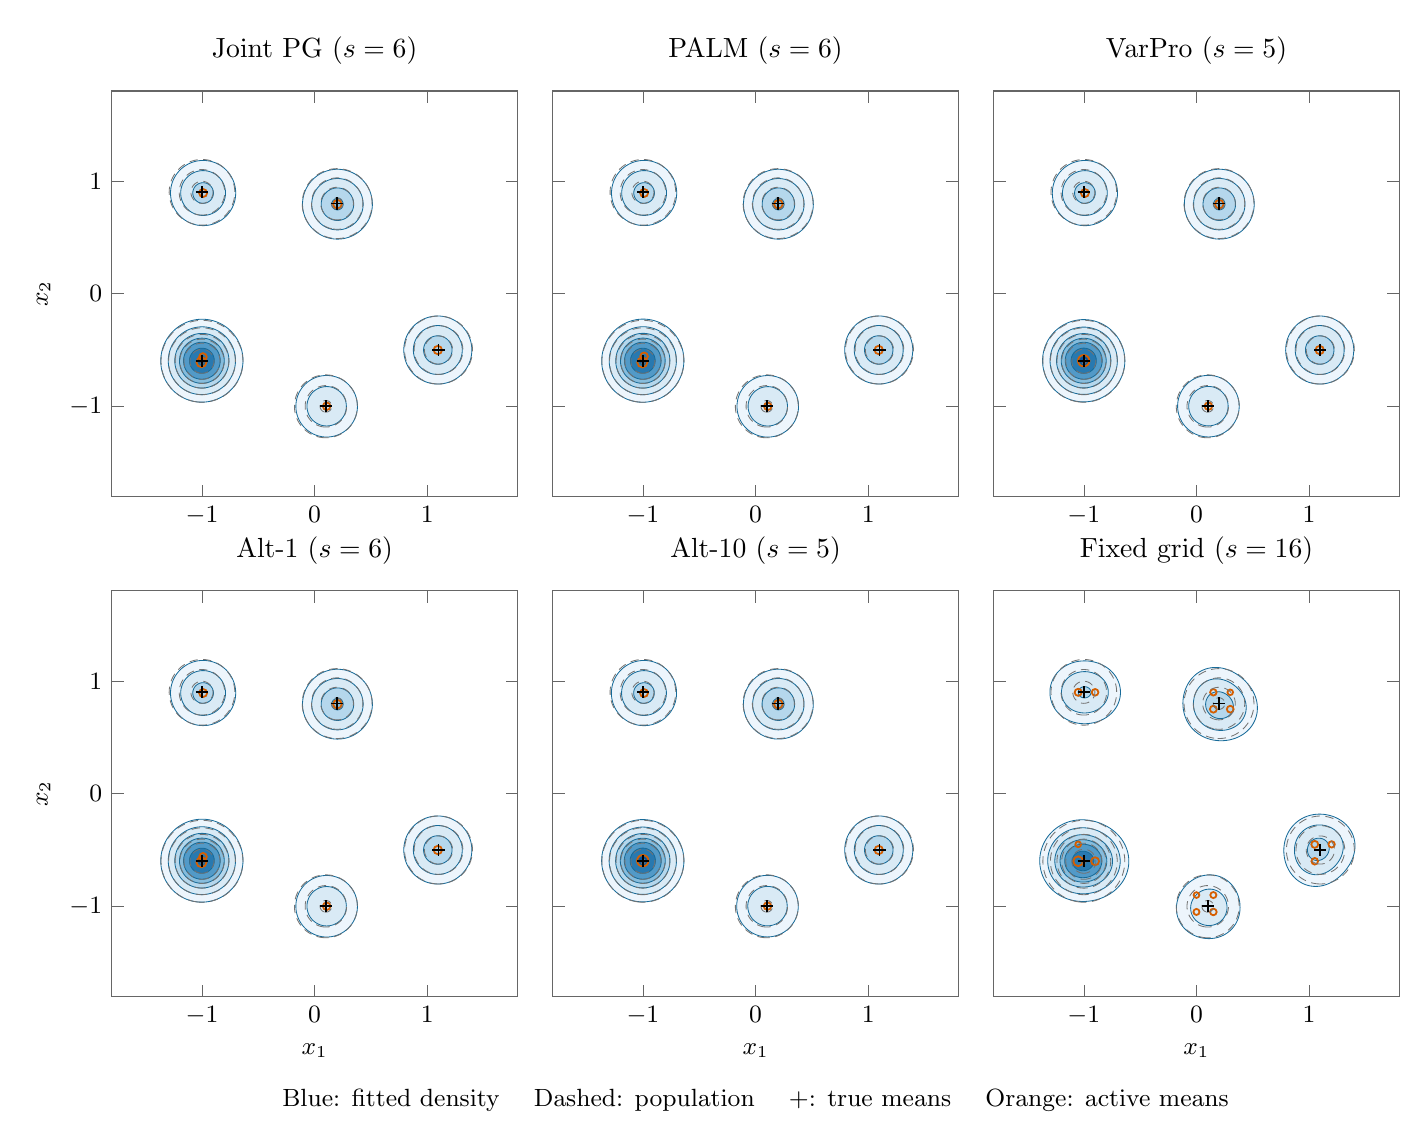
\begin{tikzpicture}
\begin{groupplot}[group style={group size=3 by 2,horizontal sep=0.45cm,vertical sep=1.2cm},
width=5.15cm,height=5.15cm,scale only axis,axis equal image,
xmin=-1.8,xmax=1.8,ymin=-1.8,ymax=1.8,
xtick={-1,0,1},ytick={-1,0,1},tick label style={font=\small},
title style={font=\normalsize},label style={font=\small},
axis line style={black!60},tick style={black!60},
axis background/.style={fill=white},clip=true]
\nextgroupplot[title={Joint PG ($s=6$)},ylabel={$x_2$}]
\path[fill=sketchblue0,draw=sketchline,line width=.3pt,even odd rule] (axis cs:0.06884495,-1.27000000) -- (axis cs:0.08000000,-1.27136049) -- (axis cs:0.09500000,-1.27242963) -- (axis cs:0.11000000,-1.27266685) -- (axis cs:0.12000000,-1.27236738) -- (axis cs:0.13500000,-1.27122170) -- (axis cs:0.15000000,-1.26923980) -- (axis cs:0.16000000,-1.26746077) -- (axis cs:0.17500000,-1.26403375) -- (axis cs:0.18500000,-1.26125695) -- (axis cs:0.19500000,-1.25806546) -- (axis cs:0.20000000,-1.25630229) -- (axis cs:0.21000000,-1.25245682) -- (axis cs:0.22000000,-1.24814325) -- (axis cs:0.22500000,-1.24579827) -- (axis cs:0.23000000,-1.24334449) -- (axis cs:0.24000000,-1.23803320) -- (axis cs:0.25000000,-1.23217080) -- (axis cs:0.26000000,-1.22570609) -- (axis cs:0.27000000,-1.21861047) -- (axis cs:0.28000000,-1.21079529) -- (axis cs:0.29000000,-1.20219766) -- (axis cs:0.30000000,-1.19269534) -- (axis cs:0.31000000,-1.18215471) -- (axis cs:0.31500000,-1.17643684) -- (axis cs:0.32000000,-1.17038028) -- (axis cs:0.32794219,-1.16000000) -- (axis cs:0.33485877,-1.15000000) -- (axis cs:0.34117042,-1.14000000) -- (axis cs:0.34689433,-1.13000000) -- (axis cs:0.35207394,-1.12000000) -- (axis cs:0.35445868,-1.11500000) -- (axis cs:0.35889430,-1.10500000) -- (axis cs:0.36286328,-1.09500000) -- (axis cs:0.36465906,-1.09000000) -- (axis cs:0.36797695,-1.08000000) -- (axis cs:0.37214626,-1.06500000) -- (axis cs:0.37539639,-1.05000000) -- (axis cs:0.37630358,-1.04500000) -- (axis cs:0.37781345,-1.03500000) -- (axis cs:0.37935308,-1.02000000) -- (axis cs:0.38006493,-1.00500000) -- (axis cs:0.38008893,-0.99500000) -- (axis cs:0.37944583,-0.98000000) -- (axis cs:0.37797878,-0.96500000) -- (axis cs:0.37651995,-0.95500000) -- (axis cs:0.37361833,-0.94000000) -- (axis cs:0.37119271,-0.93000000) -- (axis cs:0.36836813,-0.92000000) -- (axis cs:0.36679917,-0.91500000) -- (axis cs:0.36333733,-0.90500000) -- (axis cs:0.36144037,-0.90000000) -- (axis cs:0.35731119,-0.89000000) -- (axis cs:0.35270213,-0.88000000) -- (axis cs:0.34759005,-0.87000000) -- (axis cs:0.34194097,-0.86000000) -- (axis cs:0.33889882,-0.85500000) -- (axis cs:0.33237556,-0.84500000) -- (axis cs:0.32518037,-0.83500000) -- (axis cs:0.31729353,-0.82500000) -- (axis cs:0.30858710,-0.81500000) -- (axis cs:0.29896914,-0.80500000) -- (axis cs:0.28829753,-0.79500000) -- (axis cs:0.28250511,-0.79000000) -- (axis cs:0.27636576,-0.78500000) -- (axis cs:0.26500000,-0.77647015) -- (axis cs:0.25500000,-0.76971005) -- (axis cs:0.24500000,-0.76354554) -- (axis cs:0.23500000,-0.75795979) -- (axis cs:0.22500000,-0.75290839) -- (axis cs:0.22000000,-0.75058428) -- (axis cs:0.21000000,-0.74626482) -- (axis cs:0.20000000,-0.74240841) -- (axis cs:0.19500000,-0.74066227) -- (axis cs:0.18500000,-0.73745307) -- (axis cs:0.17000000,-0.73343834) -- (axis cs:0.16000000,-0.73126155) -- (axis cs:0.14500000,-0.72871717) -- (axis cs:0.13500000,-0.72748748) -- (axis cs:0.12000000,-0.72635415) -- (axis cs:0.10500000,-0.72604562) -- (axis cs:0.09000000,-0.72655260) -- (axis cs:0.07500000,-0.72789039) -- (axis cs:0.06500000,-0.72926281) -- (axis cs:0.05000000,-0.73200463) -- (axis cs:0.04000000,-0.73434026) -- (axis cs:0.03000000,-0.73705214) -- (axis cs:0.01500000,-0.74192103) -- (axis cs:0.01000000,-0.74376470) -- (axis cs:0.00000000,-0.74777530) -- (axis cs:-0.01000000,-0.75226115) -- (axis cs:-0.02000000,-0.75724284) -- (axis cs:-0.03000000,-0.76275153) -- (axis cs:-0.03500000,-0.76572453) -- (axis cs:-0.04500000,-0.77208801) -- (axis cs:-0.05620155,-0.78000000) -- (axis cs:-0.06500000,-0.78680978) -- (axis cs:-0.07500000,-0.79530961) -- (axis cs:-0.08532315,-0.80500000) -- (axis cs:-0.09500000,-0.81507053) -- (axis cs:-0.10364859,-0.82500000) -- (axis cs:-0.11154998,-0.83500000) -- (axis cs:-0.12000000,-0.84689218) -- (axis cs:-0.12829799,-0.86000000) -- (axis cs:-0.13118793,-0.86500000) -- (axis cs:-0.13656617,-0.87500000) -- (axis cs:-0.14142191,-0.88500000) -- (axis cs:-0.14366455,-0.89000000) -- (axis cs:-0.14780228,-0.90000000) -- (axis cs:-0.15147887,-0.91000000) -- (axis cs:-0.15315751,-0.91500000) -- (axis cs:-0.15618797,-0.92500000) -- (axis cs:-0.15881252,-0.93500000) -- (axis cs:-0.16201077,-0.95000000) -- (axis cs:-0.16365171,-0.96000000) -- (axis cs:-0.16540013,-0.97500000) -- (axis cs:-0.16634053,-0.99000000) -- (axis cs:-0.16644353,-1.00500000) -- (axis cs:-0.16604954,-1.01500000) -- (axis cs:-0.16476159,-1.03000000) -- (axis cs:-0.16266761,-1.04500000) -- (axis cs:-0.16076918,-1.05500000) -- (axis cs:-0.15721706,-1.07000000) -- (axis cs:-0.15273871,-1.08500000) -- (axis cs:-0.14921104,-1.09500000) -- (axis cs:-0.14729756,-1.10000000) -- (axis cs:-0.14310346,-1.11000000) -- (axis cs:-0.13842979,-1.12000000) -- (axis cs:-0.13325185,-1.13000000) -- (axis cs:-0.12753401,-1.14000000) -- (axis cs:-0.12444770,-1.14500000) -- (axis cs:-0.11784902,-1.15500000) -- (axis cs:-0.11057030,-1.16500000) -- (axis cs:-0.10258112,-1.17500000) -- (axis cs:-0.09376342,-1.18500000) -- (axis cs:-0.08500000,-1.19403915) -- (axis cs:-0.07500000,-1.20341468) -- (axis cs:-0.06500000,-1.21190668) -- (axis cs:-0.05445787,-1.22000000) -- (axis cs:-0.04500000,-1.22662644) -- (axis cs:-0.03500000,-1.23300041) -- (axis cs:-0.03000000,-1.23595728) -- (axis cs:-0.02000000,-1.24146996) -- (axis cs:-0.01000000,-1.24645133) -- (axis cs:-0.00500000,-1.24875273) -- (axis cs:0.00500000,-1.25300548) -- (axis cs:0.01500000,-1.25679443) -- (axis cs:0.02000000,-1.25852178) -- (axis cs:0.03500000,-1.26307666) -- (axis cs:0.04500000,-1.26558559) -- (axis cs:0.05500000,-1.26772647) -- cycle (axis cs:-1.04886980,-0.96000000) -- (axis cs:-1.04000000,-0.96106439) -- (axis cs:-1.03000000,-0.96197442) -- (axis cs:-1.01500000,-0.96280104) -- (axis cs:-1.00500000,-0.96300407) -- (axis cs:-0.99500000,-0.96293246) -- (axis cs:-0.98000000,-0.96230719) -- (axis cs:-0.96500000,-0.96104253) -- (axis cs:-0.95500000,-0.95983727) -- (axis cs:-0.94500000,-0.95840164) -- (axis cs:-0.93000000,-0.95564654) -- (axis cs:-0.92000000,-0.95347309) -- (axis cs:-0.91000000,-0.95097586) -- (axis cs:-0.89500000,-0.94668175) -- (axis cs:-0.88000000,-0.94166693) -- (axis cs:-0.87000000,-0.93791774) -- (axis cs:-0.86000000,-0.93381598) -- (axis cs:-0.84500000,-0.92702071) -- (axis cs:-0.83500000,-0.92202008) -- (axis cs:-0.82500000,-0.91662487) -- (axis cs:-0.81000000,-0.90776184) -- (axis cs:-0.79500000,-0.89788719) -- (axis cs:-0.78000000,-0.88690332) -- (axis cs:-0.77134716,-0.88000000) -- (axis cs:-0.76539414,-0.87500000) -- (axis cs:-0.75418809,-0.86500000) -- (axis cs:-0.74891454,-0.86000000) -- (axis cs:-0.74000000,-0.85107230) -- (axis cs:-0.72975445,-0.84000000) -- (axis cs:-0.72500000,-0.83454562) -- (axis cs:-0.71709425,-0.82500000) -- (axis cs:-0.71317446,-0.82000000) -- (axis cs:-0.70574767,-0.81000000) -- (axis cs:-0.70220487,-0.80500000) -- (axis cs:-0.69552895,-0.79500000) -- (axis cs:-0.69233406,-0.79000000) -- (axis cs:-0.68631951,-0.78000000) -- (axis cs:-0.67805681,-0.76500000) -- (axis cs:-0.67303897,-0.75500000) -- (axis cs:-0.66839325,-0.74500000) -- (axis cs:-0.66207538,-0.73000000) -- (axis cs:-0.65651920,-0.71500000) -- (axis cs:-0.65167404,-0.70000000) -- (axis cs:-0.64883646,-0.69000000) -- (axis cs:-0.64628751,-0.68000000) -- (axis cs:-0.64403955,-0.67000000) -- (axis cs:-0.64205743,-0.66000000) -- (axis cs:-0.64039986,-0.65000000) -- (axis cs:-0.63897849,-0.64000000) -- (axis cs:-0.63736819,-0.62500000) -- (axis cs:-0.63664906,-0.61500000) -- (axis cs:-0.63620189,-0.60500000) -- (axis cs:-0.63602090,-0.59500000) -- (axis cs:-0.63610380,-0.58500000) -- (axis cs:-0.63672646,-0.57000000) -- (axis cs:-0.63796511,-0.55500000) -- (axis cs:-0.63915075,-0.54500000) -- (axis cs:-0.64060128,-0.53500000) -- (axis cs:-0.64327571,-0.52000000) -- (axis cs:-0.64545158,-0.51000000) -- (axis cs:-0.64787032,-0.50000000) -- (axis cs:-0.65209843,-0.48500000) -- (axis cs:-0.65533024,-0.47500000) -- (axis cs:-0.65883391,-0.46500000) -- (axis cs:-0.66267295,-0.45500000) -- (axis cs:-0.66686459,-0.44500000) -- (axis cs:-0.67382308,-0.43000000) -- (axis cs:-0.68161481,-0.41500000) -- (axis cs:-0.68731119,-0.40500000) -- (axis cs:-0.69034441,-0.40000000) -- (axis cs:-0.69667515,-0.39000000) -- (axis cs:-0.70005142,-0.38500000) -- (axis cs:-0.70708990,-0.37500000) -- (axis cs:-0.71082898,-0.37000000) -- (axis cs:-0.71868795,-0.36000000) -- (axis cs:-0.72283272,-0.35500000) -- (axis cs:-0.73000000,-0.34678289) -- (axis cs:-0.73500000,-0.34132737) -- (axis cs:-0.74606539,-0.33000000) -- (axis cs:-0.75126807,-0.32500000) -- (axis cs:-0.76000000,-0.31702872) -- (axis cs:-0.76822257,-0.31000000) -- (axis cs:-0.77500000,-0.30451099) -- (axis cs:-0.78500000,-0.29686403) -- (axis cs:-0.79000000,-0.29325072) -- (axis cs:-0.80500000,-0.28315528) -- (axis cs:-0.81500000,-0.27700778) -- (axis cs:-0.82000000,-0.27411216) -- (axis cs:-0.83500000,-0.26600842) -- (axis cs:-0.85000000,-0.25878718) -- (axis cs:-0.86500000,-0.25238544) -- (axis cs:-0.87500000,-0.24856719) -- (axis cs:-0.88500000,-0.24510526) -- (axis cs:-0.89500000,-0.24190684) -- (axis cs:-0.90500000,-0.23907159) -- (axis cs:-0.92000000,-0.23538698) -- (axis cs:-0.93500000,-0.23233373) -- (axis cs:-0.94500000,-0.23070285) -- (axis cs:-0.95500000,-0.22933979) -- (axis cs:-0.97000000,-0.22780205) -- (axis cs:-0.98000000,-0.22714192) -- (axis cs:-0.99000000,-0.22676268) -- (axis cs:-1.00000000,-0.22665911) -- (axis cs:-1.01000000,-0.22682969) -- (axis cs:-1.02000000,-0.22727653) -- (axis cs:-1.03000000,-0.22800547) -- (axis cs:-1.04000000,-0.22902618) -- (axis cs:-1.05000000,-0.23032994) -- (axis cs:-1.06500000,-0.23276700) -- (axis cs:-1.07500000,-0.23480767) -- (axis cs:-1.08500000,-0.23707572) -- (axis cs:-1.10000000,-0.24110411) -- (axis cs:-1.11000000,-0.24417449) -- (axis cs:-1.12000000,-0.24754004) -- (axis cs:-1.13500000,-0.25323566) -- (axis cs:-1.14500000,-0.25745463) -- (axis cs:-1.15000000,-0.25972772) -- (axis cs:-1.15500000,-0.26203485) -- (axis cs:-1.16500000,-0.26698552) -- (axis cs:-1.17500000,-0.27232284) -- (axis cs:-1.18000000,-0.27517283) -- (axis cs:-1.18500000,-0.27807052) -- (axis cs:-1.19500000,-0.28426059) -- (axis cs:-1.20000000,-0.28750126) -- (axis cs:-1.21000000,-0.29438867) -- (axis cs:-1.21767457,-0.30000000) -- (axis cs:-1.22500000,-0.30564523) -- (axis cs:-1.23500000,-0.31383718) -- (axis cs:-1.24000000,-0.31815732) -- (axis cs:-1.25281819,-0.33000000) -- (axis cs:-1.26500000,-0.34236196) -- (axis cs:-1.27635078,-0.35500000) -- (axis cs:-1.28055227,-0.36000000) -- (axis cs:-1.28855340,-0.37000000) -- (axis cs:-1.29234688,-0.37500000) -- (axis cs:-1.29951715,-0.38500000) -- (axis cs:-1.30294734,-0.39000000) -- (axis cs:-1.30940296,-0.40000000) -- (axis cs:-1.31249162,-0.40500000) -- (axis cs:-1.31830941,-0.41500000) -- (axis cs:-1.32628204,-0.43000000) -- (axis cs:-1.33341498,-0.44500000) -- (axis cs:-1.33772719,-0.45500000) -- (axis cs:-1.34169056,-0.46500000) -- (axis cs:-1.34703057,-0.48000000) -- (axis cs:-1.35016080,-0.49000000) -- (axis cs:-1.35305113,-0.50000000) -- (axis cs:-1.35677727,-0.51500000) -- (axis cs:-1.35889020,-0.52500000) -- (axis cs:-1.36071839,-0.53500000) -- (axis cs:-1.36296840,-0.55000000) -- (axis cs:-1.36409441,-0.56000000) -- (axis cs:-1.36493932,-0.57000000) -- (axis cs:-1.36554988,-0.58000000) -- (axis cs:-1.36588385,-0.59000000) -- (axis cs:-1.36586656,-0.60500000) -- (axis cs:-1.36550911,-0.61500000) -- (axis cs:-1.36487820,-0.62500000) -- (axis cs:-1.36400859,-0.63500000) -- (axis cs:-1.36285552,-0.64500000) -- (axis cs:-1.36055885,-0.66000000) -- (axis cs:-1.35767404,-0.67500000) -- (axis cs:-1.35534247,-0.68500000) -- (axis cs:-1.35277432,-0.69500000) -- (axis cs:-1.34983954,-0.70500000) -- (axis cs:-1.34665775,-0.71500000) -- (axis cs:-1.34123240,-0.73000000) -- (axis cs:-1.33721134,-0.74000000) -- (axis cs:-1.33503108,-0.74500000) -- (axis cs:-1.33283293,-0.75000000) -- (axis cs:-1.32809112,-0.76000000) -- (axis cs:-1.32297302,-0.77000000) -- (axis cs:-1.32023906,-0.77500000) -- (axis cs:-1.31745844,-0.78000000) -- (axis cs:-1.31151924,-0.79000000) -- (axis cs:-1.30178104,-0.80500000) -- (axis cs:-1.29829515,-0.81000000) -- (axis cs:-1.29093187,-0.82000000) -- (axis cs:-1.28500000,-0.82757215) -- (axis cs:-1.27886564,-0.83500000) -- (axis cs:-1.27453194,-0.84000000) -- (axis cs:-1.26538685,-0.85000000) -- (axis cs:-1.25500000,-0.86051007) -- (axis cs:-1.25000000,-0.86527199) -- (axis cs:-1.24000000,-0.87429008) -- (axis cs:-1.23000000,-0.88267499) -- (axis cs:-1.22500000,-0.88663473) -- (axis cs:-1.21500000,-0.89413630) -- (axis cs:-1.21000000,-0.89770721) -- (axis cs:-1.20000000,-0.90443332) -- (axis cs:-1.19500000,-0.90764711) -- (axis cs:-1.18500000,-0.91369209) -- (axis cs:-1.17000000,-0.92197994) -- (axis cs:-1.16000000,-0.92700151) -- (axis cs:-1.15000000,-0.93164155) -- (axis cs:-1.13500000,-0.93793347) -- (axis cs:-1.12000000,-0.94344571) -- (axis cs:-1.10500000,-0.94822913) -- (axis cs:-1.09500000,-0.95101209) -- (axis cs:-1.08500000,-0.95350825) -- (axis cs:-1.07500000,-0.95568168) -- (axis cs:-1.06500000,-0.95759812) -- cycle (axis cs:1.05816193,-0.80000000) -- (axis cs:1.07000000,-0.80119926) -- (axis cs:1.08500000,-0.80201357) -- (axis cs:1.10000000,-0.80207452) -- (axis cs:1.11500000,-0.80138394) -- (axis cs:1.13000000,-0.79992482) -- (axis cs:1.14500000,-0.79775597) -- (axis cs:1.16000000,-0.79475486) -- (axis cs:1.17000000,-0.79235069) -- (axis cs:1.17500000,-0.79098909) -- (axis cs:1.19000000,-0.78638011) -- (axis cs:1.20000000,-0.78282597) -- (axis cs:1.20500000,-0.78088458) -- (axis cs:1.21500000,-0.77672196) -- (axis cs:1.22500000,-0.77212115) -- (axis cs:1.23000000,-0.76963302) -- (axis cs:1.23500000,-0.76706466) -- (axis cs:1.24500000,-0.76152562) -- (axis cs:1.25500000,-0.75546687) -- (axis cs:1.26500000,-0.74888020) -- (axis cs:1.27500000,-0.74169644) -- (axis cs:1.28000000,-0.73786487) -- (axis cs:1.28960770,-0.73000000) -- (axis cs:1.29500000,-0.72529739) -- (axis cs:1.30500000,-0.71595320) -- (axis cs:1.31500000,-0.70569090) -- (axis cs:1.32447783,-0.69500000) -- (axis cs:1.33258326,-0.68500000) -- (axis cs:1.34000000,-0.67497811) -- (axis cs:1.34681462,-0.66500000) -- (axis cs:1.35306162,-0.65500000) -- (axis cs:1.35597826,-0.65000000) -- (axis cs:1.36145614,-0.64000000) -- (axis cs:1.36645302,-0.63000000) -- (axis cs:1.36877886,-0.62500000) -- (axis cs:1.37311405,-0.61500000) -- (axis cs:1.37509651,-0.61000000) -- (axis cs:1.37702555,-0.60500000) -- (axis cs:1.38051745,-0.59500000) -- (axis cs:1.38214359,-0.59000000) -- (axis cs:1.38504867,-0.58000000) -- (axis cs:1.38639876,-0.57500000) -- (axis cs:1.38877947,-0.56500000) -- (axis cs:1.39169375,-0.55000000) -- (axis cs:1.39382091,-0.53500000) -- (axis cs:1.39517413,-0.52000000) -- (axis cs:1.39580846,-0.50500000) -- (axis cs:1.39568217,-0.49000000) -- (axis cs:1.39480170,-0.47500000) -- (axis cs:1.39320219,-0.46000000) -- (axis cs:1.39169461,-0.45000000) -- (axis cs:1.38878058,-0.43500000) -- (axis cs:1.38640008,-0.42500000) -- (axis cs:1.38505010,-0.42000000) -- (axis cs:1.38214519,-0.41000000) -- (axis cs:1.37702744,-0.39500000) -- (axis cs:1.37311614,-0.38500000) -- (axis cs:1.37099664,-0.38000000) -- (axis cs:1.36645547,-0.37000000) -- (axis cs:1.36401004,-0.36500000) -- (axis cs:1.36145882,-0.36000000) -- (axis cs:1.35598121,-0.35000000) -- (axis cs:1.34998742,-0.34000000) -- (axis cs:1.34348440,-0.33000000) -- (axis cs:1.33637410,-0.32000000) -- (axis cs:1.33258720,-0.31500000) -- (axis cs:1.32500000,-0.30561803) -- (axis cs:1.32015761,-0.30000000) -- (axis cs:1.31092312,-0.29000000) -- (axis cs:1.30078544,-0.28000000) -- (axis cs:1.29000000,-0.27032786) -- (axis cs:1.28000000,-0.26213004) -- (axis cs:1.27000000,-0.25464050) -- (axis cs:1.26000000,-0.24773939) -- (axis cs:1.25000000,-0.24142747) -- (axis cs:1.24500000,-0.23846925) -- (axis cs:1.23500000,-0.23293022) -- (axis cs:1.23000000,-0.23036198) -- (axis cs:1.22500000,-0.22787373) -- (axis cs:1.21500000,-0.22327291) -- (axis cs:1.20000000,-0.21716894) -- (axis cs:1.19000000,-0.21361474) -- (axis cs:1.17500000,-0.20900574) -- (axis cs:1.17000000,-0.20764420) -- (axis cs:1.16000000,-0.20524015) -- (axis cs:1.14500000,-0.20223895) -- (axis cs:1.13000000,-0.20007021) -- (axis cs:1.11500000,-0.19861091) -- (axis cs:1.10000000,-0.19792037) -- (axis cs:1.08500000,-0.19798131) -- (axis cs:1.07000000,-0.19879558) -- (axis cs:1.05500000,-0.20036890) -- (axis cs:1.04000000,-0.20266984) -- (axis cs:1.02500000,-0.20578942) -- (axis cs:1.01500000,-0.20829550) -- (axis cs:1.01000000,-0.20971149) -- (axis cs:1.00000000,-0.21276188) -- (axis cs:0.98500000,-0.21810020) -- (axis cs:0.97500000,-0.22216357) -- (axis cs:0.97000000,-0.22436895) -- (axis cs:0.96500000,-0.22665666) -- (axis cs:0.95500000,-0.23159502) -- (axis cs:0.94500000,-0.23700329) -- (axis cs:0.93500000,-0.24291609) -- (axis cs:0.93000000,-0.24607872) -- (axis cs:0.91694449,-0.25500000) -- (axis cs:0.90500000,-0.26407081) -- (axis cs:0.90000000,-0.26815338) -- (axis cs:0.89209651,-0.27500000) -- (axis cs:0.88146492,-0.28500000) -- (axis cs:0.87178804,-0.29500000) -- (axis cs:0.86294913,-0.30500000) -- (axis cs:0.85881905,-0.31000000) -- (axis cs:0.85107087,-0.32000000) -- (axis cs:0.84396203,-0.33000000) -- (axis cs:0.83743175,-0.34000000) -- (axis cs:0.83145633,-0.35000000) -- (axis cs:0.82865965,-0.35500000) -- (axis cs:0.82342641,-0.36500000) -- (axis cs:0.81644065,-0.38000000) -- (axis cs:0.81231809,-0.39000000) -- (axis cs:0.80690654,-0.40500000) -- (axis cs:0.80236373,-0.42000000) -- (axis cs:0.79866046,-0.43500000) -- (axis cs:0.79575933,-0.45000000) -- (axis cs:0.79361850,-0.46500000) -- (axis cs:0.79224084,-0.48000000) -- (axis cs:0.79162299,-0.49500000) -- (axis cs:0.79174628,-0.51000000) -- (axis cs:0.79261443,-0.52500000) -- (axis cs:0.79425373,-0.54000000) -- (axis cs:0.79663136,-0.55500000) -- (axis cs:0.79982739,-0.57000000) -- (axis cs:0.80236496,-0.58000000) -- (axis cs:0.80379251,-0.58500000) -- (axis cs:0.80690802,-0.59500000) -- (axis cs:0.81231986,-0.61000000) -- (axis cs:0.81866205,-0.62500000) -- (axis cs:0.82342872,-0.63500000) -- (axis cs:0.82599075,-0.64000000) -- (axis cs:0.83145897,-0.65000000) -- (axis cs:0.83743468,-0.66000000) -- (axis cs:0.84063841,-0.66500000) -- (axis cs:0.84396529,-0.67000000) -- (axis cs:0.85000000,-0.67852948) -- (axis cs:0.85882300,-0.69000000) -- (axis cs:0.86295325,-0.69500000) -- (axis cs:0.87000000,-0.70303765) -- (axis cs:0.88000000,-0.71353917) -- (axis cs:0.89000000,-0.72310352) -- (axis cs:0.90000000,-0.73184159) -- (axis cs:0.91000000,-0.73982928) -- (axis cs:0.92000000,-0.74718766) -- (axis cs:0.93000000,-0.75391628) -- (axis cs:0.93500000,-0.75707883) -- (axis cs:0.94500000,-0.76299165) -- (axis cs:0.95500000,-0.76839993) -- (axis cs:0.96000000,-0.77091919) -- (axis cs:0.96500000,-0.77333829) -- (axis cs:0.97500000,-0.77783136) -- (axis cs:0.98500000,-0.78189468) -- (axis cs:1.00000000,-0.78723302) -- (axis cs:1.01500000,-0.79169937) -- (axis cs:1.03000000,-0.79531991) -- (axis cs:1.04500000,-0.79818331) -- cycle (axis cs:0.18590034,0.48500000) -- (axis cs:0.20000000,0.48454163) -- (axis cs:0.21500000,0.48478165) -- (axis cs:0.23000000,0.48573299) -- (axis cs:0.24500000,0.48741407) -- (axis cs:0.26000000,0.48988770) -- (axis cs:0.27500000,0.49306973) -- (axis cs:0.29000000,0.49706853) -- (axis cs:0.30500000,0.50189135) -- (axis cs:0.32000000,0.50757543) -- (axis cs:0.33000000,0.51187297) -- (axis cs:0.33500000,0.51419028) -- (axis cs:0.34000000,0.51659644) -- (axis cs:0.35000000,0.52176479) -- (axis cs:0.36000000,0.52740614) -- (axis cs:0.37000000,0.53355873) -- (axis cs:0.37500000,0.53683064) -- (axis cs:0.38500000,0.54381122) -- (axis cs:0.39320933,0.55000000) -- (axis cs:0.39945493,0.55500000) -- (axis cs:0.41000000,0.56405712) -- (axis cs:0.41500000,0.56865166) -- (axis cs:0.42155854,0.57500000) -- (axis cs:0.43115148,0.58500000) -- (axis cs:0.44000000,0.59508885) -- (axis cs:0.44500000,0.60118612) -- (axis cs:0.45179377,0.61000000) -- (axis cs:0.45889774,0.62000000) -- (axis cs:0.46224215,0.62500000) -- (axis cs:0.46850549,0.63500000) -- (axis cs:0.47144424,0.64000000) -- (axis cs:0.47695843,0.65000000) -- (axis cs:0.48200304,0.66000000) -- (axis cs:0.48874263,0.67500000) -- (axis cs:0.49272877,0.68500000) -- (axis cs:0.49454984,0.69000000) -- (axis cs:0.49796222,0.70000000) -- (axis cs:0.49949946,0.70500000) -- (axis cs:0.50363387,0.72000000) -- (axis cs:0.50696558,0.73500000) -- (axis cs:0.50950467,0.75000000) -- (axis cs:0.51132707,0.76500000) -- (axis cs:0.51240699,0.78000000) -- (axis cs:0.51275077,0.79500000) -- (axis cs:0.51236879,0.81000000) -- (axis cs:0.51124953,0.82500000) -- (axis cs:0.50939146,0.84000000) -- (axis cs:0.50680926,0.85500000) -- (axis cs:0.50343956,0.87000000) -- (axis cs:0.49926496,0.88500000) -- (axis cs:0.49603528,0.89500000) -- (axis cs:0.49243014,0.90500000) -- (axis cs:0.49045558,0.91000000) -- (axis cs:0.48841534,0.91500000) -- (axis cs:0.48398587,0.92500000) -- (axis cs:0.48161982,0.93000000) -- (axis cs:0.47653908,0.94000000) -- (axis cs:0.47098485,0.95000000) -- (axis cs:0.46803397,0.95500000) -- (axis cs:0.46172379,0.96500000) -- (axis cs:0.45484337,0.97500000) -- (axis cs:0.45120410,0.98000000) -- (axis cs:0.44500000,0.98802901) -- (axis cs:0.43926970,0.99500000) -- (axis cs:0.43493378,1.00000000) -- (axis cs:0.42500000,1.01072117) -- (axis cs:0.41500000,1.02055401) -- (axis cs:0.40447505,1.03000000) -- (axis cs:0.39849731,1.03500000) -- (axis cs:0.39000000,1.04169162) -- (axis cs:0.38000000,1.04896079) -- (axis cs:0.37500000,1.05238361) -- (axis cs:0.36500000,1.05879096) -- (axis cs:0.36000000,1.06180452) -- (axis cs:0.35000000,1.06745006) -- (axis cs:0.34000000,1.07261965) -- (axis cs:0.33000000,1.07734125) -- (axis cs:0.31500000,1.08362554) -- (axis cs:0.30000000,1.08901302) -- (axis cs:0.28500000,1.09356223) -- (axis cs:0.27000000,1.09730061) -- (axis cs:0.26000000,1.09933694) -- (axis cs:0.25000000,1.10105664) -- (axis cs:0.23500000,1.10301093) -- (axis cs:0.22000000,1.10420352) -- (axis cs:0.20500000,1.10467071) -- (axis cs:0.19000000,1.10442659) -- (axis cs:0.17500000,1.10346381) -- (axis cs:0.16000000,1.10175317) -- (axis cs:0.14500000,1.09928016) -- (axis cs:0.13000000,1.09606030) -- (axis cs:0.11500000,1.09205377) -- (axis cs:0.10000000,1.08721521) -- (axis cs:0.08500000,1.08150707) -- (axis cs:0.07500000,1.07720269) -- (axis cs:0.06500000,1.07246805) -- (axis cs:0.06000000,1.06990884) -- (axis cs:0.05500000,1.06728411) -- (axis cs:0.04500000,1.06162261) -- (axis cs:0.04000000,1.05860413) -- (axis cs:0.03000000,1.05217806) -- (axis cs:0.02000000,1.04516488) -- (axis cs:0.01500000,1.04145740) -- (axis cs:0.00680820,1.03500000) -- (axis cs:-0.00500000,1.02486998) -- (axis cs:-0.01545064,1.01500000) -- (axis cs:-0.02510885,1.00500000) -- (axis cs:-0.03500000,0.99376658) -- (axis cs:-0.04209303,0.98500000) -- (axis cs:-0.04589449,0.98000000) -- (axis cs:-0.05305899,0.97000000) -- (axis cs:-0.05641514,0.96500000) -- (axis cs:-0.06272845,0.95500000) -- (axis cs:-0.06851820,0.94500000) -- (axis cs:-0.07122968,0.94000000) -- (axis cs:-0.07631054,0.93000000) -- (axis cs:-0.08311101,0.91500000) -- (axis cs:-0.08896973,0.90000000) -- (axis cs:-0.09396329,0.88500000) -- (axis cs:-0.09813550,0.87000000) -- (axis cs:-0.10150012,0.85500000) -- (axis cs:-0.10409046,0.84000000) -- (axis cs:-0.10593850,0.82500000) -- (axis cs:-0.10706139,0.81000000) -- (axis cs:-0.10744461,0.79500000) -- (axis cs:-0.10709971,0.78000000) -- (axis cs:-0.10601629,0.76500000) -- (axis cs:-0.10420402,0.75000000) -- (axis cs:-0.10165693,0.73500000) -- (axis cs:-0.09833040,0.72000000) -- (axis cs:-0.09419849,0.70500000) -- (axis cs:-0.09265666,0.70000000) -- (axis cs:-0.08924886,0.69000000) -- (axis cs:-0.08742251,0.68500000) -- (axis cs:-0.08343922,0.67500000) -- (axis cs:-0.07669480,0.66000000) -- (axis cs:-0.07165013,0.65000000) -- (axis cs:-0.06613470,0.64000000) -- (axis cs:-0.06320112,0.63500000) -- (axis cs:-0.05693472,0.62500000) -- (axis cs:-0.05359412,0.62000000) -- (axis cs:-0.04648544,0.61000000) -- (axis cs:-0.04000000,0.60156932) -- (axis cs:-0.03500000,0.59545096) -- (axis cs:-0.02584233,0.58500000) -- (axis cs:-0.01625035,0.57500000) -- (axis cs:-0.00500000,0.56433594) -- (axis cs:0.00584953,0.55500000) -- (axis cs:0.01209655,0.55000000) -- (axis cs:0.02000000,0.54403667) -- (axis cs:0.03000000,0.53703497) -- (axis cs:0.03500000,0.53375727) -- (axis cs:0.04500000,0.52758688) -- (axis cs:0.05500000,0.52192965) -- (axis cs:0.06500000,0.51674700) -- (axis cs:0.07000000,0.51433745) -- (axis cs:0.07500000,0.51201055) -- (axis cs:0.08500000,0.50770111) -- (axis cs:0.09500000,0.50380803) -- (axis cs:0.11000000,0.49868448) -- (axis cs:0.12500000,0.49440948) -- (axis cs:0.14000000,0.49091795) -- (axis cs:0.15500000,0.48819515) -- (axis cs:0.17000000,0.48624085) -- cycle (axis cs:-1.00894571,0.60500000) -- (axis cs:-0.99500000,0.60440381) -- (axis cs:-0.98000000,0.60453695) -- (axis cs:-0.96500000,0.60544746) -- (axis cs:-0.95500000,0.60647614) -- (axis cs:-0.94000000,0.60870776) -- (axis cs:-0.92500000,0.61174789) -- (axis cs:-0.91000000,0.61564616) -- (axis cs:-0.90000000,0.61871273) -- (axis cs:-0.89000000,0.62218496) -- (axis cs:-0.87500000,0.62819437) -- (axis cs:-0.86500000,0.63275331) -- (axis cs:-0.86000000,0.63522826) -- (axis cs:-0.85500000,0.63778569) -- (axis cs:-0.84500000,0.64332022) -- (axis cs:-0.84000000,0.64628711) -- (axis cs:-0.83000000,0.65263044) -- (axis cs:-0.82000000,0.65959079) -- (axis cs:-0.81000000,0.66717841) -- (axis cs:-0.80000000,0.67551092) -- (axis cs:-0.79000000,0.68464182) -- (axis cs:-0.78000000,0.69469079) -- (axis cs:-0.77068511,0.70500000) -- (axis cs:-0.76245287,0.71500000) -- (axis cs:-0.75861624,0.72000000) -- (axis cs:-0.75143504,0.73000000) -- (axis cs:-0.74488717,0.74000000) -- (axis cs:-0.73888015,0.75000000) -- (axis cs:-0.73341129,0.76000000) -- (axis cs:-0.73087363,0.76500000) -- (axis cs:-0.72844261,0.77000000) -- (axis cs:-0.72394688,0.78000000) -- (axis cs:-0.72185789,0.78500000) -- (axis cs:-0.71801636,0.79500000) -- (axis cs:-0.71303089,0.81000000) -- (axis cs:-0.71022459,0.82000000) -- (axis cs:-0.70775646,0.83000000) -- (axis cs:-0.70667669,0.83500000) -- (axis cs:-0.70398498,0.85000000) -- (axis cs:-0.70262437,0.86000000) -- (axis cs:-0.70126625,0.87500000) -- (axis cs:-0.70069259,0.89000000) -- (axis cs:-0.70088607,0.90500000) -- (axis cs:-0.70185251,0.92000000) -- (axis cs:-0.70362121,0.93500000) -- (axis cs:-0.70619062,0.95000000) -- (axis cs:-0.70835441,0.96000000) -- (axis cs:-0.71230978,0.97500000) -- (axis cs:-0.71714947,0.99000000) -- (axis cs:-0.72291768,1.00500000) -- (axis cs:-0.72730817,1.01500000) -- (axis cs:-0.73216180,1.02500000) -- (axis cs:-0.73750364,1.03500000) -- (axis cs:-0.74038371,1.04000000) -- (axis cs:-0.74650831,1.05000000) -- (axis cs:-0.75322453,1.06000000) -- (axis cs:-0.75681663,1.06500000) -- (axis cs:-0.76451477,1.07500000) -- (axis cs:-0.77292399,1.08500000) -- (axis cs:-0.78216465,1.09500000) -- (axis cs:-0.79234102,1.10500000) -- (axis cs:-0.80360817,1.11500000) -- (axis cs:-0.81500000,1.12411996) -- (axis cs:-0.82500000,1.13139011) -- (axis cs:-0.83500000,1.13803454) -- (axis cs:-0.84000000,1.14113144) -- (axis cs:-0.85000000,1.14693161) -- (axis cs:-0.86000000,1.15221097) -- (axis cs:-0.87000000,1.15700354) -- (axis cs:-0.88500000,1.16333747) -- (axis cs:-0.89500000,1.16702474) -- (axis cs:-0.90000000,1.16870728) -- (axis cs:-0.91500000,1.17317750) -- (axis cs:-0.93000000,1.17677890) -- (axis cs:-0.94000000,1.17871219) -- (axis cs:-0.95500000,1.18093717) -- (axis cs:-0.97000000,1.18238243) -- (axis cs:-0.98500000,1.18303120) -- (axis cs:-1.00000000,1.18290309) -- (axis cs:-1.01500000,1.18199425) -- (axis cs:-1.02500000,1.18094202) -- (axis cs:-1.04000000,1.17871899) -- (axis cs:-1.05000000,1.17678727) -- (axis cs:-1.06500000,1.17318797) -- (axis cs:-1.08000000,1.16871999) -- (axis cs:-1.08500000,1.16703842) -- (axis cs:-1.09500000,1.16335264) -- (axis cs:-1.11000000,1.15702149) -- (axis cs:-1.12000000,1.15223074) -- (axis cs:-1.13000000,1.14695338) -- (axis cs:-1.13500000,1.14411544) -- (axis cs:-1.14500000,1.13805933) -- (axis cs:-1.15500000,1.13141753) -- (axis cs:-1.16000000,1.12787052) -- (axis cs:-1.17000000,1.12025879) -- (axis cs:-1.18000000,1.11195258) -- (axis cs:-1.19000000,1.10282561) -- (axis cs:-1.20000000,1.09277942) -- (axis cs:-1.21000000,1.08166623) -- (axis cs:-1.21945539,1.07000000) -- (axis cs:-1.22681486,1.06000000) -- (axis cs:-1.23353064,1.05000000) -- (axis cs:-1.23667025,1.04500000) -- (axis cs:-1.24253557,1.03500000) -- (axis cs:-1.24787731,1.02500000) -- (axis cs:-1.25273098,1.01500000) -- (axis cs:-1.25712166,1.00500000) -- (axis cs:-1.25914052,1.00000000) -- (axis cs:-1.26288962,0.99000000) -- (axis cs:-1.26458534,0.98500000) -- (axis cs:-1.26772936,0.97500000) -- (axis cs:-1.26913321,0.97000000) -- (axis cs:-1.27281808,0.95500000) -- (axis cs:-1.27564223,0.94000000) -- (axis cs:-1.27709967,0.93000000) -- (axis cs:-1.27859566,0.91500000) -- (axis cs:-1.27930211,0.90000000) -- (axis cs:-1.27924038,0.88500000) -- (axis cs:-1.27840862,0.87000000) -- (axis cs:-1.27741488,0.86000000) -- (axis cs:-1.27523172,0.84500000) -- (axis cs:-1.27228283,0.83000000) -- (axis cs:-1.26846797,0.81500000) -- (axis cs:-1.26543008,0.80500000) -- (axis cs:-1.26202301,0.79500000) -- (axis cs:-1.26013335,0.79000000) -- (axis cs:-1.25818111,0.78500000) -- (axis cs:-1.25389964,0.77500000) -- (axis cs:-1.25159688,0.77000000) -- (axis cs:-1.24662818,0.76000000) -- (axis cs:-1.24115945,0.75000000) -- (axis cs:-1.23823524,0.74500000) -- (axis cs:-1.23196266,0.73500000) -- (axis cs:-1.22507973,0.72500000) -- (axis cs:-1.21758632,0.71500000) -- (axis cs:-1.20935374,0.70500000) -- (axis cs:-1.20033274,0.69500000) -- (axis cs:-1.19041274,0.68500000) -- (axis cs:-1.18000000,0.67547712) -- (axis cs:-1.17000000,0.66714731) -- (axis cs:-1.16500000,0.66326403) -- (axis cs:-1.15500000,0.65600582) -- (axis cs:-1.14500000,0.64937131) -- (axis cs:-1.13500000,0.64329737) -- (axis cs:-1.12500000,0.63776496) -- (axis cs:-1.12000000,0.63520888) -- (axis cs:-1.11500000,0.63273449) -- (axis cs:-1.10500000,0.62817729) -- (axis cs:-1.09500000,0.62407454) -- (axis cs:-1.09000000,0.62217056) -- (axis cs:-1.08000000,0.61869976) -- (axis cs:-1.07500000,0.61710788) -- (axis cs:-1.06500000,0.61424334) -- (axis cs:-1.06000000,0.61293667) -- (axis cs:-1.05000000,0.61064580) -- (axis cs:-1.03500000,0.60786281) -- (axis cs:-1.02000000,0.60591323) -- cycle;
\path[fill=sketchblue1,draw=sketchline,line width=.3pt,even odd rule] (axis cs:0.06895869,-1.17000000) -- (axis cs:0.07500000,-1.17124465) -- (axis cs:0.08500000,-1.17279959) -- (axis cs:0.09000000,-1.17335513) -- (axis cs:0.10000000,-1.17403167) -- (axis cs:0.11000000,-1.17413557) -- (axis cs:0.12000000,-1.17366822) -- (axis cs:0.13000000,-1.17262336) -- (axis cs:0.13500000,-1.17188029) -- (axis cs:0.14500000,-1.16994086) -- (axis cs:0.15500000,-1.16739504) -- (axis cs:0.16261900,-1.16500000) -- (axis cs:0.17000000,-1.16234760) -- (axis cs:0.18000000,-1.15810802) -- (axis cs:0.18500000,-1.15570509) -- (axis cs:0.19500000,-1.15029032) -- (axis cs:0.20000000,-1.14725516) -- (axis cs:0.20500000,-1.14398373) -- (axis cs:0.21000000,-1.14046060) -- (axis cs:0.21500000,-1.13666240) -- (axis cs:0.22295141,-1.13000000) -- (axis cs:0.22834546,-1.12500000) -- (axis cs:0.23500000,-1.11820250) -- (axis cs:0.24000000,-1.11256890) -- (axis cs:0.24500000,-1.10641017) -- (axis cs:0.24974439,-1.10000000) -- (axis cs:0.25500000,-1.09206882) -- (axis cs:0.25920717,-1.08500000) -- (axis cs:0.26191241,-1.08000000) -- (axis cs:0.26671644,-1.07000000) -- (axis cs:0.27000000,-1.06199755) -- (axis cs:0.27253575,-1.05500000) -- (axis cs:0.27556206,-1.04500000) -- (axis cs:0.27795685,-1.03500000) -- (axis cs:0.27892093,-1.03000000) -- (axis cs:0.28040268,-1.02000000) -- (axis cs:0.28092648,-1.01500000) -- (axis cs:0.28153831,-1.00500000) -- (axis cs:0.28157513,-0.99500000) -- (axis cs:0.28103742,-0.98500000) -- (axis cs:0.28055117,-0.98000000) -- (axis cs:0.27914401,-0.97000000) -- (axis cs:0.27714060,-0.96000000) -- (axis cs:0.27451216,-0.95000000) -- (axis cs:0.27124012,-0.94000000) -- (axis cs:0.26934645,-0.93500000) -- (axis cs:0.26727785,-0.93000000) -- (axis cs:0.26257343,-0.92000000) -- (axis cs:0.25705821,-0.91000000) -- (axis cs:0.25396851,-0.90500000) -- (axis cs:0.25000000,-0.89908942) -- (axis cs:0.24318749,-0.89000000) -- (axis cs:0.23902292,-0.88500000) -- (axis cs:0.23500000,-0.88050815) -- (axis cs:0.23000000,-0.87533201) -- (axis cs:0.22438570,-0.87000000) -- (axis cs:0.21863204,-0.86500000) -- (axis cs:0.21233047,-0.86000000) -- (axis cs:0.20538981,-0.85500000) -- (axis cs:0.19761896,-0.85000000) -- (axis cs:0.19000000,-0.84561346) -- (axis cs:0.18500000,-0.84301022) -- (axis cs:0.17500000,-0.83839672) -- (axis cs:0.17000000,-0.83636934) -- (axis cs:0.16000000,-0.83283628) -- (axis cs:0.15500000,-0.83132224) -- (axis cs:0.14500000,-0.82877131) -- (axis cs:0.14000000,-0.82772720) -- (axis cs:0.13000000,-0.82609473) -- (axis cs:0.12500000,-0.82550085) -- (axis cs:0.11500000,-0.82474526) -- (axis cs:0.11000000,-0.82458195) -- (axis cs:0.10000000,-0.82468665) -- (axis cs:0.09000000,-0.82536471) -- (axis cs:0.08000000,-0.82661994) -- (axis cs:0.07000000,-0.82847236) -- (axis cs:0.06000000,-0.83093947) -- (axis cs:0.05000000,-0.83404520) -- (axis cs:0.04500000,-0.83585006) -- (axis cs:0.04000000,-0.83782775) -- (axis cs:0.03000000,-0.84233828) -- (axis cs:0.02000000,-0.84764004) -- (axis cs:0.01500000,-0.85061362) -- (axis cs:0.00826311,-0.85500000) -- (axis cs:0.00130824,-0.86000000) -- (axis cs:-0.00500000,-0.86499973) -- (axis cs:-0.01074352,-0.87000000) -- (axis cs:-0.01500000,-0.87400022) -- (axis cs:-0.02000000,-0.87906166) -- (axis cs:-0.02500000,-0.88456029) -- (axis cs:-0.03000000,-0.89056982) -- (axis cs:-0.03500000,-0.89718372) -- (axis cs:-0.04000000,-0.90449829) -- (axis cs:-0.04341619,-0.91000000) -- (axis cs:-0.04628051,-0.91500000) -- (axis cs:-0.05138012,-0.92500000) -- (axis cs:-0.05500000,-0.93328573) -- (axis cs:-0.05759912,-0.94000000) -- (axis cs:-0.06087168,-0.95000000) -- (axis cs:-0.06349788,-0.96000000) -- (axis cs:-0.06457383,-0.96500000) -- (axis cs:-0.06628134,-0.97500000) -- (axis cs:-0.06739764,-0.98500000) -- (axis cs:-0.06793384,-0.99500000) -- (axis cs:-0.06789713,-1.00500000) -- (axis cs:-0.06728701,-1.01500000) -- (axis cs:-0.06609531,-1.02500000) -- (axis cs:-0.06527668,-1.03000000) -- (axis cs:-0.06319647,-1.04000000) -- (axis cs:-0.06048730,-1.05000000) -- (axis cs:-0.05712979,-1.06000000) -- (axis cs:-0.05518950,-1.06500000) -- (axis cs:-0.05076955,-1.07500000) -- (axis cs:-0.04827034,-1.08000000) -- (axis cs:-0.04500000,-1.08598304) -- (axis cs:-0.04000000,-1.09421405) -- (axis cs:-0.03500000,-1.10153479) -- (axis cs:-0.03000000,-1.10813905) -- (axis cs:-0.02500000,-1.11415269) -- (axis cs:-0.01967462,-1.12000000) -- (axis cs:-0.01470963,-1.12500000) -- (axis cs:-0.00931487,-1.13000000) -- (axis cs:-0.00342794,-1.13500000) -- (axis cs:0.00500000,-1.14144284) -- (axis cs:0.01015638,-1.14500000) -- (axis cs:0.02000000,-1.15107603) -- (axis cs:0.02727733,-1.15500000) -- (axis cs:0.03500000,-1.15872674) -- (axis cs:0.04000000,-1.16088719) -- (axis cs:0.05000000,-1.16466912) -- (axis cs:0.06000000,-1.16777853) -- cycle (axis cs:-1.02501866,-0.89500000) -- (axis cs:-1.01000000,-0.89578593) -- (axis cs:-0.99500000,-0.89579284) -- (axis cs:-0.98000000,-0.89502303) -- (axis cs:-0.96500000,-0.89352738) -- (axis cs:-0.95000000,-0.89122630) -- (axis cs:-0.93500000,-0.88813840) -- (axis cs:-0.92000000,-0.88421237) -- (axis cs:-0.91000000,-0.88113567) -- (axis cs:-0.90000000,-0.87767071) -- (axis cs:-0.88500000,-0.87169151) -- (axis cs:-0.87500000,-0.86717254) -- (axis cs:-0.87000000,-0.86472340) -- (axis cs:-0.86500000,-0.86219683) -- (axis cs:-0.85500000,-0.85673905) -- (axis cs:-0.85000000,-0.85381745) -- (axis cs:-0.84000000,-0.84758888) -- (axis cs:-0.83000000,-0.84077621) -- (axis cs:-0.82000000,-0.83336504) -- (axis cs:-0.80969535,-0.82500000) -- (axis cs:-0.79846807,-0.81500000) -- (axis cs:-0.78828952,-0.80500000) -- (axis cs:-0.77901667,-0.79500000) -- (axis cs:-0.77000000,-0.78433196) -- (axis cs:-0.76274928,-0.77500000) -- (axis cs:-0.75911376,-0.77000000) -- (axis cs:-0.75227040,-0.76000000) -- (axis cs:-0.74907606,-0.75500000) -- (axis cs:-0.74306418,-0.74500000) -- (axis cs:-0.73756520,-0.73500000) -- (axis cs:-0.73254285,-0.72500000) -- (axis cs:-0.72797089,-0.71500000) -- (axis cs:-0.72585658,-0.71000000) -- (axis cs:-0.72190748,-0.70000000) -- (axis cs:-0.72011299,-0.69500000) -- (axis cs:-0.71837073,-0.69000000) -- (axis cs:-0.71523776,-0.68000000) -- (axis cs:-0.71243435,-0.67000000) -- (axis cs:-0.71118900,-0.66500000) -- (axis cs:-0.70795456,-0.65000000) -- (axis cs:-0.70552495,-0.63500000) -- (axis cs:-0.70382831,-0.62000000) -- (axis cs:-0.70288245,-0.60500000) -- (axis cs:-0.70268601,-0.59000000) -- (axis cs:-0.70323365,-0.57500000) -- (axis cs:-0.70454204,-0.56000000) -- (axis cs:-0.70657227,-0.54500000) -- (axis cs:-0.70940435,-0.53000000) -- (axis cs:-0.71300286,-0.51500000) -- (axis cs:-0.71744300,-0.50000000) -- (axis cs:-0.72275173,-0.48500000) -- (axis cs:-0.72679917,-0.47500000) -- (axis cs:-0.72898794,-0.47000000) -- (axis cs:-0.73367803,-0.46000000) -- (axis cs:-0.73619726,-0.45500000) -- (axis cs:-0.74158933,-0.44500000) -- (axis cs:-0.74748710,-0.43500000) -- (axis cs:-0.75393710,-0.42500000) -- (axis cs:-0.75736831,-0.42000000) -- (axis cs:-0.76472534,-0.41000000) -- (axis cs:-0.77272360,-0.40000000) -- (axis cs:-0.78148570,-0.39000000) -- (axis cs:-0.79108779,-0.38000000) -- (axis cs:-0.80164864,-0.37000000) -- (axis cs:-0.80733998,-0.36500000) -- (axis cs:-0.81500000,-0.35865506) -- (axis cs:-0.82639177,-0.35000000) -- (axis cs:-0.83500000,-0.34399304) -- (axis cs:-0.84000000,-0.34071608) -- (axis cs:-0.84500000,-0.33756619) -- (axis cs:-0.85500000,-0.33169707) -- (axis cs:-0.86500000,-0.32633969) -- (axis cs:-0.87500000,-0.32145941) -- (axis cs:-0.88000000,-0.31919951) -- (axis cs:-0.88500000,-0.31703171) -- (axis cs:-0.89500000,-0.31304137) -- (axis cs:-0.91000000,-0.30782761) -- (axis cs:-0.92000000,-0.30487099) -- (axis cs:-0.92500000,-0.30350220) -- (axis cs:-0.93500000,-0.30109107) -- (axis cs:-0.95000000,-0.29814286) -- (axis cs:-0.96000000,-0.29662800) -- (axis cs:-0.97500000,-0.29503165) -- (axis cs:-0.99000000,-0.29416458) -- (axis cs:-1.00500000,-0.29407615) -- (axis cs:-1.02000000,-0.29476452) -- (axis cs:-1.03500000,-0.29619030) -- (axis cs:-1.05000000,-0.29840608) -- (axis cs:-1.06500000,-0.30142177) -- (axis cs:-1.07500000,-0.30388759) -- (axis cs:-1.09000000,-0.30827643) -- (axis cs:-1.10000000,-0.31169089) -- (axis cs:-1.11500000,-0.31757099) -- (axis cs:-1.12500000,-0.32202643) -- (axis cs:-1.13000000,-0.32443539) -- (axis cs:-1.13500000,-0.32693144) -- (axis cs:-1.14500000,-0.33230979) -- (axis cs:-1.15500000,-0.33819511) -- (axis cs:-1.16000000,-0.34133977) -- (axis cs:-1.17000000,-0.34804360) -- (axis cs:-1.18000000,-0.35537014) -- (axis cs:-1.19197572,-0.36500000) -- (axis cs:-1.20320282,-0.37500000) -- (axis cs:-1.21338936,-0.38500000) -- (axis cs:-1.22268004,-0.39500000) -- (axis cs:-1.23117268,-0.40500000) -- (axis cs:-1.24000000,-0.41641319) -- (axis cs:-1.24611110,-0.42500000) -- (axis cs:-1.24945587,-0.43000000) -- (axis cs:-1.25268015,-0.43500000) -- (axis cs:-1.25869469,-0.44500000) -- (axis cs:-1.26420247,-0.45500000) -- (axis cs:-1.26678885,-0.46000000) -- (axis cs:-1.27159832,-0.47000000) -- (axis cs:-1.27596439,-0.48000000) -- (axis cs:-1.27800209,-0.48500000) -- (axis cs:-1.28175341,-0.49500000) -- (axis cs:-1.28664917,-0.51000000) -- (axis cs:-1.29069275,-0.52500000) -- (axis cs:-1.29394692,-0.54000000) -- (axis cs:-1.29641857,-0.55500000) -- (axis cs:-1.29812728,-0.57000000) -- (axis cs:-1.29907152,-0.58500000) -- (axis cs:-1.29927864,-0.60000000) -- (axis cs:-1.29875400,-0.61500000) -- (axis cs:-1.29748128,-0.63000000) -- (axis cs:-1.29542165,-0.64500000) -- (axis cs:-1.29262874,-0.66000000) -- (axis cs:-1.28900610,-0.67500000) -- (axis cs:-1.28614122,-0.68500000) -- (axis cs:-1.28290201,-0.69500000) -- (axis cs:-1.27728901,-0.71000000) -- (axis cs:-1.27302612,-0.72000000) -- (axis cs:-1.27072004,-0.72500000) -- (axis cs:-1.26832365,-0.73000000) -- (axis cs:-1.26316091,-0.74000000) -- (axis cs:-1.25750763,-0.75000000) -- (axis cs:-1.25132290,-0.76000000) -- (axis cs:-1.24802774,-0.76500000) -- (axis cs:-1.24097577,-0.77500000) -- (axis cs:-1.23722306,-0.78000000) -- (axis cs:-1.22918156,-0.79000000) -- (axis cs:-1.22000000,-0.80042886) -- (axis cs:-1.21000000,-0.81076477) -- (axis cs:-1.20000000,-0.82015852) -- (axis cs:-1.18845698,-0.83000000) -- (axis cs:-1.18210097,-0.83500000) -- (axis cs:-1.17536263,-0.84000000) -- (axis cs:-1.16500000,-0.84716168) -- (axis cs:-1.15500000,-0.85346021) -- (axis cs:-1.15000000,-0.85640574) -- (axis cs:-1.14000000,-0.86191669) -- (axis cs:-1.13000000,-0.86693660) -- (axis cs:-1.12000000,-0.87149250) -- (axis cs:-1.11500000,-0.87360544) -- (axis cs:-1.10500000,-0.87751964) -- (axis cs:-1.10000000,-0.87930486) -- (axis cs:-1.09000000,-0.88261854) -- (axis cs:-1.08500000,-0.88410999) -- (axis cs:-1.07000000,-0.88806203) -- (axis cs:-1.05500000,-0.89117086) -- (axis cs:-1.04000000,-0.89349119) -- cycle (axis cs:1.06366509,-0.71500000) -- (axis cs:1.07500000,-0.71630487) -- (axis cs:1.08500000,-0.71694119) -- (axis cs:1.09500000,-0.71711309) -- (axis cs:1.10500000,-0.71682287) -- (axis cs:1.11500000,-0.71606665) -- (axis cs:1.12000000,-0.71551087) -- (axis cs:1.13000000,-0.71405799) -- (axis cs:1.14000000,-0.71212604) -- (axis cs:1.15000000,-0.70968348) -- (axis cs:1.16000000,-0.70674949) -- (axis cs:1.17000000,-0.70327160) -- (axis cs:1.18000000,-0.69922737) -- (axis cs:1.19000000,-0.69458879) -- (axis cs:1.20000000,-0.68931376) -- (axis cs:1.21000000,-0.68334432) -- (axis cs:1.22000000,-0.67660420) -- (axis cs:1.22500000,-0.67291936) -- (axis cs:1.23481752,-0.66500000) -- (axis cs:1.24046337,-0.66000000) -- (axis cs:1.24500000,-0.65571882) -- (axis cs:1.25000000,-0.65069962) -- (axis cs:1.25530291,-0.64500000) -- (axis cs:1.26000000,-0.63958686) -- (axis cs:1.26760509,-0.63000000) -- (axis cs:1.27464725,-0.62000000) -- (axis cs:1.28089938,-0.61000000) -- (axis cs:1.28643078,-0.60000000) -- (axis cs:1.29129966,-0.59000000) -- (axis cs:1.29555218,-0.58000000) -- (axis cs:1.29923657,-0.57000000) -- (axis cs:1.30238279,-0.56000000) -- (axis cs:1.30498863,-0.55000000) -- (axis cs:1.30712268,-0.54000000) -- (axis cs:1.30875346,-0.53000000) -- (axis cs:1.30938723,-0.52500000) -- (axis cs:1.31030985,-0.51500000) -- (axis cs:1.31077584,-0.50500000) -- (axis cs:1.31077596,-0.49500000) -- (axis cs:1.31031021,-0.48500000) -- (axis cs:1.30938782,-0.47500000) -- (axis cs:1.30800029,-0.46500000) -- (axis cs:1.30612121,-0.45500000) -- (axis cs:1.30375420,-0.44500000) -- (axis cs:1.30087518,-0.43500000) -- (axis cs:1.29747299,-0.42500000) -- (axis cs:1.29350503,-0.41500000) -- (axis cs:1.28894531,-0.40500000) -- (axis cs:1.28375395,-0.39500000) -- (axis cs:1.27787547,-0.38500000) -- (axis cs:1.27123649,-0.37500000) -- (axis cs:1.26760890,-0.37000000) -- (axis cs:1.26000000,-0.36040803) -- (axis cs:1.25500000,-0.35465918) -- (axis cs:1.25067731,-0.35000000) -- (axis cs:1.24574112,-0.34500000) -- (axis cs:1.24000000,-0.33957001) -- (axis cs:1.23000000,-0.33099083) -- (axis cs:1.22220622,-0.32500000) -- (axis cs:1.21500000,-0.31992592) -- (axis cs:1.20500000,-0.31357325) -- (axis cs:1.19500000,-0.30795417) -- (axis cs:1.18500000,-0.30300333) -- (axis cs:1.17500000,-0.29867224) -- (axis cs:1.16500000,-0.29492725) -- (axis cs:1.15500000,-0.29170862) -- (axis cs:1.14500000,-0.28902709) -- (axis cs:1.13500000,-0.28683999) -- (axis cs:1.12500000,-0.28515666) -- (axis cs:1.11500000,-0.28392822) -- (axis cs:1.10500000,-0.28317201) -- (axis cs:1.10000000,-0.28296905) -- (axis cs:1.09000000,-0.28290999) -- (axis cs:1.08000000,-0.28331341) -- (axis cs:1.07000000,-0.28418472) -- (axis cs:1.06000000,-0.28552265) -- (axis cs:1.05000000,-0.28732663) -- (axis cs:1.04000000,-0.28964106) -- (axis cs:1.03000000,-0.29244151) -- (axis cs:1.02000000,-0.29578648) -- (axis cs:1.01000000,-0.29968245) -- (axis cs:1.00000000,-0.30415824) -- (axis cs:0.99000000,-0.30926718) -- (axis cs:0.98009956,-0.31500000) -- (axis cs:0.97234199,-0.32000000) -- (axis cs:0.96500000,-0.32516816) -- (axis cs:0.95500000,-0.33298832) -- (axis cs:0.94697419,-0.34000000) -- (axis cs:0.94000000,-0.34668680) -- (axis cs:0.93213266,-0.35500000) -- (axis cs:0.92500000,-0.36337234) -- (axis cs:0.91983876,-0.37000000) -- (axis cs:0.91278588,-0.38000000) -- (axis cs:0.90653775,-0.39000000) -- (axis cs:0.90101094,-0.40000000) -- (axis cs:0.89614132,-0.41000000) -- (axis cs:0.89188142,-0.42000000) -- (axis cs:0.88819846,-0.43000000) -- (axis cs:0.88507128,-0.44000000) -- (axis cs:0.88243808,-0.45000000) -- (axis cs:0.88032973,-0.46000000) -- (axis cs:0.87868759,-0.47000000) -- (axis cs:0.87752454,-0.48000000) -- (axis cs:0.87683293,-0.49000000) -- (axis cs:0.87666078,-0.49500000) -- (axis cs:0.87666090,-0.50500000) -- (axis cs:0.87712088,-0.51500000) -- (axis cs:0.87804690,-0.52500000) -- (axis cs:0.87945139,-0.53500000) -- (axis cs:0.88132115,-0.54500000) -- (axis cs:0.88368891,-0.55500000) -- (axis cs:0.88656504,-0.56500000) -- (axis cs:0.88998400,-0.57500000) -- (axis cs:0.89394132,-0.58500000) -- (axis cs:0.89849732,-0.59500000) -- (axis cs:0.90369069,-0.60500000) -- (axis cs:0.90957563,-0.61500000) -- (axis cs:0.91500000,-0.62324926) -- (axis cs:0.91984258,-0.63000000) -- (axis cs:0.92778495,-0.64000000) -- (axis cs:0.93500000,-0.64812429) -- (axis cs:0.94170647,-0.65500000) -- (axis cs:0.95000000,-0.66272255) -- (axis cs:0.95869371,-0.67000000) -- (axis cs:0.96523798,-0.67500000) -- (axis cs:0.97500000,-0.68177244) -- (axis cs:0.98500000,-0.68792640) -- (axis cs:0.99500000,-0.69336725) -- (axis cs:1.00500000,-0.69815650) -- (axis cs:1.01500000,-0.70233932) -- (axis cs:1.02500000,-0.70594643) -- (axis cs:1.03500000,-0.70901813) -- (axis cs:1.04500000,-0.71157667) -- (axis cs:1.05500000,-0.71363240) -- cycle (axis cs:0.16328526,0.57000000) -- (axis cs:0.17500000,0.56823122) -- (axis cs:0.18500000,0.56723122) -- (axis cs:0.19500000,0.56667702) -- (axis cs:0.20000000,0.56656455) -- (axis cs:0.21000000,0.56666698) -- (axis cs:0.22000000,0.56720766) -- (axis cs:0.23000000,0.56819384) -- (axis cs:0.23500000,0.56885789) -- (axis cs:0.24500000,0.57052445) -- (axis cs:0.25500000,0.57263718) -- (axis cs:0.26500000,0.57524980) -- (axis cs:0.27500000,0.57833095) -- (axis cs:0.28500000,0.58193745) -- (axis cs:0.29500000,0.58608996) -- (axis cs:0.30500000,0.59081465) -- (axis cs:0.31500000,0.59615092) -- (axis cs:0.32500000,0.60215301) -- (axis cs:0.33500000,0.60889218) -- (axis cs:0.34500000,0.61644201) -- (axis cs:0.35500000,0.62491942) -- (axis cs:0.36047620,0.63000000) -- (axis cs:0.36553156,0.63500000) -- (axis cs:0.37000000,0.63969265) -- (axis cs:0.37500000,0.64527576) -- (axis cs:0.38297460,0.65500000) -- (axis cs:0.39028598,0.66500000) -- (axis cs:0.39682153,0.67500000) -- (axis cs:0.40263911,0.68500000) -- (axis cs:0.40780436,0.69500000) -- (axis cs:0.41236666,0.70500000) -- (axis cs:0.41636104,0.71500000) -- (axis cs:0.41981443,0.72500000) -- (axis cs:0.42278331,0.73500000) -- (axis cs:0.42523724,0.74500000) -- (axis cs:0.42724638,0.75500000) -- (axis cs:0.42877790,0.76500000) -- (axis cs:0.42937131,0.77000000) -- (axis cs:0.43022992,0.78000000) -- (axis cs:0.43065674,0.79000000) -- (axis cs:0.43063928,0.80000000) -- (axis cs:0.43017732,0.81000000) -- (axis cs:0.42928535,0.82000000) -- (axis cs:0.42867411,0.82500000) -- (axis cs:0.42710582,0.83500000) -- (axis cs:0.42505799,0.84500000) -- (axis cs:0.42256874,0.85500000) -- (axis cs:0.41956319,0.86500000) -- (axis cs:0.41606418,0.87500000) -- (axis cs:0.41202794,0.88500000) -- (axis cs:0.40742030,0.89500000) -- (axis cs:0.40220534,0.90500000) -- (axis cs:0.39633265,0.91500000) -- (axis cs:0.38973931,0.92500000) -- (axis cs:0.38236239,0.93500000) -- (axis cs:0.37500000,0.94393666) -- (axis cs:0.36955529,0.95000000) -- (axis cs:0.36475532,0.95500000) -- (axis cs:0.36000000,0.95966794) -- (axis cs:0.35000000,0.96865697) -- (axis cs:0.34215362,0.97500000) -- (axis cs:0.33500000,0.98031630) -- (axis cs:0.32500000,0.98705956) -- (axis cs:0.31500000,0.99306457) -- (axis cs:0.30500000,0.99840217) -- (axis cs:0.29500000,1.00312624) -- (axis cs:0.28500000,1.00727584) -- (axis cs:0.27500000,1.01087681) -- (axis cs:0.26500000,1.01397028) -- (axis cs:0.25500000,1.01657321) -- (axis cs:0.24500000,1.01869493) -- (axis cs:0.23500000,1.02034686) -- (axis cs:0.22500000,1.02156584) -- (axis cs:0.21500000,1.02233143) -- (axis cs:0.21000000,1.02254765) -- (axis cs:0.20000000,1.02265054) -- (axis cs:0.19000000,1.02231459) -- (axis cs:0.18000000,1.02153529) -- (axis cs:0.17500000,1.02097635) -- (axis cs:0.16500000,1.01952396) -- (axis cs:0.15500000,1.01763044) -- (axis cs:0.14500000,1.01524292) -- (axis cs:0.13500000,1.01239751) -- (axis cs:0.12500000,1.00902896) -- (axis cs:0.11500000,1.00513087) -- (axis cs:0.10500000,1.00068777) -- (axis cs:0.09500000,0.99564388) -- (axis cs:0.08500000,0.98995452) -- (axis cs:0.07500000,0.98357892) -- (axis cs:0.06500000,0.97642235) -- (axis cs:0.05691461,0.97000000) -- (axis cs:0.05000000,0.96402023) -- (axis cs:0.04055053,0.95500000) -- (axis cs:0.03575037,0.95000000) -- (axis cs:0.03122931,0.94500000) -- (axis cs:0.02500000,0.93758116) -- (axis cs:0.01915009,0.93000000) -- (axis cs:0.01217168,0.92000000) -- (axis cs:0.00595528,0.91000000) -- (axis cs:0.00042370,0.90000000) -- (axis cs:-0.00448240,0.89000000) -- (axis cs:-0.00880697,0.88000000) -- (axis cs:-0.01258026,0.87000000) -- (axis cs:-0.01582010,0.86000000) -- (axis cs:-0.01857190,0.85000000) -- (axis cs:-0.02083444,0.84000000) -- (axis cs:-0.02179846,0.83500000) -- (axis cs:-0.02336941,0.82500000) -- (axis cs:-0.02448139,0.81500000) -- (axis cs:-0.02515373,0.80500000) -- (axis cs:-0.02532921,0.80000000) -- (axis cs:-0.02534670,0.79000000) -- (axis cs:-0.02518876,0.78500000) -- (axis cs:-0.02454994,0.77500000) -- (axis cs:-0.02347338,0.76500000) -- (axis cs:-0.02193926,0.75500000) -- (axis cs:-0.01992864,0.74500000) -- (axis cs:-0.01747708,0.73500000) -- (axis cs:-0.01451125,0.72500000) -- (axis cs:-0.01105266,0.71500000) -- (axis cs:-0.00705983,0.70500000) -- (axis cs:-0.00249813,0.69500000) -- (axis cs:0.00266733,0.68500000) -- (axis cs:0.00848579,0.67500000) -- (axis cs:0.01502241,0.66500000) -- (axis cs:0.02233158,0.65500000) -- (axis cs:0.03000000,0.64563034) -- (axis cs:0.03502276,0.64000000) -- (axis cs:0.03977567,0.63500000) -- (axis cs:0.04483077,0.63000000) -- (axis cs:0.05000000,0.62519471) -- (axis cs:0.05500000,0.62081706) -- (axis cs:0.06214037,0.61500000) -- (axis cs:0.07000000,0.60911194) -- (axis cs:0.08000000,0.60234804) -- (axis cs:0.09000000,0.59632392) -- (axis cs:0.10000000,0.59096785) -- (axis cs:0.11000000,0.58622517) -- (axis cs:0.12000000,0.58205611) -- (axis cs:0.13000000,0.57843418) -- (axis cs:0.14000000,0.57533616) -- (axis cs:0.15000000,0.57270976) -- (axis cs:0.15500000,0.57158444) -- cycle (axis cs:-0.99954359,0.69500000) -- (axis cs:-0.99000000,0.69476451) -- (axis cs:-0.98000000,0.69501899) -- (axis cs:-0.97000000,0.69577055) -- (axis cs:-0.96000000,0.69703367) -- (axis cs:-0.95000000,0.69882541) -- (axis cs:-0.94000000,0.70115014) -- (axis cs:-0.93000000,0.70403008) -- (axis cs:-0.92000000,0.70748682) -- (axis cs:-0.91000000,0.71156224) -- (axis cs:-0.90000000,0.71629306) -- (axis cs:-0.89306681,0.72000000) -- (axis cs:-0.88500000,0.72474353) -- (axis cs:-0.87699370,0.73000000) -- (axis cs:-0.87000000,0.73504762) -- (axis cs:-0.86372496,0.74000000) -- (axis cs:-0.85500000,0.74760105) -- (axis cs:-0.85000000,0.75238684) -- (axis cs:-0.84271089,0.76000000) -- (axis cs:-0.83500000,0.76902563) -- (axis cs:-0.83000000,0.77550996) -- (axis cs:-0.82500000,0.78260578) -- (axis cs:-0.82000000,0.79041072) -- (axis cs:-0.81452690,0.80000000) -- (axis cs:-0.80954238,0.81000000) -- (axis cs:-0.80730082,0.81500000) -- (axis cs:-0.80331002,0.82500000) -- (axis cs:-0.79993605,0.83500000) -- (axis cs:-0.79712136,0.84500000) -- (axis cs:-0.79487765,0.85500000) -- (axis cs:-0.79314808,0.86500000) -- (axis cs:-0.79194702,0.87500000) -- (axis cs:-0.79125827,0.88500000) -- (axis cs:-0.79107261,0.89500000) -- (axis cs:-0.79138757,0.90500000) -- (axis cs:-0.79220734,0.91500000) -- (axis cs:-0.79354293,0.92500000) -- (axis cs:-0.79540514,0.93500000) -- (axis cs:-0.79779130,0.94500000) -- (axis cs:-0.80074788,0.95500000) -- (axis cs:-0.80428370,0.96500000) -- (axis cs:-0.80843523,0.97500000) -- (axis cs:-0.81325199,0.98500000) -- (axis cs:-0.81878823,0.99500000) -- (axis cs:-0.82184617,1.00000000) -- (axis cs:-0.82860125,1.01000000) -- (axis cs:-0.83232438,1.01500000) -- (axis cs:-0.84000000,1.02436914) -- (axis cs:-0.84500000,1.02989965) -- (axis cs:-0.85000000,1.03503550) -- (axis cs:-0.85500000,1.03981970) -- (axis cs:-0.86000000,1.04428649) -- (axis cs:-0.86693479,1.05000000) -- (axis cs:-0.87356383,1.05500000) -- (axis cs:-0.88082081,1.06000000) -- (axis cs:-0.89000000,1.06568515) -- (axis cs:-0.89784351,1.07000000) -- (axis cs:-0.90500000,1.07357730) -- (axis cs:-0.91500000,1.07797475) -- (axis cs:-0.92000000,1.07992452) -- (axis cs:-0.93000000,1.08339203) -- (axis cs:-0.94000000,1.08627051) -- (axis cs:-0.95000000,1.08859525) -- (axis cs:-0.96000000,1.09037852) -- (axis cs:-0.97000000,1.09165380) -- (axis cs:-0.98000000,1.09241259) -- (axis cs:-0.99000000,1.09266505) -- (axis cs:-1.00000000,1.09241456) -- (axis cs:-1.01000000,1.09165778) -- (axis cs:-1.02000000,1.09038454) -- (axis cs:-1.03000000,1.08860327) -- (axis cs:-1.04000000,1.08628074) -- (axis cs:-1.05000000,1.08340440) -- (axis cs:-1.05500000,1.08175050) -- (axis cs:-1.06500000,1.07799070) -- (axis cs:-1.07500000,1.07359579) -- (axis cs:-1.08500000,1.06852116) -- (axis cs:-1.09119128,1.06500000) -- (axis cs:-1.10000000,1.05949052) -- (axis cs:-1.11000000,1.05240422) -- (axis cs:-1.11920484,1.04500000) -- (axis cs:-1.12484348,1.04000000) -- (axis cs:-1.13007495,1.03500000) -- (axis cs:-1.13494516,1.03000000) -- (axis cs:-1.13948961,1.02500000) -- (axis cs:-1.14500000,1.01844085) -- (axis cs:-1.15000000,1.01195742) -- (axis cs:-1.15500000,1.00488378) -- (axis cs:-1.16125107,0.99500000) -- (axis cs:-1.16500000,0.98835095) -- (axis cs:-1.16927841,0.98000000) -- (axis cs:-1.17160408,0.97500000) -- (axis cs:-1.17575571,0.96500000) -- (axis cs:-1.17929112,0.95500000) -- (axis cs:-1.18224794,0.94500000) -- (axis cs:-1.18463379,0.93500000) -- (axis cs:-1.18649643,0.92500000) -- (axis cs:-1.18783182,0.91500000) -- (axis cs:-1.18865148,0.90500000) -- (axis cs:-1.18896639,0.89500000) -- (axis cs:-1.18878076,0.88500000) -- (axis cs:-1.18809211,0.87500000) -- (axis cs:-1.18689122,0.86500000) -- (axis cs:-1.18516190,0.85500000) -- (axis cs:-1.18291779,0.84500000) -- (axis cs:-1.18010347,0.83500000) -- (axis cs:-1.17672928,0.82500000) -- (axis cs:-1.17273837,0.81500000) -- (axis cs:-1.16809641,0.80500000) -- (axis cs:-1.16275283,0.79500000) -- (axis cs:-1.15979276,0.79000000) -- (axis cs:-1.15500000,0.78254757) -- (axis cs:-1.14966466,0.77500000) -- (axis cs:-1.14500000,0.76897707) -- (axis cs:-1.13732832,0.76000000) -- (axis cs:-1.13000000,0.75234799) -- (axis cs:-1.12500000,0.74756482) -- (axis cs:-1.11631414,0.74000000) -- (axis cs:-1.10997595,0.73500000) -- (axis cs:-1.10304559,0.73000000) -- (axis cs:-1.09500000,0.72471907) -- (axis cs:-1.08500000,0.71889939) -- (axis cs:-1.07500000,0.71382451) -- (axis cs:-1.07000000,0.71154506) -- (axis cs:-1.06000000,0.70747208) -- (axis cs:-1.05000000,0.70401761) -- (axis cs:-1.04000000,0.70114000) -- (axis cs:-1.03000000,0.69881732) -- (axis cs:-1.02000000,0.69702770) -- (axis cs:-1.01000000,0.69576661) -- cycle;
\path[fill=sketchblue2,draw=sketchline,line width=.3pt,even odd rule] (axis cs:-1.03614792,-0.83500000) -- (axis cs:-1.02500000,-0.83636510) -- (axis cs:-1.01500000,-0.83712069) -- (axis cs:-1.00500000,-0.83745135) -- (axis cs:-0.99500000,-0.83736171) -- (axis cs:-0.99000000,-0.83715920) -- (axis cs:-0.98000000,-0.83643552) -- (axis cs:-0.97500000,-0.83591200) -- (axis cs:-0.96500000,-0.83454742) -- (axis cs:-0.95500000,-0.83276668) -- (axis cs:-0.94500000,-0.83051735) -- (axis cs:-0.93500000,-0.82783451) -- (axis cs:-0.93000000,-0.82630761) -- (axis cs:-0.92000000,-0.82290114) -- (axis cs:-0.91000000,-0.81898222) -- (axis cs:-0.90000000,-0.81453414) -- (axis cs:-0.89000000,-0.80952872) -- (axis cs:-0.88000000,-0.80392520) -- (axis cs:-0.87000000,-0.79766866) -- (axis cs:-0.85907746,-0.79000000) -- (axis cs:-0.85000000,-0.78292502) -- (axis cs:-0.84081661,-0.77500000) -- (axis cs:-0.83500000,-0.76954974) -- (axis cs:-0.83000000,-0.76456421) -- (axis cs:-0.82500000,-0.75927610) -- (axis cs:-0.81690459,-0.75000000) -- (axis cs:-0.80905282,-0.74000000) -- (axis cs:-0.80199081,-0.73000000) -- (axis cs:-0.79565404,-0.72000000) -- (axis cs:-0.78996833,-0.71000000) -- (axis cs:-0.78487576,-0.70000000) -- (axis cs:-0.78252729,-0.69500000) -- (axis cs:-0.77826176,-0.68500000) -- (axis cs:-0.77451567,-0.67500000) -- (axis cs:-0.77123917,-0.66500000) -- (axis cs:-0.76843329,-0.65500000) -- (axis cs:-0.76608278,-0.64500000) -- (axis cs:-0.76416745,-0.63500000) -- (axis cs:-0.76336250,-0.63000000) -- (axis cs:-0.76207904,-0.62000000) -- (axis cs:-0.76159634,-0.61500000) -- (axis cs:-0.76094118,-0.60500000) -- (axis cs:-0.76076662,-0.60000000) -- (axis cs:-0.76072083,-0.59000000) -- (axis cs:-0.76107971,-0.58000000) -- (axis cs:-0.76184820,-0.57000000) -- (axis cs:-0.76303666,-0.56000000) -- (axis cs:-0.76379315,-0.55500000) -- (axis cs:-0.76562372,-0.54500000) -- (axis cs:-0.76787433,-0.53500000) -- (axis cs:-0.76918042,-0.53000000) -- (axis cs:-0.77211369,-0.52000000) -- (axis cs:-0.77554050,-0.51000000) -- (axis cs:-0.77945421,-0.50000000) -- (axis cs:-0.78388844,-0.49000000) -- (axis cs:-0.78888626,-0.48000000) -- (axis cs:-0.79448820,-0.47000000) -- (axis cs:-0.80073463,-0.46000000) -- (axis cs:-0.80769203,-0.45000000) -- (axis cs:-0.81545755,-0.44000000) -- (axis cs:-0.82411632,-0.43000000) -- (axis cs:-0.83000000,-0.42379914) -- (axis cs:-0.83912461,-0.41500000) -- (axis cs:-0.84500000,-0.40980095) -- (axis cs:-0.85500000,-0.40168929) -- (axis cs:-0.86500000,-0.39443041) -- (axis cs:-0.87500000,-0.38791124) -- (axis cs:-0.88500000,-0.38208088) -- (axis cs:-0.89500000,-0.37687778) -- (axis cs:-0.90500000,-0.37225566) -- (axis cs:-0.91500000,-0.36818168) -- (axis cs:-0.92000000,-0.36634217) -- (axis cs:-0.93000000,-0.36303008) -- (axis cs:-0.93500000,-0.36155953) -- (axis cs:-0.94500000,-0.35897120) -- (axis cs:-0.95500000,-0.35683136) -- (axis cs:-0.96500000,-0.35515726) -- (axis cs:-0.97500000,-0.35389137) -- (axis cs:-0.98000000,-0.35342142) -- (axis cs:-0.99000000,-0.35280443) -- (axis cs:-0.99500000,-0.35265525) -- (axis cs:-1.00500000,-0.35267280) -- (axis cs:-1.01500000,-0.35311209) -- (axis cs:-1.02500000,-0.35397865) -- (axis cs:-1.04000000,-0.35607162) -- (axis cs:-1.05000000,-0.35800694) -- (axis cs:-1.06000000,-0.36040837) -- (axis cs:-1.07000000,-0.36324740) -- (axis cs:-1.08000000,-0.36657719) -- (axis cs:-1.08500000,-0.36842723) -- (axis cs:-1.09500000,-0.37251179) -- (axis cs:-1.10500000,-0.37713845) -- (axis cs:-1.11500000,-0.38233847) -- (axis cs:-1.12500000,-0.38815610) -- (axis cs:-1.13500000,-0.39465023) -- (axis cs:-1.14500000,-0.40186427) -- (axis cs:-1.15500000,-0.40991416) -- (axis cs:-1.16500000,-0.41888212) -- (axis cs:-1.17122366,-0.42500000) -- (axis cs:-1.18000000,-0.43443002) -- (axis cs:-1.18500000,-0.44027768) -- (axis cs:-1.19265645,-0.45000000) -- (axis cs:-1.19972827,-0.46000000) -- (axis cs:-1.20609964,-0.47000000) -- (axis cs:-1.21181705,-0.48000000) -- (axis cs:-1.21693109,-0.49000000) -- (axis cs:-1.22148353,-0.50000000) -- (axis cs:-1.22356118,-0.50500000) -- (axis cs:-1.22734023,-0.51500000) -- (axis cs:-1.23061910,-0.52500000) -- (axis cs:-1.23344912,-0.53500000) -- (axis cs:-1.23581537,-0.54500000) -- (axis cs:-1.23684427,-0.55000000) -- (axis cs:-1.23856251,-0.56000000) -- (axis cs:-1.23925754,-0.56500000) -- (axis cs:-1.24034155,-0.57500000) -- (axis cs:-1.24102486,-0.58500000) -- (axis cs:-1.24121008,-0.59000000) -- (axis cs:-1.24127047,-0.60000000) -- (axis cs:-1.24091729,-0.61000000) -- (axis cs:-1.24058428,-0.61500000) -- (axis cs:-1.23961234,-0.62500000) -- (axis cs:-1.23823615,-0.63500000) -- (axis cs:-1.23641856,-0.64500000) -- (axis cs:-1.23416064,-0.65500000) -- (axis cs:-1.23146227,-0.66500000) -- (axis cs:-1.22829294,-0.67500000) -- (axis cs:-1.22652560,-0.68000000) -- (axis cs:-1.22261770,-0.69000000) -- (axis cs:-1.21817972,-0.70000000) -- (axis cs:-1.21318306,-0.71000000) -- (axis cs:-1.20758640,-0.72000000) -- (axis cs:-1.20133407,-0.73000000) -- (axis cs:-1.19436478,-0.74000000) -- (axis cs:-1.18660636,-0.75000000) -- (axis cs:-1.18000000,-0.75771763) -- (axis cs:-1.17322512,-0.76500000) -- (axis cs:-1.16822765,-0.77000000) -- (axis cs:-1.16292119,-0.77500000) -- (axis cs:-1.15500000,-0.78193271) -- (axis cs:-1.14500000,-0.78984559) -- (axis cs:-1.13500000,-0.79695623) -- (axis cs:-1.12500000,-0.80332244) -- (axis cs:-1.11500000,-0.80901734) -- (axis cs:-1.10500000,-0.81409954) -- (axis cs:-1.09500000,-0.81861281) -- (axis cs:-1.08500000,-0.82258778) -- (axis cs:-1.08000000,-0.82437085) -- (axis cs:-1.07000000,-0.82759585) -- (axis cs:-1.06000000,-0.83031937) -- (axis cs:-1.05000000,-0.83261065) -- (axis cs:-1.04500000,-0.83357719) -- cycle (axis cs:1.07603414,-0.62500000) -- (axis cs:1.08500000,-0.62595528) -- (axis cs:1.09000000,-0.62620122) -- (axis cs:1.10000000,-0.62610015) -- (axis cs:1.10500000,-0.62575280) -- (axis cs:1.11138352,-0.62500000) -- (axis cs:1.12000000,-0.62348915) -- (axis cs:1.12500000,-0.62231704) -- (axis cs:1.13291604,-0.62000000) -- (axis cs:1.14000000,-0.61746394) -- (axis cs:1.14500000,-0.61537648) -- (axis cs:1.15000000,-0.61301338) -- (axis cs:1.15500000,-0.61039052) -- (axis cs:1.16000000,-0.60745255) -- (axis cs:1.16500000,-0.60420917) -- (axis cs:1.17000000,-0.60060872) -- (axis cs:1.17500000,-0.59660552) -- (axis cs:1.18000000,-0.59216403) -- (axis cs:1.18706671,-0.58500000) -- (axis cs:1.19139032,-0.58000000) -- (axis cs:1.19529094,-0.57500000) -- (axis cs:1.19879154,-0.57000000) -- (axis cs:1.20195407,-0.56500000) -- (axis cs:1.20481480,-0.56000000) -- (axis cs:1.20736355,-0.55500000) -- (axis cs:1.21000000,-0.54917734) -- (axis cs:1.21347236,-0.54000000) -- (axis cs:1.21503598,-0.53500000) -- (axis cs:1.21636199,-0.53000000) -- (axis cs:1.21747656,-0.52500000) -- (axis cs:1.21838345,-0.52000000) -- (axis cs:1.21908570,-0.51500000) -- (axis cs:1.21988502,-0.50500000) -- (axis cs:1.21988522,-0.49500000) -- (axis cs:1.21958607,-0.49000000) -- (axis cs:1.21908631,-0.48500000) -- (axis cs:1.21838427,-0.48000000) -- (axis cs:1.21747759,-0.47500000) -- (axis cs:1.21636323,-0.47000000) -- (axis cs:1.21503744,-0.46500000) -- (axis cs:1.21347407,-0.46000000) -- (axis cs:1.21168580,-0.45500000) -- (axis cs:1.20966128,-0.45000000) -- (axis cs:1.20736602,-0.44500000) -- (axis cs:1.20481758,-0.44000000) -- (axis cs:1.20195712,-0.43500000) -- (axis cs:1.19879495,-0.43000000) -- (axis cs:1.19500000,-0.42460656) -- (axis cs:1.19139446,-0.42000000) -- (axis cs:1.18707134,-0.41500000) -- (axis cs:1.18225903,-0.41000000) -- (axis cs:1.17687147,-0.40500000) -- (axis cs:1.17079646,-0.40000000) -- (axis cs:1.16500000,-0.39578569) -- (axis cs:1.16000000,-0.39254236) -- (axis cs:1.15569399,-0.39000000) -- (axis cs:1.15000000,-0.38698152) -- (axis cs:1.14500000,-0.38461846) -- (axis cs:1.14000000,-0.38253097) -- (axis cs:1.13500000,-0.38067663) -- (axis cs:1.13000000,-0.37906324) -- (axis cs:1.12500000,-0.37767787) -- (axis cs:1.12000000,-0.37650574) -- (axis cs:1.11500000,-0.37554289) -- (axis cs:1.11000000,-0.37478869) -- (axis cs:1.10000000,-0.37389477) -- (axis cs:1.09000000,-0.37379370) -- (axis cs:1.08500000,-0.37403964) -- (axis cs:1.07599492,-0.37500000) -- (axis cs:1.07000000,-0.37598728) -- (axis cs:1.06500000,-0.37705191) -- (axis cs:1.06000000,-0.37832766) -- (axis cs:1.05446649,-0.38000000) -- (axis cs:1.05000000,-0.38155370) -- (axis cs:1.04500000,-0.38352108) -- (axis cs:1.04000000,-0.38573813) -- (axis cs:1.03500000,-0.38823056) -- (axis cs:1.03000000,-0.39100114) -- (axis cs:1.02500000,-0.39408196) -- (axis cs:1.01665674,-0.40000000) -- (axis cs:1.01000000,-0.40548858) -- (axis cs:1.00500000,-0.41016114) -- (axis cs:1.00000000,-0.41539486) -- (axis cs:0.99604567,-0.42000000) -- (axis cs:0.99216052,-0.42500000) -- (axis cs:0.98864781,-0.43000000) -- (axis cs:0.98500000,-0.43581479) -- (axis cs:0.98263552,-0.44000000) -- (axis cs:0.98000000,-0.44513923) -- (axis cs:0.97778882,-0.45000000) -- (axis cs:0.97575301,-0.45500000) -- (axis cs:0.97396604,-0.46000000) -- (axis cs:0.97241356,-0.46500000) -- (axis cs:0.97107851,-0.47000000) -- (axis cs:0.97000000,-0.47480445) -- (axis cs:0.96905565,-0.48000000) -- (axis cs:0.96835779,-0.48500000) -- (axis cs:0.96756363,-0.49500000) -- (axis cs:0.96756383,-0.50500000) -- (axis cs:0.96786141,-0.51000000) -- (axis cs:0.96905647,-0.52000000) -- (axis cs:0.96995795,-0.52500000) -- (axis cs:0.97107976,-0.53000000) -- (axis cs:0.97241503,-0.53500000) -- (axis cs:0.97500000,-0.54291854) -- (axis cs:0.97779102,-0.55000000) -- (axis cs:0.98006778,-0.55500000) -- (axis cs:0.98263827,-0.56000000) -- (axis cs:0.98548016,-0.56500000) -- (axis cs:0.98865118,-0.57000000) -- (axis cs:0.99216429,-0.57500000) -- (axis cs:0.99500000,-0.57869383) -- (axis cs:1.00036145,-0.58500000) -- (axis cs:1.00516882,-0.59000000) -- (axis cs:1.01056303,-0.59500000) -- (axis cs:1.01500000,-0.59870274) -- (axis cs:1.02000000,-0.60248833) -- (axis cs:1.02500000,-0.60591298) -- (axis cs:1.03000000,-0.60899374) -- (axis cs:1.03500000,-0.61176436) -- (axis cs:1.04164370,-0.61500000) -- (axis cs:1.05000000,-0.61844119) -- (axis cs:1.05448138,-0.62000000) -- (axis cs:1.06000000,-0.62166726) -- (axis cs:1.06500000,-0.62294299) -- (axis cs:1.07000000,-0.62400760) -- cycle (axis cs:0.16636514,0.65500000) -- (axis cs:0.17500000,0.65302202) -- (axis cs:0.18000000,0.65213649) -- (axis cs:0.18500000,0.65143055) -- (axis cs:0.19500000,0.65054857) -- (axis cs:0.20000000,0.65036958) -- (axis cs:0.21000000,0.65053259) -- (axis cs:0.22000000,0.65139307) -- (axis cs:0.23000000,0.65296253) -- (axis cs:0.23500000,0.65401934) -- (axis cs:0.24500000,0.65670316) -- (axis cs:0.25000000,0.65833896) -- (axis cs:0.25500000,0.66017765) -- (axis cs:0.26500000,0.66451476) -- (axis cs:0.27000000,0.66703612) -- (axis cs:0.27534098,0.67000000) -- (axis cs:0.28328656,0.67500000) -- (axis cs:0.29000000,0.67979521) -- (axis cs:0.29500000,0.68378452) -- (axis cs:0.30000000,0.68815359) -- (axis cs:0.30500000,0.69295334) -- (axis cs:0.31000000,0.69824866) -- (axis cs:0.31500000,0.70412218) -- (axis cs:0.31949620,0.71000000) -- (axis cs:0.32295323,0.71500000) -- (axis cs:0.32611975,0.72000000) -- (axis cs:0.33000000,0.72685998) -- (axis cs:0.33402124,0.73500000) -- (axis cs:0.33617739,0.74000000) -- (axis cs:0.33811368,0.74500000) -- (axis cs:0.34000000,0.75050166) -- (axis cs:0.34269975,0.76000000) -- (axis cs:0.34384225,0.76500000) -- (axis cs:0.34500000,0.77127874) -- (axis cs:0.34617243,0.78000000) -- (axis cs:0.34659338,0.78500000) -- (axis cs:0.34683994,0.79000000) -- (axis cs:0.34681264,0.80000000) -- (axis cs:0.34609017,0.81000000) -- (axis cs:0.34546559,0.81500000) -- (axis cs:0.34367464,0.82500000) -- (axis cs:0.34250280,0.83000000) -- (axis cs:0.34000000,0.83868403) -- (axis cs:0.33782251,0.84500000) -- (axis cs:0.33500000,0.85197078) -- (axis cs:0.33123749,0.86000000) -- (axis cs:0.32856830,0.86500000) -- (axis cs:0.32564245,0.87000000) -- (axis cs:0.32242813,0.87500000) -- (axis cs:0.31891847,0.88000000) -- (axis cs:0.31500000,0.88510121) -- (axis cs:0.31000000,0.89096943) -- (axis cs:0.30500000,0.89626290) -- (axis cs:0.30000000,0.90106291) -- (axis cs:0.29500000,0.90543338) -- (axis cs:0.28921817,0.91000000) -- (axis cs:0.28210398,0.91500000) -- (axis cs:0.27500000,0.91941230) -- (axis cs:0.27000000,0.92217652) -- (axis cs:0.26500000,0.92469832) -- (axis cs:0.26000000,0.92697505) -- (axis cs:0.25239685,0.93000000) -- (axis cs:0.24500000,0.93250922) -- (axis cs:0.24000000,0.93394771) -- (axis cs:0.23000000,0.93625068) -- (axis cs:0.22500000,0.93712465) -- (axis cs:0.21500000,0.93833693) -- (axis cs:0.21000000,0.93867930) -- (axis cs:0.20000000,0.93884223) -- (axis cs:0.19000000,0.93831026) -- (axis cs:0.18500000,0.93778183) -- (axis cs:0.17500000,0.93619122) -- (axis cs:0.17000000,0.93512369) -- (axis cs:0.16000000,0.93241474) -- (axis cs:0.15500000,0.93076826) -- (axis cs:0.15000000,0.92891257) -- (axis cs:0.14096324,0.92500000) -- (axis cs:0.13500000,0.92201440) -- (axis cs:0.13000000,0.91923330) -- (axis cs:0.12320090,0.91500000) -- (axis cs:0.11609204,0.91000000) -- (axis cs:0.11000000,0.90517950) -- (axis cs:0.10500000,0.90078387) -- (axis cs:0.10000000,0.89595566) -- (axis cs:0.09500000,0.89063040) -- (axis cs:0.09022583,0.88500000) -- (axis cs:0.08638930,0.88000000) -- (axis cs:0.08287806,0.87500000) -- (axis cs:0.07966243,0.87000000) -- (axis cs:0.07500000,0.86177425) -- (axis cs:0.07164680,0.85500000) -- (axis cs:0.06945226,0.85000000) -- (axis cs:0.06748396,0.84500000) -- (axis cs:0.06500000,0.83770294) -- (axis cs:0.06280356,0.83000000) -- (axis cs:0.06064529,0.82000000) -- (axis cs:0.05984051,0.81500000) -- (axis cs:0.05876756,0.80500000) -- (axis cs:0.05849365,0.80000000) -- (axis cs:0.05846635,0.79000000) -- (axis cs:0.05913376,0.78000000) -- (axis cs:0.05973040,0.77500000) -- (axis cs:0.06146448,0.76500000) -- (axis cs:0.06260666,0.76000000) -- (axis cs:0.06500000,0.75149961) -- (axis cs:0.06719292,0.74500000) -- (axis cs:0.07000000,0.73795485) -- (axis cs:0.07367169,0.73000000) -- (axis cs:0.07630075,0.72500000) -- (axis cs:0.07918549,0.72000000) -- (axis cs:0.08235343,0.71500000) -- (axis cs:0.08581222,0.71000000) -- (axis cs:0.09000000,0.70449928) -- (axis cs:0.09500000,0.69858928) -- (axis cs:0.10000000,0.69326184) -- (axis cs:0.10500000,0.68843363) -- (axis cs:0.11000000,0.68403918) -- (axis cs:0.11503641,0.68000000) -- (axis cs:0.12000000,0.67637796) -- (axis cs:0.12500000,0.67303578) -- (axis cs:0.13000000,0.66997522) -- (axis cs:0.13500000,0.66719852) -- (axis cs:0.14000000,0.66466153) -- (axis cs:0.15000000,0.66029783) -- (axis cs:0.15500000,0.65844571) -- (axis cs:0.16000000,0.65679773) -- cycle (axis cs:-1.01263038,0.80500000) -- (axis cs:-1.00500000,0.80338315) -- (axis cs:-1.00000000,0.80269747) -- (axis cs:-0.99500000,0.80228741) -- (axis cs:-0.99000000,0.80215158) -- (axis cs:-0.98500000,0.80228955) -- (axis cs:-0.98000000,0.80270177) -- (axis cs:-0.97500000,0.80338962) -- (axis cs:-0.97000000,0.80435540) -- (axis cs:-0.96500000,0.80562483) -- (axis cs:-0.96000000,0.80721435) -- (axis cs:-0.95295514,0.81000000) -- (axis cs:-0.95000000,0.81135867) -- (axis cs:-0.94500000,0.81397820) -- (axis cs:-0.94000000,0.81702641) -- (axis cs:-0.93569641,0.82000000) -- (axis cs:-0.92948991,0.82500000) -- (axis cs:-0.92425259,0.83000000) -- (axis cs:-0.91974161,0.83500000) -- (axis cs:-0.91586231,0.84000000) -- (axis cs:-0.91249829,0.84500000) -- (axis cs:-0.91000000,0.84920565) -- (axis cs:-0.90704901,0.85500000) -- (axis cs:-0.90487254,0.86000000) -- (axis cs:-0.90307923,0.86500000) -- (axis cs:-0.90158279,0.87000000) -- (axis cs:-0.90000000,0.87705819) -- (axis cs:-0.89948020,0.88000000) -- (axis cs:-0.89887019,0.88500000) -- (axis cs:-0.89853292,0.89000000) -- (axis cs:-0.89846726,0.89500000) -- (axis cs:-0.89867299,0.90000000) -- (axis cs:-0.89915080,0.90500000) -- (axis cs:-0.89990229,0.91000000) -- (axis cs:-0.90096362,0.91500000) -- (axis cs:-0.90231825,0.92000000) -- (axis cs:-0.90396718,0.92500000) -- (axis cs:-0.90595332,0.93000000) -- (axis cs:-0.90830051,0.93500000) -- (axis cs:-0.91101926,0.94000000) -- (axis cs:-0.91500000,0.94619695) -- (axis cs:-0.91781496,0.95000000) -- (axis cs:-0.92200833,0.95500000) -- (axis cs:-0.92687227,0.96000000) -- (axis cs:-0.93000000,0.96284460) -- (axis cs:-0.93500000,0.96688905) -- (axis cs:-0.94000000,0.97041364) -- (axis cs:-0.94500000,0.97343535) -- (axis cs:-0.95000000,0.97606490) -- (axis cs:-0.95500000,0.97830648) -- (axis cs:-0.95938852,0.98000000) -- (axis cs:-0.96500000,0.98178425) -- (axis cs:-0.97000000,0.98305283) -- (axis cs:-0.97500000,0.98403537) -- (axis cs:-0.98000000,0.98473516) -- (axis cs:-0.98500000,0.98514930) -- (axis cs:-0.99000000,0.98528490) -- (axis cs:-0.99500000,0.98515141) -- (axis cs:-1.00000000,0.98473954) -- (axis cs:-1.00500000,0.98404196) -- (axis cs:-1.01000000,0.98306165) -- (axis cs:-1.01500000,0.98179532) -- (axis cs:-1.02000000,0.98023873) -- (axis cs:-1.02500000,0.97832281) -- (axis cs:-1.03000000,0.97608372) -- (axis cs:-1.03500000,0.97345768) -- (axis cs:-1.04065673,0.97000000) -- (axis cs:-1.04500000,0.96691833) -- (axis cs:-1.05000000,0.96287877) -- (axis cs:-1.05500000,0.95820516) -- (axis cs:-1.05803111,0.95500000) -- (axis cs:-1.06222412,0.95000000) -- (axis cs:-1.06587133,0.94500000) -- (axis cs:-1.06902051,0.94000000) -- (axis cs:-1.07173844,0.93500000) -- (axis cs:-1.07408640,0.93000000) -- (axis cs:-1.07607159,0.92500000) -- (axis cs:-1.07772101,0.92000000) -- (axis cs:-1.07907604,0.91500000) -- (axis cs:-1.08013629,0.91000000) -- (axis cs:-1.08088797,0.90500000) -- (axis cs:-1.08136591,0.90000000) -- (axis cs:-1.08157170,0.89500000) -- (axis cs:-1.08150602,0.89000000) -- (axis cs:-1.08116866,0.88500000) -- (axis cs:-1.08055849,0.88000000) -- (axis cs:-1.07966164,0.87500000) -- (axis cs:-1.07845669,0.87000000) -- (axis cs:-1.07695981,0.86500000) -- (axis cs:-1.07516597,0.86000000) -- (axis cs:-1.07299035,0.85500000) -- (axis cs:-1.07048515,0.85000000) -- (axis cs:-1.06754092,0.84500000) -- (axis cs:-1.06417758,0.84000000) -- (axis cs:-1.06029667,0.83500000) -- (axis cs:-1.05578581,0.83000000) -- (axis cs:-1.05000000,0.82451848) -- (axis cs:-1.04434399,0.82000000) -- (axis cs:-1.04000000,0.81700072) -- (axis cs:-1.03677838,0.81500000) -- (axis cs:-1.03000000,0.81133944) -- (axis cs:-1.02500000,0.80908922) -- (axis cs:-1.02000000,0.80720072) -- cycle;
\path[fill=sketchblue3,draw=sketchline,line width=.3pt,even odd rule] (axis cs:-1.01592923,-0.79500000) -- (axis cs:-1.00500000,-0.79548610) -- (axis cs:-0.99500000,-0.79538588) -- (axis cs:-0.98500000,-0.79477658) -- (axis cs:-0.97500000,-0.79366285) -- (axis cs:-0.96500000,-0.79202299) -- (axis cs:-0.96000000,-0.79099922) -- (axis cs:-0.95000000,-0.78855150) -- (axis cs:-0.94000000,-0.78553514) -- (axis cs:-0.93000000,-0.78193846) -- (axis cs:-0.92000000,-0.77771248) -- (axis cs:-0.91000000,-0.77281806) -- (axis cs:-0.90482916,-0.77000000) -- (axis cs:-0.89500000,-0.76409428) -- (axis cs:-0.88500000,-0.75724726) -- (axis cs:-0.87567416,-0.75000000) -- (axis cs:-0.87000000,-0.74514199) -- (axis cs:-0.86443609,-0.74000000) -- (axis cs:-0.85940570,-0.73500000) -- (axis cs:-0.85500000,-0.73031524) -- (axis cs:-0.85032662,-0.72500000) -- (axis cs:-0.84500000,-0.71844046) -- (axis cs:-0.83876547,-0.71000000) -- (axis cs:-0.83221261,-0.70000000) -- (axis cs:-0.82924493,-0.69500000) -- (axis cs:-0.82386475,-0.68500000) -- (axis cs:-0.82143839,-0.68000000) -- (axis cs:-0.81707865,-0.67000000) -- (axis cs:-0.81334136,-0.66000000) -- (axis cs:-0.81019565,-0.65000000) -- (axis cs:-0.80758995,-0.64000000) -- (axis cs:-0.80553446,-0.63000000) -- (axis cs:-0.80398706,-0.62000000) -- (axis cs:-0.80294541,-0.61000000) -- (axis cs:-0.80240582,-0.60000000) -- (axis cs:-0.80236154,-0.59000000) -- (axis cs:-0.80281234,-0.58000000) -- (axis cs:-0.80376447,-0.57000000) -- (axis cs:-0.80522673,-0.56000000) -- (axis cs:-0.80719166,-0.55000000) -- (axis cs:-0.80837891,-0.54500000) -- (axis cs:-0.81116441,-0.53500000) -- (axis cs:-0.81452079,-0.52500000) -- (axis cs:-0.81847130,-0.51500000) -- (axis cs:-0.82306816,-0.50500000) -- (axis cs:-0.82562709,-0.50000000) -- (axis cs:-0.83128829,-0.49000000) -- (axis cs:-0.83775308,-0.48000000) -- (axis cs:-0.84500000,-0.47015937) -- (axis cs:-0.84918772,-0.46500000) -- (axis cs:-0.85500000,-0.45838905) -- (axis cs:-0.86000000,-0.45314188) -- (axis cs:-0.86854609,-0.44500000) -- (axis cs:-0.87500000,-0.43944977) -- (axis cs:-0.88061976,-0.43500000) -- (axis cs:-0.89000000,-0.42825854) -- (axis cs:-0.90000000,-0.42194131) -- (axis cs:-0.91000000,-0.41642315) -- (axis cs:-0.92000000,-0.41162890) -- (axis cs:-0.92500000,-0.40948990) -- (axis cs:-0.93500000,-0.40568195) -- (axis cs:-0.94500000,-0.40247587) -- (axis cs:-0.95500000,-0.39986038) -- (axis cs:-0.96500000,-0.39777899) -- (axis cs:-0.97500000,-0.39624466) -- (axis cs:-0.98500000,-0.39523614) -- (axis cs:-0.99500000,-0.39473450) -- (axis cs:-1.00500000,-0.39474255) -- (axis cs:-1.01500000,-0.39525949) -- (axis cs:-1.02500000,-0.39628230) -- (axis cs:-1.03500000,-0.39782898) -- (axis cs:-1.04000000,-0.39880485) -- (axis cs:-1.05000000,-0.40115808) -- (axis cs:-1.06000000,-0.40407053) -- (axis cs:-1.07000000,-0.40756287) -- (axis cs:-1.08000000,-0.41167685) -- (axis cs:-1.09000000,-0.41644897) -- (axis cs:-1.09660266,-0.42000000) -- (axis cs:-1.10500000,-0.42496633) -- (axis cs:-1.11500000,-0.43165026) -- (axis cs:-1.12500000,-0.43926640) -- (axis cs:-1.13000000,-0.44346419) -- (axis cs:-1.13717207,-0.45000000) -- (axis cs:-1.14222268,-0.45500000) -- (axis cs:-1.15000000,-0.46344878) -- (axis cs:-1.15546168,-0.47000000) -- (axis cs:-1.16000000,-0.47591540) -- (axis cs:-1.16634494,-0.48500000) -- (axis cs:-1.17251488,-0.49500000) -- (axis cs:-1.17792133,-0.50500000) -- (axis cs:-1.18263286,-0.51500000) -- (axis cs:-1.18500000,-0.52066727) -- (axis cs:-1.18850516,-0.53000000) -- (axis cs:-1.19168247,-0.54000000) -- (axis cs:-1.19429714,-0.55000000) -- (axis cs:-1.19638447,-0.56000000) -- (axis cs:-1.19795092,-0.57000000) -- (axis cs:-1.19900449,-0.58000000) -- (axis cs:-1.19955860,-0.59000000) -- (axis cs:-1.19962006,-0.60000000) -- (axis cs:-1.19918919,-0.61000000) -- (axis cs:-1.19825986,-0.62000000) -- (axis cs:-1.19681935,-0.63000000) -- (axis cs:-1.19590155,-0.63500000) -- (axis cs:-1.19367813,-0.64500000) -- (axis cs:-1.19090566,-0.65500000) -- (axis cs:-1.18756793,-0.66500000) -- (axis cs:-1.18362216,-0.67500000) -- (axis cs:-1.18000000,-0.68297803) -- (axis cs:-1.17648536,-0.69000000) -- (axis cs:-1.17083041,-0.70000000) -- (axis cs:-1.16500000,-0.70907597) -- (axis cs:-1.16000000,-0.71609271) -- (axis cs:-1.15295616,-0.72500000) -- (axis cs:-1.14500000,-0.73391908) -- (axis cs:-1.14000000,-0.73901086) -- (axis cs:-1.13362299,-0.74500000) -- (axis cs:-1.12500000,-0.75232030) -- (axis cs:-1.12000000,-0.75619230) -- (axis cs:-1.11000000,-0.76321152) -- (axis cs:-1.10000000,-0.76935700) -- (axis cs:-1.09000000,-0.77472263) -- (axis cs:-1.08500000,-0.77714168) -- (axis cs:-1.07500000,-0.78146230) -- (axis cs:-1.06500000,-0.78514159) -- (axis cs:-1.05500000,-0.78823654) -- (axis cs:-1.04500000,-0.79075018) -- (axis cs:-1.03500000,-0.79272536) -- (axis cs:-1.02500000,-0.79415963) -- cycle (axis cs:0.19272609,0.74500000) -- (axis cs:0.19500000,0.74455485) -- (axis cs:0.20000000,0.74405828) -- (axis cs:0.20500000,0.74404352) -- (axis cs:0.21000000,0.74451053) -- (axis cs:0.21500000,0.74550418) -- (axis cs:0.22000000,0.74707608) -- (axis cs:0.22500000,0.74918547) -- (axis cs:0.23000000,0.75203756) -- (axis cs:0.23500000,0.75566421) -- (axis cs:0.23961578,0.76000000) -- (axis cs:0.24369578,0.76500000) -- (axis cs:0.24500000,0.76691995) -- (axis cs:0.24686531,0.77000000) -- (axis cs:0.24932705,0.77500000) -- (axis cs:0.25111260,0.78000000) -- (axis cs:0.25232906,0.78500000) -- (axis cs:0.25304159,0.79000000) -- (axis cs:0.25325257,0.79500000) -- (axis cs:0.25296270,0.80000000) -- (axis cs:0.25217101,0.80500000) -- (axis cs:0.25087486,0.81000000) -- (axis cs:0.24897705,0.81500000) -- (axis cs:0.24642562,0.82000000) -- (axis cs:0.24310390,0.82500000) -- (axis cs:0.23882702,0.83000000) -- (axis cs:0.23500000,0.83352049) -- (axis cs:0.23000000,0.83717408) -- (axis cs:0.22500000,0.84005811) -- (axis cs:0.22000000,0.84213627) -- (axis cs:0.21500000,0.84368490) -- (axis cs:0.21000000,0.84470918) -- (axis cs:0.20500000,0.84519460) -- (axis cs:0.20000000,0.84518004) -- (axis cs:0.19500000,0.84466141) -- (axis cs:0.19000000,0.84360511) -- (axis cs:0.18500000,0.84202420) -- (axis cs:0.18020433,0.84000000) -- (axis cs:0.17500000,0.83697744) -- (axis cs:0.17000000,0.83325804) -- (axis cs:0.16648904,0.83000000) -- (axis cs:0.16220567,0.82500000) -- (axis cs:0.16000000,0.82182058) -- (axis cs:0.15887317,0.82000000) -- (axis cs:0.15633750,0.81500000) -- (axis cs:0.15442185,0.81000000) -- (axis cs:0.15313275,0.80500000) -- (axis cs:0.15234536,0.80000000) -- (axis cs:0.15205706,0.79500000) -- (axis cs:0.15226690,0.79000000) -- (axis cs:0.15297555,0.78500000) -- (axis cs:0.15418540,0.78000000) -- (axis cs:0.15598967,0.77500000) -- (axis cs:0.15843619,0.77000000) -- (axis cs:0.16000000,0.76740025) -- (axis cs:0.16161799,0.76500000) -- (axis cs:0.16570678,0.76000000) -- (axis cs:0.17000000,0.75593187) -- (axis cs:0.17500000,0.75223758) -- (axis cs:0.18000000,0.74933239) -- (axis cs:0.18500000,0.74718984) -- (axis cs:0.19000000,0.74558517) -- cycle;
\path[fill=sketchblue4,draw=sketchline,line width=.3pt,even odd rule] (axis cs:-1.03898999,-0.75500000) -- (axis cs:-1.03000000,-0.75687626) -- (axis cs:-1.02000000,-0.75832997) -- (axis cs:-1.01500000,-0.75881831) -- (axis cs:-1.00500000,-0.75932646) -- (axis cs:-0.99500000,-0.75921514) -- (axis cs:-0.99000000,-0.75892720) -- (axis cs:-0.98000000,-0.75788229) -- (axis cs:-0.97500000,-0.75712196) -- (axis cs:-0.97000000,-0.75619992) -- (axis cs:-0.96000000,-0.75386209) -- (axis cs:-0.95000000,-0.75084030) -- (axis cs:-0.94500000,-0.74906036) -- (axis cs:-0.93515401,-0.74500000) -- (axis cs:-0.93000000,-0.74256756) -- (axis cs:-0.92500000,-0.73999196) -- (axis cs:-0.92000000,-0.73718873) -- (axis cs:-0.91500000,-0.73415070) -- (axis cs:-0.90877021,-0.73000000) -- (axis cs:-0.90199213,-0.72500000) -- (axis cs:-0.89586619,-0.72000000) -- (axis cs:-0.89000000,-0.71472167) -- (axis cs:-0.88500000,-0.70978989) -- (axis cs:-0.88000000,-0.70440398) -- (axis cs:-0.87500000,-0.69849472) -- (axis cs:-0.86857397,-0.69000000) -- (axis cs:-0.86500000,-0.68472794) -- (axis cs:-0.85913946,-0.67500000) -- (axis cs:-0.85500000,-0.66703392) -- (axis cs:-0.85175693,-0.66000000) -- (axis cs:-0.84969774,-0.65500000) -- (axis cs:-0.84613371,-0.64500000) -- (axis cs:-0.84461674,-0.64000000) -- (axis cs:-0.84208503,-0.63000000) -- (axis cs:-0.84106496,-0.62500000) -- (axis cs:-0.83949741,-0.61500000) -- (axis cs:-0.83894467,-0.61000000) -- (axis cs:-0.83829752,-0.60000000) -- (axis cs:-0.83825565,-0.59000000) -- (axis cs:-0.83881903,-0.58000000) -- (axis cs:-0.83932984,-0.57500000) -- (axis cs:-0.84081471,-0.56500000) -- (axis cs:-0.84293400,-0.55500000) -- (axis cs:-0.84424138,-0.55000000) -- (axis cs:-0.84736816,-0.54000000) -- (axis cs:-0.84919969,-0.53500000) -- (axis cs:-0.85343201,-0.52500000) -- (axis cs:-0.85584968,-0.52000000) -- (axis cs:-0.86000000,-0.51231799) -- (axis cs:-0.86444029,-0.50500000) -- (axis cs:-0.87000000,-0.49694191) -- (axis cs:-0.87500000,-0.49046312) -- (axis cs:-0.87964939,-0.48500000) -- (axis cs:-0.88429546,-0.48000000) -- (axis cs:-0.88935608,-0.47500000) -- (axis cs:-0.89500000,-0.46990403) -- (axis cs:-0.90099422,-0.46500000) -- (axis cs:-0.90776633,-0.46000000) -- (axis cs:-0.91500000,-0.45520980) -- (axis cs:-0.92000000,-0.45222375) -- (axis cs:-0.92500000,-0.44947152) -- (axis cs:-0.93500000,-0.44463224) -- (axis cs:-0.94000000,-0.44252219) -- (axis cs:-0.95000000,-0.43887848) -- (axis cs:-0.95500000,-0.43733124) -- (axis cs:-0.96500000,-0.43476164) -- (axis cs:-0.97000000,-0.43372743) -- (axis cs:-0.98000000,-0.43215061) -- (axis cs:-0.98500000,-0.43160251) -- (axis cs:-0.99500000,-0.43097730) -- (axis cs:-1.00500000,-0.43097342) -- (axis cs:-1.01500000,-0.43159010) -- (axis cs:-1.02500000,-0.43283487) -- (axis cs:-1.03000000,-0.43369745) -- (axis cs:-1.04000000,-0.43591362) -- (axis cs:-1.04500000,-0.43727283) -- (axis cs:-1.05349196,-0.44000000) -- (axis cs:-1.06000000,-0.44241705) -- (axis cs:-1.06609218,-0.44500000) -- (axis cs:-1.07500000,-0.44929118) -- (axis cs:-1.08500000,-0.45495491) -- (axis cs:-1.09000000,-0.45815322) -- (axis cs:-1.09500000,-0.46161322) -- (axis cs:-1.09953940,-0.46500000) -- (axis cs:-1.10500000,-0.46940995) -- (axis cs:-1.11000000,-0.47380841) -- (axis cs:-1.11500000,-0.47858457) -- (axis cs:-1.12000000,-0.48378619) -- (axis cs:-1.12544255,-0.49000000) -- (axis cs:-1.13000000,-0.49573887) -- (axis cs:-1.13500000,-0.50269968) -- (axis cs:-1.13970806,-0.51000000) -- (axis cs:-1.14262184,-0.51500000) -- (axis cs:-1.14531216,-0.52000000) -- (axis cs:-1.15005520,-0.53000000) -- (axis cs:-1.15212972,-0.53500000) -- (axis cs:-1.15572291,-0.54500000) -- (axis cs:-1.15725507,-0.55000000) -- (axis cs:-1.15981070,-0.56000000) -- (axis cs:-1.16084582,-0.56500000) -- (axis cs:-1.16244034,-0.57500000) -- (axis cs:-1.16300409,-0.58000000) -- (axis cs:-1.16367341,-0.59000000) -- (axis cs:-1.16373773,-0.60000000) -- (axis cs:-1.16319722,-0.61000000) -- (axis cs:-1.16204409,-0.62000000) -- (axis cs:-1.16123316,-0.62500000) -- (axis cs:-1.15913194,-0.63500000) -- (axis cs:-1.15783606,-0.64000000) -- (axis cs:-1.15500000,-0.64917647) -- (axis cs:-1.15290614,-0.65500000) -- (axis cs:-1.15000000,-0.66205394) -- (axis cs:-1.14628547,-0.67000000) -- (axis cs:-1.14366274,-0.67500000) -- (axis cs:-1.14000000,-0.68134157) -- (axis cs:-1.13500000,-0.68909077) -- (axis cs:-1.13075181,-0.69500000) -- (axis cs:-1.12500000,-0.70218075) -- (axis cs:-1.12000000,-0.70781362) -- (axis cs:-1.11288459,-0.71500000) -- (axis cs:-1.10736497,-0.72000000) -- (axis cs:-1.10129579,-0.72500000) -- (axis cs:-1.09500000,-0.72969959) -- (axis cs:-1.09000000,-0.73309794) -- (axis cs:-1.08500000,-0.73623676) -- (axis cs:-1.07838227,-0.74000000) -- (axis cs:-1.07000000,-0.74422717) -- (axis cs:-1.06500000,-0.74645890) -- (axis cs:-1.05500000,-0.75033171) -- (axis cs:-1.04500000,-0.75346656) -- cycle;
\path[fill=sketchblue5,draw=sketchline,line width=.3pt,even odd rule] (axis cs:-1.01862044,-0.70500000) -- (axis cs:-1.01000000,-0.70602900) -- (axis cs:-1.00500000,-0.70630009) -- (axis cs:-1.00000000,-0.70634316) -- (axis cs:-0.99500000,-0.70615848) -- (axis cs:-0.99000000,-0.70574559) -- (axis cs:-0.98500000,-0.70510326) -- (axis cs:-0.98000000,-0.70421271) -- (axis cs:-0.97500000,-0.70308061) -- (axis cs:-0.97000000,-0.70170560) -- (axis cs:-0.96500000,-0.70008321) -- (axis cs:-0.96000000,-0.69816319) -- (axis cs:-0.95500000,-0.69597575) -- (axis cs:-0.95000000,-0.69347324) -- (axis cs:-0.94500000,-0.69065396) -- (axis cs:-0.94000000,-0.68745650) -- (axis cs:-0.93500000,-0.68387941) -- (axis cs:-0.93000000,-0.67986412) -- (axis cs:-0.92500000,-0.67531815) -- (axis cs:-0.91984250,-0.67000000) -- (axis cs:-0.91557706,-0.66500000) -- (axis cs:-0.91178984,-0.66000000) -- (axis cs:-0.90840575,-0.65500000) -- (axis cs:-0.90538538,-0.65000000) -- (axis cs:-0.90272846,-0.64500000) -- (axis cs:-0.90035848,-0.64000000) -- (axis cs:-0.89830241,-0.63500000) -- (axis cs:-0.89650962,-0.63000000) -- (axis cs:-0.89496560,-0.62500000) -- (axis cs:-0.89369407,-0.62000000) -- (axis cs:-0.89265584,-0.61500000) -- (axis cs:-0.89184763,-0.61000000) -- (axis cs:-0.89126695,-0.60500000) -- (axis cs:-0.89091204,-0.60000000) -- (axis cs:-0.89078187,-0.59500000) -- (axis cs:-0.89087619,-0.59000000) -- (axis cs:-0.89119545,-0.58500000) -- (axis cs:-0.89174085,-0.58000000) -- (axis cs:-0.89251434,-0.57500000) -- (axis cs:-0.89351861,-0.57000000) -- (axis cs:-0.89475714,-0.56500000) -- (axis cs:-0.89626389,-0.56000000) -- (axis cs:-0.89802600,-0.55500000) -- (axis cs:-0.90004489,-0.55000000) -- (axis cs:-0.90238824,-0.54500000) -- (axis cs:-0.90500991,-0.54000000) -- (axis cs:-0.90801017,-0.53500000) -- (axis cs:-0.91136432,-0.53000000) -- (axis cs:-0.91512434,-0.52500000) -- (axis cs:-0.91938799,-0.52000000) -- (axis cs:-0.92500000,-0.51423299) -- (axis cs:-0.93000000,-0.50973246) -- (axis cs:-0.93500000,-0.50576185) -- (axis cs:-0.94000000,-0.50224000) -- (axis cs:-0.94351664,-0.50000000) -- (axis cs:-0.95000000,-0.49632539) -- (axis cs:-0.95500000,-0.49387721) -- (axis cs:-0.96000000,-0.49174037) -- (axis cs:-0.96500000,-0.48987356) -- (axis cs:-0.97000000,-0.48830313) -- (axis cs:-0.97500000,-0.48698105) -- (axis cs:-0.98000000,-0.48590265) -- (axis cs:-0.98500000,-0.48506411) -- (axis cs:-0.99000000,-0.48447380) -- (axis cs:-0.99500000,-0.48411452) -- (axis cs:-1.00000000,-0.48398355) -- (axis cs:-1.00500000,-0.48408026) -- (axis cs:-1.01000000,-0.48440479) -- (axis cs:-1.01500000,-0.48495807) -- (axis cs:-1.02000000,-0.48575769) -- (axis cs:-1.02500000,-0.48679603) -- (axis cs:-1.03000000,-0.48807548) -- (axis cs:-1.03500000,-0.48960014) -- (axis cs:-1.04000000,-0.49140899) -- (axis cs:-1.04500000,-0.49349000) -- (axis cs:-1.05000000,-0.49586388) -- (axis cs:-1.05500000,-0.49856517) -- (axis cs:-1.06000000,-0.50161022) -- (axis cs:-1.06500000,-0.50501537) -- (axis cs:-1.07000000,-0.50887986) -- (axis cs:-1.07500000,-0.51322006) -- (axis cs:-1.08176146,-0.52000000) -- (axis cs:-1.08608058,-0.52500000) -- (axis cs:-1.08992761,-0.53000000) -- (axis cs:-1.09500000,-0.53770501) -- (axis cs:-1.09636176,-0.54000000) -- (axis cs:-1.10000000,-0.54692846) -- (axis cs:-1.10352814,-0.55500000) -- (axis cs:-1.10500000,-0.55901061) -- (axis cs:-1.10689360,-0.56500000) -- (axis cs:-1.10819603,-0.57000000) -- (axis cs:-1.10926271,-0.57500000) -- (axis cs:-1.11009491,-0.58000000) -- (axis cs:-1.11068636,-0.58500000) -- (axis cs:-1.11105460,-0.59000000) -- (axis cs:-1.11120066,-0.59500000) -- (axis cs:-1.11112485,-0.60000000) -- (axis cs:-1.11082675,-0.60500000) -- (axis cs:-1.11030520,-0.61000000) -- (axis cs:-1.10954862,-0.61500000) -- (axis cs:-1.10855234,-0.62000000) -- (axis cs:-1.10731960,-0.62500000) -- (axis cs:-1.10584612,-0.63000000) -- (axis cs:-1.10410459,-0.63500000) -- (axis cs:-1.10208331,-0.64000000) -- (axis cs:-1.09979089,-0.64500000) -- (axis cs:-1.09715656,-0.65000000) -- (axis cs:-1.09500000,-0.65369896) -- (axis cs:-1.09000000,-0.66120925) -- (axis cs:-1.08711502,-0.66500000) -- (axis cs:-1.08288971,-0.67000000) -- (axis cs:-1.07811138,-0.67500000) -- (axis cs:-1.07500000,-0.67794101) -- (axis cs:-1.07000000,-0.68221841) -- (axis cs:-1.06639186,-0.68500000) -- (axis cs:-1.05901240,-0.69000000) -- (axis cs:-1.05500000,-0.69236650) -- (axis cs:-1.05000000,-0.69502517) -- (axis cs:-1.04500000,-0.69733019) -- (axis cs:-1.04000000,-0.69936391) -- (axis cs:-1.03500000,-0.70110545) -- (axis cs:-1.03000000,-0.70257970) -- (axis cs:-1.02500000,-0.70380756) -- cycle;
\path[fill=sketchblue6,draw=sketchline,line width=.3pt,even odd rule] (axis cs:-1.01052613,-0.63000000) -- (axis cs:-1.00500000,-0.63102890) -- (axis cs:-1.00000000,-0.63120915) -- (axis cs:-0.99500000,-0.63070598) -- (axis cs:-0.99000000,-0.62944904) -- (axis cs:-0.98500000,-0.62730320) -- (axis cs:-0.98000000,-0.62425554) -- (axis cs:-0.97500000,-0.61983890) -- (axis cs:-0.97126723,-0.61500000) -- (axis cs:-0.97000000,-0.61288513) -- (axis cs:-0.96852279,-0.61000000) -- (axis cs:-0.96669621,-0.60500000) -- (axis cs:-0.96560202,-0.60000000) -- (axis cs:-0.96523833,-0.59500000) -- (axis cs:-0.96560564,-0.59000000) -- (axis cs:-0.96670684,-0.58500000) -- (axis cs:-0.96854729,-0.58000000) -- (axis cs:-0.97000000,-0.57718710) -- (axis cs:-0.97132554,-0.57500000) -- (axis cs:-0.97500000,-0.57029703) -- (axis cs:-0.98000000,-0.56593151) -- (axis cs:-0.98500000,-0.56292464) -- (axis cs:-0.99000000,-0.56084938) -- (axis cs:-0.99500000,-0.55961465) -- (axis cs:-1.00000000,-0.55916738) -- (axis cs:-1.00500000,-0.55939746) -- (axis cs:-1.01000000,-0.56034790) -- (axis cs:-1.01500000,-0.56216038) -- (axis cs:-1.02000000,-0.56475227) -- (axis cs:-1.02500000,-0.56866808) -- (axis cs:-1.02636699,-0.57000000) -- (axis cs:-1.03000000,-0.57431121) -- (axis cs:-1.03327051,-0.58000000) -- (axis cs:-1.03523508,-0.58500000) -- (axis cs:-1.03629899,-0.59000000) -- (axis cs:-1.03668920,-0.59500000) -- (axis cs:-1.03640547,-0.60000000) -- (axis cs:-1.03544537,-0.60500000) -- (axis cs:-1.03500000,-0.60636024) -- (axis cs:-1.03362440,-0.61000000) -- (axis cs:-1.03094458,-0.61500000) -- (axis cs:-1.03000000,-0.61636174) -- (axis cs:-1.02700016,-0.62000000) -- (axis cs:-1.02500000,-0.62197597) -- (axis cs:-1.02121598,-0.62500000) -- (axis cs:-1.02000000,-0.62582143) -- (axis cs:-1.01500000,-0.62840374) -- cycle;
\draw[draw=sketchorange,fill=none,line width=.65pt] (axis cs:-1.00462802,-0.60817959) circle[radius=1.8289pt];
\draw[draw=sketchorange,fill=none,line width=.65pt] (axis cs:0.10682089,-0.99935803) circle[radius=1.3755pt];
\draw[draw=sketchorange,fill=none,line width=.65pt] (axis cs:-0.99179399,-0.56235421) circle[radius=1.3952pt];
\draw[draw=sketchorange,fill=none,line width=.65pt] (axis cs:1.09372116,-0.49999745) circle[radius=1.5131pt];
\draw[draw=sketchorange,fill=none,line width=.65pt] (axis cs:-0.99001961,0.89370995) circle[radius=1.4457pt];
\draw[draw=sketchorange,fill=none,line width=.65pt] (axis cs:0.20265323,0.79460630) circle[radius=1.5610pt];

\path[draw=black!55,densely dashed,line width=.3pt] (axis cs:0.05136454,-1.27500000) -- (axis cs:0.06500000,-1.27710026) -- (axis cs:0.08000000,-1.27858093) -- (axis cs:0.09000000,-1.27911266) -- (axis cs:0.10500000,-1.27924504) -- (axis cs:0.12000000,-1.27858093) -- (axis cs:0.13500000,-1.27710026) -- (axis cs:0.14500000,-1.27563830) -- (axis cs:0.16000000,-1.27278033) -- (axis cs:0.17500000,-1.26903258) -- (axis cs:0.18500000,-1.26604270) -- (axis cs:0.19500000,-1.26264565) -- (axis cs:0.21000000,-1.25672117) -- (axis cs:0.22000000,-1.25220255) -- (axis cs:0.23000000,-1.24719514) -- (axis cs:0.23500000,-1.24448655) -- (axis cs:0.24500000,-1.23869902) -- (axis cs:0.25500000,-1.23233290) -- (axis cs:0.26000000,-1.22891155) -- (axis cs:0.27000000,-1.22158814) -- (axis cs:0.28000000,-1.21354189) -- (axis cs:0.29000000,-1.20468541) -- (axis cs:0.30000000,-1.19492338) -- (axis cs:0.30921985,-1.18500000) -- (axis cs:0.31766200,-1.17500000) -- (axis cs:0.32158814,-1.17000000) -- (axis cs:0.32891155,-1.16000000) -- (axis cs:0.33558153,-1.15000000) -- (axis cs:0.34166868,-1.14000000) -- (axis cs:0.34719514,-1.13000000) -- (axis cs:0.34974391,-1.12500000) -- (axis cs:0.35220255,-1.12000000) -- (axis cs:0.35672117,-1.11000000) -- (axis cs:0.36077090,-1.10000000) -- (axis cs:0.36264565,-1.09500000) -- (axis cs:0.36604270,-1.08500000) -- (axis cs:0.36903258,-1.07500000) -- (axis cs:0.37278034,-1.06000000) -- (axis cs:0.37476806,-1.05000000) -- (axis cs:0.37641821,-1.04000000) -- (axis cs:0.37817981,-1.02500000) -- (axis cs:0.37911268,-1.01000000) -- (axis cs:0.37924507,-0.99500000) -- (axis cs:0.37858096,-0.98000000) -- (axis cs:0.37710030,-0.96500000) -- (axis cs:0.37563835,-0.95500000) -- (axis cs:0.37278040,-0.94000000) -- (axis cs:0.36903266,-0.92500000) -- (axis cs:0.36604278,-0.91500000) -- (axis cs:0.36264574,-0.90500000) -- (axis cs:0.35672127,-0.89000000) -- (axis cs:0.35220266,-0.88000000) -- (axis cs:0.34719525,-0.87000000) -- (axis cs:0.34448666,-0.86500000) -- (axis cs:0.33869913,-0.85500000) -- (axis cs:0.33233301,-0.84500000) -- (axis cs:0.32891166,-0.84000000) -- (axis cs:0.32158823,-0.83000000) -- (axis cs:0.31354198,-0.82000000) -- (axis cs:0.30468549,-0.81000000) -- (axis cs:0.29492344,-0.80000000) -- (axis cs:0.28500000,-0.79078010) -- (axis cs:0.27500000,-0.78233797) -- (axis cs:0.27000000,-0.77841183) -- (axis cs:0.26000000,-0.77108842) -- (axis cs:0.25000000,-0.76441846) -- (axis cs:0.24000000,-0.75833130) -- (axis cs:0.23000000,-0.75280485) -- (axis cs:0.22500000,-0.75025609) -- (axis cs:0.22000000,-0.74779744) -- (axis cs:0.21000000,-0.74327883) -- (axis cs:0.20000000,-0.73922910) -- (axis cs:0.19500000,-0.73735435) -- (axis cs:0.18500000,-0.73395730) -- (axis cs:0.17500000,-0.73096742) -- (axis cs:0.16000000,-0.72721967) -- (axis cs:0.15000000,-0.72523195) -- (axis cs:0.14000000,-0.72358180) -- (axis cs:0.12500000,-0.72182020) -- (axis cs:0.11000000,-0.72088734) -- (axis cs:0.09500000,-0.72075496) -- (axis cs:0.08000000,-0.72141907) -- (axis cs:0.06500000,-0.72289974) -- (axis cs:0.05500000,-0.72436170) -- (axis cs:0.04000000,-0.72721967) -- (axis cs:0.02500000,-0.73096742) -- (axis cs:0.01500000,-0.73395730) -- (axis cs:0.00500000,-0.73735435) -- (axis cs:-0.01000000,-0.74327883) -- (axis cs:-0.02000000,-0.74779745) -- (axis cs:-0.03000000,-0.75280486) -- (axis cs:-0.03500000,-0.75551345) -- (axis cs:-0.04500000,-0.76130097) -- (axis cs:-0.05500000,-0.76766709) -- (axis cs:-0.06000000,-0.77108844) -- (axis cs:-0.07000000,-0.77841186) -- (axis cs:-0.08000000,-0.78645810) -- (axis cs:-0.09000000,-0.79531458) -- (axis cs:-0.10000000,-0.80507661) -- (axis cs:-0.10921987,-0.81500000) -- (axis cs:-0.11766202,-0.82500000) -- (axis cs:-0.12158816,-0.83000000) -- (axis cs:-0.12891158,-0.84000000) -- (axis cs:-0.13558156,-0.85000000) -- (axis cs:-0.14166871,-0.86000000) -- (axis cs:-0.14719517,-0.87000000) -- (axis cs:-0.14974394,-0.87500000) -- (axis cs:-0.15220259,-0.88000000) -- (axis cs:-0.15672120,-0.89000000) -- (axis cs:-0.16077093,-0.90000000) -- (axis cs:-0.16264568,-0.90500000) -- (axis cs:-0.16604273,-0.91500000) -- (axis cs:-0.16903261,-0.92500000) -- (axis cs:-0.17278036,-0.94000000) -- (axis cs:-0.17476808,-0.95000000) -- (axis cs:-0.17641822,-0.96000000) -- (axis cs:-0.17817982,-0.97500000) -- (axis cs:-0.17911268,-0.99000000) -- (axis cs:-0.17924505,-1.00500000) -- (axis cs:-0.17858094,-1.02000000) -- (axis cs:-0.17710026,-1.03500000) -- (axis cs:-0.17563830,-1.04500000) -- (axis cs:-0.17278034,-1.06000000) -- (axis cs:-0.16903258,-1.07500000) -- (axis cs:-0.16604270,-1.08500000) -- (axis cs:-0.16264565,-1.09500000) -- (axis cs:-0.15672117,-1.11000000) -- (axis cs:-0.15220255,-1.12000000) -- (axis cs:-0.14719514,-1.13000000) -- (axis cs:-0.14448655,-1.13500000) -- (axis cs:-0.13869902,-1.14500000) -- (axis cs:-0.13233290,-1.15500000) -- (axis cs:-0.12891155,-1.16000000) -- (axis cs:-0.12158814,-1.17000000) -- (axis cs:-0.11354189,-1.18000000) -- (axis cs:-0.10468541,-1.19000000) -- (axis cs:-0.09492338,-1.20000000) -- (axis cs:-0.08500000,-1.20921985) -- (axis cs:-0.07500000,-1.21766200) -- (axis cs:-0.07000000,-1.22158814) -- (axis cs:-0.06000000,-1.22891155) -- (axis cs:-0.05000000,-1.23558153) -- (axis cs:-0.04000000,-1.24166868) -- (axis cs:-0.03000000,-1.24719514) -- (axis cs:-0.02500000,-1.24974391) -- (axis cs:-0.02000000,-1.25220255) -- (axis cs:-0.01000000,-1.25672117) -- (axis cs:0.00000000,-1.26077090) -- (axis cs:0.00500000,-1.26264565) -- (axis cs:0.01500000,-1.26604270) -- (axis cs:0.02500000,-1.26903258) -- (axis cs:0.04000000,-1.27278033) -- cycle;
\path[draw=black!55,densely dashed,line width=.3pt] (axis cs:-1.05070492,-0.96000000) -- (axis cs:-1.03500000,-0.96190741) -- (axis cs:-1.02500000,-0.96273779) -- (axis cs:-1.01500000,-0.96328527) -- (axis cs:-1.00500000,-0.96355718) -- (axis cs:-0.99500000,-0.96355718) -- (axis cs:-0.98000000,-0.96304635) -- (axis cs:-0.96500000,-0.96190741) -- (axis cs:-0.95500000,-0.96078286) -- (axis cs:-0.94500000,-0.95939043) -- (axis cs:-0.93000000,-0.95679167) -- (axis cs:-0.92000000,-0.95465629) -- (axis cs:-0.91000000,-0.95228058) -- (axis cs:-0.89500000,-0.94810135) -- (axis cs:-0.88500000,-0.94489263) -- (axis cs:-0.87500000,-0.94142320) -- (axis cs:-0.86000000,-0.93553405) -- (axis cs:-0.84500000,-0.92888485) -- (axis cs:-0.83000000,-0.92139007) -- (axis cs:-0.81500000,-0.91299969) -- (axis cs:-0.80000000,-0.90362663) -- (axis cs:-0.79000000,-0.89680028) -- (axis cs:-0.78500000,-0.89319777) -- (axis cs:-0.77000000,-0.88157995) -- (axis cs:-0.76500000,-0.87742344) -- (axis cs:-0.75652044,-0.87000000) -- (axis cs:-0.74500000,-0.85914418) -- (axis cs:-0.74000000,-0.85412675) -- (axis cs:-0.73137445,-0.84500000) -- (axis cs:-0.72500000,-0.83781922) -- (axis cs:-0.71841998,-0.83000000) -- (axis cs:-0.70680213,-0.81500000) -- (axis cs:-0.70319961,-0.81000000) -- (axis cs:-0.69637325,-0.80000000) -- (axis cs:-0.68700016,-0.78500000) -- (axis cs:-0.67860976,-0.77000000) -- (axis cs:-0.67111497,-0.75500000) -- (axis cs:-0.66657812,-0.74500000) -- (axis cs:-0.66239942,-0.73500000) -- (axis cs:-0.65678264,-0.72000000) -- (axis cs:-0.65189847,-0.70500000) -- (axis cs:-0.64771925,-0.69000000) -- (axis cs:-0.64534355,-0.68000000) -- (axis cs:-0.64320818,-0.67000000) -- (axis cs:-0.64060945,-0.65500000) -- (axis cs:-0.63921702,-0.64500000) -- (axis cs:-0.63809249,-0.63500000) -- (axis cs:-0.63695357,-0.62000000) -- (axis cs:-0.63644275,-0.60500000) -- (axis cs:-0.63644276,-0.59500000) -- (axis cs:-0.63671469,-0.58500000) -- (axis cs:-0.63726217,-0.57500000) -- (axis cs:-0.63809256,-0.56500000) -- (axis cs:-0.63989434,-0.55000000) -- (axis cs:-0.64226026,-0.53500000) -- (axis cs:-0.64424255,-0.52500000) -- (axis cs:-0.64648541,-0.51500000) -- (axis cs:-0.64905028,-0.50500000) -- (axis cs:-0.65189864,-0.49500000) -- (axis cs:-0.65678283,-0.48000000) -- (axis cs:-0.66239961,-0.46500000) -- (axis cs:-0.66657831,-0.45500000) -- (axis cs:-0.67111515,-0.44500000) -- (axis cs:-0.67860993,-0.43000000) -- (axis cs:-0.68700031,-0.41500000) -- (axis cs:-0.69637338,-0.40000000) -- (axis cs:-0.70319973,-0.39000000) -- (axis cs:-0.70680224,-0.38500000) -- (axis cs:-0.71842006,-0.37000000) -- (axis cs:-0.72257658,-0.36500000) -- (axis cs:-0.73000000,-0.35652047) -- (axis cs:-0.74085586,-0.34500000) -- (axis cs:-0.74587330,-0.34000000) -- (axis cs:-0.75500000,-0.33137451) -- (axis cs:-0.76218086,-0.32500000) -- (axis cs:-0.77000000,-0.31842006) -- (axis cs:-0.78500000,-0.30680224) -- (axis cs:-0.79000000,-0.30319973) -- (axis cs:-0.80000000,-0.29637338) -- (axis cs:-0.81500000,-0.28700031) -- (axis cs:-0.83000000,-0.27860993) -- (axis cs:-0.84500000,-0.27111515) -- (axis cs:-0.85500000,-0.26657832) -- (axis cs:-0.86500000,-0.26239961) -- (axis cs:-0.88000000,-0.25678283) -- (axis cs:-0.89500000,-0.25189865) -- (axis cs:-0.91000000,-0.24771942) -- (axis cs:-0.92000000,-0.24534371) -- (axis cs:-0.93000000,-0.24320833) -- (axis cs:-0.94500000,-0.24060957) -- (axis cs:-0.95500000,-0.23921714) -- (axis cs:-0.96500000,-0.23809259) -- (axis cs:-0.98000000,-0.23695365) -- (axis cs:-0.99500000,-0.23644282) -- (axis cs:-1.00500000,-0.23644282) -- (axis cs:-1.01500000,-0.23671473) -- (axis cs:-1.02500000,-0.23726221) -- (axis cs:-1.03500000,-0.23809259) -- (axis cs:-1.05000000,-0.23989436) -- (axis cs:-1.06500000,-0.24226028) -- (axis cs:-1.07500000,-0.24424257) -- (axis cs:-1.08500000,-0.24648542) -- (axis cs:-1.09500000,-0.24905029) -- (axis cs:-1.10500000,-0.25189865) -- (axis cs:-1.12000000,-0.25678283) -- (axis cs:-1.13500000,-0.26239961) -- (axis cs:-1.14500000,-0.26657832) -- (axis cs:-1.15500000,-0.27111515) -- (axis cs:-1.17000000,-0.27860993) -- (axis cs:-1.18500000,-0.28700031) -- (axis cs:-1.20000000,-0.29637338) -- (axis cs:-1.21000000,-0.30319973) -- (axis cs:-1.21500000,-0.30680224) -- (axis cs:-1.23000000,-0.31842006) -- (axis cs:-1.23500000,-0.32257658) -- (axis cs:-1.24347953,-0.33000000) -- (axis cs:-1.25500000,-0.34085586) -- (axis cs:-1.26000000,-0.34587330) -- (axis cs:-1.26862549,-0.35500000) -- (axis cs:-1.27500000,-0.36218086) -- (axis cs:-1.28157994,-0.37000000) -- (axis cs:-1.29319776,-0.38500000) -- (axis cs:-1.29680027,-0.39000000) -- (axis cs:-1.30362662,-0.40000000) -- (axis cs:-1.31299969,-0.41500000) -- (axis cs:-1.32139007,-0.43000000) -- (axis cs:-1.32888485,-0.44500000) -- (axis cs:-1.33342168,-0.45500000) -- (axis cs:-1.33760039,-0.46500000) -- (axis cs:-1.34321717,-0.48000000) -- (axis cs:-1.34810135,-0.49500000) -- (axis cs:-1.35228058,-0.51000000) -- (axis cs:-1.35465629,-0.52000000) -- (axis cs:-1.35679167,-0.53000000) -- (axis cs:-1.35939043,-0.54500000) -- (axis cs:-1.36078286,-0.55500000) -- (axis cs:-1.36190741,-0.56500000) -- (axis cs:-1.36304635,-0.58000000) -- (axis cs:-1.36355718,-0.59500000) -- (axis cs:-1.36355718,-0.60500000) -- (axis cs:-1.36328527,-0.61500000) -- (axis cs:-1.36273779,-0.62500000) -- (axis cs:-1.36190741,-0.63500000) -- (axis cs:-1.36010564,-0.65000000) -- (axis cs:-1.35773972,-0.66500000) -- (axis cs:-1.35575743,-0.67500000) -- (axis cs:-1.35351458,-0.68500000) -- (axis cs:-1.35094971,-0.69500000) -- (axis cs:-1.34810135,-0.70500000) -- (axis cs:-1.34321717,-0.72000000) -- (axis cs:-1.33760039,-0.73500000) -- (axis cs:-1.33342168,-0.74500000) -- (axis cs:-1.32888485,-0.75500000) -- (axis cs:-1.32139007,-0.77000000) -- (axis cs:-1.31299969,-0.78500000) -- (axis cs:-1.30362662,-0.80000000) -- (axis cs:-1.29680027,-0.81000000) -- (axis cs:-1.29319776,-0.81500000) -- (axis cs:-1.28157994,-0.83000000) -- (axis cs:-1.27742342,-0.83500000) -- (axis cs:-1.27000000,-0.84347953) -- (axis cs:-1.25914414,-0.85500000) -- (axis cs:-1.25412670,-0.86000000) -- (axis cs:-1.24500000,-0.86862549) -- (axis cs:-1.23781914,-0.87500000) -- (axis cs:-1.23000000,-0.88157994) -- (axis cs:-1.21500000,-0.89319776) -- (axis cs:-1.21000000,-0.89680027) -- (axis cs:-1.20000000,-0.90362662) -- (axis cs:-1.18500000,-0.91299969) -- (axis cs:-1.17000000,-0.92139007) -- (axis cs:-1.15500000,-0.92888485) -- (axis cs:-1.14500000,-0.93342168) -- (axis cs:-1.13500000,-0.93760039) -- (axis cs:-1.12000000,-0.94321717) -- (axis cs:-1.10500000,-0.94810135) -- (axis cs:-1.09500000,-0.95094971) -- (axis cs:-1.08500000,-0.95351458) -- (axis cs:-1.07500000,-0.95575743) -- (axis cs:-1.06500000,-0.95773972) -- cycle;
\path[draw=black!55,densely dashed,line width=.3pt] (axis cs:1.06937396,-0.80000000) -- (axis cs:1.08000000,-0.80091834) -- (axis cs:1.09500000,-0.80154895) -- (axis cs:1.11000000,-0.80142325) -- (axis cs:1.12500000,-0.80053743) -- (axis cs:1.14000000,-0.79892004) -- (axis cs:1.15500000,-0.79653156) -- (axis cs:1.17000000,-0.79335336) -- (axis cs:1.18500000,-0.78934977) -- (axis cs:1.19000000,-0.78784894) -- (axis cs:1.20000000,-0.78451067) -- (axis cs:1.20500000,-0.78272141) -- (axis cs:1.21500000,-0.77879528) -- (axis cs:1.22000000,-0.77668386) -- (axis cs:1.23000000,-0.77212968) -- (axis cs:1.24000000,-0.76712135) -- (axis cs:1.25000000,-0.76163293) -- (axis cs:1.25500000,-0.75869879) -- (axis cs:1.26500000,-0.75244209) -- (axis cs:1.27000000,-0.74909251) -- (axis cs:1.28000000,-0.74197136) -- (axis cs:1.29000000,-0.73419098) -- (axis cs:1.30079405,-0.72500000) -- (axis cs:1.31147276,-0.71500000) -- (axis cs:1.32118067,-0.70500000) -- (axis cs:1.32570874,-0.70000000) -- (axis cs:1.33419098,-0.69000000) -- (axis cs:1.34197136,-0.68000000) -- (axis cs:1.34909251,-0.67000000) -- (axis cs:1.35244209,-0.66500000) -- (axis cs:1.35869879,-0.65500000) -- (axis cs:1.36163293,-0.65000000) -- (axis cs:1.36712135,-0.64000000) -- (axis cs:1.37212968,-0.63000000) -- (axis cs:1.37668386,-0.62000000) -- (axis cs:1.37879528,-0.61500000) -- (axis cs:1.38272141,-0.60500000) -- (axis cs:1.38451067,-0.60000000) -- (axis cs:1.38784894,-0.59000000) -- (axis cs:1.38934977,-0.58500000) -- (axis cs:1.39335336,-0.57000000) -- (axis cs:1.39653156,-0.55500000) -- (axis cs:1.39821559,-0.54500000) -- (axis cs:1.40006930,-0.53000000) -- (axis cs:1.40091834,-0.52000000) -- (axis cs:1.40154895,-0.50500000) -- (axis cs:1.40142325,-0.49000000) -- (axis cs:1.40053743,-0.47500000) -- (axis cs:1.39892004,-0.46000000) -- (axis cs:1.39653156,-0.44500000) -- (axis cs:1.39335336,-0.43000000) -- (axis cs:1.38934977,-0.41500000) -- (axis cs:1.38784894,-0.41000000) -- (axis cs:1.38451067,-0.40000000) -- (axis cs:1.38272141,-0.39500000) -- (axis cs:1.37879528,-0.38500000) -- (axis cs:1.37668386,-0.38000000) -- (axis cs:1.37212968,-0.37000000) -- (axis cs:1.36712135,-0.36000000) -- (axis cs:1.36163293,-0.35000000) -- (axis cs:1.35869879,-0.34500000) -- (axis cs:1.35244209,-0.33500000) -- (axis cs:1.34909251,-0.33000000) -- (axis cs:1.34197136,-0.32000000) -- (axis cs:1.33419098,-0.31000000) -- (axis cs:1.32500000,-0.29920595) -- (axis cs:1.31500000,-0.28852724) -- (axis cs:1.30500000,-0.27881933) -- (axis cs:1.30000000,-0.27429126) -- (axis cs:1.29000000,-0.26580902) -- (axis cs:1.28000000,-0.25802864) -- (axis cs:1.27000000,-0.25090749) -- (axis cs:1.26500000,-0.24755791) -- (axis cs:1.25500000,-0.24130121) -- (axis cs:1.25000000,-0.23836707) -- (axis cs:1.24000000,-0.23287865) -- (axis cs:1.23000000,-0.22787032) -- (axis cs:1.22000000,-0.22331614) -- (axis cs:1.21500000,-0.22120472) -- (axis cs:1.20500000,-0.21727859) -- (axis cs:1.20000000,-0.21548933) -- (axis cs:1.19000000,-0.21215106) -- (axis cs:1.18500000,-0.21065023) -- (axis cs:1.17000000,-0.20664664) -- (axis cs:1.15500000,-0.20346844) -- (axis cs:1.14500000,-0.20178441) -- (axis cs:1.13000000,-0.19993070) -- (axis cs:1.12000000,-0.19908166) -- (axis cs:1.10500000,-0.19845105) -- (axis cs:1.09000000,-0.19857675) -- (axis cs:1.07500000,-0.19946257) -- (axis cs:1.06000000,-0.20107996) -- (axis cs:1.04500000,-0.20346844) -- (axis cs:1.03000000,-0.20664664) -- (axis cs:1.01500000,-0.21065023) -- (axis cs:1.01000000,-0.21215106) -- (axis cs:1.00000000,-0.21548933) -- (axis cs:0.99500000,-0.21727859) -- (axis cs:0.98500000,-0.22120472) -- (axis cs:0.98000000,-0.22331614) -- (axis cs:0.97000000,-0.22787032) -- (axis cs:0.96000000,-0.23287865) -- (axis cs:0.95000000,-0.23836707) -- (axis cs:0.94500000,-0.24130121) -- (axis cs:0.93500000,-0.24755791) -- (axis cs:0.93000000,-0.25090749) -- (axis cs:0.92000000,-0.25802864) -- (axis cs:0.91000000,-0.26580902) -- (axis cs:0.89920595,-0.27500000) -- (axis cs:0.88852724,-0.28500000) -- (axis cs:0.87881933,-0.29500000) -- (axis cs:0.87429126,-0.30000000) -- (axis cs:0.86580902,-0.31000000) -- (axis cs:0.85802864,-0.32000000) -- (axis cs:0.85090749,-0.33000000) -- (axis cs:0.84755791,-0.33500000) -- (axis cs:0.84130121,-0.34500000) -- (axis cs:0.83836707,-0.35000000) -- (axis cs:0.83287865,-0.36000000) -- (axis cs:0.82787032,-0.37000000) -- (axis cs:0.82331613,-0.38000000) -- (axis cs:0.82120472,-0.38500000) -- (axis cs:0.81727859,-0.39500000) -- (axis cs:0.81548933,-0.40000000) -- (axis cs:0.81215106,-0.41000000) -- (axis cs:0.81065022,-0.41500000) -- (axis cs:0.80664664,-0.43000000) -- (axis cs:0.80346843,-0.44500000) -- (axis cs:0.80178440,-0.45500000) -- (axis cs:0.79993069,-0.47000000) -- (axis cs:0.79908164,-0.48000000) -- (axis cs:0.79845102,-0.49500000) -- (axis cs:0.79857671,-0.51000000) -- (axis cs:0.79946251,-0.52500000) -- (axis cs:0.80107989,-0.54000000) -- (axis cs:0.80346835,-0.55500000) -- (axis cs:0.80664654,-0.57000000) -- (axis cs:0.81065010,-0.58500000) -- (axis cs:0.81215093,-0.59000000) -- (axis cs:0.81548919,-0.60000000) -- (axis cs:0.81727844,-0.60500000) -- (axis cs:0.82120456,-0.61500000) -- (axis cs:0.82331597,-0.62000000) -- (axis cs:0.82787015,-0.63000000) -- (axis cs:0.83287847,-0.64000000) -- (axis cs:0.83836690,-0.65000000) -- (axis cs:0.84130104,-0.65500000) -- (axis cs:0.84755774,-0.66500000) -- (axis cs:0.85090732,-0.67000000) -- (axis cs:0.85802849,-0.68000000) -- (axis cs:0.86580888,-0.69000000) -- (axis cs:0.87500000,-0.70079419) -- (axis cs:0.88500000,-0.71147286) -- (axis cs:0.89500000,-0.72118076) -- (axis cs:0.90500000,-0.73003440) -- (axis cs:0.91000000,-0.73419103) -- (axis cs:0.91739774,-0.74000000) -- (axis cs:0.93000000,-0.74909254) -- (axis cs:0.93500000,-0.75244211) -- (axis cs:0.94500000,-0.75869881) -- (axis cs:0.95500000,-0.76442566) -- (axis cs:0.96000000,-0.76712136) -- (axis cs:0.97000000,-0.77212969) -- (axis cs:0.98000000,-0.77668387) -- (axis cs:0.99500000,-0.78272141) -- (axis cs:1.01000000,-0.78784894) -- (axis cs:1.02500000,-0.79211742) -- (axis cs:1.04000000,-0.79554617) -- (axis cs:1.05500000,-0.79821559) -- cycle;
\path[draw=black!55,densely dashed,line width=.3pt] (axis cs:0.18836644,0.49000000) -- (axis cs:0.20000000,0.48976717) -- (axis cs:0.21500000,0.49013241) -- (axis cs:0.23000000,0.49120289) -- (axis cs:0.24500000,0.49302310) -- (axis cs:0.26000000,0.49561656) -- (axis cs:0.27500000,0.49895472) -- (axis cs:0.29000000,0.50308586) -- (axis cs:0.30500000,0.50805421) -- (axis cs:0.32000000,0.51390200) -- (axis cs:0.33000000,0.51829989) -- (axis cs:0.33500000,0.52067400) -- (axis cs:0.34000000,0.52313386) -- (axis cs:0.35000000,0.52842483) -- (axis cs:0.36000000,0.53420316) -- (axis cs:0.36500000,0.53726703) -- (axis cs:0.37500000,0.54382739) -- (axis cs:0.38500000,0.55095666) -- (axis cs:0.39658260,0.56000000) -- (axis cs:0.40253627,0.56500000) -- (axis cs:0.41000000,0.57164055) -- (axis cs:0.42000000,0.58126253) -- (axis cs:0.43000000,0.59180271) -- (axis cs:0.43717086,0.60000000) -- (axis cs:0.44129533,0.60500000) -- (axis cs:0.45000000,0.61630687) -- (axis cs:0.45617261,0.62500000) -- (axis cs:0.45950955,0.63000000) -- (axis cs:0.46273297,0.63500000) -- (axis cs:0.46874927,0.64500000) -- (axis cs:0.47157517,0.65000000) -- (axis cs:0.47686614,0.66000000) -- (axis cs:0.48170011,0.67000000) -- (axis cs:0.48815185,0.68500000) -- (axis cs:0.49369121,0.70000000) -- (axis cs:0.49838233,0.71500000) -- (axis cs:0.50225772,0.73000000) -- (axis cs:0.50532029,0.74500000) -- (axis cs:0.50766989,0.76000000) -- (axis cs:0.50923517,0.77500000) -- (axis cs:0.51006754,0.79000000) -- (axis cs:0.51019154,0.80500000) -- (axis cs:0.50959160,0.82000000) -- (axis cs:0.50827594,0.83500000) -- (axis cs:0.50619460,0.85000000) -- (axis cs:0.50336912,0.86500000) -- (axis cs:0.49974073,0.88000000) -- (axis cs:0.49691414,0.89000000) -- (axis cs:0.49533069,0.89500000) -- (axis cs:0.49194579,0.90500000) -- (axis cs:0.49007200,0.91000000) -- (axis cs:0.48815185,0.91500000) -- (axis cs:0.48394816,0.92500000) -- (axis cs:0.48170011,0.93000000) -- (axis cs:0.47686614,0.94000000) -- (axis cs:0.47157517,0.95000000) -- (axis cs:0.46874927,0.95500000) -- (axis cs:0.46273297,0.96500000) -- (axis cs:0.45617261,0.97500000) -- (axis cs:0.45268996,0.98000000) -- (axis cs:0.44524012,0.99000000) -- (axis cs:0.44129533,0.99500000) -- (axis cs:0.43500000,1.00253627) -- (axis cs:0.42500000,1.01359065) -- (axis cs:0.41500000,1.02365550) -- (axis cs:0.40500000,1.03286137) -- (axis cs:0.39500000,1.04129533) -- (axis cs:0.38500000,1.04904334) -- (axis cs:0.38000000,1.05268996) -- (axis cs:0.37500000,1.05617261) -- (axis cs:0.36500000,1.06273297) -- (axis cs:0.35500000,1.06874927) -- (axis cs:0.35000000,1.07157517) -- (axis cs:0.34000000,1.07686614) -- (axis cs:0.33000000,1.08170011) -- (axis cs:0.32500000,1.08394816) -- (axis cs:0.31500000,1.08815185) -- (axis cs:0.30000000,1.09369121) -- (axis cs:0.28500000,1.09838233) -- (axis cs:0.27000000,1.10225772) -- (axis cs:0.25500000,1.10532029) -- (axis cs:0.24000000,1.10766989) -- (axis cs:0.22500000,1.10923517) -- (axis cs:0.21000000,1.11006754) -- (axis cs:0.19500000,1.11019154) -- (axis cs:0.18000000,1.10959160) -- (axis cs:0.16500000,1.10827594) -- (axis cs:0.15000000,1.10619460) -- (axis cs:0.13500000,1.10336912) -- (axis cs:0.12000000,1.09974073) -- (axis cs:0.11000000,1.09691414) -- (axis cs:0.10500000,1.09533069) -- (axis cs:0.09500000,1.09194579) -- (axis cs:0.09000000,1.09007200) -- (axis cs:0.08500000,1.08815185) -- (axis cs:0.07500000,1.08394816) -- (axis cs:0.07000000,1.08170011) -- (axis cs:0.06000000,1.07686614) -- (axis cs:0.05000000,1.07157517) -- (axis cs:0.04500000,1.06874927) -- (axis cs:0.03500000,1.06273297) -- (axis cs:0.02500000,1.05617261) -- (axis cs:0.02000000,1.05268996) -- (axis cs:0.01000000,1.04524012) -- (axis cs:0.00500000,1.04129533) -- (axis cs:-0.00253627,1.03500000) -- (axis cs:-0.01359065,1.02500000) -- (axis cs:-0.02365550,1.01500000) -- (axis cs:-0.03286137,1.00500000) -- (axis cs:-0.04129533,0.99500000) -- (axis cs:-0.04904334,0.98500000) -- (axis cs:-0.05268996,0.98000000) -- (axis cs:-0.05617261,0.97500000) -- (axis cs:-0.06273297,0.96500000) -- (axis cs:-0.06874928,0.95500000) -- (axis cs:-0.07157518,0.95000000) -- (axis cs:-0.07686615,0.94000000) -- (axis cs:-0.08170012,0.93000000) -- (axis cs:-0.08394816,0.92500000) -- (axis cs:-0.08815186,0.91500000) -- (axis cs:-0.09369122,0.90000000) -- (axis cs:-0.09838234,0.88500000) -- (axis cs:-0.10225773,0.87000000) -- (axis cs:-0.10532030,0.85500000) -- (axis cs:-0.10766990,0.84000000) -- (axis cs:-0.10923518,0.82500000) -- (axis cs:-0.11006755,0.81000000) -- (axis cs:-0.11019155,0.79500000) -- (axis cs:-0.10959161,0.78000000) -- (axis cs:-0.10827594,0.76500000) -- (axis cs:-0.10619460,0.75000000) -- (axis cs:-0.10336913,0.73500000) -- (axis cs:-0.10104528,0.72500000) -- (axis cs:-0.09691414,0.71000000) -- (axis cs:-0.09194579,0.69500000) -- (axis cs:-0.08609800,0.68000000) -- (axis cs:-0.08170011,0.67000000) -- (axis cs:-0.07932600,0.66500000) -- (axis cs:-0.07686614,0.66000000) -- (axis cs:-0.07157518,0.65000000) -- (axis cs:-0.06579684,0.64000000) -- (axis cs:-0.06273297,0.63500000) -- (axis cs:-0.05617261,0.62500000) -- (axis cs:-0.04904334,0.61500000) -- (axis cs:-0.04000000,0.60341740) -- (axis cs:-0.03500000,0.59746373) -- (axis cs:-0.02835945,0.59000000) -- (axis cs:-0.01873747,0.58000000) -- (axis cs:-0.00819729,0.57000000) -- (axis cs:0.00000000,0.56282914) -- (axis cs:0.00500000,0.55870467) -- (axis cs:0.01630687,0.55000000) -- (axis cs:0.02500000,0.54382739) -- (axis cs:0.03000000,0.54049045) -- (axis cs:0.03500000,0.53726703) -- (axis cs:0.04500000,0.53125073) -- (axis cs:0.05000000,0.52842483) -- (axis cs:0.06000000,0.52313386) -- (axis cs:0.07000000,0.51829989) -- (axis cs:0.08500000,0.51184815) -- (axis cs:0.10000000,0.50630879) -- (axis cs:0.11500000,0.50161767) -- (axis cs:0.13000000,0.49774228) -- (axis cs:0.14500000,0.49467971) -- (axis cs:0.16000000,0.49233011) -- (axis cs:0.17500000,0.49076483) -- cycle;
\path[draw=black!55,densely dashed,line width=.3pt] (axis cs:-1.02876015,0.61000000) -- (axis cs:-1.01500000,0.60893611) -- (axis cs:-1.00000000,0.60854516) -- (axis cs:-0.98500000,0.60893611) -- (axis cs:-0.97000000,0.61011520) -- (axis cs:-0.95500000,0.61203668) -- (axis cs:-0.94500000,0.61378547) -- (axis cs:-0.93000000,0.61707389) -- (axis cs:-0.91500000,0.62122053) -- (axis cs:-0.91000000,0.62278792) -- (axis cs:-0.90000000,0.62624362) -- (axis cs:-0.89000000,0.63012409) -- (axis cs:-0.88500000,0.63219388) -- (axis cs:-0.87500000,0.63671616) -- (axis cs:-0.86500000,0.64170234) -- (axis cs:-0.85500000,0.64717998) -- (axis cs:-0.84500000,0.65318727) -- (axis cs:-0.84000000,0.65640219) -- (axis cs:-0.82763801,0.66500000) -- (axis cs:-0.82000000,0.67079250) -- (axis cs:-0.81500000,0.67481614) -- (axis cs:-0.81000000,0.67901057) -- (axis cs:-0.80324945,0.68500000) -- (axis cs:-0.79284734,0.69500000) -- (axis cs:-0.78340691,0.70500000) -- (axis cs:-0.77481614,0.71500000) -- (axis cs:-0.77079250,0.72000000) -- (axis cs:-0.76500000,0.72763801) -- (axis cs:-0.75640218,0.74000000) -- (axis cs:-0.75318727,0.74500000) -- (axis cs:-0.74717998,0.75500000) -- (axis cs:-0.74170234,0.76500000) -- (axis cs:-0.73671616,0.77500000) -- (axis cs:-0.73219388,0.78500000) -- (axis cs:-0.73012409,0.79000000) -- (axis cs:-0.72624362,0.80000000) -- (axis cs:-0.72278791,0.81000000) -- (axis cs:-0.72122053,0.81500000) -- (axis cs:-0.71707389,0.83000000) -- (axis cs:-0.71378546,0.84500000) -- (axis cs:-0.71203668,0.85500000) -- (axis cs:-0.71011519,0.87000000) -- (axis cs:-0.70893610,0.88500000) -- (axis cs:-0.70854515,0.90000000) -- (axis cs:-0.70893610,0.91500000) -- (axis cs:-0.71011519,0.93000000) -- (axis cs:-0.71203668,0.94500000) -- (axis cs:-0.71378547,0.95500000) -- (axis cs:-0.71707389,0.97000000) -- (axis cs:-0.72122053,0.98500000) -- (axis cs:-0.72278792,0.99000000) -- (axis cs:-0.72624362,1.00000000) -- (axis cs:-0.73012409,1.01000000) -- (axis cs:-0.73219388,1.01500000) -- (axis cs:-0.73671616,1.02500000) -- (axis cs:-0.74170234,1.03500000) -- (axis cs:-0.74717998,1.04500000) -- (axis cs:-0.75318727,1.05500000) -- (axis cs:-0.75640219,1.06000000) -- (axis cs:-0.76500000,1.07236199) -- (axis cs:-0.77079250,1.08000000) -- (axis cs:-0.77481614,1.08500000) -- (axis cs:-0.77901057,1.09000000) -- (axis cs:-0.78500000,1.09675055) -- (axis cs:-0.79500000,1.10715266) -- (axis cs:-0.80500000,1.11659309) -- (axis cs:-0.81500000,1.12518386) -- (axis cs:-0.82000000,1.12920750) -- (axis cs:-0.82763801,1.13500000) -- (axis cs:-0.84000000,1.14359781) -- (axis cs:-0.84500000,1.14681273) -- (axis cs:-0.85500000,1.15282002) -- (axis cs:-0.86500000,1.15829766) -- (axis cs:-0.87500000,1.16328384) -- (axis cs:-0.88500000,1.16780612) -- (axis cs:-0.89000000,1.16987591) -- (axis cs:-0.90000000,1.17375638) -- (axis cs:-0.91000000,1.17721208) -- (axis cs:-0.91500000,1.17877947) -- (axis cs:-0.93000000,1.18292611) -- (axis cs:-0.94500000,1.18621453) -- (axis cs:-0.95500000,1.18796332) -- (axis cs:-0.97000000,1.18988480) -- (axis cs:-0.98500000,1.19106389) -- (axis cs:-1.00000000,1.19145484) -- (axis cs:-1.01500000,1.19106389) -- (axis cs:-1.03000000,1.18988480) -- (axis cs:-1.04500000,1.18796332) -- (axis cs:-1.05500000,1.18621453) -- (axis cs:-1.07000000,1.18292611) -- (axis cs:-1.08500000,1.17877947) -- (axis cs:-1.09000000,1.17721208) -- (axis cs:-1.10000000,1.17375638) -- (axis cs:-1.11000000,1.16987591) -- (axis cs:-1.11500000,1.16780612) -- (axis cs:-1.12500000,1.16328384) -- (axis cs:-1.13500000,1.15829766) -- (axis cs:-1.14500000,1.15282002) -- (axis cs:-1.15500000,1.14681273) -- (axis cs:-1.16000000,1.14359781) -- (axis cs:-1.17236199,1.13500000) -- (axis cs:-1.18000000,1.12920749) -- (axis cs:-1.18500000,1.12518386) -- (axis cs:-1.19500000,1.11659309) -- (axis cs:-1.20500000,1.10715266) -- (axis cs:-1.21500000,1.09675055) -- (axis cs:-1.22098943,1.09000000) -- (axis cs:-1.22518386,1.08500000) -- (axis cs:-1.22920749,1.08000000) -- (axis cs:-1.23500000,1.07236199) -- (axis cs:-1.24359781,1.06000000) -- (axis cs:-1.24681273,1.05500000) -- (axis cs:-1.25282002,1.04500000) -- (axis cs:-1.25829766,1.03500000) -- (axis cs:-1.26328384,1.02500000) -- (axis cs:-1.26780612,1.01500000) -- (axis cs:-1.26987591,1.01000000) -- (axis cs:-1.27375638,1.00000000) -- (axis cs:-1.27721208,0.99000000) -- (axis cs:-1.27877947,0.98500000) -- (axis cs:-1.28292611,0.97000000) -- (axis cs:-1.28621453,0.95500000) -- (axis cs:-1.28796332,0.94500000) -- (axis cs:-1.28988480,0.93000000) -- (axis cs:-1.29106389,0.91500000) -- (axis cs:-1.29145484,0.90000000) -- (axis cs:-1.29106389,0.88500000) -- (axis cs:-1.28988480,0.87000000) -- (axis cs:-1.28796332,0.85500000) -- (axis cs:-1.28621453,0.84500000) -- (axis cs:-1.28292611,0.83000000) -- (axis cs:-1.27877947,0.81500000) -- (axis cs:-1.27721208,0.81000000) -- (axis cs:-1.27375638,0.80000000) -- (axis cs:-1.26987591,0.79000000) -- (axis cs:-1.26780612,0.78500000) -- (axis cs:-1.26328384,0.77500000) -- (axis cs:-1.25829766,0.76500000) -- (axis cs:-1.25282002,0.75500000) -- (axis cs:-1.24681273,0.74500000) -- (axis cs:-1.24359781,0.74000000) -- (axis cs:-1.23500000,0.72763801) -- (axis cs:-1.22920749,0.72000000) -- (axis cs:-1.22518386,0.71500000) -- (axis cs:-1.21659309,0.70500000) -- (axis cs:-1.20715266,0.69500000) -- (axis cs:-1.19675055,0.68500000) -- (axis cs:-1.19000000,0.67901057) -- (axis cs:-1.18500000,0.67481614) -- (axis cs:-1.18000000,0.67079251) -- (axis cs:-1.17236199,0.66500000) -- (axis cs:-1.16000000,0.65640219) -- (axis cs:-1.15500000,0.65318727) -- (axis cs:-1.14500000,0.64717998) -- (axis cs:-1.13500000,0.64170234) -- (axis cs:-1.12500000,0.63671616) -- (axis cs:-1.11500000,0.63219388) -- (axis cs:-1.11000000,0.63012409) -- (axis cs:-1.10000000,0.62624362) -- (axis cs:-1.09000000,0.62278792) -- (axis cs:-1.08500000,0.62122053) -- (axis cs:-1.07000000,0.61707389) -- (axis cs:-1.05500000,0.61378547) -- (axis cs:-1.04000000,0.61130514) -- cycle;
\path[draw=black!55,densely dashed,line width=.3pt] (axis cs:0.06189437,-1.18000000) -- (axis cs:0.07000000,-1.18154911) -- (axis cs:0.08000000,-1.18292209) -- (axis cs:0.09000000,-1.18373858) -- (axis cs:0.10000000,-1.18400954) -- (axis cs:0.11000000,-1.18373858) -- (axis cs:0.12000000,-1.18292209) -- (axis cs:0.13000000,-1.18154911) -- (axis cs:0.13500000,-1.18064847) -- (axis cs:0.14500000,-1.17842296) -- (axis cs:0.15500000,-1.17559489) -- (axis cs:0.16500000,-1.17214678) -- (axis cs:0.17000000,-1.17016993) -- (axis cs:0.17500000,-1.16802990) -- (axis cs:0.18500000,-1.16319797) -- (axis cs:0.19085892,-1.16000000) -- (axis cs:0.20000000,-1.15445924) -- (axis cs:0.20655954,-1.15000000) -- (axis cs:0.21500000,-1.14363876) -- (axis cs:0.22000000,-1.13948908) -- (axis cs:0.22500000,-1.13502789) -- (axis cs:0.23000000,-1.13022026) -- (axis cs:0.23502789,-1.12500000) -- (axis cs:0.24000000,-1.11940078) -- (axis cs:0.24500000,-1.11326998) -- (axis cs:0.25110483,-1.10500000) -- (axis cs:0.25500000,-1.09914899) -- (axis cs:0.26049273,-1.09000000) -- (axis cs:0.26500000,-1.08141871) -- (axis cs:0.26802990,-1.07500000) -- (axis cs:0.27214678,-1.06500000) -- (axis cs:0.27395095,-1.06000000) -- (axis cs:0.27708746,-1.05000000) -- (axis cs:0.27960598,-1.04000000) -- (axis cs:0.28154911,-1.03000000) -- (axis cs:0.28230614,-1.02500000) -- (axis cs:0.28339904,-1.01500000) -- (axis cs:0.28394185,-1.00500000) -- (axis cs:0.28394186,-0.99500000) -- (axis cs:0.28339904,-0.98500000) -- (axis cs:0.28230614,-0.97500000) -- (axis cs:0.28154912,-0.97000000) -- (axis cs:0.27960598,-0.96000000) -- (axis cs:0.27708746,-0.95000000) -- (axis cs:0.27395095,-0.94000000) -- (axis cs:0.27214678,-0.93500000) -- (axis cs:0.26802990,-0.92500000) -- (axis cs:0.26319797,-0.91500000) -- (axis cs:0.26000000,-0.90914107) -- (axis cs:0.25445924,-0.90000000) -- (axis cs:0.25000000,-0.89344045) -- (axis cs:0.24363876,-0.88500000) -- (axis cs:0.23948908,-0.88000000) -- (axis cs:0.23502789,-0.87500000) -- (axis cs:0.23022026,-0.87000000) -- (axis cs:0.22500000,-0.86497211) -- (axis cs:0.21940078,-0.86000000) -- (axis cs:0.21326998,-0.85500000) -- (axis cs:0.20500000,-0.84889516) -- (axis cs:0.19914899,-0.84500000) -- (axis cs:0.19000000,-0.83950727) -- (axis cs:0.18141871,-0.83500000) -- (axis cs:0.17500000,-0.83197010) -- (axis cs:0.16500000,-0.82785322) -- (axis cs:0.16000000,-0.82604905) -- (axis cs:0.15000000,-0.82291254) -- (axis cs:0.14000000,-0.82039402) -- (axis cs:0.13000000,-0.81845089) -- (axis cs:0.12500000,-0.81769386) -- (axis cs:0.11500000,-0.81660096) -- (axis cs:0.10500000,-0.81605815) -- (axis cs:0.09500000,-0.81605815) -- (axis cs:0.08500000,-0.81660096) -- (axis cs:0.07500000,-0.81769386) -- (axis cs:0.07000000,-0.81845089) -- (axis cs:0.06000000,-0.82039402) -- (axis cs:0.05000000,-0.82291254) -- (axis cs:0.04000000,-0.82604905) -- (axis cs:0.03500000,-0.82785322) -- (axis cs:0.02500000,-0.83197010) -- (axis cs:0.01500000,-0.83680203) -- (axis cs:0.00914108,-0.84000000) -- (axis cs:0.00000000,-0.84554076) -- (axis cs:-0.00655954,-0.85000000) -- (axis cs:-0.01500000,-0.85636124) -- (axis cs:-0.02000000,-0.86051092) -- (axis cs:-0.02500000,-0.86497211) -- (axis cs:-0.03000000,-0.86977974) -- (axis cs:-0.03502789,-0.87500000) -- (axis cs:-0.04000000,-0.88059922) -- (axis cs:-0.04500000,-0.88673002) -- (axis cs:-0.05110483,-0.89500000) -- (axis cs:-0.05500000,-0.90085101) -- (axis cs:-0.06049273,-0.91000000) -- (axis cs:-0.06500000,-0.91858129) -- (axis cs:-0.06802990,-0.92500000) -- (axis cs:-0.07214678,-0.93500000) -- (axis cs:-0.07395095,-0.94000000) -- (axis cs:-0.07708746,-0.95000000) -- (axis cs:-0.07960598,-0.96000000) -- (axis cs:-0.08154911,-0.97000000) -- (axis cs:-0.08230614,-0.97500000) -- (axis cs:-0.08339904,-0.98500000) -- (axis cs:-0.08394185,-0.99500000) -- (axis cs:-0.08394185,-1.00500000) -- (axis cs:-0.08339904,-1.01500000) -- (axis cs:-0.08230614,-1.02500000) -- (axis cs:-0.08154911,-1.03000000) -- (axis cs:-0.07960598,-1.04000000) -- (axis cs:-0.07708746,-1.05000000) -- (axis cs:-0.07395095,-1.06000000) -- (axis cs:-0.07214678,-1.06500000) -- (axis cs:-0.06802990,-1.07500000) -- (axis cs:-0.06319797,-1.08500000) -- (axis cs:-0.06000000,-1.09085892) -- (axis cs:-0.05445924,-1.10000000) -- (axis cs:-0.05000000,-1.10655954) -- (axis cs:-0.04363876,-1.11500000) -- (axis cs:-0.03948908,-1.12000000) -- (axis cs:-0.03502789,-1.12500000) -- (axis cs:-0.03022026,-1.13000000) -- (axis cs:-0.02500000,-1.13502789) -- (axis cs:-0.01940078,-1.14000000) -- (axis cs:-0.01326998,-1.14500000) -- (axis cs:-0.00500000,-1.15110483) -- (axis cs:0.00085101,-1.15500000) -- (axis cs:0.01000000,-1.16049273) -- (axis cs:0.01858129,-1.16500000) -- (axis cs:0.02500000,-1.16802990) -- (axis cs:0.03500000,-1.17214678) -- (axis cs:0.04500000,-1.17559489) -- (axis cs:0.05500000,-1.17842296) -- cycle;
\path[draw=black!55,densely dashed,line width=.3pt] (axis cs:-1.03171685,-0.89500000) -- (axis cs:-1.02000000,-0.89605460) -- (axis cs:-1.00500000,-0.89669446) -- (axis cs:-0.99000000,-0.89656692) -- (axis cs:-0.97500000,-0.89566812) -- (axis cs:-0.96000000,-0.89401968) -- (axis cs:-0.94500000,-0.89159282) -- (axis cs:-0.93000000,-0.88835952) -- (axis cs:-0.91500000,-0.88428731) -- (axis cs:-0.91000000,-0.88275806) -- (axis cs:-0.90000000,-0.87936216) -- (axis cs:-0.89500000,-0.87753643) -- (axis cs:-0.88500000,-0.87353860) -- (axis cs:-0.87000000,-0.86673691) -- (axis cs:-0.86000000,-0.86162478) -- (axis cs:-0.85500000,-0.85888205) -- (axis cs:-0.84500000,-0.85302638) -- (axis cs:-0.83500000,-0.84661845) -- (axis cs:-0.82500000,-0.83961238) -- (axis cs:-0.82000000,-0.83588496) -- (axis cs:-0.81254376,-0.83000000) -- (axis cs:-0.80090427,-0.82000000) -- (axis cs:-0.79038606,-0.81000000) -- (axis cs:-0.78081928,-0.80000000) -- (axis cs:-0.77208713,-0.79000000) -- (axis cs:-0.76411503,-0.78000000) -- (axis cs:-0.75680110,-0.77000000) -- (axis cs:-0.75338154,-0.76500000) -- (axis cs:-0.74697362,-0.75500000) -- (axis cs:-0.74111795,-0.74500000) -- (axis cs:-0.73837521,-0.74000000) -- (axis cs:-0.73326309,-0.73000000) -- (axis cs:-0.72646139,-0.71500000) -- (axis cs:-0.72246356,-0.70500000) -- (axis cs:-0.72063783,-0.70000000) -- (axis cs:-0.71724193,-0.69000000) -- (axis cs:-0.71571268,-0.68500000) -- (axis cs:-0.71164048,-0.67000000) -- (axis cs:-0.70840717,-0.65500000) -- (axis cs:-0.70669609,-0.64500000) -- (axis cs:-0.70480687,-0.63000000) -- (axis cs:-0.70394539,-0.62000000) -- (axis cs:-0.70330554,-0.60500000) -- (axis cs:-0.70343308,-0.59000000) -- (axis cs:-0.70433188,-0.57500000) -- (axis cs:-0.70598032,-0.56000000) -- (axis cs:-0.70840717,-0.54500000) -- (axis cs:-0.71164048,-0.53000000) -- (axis cs:-0.71571269,-0.51500000) -- (axis cs:-0.71724193,-0.51000000) -- (axis cs:-0.72063784,-0.50000000) -- (axis cs:-0.72246357,-0.49500000) -- (axis cs:-0.72646140,-0.48500000) -- (axis cs:-0.73326309,-0.47000000) -- (axis cs:-0.73837522,-0.46000000) -- (axis cs:-0.74111795,-0.45500000) -- (axis cs:-0.74697362,-0.44500000) -- (axis cs:-0.75338155,-0.43500000) -- (axis cs:-0.76038762,-0.42500000) -- (axis cs:-0.76411504,-0.42000000) -- (axis cs:-0.77000000,-0.41254376) -- (axis cs:-0.78000000,-0.40090427) -- (axis cs:-0.79000000,-0.39038606) -- (axis cs:-0.80000000,-0.38081929) -- (axis cs:-0.81000000,-0.37208714) -- (axis cs:-0.82000000,-0.36411504) -- (axis cs:-0.83000000,-0.35680111) -- (axis cs:-0.83500000,-0.35338155) -- (axis cs:-0.84500000,-0.34697362) -- (axis cs:-0.85500000,-0.34111795) -- (axis cs:-0.86000000,-0.33837522) -- (axis cs:-0.87000000,-0.33326309) -- (axis cs:-0.88500000,-0.32646140) -- (axis cs:-0.89500000,-0.32246357) -- (axis cs:-0.90000000,-0.32063784) -- (axis cs:-0.91000000,-0.31724194) -- (axis cs:-0.91500000,-0.31571269) -- (axis cs:-0.93000000,-0.31164048) -- (axis cs:-0.94500000,-0.30840718) -- (axis cs:-0.95500000,-0.30669609) -- (axis cs:-0.97000000,-0.30480688) -- (axis cs:-0.98000000,-0.30394540) -- (axis cs:-0.99500000,-0.30330554) -- (axis cs:-1.01000000,-0.30343308) -- (axis cs:-1.02500000,-0.30433188) -- (axis cs:-1.04000000,-0.30598032) -- (axis cs:-1.05500000,-0.30840718) -- (axis cs:-1.07000000,-0.31164048) -- (axis cs:-1.08500000,-0.31571269) -- (axis cs:-1.09000000,-0.31724194) -- (axis cs:-1.10000000,-0.32063784) -- (axis cs:-1.10500000,-0.32246357) -- (axis cs:-1.11500000,-0.32646140) -- (axis cs:-1.13000000,-0.33326309) -- (axis cs:-1.14000000,-0.33837522) -- (axis cs:-1.14500000,-0.34111795) -- (axis cs:-1.15500000,-0.34697362) -- (axis cs:-1.16500000,-0.35338155) -- (axis cs:-1.17500000,-0.36038762) -- (axis cs:-1.18000000,-0.36411504) -- (axis cs:-1.18745624,-0.37000000) -- (axis cs:-1.19909573,-0.38000000) -- (axis cs:-1.20961394,-0.39000000) -- (axis cs:-1.21918071,-0.40000000) -- (axis cs:-1.22791286,-0.41000000) -- (axis cs:-1.23588496,-0.42000000) -- (axis cs:-1.24319889,-0.43000000) -- (axis cs:-1.24661845,-0.43500000) -- (axis cs:-1.25302638,-0.44500000) -- (axis cs:-1.25888205,-0.45500000) -- (axis cs:-1.26162478,-0.46000000) -- (axis cs:-1.26673691,-0.47000000) -- (axis cs:-1.27353860,-0.48500000) -- (axis cs:-1.27753643,-0.49500000) -- (axis cs:-1.27936216,-0.50000000) -- (axis cs:-1.28275806,-0.51000000) -- (axis cs:-1.28428731,-0.51500000) -- (axis cs:-1.28835952,-0.53000000) -- (axis cs:-1.29159282,-0.54500000) -- (axis cs:-1.29330391,-0.55500000) -- (axis cs:-1.29519312,-0.57000000) -- (axis cs:-1.29605460,-0.58000000) -- (axis cs:-1.29669446,-0.59500000) -- (axis cs:-1.29656692,-0.61000000) -- (axis cs:-1.29566812,-0.62500000) -- (axis cs:-1.29401968,-0.64000000) -- (axis cs:-1.29159282,-0.65500000) -- (axis cs:-1.28835952,-0.67000000) -- (axis cs:-1.28428731,-0.68500000) -- (axis cs:-1.28275806,-0.69000000) -- (axis cs:-1.27936216,-0.70000000) -- (axis cs:-1.27753643,-0.70500000) -- (axis cs:-1.27353860,-0.71500000) -- (axis cs:-1.26673691,-0.73000000) -- (axis cs:-1.26162478,-0.74000000) -- (axis cs:-1.25888205,-0.74500000) -- (axis cs:-1.25302638,-0.75500000) -- (axis cs:-1.24661845,-0.76500000) -- (axis cs:-1.23961238,-0.77500000) -- (axis cs:-1.23588496,-0.78000000) -- (axis cs:-1.23000000,-0.78745624) -- (axis cs:-1.22000000,-0.79909573) -- (axis cs:-1.21000000,-0.80961394) -- (axis cs:-1.20000000,-0.81918071) -- (axis cs:-1.19000000,-0.82791286) -- (axis cs:-1.18000000,-0.83588496) -- (axis cs:-1.17000000,-0.84319889) -- (axis cs:-1.16500000,-0.84661845) -- (axis cs:-1.15500000,-0.85302638) -- (axis cs:-1.14500000,-0.85888205) -- (axis cs:-1.14000000,-0.86162478) -- (axis cs:-1.13000000,-0.86673691) -- (axis cs:-1.11500000,-0.87353860) -- (axis cs:-1.10500000,-0.87753643) -- (axis cs:-1.09000000,-0.88275806) -- (axis cs:-1.07500000,-0.88710196) -- (axis cs:-1.06000000,-0.89059160) -- (axis cs:-1.04500000,-0.89330391) -- cycle;
\path[draw=black!55,densely dashed,line width=.3pt] (axis cs:1.07603688,-0.71500000) -- (axis cs:1.08500000,-0.71582859) -- (axis cs:1.09000000,-0.71612024) -- (axis cs:1.10000000,-0.71635298) -- (axis cs:1.11000000,-0.71612024) -- (axis cs:1.12000000,-0.71541892) -- (axis cs:1.13000000,-0.71425802) -- (axis cs:1.14000000,-0.71262534) -- (axis cs:1.15000000,-0.71048851) -- (axis cs:1.16000000,-0.70786741) -- (axis cs:1.17000000,-0.70470569) -- (axis cs:1.18000000,-0.70101370) -- (axis cs:1.19000000,-0.69674188) -- (axis cs:1.20000000,-0.69185146) -- (axis cs:1.21000000,-0.68629519) -- (axis cs:1.22000000,-0.68000908) -- (axis cs:1.22718701,-0.67500000) -- (axis cs:1.23500000,-0.66905393) -- (axis cs:1.24500000,-0.66055731) -- (axis cs:1.25092497,-0.65500000) -- (axis cs:1.26000000,-0.64561297) -- (axis cs:1.26493426,-0.64000000) -- (axis cs:1.27000000,-0.63379934) -- (axis cs:1.27657965,-0.62500000) -- (axis cs:1.28325123,-0.61500000) -- (axis cs:1.28915673,-0.60500000) -- (axis cs:1.29437097,-0.59500000) -- (axis cs:1.29895062,-0.58500000) -- (axis cs:1.30293659,-0.57500000) -- (axis cs:1.30635575,-0.56500000) -- (axis cs:1.30923972,-0.55500000) -- (axis cs:1.31162160,-0.54500000) -- (axis cs:1.31350315,-0.53500000) -- (axis cs:1.31489252,-0.52500000) -- (axis cs:1.31582859,-0.51500000) -- (axis cs:1.31629484,-0.50500000) -- (axis cs:1.31629484,-0.49500000) -- (axis cs:1.31612024,-0.49000000) -- (axis cs:1.31541892,-0.48000000) -- (axis cs:1.31425802,-0.47000000) -- (axis cs:1.31262534,-0.46000000) -- (axis cs:1.31048851,-0.45000000) -- (axis cs:1.30786741,-0.44000000) -- (axis cs:1.30470569,-0.43000000) -- (axis cs:1.30101370,-0.42000000) -- (axis cs:1.29674188,-0.41000000) -- (axis cs:1.29185146,-0.40000000) -- (axis cs:1.28629519,-0.39000000) -- (axis cs:1.28000908,-0.38000000) -- (axis cs:1.27500000,-0.37281299) -- (axis cs:1.26905393,-0.36500000) -- (axis cs:1.26055731,-0.35500000) -- (axis cs:1.25500000,-0.34907503) -- (axis cs:1.24561297,-0.34000000) -- (axis cs:1.24000000,-0.33506574) -- (axis cs:1.23379934,-0.33000000) -- (axis cs:1.22500000,-0.32342035) -- (axis cs:1.21500000,-0.31674877) -- (axis cs:1.20500000,-0.31084327) -- (axis cs:1.19500000,-0.30562903) -- (axis cs:1.18500000,-0.30104938) -- (axis cs:1.17500000,-0.29706341) -- (axis cs:1.16500000,-0.29364425) -- (axis cs:1.15500000,-0.29076028) -- (axis cs:1.14500000,-0.28837840) -- (axis cs:1.13500000,-0.28649685) -- (axis cs:1.12500000,-0.28510748) -- (axis cs:1.11500000,-0.28417141) -- (axis cs:1.10500000,-0.28370516) -- (axis cs:1.09500000,-0.28370516) -- (axis cs:1.09000000,-0.28387976) -- (axis cs:1.08000000,-0.28458108) -- (axis cs:1.07000000,-0.28574198) -- (axis cs:1.06000000,-0.28737466) -- (axis cs:1.05000000,-0.28951149) -- (axis cs:1.04000000,-0.29213259) -- (axis cs:1.03000000,-0.29529431) -- (axis cs:1.02000000,-0.29898630) -- (axis cs:1.01000000,-0.30325812) -- (axis cs:1.00000000,-0.30814854) -- (axis cs:0.99000000,-0.31370481) -- (axis cs:0.98000000,-0.31999092) -- (axis cs:0.97281299,-0.32500000) -- (axis cs:0.96500000,-0.33094607) -- (axis cs:0.95500000,-0.33944269) -- (axis cs:0.94907503,-0.34500000) -- (axis cs:0.94000000,-0.35438703) -- (axis cs:0.93506574,-0.36000000) -- (axis cs:0.93000000,-0.36620066) -- (axis cs:0.92342035,-0.37500000) -- (axis cs:0.91674877,-0.38500000) -- (axis cs:0.91084327,-0.39500000) -- (axis cs:0.90562903,-0.40500000) -- (axis cs:0.90104938,-0.41500000) -- (axis cs:0.89706341,-0.42500000) -- (axis cs:0.89364425,-0.43500000) -- (axis cs:0.89076028,-0.44500000) -- (axis cs:0.88837840,-0.45500000) -- (axis cs:0.88649685,-0.46500000) -- (axis cs:0.88510748,-0.47500000) -- (axis cs:0.88417141,-0.48500000) -- (axis cs:0.88370516,-0.49500000) -- (axis cs:0.88370516,-0.50500000) -- (axis cs:0.88387976,-0.51000000) -- (axis cs:0.88458108,-0.52000000) -- (axis cs:0.88574198,-0.53000000) -- (axis cs:0.88737466,-0.54000000) -- (axis cs:0.88951149,-0.55000000) -- (axis cs:0.89213259,-0.56000000) -- (axis cs:0.89529430,-0.57000000) -- (axis cs:0.89898630,-0.58000000) -- (axis cs:0.90325812,-0.59000000) -- (axis cs:0.90814854,-0.60000000) -- (axis cs:0.91370481,-0.61000000) -- (axis cs:0.91999092,-0.62000000) -- (axis cs:0.92500000,-0.62718701) -- (axis cs:0.93094607,-0.63500000) -- (axis cs:0.93944268,-0.64500000) -- (axis cs:0.94500000,-0.65092497) -- (axis cs:0.95438703,-0.66000000) -- (axis cs:0.96000000,-0.66493426) -- (axis cs:0.96620066,-0.67000000) -- (axis cs:0.97500000,-0.67657965) -- (axis cs:0.98500000,-0.68325123) -- (axis cs:0.99500000,-0.68915673) -- (axis cs:1.00500000,-0.69437097) -- (axis cs:1.01500000,-0.69895062) -- (axis cs:1.02500000,-0.70293659) -- (axis cs:1.03500000,-0.70635575) -- (axis cs:1.04500000,-0.70923972) -- (axis cs:1.05500000,-0.71162160) -- (axis cs:1.06500000,-0.71350315) -- cycle;
\path[draw=black!55,densely dashed,line width=.3pt] (axis cs:0.16161565,0.57500000) -- (axis cs:0.17000000,0.57370454) -- (axis cs:0.17500000,0.57309452) -- (axis cs:0.18500000,0.57221385) -- (axis cs:0.19500000,0.57177644) -- (axis cs:0.20500000,0.57177644) -- (axis cs:0.21500000,0.57221385) -- (axis cs:0.22500000,0.57309452) -- (axis cs:0.23500000,0.57443030) -- (axis cs:0.24500000,0.57620532) -- (axis cs:0.25000000,0.57726487) -- (axis cs:0.26000000,0.57976193) -- (axis cs:0.27000000,0.58272068) -- (axis cs:0.28000000,0.58620532) -- (axis cs:0.29000000,0.59022749) -- (axis cs:0.30000000,0.59480666) -- (axis cs:0.31000000,0.59999120) -- (axis cs:0.32000000,0.60582030) -- (axis cs:0.33000000,0.61236473) -- (axis cs:0.34000000,0.61971103) -- (axis cs:0.34655472,0.62500000) -- (axis cs:0.35500000,0.63242903) -- (axis cs:0.36280222,0.64000000) -- (axis cs:0.37000000,0.64767243) -- (axis cs:0.37629624,0.65500000) -- (axis cs:0.38406617,0.66500000) -- (axis cs:0.39100004,0.67500000) -- (axis cs:0.39718767,0.68500000) -- (axis cs:0.40269091,0.69500000) -- (axis cs:0.40756732,0.70500000) -- (axis cs:0.41185919,0.71500000) -- (axis cs:0.41559524,0.72500000) -- (axis cs:0.41882305,0.73500000) -- (axis cs:0.42155097,0.74500000) -- (axis cs:0.42273513,0.75000000) -- (axis cs:0.42473327,0.76000000) -- (axis cs:0.42629546,0.77000000) -- (axis cs:0.42740182,0.78000000) -- (axis cs:0.42805976,0.79000000) -- (axis cs:0.42822356,0.79500000) -- (axis cs:0.42822356,0.80500000) -- (axis cs:0.42778615,0.81500000) -- (axis cs:0.42690548,0.82500000) -- (axis cs:0.42556970,0.83500000) -- (axis cs:0.42379468,0.84500000) -- (axis cs:0.42273513,0.85000000) -- (axis cs:0.42023807,0.86000000) -- (axis cs:0.41727932,0.87000000) -- (axis cs:0.41379468,0.88000000) -- (axis cs:0.40977251,0.89000000) -- (axis cs:0.40519334,0.90000000) -- (axis cs:0.40000880,0.91000000) -- (axis cs:0.39417970,0.92000000) -- (axis cs:0.38763527,0.93000000) -- (axis cs:0.38028897,0.94000000) -- (axis cs:0.37500000,0.94655472) -- (axis cs:0.36757097,0.95500000) -- (axis cs:0.36000000,0.96280222) -- (axis cs:0.35232757,0.97000000) -- (axis cs:0.34500000,0.97629624) -- (axis cs:0.33500000,0.98406617) -- (axis cs:0.32500000,0.99100004) -- (axis cs:0.31500000,0.99718767) -- (axis cs:0.30500000,1.00269091) -- (axis cs:0.29500000,1.00756732) -- (axis cs:0.28500000,1.01185919) -- (axis cs:0.27500000,1.01559524) -- (axis cs:0.26500000,1.01882305) -- (axis cs:0.25500000,1.02155097) -- (axis cs:0.25000000,1.02273513) -- (axis cs:0.24000000,1.02473327) -- (axis cs:0.23000000,1.02629546) -- (axis cs:0.22000000,1.02740182) -- (axis cs:0.21000000,1.02805976) -- (axis cs:0.20500000,1.02822356) -- (axis cs:0.19500000,1.02822356) -- (axis cs:0.18500000,1.02778615) -- (axis cs:0.17500000,1.02690548) -- (axis cs:0.16500000,1.02556970) -- (axis cs:0.15500000,1.02379468) -- (axis cs:0.15000000,1.02273513) -- (axis cs:0.14000000,1.02023807) -- (axis cs:0.13000000,1.01727932) -- (axis cs:0.12000000,1.01379468) -- (axis cs:0.11000000,1.00977251) -- (axis cs:0.10000000,1.00519334) -- (axis cs:0.09000000,1.00000880) -- (axis cs:0.08000000,0.99417970) -- (axis cs:0.07000000,0.98763527) -- (axis cs:0.06000000,0.98028897) -- (axis cs:0.05344528,0.97500000) -- (axis cs:0.04500000,0.96757097) -- (axis cs:0.03719778,0.96000000) -- (axis cs:0.03000000,0.95232757) -- (axis cs:0.02370376,0.94500000) -- (axis cs:0.01593383,0.93500000) -- (axis cs:0.00899996,0.92500000) -- (axis cs:0.00281233,0.91500000) -- (axis cs:-0.00269092,0.90500000) -- (axis cs:-0.00756732,0.89500000) -- (axis cs:-0.01185919,0.88500000) -- (axis cs:-0.01559524,0.87500000) -- (axis cs:-0.01882305,0.86500000) -- (axis cs:-0.02155097,0.85500000) -- (axis cs:-0.02273513,0.85000000) -- (axis cs:-0.02473327,0.84000000) -- (axis cs:-0.02629546,0.83000000) -- (axis cs:-0.02740182,0.82000000) -- (axis cs:-0.02805976,0.81000000) -- (axis cs:-0.02822356,0.80500000) -- (axis cs:-0.02822356,0.79500000) -- (axis cs:-0.02778615,0.78500000) -- (axis cs:-0.02690548,0.77500000) -- (axis cs:-0.02556970,0.76500000) -- (axis cs:-0.02379468,0.75500000) -- (axis cs:-0.02273513,0.75000000) -- (axis cs:-0.02023807,0.74000000) -- (axis cs:-0.01727932,0.73000000) -- (axis cs:-0.01379468,0.72000000) -- (axis cs:-0.00977251,0.71000000) -- (axis cs:-0.00519334,0.70000000) -- (axis cs:-0.00000880,0.69000000) -- (axis cs:0.00582030,0.68000000) -- (axis cs:0.01236473,0.67000000) -- (axis cs:0.01971103,0.66000000) -- (axis cs:0.02500000,0.65344528) -- (axis cs:0.03242903,0.64500000) -- (axis cs:0.04000000,0.63719778) -- (axis cs:0.04767243,0.63000000) -- (axis cs:0.05500000,0.62370376) -- (axis cs:0.06500000,0.61593383) -- (axis cs:0.07500000,0.60899996) -- (axis cs:0.08500000,0.60281233) -- (axis cs:0.09500000,0.59730909) -- (axis cs:0.10500000,0.59243268) -- (axis cs:0.11500000,0.58814081) -- (axis cs:0.12000000,0.58620532) -- (axis cs:0.13000000,0.58272068) -- (axis cs:0.14000000,0.57976193) -- (axis cs:0.15000000,0.57726487) -- cycle;
\path[draw=black!55,densely dashed,line width=.3pt] (axis cs:-1.02808243,0.70000000) -- (axis cs:-1.02000000,0.69900861) -- (axis cs:-1.01000000,0.69826019) -- (axis cs:-1.00000000,0.69801182) -- (axis cs:-0.99000000,0.69826019) -- (axis cs:-0.98000000,0.69900861) -- (axis cs:-0.97000000,0.70026199) -- (axis cs:-0.96000000,0.70201319) -- (axis cs:-0.95000000,0.70430515) -- (axis cs:-0.94000000,0.70713136) -- (axis cs:-0.93000000,0.71053832) -- (axis cs:-0.92500000,0.71245574) -- (axis cs:-0.91500000,0.71677305) -- (axis cs:-0.90500000,0.72175398) -- (axis cs:-0.89500000,0.72745623) -- (axis cs:-0.88500000,0.73395688) -- (axis cs:-0.88000000,0.73753333) -- (axis cs:-0.87050592,0.74500000) -- (axis cs:-0.86474420,0.75000000) -- (axis cs:-0.85939752,0.75500000) -- (axis cs:-0.85441762,0.76000000) -- (axis cs:-0.85000000,0.76474420) -- (axis cs:-0.84500000,0.77050592) -- (axis cs:-0.83753333,0.78000000) -- (axis cs:-0.83395688,0.78500000) -- (axis cs:-0.82745623,0.79500000) -- (axis cs:-0.82175398,0.80500000) -- (axis cs:-0.81917983,0.81000000) -- (axis cs:-0.81453983,0.82000000) -- (axis cs:-0.81053832,0.83000000) -- (axis cs:-0.80713136,0.84000000) -- (axis cs:-0.80430515,0.85000000) -- (axis cs:-0.80201319,0.86000000) -- (axis cs:-0.80026199,0.87000000) -- (axis cs:-0.79900861,0.88000000) -- (axis cs:-0.79826019,0.89000000) -- (axis cs:-0.79801182,0.90000000) -- (axis cs:-0.79826019,0.91000000) -- (axis cs:-0.79900861,0.92000000) -- (axis cs:-0.80026199,0.93000000) -- (axis cs:-0.80201319,0.94000000) -- (axis cs:-0.80430515,0.95000000) -- (axis cs:-0.80713136,0.96000000) -- (axis cs:-0.81053832,0.97000000) -- (axis cs:-0.81245574,0.97500000) -- (axis cs:-0.81677305,0.98500000) -- (axis cs:-0.82175398,0.99500000) -- (axis cs:-0.82745623,1.00500000) -- (axis cs:-0.83395688,1.01500000) -- (axis cs:-0.83753333,1.02000000) -- (axis cs:-0.84500000,1.02949408) -- (axis cs:-0.85000000,1.03525580) -- (axis cs:-0.85441762,1.04000000) -- (axis cs:-0.85939752,1.04500000) -- (axis cs:-0.86474420,1.05000000) -- (axis cs:-0.87050592,1.05500000) -- (axis cs:-0.88000000,1.06246667) -- (axis cs:-0.88500000,1.06604312) -- (axis cs:-0.89500000,1.07254377) -- (axis cs:-0.90500000,1.07824602) -- (axis cs:-0.91000000,1.08082017) -- (axis cs:-0.92000000,1.08546017) -- (axis cs:-0.93000000,1.08946168) -- (axis cs:-0.94000000,1.09286864) -- (axis cs:-0.95000000,1.09569485) -- (axis cs:-0.96000000,1.09798681) -- (axis cs:-0.97000000,1.09973801) -- (axis cs:-0.98000000,1.10099139) -- (axis cs:-0.99000000,1.10173981) -- (axis cs:-1.00000000,1.10198818) -- (axis cs:-1.01000000,1.10173981) -- (axis cs:-1.02000000,1.10099139) -- (axis cs:-1.03000000,1.09973801) -- (axis cs:-1.04000000,1.09798681) -- (axis cs:-1.05000000,1.09569485) -- (axis cs:-1.06000000,1.09286864) -- (axis cs:-1.07000000,1.08946168) -- (axis cs:-1.07500000,1.08754426) -- (axis cs:-1.08500000,1.08322695) -- (axis cs:-1.09500000,1.07824602) -- (axis cs:-1.10500000,1.07254377) -- (axis cs:-1.11500000,1.06604312) -- (axis cs:-1.12000000,1.06246667) -- (axis cs:-1.12949408,1.05500000) -- (axis cs:-1.13525580,1.05000000) -- (axis cs:-1.14060248,1.04500000) -- (axis cs:-1.14558238,1.04000000) -- (axis cs:-1.15000000,1.03525580) -- (axis cs:-1.15500000,1.02949408) -- (axis cs:-1.16246667,1.02000000) -- (axis cs:-1.16604312,1.01500000) -- (axis cs:-1.17254377,1.00500000) -- (axis cs:-1.17824602,0.99500000) -- (axis cs:-1.18082017,0.99000000) -- (axis cs:-1.18546017,0.98000000) -- (axis cs:-1.18946168,0.97000000) -- (axis cs:-1.19286864,0.96000000) -- (axis cs:-1.19569485,0.95000000) -- (axis cs:-1.19798681,0.94000000) -- (axis cs:-1.19973801,0.93000000) -- (axis cs:-1.20099139,0.92000000) -- (axis cs:-1.20173981,0.91000000) -- (axis cs:-1.20198818,0.90000000) -- (axis cs:-1.20173981,0.89000000) -- (axis cs:-1.20099139,0.88000000) -- (axis cs:-1.19973801,0.87000000) -- (axis cs:-1.19798681,0.86000000) -- (axis cs:-1.19569485,0.85000000) -- (axis cs:-1.19286864,0.84000000) -- (axis cs:-1.18946168,0.83000000) -- (axis cs:-1.18754426,0.82500000) -- (axis cs:-1.18322695,0.81500000) -- (axis cs:-1.17824602,0.80500000) -- (axis cs:-1.17254377,0.79500000) -- (axis cs:-1.16604312,0.78500000) -- (axis cs:-1.16246667,0.78000000) -- (axis cs:-1.15500000,0.77050592) -- (axis cs:-1.15000000,0.76474420) -- (axis cs:-1.14500000,0.75939752) -- (axis cs:-1.14000000,0.75441762) -- (axis cs:-1.13525580,0.75000000) -- (axis cs:-1.12949408,0.74500000) -- (axis cs:-1.12000000,0.73753333) -- (axis cs:-1.11500000,0.73395688) -- (axis cs:-1.10500000,0.72745623) -- (axis cs:-1.09500000,0.72175398) -- (axis cs:-1.09000000,0.71917983) -- (axis cs:-1.08000000,0.71453983) -- (axis cs:-1.07000000,0.71053832) -- (axis cs:-1.06000000,0.70713136) -- (axis cs:-1.05000000,0.70430515) -- (axis cs:-1.04000000,0.70201319) -- cycle;
\path[draw=black!55,densely dashed,line width=.3pt] (axis cs:0.08736102,-1.05000000) -- (axis cs:0.09000000,-1.05063112) -- (axis cs:0.09500000,-1.05134794) -- (axis cs:0.10000000,-1.05158661) -- (axis cs:0.10500000,-1.05134794) -- (axis cs:0.11000000,-1.05063112) -- (axis cs:0.11500000,-1.04938109) -- (axis cs:0.12000000,-1.04754271) -- (axis cs:0.12500000,-1.04516856) -- (axis cs:0.13000000,-1.04195775) -- (axis cs:0.13255730,-1.04000000) -- (axis cs:0.13500000,-1.03788417) -- (axis cs:0.13788417,-1.03500000) -- (axis cs:0.14000000,-1.03255730) -- (axis cs:0.14195775,-1.03000000) -- (axis cs:0.14516856,-1.02500000) -- (axis cs:0.14754271,-1.02000000) -- (axis cs:0.14938109,-1.01500000) -- (axis cs:0.15063112,-1.01000000) -- (axis cs:0.15134794,-1.00500000) -- (axis cs:0.15158661,-1.00000000) -- (axis cs:0.15134794,-0.99500000) -- (axis cs:0.15063112,-0.99000000) -- (axis cs:0.14938109,-0.98500000) -- (axis cs:0.14754271,-0.98000000) -- (axis cs:0.14516856,-0.97500000) -- (axis cs:0.14195775,-0.97000000) -- (axis cs:0.14000000,-0.96744270) -- (axis cs:0.13788417,-0.96500000) -- (axis cs:0.13500000,-0.96211583) -- (axis cs:0.13255730,-0.96000000) -- (axis cs:0.13000000,-0.95804225) -- (axis cs:0.12500000,-0.95483144) -- (axis cs:0.12000000,-0.95245729) -- (axis cs:0.11500000,-0.95061891) -- (axis cs:0.11000000,-0.94936888) -- (axis cs:0.10500000,-0.94865206) -- (axis cs:0.10000000,-0.94841339) -- (axis cs:0.09500000,-0.94865206) -- (axis cs:0.09000000,-0.94936888) -- (axis cs:0.08500000,-0.95061891) -- (axis cs:0.08000000,-0.95245729) -- (axis cs:0.07500000,-0.95483144) -- (axis cs:0.07000000,-0.95804225) -- (axis cs:0.06744270,-0.96000000) -- (axis cs:0.06500000,-0.96211583) -- (axis cs:0.06211583,-0.96500000) -- (axis cs:0.06000000,-0.96744270) -- (axis cs:0.05804225,-0.97000000) -- (axis cs:0.05483144,-0.97500000) -- (axis cs:0.05245729,-0.98000000) -- (axis cs:0.05061891,-0.98500000) -- (axis cs:0.04936888,-0.99000000) -- (axis cs:0.04865206,-0.99500000) -- (axis cs:0.04841339,-1.00000000) -- (axis cs:0.04865206,-1.00500000) -- (axis cs:0.04936888,-1.01000000) -- (axis cs:0.05061891,-1.01500000) -- (axis cs:0.05245729,-1.02000000) -- (axis cs:0.05483144,-1.02500000) -- (axis cs:0.05804225,-1.03000000) -- (axis cs:0.06000000,-1.03255730) -- (axis cs:0.06211583,-1.03500000) -- (axis cs:0.06500000,-1.03788417) -- (axis cs:0.06744270,-1.04000000) -- (axis cs:0.07000000,-1.04195775) -- (axis cs:0.07500000,-1.04516856) -- (axis cs:0.08000000,-1.04754271) -- (axis cs:0.08500000,-1.04938109) -- cycle;
\path[draw=black!55,densely dashed,line width=.3pt] (axis cs:-1.04023290,-0.83500000) -- (axis cs:-1.03000000,-0.83654314) -- (axis cs:-1.02000000,-0.83760076) -- (axis cs:-1.01000000,-0.83822971) -- (axis cs:-1.00500000,-0.83838630) -- (axis cs:-0.99500000,-0.83838630) -- (axis cs:-0.98500000,-0.83796816) -- (axis cs:-0.98000000,-0.83760076) -- (axis cs:-0.97000000,-0.83654314) -- (axis cs:-0.96000000,-0.83504258) -- (axis cs:-0.95000000,-0.83313722) -- (axis cs:-0.94500000,-0.83200880) -- (axis cs:-0.93500000,-0.82939754) -- (axis cs:-0.92500000,-0.82633155) -- (axis cs:-0.91500000,-0.82277151) -- (axis cs:-0.90500000,-0.81868954) -- (axis cs:-0.89500000,-0.81406450) -- (axis cs:-0.88500000,-0.80886309) -- (axis cs:-0.87500000,-0.80303853) -- (axis cs:-0.87000000,-0.79986298) -- (axis cs:-0.86281867,-0.79500000) -- (axis cs:-0.85500000,-0.78926573) -- (axis cs:-0.85000000,-0.78532548) -- (axis cs:-0.84365045,-0.78000000) -- (axis cs:-0.83500000,-0.77210943) -- (axis cs:-0.83000000,-0.76717120) -- (axis cs:-0.82500000,-0.76192812) -- (axis cs:-0.81883210,-0.75500000) -- (axis cs:-0.81073427,-0.74500000) -- (axis cs:-0.80347125,-0.73500000) -- (axis cs:-0.79696147,-0.72500000) -- (axis cs:-0.79113691,-0.71500000) -- (axis cs:-0.78593550,-0.70500000) -- (axis cs:-0.78131046,-0.69500000) -- (axis cs:-0.77722849,-0.68500000) -- (axis cs:-0.77366845,-0.67500000) -- (axis cs:-0.77060246,-0.66500000) -- (axis cs:-0.76799120,-0.65500000) -- (axis cs:-0.76686278,-0.65000000) -- (axis cs:-0.76495741,-0.64000000) -- (axis cs:-0.76345686,-0.63000000) -- (axis cs:-0.76287372,-0.62500000) -- (axis cs:-0.76203184,-0.61500000) -- (axis cs:-0.76161370,-0.60500000) -- (axis cs:-0.76161370,-0.59500000) -- (axis cs:-0.76177029,-0.59000000) -- (axis cs:-0.76239924,-0.58000000) -- (axis cs:-0.76345686,-0.57000000) -- (axis cs:-0.76415065,-0.56500000) -- (axis cs:-0.76585311,-0.55500000) -- (axis cs:-0.76799120,-0.54500000) -- (axis cs:-0.76924228,-0.54000000) -- (axis cs:-0.77206880,-0.53000000) -- (axis cs:-0.77539601,-0.52000000) -- (axis cs:-0.77920910,-0.51000000) -- (axis cs:-0.78355068,-0.50000000) -- (axis cs:-0.78845801,-0.49000000) -- (axis cs:-0.79396997,-0.48000000) -- (axis cs:-0.80013702,-0.47000000) -- (axis cs:-0.80500000,-0.46281867) -- (axis cs:-0.81073427,-0.45500000) -- (axis cs:-0.81467452,-0.45000000) -- (axis cs:-0.82000000,-0.44365045) -- (axis cs:-0.82789057,-0.43500000) -- (axis cs:-0.83282880,-0.43000000) -- (axis cs:-0.83807188,-0.42500000) -- (axis cs:-0.84500000,-0.41883210) -- (axis cs:-0.85500000,-0.41073427) -- (axis cs:-0.86500000,-0.40347125) -- (axis cs:-0.87500000,-0.39696147) -- (axis cs:-0.88500000,-0.39113691) -- (axis cs:-0.89500000,-0.38593550) -- (axis cs:-0.90500000,-0.38131046) -- (axis cs:-0.91500000,-0.37722849) -- (axis cs:-0.92500000,-0.37366845) -- (axis cs:-0.93500000,-0.37060246) -- (axis cs:-0.94500000,-0.36799120) -- (axis cs:-0.95000000,-0.36686278) -- (axis cs:-0.96000000,-0.36495742) -- (axis cs:-0.97000000,-0.36345686) -- (axis cs:-0.97500000,-0.36287372) -- (axis cs:-0.98500000,-0.36203184) -- (axis cs:-0.99500000,-0.36161370) -- (axis cs:-1.00500000,-0.36161370) -- (axis cs:-1.01000000,-0.36177029) -- (axis cs:-1.02000000,-0.36239924) -- (axis cs:-1.03000000,-0.36345686) -- (axis cs:-1.03500000,-0.36415065) -- (axis cs:-1.04500000,-0.36585311) -- (axis cs:-1.05500000,-0.36799120) -- (axis cs:-1.06000000,-0.36924228) -- (axis cs:-1.07000000,-0.37206880) -- (axis cs:-1.08000000,-0.37539601) -- (axis cs:-1.09000000,-0.37920910) -- (axis cs:-1.10000000,-0.38355068) -- (axis cs:-1.11000000,-0.38845801) -- (axis cs:-1.12000000,-0.39396997) -- (axis cs:-1.13000000,-0.40013702) -- (axis cs:-1.13718133,-0.40500000) -- (axis cs:-1.14500000,-0.41073427) -- (axis cs:-1.15000000,-0.41467452) -- (axis cs:-1.15634955,-0.42000000) -- (axis cs:-1.16500000,-0.42789057) -- (axis cs:-1.17000000,-0.43282880) -- (axis cs:-1.17500000,-0.43807188) -- (axis cs:-1.18116790,-0.44500000) -- (axis cs:-1.18926573,-0.45500000) -- (axis cs:-1.19652875,-0.46500000) -- (axis cs:-1.20303853,-0.47500000) -- (axis cs:-1.20886309,-0.48500000) -- (axis cs:-1.21406450,-0.49500000) -- (axis cs:-1.21868954,-0.50500000) -- (axis cs:-1.22277151,-0.51500000) -- (axis cs:-1.22633155,-0.52500000) -- (axis cs:-1.22939754,-0.53500000) -- (axis cs:-1.23200880,-0.54500000) -- (axis cs:-1.23313722,-0.55000000) -- (axis cs:-1.23504258,-0.56000000) -- (axis cs:-1.23654314,-0.57000000) -- (axis cs:-1.23712628,-0.57500000) -- (axis cs:-1.23796816,-0.58500000) -- (axis cs:-1.23838630,-0.59500000) -- (axis cs:-1.23838630,-0.60500000) -- (axis cs:-1.23822971,-0.61000000) -- (axis cs:-1.23760076,-0.62000000) -- (axis cs:-1.23654314,-0.63000000) -- (axis cs:-1.23584935,-0.63500000) -- (axis cs:-1.23414689,-0.64500000) -- (axis cs:-1.23200880,-0.65500000) -- (axis cs:-1.23075772,-0.66000000) -- (axis cs:-1.22793120,-0.67000000) -- (axis cs:-1.22460399,-0.68000000) -- (axis cs:-1.22079090,-0.69000000) -- (axis cs:-1.21644932,-0.70000000) -- (axis cs:-1.21154199,-0.71000000) -- (axis cs:-1.20603003,-0.72000000) -- (axis cs:-1.19986298,-0.73000000) -- (axis cs:-1.19500000,-0.73718133) -- (axis cs:-1.18926573,-0.74500000) -- (axis cs:-1.18532548,-0.75000000) -- (axis cs:-1.18000000,-0.75634955) -- (axis cs:-1.17210943,-0.76500000) -- (axis cs:-1.16717120,-0.77000000) -- (axis cs:-1.16192812,-0.77500000) -- (axis cs:-1.15500000,-0.78116790) -- (axis cs:-1.14500000,-0.78926573) -- (axis cs:-1.13500000,-0.79652875) -- (axis cs:-1.12500000,-0.80303853) -- (axis cs:-1.11500000,-0.80886309) -- (axis cs:-1.10500000,-0.81406450) -- (axis cs:-1.09500000,-0.81868954) -- (axis cs:-1.08500000,-0.82277151) -- (axis cs:-1.07500000,-0.82633155) -- (axis cs:-1.06500000,-0.82939754) -- (axis cs:-1.05500000,-0.83200880) -- (axis cs:-1.05000000,-0.83313722) -- cycle;
\path[draw=black!55,densely dashed,line width=.3pt] (axis cs:1.06520506,-0.62000000) -- (axis cs:1.07000000,-0.62128487) -- (axis cs:1.07500000,-0.62241137) -- (axis cs:1.08000000,-0.62332795) -- (axis cs:1.08500000,-0.62403768) -- (axis cs:1.09000000,-0.62454294) -- (axis cs:1.09500000,-0.62484542) -- (axis cs:1.10000000,-0.62494614) -- (axis cs:1.10500000,-0.62484542) -- (axis cs:1.11000000,-0.62454294) -- (axis cs:1.11500000,-0.62403768) -- (axis cs:1.12000000,-0.62332795) -- (axis cs:1.12500000,-0.62241137) -- (axis cs:1.13000000,-0.62128487) -- (axis cs:1.13500000,-0.61994381) -- (axis cs:1.14000000,-0.61836176) -- (axis cs:1.14500000,-0.61655276) -- (axis cs:1.15000000,-0.61450175) -- (axis cs:1.15500000,-0.61217813) -- (axis cs:1.16000000,-0.60959344) -- (axis cs:1.16500000,-0.60669532) -- (axis cs:1.17000000,-0.60348341) -- (axis cs:1.17500000,-0.59993214) -- (axis cs:1.18000000,-0.59596545) -- (axis cs:1.18664857,-0.59000000) -- (axis cs:1.19156033,-0.58500000) -- (axis cs:1.19596545,-0.58000000) -- (axis cs:1.19993214,-0.57500000) -- (axis cs:1.20348341,-0.57000000) -- (axis cs:1.20669532,-0.56500000) -- (axis cs:1.20959344,-0.56000000) -- (axis cs:1.21217813,-0.55500000) -- (axis cs:1.21500000,-0.54881137) -- (axis cs:1.21836176,-0.54000000) -- (axis cs:1.21994381,-0.53500000) -- (axis cs:1.22128487,-0.53000000) -- (axis cs:1.22241137,-0.52500000) -- (axis cs:1.22332795,-0.52000000) -- (axis cs:1.22403768,-0.51500000) -- (axis cs:1.22454294,-0.51000000) -- (axis cs:1.22484542,-0.50500000) -- (axis cs:1.22494614,-0.50000000) -- (axis cs:1.22484542,-0.49500000) -- (axis cs:1.22454294,-0.49000000) -- (axis cs:1.22403768,-0.48500000) -- (axis cs:1.22332795,-0.48000000) -- (axis cs:1.22241137,-0.47500000) -- (axis cs:1.22128487,-0.47000000) -- (axis cs:1.21994381,-0.46500000) -- (axis cs:1.21836176,-0.46000000) -- (axis cs:1.21655276,-0.45500000) -- (axis cs:1.21450175,-0.45000000) -- (axis cs:1.21217813,-0.44500000) -- (axis cs:1.20959344,-0.44000000) -- (axis cs:1.20669532,-0.43500000) -- (axis cs:1.20348341,-0.43000000) -- (axis cs:1.19993214,-0.42500000) -- (axis cs:1.19596545,-0.42000000) -- (axis cs:1.19156033,-0.41500000) -- (axis cs:1.18664857,-0.41000000) -- (axis cs:1.18000000,-0.40403455) -- (axis cs:1.17500000,-0.40006786) -- (axis cs:1.17000000,-0.39651659) -- (axis cs:1.16500000,-0.39330468) -- (axis cs:1.16000000,-0.39040656) -- (axis cs:1.15500000,-0.38782187) -- (axis cs:1.14881137,-0.38500000) -- (axis cs:1.14000000,-0.38163824) -- (axis cs:1.13500000,-0.38005619) -- (axis cs:1.13000000,-0.37871513) -- (axis cs:1.12500000,-0.37758863) -- (axis cs:1.12000000,-0.37667205) -- (axis cs:1.11500000,-0.37596232) -- (axis cs:1.11000000,-0.37545706) -- (axis cs:1.10500000,-0.37515458) -- (axis cs:1.10000000,-0.37505386) -- (axis cs:1.09500000,-0.37515458) -- (axis cs:1.09000000,-0.37545706) -- (axis cs:1.08500000,-0.37596232) -- (axis cs:1.08000000,-0.37667205) -- (axis cs:1.07500000,-0.37758863) -- (axis cs:1.07000000,-0.37871513) -- (axis cs:1.06500000,-0.38005619) -- (axis cs:1.06000000,-0.38163824) -- (axis cs:1.05500000,-0.38344724) -- (axis cs:1.05000000,-0.38549825) -- (axis cs:1.04500000,-0.38782187) -- (axis cs:1.04000000,-0.39040656) -- (axis cs:1.03500000,-0.39330468) -- (axis cs:1.03000000,-0.39651659) -- (axis cs:1.02500000,-0.40006786) -- (axis cs:1.02000000,-0.40403455) -- (axis cs:1.01500000,-0.40843967) -- (axis cs:1.01000000,-0.41335143) -- (axis cs:1.00403455,-0.42000000) -- (axis cs:1.00006786,-0.42500000) -- (axis cs:0.99651659,-0.43000000) -- (axis cs:0.99330468,-0.43500000) -- (axis cs:0.99040656,-0.44000000) -- (axis cs:0.98782187,-0.44500000) -- (axis cs:0.98500000,-0.45118863) -- (axis cs:0.98163824,-0.46000000) -- (axis cs:0.98005619,-0.46500000) -- (axis cs:0.97871513,-0.47000000) -- (axis cs:0.97758863,-0.47500000) -- (axis cs:0.97667205,-0.48000000) -- (axis cs:0.97596232,-0.48500000) -- (axis cs:0.97545706,-0.49000000) -- (axis cs:0.97515458,-0.49500000) -- (axis cs:0.97505386,-0.50000000) -- (axis cs:0.97515458,-0.50500000) -- (axis cs:0.97545706,-0.51000000) -- (axis cs:0.97596232,-0.51500000) -- (axis cs:0.97667205,-0.52000000) -- (axis cs:0.97758863,-0.52500000) -- (axis cs:0.97871513,-0.53000000) -- (axis cs:0.98005619,-0.53500000) -- (axis cs:0.98163824,-0.54000000) -- (axis cs:0.98344724,-0.54500000) -- (axis cs:0.98549825,-0.55000000) -- (axis cs:0.98782187,-0.55500000) -- (axis cs:0.99040656,-0.56000000) -- (axis cs:0.99330468,-0.56500000) -- (axis cs:0.99651659,-0.57000000) -- (axis cs:1.00006786,-0.57500000) -- (axis cs:1.00403455,-0.58000000) -- (axis cs:1.01000000,-0.58664857) -- (axis cs:1.01500000,-0.59156033) -- (axis cs:1.02000000,-0.59596545) -- (axis cs:1.02500000,-0.59993214) -- (axis cs:1.03000000,-0.60348341) -- (axis cs:1.03500000,-0.60669532) -- (axis cs:1.04076433,-0.61000000) -- (axis cs:1.04500000,-0.61217813) -- (axis cs:1.05118863,-0.61500000) -- (axis cs:1.06000000,-0.61836176) -- cycle;
\path[draw=black!55,densely dashed,line width=.3pt] (axis cs:0.16383814,0.66000000) -- (axis cs:0.17000000,0.65853857) -- (axis cs:0.17500000,0.65757019) -- (axis cs:0.18000000,0.65678227) -- (axis cs:0.19000000,0.65573782) -- (axis cs:0.19500000,0.65547780) -- (axis cs:0.20500000,0.65547780) -- (axis cs:0.21500000,0.65617216) -- (axis cs:0.22000000,0.65678227) -- (axis cs:0.23000000,0.65853857) -- (axis cs:0.23500000,0.65969067) -- (axis cs:0.24500000,0.66257416) -- (axis cs:0.25000000,0.66431150) -- (axis cs:0.25500000,0.66626204) -- (axis cs:0.26330269,0.67000000) -- (axis cs:0.27000000,0.67346790) -- (axis cs:0.27500000,0.67636659) -- (axis cs:0.28068333,0.68000000) -- (axis cs:0.28765132,0.68500000) -- (axis cs:0.29385699,0.69000000) -- (axis cs:0.29942534,0.69500000) -- (axis cs:0.30445368,0.70000000) -- (axis cs:0.30901813,0.70500000) -- (axis cs:0.31317833,0.71000000) -- (axis cs:0.31698095,0.71500000) -- (axis cs:0.32046224,0.72000000) -- (axis cs:0.32500000,0.72732197) -- (axis cs:0.32917399,0.73500000) -- (axis cs:0.33156999,0.74000000) -- (axis cs:0.33373796,0.74500000) -- (axis cs:0.33568850,0.75000000) -- (axis cs:0.33742584,0.75500000) -- (axis cs:0.34030933,0.76500000) -- (axis cs:0.34242981,0.77500000) -- (axis cs:0.34321773,0.78000000) -- (axis cs:0.34426218,0.79000000) -- (axis cs:0.34452220,0.79500000) -- (axis cs:0.34452220,0.80500000) -- (axis cs:0.34382784,0.81500000) -- (axis cs:0.34321773,0.82000000) -- (axis cs:0.34146143,0.83000000) -- (axis cs:0.34030933,0.83500000) -- (axis cs:0.33742584,0.84500000) -- (axis cs:0.33568850,0.85000000) -- (axis cs:0.33373796,0.85500000) -- (axis cs:0.33000000,0.86330269) -- (axis cs:0.32653210,0.87000000) -- (axis cs:0.32363341,0.87500000) -- (axis cs:0.32000000,0.88068333) -- (axis cs:0.31500000,0.88765132) -- (axis cs:0.31000000,0.89385699) -- (axis cs:0.30500000,0.89942534) -- (axis cs:0.30000000,0.90445368) -- (axis cs:0.29500000,0.90901813) -- (axis cs:0.29000000,0.91317833) -- (axis cs:0.28500000,0.91698095) -- (axis cs:0.28000000,0.92046224) -- (axis cs:0.27267803,0.92500000) -- (axis cs:0.26500000,0.92917399) -- (axis cs:0.26000000,0.93156999) -- (axis cs:0.25500000,0.93373796) -- (axis cs:0.25000000,0.93568850) -- (axis cs:0.24500000,0.93742584) -- (axis cs:0.23500000,0.94030933) -- (axis cs:0.22500000,0.94242981) -- (axis cs:0.22000000,0.94321773) -- (axis cs:0.21000000,0.94426218) -- (axis cs:0.20500000,0.94452220) -- (axis cs:0.19500000,0.94452220) -- (axis cs:0.18500000,0.94382784) -- (axis cs:0.18000000,0.94321773) -- (axis cs:0.17000000,0.94146143) -- (axis cs:0.16500000,0.94030933) -- (axis cs:0.15500000,0.93742584) -- (axis cs:0.15000000,0.93568850) -- (axis cs:0.14500000,0.93373796) -- (axis cs:0.13669731,0.93000000) -- (axis cs:0.13000000,0.92653210) -- (axis cs:0.12500000,0.92363341) -- (axis cs:0.11931667,0.92000000) -- (axis cs:0.11234868,0.91500000) -- (axis cs:0.10614301,0.91000000) -- (axis cs:0.10057466,0.90500000) -- (axis cs:0.09554632,0.90000000) -- (axis cs:0.09098187,0.89500000) -- (axis cs:0.08682167,0.89000000) -- (axis cs:0.08301905,0.88500000) -- (axis cs:0.07953776,0.88000000) -- (axis cs:0.07500000,0.87267803) -- (axis cs:0.07082601,0.86500000) -- (axis cs:0.06843001,0.86000000) -- (axis cs:0.06626204,0.85500000) -- (axis cs:0.06431150,0.85000000) -- (axis cs:0.06257416,0.84500000) -- (axis cs:0.05969067,0.83500000) -- (axis cs:0.05757019,0.82500000) -- (axis cs:0.05678227,0.82000000) -- (axis cs:0.05573782,0.81000000) -- (axis cs:0.05547780,0.80500000) -- (axis cs:0.05547780,0.79500000) -- (axis cs:0.05617216,0.78500000) -- (axis cs:0.05678227,0.78000000) -- (axis cs:0.05853857,0.77000000) -- (axis cs:0.05969067,0.76500000) -- (axis cs:0.06257416,0.75500000) -- (axis cs:0.06431150,0.75000000) -- (axis cs:0.06626204,0.74500000) -- (axis cs:0.07000000,0.73669731) -- (axis cs:0.07346790,0.73000000) -- (axis cs:0.07636659,0.72500000) -- (axis cs:0.08000000,0.71931667) -- (axis cs:0.08500000,0.71234868) -- (axis cs:0.09000000,0.70614301) -- (axis cs:0.09500000,0.70057466) -- (axis cs:0.10000000,0.69554632) -- (axis cs:0.10500000,0.69098187) -- (axis cs:0.11000000,0.68682167) -- (axis cs:0.11500000,0.68301905) -- (axis cs:0.12000000,0.67953776) -- (axis cs:0.12732197,0.67500000) -- (axis cs:0.13500000,0.67082601) -- (axis cs:0.14000000,0.66843001) -- (axis cs:0.14500000,0.66626204) -- (axis cs:0.15000000,0.66431150) -- (axis cs:0.15500000,0.66257416) -- cycle;
\path[draw=black!55,densely dashed,line width=.3pt] (axis cs:-1.02395123,0.80500000) -- (axis cs:-1.02000000,0.80408056) -- (axis cs:-1.01500000,0.80317870) -- (axis cs:-1.01000000,0.80253666) -- (axis cs:-1.00500000,0.80215229) -- (axis cs:-1.00000000,0.80202431) -- (axis cs:-0.99500000,0.80215229) -- (axis cs:-0.99000000,0.80253666) -- (axis cs:-0.98500000,0.80317870) -- (axis cs:-0.98000000,0.80408056) -- (axis cs:-0.97500000,0.80525313) -- (axis cs:-0.97000000,0.80673044) -- (axis cs:-0.96500000,0.80848804) -- (axis cs:-0.96000000,0.81055114) -- (axis cs:-0.95500000,0.81297280) -- (axis cs:-0.95000000,0.81573537) -- (axis cs:-0.94344785,0.82000000) -- (axis cs:-0.94000000,0.82255239) -- (axis cs:-0.93500000,0.82669639) -- (axis cs:-0.93000000,0.83145364) -- (axis cs:-0.92669639,0.83500000) -- (axis cs:-0.92255239,0.84000000) -- (axis cs:-0.91891520,0.84500000) -- (axis cs:-0.91573537,0.85000000) -- (axis cs:-0.91297280,0.85500000) -- (axis cs:-0.91055114,0.86000000) -- (axis cs:-0.90848804,0.86500000) -- (axis cs:-0.90673044,0.87000000) -- (axis cs:-0.90525313,0.87500000) -- (axis cs:-0.90408056,0.88000000) -- (axis cs:-0.90317870,0.88500000) -- (axis cs:-0.90253666,0.89000000) -- (axis cs:-0.90215229,0.89500000) -- (axis cs:-0.90202431,0.90000000) -- (axis cs:-0.90215229,0.90500000) -- (axis cs:-0.90253666,0.91000000) -- (axis cs:-0.90317870,0.91500000) -- (axis cs:-0.90408056,0.92000000) -- (axis cs:-0.90525313,0.92500000) -- (axis cs:-0.90673044,0.93000000) -- (axis cs:-0.90848804,0.93500000) -- (axis cs:-0.91055114,0.94000000) -- (axis cs:-0.91297280,0.94500000) -- (axis cs:-0.91573537,0.95000000) -- (axis cs:-0.92000000,0.95655215) -- (axis cs:-0.92255239,0.96000000) -- (axis cs:-0.92669639,0.96500000) -- (axis cs:-0.93145364,0.97000000) -- (axis cs:-0.93500000,0.97330361) -- (axis cs:-0.94000000,0.97744761) -- (axis cs:-0.94500000,0.98108480) -- (axis cs:-0.95000000,0.98426463) -- (axis cs:-0.95500000,0.98702720) -- (axis cs:-0.96000000,0.98944886) -- (axis cs:-0.96500000,0.99151196) -- (axis cs:-0.97000000,0.99326956) -- (axis cs:-0.97500000,0.99474687) -- (axis cs:-0.98000000,0.99591944) -- (axis cs:-0.98500000,0.99682130) -- (axis cs:-0.99000000,0.99746334) -- (axis cs:-0.99500000,0.99784771) -- (axis cs:-1.00000000,0.99797569) -- (axis cs:-1.00500000,0.99784771) -- (axis cs:-1.01000000,0.99746334) -- (axis cs:-1.01500000,0.99682130) -- (axis cs:-1.02000000,0.99591944) -- (axis cs:-1.02500000,0.99474687) -- (axis cs:-1.03000000,0.99326956) -- (axis cs:-1.03500000,0.99151196) -- (axis cs:-1.04000000,0.98944886) -- (axis cs:-1.04500000,0.98702720) -- (axis cs:-1.05000000,0.98426463) -- (axis cs:-1.05655215,0.98000000) -- (axis cs:-1.06000000,0.97744761) -- (axis cs:-1.06500000,0.97330361) -- (axis cs:-1.07000000,0.96854636) -- (axis cs:-1.07330361,0.96500000) -- (axis cs:-1.07744761,0.96000000) -- (axis cs:-1.08108480,0.95500000) -- (axis cs:-1.08426463,0.95000000) -- (axis cs:-1.08702720,0.94500000) -- (axis cs:-1.08944886,0.94000000) -- (axis cs:-1.09151196,0.93500000) -- (axis cs:-1.09326956,0.93000000) -- (axis cs:-1.09474687,0.92500000) -- (axis cs:-1.09591944,0.92000000) -- (axis cs:-1.09682130,0.91500000) -- (axis cs:-1.09746334,0.91000000) -- (axis cs:-1.09784771,0.90500000) -- (axis cs:-1.09797569,0.90000000) -- (axis cs:-1.09784771,0.89500000) -- (axis cs:-1.09746334,0.89000000) -- (axis cs:-1.09682130,0.88500000) -- (axis cs:-1.09591944,0.88000000) -- (axis cs:-1.09474687,0.87500000) -- (axis cs:-1.09326956,0.87000000) -- (axis cs:-1.09151196,0.86500000) -- (axis cs:-1.08944886,0.86000000) -- (axis cs:-1.08702720,0.85500000) -- (axis cs:-1.08426463,0.85000000) -- (axis cs:-1.08000000,0.84344785) -- (axis cs:-1.07744761,0.84000000) -- (axis cs:-1.07330361,0.83500000) -- (axis cs:-1.06854636,0.83000000) -- (axis cs:-1.06500000,0.82669639) -- (axis cs:-1.06000000,0.82255239) -- (axis cs:-1.05500000,0.81891520) -- (axis cs:-1.05000000,0.81573537) -- (axis cs:-1.04500000,0.81297280) -- (axis cs:-1.04000000,0.81055114) -- (axis cs:-1.03500000,0.80848804) -- (axis cs:-1.03000000,0.80673044) -- cycle;
\path[draw=black!55,densely dashed,line width=.3pt] (axis cs:-1.02386392,-0.79500000) -- (axis cs:-1.01500000,-0.79589901) -- (axis cs:-1.00500000,-0.79641140) -- (axis cs:-0.99500000,-0.79641140) -- (axis cs:-0.98500000,-0.79589901) -- (axis cs:-0.97500000,-0.79486971) -- (axis cs:-0.96500000,-0.79333240) -- (axis cs:-0.95500000,-0.79125051) -- (axis cs:-0.95000000,-0.78999681) -- (axis cs:-0.94000000,-0.78708868) -- (axis cs:-0.93000000,-0.78357904) -- (axis cs:-0.92128994,-0.78000000) -- (axis cs:-0.91500000,-0.77713331) -- (axis cs:-0.90500000,-0.77197582) -- (axis cs:-0.89500000,-0.76605652) -- (axis cs:-0.88599542,-0.76000000) -- (axis cs:-0.88000000,-0.75556030) -- (axis cs:-0.87312549,-0.75000000) -- (axis cs:-0.86500000,-0.74273465) -- (axis cs:-0.86000000,-0.73783252) -- (axis cs:-0.85269567,-0.73000000) -- (axis cs:-0.84500000,-0.72071761) -- (axis cs:-0.84070745,-0.71500000) -- (axis cs:-0.83500000,-0.70663533) -- (axis cs:-0.83000000,-0.69846682) -- (axis cs:-0.82535940,-0.69000000) -- (axis cs:-0.82055696,-0.68000000) -- (axis cs:-0.81840610,-0.67500000) -- (axis cs:-0.81459561,-0.66500000) -- (axis cs:-0.81138229,-0.65500000) -- (axis cs:-0.80874949,-0.64500000) -- (axis cs:-0.80666760,-0.63500000) -- (axis cs:-0.80513029,-0.62500000) -- (axis cs:-0.80410099,-0.61500000) -- (axis cs:-0.80358860,-0.60500000) -- (axis cs:-0.80358860,-0.59500000) -- (axis cs:-0.80410099,-0.58500000) -- (axis cs:-0.80513029,-0.57500000) -- (axis cs:-0.80666760,-0.56500000) -- (axis cs:-0.80874949,-0.55500000) -- (axis cs:-0.81000319,-0.55000000) -- (axis cs:-0.81291132,-0.54000000) -- (axis cs:-0.81642096,-0.53000000) -- (axis cs:-0.82000000,-0.52128994) -- (axis cs:-0.82286669,-0.51500000) -- (axis cs:-0.82802418,-0.50500000) -- (axis cs:-0.83394348,-0.49500000) -- (axis cs:-0.84000000,-0.48599542) -- (axis cs:-0.84443970,-0.48000000) -- (axis cs:-0.85000000,-0.47312549) -- (axis cs:-0.85726535,-0.46500000) -- (axis cs:-0.86216748,-0.46000000) -- (axis cs:-0.87000000,-0.45269567) -- (axis cs:-0.87928239,-0.44500000) -- (axis cs:-0.88500000,-0.44070745) -- (axis cs:-0.89336467,-0.43500000) -- (axis cs:-0.90153318,-0.43000000) -- (axis cs:-0.91000000,-0.42535940) -- (axis cs:-0.92000000,-0.42055696) -- (axis cs:-0.92500000,-0.41840610) -- (axis cs:-0.93500000,-0.41459561) -- (axis cs:-0.94500000,-0.41138229) -- (axis cs:-0.95500000,-0.40874949) -- (axis cs:-0.96500000,-0.40666760) -- (axis cs:-0.97500000,-0.40513029) -- (axis cs:-0.98500000,-0.40410099) -- (axis cs:-0.99500000,-0.40358860) -- (axis cs:-1.00500000,-0.40358860) -- (axis cs:-1.01500000,-0.40410099) -- (axis cs:-1.02500000,-0.40513029) -- (axis cs:-1.03500000,-0.40666760) -- (axis cs:-1.04500000,-0.40874949) -- (axis cs:-1.05000000,-0.41000319) -- (axis cs:-1.06000000,-0.41291132) -- (axis cs:-1.07000000,-0.41642096) -- (axis cs:-1.07871006,-0.42000000) -- (axis cs:-1.08500000,-0.42286669) -- (axis cs:-1.09500000,-0.42802418) -- (axis cs:-1.10500000,-0.43394348) -- (axis cs:-1.11400458,-0.44000000) -- (axis cs:-1.12000000,-0.44443970) -- (axis cs:-1.12687451,-0.45000000) -- (axis cs:-1.13500000,-0.45726535) -- (axis cs:-1.14000000,-0.46216748) -- (axis cs:-1.14730433,-0.47000000) -- (axis cs:-1.15500000,-0.47928239) -- (axis cs:-1.15929255,-0.48500000) -- (axis cs:-1.16500000,-0.49336467) -- (axis cs:-1.17000000,-0.50153318) -- (axis cs:-1.17464060,-0.51000000) -- (axis cs:-1.17944304,-0.52000000) -- (axis cs:-1.18159390,-0.52500000) -- (axis cs:-1.18540439,-0.53500000) -- (axis cs:-1.18861771,-0.54500000) -- (axis cs:-1.19125051,-0.55500000) -- (axis cs:-1.19333240,-0.56500000) -- (axis cs:-1.19486971,-0.57500000) -- (axis cs:-1.19589901,-0.58500000) -- (axis cs:-1.19641140,-0.59500000) -- (axis cs:-1.19641140,-0.60500000) -- (axis cs:-1.19589901,-0.61500000) -- (axis cs:-1.19486971,-0.62500000) -- (axis cs:-1.19333240,-0.63500000) -- (axis cs:-1.19125051,-0.64500000) -- (axis cs:-1.18999681,-0.65000000) -- (axis cs:-1.18708868,-0.66000000) -- (axis cs:-1.18357904,-0.67000000) -- (axis cs:-1.18000000,-0.67871006) -- (axis cs:-1.17713331,-0.68500000) -- (axis cs:-1.17197582,-0.69500000) -- (axis cs:-1.16605652,-0.70500000) -- (axis cs:-1.16000000,-0.71400458) -- (axis cs:-1.15556030,-0.72000000) -- (axis cs:-1.15000000,-0.72687451) -- (axis cs:-1.14273465,-0.73500000) -- (axis cs:-1.13500000,-0.74273465) -- (axis cs:-1.12687451,-0.75000000) -- (axis cs:-1.12000000,-0.75556030) -- (axis cs:-1.11000000,-0.76278777) -- (axis cs:-1.10500000,-0.76605652) -- (axis cs:-1.09500000,-0.77197582) -- (axis cs:-1.08500000,-0.77713331) -- (axis cs:-1.08000000,-0.77944304) -- (axis cs:-1.07000000,-0.78357904) -- (axis cs:-1.06000000,-0.78708868) -- (axis cs:-1.05000000,-0.78999681) -- (axis cs:-1.04000000,-0.79236112) -- (axis cs:-1.03000000,-0.79416765) -- cycle;
\path[draw=black!55,densely dashed,line width=.3pt] (axis cs:0.18736102,0.75000000) -- (axis cs:0.19000000,0.74936888) -- (axis cs:0.19500000,0.74865206) -- (axis cs:0.20000000,0.74841339) -- (axis cs:0.20500000,0.74865206) -- (axis cs:0.21000000,0.74936888) -- (axis cs:0.21500000,0.75061891) -- (axis cs:0.22000000,0.75245729) -- (axis cs:0.22500000,0.75483144) -- (axis cs:0.23000000,0.75804225) -- (axis cs:0.23255730,0.76000000) -- (axis cs:0.23500000,0.76211583) -- (axis cs:0.23788417,0.76500000) -- (axis cs:0.24000000,0.76744270) -- (axis cs:0.24195775,0.77000000) -- (axis cs:0.24516856,0.77500000) -- (axis cs:0.24754271,0.78000000) -- (axis cs:0.24938109,0.78500000) -- (axis cs:0.25063112,0.79000000) -- (axis cs:0.25134794,0.79500000) -- (axis cs:0.25158661,0.80000000) -- (axis cs:0.25134794,0.80500000) -- (axis cs:0.25063112,0.81000000) -- (axis cs:0.24938109,0.81500000) -- (axis cs:0.24754271,0.82000000) -- (axis cs:0.24516856,0.82500000) -- (axis cs:0.24195775,0.83000000) -- (axis cs:0.24000000,0.83255730) -- (axis cs:0.23788417,0.83500000) -- (axis cs:0.23500000,0.83788417) -- (axis cs:0.23255730,0.84000000) -- (axis cs:0.23000000,0.84195775) -- (axis cs:0.22500000,0.84516856) -- (axis cs:0.22000000,0.84754271) -- (axis cs:0.21500000,0.84938109) -- (axis cs:0.21000000,0.85063112) -- (axis cs:0.20500000,0.85134794) -- (axis cs:0.20000000,0.85158661) -- (axis cs:0.19500000,0.85134794) -- (axis cs:0.19000000,0.85063112) -- (axis cs:0.18500000,0.84938109) -- (axis cs:0.18000000,0.84754271) -- (axis cs:0.17500000,0.84516856) -- (axis cs:0.17000000,0.84195775) -- (axis cs:0.16744270,0.84000000) -- (axis cs:0.16500000,0.83788417) -- (axis cs:0.16211583,0.83500000) -- (axis cs:0.16000000,0.83255730) -- (axis cs:0.15804225,0.83000000) -- (axis cs:0.15483144,0.82500000) -- (axis cs:0.15245729,0.82000000) -- (axis cs:0.15061891,0.81500000) -- (axis cs:0.14936888,0.81000000) -- (axis cs:0.14865206,0.80500000) -- (axis cs:0.14841339,0.80000000) -- (axis cs:0.14865206,0.79500000) -- (axis cs:0.14936888,0.79000000) -- (axis cs:0.15061891,0.78500000) -- (axis cs:0.15245729,0.78000000) -- (axis cs:0.15483144,0.77500000) -- (axis cs:0.15804225,0.77000000) -- (axis cs:0.16000000,0.76744270) -- (axis cs:0.16211583,0.76500000) -- (axis cs:0.16500000,0.76211583) -- (axis cs:0.16744270,0.76000000) -- (axis cs:0.17000000,0.75804225) -- (axis cs:0.17500000,0.75483144) -- (axis cs:0.18000000,0.75245729) -- (axis cs:0.18500000,0.75061891) -- cycle;
\path[draw=black!55,densely dashed,line width=.3pt] (axis cs:-1.00687327,-0.76000000) -- (axis cs:-1.00000000,-0.76016621) -- (axis cs:-0.99000000,-0.75985358) -- (axis cs:-0.98000000,-0.75891366) -- (axis cs:-0.97500000,-0.75820460) -- (axis cs:-0.96500000,-0.75629634) -- (axis cs:-0.96000000,-0.75509070) -- (axis cs:-0.95000000,-0.75216202) -- (axis cs:-0.94500000,-0.75042650) -- (axis cs:-0.93500000,-0.74638270) -- (axis cs:-0.93000000,-0.74405809) -- (axis cs:-0.92222752,-0.74000000) -- (axis cs:-0.91500000,-0.73574814) -- (axis cs:-0.90645916,-0.73000000) -- (axis cs:-0.90000000,-0.72511167) -- (axis cs:-0.89500000,-0.72094130) -- (axis cs:-0.89000000,-0.71640927) -- (axis cs:-0.88500000,-0.71147109) -- (axis cs:-0.87905870,-0.70500000) -- (axis cs:-0.87488833,-0.70000000) -- (axis cs:-0.87000000,-0.69354084) -- (axis cs:-0.86500000,-0.68616916) -- (axis cs:-0.86124714,-0.68000000) -- (axis cs:-0.85848128,-0.67500000) -- (axis cs:-0.85361730,-0.66500000) -- (axis cs:-0.85000000,-0.65611931) -- (axis cs:-0.84783798,-0.65000000) -- (axis cs:-0.84628510,-0.64500000) -- (axis cs:-0.84370366,-0.63500000) -- (axis cs:-0.84266686,-0.63000000) -- (axis cs:-0.84108634,-0.62000000) -- (axis cs:-0.84053729,-0.61500000) -- (axis cs:-0.83991204,-0.60500000) -- (axis cs:-0.83983379,-0.60000000) -- (axis cs:-0.84014642,-0.59000000) -- (axis cs:-0.84108634,-0.58000000) -- (axis cs:-0.84179540,-0.57500000) -- (axis cs:-0.84370366,-0.56500000) -- (axis cs:-0.84490930,-0.56000000) -- (axis cs:-0.84783798,-0.55000000) -- (axis cs:-0.84957350,-0.54500000) -- (axis cs:-0.85361730,-0.53500000) -- (axis cs:-0.85594191,-0.53000000) -- (axis cs:-0.86000000,-0.52222752) -- (axis cs:-0.86425186,-0.51500000) -- (axis cs:-0.87000000,-0.50645916) -- (axis cs:-0.87488833,-0.50000000) -- (axis cs:-0.87905870,-0.49500000) -- (axis cs:-0.88359073,-0.49000000) -- (axis cs:-0.88852891,-0.48500000) -- (axis cs:-0.89500000,-0.47905870) -- (axis cs:-0.90000000,-0.47488833) -- (axis cs:-0.90645916,-0.47000000) -- (axis cs:-0.91383084,-0.46500000) -- (axis cs:-0.92000000,-0.46124714) -- (axis cs:-0.92500000,-0.45848128) -- (axis cs:-0.93500000,-0.45361730) -- (axis cs:-0.94388069,-0.45000000) -- (axis cs:-0.95000000,-0.44783798) -- (axis cs:-0.95500000,-0.44628510) -- (axis cs:-0.96500000,-0.44370366) -- (axis cs:-0.97000000,-0.44266686) -- (axis cs:-0.98000000,-0.44108634) -- (axis cs:-0.98500000,-0.44053729) -- (axis cs:-0.99500000,-0.43991204) -- (axis cs:-1.00000000,-0.43983379) -- (axis cs:-1.01000000,-0.44014642) -- (axis cs:-1.02000000,-0.44108634) -- (axis cs:-1.02500000,-0.44179540) -- (axis cs:-1.03500000,-0.44370366) -- (axis cs:-1.04000000,-0.44490930) -- (axis cs:-1.05000000,-0.44783798) -- (axis cs:-1.05500000,-0.44957350) -- (axis cs:-1.06500000,-0.45361730) -- (axis cs:-1.07000000,-0.45594191) -- (axis cs:-1.07777248,-0.46000000) -- (axis cs:-1.08500000,-0.46425186) -- (axis cs:-1.09354084,-0.47000000) -- (axis cs:-1.10000000,-0.47488833) -- (axis cs:-1.10500000,-0.47905870) -- (axis cs:-1.11000000,-0.48359073) -- (axis cs:-1.11500000,-0.48852891) -- (axis cs:-1.12094130,-0.49500000) -- (axis cs:-1.12511167,-0.50000000) -- (axis cs:-1.13000000,-0.50645916) -- (axis cs:-1.13500000,-0.51383084) -- (axis cs:-1.13875286,-0.52000000) -- (axis cs:-1.14151872,-0.52500000) -- (axis cs:-1.14638270,-0.53500000) -- (axis cs:-1.15000000,-0.54388069) -- (axis cs:-1.15216202,-0.55000000) -- (axis cs:-1.15371490,-0.55500000) -- (axis cs:-1.15629634,-0.56500000) -- (axis cs:-1.15733314,-0.57000000) -- (axis cs:-1.15891366,-0.58000000) -- (axis cs:-1.15946271,-0.58500000) -- (axis cs:-1.16008796,-0.59500000) -- (axis cs:-1.16016621,-0.60000000) -- (axis cs:-1.15985358,-0.61000000) -- (axis cs:-1.15891366,-0.62000000) -- (axis cs:-1.15820460,-0.62500000) -- (axis cs:-1.15629634,-0.63500000) -- (axis cs:-1.15509070,-0.64000000) -- (axis cs:-1.15216202,-0.65000000) -- (axis cs:-1.15042650,-0.65500000) -- (axis cs:-1.14638270,-0.66500000) -- (axis cs:-1.14405809,-0.67000000) -- (axis cs:-1.14000000,-0.67777248) -- (axis cs:-1.13574814,-0.68500000) -- (axis cs:-1.13000000,-0.69354084) -- (axis cs:-1.12511167,-0.70000000) -- (axis cs:-1.12094130,-0.70500000) -- (axis cs:-1.11640927,-0.71000000) -- (axis cs:-1.11147109,-0.71500000) -- (axis cs:-1.10500000,-0.72094130) -- (axis cs:-1.10000000,-0.72511167) -- (axis cs:-1.09354084,-0.73000000) -- (axis cs:-1.08616916,-0.73500000) -- (axis cs:-1.08000000,-0.73875286) -- (axis cs:-1.07500000,-0.74151872) -- (axis cs:-1.06500000,-0.74638270) -- (axis cs:-1.05611931,-0.75000000) -- (axis cs:-1.05000000,-0.75216202) -- (axis cs:-1.04500000,-0.75371490) -- (axis cs:-1.03500000,-0.75629634) -- (axis cs:-1.03000000,-0.75733314) -- (axis cs:-1.02000000,-0.75891366) -- (axis cs:-1.01500000,-0.75946271) -- cycle;
\path[draw=black!55,densely dashed,line width=.3pt] (axis cs:-1.01707855,-0.70500000) -- (axis cs:-1.01000000,-0.70592836) -- (axis cs:-1.00500000,-0.70627954) -- (axis cs:-1.00000000,-0.70639647) -- (axis cs:-0.99500000,-0.70627954) -- (axis cs:-0.99000000,-0.70592836) -- (axis cs:-0.98500000,-0.70534176) -- (axis cs:-0.98000000,-0.70450591) -- (axis cs:-0.97500000,-0.70341561) -- (axis cs:-0.97000000,-0.70207560) -- (axis cs:-0.96500000,-0.70048135) -- (axis cs:-0.96000000,-0.69858878) -- (axis cs:-0.95500000,-0.69640922) -- (axis cs:-0.95000000,-0.69391507) -- (axis cs:-0.94500000,-0.69107712) -- (axis cs:-0.94000000,-0.68785573) -- (axis cs:-0.93601304,-0.68500000) -- (axis cs:-0.92984246,-0.68000000) -- (axis cs:-0.92452752,-0.67500000) -- (axis cs:-0.92000000,-0.67015754) -- (axis cs:-0.91500000,-0.66398696) -- (axis cs:-0.91214427,-0.66000000) -- (axis cs:-0.90892288,-0.65500000) -- (axis cs:-0.90608493,-0.65000000) -- (axis cs:-0.90359078,-0.64500000) -- (axis cs:-0.90141122,-0.64000000) -- (axis cs:-0.89951865,-0.63500000) -- (axis cs:-0.89792440,-0.63000000) -- (axis cs:-0.89658439,-0.62500000) -- (axis cs:-0.89549409,-0.62000000) -- (axis cs:-0.89465824,-0.61500000) -- (axis cs:-0.89407164,-0.61000000) -- (axis cs:-0.89372046,-0.60500000) -- (axis cs:-0.89360353,-0.60000000) -- (axis cs:-0.89372046,-0.59500000) -- (axis cs:-0.89407164,-0.59000000) -- (axis cs:-0.89465824,-0.58500000) -- (axis cs:-0.89549409,-0.58000000) -- (axis cs:-0.89658439,-0.57500000) -- (axis cs:-0.89792440,-0.57000000) -- (axis cs:-0.89951865,-0.56500000) -- (axis cs:-0.90141122,-0.56000000) -- (axis cs:-0.90359078,-0.55500000) -- (axis cs:-0.90608493,-0.55000000) -- (axis cs:-0.90892288,-0.54500000) -- (axis cs:-0.91214427,-0.54000000) -- (axis cs:-0.91500000,-0.53601304) -- (axis cs:-0.92000000,-0.52984246) -- (axis cs:-0.92452752,-0.52500000) -- (axis cs:-0.92984246,-0.52000000) -- (axis cs:-0.93601304,-0.51500000) -- (axis cs:-0.94000000,-0.51214427) -- (axis cs:-0.94500000,-0.50892288) -- (axis cs:-0.95000000,-0.50608493) -- (axis cs:-0.95500000,-0.50359078) -- (axis cs:-0.96000000,-0.50141122) -- (axis cs:-0.96500000,-0.49951865) -- (axis cs:-0.97000000,-0.49792440) -- (axis cs:-0.97500000,-0.49658439) -- (axis cs:-0.98000000,-0.49549409) -- (axis cs:-0.98500000,-0.49465824) -- (axis cs:-0.99000000,-0.49407164) -- (axis cs:-0.99500000,-0.49372046) -- (axis cs:-1.00000000,-0.49360353) -- (axis cs:-1.00500000,-0.49372046) -- (axis cs:-1.01000000,-0.49407164) -- (axis cs:-1.01500000,-0.49465824) -- (axis cs:-1.02000000,-0.49549409) -- (axis cs:-1.02500000,-0.49658439) -- (axis cs:-1.03000000,-0.49792440) -- (axis cs:-1.03500000,-0.49951865) -- (axis cs:-1.04000000,-0.50141122) -- (axis cs:-1.04500000,-0.50359078) -- (axis cs:-1.05000000,-0.50608493) -- (axis cs:-1.05500000,-0.50892288) -- (axis cs:-1.06000000,-0.51214427) -- (axis cs:-1.06398696,-0.51500000) -- (axis cs:-1.07015754,-0.52000000) -- (axis cs:-1.07500000,-0.52452752) -- (axis cs:-1.08000000,-0.52984246) -- (axis cs:-1.08500000,-0.53601304) -- (axis cs:-1.08785573,-0.54000000) -- (axis cs:-1.09107712,-0.54500000) -- (axis cs:-1.09391507,-0.55000000) -- (axis cs:-1.09640922,-0.55500000) -- (axis cs:-1.09858878,-0.56000000) -- (axis cs:-1.10048135,-0.56500000) -- (axis cs:-1.10207560,-0.57000000) -- (axis cs:-1.10341561,-0.57500000) -- (axis cs:-1.10450591,-0.58000000) -- (axis cs:-1.10534176,-0.58500000) -- (axis cs:-1.10592836,-0.59000000) -- (axis cs:-1.10627954,-0.59500000) -- (axis cs:-1.10639647,-0.60000000) -- (axis cs:-1.10627954,-0.60500000) -- (axis cs:-1.10592836,-0.61000000) -- (axis cs:-1.10534176,-0.61500000) -- (axis cs:-1.10450591,-0.62000000) -- (axis cs:-1.10341561,-0.62500000) -- (axis cs:-1.10207560,-0.63000000) -- (axis cs:-1.10048135,-0.63500000) -- (axis cs:-1.09858878,-0.64000000) -- (axis cs:-1.09640922,-0.64500000) -- (axis cs:-1.09391507,-0.65000000) -- (axis cs:-1.09107712,-0.65500000) -- (axis cs:-1.08785573,-0.66000000) -- (axis cs:-1.08500000,-0.66398696) -- (axis cs:-1.08000000,-0.67015754) -- (axis cs:-1.07547248,-0.67500000) -- (axis cs:-1.07015754,-0.68000000) -- (axis cs:-1.06398696,-0.68500000) -- (axis cs:-1.06000000,-0.68785573) -- (axis cs:-1.05500000,-0.69107712) -- (axis cs:-1.05000000,-0.69391507) -- (axis cs:-1.04500000,-0.69640922) -- (axis cs:-1.04000000,-0.69858878) -- (axis cs:-1.03500000,-0.70048135) -- (axis cs:-1.03000000,-0.70207560) -- (axis cs:-1.02500000,-0.70341561) -- cycle;
\path[draw=black!55,densely dashed,line width=.3pt] (axis cs:-1.00802593,-0.62000000) -- (axis cs:-1.00500000,-0.62101032) -- (axis cs:-1.00000000,-0.62156655) -- (axis cs:-0.99500000,-0.62101032) -- (axis cs:-0.99197407,-0.62000000) -- (axis cs:-0.99000000,-0.61915491) -- (axis cs:-0.98500000,-0.61558311) -- (axis cs:-0.98441689,-0.61500000) -- (axis cs:-0.98084509,-0.61000000) -- (axis cs:-0.98000000,-0.60802593) -- (axis cs:-0.97898968,-0.60500000) -- (axis cs:-0.97843345,-0.60000000) -- (axis cs:-0.97898968,-0.59500000) -- (axis cs:-0.98000000,-0.59197407) -- (axis cs:-0.98084509,-0.59000000) -- (axis cs:-0.98441689,-0.58500000) -- (axis cs:-0.98500000,-0.58441689) -- (axis cs:-0.99000000,-0.58084509) -- (axis cs:-0.99197407,-0.58000000) -- (axis cs:-0.99500000,-0.57898968) -- (axis cs:-1.00000000,-0.57843345) -- (axis cs:-1.00500000,-0.57898968) -- (axis cs:-1.00802593,-0.58000000) -- (axis cs:-1.01000000,-0.58084509) -- (axis cs:-1.01500000,-0.58441689) -- (axis cs:-1.01558311,-0.58500000) -- (axis cs:-1.01915491,-0.59000000) -- (axis cs:-1.02000000,-0.59197407) -- (axis cs:-1.02101032,-0.59500000) -- (axis cs:-1.02156655,-0.60000000) -- (axis cs:-1.02101032,-0.60500000) -- (axis cs:-1.02000000,-0.60802593) -- (axis cs:-1.01915491,-0.61000000) -- (axis cs:-1.01558311,-0.61500000) -- (axis cs:-1.01500000,-0.61558311) -- (axis cs:-1.01000000,-0.61915491) -- cycle;

\addplot[only marks,mark=+,mark size=2.2pt,black,line width=.65pt] coordinates {(-1.0,-0.6) (0.2,0.8) (1.1,-0.5) (-1.0,0.9) (0.1,-1.0)};
\nextgroupplot[title={PALM ($s=6$)},yticklabels={,,}]
\path[fill=sketchblue0,draw=sketchline,line width=.3pt,even odd rule] (axis cs:0.06755221,-1.27000000) -- (axis cs:0.08000000,-1.27163201) -- (axis cs:0.09500000,-1.27279535) -- (axis cs:0.10500000,-1.27310793) -- (axis cs:0.12000000,-1.27289281) -- (axis cs:0.13500000,-1.27184929) -- (axis cs:0.14500000,-1.27067884) -- (axis cs:0.16000000,-1.26824564) -- (axis cs:0.17000000,-1.26612887) -- (axis cs:0.17500000,-1.26490974) -- (axis cs:0.18500000,-1.26222341) -- (axis cs:0.20000000,-1.25737922) -- (axis cs:0.21000000,-1.25360167) -- (axis cs:0.21500000,-1.25154611) -- (axis cs:0.22500000,-1.24708077) -- (axis cs:0.23500000,-1.24211812) -- (axis cs:0.24500000,-1.23662758) -- (axis cs:0.25000000,-1.23367272) -- (axis cs:0.26000000,-1.22732663) -- (axis cs:0.27000000,-1.22032844) -- (axis cs:0.28000000,-1.21265664) -- (axis cs:0.29000000,-1.20418959) -- (axis cs:0.30000000,-1.19484678) -- (axis cs:0.31000000,-1.18450053) -- (axis cs:0.31832359,-1.17500000) -- (axis cs:0.32628461,-1.16500000) -- (axis cs:0.33500000,-1.15281609) -- (axis cs:0.34316623,-1.14000000) -- (axis cs:0.34885520,-1.13000000) -- (axis cs:0.35150036,-1.12500000) -- (axis cs:0.35639740,-1.11500000) -- (axis cs:0.35865991,-1.11000000) -- (axis cs:0.36283527,-1.10000000) -- (axis cs:0.36654846,-1.09000000) -- (axis cs:0.36824352,-1.08500000) -- (axis cs:0.37130950,-1.07500000) -- (axis cs:0.37396387,-1.06500000) -- (axis cs:0.37721178,-1.05000000) -- (axis cs:0.37888033,-1.04000000) -- (axis cs:0.38068078,-1.02500000) -- (axis cs:0.38166349,-1.01000000) -- (axis cs:0.38181030,-0.99500000) -- (axis cs:0.38144701,-0.98500000) -- (axis cs:0.38019814,-0.97000000) -- (axis cs:0.37814814,-0.95500000) -- (axis cs:0.37628801,-0.94500000) -- (axis cs:0.37277668,-0.93000000) -- (axis cs:0.36834482,-0.91500000) -- (axis cs:0.36484421,-0.90500000) -- (axis cs:0.36295735,-0.90000000) -- (axis cs:0.35879564,-0.89000000) -- (axis cs:0.35415855,-0.88000000) -- (axis cs:0.35166149,-0.87500000) -- (axis cs:0.34625615,-0.86500000) -- (axis cs:0.34028666,-0.85500000) -- (axis cs:0.33373607,-0.84500000) -- (axis cs:0.32652166,-0.83500000) -- (axis cs:0.31858192,-0.82500000) -- (axis cs:0.30982600,-0.81500000) -- (axis cs:0.30016067,-0.80500000) -- (axis cs:0.29000000,-0.79550173) -- (axis cs:0.28000000,-0.78703282) -- (axis cs:0.27000000,-0.77935719) -- (axis cs:0.26000000,-0.77236235) -- (axis cs:0.25000000,-0.76601879) -- (axis cs:0.24500000,-0.76306003) -- (axis cs:0.23500000,-0.75757044) -- (axis cs:0.22500000,-0.75260768) -- (axis cs:0.21500000,-0.74814111) -- (axis cs:0.20000000,-0.74230988) -- (axis cs:0.18500000,-0.73746531) -- (axis cs:0.17500000,-0.73477679) -- (axis cs:0.16500000,-0.73244799) -- (axis cs:0.15000000,-0.72973699) -- (axis cs:0.14000000,-0.72837367) -- (axis cs:0.12500000,-0.72705174) -- (axis cs:0.11000000,-0.72656371) -- (axis cs:0.09500000,-0.72689484) -- (axis cs:0.08000000,-0.72805514) -- (axis cs:0.07000000,-0.72930562) -- (axis cs:0.05500000,-0.73186063) -- (axis cs:0.04500000,-0.73406387) -- (axis cs:0.03000000,-0.73809797) -- (axis cs:0.02000000,-0.74131518) -- (axis cs:0.01500000,-0.74307883) -- (axis cs:0.00500000,-0.74694769) -- (axis cs:-0.00500000,-0.75128299) -- (axis cs:-0.01000000,-0.75362857) -- (axis cs:-0.02000000,-0.75870111) -- (axis cs:-0.03000000,-0.76431206) -- (axis cs:-0.03500000,-0.76731664) -- (axis cs:-0.04500000,-0.77380254) -- (axis cs:-0.05500000,-0.78093341) -- (axis cs:-0.06500000,-0.78877331) -- (axis cs:-0.07500000,-0.79740869) -- (axis cs:-0.08500000,-0.80695163) -- (axis cs:-0.09500000,-0.81753861) -- (axis cs:-0.10000000,-0.82328290) -- (axis cs:-0.10500000,-0.82936879) -- (axis cs:-0.11308293,-0.84000000) -- (axis cs:-0.11994766,-0.85000000) -- (axis cs:-0.12621415,-0.86000000) -- (axis cs:-0.13189430,-0.87000000) -- (axis cs:-0.13703314,-0.88000000) -- (axis cs:-0.13939932,-0.88500000) -- (axis cs:-0.14379775,-0.89500000) -- (axis cs:-0.14773049,-0.90500000) -- (axis cs:-0.14951104,-0.91000000) -- (axis cs:-0.15279365,-0.92000000) -- (axis cs:-0.15691326,-0.93500000) -- (axis cs:-0.15914888,-0.94500000) -- (axis cs:-0.16179820,-0.96000000) -- (axis cs:-0.16308492,-0.97000000) -- (axis cs:-0.16430395,-0.98500000) -- (axis cs:-0.16470069,-1.00000000) -- (axis cs:-0.16428711,-1.01500000) -- (axis cs:-0.16305072,-1.03000000) -- (axis cs:-0.16175188,-1.04000000) -- (axis cs:-0.15908579,-1.05500000) -- (axis cs:-0.15683669,-1.06500000) -- (axis cs:-0.15269859,-1.08000000) -- (axis cs:-0.14940413,-1.09000000) -- (axis cs:-0.14761529,-1.09500000) -- (axis cs:-0.14366943,-1.10500000) -- (axis cs:-0.13925684,-1.11500000) -- (axis cs:-0.13688052,-1.12000000) -- (axis cs:-0.13172530,-1.13000000) -- (axis cs:-0.12602699,-1.14000000) -- (axis cs:-0.11974613,-1.15000000) -- (axis cs:-0.11285884,-1.16000000) -- (axis cs:-0.10525620,-1.17000000) -- (axis cs:-0.09691092,-1.18000000) -- (axis cs:-0.08769121,-1.19000000) -- (axis cs:-0.07747903,-1.20000000) -- (axis cs:-0.07194865,-1.20500000) -- (axis cs:-0.06609905,-1.21000000) -- (axis cs:-0.05500000,-1.21875787) -- (axis cs:-0.04500000,-1.22588391) -- (axis cs:-0.03500000,-1.23237246) -- (axis cs:-0.02500000,-1.23825694) -- (axis cs:-0.01500000,-1.24358919) -- (axis cs:-0.01000000,-1.24605768) -- (axis cs:-0.00500000,-1.24840834) -- (axis cs:0.00500000,-1.25274224) -- (axis cs:0.01500000,-1.25660846) -- (axis cs:0.02000000,-1.25837626) -- (axis cs:0.03000000,-1.26158921) -- (axis cs:0.04000000,-1.26437489) -- (axis cs:0.05500000,-1.26782962) -- cycle (axis cs:-1.05535088,-0.96000000) -- (axis cs:-1.04000000,-0.96195475) -- (axis cs:-1.03000000,-0.96284562) -- (axis cs:-1.02000000,-0.96345077) -- (axis cs:-1.01000000,-0.96377843) -- (axis cs:-1.00000000,-0.96383309) -- (axis cs:-0.98500000,-0.96340400) -- (axis cs:-0.97500000,-0.96277179) -- (axis cs:-0.96500000,-0.96185342) -- (axis cs:-0.95000000,-0.95991677) -- (axis cs:-0.93500000,-0.95741204) -- (axis cs:-0.92500000,-0.95532315) -- (axis cs:-0.91500000,-0.95299814) -- (axis cs:-0.90500000,-0.95031326) -- (axis cs:-0.89500000,-0.94737902) -- (axis cs:-0.88000000,-0.94233656) -- (axis cs:-0.86500000,-0.93654586) -- (axis cs:-0.85500000,-0.93226301) -- (axis cs:-0.84500000,-0.92761506) -- (axis cs:-0.83500000,-0.92259145) -- (axis cs:-0.83000000,-0.91990164) -- (axis cs:-0.82500000,-0.91717448) -- (axis cs:-0.81500000,-0.91133872) -- (axis cs:-0.80000000,-0.90177439) -- (axis cs:-0.79500000,-0.89835028) -- (axis cs:-0.78500000,-0.89112366) -- (axis cs:-0.78000000,-0.88732575) -- (axis cs:-0.77087453,-0.88000000) -- (axis cs:-0.75928093,-0.87000000) -- (axis cs:-0.75382712,-0.86500000) -- (axis cs:-0.74500000,-0.85645857) -- (axis cs:-0.73403534,-0.84500000) -- (axis cs:-0.72954072,-0.84000000) -- (axis cs:-0.72100251,-0.83000000) -- (axis cs:-0.71500000,-0.82250294) -- (axis cs:-0.70929723,-0.81500000) -- (axis cs:-0.70213278,-0.80500000) -- (axis cs:-0.69874855,-0.80000000) -- (axis cs:-0.69230386,-0.79000000) -- (axis cs:-0.68926815,-0.78500000) -- (axis cs:-0.68073845,-0.77000000) -- (axis cs:-0.67307816,-0.75500000) -- (axis cs:-0.66626465,-0.74000000) -- (axis cs:-0.66214306,-0.73000000) -- (axis cs:-0.65836603,-0.72000000) -- (axis cs:-0.65329347,-0.70500000) -- (axis cs:-0.65032460,-0.69500000) -- (axis cs:-0.64759995,-0.68500000) -- (axis cs:-0.64523175,-0.67500000) -- (axis cs:-0.64308687,-0.66500000) -- (axis cs:-0.64046904,-0.65000000) -- (axis cs:-0.63904269,-0.64000000) -- (axis cs:-0.63788572,-0.63000000) -- (axis cs:-0.63668320,-0.61500000) -- (axis cs:-0.63622154,-0.60500000) -- (axis cs:-0.63602448,-0.59500000) -- (axis cs:-0.63608956,-0.58500000) -- (axis cs:-0.63641774,-0.57500000) -- (axis cs:-0.63701341,-0.56500000) -- (axis cs:-0.63788447,-0.55500000) -- (axis cs:-0.63973391,-0.54000000) -- (axis cs:-0.64214017,-0.52500000) -- (axis cs:-0.64413424,-0.51500000) -- (axis cs:-0.64638847,-0.50500000) -- (axis cs:-0.64895091,-0.49500000) -- (axis cs:-0.65179595,-0.48500000) -- (axis cs:-0.65665847,-0.47000000) -- (axis cs:-0.66223678,-0.45500000) -- (axis cs:-0.66638355,-0.44500000) -- (axis cs:-0.67088097,-0.43500000) -- (axis cs:-0.67829268,-0.42000000) -- (axis cs:-0.68659635,-0.40500000) -- (axis cs:-0.69265192,-0.39500000) -- (axis cs:-0.69586186,-0.39000000) -- (axis cs:-0.70259304,-0.38000000) -- (axis cs:-0.70615787,-0.37500000) -- (axis cs:-0.71365933,-0.36500000) -- (axis cs:-0.71761123,-0.36000000) -- (axis cs:-0.72500000,-0.35114052) -- (axis cs:-0.73000000,-0.34544966) -- (axis cs:-0.74000000,-0.33473544) -- (axis cs:-0.74500000,-0.32968815) -- (axis cs:-0.75500000,-0.32016360) -- (axis cs:-0.76655629,-0.31000000) -- (axis cs:-0.77500000,-0.30309514) -- (axis cs:-0.78000000,-0.29922073) -- (axis cs:-0.79000000,-0.29184440) -- (axis cs:-0.79500000,-0.28835818) -- (axis cs:-0.80500000,-0.28174828) -- (axis cs:-0.81000000,-0.27862324) -- (axis cs:-0.82000000,-0.27269287) -- (axis cs:-0.82500000,-0.26992346) -- (axis cs:-0.83000000,-0.26719414) -- (axis cs:-0.84000000,-0.26209904) -- (axis cs:-0.85000000,-0.25738767) -- (axis cs:-0.86000000,-0.25304756) -- (axis cs:-0.87500000,-0.24719408) -- (axis cs:-0.89000000,-0.24209976) -- (axis cs:-0.90000000,-0.23912317) -- (axis cs:-0.91000000,-0.23643451) -- (axis cs:-0.92000000,-0.23407078) -- (axis cs:-0.93000000,-0.23198364) -- (axis cs:-0.94500000,-0.22944888) -- (axis cs:-0.96000000,-0.22751447) -- (axis cs:-0.97000000,-0.22660146) -- (axis cs:-0.98000000,-0.22597443) -- (axis cs:-0.99000000,-0.22562474) -- (axis cs:-1.00000000,-0.22554750) -- (axis cs:-1.01000000,-0.22574148) -- (axis cs:-1.02000000,-0.22620905) -- (axis cs:-1.03000000,-0.22695625) -- (axis cs:-1.04000000,-0.22799293) -- (axis cs:-1.05500000,-0.23011456) -- (axis cs:-1.07000000,-0.23281112) -- (axis cs:-1.08000000,-0.23503718) -- (axis cs:-1.09000000,-0.23748492) -- (axis cs:-1.10000000,-0.24030626) -- (axis cs:-1.11000000,-0.24338408) -- (axis cs:-1.12500000,-0.24864375) -- (axis cs:-1.14000000,-0.25467201) -- (axis cs:-1.15500000,-0.26144980) -- (axis cs:-1.17000000,-0.26909691) -- (axis cs:-1.18500000,-0.27762022) -- (axis cs:-1.20000000,-0.28712975) -- (axis cs:-1.21000000,-0.29406424) -- (axis cs:-1.21803953,-0.30000000) -- (axis cs:-1.23063904,-0.31000000) -- (axis cs:-1.23655092,-0.31500000) -- (axis cs:-1.24500000,-0.32252706) -- (axis cs:-1.25000000,-0.32721367) -- (axis cs:-1.25791594,-0.33500000) -- (axis cs:-1.26276119,-0.34000000) -- (axis cs:-1.27000000,-0.34784101) -- (axis cs:-1.28044282,-0.36000000) -- (axis cs:-1.28840621,-0.37000000) -- (axis cs:-1.29217991,-0.37500000) -- (axis cs:-1.30273584,-0.39000000) -- (axis cs:-1.31224439,-0.40500000) -- (axis cs:-1.32078126,-0.42000000) -- (axis cs:-1.32846326,-0.43500000) -- (axis cs:-1.33311957,-0.44500000) -- (axis cs:-1.33742405,-0.45500000) -- (axis cs:-1.34324434,-0.47000000) -- (axis cs:-1.34834313,-0.48500000) -- (axis cs:-1.35135193,-0.49500000) -- (axis cs:-1.35405780,-0.50500000) -- (axis cs:-1.35648510,-0.51500000) -- (axis cs:-1.35861474,-0.52500000) -- (axis cs:-1.36044191,-0.53500000) -- (axis cs:-1.36203660,-0.54500000) -- (axis cs:-1.36386189,-0.56000000) -- (axis cs:-1.36472441,-0.57000000) -- (axis cs:-1.36533906,-0.58000000) -- (axis cs:-1.36569234,-0.59000000) -- (axis cs:-1.36576952,-0.60000000) -- (axis cs:-1.36536836,-0.61500000) -- (axis cs:-1.36476701,-0.62500000) -- (axis cs:-1.36391901,-0.63500000) -- (axis cs:-1.36211362,-0.65000000) -- (axis cs:-1.36053047,-0.66000000) -- (axis cs:-1.35870646,-0.67000000) -- (axis cs:-1.35658318,-0.68000000) -- (axis cs:-1.35415274,-0.69000000) -- (axis cs:-1.35144584,-0.70000000) -- (axis cs:-1.34842560,-0.71000000) -- (axis cs:-1.34330258,-0.72500000) -- (axis cs:-1.33744293,-0.74000000) -- (axis cs:-1.33310191,-0.75000000) -- (axis cs:-1.32840019,-0.76000000) -- (axis cs:-1.32062534,-0.77500000) -- (axis cs:-1.31785852,-0.78000000) -- (axis cs:-1.31197184,-0.79000000) -- (axis cs:-1.30231039,-0.80500000) -- (axis cs:-1.29155192,-0.82000000) -- (axis cs:-1.28500000,-0.82839372) -- (axis cs:-1.28000000,-0.83447766) -- (axis cs:-1.27000000,-0.84590944) -- (axis cs:-1.26500000,-0.85128190) -- (axis cs:-1.25643150,-0.86000000) -- (axis cs:-1.24500000,-0.87076254) -- (axis cs:-1.23434086,-0.88000000) -- (axis cs:-1.22500000,-0.88755035) -- (axis cs:-1.22000000,-0.89137074) -- (axis cs:-1.21000000,-0.89862300) -- (axis cs:-1.20500000,-0.90206358) -- (axis cs:-1.19000000,-0.91165431) -- (axis cs:-1.18000000,-0.91749547) -- (axis cs:-1.17500000,-0.92022746) -- (axis cs:-1.17000000,-0.92291370) -- (axis cs:-1.16000000,-0.92793529) -- (axis cs:-1.15000000,-0.93257861) -- (axis cs:-1.14000000,-0.93685472) -- (axis cs:-1.12500000,-0.94262300) -- (axis cs:-1.11000000,-0.94764041) -- (axis cs:-1.10000000,-0.95056202) -- (axis cs:-1.09000000,-0.95321800) -- (axis cs:-1.08000000,-0.95552799) -- (axis cs:-1.07000000,-0.95758806) -- cycle (axis cs:1.06076065,-0.80000000) -- (axis cs:1.07500000,-0.80124493) -- (axis cs:1.09000000,-0.80180134) -- (axis cs:1.10500000,-0.80160502) -- (axis cs:1.12000000,-0.80065005) -- (axis cs:1.13500000,-0.79896083) -- (axis cs:1.15000000,-0.79650339) -- (axis cs:1.16500000,-0.79325623) -- (axis cs:1.18000000,-0.78918340) -- (axis cs:1.18500000,-0.78765610) -- (axis cs:1.19500000,-0.78427244) -- (axis cs:1.20000000,-0.78245429) -- (axis cs:1.21000000,-0.77848014) -- (axis cs:1.22500000,-0.77172985) -- (axis cs:1.23500000,-0.76666551) -- (axis cs:1.24500000,-0.76111652) -- (axis cs:1.25000000,-0.75816045) -- (axis cs:1.26000000,-0.75183513) -- (axis cs:1.26500000,-0.74845972) -- (axis cs:1.27500000,-0.74125888) -- (axis cs:1.28500000,-0.73341335) -- (axis cs:1.29500000,-0.72483596) -- (axis cs:1.30548243,-0.71500000) -- (axis cs:1.31518047,-0.70500000) -- (axis cs:1.32500000,-0.69386673) -- (axis cs:1.33000000,-0.68774705) -- (axis cs:1.33500000,-0.68127854) -- (axis cs:1.34309879,-0.67000000) -- (axis cs:1.34643628,-0.66500000) -- (axis cs:1.35270249,-0.65500000) -- (axis cs:1.35843621,-0.64500000) -- (axis cs:1.36367926,-0.63500000) -- (axis cs:1.36612423,-0.63000000) -- (axis cs:1.36846279,-0.62500000) -- (axis cs:1.37280829,-0.61500000) -- (axis cs:1.37672839,-0.60500000) -- (axis cs:1.38186314,-0.59000000) -- (axis cs:1.38613187,-0.57500000) -- (axis cs:1.38957482,-0.56000000) -- (axis cs:1.39225796,-0.54500000) -- (axis cs:1.39413601,-0.53000000) -- (axis cs:1.39525814,-0.51500000) -- (axis cs:1.39565204,-0.50000000) -- (axis cs:1.39528494,-0.48500000) -- (axis cs:1.39418775,-0.47000000) -- (axis cs:1.39233753,-0.45500000) -- (axis cs:1.39065087,-0.44500000) -- (axis cs:1.38750774,-0.43000000) -- (axis cs:1.38353324,-0.41500000) -- (axis cs:1.37871864,-0.40000000) -- (axis cs:1.37302450,-0.38500000) -- (axis cs:1.36637819,-0.37000000) -- (axis cs:1.36139260,-0.36000000) -- (axis cs:1.35872213,-0.35500000) -- (axis cs:1.35301672,-0.34500000) -- (axis cs:1.34678222,-0.33500000) -- (axis cs:1.34345567,-0.33000000) -- (axis cs:1.33635906,-0.32000000) -- (axis cs:1.32862495,-0.31000000) -- (axis cs:1.32017488,-0.30000000) -- (axis cs:1.31567294,-0.29500000) -- (axis cs:1.30602093,-0.28500000) -- (axis cs:1.29540621,-0.27500000) -- (axis cs:1.28500000,-0.26606347) -- (axis cs:1.27500000,-0.25821077) -- (axis cs:1.26500000,-0.25101783) -- (axis cs:1.26000000,-0.24763641) -- (axis cs:1.25000000,-0.24131628) -- (axis cs:1.24500000,-0.23835191) -- (axis cs:1.23500000,-0.23280509) -- (axis cs:1.22500000,-0.22774094) -- (axis cs:1.21500000,-0.22313240) -- (axis cs:1.21000000,-0.22099860) -- (axis cs:1.20000000,-0.21701977) -- (axis cs:1.18500000,-0.21181898) -- (axis cs:1.17000000,-0.20747636) -- (axis cs:1.15500000,-0.20396995) -- (axis cs:1.14000000,-0.20124439) -- (axis cs:1.12500000,-0.19930312) -- (axis cs:1.11000000,-0.19809647) -- (axis cs:1.09500000,-0.19765143) -- (axis cs:1.08000000,-0.19795456) -- (axis cs:1.06500000,-0.19901503) -- (axis cs:1.05000000,-0.20082288) -- (axis cs:1.03500000,-0.20338792) -- (axis cs:1.02000000,-0.20675138) -- (axis cs:1.00500000,-0.21094213) -- (axis cs:1.00000000,-0.21251244) -- (axis cs:0.99000000,-0.21597684) -- (axis cs:0.98500000,-0.21784275) -- (axis cs:0.97500000,-0.22190330) -- (axis cs:0.96500000,-0.22639239) -- (axis cs:0.96000000,-0.22880328) -- (axis cs:0.95000000,-0.23397035) -- (axis cs:0.94500000,-0.23672733) -- (axis cs:0.93500000,-0.24263233) -- (axis cs:0.92500000,-0.24908622) -- (axis cs:0.91500000,-0.25610913) -- (axis cs:0.90347459,-0.26500000) -- (axis cs:0.89174814,-0.27500000) -- (axis cs:0.88114031,-0.28500000) -- (axis cs:0.87148287,-0.29500000) -- (axis cs:0.86265969,-0.30500000) -- (axis cs:0.85459623,-0.31500000) -- (axis cs:0.85000000,-0.32110706) -- (axis cs:0.84370811,-0.33000000) -- (axis cs:0.83719358,-0.34000000) -- (axis cs:0.83123205,-0.35000000) -- (axis cs:0.82843729,-0.35500000) -- (axis cs:0.82321568,-0.36500000) -- (axis cs:0.81845953,-0.37500000) -- (axis cs:0.81624915,-0.38000000) -- (axis cs:0.81213515,-0.39000000) -- (axis cs:0.81025811,-0.39500000) -- (axis cs:0.80673867,-0.40500000) -- (axis cs:0.80515791,-0.41000000) -- (axis cs:0.80220900,-0.42000000) -- (axis cs:0.80089810,-0.42500000) -- (axis cs:0.79745923,-0.44000000) -- (axis cs:0.79485166,-0.45500000) -- (axis cs:0.79296100,-0.47000000) -- (axis cs:0.79185413,-0.48500000) -- (axis cs:0.79149743,-0.50000000) -- (axis cs:0.79188014,-0.51500000) -- (axis cs:0.79301380,-0.53000000) -- (axis cs:0.79493287,-0.54500000) -- (axis cs:0.79756594,-0.56000000) -- (axis cs:0.80103105,-0.57500000) -- (axis cs:0.80378587,-0.58500000) -- (axis cs:0.80691200,-0.59500000) -- (axis cs:0.81234053,-0.61000000) -- (axis cs:0.81870109,-0.62500000) -- (axis cs:0.82348060,-0.63500000) -- (axis cs:0.82604822,-0.64000000) -- (axis cs:0.83153068,-0.65000000) -- (axis cs:0.83752211,-0.66000000) -- (axis cs:0.84073261,-0.66500000) -- (axis cs:0.84407025,-0.67000000) -- (axis cs:0.85000000,-0.67836775) -- (axis cs:0.85896577,-0.69000000) -- (axis cs:0.86310599,-0.69500000) -- (axis cs:0.87000000,-0.70285017) -- (axis cs:0.88000000,-0.71334207) -- (axis cs:0.89000000,-0.72289711) -- (axis cs:0.90000000,-0.73162555) -- (axis cs:0.90500000,-0.73570295) -- (axis cs:0.91500000,-0.74336797) -- (axis cs:0.92500000,-0.75037980) -- (axis cs:0.93500000,-0.75683919) -- (axis cs:0.94500000,-0.76274786) -- (axis cs:0.95000000,-0.76549526) -- (axis cs:0.95500000,-0.76815146) -- (axis cs:0.96500000,-0.77308443) -- (axis cs:0.97500000,-0.77757129) -- (axis cs:0.99000000,-0.78350219) -- (axis cs:1.00500000,-0.78853726) -- (axis cs:1.02000000,-0.79272410) -- (axis cs:1.03500000,-0.79607909) -- (axis cs:1.05000000,-0.79865750) -- cycle (axis cs:0.18452968,0.48500000) -- (axis cs:0.20000000,0.48444476) -- (axis cs:0.21500000,0.48466460) -- (axis cs:0.23000000,0.48560166) -- (axis cs:0.24500000,0.48726071) -- (axis cs:0.26000000,0.48970985) -- (axis cs:0.27500000,0.49287450) -- (axis cs:0.29000000,0.49685407) -- (axis cs:0.30500000,0.50165521) -- (axis cs:0.32000000,0.50731441) -- (axis cs:0.33500000,0.51390032) -- (axis cs:0.34000000,0.51630447) -- (axis cs:0.35000000,0.52145442) -- (axis cs:0.36000000,0.52707500) -- (axis cs:0.37000000,0.53320408) -- (axis cs:0.37500000,0.53647000) -- (axis cs:0.38500000,0.54342237) -- (axis cs:0.39500000,0.55098898) -- (axis cs:0.40500000,0.55921961) -- (axis cs:0.41000000,0.56360091) -- (axis cs:0.41500000,0.56818097) -- (axis cs:0.42205275,0.57500000) -- (axis cs:0.43163801,0.58500000) -- (axis cs:0.44040588,0.59500000) -- (axis cs:0.44500000,0.60060035) -- (axis cs:0.45225998,0.61000000) -- (axis cs:0.45587658,0.61500000) -- (axis cs:0.46269748,0.62500000) -- (axis cs:0.46895054,0.63500000) -- (axis cs:0.47189403,0.64000000) -- (axis cs:0.47740109,0.65000000) -- (axis cs:0.48244056,0.66000000) -- (axis cs:0.48703772,0.67000000) -- (axis cs:0.49315184,0.68500000) -- (axis cs:0.49837783,0.70000000) -- (axis cs:0.50276797,0.71500000) -- (axis cs:0.50634375,0.73000000) -- (axis cs:0.50914295,0.74500000) -- (axis cs:0.51119901,0.76000000) -- (axis cs:0.51251914,0.77500000) -- (axis cs:0.51309791,0.79000000) -- (axis cs:0.51295280,0.80500000) -- (axis cs:0.51207945,0.82000000) -- (axis cs:0.51045139,0.83500000) -- (axis cs:0.50811897,0.85000000) -- (axis cs:0.50497478,0.86500000) -- (axis cs:0.50249370,0.87500000) -- (axis cs:0.50109407,0.88000000) -- (axis cs:0.49637797,0.89500000) -- (axis cs:0.49276332,0.90500000) -- (axis cs:0.49079236,0.91000000) -- (axis cs:0.48658187,0.92000000) -- (axis cs:0.48430402,0.92500000) -- (axis cs:0.48194187,0.93000000) -- (axis cs:0.47685532,0.94000000) -- (axis cs:0.47129607,0.95000000) -- (axis cs:0.46833674,0.95500000) -- (axis cs:0.46202261,0.96500000) -- (axis cs:0.45513274,0.97500000) -- (axis cs:0.45149210,0.98000000) -- (axis cs:0.44500000,0.98837656) -- (axis cs:0.43520288,1.00000000) -- (axis cs:0.42595786,1.01000000) -- (axis cs:0.41500000,1.02078404) -- (axis cs:0.40470195,1.03000000) -- (axis cs:0.39871678,1.03500000) -- (axis cs:0.39000000,1.04184969) -- (axis cs:0.38000000,1.04909281) -- (axis cs:0.37500000,1.05250603) -- (axis cs:0.36500000,1.05889113) -- (axis cs:0.36000000,1.06189623) -- (axis cs:0.35000000,1.06752218) -- (axis cs:0.34000000,1.07267363) -- (axis cs:0.33000000,1.07737821) -- (axis cs:0.31500000,1.08363801) -- (axis cs:0.30000000,1.08900282) -- (axis cs:0.28500000,1.09353034) -- (axis cs:0.27000000,1.09724723) -- (axis cs:0.26000000,1.09927124) -- (axis cs:0.25000000,1.10097503) -- (axis cs:0.23500000,1.10291121) -- (axis cs:0.22000000,1.10408579) -- (axis cs:0.20500000,1.10453449) -- (axis cs:0.19000000,1.10427087) -- (axis cs:0.17500000,1.10328697) -- (axis cs:0.16000000,1.10155294) -- (axis cs:0.14500000,1.09906495) -- (axis cs:0.13000000,1.09581646) -- (axis cs:0.11500000,1.09179030) -- (axis cs:0.10000000,1.08692907) -- (axis cs:0.09000000,1.08320877) -- (axis cs:0.07500000,1.07687488) -- (axis cs:0.06500000,1.07212296) -- (axis cs:0.06000000,1.06956172) -- (axis cs:0.05500000,1.06691937) -- (axis cs:0.04500000,1.06123549) -- (axis cs:0.04000000,1.05821255) -- (axis cs:0.03000000,1.05175947) -- (axis cs:0.02000000,1.04472540) -- (axis cs:0.01500000,1.04099909) -- (axis cs:0.00739215,1.03500000) -- (axis cs:0.00000000,1.02879727) -- (axis cs:-0.00500000,1.02436289) -- (axis cs:-0.01500000,1.01489277) -- (axis cs:-0.02500000,1.00453227) -- (axis cs:-0.03500000,0.99313315) -- (axis cs:-0.04156682,0.98500000) -- (axis cs:-0.04536804,0.98000000) -- (axis cs:-0.05254858,0.97000000) -- (axis cs:-0.05590205,0.96500000) -- (axis cs:-0.06222757,0.95500000) -- (axis cs:-0.06802711,0.94500000) -- (axis cs:-0.07073211,0.94000000) -- (axis cs:-0.07334241,0.93500000) -- (axis cs:-0.07820468,0.92500000) -- (axis cs:-0.08263568,0.91500000) -- (axis cs:-0.08850595,0.90000000) -- (axis cs:-0.09350678,0.88500000) -- (axis cs:-0.09768211,0.87000000) -- (axis cs:-0.10104571,0.85500000) -- (axis cs:-0.10365425,0.84000000) -- (axis cs:-0.10549389,0.82500000) -- (axis cs:-0.10662798,0.81000000) -- (axis cs:-0.10701882,0.79500000) -- (axis cs:-0.10667823,0.78000000) -- (axis cs:-0.10559591,0.76500000) -- (axis cs:-0.10380317,0.75000000) -- (axis cs:-0.10125135,0.73500000) -- (axis cs:-0.09793766,0.72000000) -- (axis cs:-0.09381515,0.70500000) -- (axis cs:-0.08887187,0.69000000) -- (axis cs:-0.08306590,0.67500000) -- (axis cs:-0.07632275,0.66000000) -- (axis cs:-0.07128310,0.65000000) -- (axis cs:-0.06859167,0.64500000) -- (axis cs:-0.06284685,0.63500000) -- (axis cs:-0.05658273,0.62500000) -- (axis cs:-0.05324953,0.62000000) -- (axis cs:-0.04614202,0.61000000) -- (axis cs:-0.04000000,0.60199028) -- (axis cs:-0.03500000,0.59584333) -- (axis cs:-0.02551711,0.58500000) -- (axis cs:-0.01500000,0.57407057) -- (axis cs:-0.00500000,0.56461192) -- (axis cs:0.00613838,0.55500000) -- (axis cs:0.01500000,0.54796590) -- (axis cs:0.02000000,0.54423970) -- (axis cs:0.03000000,0.53721078) -- (axis cs:0.03500000,0.53392383) -- (axis cs:0.04500000,0.52773023) -- (axis cs:0.05500000,0.52205202) -- (axis cs:0.06500000,0.51685022) -- (axis cs:0.07000000,0.51443376) -- (axis cs:0.07500000,0.51209604) -- (axis cs:0.08500000,0.50776995) -- (axis cs:0.09500000,0.50386099) -- (axis cs:0.11000000,0.49871370) -- (axis cs:0.12500000,0.49441622) -- (axis cs:0.14000000,0.49090344) -- (axis cs:0.15500000,0.48815951) -- (axis cs:0.17000000,0.48618606) -- cycle (axis cs:-1.00323869,0.60500000) -- (axis cs:-0.99000000,0.60464789) -- (axis cs:-0.97500000,0.60500854) -- (axis cs:-0.96000000,0.60612258) -- (axis cs:-0.94500000,0.60803998) -- (axis cs:-0.93000000,0.61078324) -- (axis cs:-0.92000000,0.61305161) -- (axis cs:-0.90500000,0.61718291) -- (axis cs:-0.89000000,0.62220449) -- (axis cs:-0.87500000,0.62816736) -- (axis cs:-0.86500000,0.63269345) -- (axis cs:-0.85500000,0.63769098) -- (axis cs:-0.84500000,0.64318794) -- (axis cs:-0.84000000,0.64613741) -- (axis cs:-0.83000000,0.65243808) -- (axis cs:-0.82000000,0.65935075) -- (axis cs:-0.81500000,0.66303175) -- (axis cs:-0.80500000,0.67093792) -- (axis cs:-0.79500000,0.67959841) -- (axis cs:-0.78500000,0.68910168) -- (axis cs:-0.77500000,0.69958956) -- (axis cs:-0.76598984,0.71000000) -- (axis cs:-0.75810574,0.72000000) -- (axis cs:-0.75000000,0.73134985) -- (axis cs:-0.74500000,0.73896245) -- (axis cs:-0.74125567,0.74500000) -- (axis cs:-0.73831605,0.75000000) -- (axis cs:-0.73283405,0.76000000) -- (axis cs:-0.72785104,0.77000000) -- (axis cs:-0.72333935,0.78000000) -- (axis cs:-0.71739446,0.79500000) -- (axis cs:-0.71239103,0.81000000) -- (axis cs:-0.70827881,0.82500000) -- (axis cs:-0.70709564,0.83000000) -- (axis cs:-0.70503869,0.84000000) -- (axis cs:-0.70256702,0.85500000) -- (axis cs:-0.70138875,0.86500000) -- (axis cs:-0.70028728,0.88000000) -- (axis cs:-0.69995498,0.89500000) -- (axis cs:-0.70038807,0.91000000) -- (axis cs:-0.70159337,0.92500000) -- (axis cs:-0.70284413,0.93500000) -- (axis cs:-0.70447181,0.94500000) -- (axis cs:-0.70755172,0.96000000) -- (axis cs:-0.71149715,0.97500000) -- (axis cs:-0.71631965,0.99000000) -- (axis cs:-0.71812582,0.99500000) -- (axis cs:-0.72206304,1.00500000) -- (axis cs:-0.72644391,1.01500000) -- (axis cs:-0.72880627,1.02000000) -- (axis cs:-0.73128390,1.02500000) -- (axis cs:-0.73660796,1.03500000) -- (axis cs:-0.74245143,1.04500000) -- (axis cs:-0.74886130,1.05500000) -- (axis cs:-0.75587066,1.06500000) -- (axis cs:-0.76500000,1.07680563) -- (axis cs:-0.77000000,1.08277727) -- (axis cs:-0.77500000,1.08843530) -- (axis cs:-0.78500000,1.09891822) -- (axis cs:-0.79500000,1.10842901) -- (axis cs:-0.80500000,1.11708728) -- (axis cs:-0.81504030,1.12500000) -- (axis cs:-0.82500000,1.13220703) -- (axis cs:-0.83500000,1.13880008) -- (axis cs:-0.84000000,1.14188673) -- (axis cs:-0.85000000,1.14764449) -- (axis cs:-0.86000000,1.15288665) -- (axis cs:-0.86500000,1.15530690) -- (axis cs:-0.87000000,1.15764657) -- (axis cs:-0.88000000,1.16194735) -- (axis cs:-0.89500000,1.16759032) -- (axis cs:-0.91000000,1.17231039) -- (axis cs:-0.92000000,1.17494209) -- (axis cs:-0.92500000,1.17614719) -- (axis cs:-0.93500000,1.17824784) -- (axis cs:-0.95000000,1.18069548) -- (axis cs:-0.96000000,1.18190344) -- (axis cs:-0.97500000,1.18303819) -- (axis cs:-0.99000000,1.18338910) -- (axis cs:-1.00500000,1.18296677) -- (axis cs:-1.02000000,1.18175845) -- (axis cs:-1.03000000,1.18049915) -- (axis cs:-1.04500000,1.17798173) -- (axis cs:-1.05500000,1.17582420) -- (axis cs:-1.07000000,1.17191140) -- (axis cs:-1.08500000,1.16710930) -- (axis cs:-1.10000000,1.16137537) -- (axis cs:-1.11000000,1.15701581) -- (axis cs:-1.12000000,1.15219181) -- (axis cs:-1.13000000,1.14687906) -- (axis cs:-1.13500000,1.14402405) -- (axis cs:-1.14500000,1.13792844) -- (axis cs:-1.15500000,1.13124292) -- (axis cs:-1.16000000,1.12767512) -- (axis cs:-1.17001457,1.12000000) -- (axis cs:-1.17500000,1.11593193) -- (axis cs:-1.18186574,1.11000000) -- (axis cs:-1.19253132,1.10000000) -- (axis cs:-1.20219432,1.09000000) -- (axis cs:-1.21098087,1.08000000) -- (axis cs:-1.22000000,1.06867927) -- (axis cs:-1.22633364,1.06000000) -- (axis cs:-1.22974637,1.05500000) -- (axis cs:-1.23616054,1.04500000) -- (axis cs:-1.24201223,1.03500000) -- (axis cs:-1.24733976,1.02500000) -- (axis cs:-1.24979804,1.02000000) -- (axis cs:-1.25217821,1.01500000) -- (axis cs:-1.25655221,1.00500000) -- (axis cs:-1.26230420,0.99000000) -- (axis cs:-1.26712472,0.97500000) -- (axis cs:-1.26982402,0.96500000) -- (axis cs:-1.27322110,0.95000000) -- (axis cs:-1.27576054,0.93500000) -- (axis cs:-1.27702747,0.92500000) -- (axis cs:-1.27824836,0.91000000) -- (axis cs:-1.27868496,0.89500000) -- (axis cs:-1.27835045,0.88000000) -- (axis cs:-1.27723474,0.86500000) -- (axis cs:-1.27604123,0.85500000) -- (axis cs:-1.27360157,0.84000000) -- (axis cs:-1.27151884,0.83000000) -- (axis cs:-1.26769523,0.81500000) -- (axis cs:-1.26299207,0.80000000) -- (axis cs:-1.25737020,0.78500000) -- (axis cs:-1.25308034,0.77500000) -- (axis cs:-1.25075572,0.77000000) -- (axis cs:-1.24833365,0.76500000) -- (axis cs:-1.24310719,0.75500000) -- (axis cs:-1.23736785,0.74500000) -- (axis cs:-1.23107113,0.73500000) -- (axis cs:-1.22771319,0.73000000) -- (axis cs:-1.22050162,0.72000000) -- (axis cs:-1.21263453,0.71000000) -- (axis cs:-1.20399643,0.70000000) -- (axis cs:-1.19451188,0.69000000) -- (axis cs:-1.18500000,0.68085506) -- (axis cs:-1.17500000,0.67208098) -- (axis cs:-1.16500000,0.66408791) -- (axis cs:-1.15500000,0.65677276) -- (axis cs:-1.15000000,0.65335768) -- (axis cs:-1.14000000,0.64696975) -- (axis cs:-1.13000000,0.64114517) -- (axis cs:-1.12500000,0.63842306) -- (axis cs:-1.11500000,0.63335819) -- (axis cs:-1.10500000,0.62877066) -- (axis cs:-1.10000000,0.62664139) -- (axis cs:-1.09000000,0.62271334) -- (axis cs:-1.07500000,0.61760728) -- (axis cs:-1.06000000,0.61339845) -- (axis cs:-1.05500000,0.61218251) -- (axis cs:-1.04500000,0.61006318) -- (axis cs:-1.03000000,0.60750124) -- (axis cs:-1.01500000,0.60578203) -- cycle;
\path[fill=sketchblue1,draw=sketchline,line width=.3pt,even odd rule] (axis cs:0.06884711,-1.17000000) -- (axis cs:0.07500000,-1.17133641) -- (axis cs:0.08500000,-1.17299540) -- (axis cs:0.09000000,-1.17360182) -- (axis cs:0.10000000,-1.17437872) -- (axis cs:0.11000000,-1.17458220) -- (axis cs:0.12000000,-1.17421499) -- (axis cs:0.13000000,-1.17327218) -- (axis cs:0.13500000,-1.17258128) -- (axis cs:0.14500000,-1.17074886) -- (axis cs:0.15500000,-1.16830834) -- (axis cs:0.16000000,-1.16684972) -- (axis cs:0.17000000,-1.16343431) -- (axis cs:0.17842854,-1.16000000) -- (axis cs:0.18500000,-1.15698543) -- (axis cs:0.19500000,-1.15171347) -- (axis cs:0.20000000,-1.14875572) -- (axis cs:0.20584269,-1.14500000) -- (axis cs:0.21291231,-1.14000000) -- (axis cs:0.21932023,-1.13500000) -- (axis cs:0.22515997,-1.13000000) -- (axis cs:0.23000000,-1.12549507) -- (axis cs:0.23500000,-1.12046231) -- (axis cs:0.23999710,-1.11500000) -- (axis cs:0.24500000,-1.10901775) -- (axis cs:0.25000000,-1.10245078) -- (axis cs:0.25500000,-1.09519387) -- (axis cs:0.25825530,-1.09000000) -- (axis cs:0.26115603,-1.08500000) -- (axis cs:0.26632276,-1.07500000) -- (axis cs:0.27000000,-1.06669942) -- (axis cs:0.27263161,-1.06000000) -- (axis cs:0.27595903,-1.05000000) -- (axis cs:0.27863630,-1.04000000) -- (axis cs:0.28068991,-1.03000000) -- (axis cs:0.28149367,-1.02500000) -- (axis cs:0.28214843,-1.02000000) -- (axis cs:0.28301932,-1.01000000) -- (axis cs:0.28331423,-1.00000000) -- (axis cs:0.28303712,-0.99000000) -- (axis cs:0.28218429,-0.98000000) -- (axis cs:0.28153871,-0.97500000) -- (axis cs:0.27980016,-0.96500000) -- (axis cs:0.27746137,-0.95500000) -- (axis cs:0.27500000,-0.94664800) -- (axis cs:0.27274528,-0.94000000) -- (axis cs:0.27000000,-0.93299205) -- (axis cs:0.26647067,-0.92500000) -- (axis cs:0.26132925,-0.91500000) -- (axis cs:0.25844219,-0.91000000) -- (axis cs:0.25500000,-0.90449919) -- (axis cs:0.25000000,-0.89723814) -- (axis cs:0.24500000,-0.89066899) -- (axis cs:0.24000000,-0.88469475) -- (axis cs:0.23500000,-0.87922837) -- (axis cs:0.23000000,-0.87419527) -- (axis cs:0.22550380,-0.87000000) -- (axis cs:0.22000000,-0.86524474) -- (axis cs:0.21333002,-0.86000000) -- (axis cs:0.20630135,-0.85500000) -- (axis cs:0.20000000,-0.85093326) -- (axis cs:0.19500000,-0.84797557) -- (axis cs:0.18500000,-0.84270357) -- (axis cs:0.17914751,-0.84000000) -- (axis cs:0.17000000,-0.83625512) -- (axis cs:0.16000000,-0.83283913) -- (axis cs:0.15000000,-0.83008563) -- (axis cs:0.14500000,-0.82893928) -- (axis cs:0.13500000,-0.82710793) -- (axis cs:0.12500000,-0.82587379) -- (axis cs:0.11500000,-0.82522025) -- (axis cs:0.10500000,-0.82513857) -- (axis cs:0.09500000,-0.82562765) -- (axis cs:0.08500000,-0.82669405) -- (axis cs:0.08000000,-0.82744790) -- (axis cs:0.07500000,-0.82835207) -- (axis cs:0.06500000,-0.83061900) -- (axis cs:0.05500000,-0.83351206) -- (axis cs:0.05000000,-0.83520929) -- (axis cs:0.04000000,-0.83911548) -- (axis cs:0.03500000,-0.84134189) -- (axis cs:0.02500000,-0.84637985) -- (axis cs:0.01868805,-0.85000000) -- (axis cs:0.01082909,-0.85500000) -- (axis cs:0.00500000,-0.85910308) -- (axis cs:-0.00255816,-0.86500000) -- (axis cs:-0.00836404,-0.87000000) -- (axis cs:-0.01369027,-0.87500000) -- (axis cs:-0.02000000,-0.88150958) -- (axis cs:-0.02500000,-0.88718652) -- (axis cs:-0.03122476,-0.89500000) -- (axis cs:-0.03500000,-0.90023255) -- (axis cs:-0.04130852,-0.91000000) -- (axis cs:-0.04500000,-0.91648869) -- (axis cs:-0.04933559,-0.92500000) -- (axis cs:-0.05161170,-0.93000000) -- (axis cs:-0.05560934,-0.94000000) -- (axis cs:-0.05891787,-0.95000000) -- (axis cs:-0.06157608,-0.96000000) -- (axis cs:-0.06267085,-0.96500000) -- (axis cs:-0.06440190,-0.97500000) -- (axis cs:-0.06554558,-0.98500000) -- (axis cs:-0.06611209,-0.99500000) -- (axis cs:-0.06610316,-1.00500000) -- (axis cs:-0.06551867,-1.01500000) -- (axis cs:-0.06435709,-1.02500000) -- (axis cs:-0.06355763,-1.03000000) -- (axis cs:-0.06150283,-1.04000000) -- (axis cs:-0.06024050,-1.04500000) -- (axis cs:-0.05724591,-1.05500000) -- (axis cs:-0.05549536,-1.06000000) -- (axis cs:-0.05147561,-1.07000000) -- (axis cs:-0.04918796,-1.07500000) -- (axis cs:-0.04402163,-1.08500000) -- (axis cs:-0.04000000,-1.09181695) -- (axis cs:-0.03500000,-1.09945266) -- (axis cs:-0.03099125,-1.10500000) -- (axis cs:-0.02500000,-1.11250238) -- (axis cs:-0.02000000,-1.11817866) -- (axis cs:-0.01337095,-1.12500000) -- (axis cs:-0.00801695,-1.13000000) -- (axis cs:-0.00217991,-1.13500000) -- (axis cs:0.00500000,-1.14058638) -- (axis cs:0.01129561,-1.14500000) -- (axis cs:0.02000000,-1.15047853) -- (axis cs:0.02820926,-1.15500000) -- (axis cs:0.03500000,-1.15834739) -- (axis cs:0.04000000,-1.16057301) -- (axis cs:0.05000000,-1.16448049) -- (axis cs:0.06000000,-1.16770596) -- cycle (axis cs:-1.03268398,-0.89500000) -- (axis cs:-1.02000000,-0.89605009) -- (axis cs:-1.00500000,-0.89655479) -- (axis cs:-0.99000000,-0.89628811) -- (axis cs:-0.97500000,-0.89524258) -- (axis cs:-0.96000000,-0.89346345) -- (axis cs:-0.94500000,-0.89087065) -- (axis cs:-0.93000000,-0.88749344) -- (axis cs:-0.91500000,-0.88326780) -- (axis cs:-0.90000000,-0.87817566) -- (axis cs:-0.89000000,-0.87426309) -- (axis cs:-0.88500000,-0.87216730) -- (axis cs:-0.87500000,-0.86762249) -- (axis cs:-0.86500000,-0.86262132) -- (axis cs:-0.85500000,-0.85713798) -- (axis cs:-0.84500000,-0.85113652) -- (axis cs:-0.84000000,-0.84794168) -- (axis cs:-0.83000000,-0.84110148) -- (axis cs:-0.82500000,-0.83746236) -- (axis cs:-0.81500000,-0.82966522) -- (axis cs:-0.80368370,-0.82000000) -- (axis cs:-0.79307098,-0.81000000) -- (axis cs:-0.78341676,-0.80000000) -- (axis cs:-0.77460572,-0.79000000) -- (axis cs:-0.76500000,-0.77801022) -- (axis cs:-0.75910731,-0.77000000) -- (axis cs:-0.75563516,-0.76500000) -- (axis cs:-0.74911238,-0.75500000) -- (axis cs:-0.74312311,-0.74500000) -- (axis cs:-0.74033960,-0.74000000) -- (axis cs:-0.73764291,-0.73500000) -- (axis cs:-0.73263614,-0.72500000) -- (axis cs:-0.72807704,-0.71500000) -- (axis cs:-0.72202593,-0.70000000) -- (axis cs:-0.71687157,-0.68500000) -- (axis cs:-0.71256275,-0.67000000) -- (axis cs:-0.70907875,-0.65500000) -- (axis cs:-0.70635985,-0.64000000) -- (axis cs:-0.70442042,-0.62500000) -- (axis cs:-0.70320084,-0.61000000) -- (axis cs:-0.70273361,-0.59500000) -- (axis cs:-0.70300556,-0.58000000) -- (axis cs:-0.70402527,-0.56500000) -- (axis cs:-0.70578436,-0.55000000) -- (axis cs:-0.70829058,-0.53500000) -- (axis cs:-0.71159034,-0.52000000) -- (axis cs:-0.71424764,-0.51000000) -- (axis cs:-0.71725085,-0.50000000) -- (axis cs:-0.72249728,-0.48500000) -- (axis cs:-0.72866116,-0.47000000) -- (axis cs:-0.73330137,-0.46000000) -- (axis cs:-0.73580160,-0.45500000) -- (axis cs:-0.73840228,-0.45000000) -- (axis cs:-0.74399259,-0.44000000) -- (axis cs:-0.75010759,-0.43000000) -- (axis cs:-0.75674979,-0.42000000) -- (axis cs:-0.76402082,-0.41000000) -- (axis cs:-0.76789186,-0.40500000) -- (axis cs:-0.77500000,-0.39638147) -- (axis cs:-0.78000000,-0.39068764) -- (axis cs:-0.79000000,-0.38011987) -- (axis cs:-0.80000000,-0.37050965) -- (axis cs:-0.81000000,-0.36173911) -- (axis cs:-0.82000000,-0.35373246) -- (axis cs:-0.83000000,-0.34640082) -- (axis cs:-0.83500000,-0.34296751) -- (axis cs:-0.84500000,-0.33654932) -- (axis cs:-0.85500000,-0.33068778) -- (axis cs:-0.86000000,-0.32793531) -- (axis cs:-0.87000000,-0.32282276) -- (axis cs:-0.88000000,-0.31818156) -- (axis cs:-0.89500000,-0.31204582) -- (axis cs:-0.91000000,-0.30685051) -- (axis cs:-0.92500000,-0.30253946) -- (axis cs:-0.94000000,-0.29908936) -- (axis cs:-0.95000000,-0.29722498) -- (axis cs:-0.96500000,-0.29513745) -- (axis cs:-0.98000000,-0.29378755) -- (axis cs:-0.99000000,-0.29332436) -- (axis cs:-1.00500000,-0.29327516) -- (axis cs:-1.02000000,-0.29400017) -- (axis cs:-1.03500000,-0.29549569) -- (axis cs:-1.05000000,-0.29774462) -- (axis cs:-1.06500000,-0.30082290) -- (axis cs:-1.07500000,-0.30331117) -- (axis cs:-1.08000000,-0.30471943) -- (axis cs:-1.09000000,-0.30776052) -- (axis cs:-1.10500000,-0.31309437) -- (axis cs:-1.11500000,-0.31716143) -- (axis cs:-1.12000000,-0.31937004) -- (axis cs:-1.12500000,-0.32166293) -- (axis cs:-1.13500000,-0.32661435) -- (axis cs:-1.14500000,-0.33204019) -- (axis cs:-1.15500000,-0.33797481) -- (axis cs:-1.16000000,-0.34114848) -- (axis cs:-1.17290917,-0.35000000) -- (axis cs:-1.18500000,-0.35921481) -- (axis cs:-1.19000000,-0.36331299) -- (axis cs:-1.19769746,-0.37000000) -- (axis cs:-1.20831246,-0.38000000) -- (axis cs:-1.21797938,-0.39000000) -- (axis cs:-1.22681422,-0.40000000) -- (axis cs:-1.23094443,-0.40500000) -- (axis cs:-1.23870374,-0.41500000) -- (axis cs:-1.24582146,-0.42500000) -- (axis cs:-1.25237237,-0.43500000) -- (axis cs:-1.25837297,-0.44500000) -- (axis cs:-1.26118064,-0.45000000) -- (axis cs:-1.26644526,-0.46000000) -- (axis cs:-1.27348732,-0.47500000) -- (axis cs:-1.27765073,-0.48500000) -- (axis cs:-1.27955854,-0.49000000) -- (axis cs:-1.28313162,-0.50000000) -- (axis cs:-1.28474394,-0.50500000) -- (axis cs:-1.28775208,-0.51500000) -- (axis cs:-1.28909543,-0.52000000) -- (axis cs:-1.29263489,-0.53500000) -- (axis cs:-1.29535557,-0.55000000) -- (axis cs:-1.29735645,-0.56500000) -- (axis cs:-1.29857945,-0.58000000) -- (axis cs:-1.29905977,-0.59500000) -- (axis cs:-1.29881049,-0.61000000) -- (axis cs:-1.29782322,-0.62500000) -- (axis cs:-1.29606765,-0.64000000) -- (axis cs:-1.29356095,-0.65500000) -- (axis cs:-1.29145147,-0.66500000) -- (axis cs:-1.28761941,-0.68000000) -- (axis cs:-1.28294307,-0.69500000) -- (axis cs:-1.27738632,-0.71000000) -- (axis cs:-1.27316258,-0.72000000) -- (axis cs:-1.26850181,-0.73000000) -- (axis cs:-1.26599665,-0.73500000) -- (axis cs:-1.26338402,-0.74000000) -- (axis cs:-1.25777973,-0.75000000) -- (axis cs:-1.25164893,-0.76000000) -- (axis cs:-1.24837681,-0.76500000) -- (axis cs:-1.24138742,-0.77500000) -- (axis cs:-1.23376081,-0.78500000) -- (axis cs:-1.22500000,-0.79548473) -- (axis cs:-1.21500000,-0.80637109) -- (axis cs:-1.20500000,-0.81624342) -- (axis cs:-1.19500000,-0.82522993) -- (axis cs:-1.19000000,-0.82943546) -- (axis cs:-1.18301314,-0.83500000) -- (axis cs:-1.17500000,-0.84098219) -- (axis cs:-1.17000000,-0.84449730) -- (axis cs:-1.16000000,-0.85109751) -- (axis cs:-1.15000000,-0.85713762) -- (axis cs:-1.14500000,-0.85993441) -- (axis cs:-1.14000000,-0.86264996) -- (axis cs:-1.13000000,-0.86767239) -- (axis cs:-1.12000000,-0.87223226) -- (axis cs:-1.10500000,-0.87825233) -- (axis cs:-1.09000000,-0.88334728) -- (axis cs:-1.07500000,-0.88756909) -- (axis cs:-1.06000000,-0.89093747) -- (axis cs:-1.04500000,-0.89351474) -- cycle (axis cs:1.06603553,-0.71500000) -- (axis cs:1.07500000,-0.71597740) -- (axis cs:1.08000000,-0.71635147) -- (axis cs:1.09000000,-0.71674922) -- (axis cs:1.10000000,-0.71668355) -- (axis cs:1.11000000,-0.71615358) -- (axis cs:1.12000000,-0.71515222) -- (axis cs:1.13000000,-0.71369841) -- (axis cs:1.14000000,-0.71175557) -- (axis cs:1.15000000,-0.70930938) -- (axis cs:1.16000000,-0.70636200) -- (axis cs:1.17000000,-0.70287760) -- (axis cs:1.18000000,-0.69882499) -- (axis cs:1.19000000,-0.69417611) -- (axis cs:1.20000000,-0.68888879) -- (axis cs:1.21000000,-0.68290493) -- (axis cs:1.22000000,-0.67614814) -- (axis cs:1.22815535,-0.67000000) -- (axis cs:1.23500000,-0.66436418) -- (axis cs:1.24000000,-0.65993200) -- (axis cs:1.24500000,-0.65521468) -- (axis cs:1.25017619,-0.65000000) -- (axis cs:1.25482525,-0.64500000) -- (axis cs:1.25919476,-0.64000000) -- (axis cs:1.26500000,-0.63283526) -- (axis cs:1.27081398,-0.62500000) -- (axis cs:1.27747919,-0.61500000) -- (axis cs:1.28338069,-0.60500000) -- (axis cs:1.28859224,-0.59500000) -- (axis cs:1.29316970,-0.58500000) -- (axis cs:1.29715322,-0.57500000) -- (axis cs:1.30056906,-0.56500000) -- (axis cs:1.30346685,-0.55500000) -- (axis cs:1.30584460,-0.54500000) -- (axis cs:1.30773975,-0.53500000) -- (axis cs:1.30914206,-0.52500000) -- (axis cs:1.30966459,-0.52000000) -- (axis cs:1.31037033,-0.51000000) -- (axis cs:1.31061550,-0.50000000) -- (axis cs:1.31039490,-0.49000000) -- (axis cs:1.30971284,-0.48000000) -- (axis cs:1.30857435,-0.47000000) -- (axis cs:1.30695434,-0.46000000) -- (axis cs:1.30483468,-0.45000000) -- (axis cs:1.30223958,-0.44000000) -- (axis cs:1.29910729,-0.43000000) -- (axis cs:1.29543438,-0.42000000) -- (axis cs:1.29119631,-0.41000000) -- (axis cs:1.28634234,-0.40000000) -- (axis cs:1.28082665,-0.39000000) -- (axis cs:1.27500000,-0.38062667) -- (axis cs:1.27000000,-0.37334097) -- (axis cs:1.26372344,-0.36500000) -- (axis cs:1.25529885,-0.35500000) -- (axis cs:1.25000000,-0.34928975) -- (axis cs:1.24500000,-0.34425778) -- (axis cs:1.24050024,-0.34000000) -- (axis cs:1.23487100,-0.33500000) -- (axis cs:1.22882038,-0.33000000) -- (axis cs:1.22000000,-0.32332370) -- (axis cs:1.21000000,-0.31656913) -- (axis cs:1.20000000,-0.31058695) -- (axis cs:1.19000000,-0.30530044) -- (axis cs:1.18000000,-0.30065123) -- (axis cs:1.17000000,-0.29659688) -- (axis cs:1.16000000,-0.29310909) -- (axis cs:1.15000000,-0.29016854) -- (axis cs:1.14000000,-0.28771634) -- (axis cs:1.13000000,-0.28577834) -- (axis cs:1.12000000,-0.28431533) -- (axis cs:1.11000000,-0.28331663) -- (axis cs:1.10000000,-0.28278808) -- (axis cs:1.09000000,-0.28272258) -- (axis cs:1.08500000,-0.28286297) -- (axis cs:1.07500000,-0.28349234) -- (axis cs:1.06500000,-0.28459421) -- (axis cs:1.05500000,-0.28615486) -- (axis cs:1.04500000,-0.28820237) -- (axis cs:1.03500000,-0.29075722) -- (axis cs:1.02500000,-0.29381962) -- (axis cs:1.01500000,-0.29742183) -- (axis cs:1.00500000,-0.30159889) -- (axis cs:0.99500000,-0.30638153) -- (axis cs:0.98500000,-0.31181492) -- (axis cs:0.97500000,-0.31796055) -- (axis cs:0.96500000,-0.32489883) -- (axis cs:0.96000000,-0.32868469) -- (axis cs:0.95000000,-0.33698936) -- (axis cs:0.94140408,-0.34500000) -- (axis cs:0.93500000,-0.35157107) -- (axis cs:0.92752009,-0.36000000) -- (axis cs:0.92000000,-0.36946679) -- (axis cs:0.91500000,-0.37641479) -- (axis cs:0.90935801,-0.38500000) -- (axis cs:0.90348994,-0.39500000) -- (axis cs:0.89831189,-0.40500000) -- (axis cs:0.89376991,-0.41500000) -- (axis cs:0.88982552,-0.42500000) -- (axis cs:0.88642193,-0.43500000) -- (axis cs:0.88355720,-0.44500000) -- (axis cs:0.88120324,-0.45500000) -- (axis cs:0.87934401,-0.46500000) -- (axis cs:0.87795241,-0.47500000) -- (axis cs:0.87703890,-0.48500000) -- (axis cs:0.87659118,-0.49500000) -- (axis cs:0.87660327,-0.50500000) -- (axis cs:0.87678155,-0.51000000) -- (axis cs:0.87748558,-0.52000000) -- (axis cs:0.87866139,-0.53000000) -- (axis cs:0.88031715,-0.54000000) -- (axis cs:0.88243927,-0.55000000) -- (axis cs:0.88508681,-0.56000000) -- (axis cs:0.88822961,-0.57000000) -- (axis cs:0.89192869,-0.58000000) -- (axis cs:0.89620591,-0.59000000) -- (axis cs:0.90109445,-0.60000000) -- (axis cs:0.90664225,-0.61000000) -- (axis cs:0.91291397,-0.62000000) -- (axis cs:0.91999368,-0.63000000) -- (axis cs:0.92385712,-0.63500000) -- (axis cs:0.93000000,-0.64236115) -- (axis cs:0.93698434,-0.65000000) -- (axis cs:0.94500000,-0.65793089) -- (axis cs:0.95290980,-0.66500000) -- (axis cs:0.96000000,-0.67078702) -- (axis cs:0.97000000,-0.67814962) -- (axis cs:0.97500000,-0.68151158) -- (axis cs:0.98500000,-0.68765888) -- (axis cs:0.99500000,-0.69309311) -- (axis cs:1.00500000,-0.69787548) -- (axis cs:1.01500000,-0.70205089) -- (axis cs:1.02500000,-0.70564982) -- (axis cs:1.03500000,-0.70871933) -- (axis cs:1.04500000,-0.71126832) -- (axis cs:1.05500000,-0.71332095) -- cycle (axis cs:0.16317797,0.57000000) -- (axis cs:0.17500000,0.56819011) -- (axis cs:0.18500000,0.56717231) -- (axis cs:0.19500000,0.56660056) -- (axis cs:0.20000000,0.56647934) -- (axis cs:0.21000000,0.56656416) -- (axis cs:0.22000000,0.56708690) -- (axis cs:0.23000000,0.56805455) -- (axis cs:0.24000000,0.56948014) -- (axis cs:0.25000000,0.57134534) -- (axis cs:0.25500000,0.57245263) -- (axis cs:0.26500000,0.57504861) -- (axis cs:0.27500000,0.57810673) -- (axis cs:0.28500000,0.58169415) -- (axis cs:0.29500000,0.58582591) -- (axis cs:0.30500000,0.59052783) -- (axis cs:0.31500000,0.59583891) -- (axis cs:0.32500000,0.60181291) -- (axis cs:0.33500000,0.60852054) -- (axis cs:0.34367486,0.61500000) -- (axis cs:0.35000000,0.62013804) -- (axis cs:0.36000000,0.62908054) -- (axis cs:0.36601157,0.63500000) -- (axis cs:0.37500000,0.64473688) -- (axis cs:0.38000000,0.65068039) -- (axis cs:0.38719227,0.66000000) -- (axis cs:0.39073848,0.66500000) -- (axis cs:0.39500000,0.67141974) -- (axis cs:0.40024457,0.68000000) -- (axis cs:0.40572514,0.69000000) -- (axis cs:0.41057530,0.70000000) -- (axis cs:0.41483980,0.71000000) -- (axis cs:0.41857105,0.72000000) -- (axis cs:0.42177391,0.73000000) -- (axis cs:0.42446863,0.74000000) -- (axis cs:0.42670166,0.75000000) -- (axis cs:0.42764025,0.75500000) -- (axis cs:0.42916323,0.76500000) -- (axis cs:0.43023714,0.77500000) -- (axis cs:0.43061520,0.78000000) -- (axis cs:0.43103578,0.79000000) -- (axis cs:0.43101304,0.80000000) -- (axis cs:0.43054666,0.81000000) -- (axis cs:0.42964076,0.82000000) -- (axis cs:0.42902798,0.82500000) -- (axis cs:0.42745710,0.83500000) -- (axis cs:0.42540729,0.84500000) -- (axis cs:0.42290715,0.85500000) -- (axis cs:0.41989199,0.86500000) -- (axis cs:0.41639181,0.87500000) -- (axis cs:0.41234676,0.88500000) -- (axis cs:0.40773080,0.89500000) -- (axis cs:0.40250766,0.90500000) -- (axis cs:0.39662659,0.91500000) -- (axis cs:0.39002034,0.92500000) -- (axis cs:0.38263335,0.93500000) -- (axis cs:0.37500000,0.94423485) -- (axis cs:0.36980466,0.95000000) -- (axis cs:0.36499666,0.95500000) -- (axis cs:0.36000000,0.95988917) -- (axis cs:0.35000000,0.96883766) -- (axis cs:0.34235200,0.97500000) -- (axis cs:0.33500000,0.98044685) -- (axis cs:0.32500000,0.98715981) -- (axis cs:0.31500000,0.99313759) -- (axis cs:0.30500000,0.99845037) -- (axis cs:0.29500000,1.00315144) -- (axis cs:0.28500000,1.00727936) -- (axis cs:0.27500000,1.01085950) -- (axis cs:0.26500000,1.01393358) -- (axis cs:0.25500000,1.01651684) -- (axis cs:0.24500000,1.01862075) -- (axis cs:0.23500000,1.02025286) -- (axis cs:0.22500000,1.02145450) -- (axis cs:0.21500000,1.02220283) -- (axis cs:0.21000000,1.02241038) -- (axis cs:0.20000000,1.02249570) -- (axis cs:0.19000000,1.02214167) -- (axis cs:0.18000000,1.02134356) -- (axis cs:0.17500000,1.02077486) -- (axis cs:0.16500000,1.01930818) -- (axis cs:0.15500000,1.01739349) -- (axis cs:0.14500000,1.01498359) -- (axis cs:0.13500000,1.01212041) -- (axis cs:0.12500000,1.00873292) -- (axis cs:0.11500000,1.00481100) -- (axis cs:0.10500000,1.00034044) -- (axis cs:0.09500000,0.99527082) -- (axis cs:0.08500000,0.98955970) -- (axis cs:0.07500000,0.98315141) -- (axis cs:0.06500000,0.97595777) -- (axis cs:0.05750844,0.97000000) -- (axis cs:0.05000000,0.96349741) -- (axis cs:0.04111297,0.95500000) -- (axis cs:0.03500000,0.94858675) -- (axis cs:0.02750653,0.94000000) -- (axis cs:0.01968110,0.93000000) -- (axis cs:0.01268879,0.92000000) -- (axis cs:0.00646042,0.91000000) -- (axis cs:0.00091879,0.90000000) -- (axis cs:-0.00399547,0.89000000) -- (axis cs:-0.00832626,0.88000000) -- (axis cs:-0.01210380,0.87000000) -- (axis cs:-0.01379045,0.86500000) -- (axis cs:-0.01679470,0.85500000) -- (axis cs:-0.01929859,0.84500000) -- (axis cs:-0.02134179,0.83500000) -- (axis cs:-0.02292240,0.82500000) -- (axis cs:-0.02404265,0.81500000) -- (axis cs:-0.02471764,0.80500000) -- (axis cs:-0.02489122,0.80000000) -- (axis cs:-0.02491347,0.79000000) -- (axis cs:-0.02450213,0.78000000) -- (axis cs:-0.02413237,0.77500000) -- (axis cs:-0.02305849,0.76500000) -- (axis cs:-0.02152608,0.75500000) -- (axis cs:-0.01952732,0.74500000) -- (axis cs:-0.01707596,0.73500000) -- (axis cs:-0.01411970,0.72500000) -- (axis cs:-0.01066018,0.71500000) -- (axis cs:-0.00667537,0.70500000) -- (axis cs:-0.00212078,0.69500000) -- (axis cs:0.00303821,0.68500000) -- (axis cs:0.00885051,0.67500000) -- (axis cs:0.01537551,0.66500000) -- (axis cs:0.02267842,0.65500000) -- (axis cs:0.03000000,0.64602349) -- (axis cs:0.03535363,0.64000000) -- (axis cs:0.04010225,0.63500000) -- (axis cs:0.04500000,0.63014472) -- (axis cs:0.05500000,0.62107777) -- (axis cs:0.06243723,0.61500000) -- (axis cs:0.07000000,0.60931768) -- (axis cs:0.08000000,0.60252032) -- (axis cs:0.09000000,0.59646640) -- (axis cs:0.10000000,0.59108348) -- (axis cs:0.11000000,0.58631627) -- (axis cs:0.12000000,0.58212446) -- (axis cs:0.13000000,0.57848108) -- (axis cs:0.14000000,0.57536179) -- (axis cs:0.15000000,0.57271581) -- (axis cs:0.15500000,0.57158083) -- cycle (axis cs:-1.03340206,0.70000000) -- (axis cs:-1.02500000,0.69825700) -- (axis cs:-1.01500000,0.69669529) -- (axis cs:-1.00500000,0.69565440) -- (axis cs:-0.99500000,0.69512031) -- (axis cs:-0.98500000,0.69508588) -- (axis cs:-0.97500000,0.69555065) -- (axis cs:-0.96500000,0.69652083) -- (axis cs:-0.95500000,0.69800947) -- (axis cs:-0.94500000,0.70003608) -- (axis cs:-0.93500000,0.70258506) -- (axis cs:-0.92500000,0.70571472) -- (axis cs:-0.92000000,0.70749267) -- (axis cs:-0.91000000,0.71152270) -- (axis cs:-0.90000000,0.71620468) -- (axis cs:-0.89000000,0.72159062) -- (axis cs:-0.88431770,0.72500000) -- (axis cs:-0.87667124,0.73000000) -- (axis cs:-0.86970822,0.73500000) -- (axis cs:-0.86000000,0.74278735) -- (axis cs:-0.85201697,0.75000000) -- (axis cs:-0.84500000,0.75703241) -- (axis cs:-0.83783120,0.76500000) -- (axis cs:-0.83371050,0.77000000) -- (axis cs:-0.82624011,0.78000000) -- (axis cs:-0.82285421,0.78500000) -- (axis cs:-0.81671775,0.79500000) -- (axis cs:-0.81135366,0.80500000) -- (axis cs:-0.80669195,0.81500000) -- (axis cs:-0.80268121,0.82500000) -- (axis cs:-0.80091124,0.83000000) -- (axis cs:-0.79780001,0.84000000) -- (axis cs:-0.79526567,0.85000000) -- (axis cs:-0.79325740,0.86000000) -- (axis cs:-0.79245428,0.86500000) -- (axis cs:-0.79124112,0.87500000) -- (axis cs:-0.79053920,0.88500000) -- (axis cs:-0.79033912,0.89500000) -- (axis cs:-0.79063819,0.90500000) -- (axis cs:-0.79144043,0.91500000) -- (axis cs:-0.79275658,0.92500000) -- (axis cs:-0.79460442,0.93500000) -- (axis cs:-0.79697437,0.94500000) -- (axis cs:-0.79991727,0.95500000) -- (axis cs:-0.80342707,0.96500000) -- (axis cs:-0.80756114,0.97500000) -- (axis cs:-0.81235709,0.98500000) -- (axis cs:-0.81786913,0.99500000) -- (axis cs:-0.82091733,1.00000000) -- (axis cs:-0.82500000,1.00621198) -- (axis cs:-0.83135140,1.01500000) -- (axis cs:-0.83531139,1.02000000) -- (axis cs:-0.83954138,1.02500000) -- (axis cs:-0.84500000,1.03098806) -- (axis cs:-0.85000000,1.03607090) -- (axis cs:-0.85412407,1.04000000) -- (axis cs:-0.85973126,1.04500000) -- (axis cs:-0.86579926,1.05000000) -- (axis cs:-0.87500000,1.05686942) -- (axis cs:-0.88000000,1.06026435) -- (axis cs:-0.89000000,1.06642827) -- (axis cs:-0.90000000,1.07181586) -- (axis cs:-0.91000000,1.07649640) -- (axis cs:-0.91500000,1.07858891) -- (axis cs:-0.92500000,1.08230917) -- (axis cs:-0.93500000,1.08542689) -- (axis cs:-0.94500000,1.08799290) -- (axis cs:-0.95500000,1.08999860) -- (axis cs:-0.96500000,1.09149821) -- (axis cs:-0.97000000,1.09205119) -- (axis cs:-0.98000000,1.09277275) -- (axis cs:-0.99000000,1.09298915) -- (axis cs:-1.00000000,1.09270327) -- (axis cs:-1.01000000,1.09191129) -- (axis cs:-1.02000000,1.09060259) -- (axis cs:-1.03000000,1.08878167) -- (axis cs:-1.04000000,1.08642205) -- (axis cs:-1.05000000,1.08350496) -- (axis cs:-1.06000000,1.07999777) -- (axis cs:-1.07000000,1.07588741) -- (axis cs:-1.08000000,1.07111328) -- (axis cs:-1.09000000,1.06562261) -- (axis cs:-1.09500000,1.06259153) -- (axis cs:-1.10500000,1.05588940) -- (axis cs:-1.11000000,1.05219687) -- (axis cs:-1.11888359,1.04500000) -- (axis cs:-1.12500000,1.03953148) -- (axis cs:-1.13000000,1.03470316) -- (axis cs:-1.13455114,1.03000000) -- (axis cs:-1.13907644,1.02500000) -- (axis cs:-1.14500000,1.01789339) -- (axis cs:-1.15097456,1.01000000) -- (axis cs:-1.15500000,1.00416260) -- (axis cs:-1.16074647,0.99500000) -- (axis cs:-1.16625953,0.98500000) -- (axis cs:-1.17105444,0.97500000) -- (axis cs:-1.17320347,0.97000000) -- (axis cs:-1.17702570,0.96000000) -- (axis cs:-1.18024005,0.95000000) -- (axis cs:-1.18290079,0.94000000) -- (axis cs:-1.18499643,0.93000000) -- (axis cs:-1.18658382,0.92000000) -- (axis cs:-1.18717976,0.91500000) -- (axis cs:-1.18798612,0.90500000) -- (axis cs:-1.18828674,0.89500000) -- (axis cs:-1.18808563,0.88500000) -- (axis cs:-1.18738010,0.87500000) -- (axis cs:-1.18616070,0.86500000) -- (axis cs:-1.18442146,0.85500000) -- (axis cs:-1.18215860,0.84500000) -- (axis cs:-1.17933129,0.83500000) -- (axis cs:-1.17593348,0.82500000) -- (axis cs:-1.17192680,0.81500000) -- (axis cs:-1.16726609,0.80500000) -- (axis cs:-1.16190082,0.79500000) -- (axis cs:-1.15893218,0.79000000) -- (axis cs:-1.15500000,0.78385783) -- (axis cs:-1.14876486,0.77500000) -- (axis cs:-1.14490639,0.77000000) -- (axis cs:-1.14078687,0.76500000) -- (axis cs:-1.13500000,0.75850270) -- (axis cs:-1.12660176,0.75000000) -- (axis cs:-1.12000000,0.74398018) -- (axis cs:-1.11500000,0.73976704) -- (axis cs:-1.10500000,0.73212851) -- (axis cs:-1.10000000,0.72866901) -- (axis cs:-1.09000000,0.72239330) -- (axis cs:-1.08000000,0.71690414) -- (axis cs:-1.07000000,0.71212852) -- (axis cs:-1.06000000,0.70801246) -- (axis cs:-1.05000000,0.70451859) -- (axis cs:-1.04000000,0.70159650) -- cycle;
\path[fill=sketchblue2,draw=sketchline,line width=.3pt,even odd rule] (axis cs:-1.03959927,-0.83500000) -- (axis cs:-1.03000000,-0.83634134) -- (axis cs:-1.02500000,-0.83687572) -- (axis cs:-1.01500000,-0.83761991) -- (axis cs:-1.00500000,-0.83793926) -- (axis cs:-0.99500000,-0.83783831) -- (axis cs:-0.99000000,-0.83763011) -- (axis cs:-0.98000000,-0.83689497) -- (axis cs:-0.97000000,-0.83572625) -- (axis cs:-0.96000000,-0.83413590) -- (axis cs:-0.95500000,-0.83318237) -- (axis cs:-0.94500000,-0.83092008) -- (axis cs:-0.93500000,-0.82821157) -- (axis cs:-0.93000000,-0.82667732) -- (axis cs:-0.92000000,-0.82324498) -- (axis cs:-0.91000000,-0.81930002) -- (axis cs:-0.90000000,-0.81482518) -- (axis cs:-0.89000000,-0.80979172) -- (axis cs:-0.88000000,-0.80415829) -- (axis cs:-0.87000000,-0.79786938) -- (axis cs:-0.86000000,-0.79085320) -- (axis cs:-0.85000000,-0.78304868) -- (axis cs:-0.84072556,-0.77500000) -- (axis cs:-0.83500000,-0.76960457) -- (axis cs:-0.83000000,-0.76459346) -- (axis cs:-0.82500000,-0.75927805) -- (axis cs:-0.81694278,-0.75000000) -- (axis cs:-0.80912698,-0.74000000) -- (axis cs:-0.80209335,-0.73000000) -- (axis cs:-0.79577932,-0.72000000) -- (axis cs:-0.79011249,-0.71000000) -- (axis cs:-0.78503663,-0.70000000) -- (axis cs:-0.78050956,-0.69000000) -- (axis cs:-0.77650152,-0.68000000) -- (axis cs:-0.77299401,-0.67000000) -- (axis cs:-0.77142261,-0.66500000) -- (axis cs:-0.76861966,-0.65500000) -- (axis cs:-0.76626441,-0.64500000) -- (axis cs:-0.76434792,-0.63500000) -- (axis cs:-0.76283881,-0.62500000) -- (axis cs:-0.76224565,-0.62000000) -- (axis cs:-0.76137256,-0.61000000) -- (axis cs:-0.76090837,-0.60000000) -- (axis cs:-0.76084732,-0.59000000) -- (axis cs:-0.76096761,-0.58500000) -- (axis cs:-0.76151195,-0.57500000) -- (axis cs:-0.76193786,-0.57000000) -- (axis cs:-0.76310428,-0.56000000) -- (axis cs:-0.76470383,-0.55000000) -- (axis cs:-0.76670444,-0.54000000) -- (axis cs:-0.76916403,-0.53000000) -- (axis cs:-0.77206407,-0.52000000) -- (axis cs:-0.77369711,-0.51500000) -- (axis cs:-0.77731727,-0.50500000) -- (axis cs:-0.78145134,-0.49500000) -- (axis cs:-0.78612154,-0.48500000) -- (axis cs:-0.79136205,-0.47500000) -- (axis cs:-0.79722038,-0.46500000) -- (axis cs:-0.80375920,-0.45500000) -- (axis cs:-0.81104226,-0.44500000) -- (axis cs:-0.81916198,-0.43500000) -- (axis cs:-0.82823654,-0.42500000) -- (axis cs:-0.83500000,-0.41823341) -- (axis cs:-0.84402299,-0.41000000) -- (axis cs:-0.85000000,-0.40498760) -- (axis cs:-0.86000000,-0.39729570) -- (axis cs:-0.87065432,-0.39000000) -- (axis cs:-0.88000000,-0.38425026) -- (axis cs:-0.89000000,-0.37873672) -- (axis cs:-0.90000000,-0.37383340) -- (axis cs:-0.90500000,-0.37159358) -- (axis cs:-0.91500000,-0.36752361) -- (axis cs:-0.92500000,-0.36398118) -- (axis cs:-0.93500000,-0.36092882) -- (axis cs:-0.94500000,-0.35834556) -- (axis cs:-0.95000000,-0.35722781) -- (axis cs:-0.96000000,-0.35534811) -- (axis cs:-0.97000000,-0.35388759) -- (axis cs:-0.97500000,-0.35332049) -- (axis cs:-0.98500000,-0.35251371) -- (axis cs:-0.99500000,-0.35213471) -- (axis cs:-1.00500000,-0.35217796) -- (axis cs:-1.01000000,-0.35235774) -- (axis cs:-1.02000000,-0.35303634) -- (axis cs:-1.03000000,-0.35414808) -- (axis cs:-1.04000000,-0.35568571) -- (axis cs:-1.04500000,-0.35661013) -- (axis cs:-1.05500000,-0.35881186) -- (axis cs:-1.06500000,-0.36146551) -- (axis cs:-1.07000000,-0.36296652) -- (axis cs:-1.08000000,-0.36633969) -- (axis cs:-1.09000000,-0.37022127) -- (axis cs:-1.10000000,-0.37461742) -- (axis cs:-1.11000000,-0.37957366) -- (axis cs:-1.12000000,-0.38513052) -- (axis cs:-1.13000000,-0.39132071) -- (axis cs:-1.14000000,-0.39822300) -- (axis cs:-1.15000000,-0.40591062) -- (axis cs:-1.16000000,-0.41447364) -- (axis cs:-1.16591362,-0.42000000) -- (axis cs:-1.17500000,-0.42925556) -- (axis cs:-1.18018077,-0.43500000) -- (axis cs:-1.18846958,-0.44500000) -- (axis cs:-1.19591187,-0.45500000) -- (axis cs:-1.20261406,-0.46500000) -- (axis cs:-1.20863254,-0.47500000) -- (axis cs:-1.21403095,-0.48500000) -- (axis cs:-1.21885799,-0.49500000) -- (axis cs:-1.22314926,-0.50500000) -- (axis cs:-1.22508582,-0.51000000) -- (axis cs:-1.22863238,-0.52000000) -- (axis cs:-1.23169480,-0.53000000) -- (axis cs:-1.23429178,-0.54000000) -- (axis cs:-1.23646212,-0.55000000) -- (axis cs:-1.23738560,-0.55500000) -- (axis cs:-1.23890226,-0.56500000) -- (axis cs:-1.24039817,-0.58000000) -- (axis cs:-1.24089316,-0.59000000) -- (axis cs:-1.24097499,-0.60000000) -- (axis cs:-1.24086137,-0.60500000) -- (axis cs:-1.24032293,-0.61500000) -- (axis cs:-1.23938283,-0.62500000) -- (axis cs:-1.23876095,-0.63000000) -- (axis cs:-1.23719277,-0.64000000) -- (axis cs:-1.23517359,-0.65000000) -- (axis cs:-1.23274531,-0.66000000) -- (axis cs:-1.23134934,-0.66500000) -- (axis cs:-1.22821616,-0.67500000) -- (axis cs:-1.22458540,-0.68500000) -- (axis cs:-1.22045664,-0.69500000) -- (axis cs:-1.21579100,-0.70500000) -- (axis cs:-1.21054395,-0.71500000) -- (axis cs:-1.20467577,-0.72500000) -- (axis cs:-1.19813993,-0.73500000) -- (axis cs:-1.19084302,-0.74500000) -- (axis cs:-1.18500000,-0.75228921) -- (axis cs:-1.17829433,-0.76000000) -- (axis cs:-1.17361758,-0.76500000) -- (axis cs:-1.16866151,-0.77000000) -- (axis cs:-1.16000000,-0.77807924) -- (axis cs:-1.15000000,-0.78647236) -- (axis cs:-1.14000000,-0.79398774) -- (axis cs:-1.13000000,-0.80072490) -- (axis cs:-1.12000000,-0.80676627) -- (axis cs:-1.11000000,-0.81216003) -- (axis cs:-1.10000000,-0.81695675) -- (axis cs:-1.09000000,-0.82119306) -- (axis cs:-1.08500000,-0.82311767) -- (axis cs:-1.07500000,-0.82657790) -- (axis cs:-1.07000000,-0.82812521) -- (axis cs:-1.06000000,-0.83085365) -- (axis cs:-1.05000000,-0.83313353) -- cycle (axis cs:1.07893855,-0.62500000) -- (axis cs:1.08500000,-0.62557422) -- (axis cs:1.09000000,-0.62581466) -- (axis cs:1.10000000,-0.62570248) -- (axis cs:1.10816785,-0.62500000) -- (axis cs:1.11500000,-0.62403222) -- (axis cs:1.12000000,-0.62306354) -- (axis cs:1.12500000,-0.62188547) -- (axis cs:1.13154394,-0.62000000) -- (axis cs:1.14000000,-0.61700728) -- (axis cs:1.14500000,-0.61491189) -- (axis cs:1.15000000,-0.61253565) -- (axis cs:1.15500000,-0.60990432) -- (axis cs:1.16000000,-0.60695170) -- (axis cs:1.16500000,-0.60368954) -- (axis cs:1.17010756,-0.60000000) -- (axis cs:1.17500000,-0.59605889) -- (axis cs:1.18000000,-0.59159433) -- (axis cs:1.18500000,-0.58661817) -- (axis cs:1.19000000,-0.58103824) -- (axis cs:1.19479520,-0.57500000) -- (axis cs:1.19831688,-0.57000000) -- (axis cs:1.20150523,-0.56500000) -- (axis cs:1.20438034,-0.56000000) -- (axis cs:1.20695154,-0.55500000) -- (axis cs:1.20926036,-0.55000000) -- (axis cs:1.21130469,-0.54500000) -- (axis cs:1.21310559,-0.54000000) -- (axis cs:1.21468176,-0.53500000) -- (axis cs:1.21602392,-0.53000000) -- (axis cs:1.21714984,-0.52500000) -- (axis cs:1.21806783,-0.52000000) -- (axis cs:1.21878096,-0.51500000) -- (axis cs:1.21929163,-0.51000000) -- (axis cs:1.21960154,-0.50500000) -- (axis cs:1.21962255,-0.49500000) -- (axis cs:1.21933373,-0.49000000) -- (axis cs:1.21884429,-0.48500000) -- (axis cs:1.21815260,-0.48000000) -- (axis cs:1.21725633,-0.47500000) -- (axis cs:1.21500000,-0.46561456) -- (axis cs:1.21328220,-0.46000000) -- (axis cs:1.21150526,-0.45500000) -- (axis cs:1.20948946,-0.45000000) -- (axis cs:1.20720650,-0.44500000) -- (axis cs:1.20466779,-0.44000000) -- (axis cs:1.20182098,-0.43500000) -- (axis cs:1.19867021,-0.43000000) -- (axis cs:1.19500000,-0.42475138) -- (axis cs:1.19129905,-0.42000000) -- (axis cs:1.18699155,-0.41500000) -- (axis cs:1.18219712,-0.41000000) -- (axis cs:1.17683038,-0.40500000) -- (axis cs:1.17078009,-0.40000000) -- (axis cs:1.16500000,-0.39577965) -- (axis cs:1.16000000,-0.39252216) -- (axis cs:1.15574811,-0.39000000) -- (axis cs:1.15000000,-0.38693692) -- (axis cs:1.14500000,-0.38456377) -- (axis cs:1.14000000,-0.38246629) -- (axis cs:1.13500000,-0.38060253) -- (axis cs:1.13000000,-0.37898164) -- (axis cs:1.12500000,-0.37758821) -- (axis cs:1.12000000,-0.37640845) -- (axis cs:1.11500000,-0.37543838) -- (axis cs:1.11000000,-0.37467873) -- (axis cs:1.10000000,-0.37377245) -- (axis cs:1.09000000,-0.37366014) -- (axis cs:1.08500000,-0.37390085) -- (axis cs:1.07500000,-0.37498001) -- (axis cs:1.07000000,-0.37583230) -- (axis cs:1.06500000,-0.37689260) -- (axis cs:1.06000000,-0.37816421) -- (axis cs:1.05397216,-0.38000000) -- (axis cs:1.04500000,-0.38334410) -- (axis cs:1.04000000,-0.38555476) -- (axis cs:1.03500000,-0.38804447) -- (axis cs:1.03000000,-0.39080864) -- (axis cs:1.02500000,-0.39388758) -- (axis cs:1.02000000,-0.39730611) -- (axis cs:1.01639046,-0.40000000) -- (axis cs:1.01000000,-0.40527548) -- (axis cs:1.00494321,-0.41000000) -- (axis cs:1.00000000,-0.41516996) -- (axis cs:0.99585958,-0.42000000) -- (axis cs:0.99199031,-0.42500000) -- (axis cs:0.98849219,-0.43000000) -- (axis cs:0.98500000,-0.43556826) -- (axis cs:0.98250351,-0.44000000) -- (axis cs:0.97994437,-0.44500000) -- (axis cs:0.97767904,-0.45000000) -- (axis cs:0.97565306,-0.45500000) -- (axis cs:0.97387736,-0.46000000) -- (axis cs:0.97233459,-0.46500000) -- (axis cs:0.97000000,-0.47453380) -- (axis cs:0.96900664,-0.48000000) -- (axis cs:0.96831859,-0.48500000) -- (axis cs:0.96754443,-0.49500000) -- (axis cs:0.96756534,-0.50500000) -- (axis cs:0.96787361,-0.51000000) -- (axis cs:0.96909096,-0.52000000) -- (axis cs:0.97000000,-0.52497762) -- (axis cs:0.97113881,-0.53000000) -- (axis cs:0.97248684,-0.53500000) -- (axis cs:0.97500000,-0.54265869) -- (axis cs:0.97790636,-0.55000000) -- (axis cs:0.98020110,-0.55500000) -- (axis cs:0.98278836,-0.56000000) -- (axis cs:0.98565160,-0.56500000) -- (axis cs:0.98884183,-0.57000000) -- (axis cs:0.99238076,-0.57500000) -- (axis cs:0.99500000,-0.57839585) -- (axis cs:1.00064089,-0.58500000) -- (axis cs:1.00548721,-0.59000000) -- (axis cs:1.01092701,-0.59500000) -- (axis cs:1.01500000,-0.59838422) -- (axis cs:1.02000000,-0.60216726) -- (axis cs:1.02500000,-0.60558953) -- (axis cs:1.03237443,-0.61000000) -- (axis cs:1.04000000,-0.61391497) -- (axis cs:1.04500000,-0.61613099) -- (axis cs:1.05000000,-0.61809157) -- (axis cs:1.05500000,-0.61982257) -- (axis cs:1.06000000,-0.62131029) -- (axis cs:1.06500000,-0.62258008) -- (axis cs:1.07000000,-0.62363886) -- cycle (axis cs:0.16649544,0.65500000) -- (axis cs:0.17500000,0.65302862) -- (axis cs:0.18000000,0.65212816) -- (axis cs:0.18500000,0.65140758) -- (axis cs:0.19500000,0.65049697) -- (axis cs:0.20000000,0.65030390) -- (axis cs:0.21000000,0.65043900) -- (axis cs:0.22000000,0.65127156) -- (axis cs:0.22500000,0.65195250) -- (axis cs:0.23000000,0.65281272) -- (axis cs:0.23966351,0.65500000) -- (axis cs:0.24500000,0.65650853) -- (axis cs:0.25000000,0.65812907) -- (axis cs:0.25512261,0.66000000) -- (axis cs:0.26500000,0.66425490) -- (axis cs:0.27000000,0.66675649) -- (axis cs:0.27584687,0.67000000) -- (axis cs:0.28378842,0.67500000) -- (axis cs:0.29000000,0.67943094) -- (axis cs:0.29500000,0.68339235) -- (axis cs:0.30000000,0.68773051) -- (axis cs:0.30500000,0.69249591) -- (axis cs:0.31000000,0.69775288) -- (axis cs:0.31500000,0.70358340) -- (axis cs:0.31993153,0.71000000) -- (axis cs:0.32338013,0.71500000) -- (axis cs:0.32653909,0.72000000) -- (axis cs:0.33000000,0.72607730) -- (axis cs:0.33442834,0.73500000) -- (axis cs:0.33657793,0.74000000) -- (axis cs:0.33851091,0.74500000) -- (axis cs:0.34023741,0.75000000) -- (axis cs:0.34308397,0.76000000) -- (axis cs:0.34517662,0.77000000) -- (axis cs:0.34594721,0.77500000) -- (axis cs:0.34695692,0.78500000) -- (axis cs:0.34719942,0.79000000) -- (axis cs:0.34716376,0.80000000) -- (axis cs:0.34643252,0.81000000) -- (axis cs:0.34580337,0.81500000) -- (axis cs:0.34400379,0.82500000) -- (axis cs:0.34282665,0.83000000) -- (axis cs:0.34000000,0.83968434) -- (axis cs:0.33813044,0.84500000) -- (axis cs:0.33500000,0.85265295) -- (axis cs:0.33152567,0.86000000) -- (axis cs:0.32885076,0.86500000) -- (axis cs:0.32591513,0.87000000) -- (axis cs:0.32269352,0.87500000) -- (axis cs:0.31917595,0.88000000) -- (axis cs:0.31500000,0.88539980) -- (axis cs:0.31000000,0.89122400) -- (axis cs:0.30500000,0.89647903) -- (axis cs:0.30000000,0.90124516) -- (axis cs:0.29500000,0.90558548) -- (axis cs:0.28938443,0.91000000) -- (axis cs:0.28223840,0.91500000) -- (axis cs:0.27500000,0.91947090) -- (axis cs:0.27000000,0.92221520) -- (axis cs:0.26500000,0.92471856) -- (axis cs:0.26000000,0.92697761) -- (axis cs:0.25233423,0.93000000) -- (axis cs:0.24500000,0.93246309) -- (axis cs:0.24000000,0.93388627) -- (axis cs:0.23000000,0.93616004) -- (axis cs:0.22500000,0.93701966) -- (axis cs:0.21500000,0.93820371) -- (axis cs:0.21000000,0.93853210) -- (axis cs:0.20000000,0.93866710) -- (axis cs:0.19000000,0.93810694) -- (axis cs:0.18500000,0.93756420) -- (axis cs:0.17500000,0.93594430) -- (axis cs:0.17000000,0.93486108) -- (axis cs:0.16000000,0.93212030) -- (axis cs:0.15500000,0.93045752) -- (axis cs:0.15000000,0.92858284) -- (axis cs:0.14174273,0.92500000) -- (axis cs:0.13500000,0.92162706) -- (axis cs:0.13000000,0.91882158) -- (axis cs:0.12386492,0.91500000) -- (axis cs:0.11673872,0.91000000) -- (axis cs:0.11040910,0.90500000) -- (axis cs:0.10500000,0.90023317) -- (axis cs:0.10000000,0.89536487) -- (axis cs:0.09500485,0.89000000) -- (axis cs:0.09078982,0.88500000) -- (axis cs:0.08693994,0.88000000) -- (axis cs:0.08341671,0.87500000) -- (axis cs:0.08000000,0.86967955) -- (axis cs:0.07500000,0.86079583) -- (axis cs:0.07215692,0.85500000) -- (axis cs:0.06995398,0.85000000) -- (axis cs:0.06798114,0.84500000) -- (axis cs:0.06500000,0.83613350) -- (axis cs:0.06328458,0.83000000) -- (axis cs:0.06111754,0.82000000) -- (axis cs:0.06000000,0.81256426) -- (axis cs:0.05922540,0.80500000) -- (axis cs:0.05894726,0.80000000) -- (axis cs:0.05891162,0.79000000) -- (axis cs:0.05957073,0.78000000) -- (axis cs:0.06016372,0.77500000) -- (axis cs:0.06188989,0.76500000) -- (axis cs:0.06302753,0.76000000) -- (axis cs:0.06500000,0.75285794) -- (axis cs:0.06760126,0.74500000) -- (axis cs:0.07000000,0.73889453) -- (axis cs:0.07406526,0.73000000) -- (axis cs:0.07669135,0.72500000) -- (axis cs:0.07956824,0.72000000) -- (axis cs:0.08273239,0.71500000) -- (axis cs:0.08618736,0.71000000) -- (axis cs:0.09000000,0.70495286) -- (axis cs:0.09500000,0.69898974) -- (axis cs:0.10000000,0.69361604) -- (axis cs:0.10500000,0.68874722) -- (axis cs:0.11000000,0.68431682) -- (axis cs:0.11536450,0.68000000) -- (axis cs:0.12000000,0.67659808) -- (axis cs:0.12500000,0.67322887) -- (axis cs:0.13025299,0.67000000) -- (axis cs:0.13500000,0.66734594) -- (axis cs:0.14000000,0.66478759) -- (axis cs:0.15000000,0.66038664) -- (axis cs:0.15500000,0.65851650) -- (axis cs:0.16000000,0.65685173) -- cycle (axis cs:-1.01100303,0.80500000) -- (axis cs:-1.00500000,0.80374286) -- (axis cs:-1.00000000,0.80301951) -- (axis cs:-0.99500000,0.80257141) -- (axis cs:-0.99000000,0.80239706) -- (axis cs:-0.98500000,0.80249589) -- (axis cs:-0.98000000,0.80286822) -- (axis cs:-0.97500000,0.80351530) -- (axis cs:-0.97000000,0.80443928) -- (axis cs:-0.96500000,0.80566712) -- (axis cs:-0.96000000,0.80721032) -- (axis cs:-0.95500000,0.80905331) -- (axis cs:-0.95000000,0.81125247) -- (axis cs:-0.94500000,0.81381753) -- (axis cs:-0.94000000,0.81679817) -- (axis cs:-0.93500000,0.82020574) -- (axis cs:-0.93000000,0.82417399) -- (axis cs:-0.92500000,0.82875752) -- (axis cs:-0.92000000,0.83408969) -- (axis cs:-0.91500000,0.84040202) -- (axis cs:-0.91190786,0.84500000) -- (axis cs:-0.90895065,0.85000000) -- (axis cs:-0.90641195,0.85500000) -- (axis cs:-0.90500000,0.85817985) -- (axis cs:-0.90240955,0.86500000) -- (axis cs:-0.90088764,0.87000000) -- (axis cs:-0.89967145,0.87500000) -- (axis cs:-0.89876599,0.88000000) -- (axis cs:-0.89813672,0.88500000) -- (axis cs:-0.89778154,0.89000000) -- (axis cs:-0.89769925,0.89500000) -- (axis cs:-0.89788958,0.90000000) -- (axis cs:-0.89835317,0.90500000) -- (axis cs:-0.89909157,0.91000000) -- (axis cs:-0.90011118,0.91500000) -- (axis cs:-0.90145526,0.92000000) -- (axis cs:-0.90309487,0.92500000) -- (axis cs:-0.90500000,0.92990908) -- (axis cs:-0.90737848,0.93500000) -- (axis cs:-0.91000000,0.93991038) -- (axis cs:-0.91319772,0.94500000) -- (axis cs:-0.91679804,0.95000000) -- (axis cs:-0.92000000,0.95392527) -- (axis cs:-0.92500000,0.95927059) -- (axis cs:-0.93140181,0.96500000) -- (axis cs:-0.93814728,0.97000000) -- (axis cs:-0.94500000,0.97420617) -- (axis cs:-0.95000000,0.97676260) -- (axis cs:-0.95500000,0.97896407) -- (axis cs:-0.96000000,0.98081941) -- (axis cs:-0.96500000,0.98233973) -- (axis cs:-0.97000000,0.98356985) -- (axis cs:-0.97500000,0.98451389) -- (axis cs:-0.97867389,0.98500000) -- (axis cs:-0.98500000,0.98553645) -- (axis cs:-0.99000000,0.98563397) -- (axis cs:-0.99500000,0.98546193) -- (axis cs:-1.00000000,0.98501974) -- (axis cs:-1.00500000,0.98428139) -- (axis cs:-1.01000000,0.98325864) -- (axis cs:-1.01500000,0.98194878) -- (axis cs:-1.02000000,0.98034738) -- (axis cs:-1.02500000,0.97838729) -- (axis cs:-1.03211287,0.97500000) -- (axis cs:-1.03500000,0.97341753) -- (axis cs:-1.04000000,0.97034098) -- (axis cs:-1.04720840,0.96500000) -- (axis cs:-1.05284989,0.96000000) -- (axis cs:-1.05766435,0.95500000) -- (axis cs:-1.06000000,0.95227405) -- (axis cs:-1.06500000,0.94563963) -- (axis cs:-1.06854507,0.94000000) -- (axis cs:-1.07000000,0.93737408) -- (axis cs:-1.07356086,0.93000000) -- (axis cs:-1.07553691,0.92500000) -- (axis cs:-1.07715953,0.92000000) -- (axis cs:-1.07848967,0.91500000) -- (axis cs:-1.07953182,0.91000000) -- (axis cs:-1.08000000,0.90691384) -- (axis cs:-1.08073883,0.90000000) -- (axis cs:-1.08092741,0.89500000) -- (axis cs:-1.08084588,0.89000000) -- (axis cs:-1.08049396,0.88500000) -- (axis cs:-1.07986588,0.88000000) -- (axis cs:-1.07893682,0.87500000) -- (axis cs:-1.07772126,0.87000000) -- (axis cs:-1.07621513,0.86500000) -- (axis cs:-1.07500000,0.86162032) -- (axis cs:-1.07220190,0.85500000) -- (axis cs:-1.06967885,0.85000000) -- (axis cs:-1.06671189,0.84500000) -- (axis cs:-1.06330868,0.84000000) -- (axis cs:-1.06000000,0.83572252) -- (axis cs:-1.05500000,0.83012341) -- (axis cs:-1.04958600,0.82500000) -- (axis cs:-1.04329907,0.82000000) -- (axis cs:-1.04000000,0.81770048) -- (axis cs:-1.03500000,0.81458515) -- (axis cs:-1.03000000,0.81192839) -- (axis cs:-1.02586440,0.81000000) -- (axis cs:-1.02000000,0.80768945) -- (axis cs:-1.01500000,0.80606396) -- cycle;
\path[fill=sketchblue3,draw=sketchline,line width=.3pt,even odd rule] (axis cs:-1.02019583,-0.79500000) -- (axis cs:-1.01000000,-0.79568071) -- (axis cs:-1.00000000,-0.79582535) -- (axis cs:-0.99000000,-0.79545677) -- (axis cs:-0.98000000,-0.79457827) -- (axis cs:-0.97000000,-0.79318855) -- (axis cs:-0.96000000,-0.79126106) -- (axis cs:-0.95000000,-0.78879034) -- (axis cs:-0.94500000,-0.78734752) -- (axis cs:-0.93500000,-0.78401618) -- (axis cs:-0.92500000,-0.78007560) -- (axis cs:-0.92000000,-0.77787490) -- (axis cs:-0.91000000,-0.77294902) -- (axis cs:-0.90000000,-0.76729549) -- (axis cs:-0.89000000,-0.76083872) -- (axis cs:-0.88196633,-0.75500000) -- (axis cs:-0.87500000,-0.74943350) -- (axis cs:-0.87000000,-0.74510498) -- (axis cs:-0.86500000,-0.74047498) -- (axis cs:-0.86000000,-0.73551421) -- (axis cs:-0.85482981,-0.73000000) -- (axis cs:-0.85046286,-0.72500000) -- (axis cs:-0.84637315,-0.72000000) -- (axis cs:-0.84000000,-0.71148679) -- (axis cs:-0.83557824,-0.70500000) -- (axis cs:-0.83241556,-0.70000000) -- (axis cs:-0.82668245,-0.69000000) -- (axis cs:-0.82166973,-0.68000000) -- (axis cs:-0.81941860,-0.67500000) -- (axis cs:-0.81538386,-0.66500000) -- (axis cs:-0.81193945,-0.65500000) -- (axis cs:-0.80907096,-0.64500000) -- (axis cs:-0.80673803,-0.63500000) -- (axis cs:-0.80494062,-0.62500000) -- (axis cs:-0.80363417,-0.61500000) -- (axis cs:-0.80283355,-0.60500000) -- (axis cs:-0.80252871,-0.59500000) -- (axis cs:-0.80271611,-0.58500000) -- (axis cs:-0.80339863,-0.57500000) -- (axis cs:-0.80458562,-0.56500000) -- (axis cs:-0.80627027,-0.55500000) -- (axis cs:-0.80848166,-0.54500000) -- (axis cs:-0.80979673,-0.54000000) -- (axis cs:-0.81282270,-0.53000000) -- (axis cs:-0.81643996,-0.52000000) -- (axis cs:-0.82000000,-0.51152957) -- (axis cs:-0.82303325,-0.50500000) -- (axis cs:-0.82828170,-0.49500000) -- (axis cs:-0.83428823,-0.48500000) -- (axis cs:-0.84000000,-0.47658249) -- (axis cs:-0.84500000,-0.46988759) -- (axis cs:-0.85000000,-0.46374756) -- (axis cs:-0.85787111,-0.45500000) -- (axis cs:-0.86500000,-0.44790823) -- (axis cs:-0.87389305,-0.44000000) -- (axis cs:-0.88011669,-0.43500000) -- (axis cs:-0.89000000,-0.42786333) -- (axis cs:-0.89500000,-0.42459844) -- (axis cs:-0.90500000,-0.41868387) -- (axis cs:-0.91204128,-0.41500000) -- (axis cs:-0.92000000,-0.41122681) -- (axis cs:-0.93000000,-0.40710500) -- (axis cs:-0.94000000,-0.40361476) -- (axis cs:-0.95000000,-0.40072003) -- (axis cs:-0.96000000,-0.39838436) -- (axis cs:-0.97000000,-0.39659886) -- (axis cs:-0.98000000,-0.39535057) -- (axis cs:-0.99000000,-0.39461500) -- (axis cs:-1.00000000,-0.39439163) -- (axis cs:-1.01000000,-0.39468329) -- (axis cs:-1.02000000,-0.39548422) -- (axis cs:-1.03000000,-0.39679815) -- (axis cs:-1.04000000,-0.39864782) -- (axis cs:-1.05000000,-0.40104006) -- (axis cs:-1.05500000,-0.40244108) -- (axis cs:-1.06500000,-0.40568875) -- (axis cs:-1.07500000,-0.40953490) -- (axis cs:-1.08000000,-0.41169054) -- (axis cs:-1.09000000,-0.41651396) -- (axis cs:-1.10000000,-0.42205290) -- (axis cs:-1.11000000,-0.42837949) -- (axis cs:-1.11922790,-0.43500000) -- (axis cs:-1.12500000,-0.43955290) -- (axis cs:-1.13136571,-0.44500000) -- (axis cs:-1.14000000,-0.45316604) -- (axis cs:-1.14500000,-0.45836612) -- (axis cs:-1.15089414,-0.46500000) -- (axis cs:-1.15500596,-0.47000000) -- (axis cs:-1.16247869,-0.48000000) -- (axis cs:-1.16904946,-0.49000000) -- (axis cs:-1.17482032,-0.50000000) -- (axis cs:-1.17743793,-0.50500000) -- (axis cs:-1.18215086,-0.51500000) -- (axis cs:-1.18622176,-0.52500000) -- (axis cs:-1.18968980,-0.53500000) -- (axis cs:-1.19260266,-0.54500000) -- (axis cs:-1.19495429,-0.55500000) -- (axis cs:-1.19680159,-0.56500000) -- (axis cs:-1.19812871,-0.57500000) -- (axis cs:-1.19895164,-0.58500000) -- (axis cs:-1.19928045,-0.59500000) -- (axis cs:-1.19911879,-0.60500000) -- (axis cs:-1.19846390,-0.61500000) -- (axis cs:-1.19730655,-0.62500000) -- (axis cs:-1.19563088,-0.63500000) -- (axis cs:-1.19344099,-0.64500000) -- (axis cs:-1.19069987,-0.65500000) -- (axis cs:-1.18739895,-0.66500000) -- (axis cs:-1.18349191,-0.67500000) -- (axis cs:-1.18000000,-0.68277081) -- (axis cs:-1.17641800,-0.69000000) -- (axis cs:-1.17081001,-0.70000000) -- (axis cs:-1.16771487,-0.70500000) -- (axis cs:-1.16087436,-0.71500000) -- (axis cs:-1.15500000,-0.72264408) -- (axis cs:-1.15000000,-0.72860012) -- (axis cs:-1.14415757,-0.73500000) -- (axis cs:-1.14000000,-0.73922728) -- (axis cs:-1.13500000,-0.74399145) -- (axis cs:-1.12815145,-0.75000000) -- (axis cs:-1.12000000,-0.75647892) -- (axis cs:-1.11000000,-0.76352053) -- (axis cs:-1.10500000,-0.76670702) -- (axis cs:-1.09500000,-0.77247060) -- (axis cs:-1.08500000,-0.77748602) -- (axis cs:-1.07934777,-0.78000000) -- (axis cs:-1.07000000,-0.78373512) -- (axis cs:-1.06000000,-0.78712268) -- (axis cs:-1.05000000,-0.78991279) -- (axis cs:-1.04000000,-0.79216138) -- (axis cs:-1.03000000,-0.79385650) -- cycle (axis cs:0.19318631,0.74500000) -- (axis cs:0.19500000,0.74463003) -- (axis cs:0.20000000,0.74409337) -- (axis cs:0.20500000,0.74403971) -- (axis cs:0.21000000,0.74446889) -- (axis cs:0.21290976,0.74500000) -- (axis cs:0.21500000,0.74541839) -- (axis cs:0.22000000,0.74695125) -- (axis cs:0.22500000,0.74902251) -- (axis cs:0.23000000,0.75181628) -- (axis cs:0.23500000,0.75537105) -- (axis cs:0.23996915,0.76000000) -- (axis cs:0.24403098,0.76500000) -- (axis cs:0.24500000,0.76641834) -- (axis cs:0.24717896,0.77000000) -- (axis cs:0.24964795,0.77500000) -- (axis cs:0.25140533,0.78000000) -- (axis cs:0.25261872,0.78500000) -- (axis cs:0.25332445,0.79000000) -- (axis cs:0.25352487,0.79500000) -- (axis cs:0.25322066,0.80000000) -- (axis cs:0.25241081,0.80500000) -- (axis cs:0.25109260,0.81000000) -- (axis cs:0.24918710,0.81500000) -- (axis cs:0.24660000,0.82000000) -- (axis cs:0.24325067,0.82500000) -- (axis cs:0.23892766,0.83000000) -- (axis cs:0.23500000,0.83356023) -- (axis cs:0.23000000,0.83715224) -- (axis cs:0.22500000,0.83998786) -- (axis cs:0.22000000,0.84202034) -- (axis cs:0.21500000,0.84352364) -- (axis cs:0.21000000,0.84450395) -- (axis cs:0.20500000,0.84496455) -- (axis cs:0.20000000,0.84490696) -- (axis cs:0.19500000,0.84433101) -- (axis cs:0.19000000,0.84323476) -- (axis cs:0.18500000,0.84161456) -- (axis cs:0.18124020,0.84000000) -- (axis cs:0.18000000,0.83940880) -- (axis cs:0.17500000,0.83644056) -- (axis cs:0.17000000,0.83261074) -- (axis cs:0.16720952,0.83000000) -- (axis cs:0.16500000,0.82761969) -- (axis cs:0.16286569,0.82500000) -- (axis cs:0.16000000,0.82084555) -- (axis cs:0.15694944,0.81500000) -- (axis cs:0.15498037,0.81000000) -- (axis cs:0.15368796,0.80500000) -- (axis cs:0.15289395,0.80000000) -- (axis cs:0.15259570,0.79500000) -- (axis cs:0.15279220,0.79000000) -- (axis cs:0.15348412,0.78500000) -- (axis cs:0.15467376,0.78000000) -- (axis cs:0.15649883,0.77500000) -- (axis cs:0.15891294,0.77000000) -- (axis cs:0.16000000,0.76816867) -- (axis cs:0.16210527,0.76500000) -- (axis cs:0.16619885,0.76000000) -- (axis cs:0.17000000,0.75634526) -- (axis cs:0.17500000,0.75254397) -- (axis cs:0.18000000,0.74955685) -- (axis cs:0.18500000,0.74736500) -- (axis cs:0.19000000,0.74571294) -- cycle;
\path[fill=sketchblue4,draw=sketchline,line width=.3pt,even odd rule] (axis cs:-1.03976387,-0.75500000) -- (axis cs:-1.03000000,-0.75705240) -- (axis cs:-1.02500000,-0.75785788) -- (axis cs:-1.02000000,-0.75850209) -- (axis cs:-1.01000000,-0.75931516) -- (axis cs:-1.00000000,-0.75950318) -- (axis cs:-0.99000000,-0.75906935) -- (axis cs:-0.98000000,-0.75800859) -- (axis cs:-0.97500000,-0.75723922) -- (axis cs:-0.96500000,-0.75521004) -- (axis cs:-0.96000000,-0.75394713) -- (axis cs:-0.95000000,-0.75089971) -- (axis cs:-0.94500000,-0.74910542) -- (axis cs:-0.93512248,-0.74500000) -- (axis cs:-0.93000000,-0.74256323) -- (axis cs:-0.92500000,-0.73996882) -- (axis cs:-0.91646992,-0.73500000) -- (axis cs:-0.91000000,-0.73077005) -- (axis cs:-0.90215998,-0.72500000) -- (axis cs:-0.89606163,-0.72000000) -- (axis cs:-0.89051398,-0.71500000) -- (axis cs:-0.88500000,-0.70954378) -- (axis cs:-0.88000000,-0.70411540) -- (axis cs:-0.87500000,-0.69815867) -- (axis cs:-0.87000000,-0.69158625) -- (axis cs:-0.86547138,-0.68500000) -- (axis cs:-0.86234214,-0.68000000) -- (axis cs:-0.85944832,-0.67500000) -- (axis cs:-0.85432858,-0.66500000) -- (axis cs:-0.85207831,-0.66000000) -- (axis cs:-0.84815008,-0.65000000) -- (axis cs:-0.84645900,-0.64500000) -- (axis cs:-0.84359213,-0.63500000) -- (axis cs:-0.84240755,-0.63000000) -- (axis cs:-0.84052074,-0.62000000) -- (axis cs:-0.83925432,-0.61000000) -- (axis cs:-0.83884964,-0.60500000) -- (axis cs:-0.83849363,-0.59500000) -- (axis cs:-0.83873955,-0.58500000) -- (axis cs:-0.83959127,-0.57500000) -- (axis cs:-0.84024657,-0.57000000) -- (axis cs:-0.84202367,-0.56000000) -- (axis cs:-0.84315337,-0.55500000) -- (axis cs:-0.84500000,-0.54810720) -- (axis cs:-0.84754900,-0.54000000) -- (axis cs:-0.85000000,-0.53340402) -- (axis cs:-0.85356748,-0.52500000) -- (axis cs:-0.85858309,-0.51500000) -- (axis cs:-0.86142401,-0.51000000) -- (axis cs:-0.86500000,-0.50423834) -- (axis cs:-0.87000000,-0.49698072) -- (axis cs:-0.87500000,-0.49046080) -- (axis cs:-0.88000000,-0.48457396) -- (axis cs:-0.88500000,-0.47921625) -- (axis cs:-0.89000000,-0.47431034) -- (axis cs:-0.89500000,-0.46980355) -- (axis cs:-0.90000000,-0.46566077) -- (axis cs:-0.90500000,-0.46184258) -- (axis cs:-0.91000000,-0.45831804) -- (axis cs:-0.91510728,-0.45500000) -- (axis cs:-0.92374535,-0.45000000) -- (axis cs:-0.93000000,-0.44679172) -- (axis cs:-0.93500000,-0.44447708) -- (axis cs:-0.94500000,-0.44045461) -- (axis cs:-0.95000000,-0.43872901) -- (axis cs:-0.96000000,-0.43582101) -- (axis cs:-0.96500000,-0.43462765) -- (axis cs:-0.97500000,-0.43273983) -- (axis cs:-0.98000000,-0.43204151) -- (axis cs:-0.99000000,-0.43112373) -- (axis cs:-1.00000000,-0.43083423) -- (axis cs:-1.01000000,-0.43116818) -- (axis cs:-1.02000000,-0.43212904) -- (axis cs:-1.02500000,-0.43284794) -- (axis cs:-1.03000000,-0.43372868) -- (axis cs:-1.04000000,-0.43598405) -- (axis cs:-1.05000000,-0.43892113) -- (axis cs:-1.05500000,-0.44065783) -- (axis cs:-1.06500000,-0.44469457) -- (axis cs:-1.07000000,-0.44701114) -- (axis cs:-1.07585682,-0.45000000) -- (axis cs:-1.08456457,-0.45500000) -- (axis cs:-1.09218124,-0.46000000) -- (axis cs:-1.09899574,-0.46500000) -- (axis cs:-1.10500000,-0.46987410) -- (axis cs:-1.11000000,-0.47432036) -- (axis cs:-1.11500000,-0.47914873) -- (axis cs:-1.12053771,-0.48500000) -- (axis cs:-1.12500000,-0.49016068) -- (axis cs:-1.13000000,-0.49651258) -- (axis cs:-1.13500000,-0.50355390) -- (axis cs:-1.13912779,-0.51000000) -- (axis cs:-1.14204488,-0.51500000) -- (axis cs:-1.14721440,-0.52500000) -- (axis cs:-1.15000000,-0.53121664) -- (axis cs:-1.15346085,-0.54000000) -- (axis cs:-1.15517290,-0.54500000) -- (axis cs:-1.15808131,-0.55500000) -- (axis cs:-1.15928421,-0.56000000) -- (axis cs:-1.16121148,-0.57000000) -- (axis cs:-1.16194000,-0.57500000) -- (axis cs:-1.16293531,-0.58500000) -- (axis cs:-1.16332418,-0.59500000) -- (axis cs:-1.16311073,-0.60500000) -- (axis cs:-1.16229125,-0.61500000) -- (axis cs:-1.16165093,-0.62000000) -- (axis cs:-1.16000000,-0.62946996) -- (axis cs:-1.15878397,-0.63500000) -- (axis cs:-1.15605345,-0.64500000) -- (axis cs:-1.15442885,-0.65000000) -- (axis cs:-1.15063504,-0.66000000) -- (axis cs:-1.14844986,-0.66500000) -- (axis cs:-1.14500000,-0.67206555) -- (axis cs:-1.14063478,-0.68000000) -- (axis cs:-1.13500000,-0.68888600) -- (axis cs:-1.13064413,-0.69500000) -- (axis cs:-1.12673943,-0.70000000) -- (axis cs:-1.12250637,-0.70500000) -- (axis cs:-1.11790768,-0.71000000) -- (axis cs:-1.11289635,-0.71500000) -- (axis cs:-1.10741330,-0.72000000) -- (axis cs:-1.10000000,-0.72608655) -- (axis cs:-1.09470673,-0.73000000) -- (axis cs:-1.09000000,-0.73320821) -- (axis cs:-1.08500000,-0.73636049) -- (axis cs:-1.07864067,-0.74000000) -- (axis cs:-1.07000000,-0.74438089) -- (axis cs:-1.06500000,-0.74661925) -- (axis cs:-1.05500000,-0.75050205) -- (axis cs:-1.04500000,-0.75364186) -- cycle;
\path[fill=sketchblue5,draw=sketchline,line width=.3pt,even odd rule] (axis cs:-1.01737907,-0.70500000) -- (axis cs:-1.01000000,-0.70584676) -- (axis cs:-1.00500000,-0.70611520) -- (axis cs:-1.00000000,-0.70615395) -- (axis cs:-0.99500000,-0.70596334) -- (axis cs:-0.99000000,-0.70554292) -- (axis cs:-0.98500000,-0.70488910) -- (axis cs:-0.98000000,-0.70398522) -- (axis cs:-0.97500000,-0.70284045) -- (axis cs:-0.97000000,-0.70145117) -- (axis cs:-0.96500000,-0.69980818) -- (axis cs:-0.96000000,-0.69786786) -- (axis cs:-0.95500000,-0.69566056) -- (axis cs:-0.95000000,-0.69312662) -- (axis cs:-0.94500000,-0.69028313) -- (axis cs:-0.94000000,-0.68704647) -- (axis cs:-0.93500000,-0.68342417) -- (axis cs:-0.93000000,-0.67935649) -- (axis cs:-0.92524233,-0.67500000) -- (axis cs:-0.92000000,-0.66954176) -- (axis cs:-0.91614441,-0.66500000) -- (axis cs:-0.91234745,-0.66000000) -- (axis cs:-0.90895377,-0.65500000) -- (axis cs:-0.90594085,-0.65000000) -- (axis cs:-0.90327280,-0.64500000) -- (axis cs:-0.90090696,-0.64000000) -- (axis cs:-0.89883901,-0.63500000) -- (axis cs:-0.89704775,-0.63000000) -- (axis cs:-0.89550333,-0.62500000) -- (axis cs:-0.89421950,-0.62000000) -- (axis cs:-0.89317978,-0.61500000) -- (axis cs:-0.89236922,-0.61000000) -- (axis cs:-0.89178537,-0.60500000) -- (axis cs:-0.89142652,-0.60000000) -- (axis cs:-0.89129169,-0.59500000) -- (axis cs:-0.89138066,-0.59000000) -- (axis cs:-0.89169390,-0.58500000) -- (axis cs:-0.89223264,-0.58000000) -- (axis cs:-0.89299884,-0.57500000) -- (axis cs:-0.89399521,-0.57000000) -- (axis cs:-0.89523066,-0.56500000) -- (axis cs:-0.89673408,-0.56000000) -- (axis cs:-0.89848641,-0.55500000) -- (axis cs:-0.90050744,-0.55000000) -- (axis cs:-0.90283982,-0.54500000) -- (axis cs:-0.90546387,-0.54000000) -- (axis cs:-0.90845207,-0.53500000) -- (axis cs:-0.91180924,-0.53000000) -- (axis cs:-0.91557377,-0.52500000) -- (axis cs:-0.91982429,-0.52000000) -- (axis cs:-0.92500000,-0.51465977) -- (axis cs:-0.93000000,-0.51012425) -- (axis cs:-0.93500000,-0.50612998) -- (axis cs:-0.94000000,-0.50258066) -- (axis cs:-0.94500000,-0.49941597) -- (axis cs:-0.95000000,-0.49663668) -- (axis cs:-0.95500000,-0.49417487) -- (axis cs:-0.96000000,-0.49203559) -- (axis cs:-0.96500000,-0.49016541) -- (axis cs:-0.97000000,-0.48859299) -- (axis cs:-0.97500000,-0.48727494) -- (axis cs:-0.98000000,-0.48620248) -- (axis cs:-0.98500000,-0.48537173) -- (axis cs:-0.99000000,-0.48478433) -- (axis cs:-0.99500000,-0.48443621) -- (axis cs:-1.00000000,-0.48431804) -- (axis cs:-1.00500000,-0.48442920) -- (axis cs:-1.01000000,-0.48476980) -- (axis cs:-1.01500000,-0.48534810) -- (axis cs:-1.02000000,-0.48616833) -- (axis cs:-1.02500000,-0.48722801) -- (axis cs:-1.03000000,-0.48853041) -- (axis cs:-1.03500000,-0.49008161) -- (axis cs:-1.04000000,-0.49192723) -- (axis cs:-1.04500000,-0.49403676) -- (axis cs:-1.05000000,-0.49645711) -- (axis cs:-1.05500000,-0.49919109) -- (axis cs:-1.06000000,-0.50229157) -- (axis cs:-1.06500000,-0.50575969) -- (axis cs:-1.07000000,-0.50966406) -- (axis cs:-1.07500000,-0.51407889) -- (axis cs:-1.08087185,-0.52000000) -- (axis cs:-1.08521740,-0.52500000) -- (axis cs:-1.08905910,-0.53000000) -- (axis cs:-1.09248190,-0.53500000) -- (axis cs:-1.09500000,-0.53907301) -- (axis cs:-1.09824944,-0.54500000) -- (axis cs:-1.10065448,-0.55000000) -- (axis cs:-1.10274862,-0.55500000) -- (axis cs:-1.10458728,-0.56000000) -- (axis cs:-1.10614740,-0.56500000) -- (axis cs:-1.10745859,-0.57000000) -- (axis cs:-1.10853498,-0.57500000) -- (axis cs:-1.10937983,-0.58000000) -- (axis cs:-1.10999565,-0.58500000) -- (axis cs:-1.11037594,-0.59000000) -- (axis cs:-1.11053468,-0.59500000) -- (axis cs:-1.11047224,-0.60000000) -- (axis cs:-1.11018818,-0.60500000) -- (axis cs:-1.10967434,-0.61000000) -- (axis cs:-1.10892675,-0.61500000) -- (axis cs:-1.10794684,-0.62000000) -- (axis cs:-1.10673116,-0.62500000) -- (axis cs:-1.10527544,-0.63000000) -- (axis cs:-1.10353833,-0.63500000) -- (axis cs:-1.10153674,-0.64000000) -- (axis cs:-1.09924945,-0.64500000) -- (axis cs:-1.09663699,-0.65000000) -- (axis cs:-1.09369305,-0.65500000) -- (axis cs:-1.09000000,-0.66053749) -- (axis cs:-1.08663389,-0.66500000) -- (axis cs:-1.08241650,-0.67000000) -- (axis cs:-1.07764622,-0.67500000) -- (axis cs:-1.07500000,-0.67751995) -- (axis cs:-1.07000000,-0.68185077) -- (axis cs:-1.06594320,-0.68500000) -- (axis cs:-1.05853858,-0.69000000) -- (axis cs:-1.05500000,-0.69209940) -- (axis cs:-1.05000000,-0.69477708) -- (axis cs:-1.04500000,-0.69710290) -- (axis cs:-1.04000000,-0.69914864) -- (axis cs:-1.03500000,-0.70090470) -- (axis cs:-1.03000000,-0.70238582) -- (axis cs:-1.02500000,-0.70361852) -- cycle;
\path[fill=sketchblue6,draw=sketchline,line width=.3pt,even odd rule] (axis cs:-1.01775940,-0.62500000) -- (axis cs:-1.01500000,-0.62644337) -- (axis cs:-1.01000000,-0.62825410) -- (axis cs:-1.00500000,-0.62926332) -- (axis cs:-1.00000000,-0.62947703) -- (axis cs:-0.99500000,-0.62889853) -- (axis cs:-0.99000000,-0.62752852) -- (axis cs:-0.98438204,-0.62500000) -- (axis cs:-0.98000000,-0.62194844) -- (axis cs:-0.97779376,-0.62000000) -- (axis cs:-0.97500000,-0.61698586) -- (axis cs:-0.97347799,-0.61500000) -- (axis cs:-0.97050048,-0.61000000) -- (axis cs:-0.96861178,-0.60500000) -- (axis cs:-0.96752549,-0.60000000) -- (axis cs:-0.96716858,-0.59500000) -- (axis cs:-0.96754213,-0.59000000) -- (axis cs:-0.96864964,-0.58500000) -- (axis cs:-0.97058086,-0.58000000) -- (axis cs:-0.97361500,-0.57500000) -- (axis cs:-0.97500000,-0.57322765) -- (axis cs:-0.97806661,-0.57000000) -- (axis cs:-0.98000000,-0.56833526) -- (axis cs:-0.98500000,-0.56497301) -- (axis cs:-0.99000000,-0.56290365) -- (axis cs:-0.99500000,-0.56162543) -- (axis cs:-1.00000000,-0.56113133) -- (axis cs:-1.00500000,-0.56141699) -- (axis cs:-1.01000000,-0.56248067) -- (axis cs:-1.01500000,-0.56432323) -- (axis cs:-1.01629160,-0.56500000) -- (axis cs:-1.02000000,-0.56728151) -- (axis cs:-1.02340515,-0.57000000) -- (axis cs:-1.02500000,-0.57154707) -- (axis cs:-1.02789981,-0.57500000) -- (axis cs:-1.03100388,-0.58000000) -- (axis cs:-1.03301385,-0.58500000) -- (axis cs:-1.03425292,-0.59000000) -- (axis cs:-1.03472239,-0.59500000) -- (axis cs:-1.03442105,-0.60000000) -- (axis cs:-1.03334524,-0.60500000) -- (axis cs:-1.03148876,-0.61000000) -- (axis cs:-1.03000000,-0.61281923) -- (axis cs:-1.02863292,-0.61500000) -- (axis cs:-1.02445981,-0.62000000) -- (axis cs:-1.02000000,-0.62361368) -- cycle;
\draw[draw=sketchorange,fill=none,line width=.65pt] (axis cs:-1.00500478,-0.60981882) circle[radius=1.8390pt];
\draw[draw=sketchorange,fill=none,line width=.65pt] (axis cs:0.10856700,-0.99984451) circle[radius=1.3754pt];
\draw[draw=sketchorange,fill=none,line width=.65pt] (axis cs:-0.98987268,-0.55612314) circle[radius=1.3824pt];
\draw[draw=sketchorange,fill=none,line width=.65pt] (axis cs:1.09358093,-0.49973653) circle[radius=1.5128pt];
\draw[draw=sketchorange,fill=none,line width=.65pt] (axis cs:-0.98930907,0.89400947) circle[radius=1.4458pt];
\draw[draw=sketchorange,fill=none,line width=.65pt] (axis cs:0.20305584,0.79448600) circle[radius=1.5609pt];

\path[draw=black!55,densely dashed,line width=.3pt] (axis cs:0.05136454,-1.27500000) -- (axis cs:0.06500000,-1.27710026) -- (axis cs:0.08000000,-1.27858093) -- (axis cs:0.09000000,-1.27911266) -- (axis cs:0.10500000,-1.27924504) -- (axis cs:0.12000000,-1.27858093) -- (axis cs:0.13500000,-1.27710026) -- (axis cs:0.14500000,-1.27563830) -- (axis cs:0.16000000,-1.27278033) -- (axis cs:0.17500000,-1.26903258) -- (axis cs:0.18500000,-1.26604270) -- (axis cs:0.19500000,-1.26264565) -- (axis cs:0.21000000,-1.25672117) -- (axis cs:0.22000000,-1.25220255) -- (axis cs:0.23000000,-1.24719514) -- (axis cs:0.23500000,-1.24448655) -- (axis cs:0.24500000,-1.23869902) -- (axis cs:0.25500000,-1.23233290) -- (axis cs:0.26000000,-1.22891155) -- (axis cs:0.27000000,-1.22158814) -- (axis cs:0.28000000,-1.21354189) -- (axis cs:0.29000000,-1.20468541) -- (axis cs:0.30000000,-1.19492338) -- (axis cs:0.30921985,-1.18500000) -- (axis cs:0.31766200,-1.17500000) -- (axis cs:0.32158814,-1.17000000) -- (axis cs:0.32891155,-1.16000000) -- (axis cs:0.33558153,-1.15000000) -- (axis cs:0.34166868,-1.14000000) -- (axis cs:0.34719514,-1.13000000) -- (axis cs:0.34974391,-1.12500000) -- (axis cs:0.35220255,-1.12000000) -- (axis cs:0.35672117,-1.11000000) -- (axis cs:0.36077090,-1.10000000) -- (axis cs:0.36264565,-1.09500000) -- (axis cs:0.36604270,-1.08500000) -- (axis cs:0.36903258,-1.07500000) -- (axis cs:0.37278034,-1.06000000) -- (axis cs:0.37476806,-1.05000000) -- (axis cs:0.37641821,-1.04000000) -- (axis cs:0.37817981,-1.02500000) -- (axis cs:0.37911268,-1.01000000) -- (axis cs:0.37924507,-0.99500000) -- (axis cs:0.37858096,-0.98000000) -- (axis cs:0.37710030,-0.96500000) -- (axis cs:0.37563835,-0.95500000) -- (axis cs:0.37278040,-0.94000000) -- (axis cs:0.36903266,-0.92500000) -- (axis cs:0.36604278,-0.91500000) -- (axis cs:0.36264574,-0.90500000) -- (axis cs:0.35672127,-0.89000000) -- (axis cs:0.35220266,-0.88000000) -- (axis cs:0.34719525,-0.87000000) -- (axis cs:0.34448666,-0.86500000) -- (axis cs:0.33869913,-0.85500000) -- (axis cs:0.33233301,-0.84500000) -- (axis cs:0.32891166,-0.84000000) -- (axis cs:0.32158823,-0.83000000) -- (axis cs:0.31354198,-0.82000000) -- (axis cs:0.30468549,-0.81000000) -- (axis cs:0.29492344,-0.80000000) -- (axis cs:0.28500000,-0.79078010) -- (axis cs:0.27500000,-0.78233797) -- (axis cs:0.27000000,-0.77841183) -- (axis cs:0.26000000,-0.77108842) -- (axis cs:0.25000000,-0.76441846) -- (axis cs:0.24000000,-0.75833130) -- (axis cs:0.23000000,-0.75280485) -- (axis cs:0.22500000,-0.75025609) -- (axis cs:0.22000000,-0.74779744) -- (axis cs:0.21000000,-0.74327883) -- (axis cs:0.20000000,-0.73922910) -- (axis cs:0.19500000,-0.73735435) -- (axis cs:0.18500000,-0.73395730) -- (axis cs:0.17500000,-0.73096742) -- (axis cs:0.16000000,-0.72721967) -- (axis cs:0.15000000,-0.72523195) -- (axis cs:0.14000000,-0.72358180) -- (axis cs:0.12500000,-0.72182020) -- (axis cs:0.11000000,-0.72088734) -- (axis cs:0.09500000,-0.72075496) -- (axis cs:0.08000000,-0.72141907) -- (axis cs:0.06500000,-0.72289974) -- (axis cs:0.05500000,-0.72436170) -- (axis cs:0.04000000,-0.72721967) -- (axis cs:0.02500000,-0.73096742) -- (axis cs:0.01500000,-0.73395730) -- (axis cs:0.00500000,-0.73735435) -- (axis cs:-0.01000000,-0.74327883) -- (axis cs:-0.02000000,-0.74779745) -- (axis cs:-0.03000000,-0.75280486) -- (axis cs:-0.03500000,-0.75551345) -- (axis cs:-0.04500000,-0.76130097) -- (axis cs:-0.05500000,-0.76766709) -- (axis cs:-0.06000000,-0.77108844) -- (axis cs:-0.07000000,-0.77841186) -- (axis cs:-0.08000000,-0.78645810) -- (axis cs:-0.09000000,-0.79531458) -- (axis cs:-0.10000000,-0.80507661) -- (axis cs:-0.10921987,-0.81500000) -- (axis cs:-0.11766202,-0.82500000) -- (axis cs:-0.12158816,-0.83000000) -- (axis cs:-0.12891158,-0.84000000) -- (axis cs:-0.13558156,-0.85000000) -- (axis cs:-0.14166871,-0.86000000) -- (axis cs:-0.14719517,-0.87000000) -- (axis cs:-0.14974394,-0.87500000) -- (axis cs:-0.15220259,-0.88000000) -- (axis cs:-0.15672120,-0.89000000) -- (axis cs:-0.16077093,-0.90000000) -- (axis cs:-0.16264568,-0.90500000) -- (axis cs:-0.16604273,-0.91500000) -- (axis cs:-0.16903261,-0.92500000) -- (axis cs:-0.17278036,-0.94000000) -- (axis cs:-0.17476808,-0.95000000) -- (axis cs:-0.17641822,-0.96000000) -- (axis cs:-0.17817982,-0.97500000) -- (axis cs:-0.17911268,-0.99000000) -- (axis cs:-0.17924505,-1.00500000) -- (axis cs:-0.17858094,-1.02000000) -- (axis cs:-0.17710026,-1.03500000) -- (axis cs:-0.17563830,-1.04500000) -- (axis cs:-0.17278034,-1.06000000) -- (axis cs:-0.16903258,-1.07500000) -- (axis cs:-0.16604270,-1.08500000) -- (axis cs:-0.16264565,-1.09500000) -- (axis cs:-0.15672117,-1.11000000) -- (axis cs:-0.15220255,-1.12000000) -- (axis cs:-0.14719514,-1.13000000) -- (axis cs:-0.14448655,-1.13500000) -- (axis cs:-0.13869902,-1.14500000) -- (axis cs:-0.13233290,-1.15500000) -- (axis cs:-0.12891155,-1.16000000) -- (axis cs:-0.12158814,-1.17000000) -- (axis cs:-0.11354189,-1.18000000) -- (axis cs:-0.10468541,-1.19000000) -- (axis cs:-0.09492338,-1.20000000) -- (axis cs:-0.08500000,-1.20921985) -- (axis cs:-0.07500000,-1.21766200) -- (axis cs:-0.07000000,-1.22158814) -- (axis cs:-0.06000000,-1.22891155) -- (axis cs:-0.05000000,-1.23558153) -- (axis cs:-0.04000000,-1.24166868) -- (axis cs:-0.03000000,-1.24719514) -- (axis cs:-0.02500000,-1.24974391) -- (axis cs:-0.02000000,-1.25220255) -- (axis cs:-0.01000000,-1.25672117) -- (axis cs:0.00000000,-1.26077090) -- (axis cs:0.00500000,-1.26264565) -- (axis cs:0.01500000,-1.26604270) -- (axis cs:0.02500000,-1.26903258) -- (axis cs:0.04000000,-1.27278033) -- cycle;
\path[draw=black!55,densely dashed,line width=.3pt] (axis cs:-1.05070492,-0.96000000) -- (axis cs:-1.03500000,-0.96190741) -- (axis cs:-1.02500000,-0.96273779) -- (axis cs:-1.01500000,-0.96328527) -- (axis cs:-1.00500000,-0.96355718) -- (axis cs:-0.99500000,-0.96355718) -- (axis cs:-0.98000000,-0.96304635) -- (axis cs:-0.96500000,-0.96190741) -- (axis cs:-0.95500000,-0.96078286) -- (axis cs:-0.94500000,-0.95939043) -- (axis cs:-0.93000000,-0.95679167) -- (axis cs:-0.92000000,-0.95465629) -- (axis cs:-0.91000000,-0.95228058) -- (axis cs:-0.89500000,-0.94810135) -- (axis cs:-0.88500000,-0.94489263) -- (axis cs:-0.87500000,-0.94142320) -- (axis cs:-0.86000000,-0.93553405) -- (axis cs:-0.84500000,-0.92888485) -- (axis cs:-0.83000000,-0.92139007) -- (axis cs:-0.81500000,-0.91299969) -- (axis cs:-0.80000000,-0.90362663) -- (axis cs:-0.79000000,-0.89680028) -- (axis cs:-0.78500000,-0.89319777) -- (axis cs:-0.77000000,-0.88157995) -- (axis cs:-0.76500000,-0.87742344) -- (axis cs:-0.75652044,-0.87000000) -- (axis cs:-0.74500000,-0.85914418) -- (axis cs:-0.74000000,-0.85412675) -- (axis cs:-0.73137445,-0.84500000) -- (axis cs:-0.72500000,-0.83781922) -- (axis cs:-0.71841998,-0.83000000) -- (axis cs:-0.70680213,-0.81500000) -- (axis cs:-0.70319961,-0.81000000) -- (axis cs:-0.69637325,-0.80000000) -- (axis cs:-0.68700016,-0.78500000) -- (axis cs:-0.67860976,-0.77000000) -- (axis cs:-0.67111497,-0.75500000) -- (axis cs:-0.66657812,-0.74500000) -- (axis cs:-0.66239942,-0.73500000) -- (axis cs:-0.65678264,-0.72000000) -- (axis cs:-0.65189847,-0.70500000) -- (axis cs:-0.64771925,-0.69000000) -- (axis cs:-0.64534355,-0.68000000) -- (axis cs:-0.64320818,-0.67000000) -- (axis cs:-0.64060945,-0.65500000) -- (axis cs:-0.63921702,-0.64500000) -- (axis cs:-0.63809249,-0.63500000) -- (axis cs:-0.63695357,-0.62000000) -- (axis cs:-0.63644275,-0.60500000) -- (axis cs:-0.63644276,-0.59500000) -- (axis cs:-0.63671469,-0.58500000) -- (axis cs:-0.63726217,-0.57500000) -- (axis cs:-0.63809256,-0.56500000) -- (axis cs:-0.63989434,-0.55000000) -- (axis cs:-0.64226026,-0.53500000) -- (axis cs:-0.64424255,-0.52500000) -- (axis cs:-0.64648541,-0.51500000) -- (axis cs:-0.64905028,-0.50500000) -- (axis cs:-0.65189864,-0.49500000) -- (axis cs:-0.65678283,-0.48000000) -- (axis cs:-0.66239961,-0.46500000) -- (axis cs:-0.66657831,-0.45500000) -- (axis cs:-0.67111515,-0.44500000) -- (axis cs:-0.67860993,-0.43000000) -- (axis cs:-0.68700031,-0.41500000) -- (axis cs:-0.69637338,-0.40000000) -- (axis cs:-0.70319973,-0.39000000) -- (axis cs:-0.70680224,-0.38500000) -- (axis cs:-0.71842006,-0.37000000) -- (axis cs:-0.72257658,-0.36500000) -- (axis cs:-0.73000000,-0.35652047) -- (axis cs:-0.74085586,-0.34500000) -- (axis cs:-0.74587330,-0.34000000) -- (axis cs:-0.75500000,-0.33137451) -- (axis cs:-0.76218086,-0.32500000) -- (axis cs:-0.77000000,-0.31842006) -- (axis cs:-0.78500000,-0.30680224) -- (axis cs:-0.79000000,-0.30319973) -- (axis cs:-0.80000000,-0.29637338) -- (axis cs:-0.81500000,-0.28700031) -- (axis cs:-0.83000000,-0.27860993) -- (axis cs:-0.84500000,-0.27111515) -- (axis cs:-0.85500000,-0.26657832) -- (axis cs:-0.86500000,-0.26239961) -- (axis cs:-0.88000000,-0.25678283) -- (axis cs:-0.89500000,-0.25189865) -- (axis cs:-0.91000000,-0.24771942) -- (axis cs:-0.92000000,-0.24534371) -- (axis cs:-0.93000000,-0.24320833) -- (axis cs:-0.94500000,-0.24060957) -- (axis cs:-0.95500000,-0.23921714) -- (axis cs:-0.96500000,-0.23809259) -- (axis cs:-0.98000000,-0.23695365) -- (axis cs:-0.99500000,-0.23644282) -- (axis cs:-1.00500000,-0.23644282) -- (axis cs:-1.01500000,-0.23671473) -- (axis cs:-1.02500000,-0.23726221) -- (axis cs:-1.03500000,-0.23809259) -- (axis cs:-1.05000000,-0.23989436) -- (axis cs:-1.06500000,-0.24226028) -- (axis cs:-1.07500000,-0.24424257) -- (axis cs:-1.08500000,-0.24648542) -- (axis cs:-1.09500000,-0.24905029) -- (axis cs:-1.10500000,-0.25189865) -- (axis cs:-1.12000000,-0.25678283) -- (axis cs:-1.13500000,-0.26239961) -- (axis cs:-1.14500000,-0.26657832) -- (axis cs:-1.15500000,-0.27111515) -- (axis cs:-1.17000000,-0.27860993) -- (axis cs:-1.18500000,-0.28700031) -- (axis cs:-1.20000000,-0.29637338) -- (axis cs:-1.21000000,-0.30319973) -- (axis cs:-1.21500000,-0.30680224) -- (axis cs:-1.23000000,-0.31842006) -- (axis cs:-1.23500000,-0.32257658) -- (axis cs:-1.24347953,-0.33000000) -- (axis cs:-1.25500000,-0.34085586) -- (axis cs:-1.26000000,-0.34587330) -- (axis cs:-1.26862549,-0.35500000) -- (axis cs:-1.27500000,-0.36218086) -- (axis cs:-1.28157994,-0.37000000) -- (axis cs:-1.29319776,-0.38500000) -- (axis cs:-1.29680027,-0.39000000) -- (axis cs:-1.30362662,-0.40000000) -- (axis cs:-1.31299969,-0.41500000) -- (axis cs:-1.32139007,-0.43000000) -- (axis cs:-1.32888485,-0.44500000) -- (axis cs:-1.33342168,-0.45500000) -- (axis cs:-1.33760039,-0.46500000) -- (axis cs:-1.34321717,-0.48000000) -- (axis cs:-1.34810135,-0.49500000) -- (axis cs:-1.35228058,-0.51000000) -- (axis cs:-1.35465629,-0.52000000) -- (axis cs:-1.35679167,-0.53000000) -- (axis cs:-1.35939043,-0.54500000) -- (axis cs:-1.36078286,-0.55500000) -- (axis cs:-1.36190741,-0.56500000) -- (axis cs:-1.36304635,-0.58000000) -- (axis cs:-1.36355718,-0.59500000) -- (axis cs:-1.36355718,-0.60500000) -- (axis cs:-1.36328527,-0.61500000) -- (axis cs:-1.36273779,-0.62500000) -- (axis cs:-1.36190741,-0.63500000) -- (axis cs:-1.36010564,-0.65000000) -- (axis cs:-1.35773972,-0.66500000) -- (axis cs:-1.35575743,-0.67500000) -- (axis cs:-1.35351458,-0.68500000) -- (axis cs:-1.35094971,-0.69500000) -- (axis cs:-1.34810135,-0.70500000) -- (axis cs:-1.34321717,-0.72000000) -- (axis cs:-1.33760039,-0.73500000) -- (axis cs:-1.33342168,-0.74500000) -- (axis cs:-1.32888485,-0.75500000) -- (axis cs:-1.32139007,-0.77000000) -- (axis cs:-1.31299969,-0.78500000) -- (axis cs:-1.30362662,-0.80000000) -- (axis cs:-1.29680027,-0.81000000) -- (axis cs:-1.29319776,-0.81500000) -- (axis cs:-1.28157994,-0.83000000) -- (axis cs:-1.27742342,-0.83500000) -- (axis cs:-1.27000000,-0.84347953) -- (axis cs:-1.25914414,-0.85500000) -- (axis cs:-1.25412670,-0.86000000) -- (axis cs:-1.24500000,-0.86862549) -- (axis cs:-1.23781914,-0.87500000) -- (axis cs:-1.23000000,-0.88157994) -- (axis cs:-1.21500000,-0.89319776) -- (axis cs:-1.21000000,-0.89680027) -- (axis cs:-1.20000000,-0.90362662) -- (axis cs:-1.18500000,-0.91299969) -- (axis cs:-1.17000000,-0.92139007) -- (axis cs:-1.15500000,-0.92888485) -- (axis cs:-1.14500000,-0.93342168) -- (axis cs:-1.13500000,-0.93760039) -- (axis cs:-1.12000000,-0.94321717) -- (axis cs:-1.10500000,-0.94810135) -- (axis cs:-1.09500000,-0.95094971) -- (axis cs:-1.08500000,-0.95351458) -- (axis cs:-1.07500000,-0.95575743) -- (axis cs:-1.06500000,-0.95773972) -- cycle;
\path[draw=black!55,densely dashed,line width=.3pt] (axis cs:1.06937396,-0.80000000) -- (axis cs:1.08000000,-0.80091834) -- (axis cs:1.09500000,-0.80154895) -- (axis cs:1.11000000,-0.80142325) -- (axis cs:1.12500000,-0.80053743) -- (axis cs:1.14000000,-0.79892004) -- (axis cs:1.15500000,-0.79653156) -- (axis cs:1.17000000,-0.79335336) -- (axis cs:1.18500000,-0.78934977) -- (axis cs:1.19000000,-0.78784894) -- (axis cs:1.20000000,-0.78451067) -- (axis cs:1.20500000,-0.78272141) -- (axis cs:1.21500000,-0.77879528) -- (axis cs:1.22000000,-0.77668386) -- (axis cs:1.23000000,-0.77212968) -- (axis cs:1.24000000,-0.76712135) -- (axis cs:1.25000000,-0.76163293) -- (axis cs:1.25500000,-0.75869879) -- (axis cs:1.26500000,-0.75244209) -- (axis cs:1.27000000,-0.74909251) -- (axis cs:1.28000000,-0.74197136) -- (axis cs:1.29000000,-0.73419098) -- (axis cs:1.30079405,-0.72500000) -- (axis cs:1.31147276,-0.71500000) -- (axis cs:1.32118067,-0.70500000) -- (axis cs:1.32570874,-0.70000000) -- (axis cs:1.33419098,-0.69000000) -- (axis cs:1.34197136,-0.68000000) -- (axis cs:1.34909251,-0.67000000) -- (axis cs:1.35244209,-0.66500000) -- (axis cs:1.35869879,-0.65500000) -- (axis cs:1.36163293,-0.65000000) -- (axis cs:1.36712135,-0.64000000) -- (axis cs:1.37212968,-0.63000000) -- (axis cs:1.37668386,-0.62000000) -- (axis cs:1.37879528,-0.61500000) -- (axis cs:1.38272141,-0.60500000) -- (axis cs:1.38451067,-0.60000000) -- (axis cs:1.38784894,-0.59000000) -- (axis cs:1.38934977,-0.58500000) -- (axis cs:1.39335336,-0.57000000) -- (axis cs:1.39653156,-0.55500000) -- (axis cs:1.39821559,-0.54500000) -- (axis cs:1.40006930,-0.53000000) -- (axis cs:1.40091834,-0.52000000) -- (axis cs:1.40154895,-0.50500000) -- (axis cs:1.40142325,-0.49000000) -- (axis cs:1.40053743,-0.47500000) -- (axis cs:1.39892004,-0.46000000) -- (axis cs:1.39653156,-0.44500000) -- (axis cs:1.39335336,-0.43000000) -- (axis cs:1.38934977,-0.41500000) -- (axis cs:1.38784894,-0.41000000) -- (axis cs:1.38451067,-0.40000000) -- (axis cs:1.38272141,-0.39500000) -- (axis cs:1.37879528,-0.38500000) -- (axis cs:1.37668386,-0.38000000) -- (axis cs:1.37212968,-0.37000000) -- (axis cs:1.36712135,-0.36000000) -- (axis cs:1.36163293,-0.35000000) -- (axis cs:1.35869879,-0.34500000) -- (axis cs:1.35244209,-0.33500000) -- (axis cs:1.34909251,-0.33000000) -- (axis cs:1.34197136,-0.32000000) -- (axis cs:1.33419098,-0.31000000) -- (axis cs:1.32500000,-0.29920595) -- (axis cs:1.31500000,-0.28852724) -- (axis cs:1.30500000,-0.27881933) -- (axis cs:1.30000000,-0.27429126) -- (axis cs:1.29000000,-0.26580902) -- (axis cs:1.28000000,-0.25802864) -- (axis cs:1.27000000,-0.25090749) -- (axis cs:1.26500000,-0.24755791) -- (axis cs:1.25500000,-0.24130121) -- (axis cs:1.25000000,-0.23836707) -- (axis cs:1.24000000,-0.23287865) -- (axis cs:1.23000000,-0.22787032) -- (axis cs:1.22000000,-0.22331614) -- (axis cs:1.21500000,-0.22120472) -- (axis cs:1.20500000,-0.21727859) -- (axis cs:1.20000000,-0.21548933) -- (axis cs:1.19000000,-0.21215106) -- (axis cs:1.18500000,-0.21065023) -- (axis cs:1.17000000,-0.20664664) -- (axis cs:1.15500000,-0.20346844) -- (axis cs:1.14500000,-0.20178441) -- (axis cs:1.13000000,-0.19993070) -- (axis cs:1.12000000,-0.19908166) -- (axis cs:1.10500000,-0.19845105) -- (axis cs:1.09000000,-0.19857675) -- (axis cs:1.07500000,-0.19946257) -- (axis cs:1.06000000,-0.20107996) -- (axis cs:1.04500000,-0.20346844) -- (axis cs:1.03000000,-0.20664664) -- (axis cs:1.01500000,-0.21065023) -- (axis cs:1.01000000,-0.21215106) -- (axis cs:1.00000000,-0.21548933) -- (axis cs:0.99500000,-0.21727859) -- (axis cs:0.98500000,-0.22120472) -- (axis cs:0.98000000,-0.22331614) -- (axis cs:0.97000000,-0.22787032) -- (axis cs:0.96000000,-0.23287865) -- (axis cs:0.95000000,-0.23836707) -- (axis cs:0.94500000,-0.24130121) -- (axis cs:0.93500000,-0.24755791) -- (axis cs:0.93000000,-0.25090749) -- (axis cs:0.92000000,-0.25802864) -- (axis cs:0.91000000,-0.26580902) -- (axis cs:0.89920595,-0.27500000) -- (axis cs:0.88852724,-0.28500000) -- (axis cs:0.87881933,-0.29500000) -- (axis cs:0.87429126,-0.30000000) -- (axis cs:0.86580902,-0.31000000) -- (axis cs:0.85802864,-0.32000000) -- (axis cs:0.85090749,-0.33000000) -- (axis cs:0.84755791,-0.33500000) -- (axis cs:0.84130121,-0.34500000) -- (axis cs:0.83836707,-0.35000000) -- (axis cs:0.83287865,-0.36000000) -- (axis cs:0.82787032,-0.37000000) -- (axis cs:0.82331613,-0.38000000) -- (axis cs:0.82120472,-0.38500000) -- (axis cs:0.81727859,-0.39500000) -- (axis cs:0.81548933,-0.40000000) -- (axis cs:0.81215106,-0.41000000) -- (axis cs:0.81065022,-0.41500000) -- (axis cs:0.80664664,-0.43000000) -- (axis cs:0.80346843,-0.44500000) -- (axis cs:0.80178440,-0.45500000) -- (axis cs:0.79993069,-0.47000000) -- (axis cs:0.79908164,-0.48000000) -- (axis cs:0.79845102,-0.49500000) -- (axis cs:0.79857671,-0.51000000) -- (axis cs:0.79946251,-0.52500000) -- (axis cs:0.80107989,-0.54000000) -- (axis cs:0.80346835,-0.55500000) -- (axis cs:0.80664654,-0.57000000) -- (axis cs:0.81065010,-0.58500000) -- (axis cs:0.81215093,-0.59000000) -- (axis cs:0.81548919,-0.60000000) -- (axis cs:0.81727844,-0.60500000) -- (axis cs:0.82120456,-0.61500000) -- (axis cs:0.82331597,-0.62000000) -- (axis cs:0.82787015,-0.63000000) -- (axis cs:0.83287847,-0.64000000) -- (axis cs:0.83836690,-0.65000000) -- (axis cs:0.84130104,-0.65500000) -- (axis cs:0.84755774,-0.66500000) -- (axis cs:0.85090732,-0.67000000) -- (axis cs:0.85802849,-0.68000000) -- (axis cs:0.86580888,-0.69000000) -- (axis cs:0.87500000,-0.70079419) -- (axis cs:0.88500000,-0.71147286) -- (axis cs:0.89500000,-0.72118076) -- (axis cs:0.90500000,-0.73003440) -- (axis cs:0.91000000,-0.73419103) -- (axis cs:0.91739774,-0.74000000) -- (axis cs:0.93000000,-0.74909254) -- (axis cs:0.93500000,-0.75244211) -- (axis cs:0.94500000,-0.75869881) -- (axis cs:0.95500000,-0.76442566) -- (axis cs:0.96000000,-0.76712136) -- (axis cs:0.97000000,-0.77212969) -- (axis cs:0.98000000,-0.77668387) -- (axis cs:0.99500000,-0.78272141) -- (axis cs:1.01000000,-0.78784894) -- (axis cs:1.02500000,-0.79211742) -- (axis cs:1.04000000,-0.79554617) -- (axis cs:1.05500000,-0.79821559) -- cycle;
\path[draw=black!55,densely dashed,line width=.3pt] (axis cs:0.18836644,0.49000000) -- (axis cs:0.20000000,0.48976717) -- (axis cs:0.21500000,0.49013241) -- (axis cs:0.23000000,0.49120289) -- (axis cs:0.24500000,0.49302310) -- (axis cs:0.26000000,0.49561656) -- (axis cs:0.27500000,0.49895472) -- (axis cs:0.29000000,0.50308586) -- (axis cs:0.30500000,0.50805421) -- (axis cs:0.32000000,0.51390200) -- (axis cs:0.33000000,0.51829989) -- (axis cs:0.33500000,0.52067400) -- (axis cs:0.34000000,0.52313386) -- (axis cs:0.35000000,0.52842483) -- (axis cs:0.36000000,0.53420316) -- (axis cs:0.36500000,0.53726703) -- (axis cs:0.37500000,0.54382739) -- (axis cs:0.38500000,0.55095666) -- (axis cs:0.39658260,0.56000000) -- (axis cs:0.40253627,0.56500000) -- (axis cs:0.41000000,0.57164055) -- (axis cs:0.42000000,0.58126253) -- (axis cs:0.43000000,0.59180271) -- (axis cs:0.43717086,0.60000000) -- (axis cs:0.44129533,0.60500000) -- (axis cs:0.45000000,0.61630687) -- (axis cs:0.45617261,0.62500000) -- (axis cs:0.45950955,0.63000000) -- (axis cs:0.46273297,0.63500000) -- (axis cs:0.46874927,0.64500000) -- (axis cs:0.47157517,0.65000000) -- (axis cs:0.47686614,0.66000000) -- (axis cs:0.48170011,0.67000000) -- (axis cs:0.48815185,0.68500000) -- (axis cs:0.49369121,0.70000000) -- (axis cs:0.49838233,0.71500000) -- (axis cs:0.50225772,0.73000000) -- (axis cs:0.50532029,0.74500000) -- (axis cs:0.50766989,0.76000000) -- (axis cs:0.50923517,0.77500000) -- (axis cs:0.51006754,0.79000000) -- (axis cs:0.51019154,0.80500000) -- (axis cs:0.50959160,0.82000000) -- (axis cs:0.50827594,0.83500000) -- (axis cs:0.50619460,0.85000000) -- (axis cs:0.50336912,0.86500000) -- (axis cs:0.49974073,0.88000000) -- (axis cs:0.49691414,0.89000000) -- (axis cs:0.49533069,0.89500000) -- (axis cs:0.49194579,0.90500000) -- (axis cs:0.49007200,0.91000000) -- (axis cs:0.48815185,0.91500000) -- (axis cs:0.48394816,0.92500000) -- (axis cs:0.48170011,0.93000000) -- (axis cs:0.47686614,0.94000000) -- (axis cs:0.47157517,0.95000000) -- (axis cs:0.46874927,0.95500000) -- (axis cs:0.46273297,0.96500000) -- (axis cs:0.45617261,0.97500000) -- (axis cs:0.45268996,0.98000000) -- (axis cs:0.44524012,0.99000000) -- (axis cs:0.44129533,0.99500000) -- (axis cs:0.43500000,1.00253627) -- (axis cs:0.42500000,1.01359065) -- (axis cs:0.41500000,1.02365550) -- (axis cs:0.40500000,1.03286137) -- (axis cs:0.39500000,1.04129533) -- (axis cs:0.38500000,1.04904334) -- (axis cs:0.38000000,1.05268996) -- (axis cs:0.37500000,1.05617261) -- (axis cs:0.36500000,1.06273297) -- (axis cs:0.35500000,1.06874927) -- (axis cs:0.35000000,1.07157517) -- (axis cs:0.34000000,1.07686614) -- (axis cs:0.33000000,1.08170011) -- (axis cs:0.32500000,1.08394816) -- (axis cs:0.31500000,1.08815185) -- (axis cs:0.30000000,1.09369121) -- (axis cs:0.28500000,1.09838233) -- (axis cs:0.27000000,1.10225772) -- (axis cs:0.25500000,1.10532029) -- (axis cs:0.24000000,1.10766989) -- (axis cs:0.22500000,1.10923517) -- (axis cs:0.21000000,1.11006754) -- (axis cs:0.19500000,1.11019154) -- (axis cs:0.18000000,1.10959160) -- (axis cs:0.16500000,1.10827594) -- (axis cs:0.15000000,1.10619460) -- (axis cs:0.13500000,1.10336912) -- (axis cs:0.12000000,1.09974073) -- (axis cs:0.11000000,1.09691414) -- (axis cs:0.10500000,1.09533069) -- (axis cs:0.09500000,1.09194579) -- (axis cs:0.09000000,1.09007200) -- (axis cs:0.08500000,1.08815185) -- (axis cs:0.07500000,1.08394816) -- (axis cs:0.07000000,1.08170011) -- (axis cs:0.06000000,1.07686614) -- (axis cs:0.05000000,1.07157517) -- (axis cs:0.04500000,1.06874927) -- (axis cs:0.03500000,1.06273297) -- (axis cs:0.02500000,1.05617261) -- (axis cs:0.02000000,1.05268996) -- (axis cs:0.01000000,1.04524012) -- (axis cs:0.00500000,1.04129533) -- (axis cs:-0.00253627,1.03500000) -- (axis cs:-0.01359065,1.02500000) -- (axis cs:-0.02365550,1.01500000) -- (axis cs:-0.03286137,1.00500000) -- (axis cs:-0.04129533,0.99500000) -- (axis cs:-0.04904334,0.98500000) -- (axis cs:-0.05268996,0.98000000) -- (axis cs:-0.05617261,0.97500000) -- (axis cs:-0.06273297,0.96500000) -- (axis cs:-0.06874928,0.95500000) -- (axis cs:-0.07157518,0.95000000) -- (axis cs:-0.07686615,0.94000000) -- (axis cs:-0.08170012,0.93000000) -- (axis cs:-0.08394816,0.92500000) -- (axis cs:-0.08815186,0.91500000) -- (axis cs:-0.09369122,0.90000000) -- (axis cs:-0.09838234,0.88500000) -- (axis cs:-0.10225773,0.87000000) -- (axis cs:-0.10532030,0.85500000) -- (axis cs:-0.10766990,0.84000000) -- (axis cs:-0.10923518,0.82500000) -- (axis cs:-0.11006755,0.81000000) -- (axis cs:-0.11019155,0.79500000) -- (axis cs:-0.10959161,0.78000000) -- (axis cs:-0.10827594,0.76500000) -- (axis cs:-0.10619460,0.75000000) -- (axis cs:-0.10336913,0.73500000) -- (axis cs:-0.10104528,0.72500000) -- (axis cs:-0.09691414,0.71000000) -- (axis cs:-0.09194579,0.69500000) -- (axis cs:-0.08609800,0.68000000) -- (axis cs:-0.08170011,0.67000000) -- (axis cs:-0.07932600,0.66500000) -- (axis cs:-0.07686614,0.66000000) -- (axis cs:-0.07157518,0.65000000) -- (axis cs:-0.06579684,0.64000000) -- (axis cs:-0.06273297,0.63500000) -- (axis cs:-0.05617261,0.62500000) -- (axis cs:-0.04904334,0.61500000) -- (axis cs:-0.04000000,0.60341740) -- (axis cs:-0.03500000,0.59746373) -- (axis cs:-0.02835945,0.59000000) -- (axis cs:-0.01873747,0.58000000) -- (axis cs:-0.00819729,0.57000000) -- (axis cs:0.00000000,0.56282914) -- (axis cs:0.00500000,0.55870467) -- (axis cs:0.01630687,0.55000000) -- (axis cs:0.02500000,0.54382739) -- (axis cs:0.03000000,0.54049045) -- (axis cs:0.03500000,0.53726703) -- (axis cs:0.04500000,0.53125073) -- (axis cs:0.05000000,0.52842483) -- (axis cs:0.06000000,0.52313386) -- (axis cs:0.07000000,0.51829989) -- (axis cs:0.08500000,0.51184815) -- (axis cs:0.10000000,0.50630879) -- (axis cs:0.11500000,0.50161767) -- (axis cs:0.13000000,0.49774228) -- (axis cs:0.14500000,0.49467971) -- (axis cs:0.16000000,0.49233011) -- (axis cs:0.17500000,0.49076483) -- cycle;
\path[draw=black!55,densely dashed,line width=.3pt] (axis cs:-1.02876015,0.61000000) -- (axis cs:-1.01500000,0.60893611) -- (axis cs:-1.00000000,0.60854516) -- (axis cs:-0.98500000,0.60893611) -- (axis cs:-0.97000000,0.61011520) -- (axis cs:-0.95500000,0.61203668) -- (axis cs:-0.94500000,0.61378547) -- (axis cs:-0.93000000,0.61707389) -- (axis cs:-0.91500000,0.62122053) -- (axis cs:-0.91000000,0.62278792) -- (axis cs:-0.90000000,0.62624362) -- (axis cs:-0.89000000,0.63012409) -- (axis cs:-0.88500000,0.63219388) -- (axis cs:-0.87500000,0.63671616) -- (axis cs:-0.86500000,0.64170234) -- (axis cs:-0.85500000,0.64717998) -- (axis cs:-0.84500000,0.65318727) -- (axis cs:-0.84000000,0.65640219) -- (axis cs:-0.82763801,0.66500000) -- (axis cs:-0.82000000,0.67079250) -- (axis cs:-0.81500000,0.67481614) -- (axis cs:-0.81000000,0.67901057) -- (axis cs:-0.80324945,0.68500000) -- (axis cs:-0.79284734,0.69500000) -- (axis cs:-0.78340691,0.70500000) -- (axis cs:-0.77481614,0.71500000) -- (axis cs:-0.77079250,0.72000000) -- (axis cs:-0.76500000,0.72763801) -- (axis cs:-0.75640218,0.74000000) -- (axis cs:-0.75318727,0.74500000) -- (axis cs:-0.74717998,0.75500000) -- (axis cs:-0.74170234,0.76500000) -- (axis cs:-0.73671616,0.77500000) -- (axis cs:-0.73219388,0.78500000) -- (axis cs:-0.73012409,0.79000000) -- (axis cs:-0.72624362,0.80000000) -- (axis cs:-0.72278791,0.81000000) -- (axis cs:-0.72122053,0.81500000) -- (axis cs:-0.71707389,0.83000000) -- (axis cs:-0.71378546,0.84500000) -- (axis cs:-0.71203668,0.85500000) -- (axis cs:-0.71011519,0.87000000) -- (axis cs:-0.70893610,0.88500000) -- (axis cs:-0.70854515,0.90000000) -- (axis cs:-0.70893610,0.91500000) -- (axis cs:-0.71011519,0.93000000) -- (axis cs:-0.71203668,0.94500000) -- (axis cs:-0.71378547,0.95500000) -- (axis cs:-0.71707389,0.97000000) -- (axis cs:-0.72122053,0.98500000) -- (axis cs:-0.72278792,0.99000000) -- (axis cs:-0.72624362,1.00000000) -- (axis cs:-0.73012409,1.01000000) -- (axis cs:-0.73219388,1.01500000) -- (axis cs:-0.73671616,1.02500000) -- (axis cs:-0.74170234,1.03500000) -- (axis cs:-0.74717998,1.04500000) -- (axis cs:-0.75318727,1.05500000) -- (axis cs:-0.75640219,1.06000000) -- (axis cs:-0.76500000,1.07236199) -- (axis cs:-0.77079250,1.08000000) -- (axis cs:-0.77481614,1.08500000) -- (axis cs:-0.77901057,1.09000000) -- (axis cs:-0.78500000,1.09675055) -- (axis cs:-0.79500000,1.10715266) -- (axis cs:-0.80500000,1.11659309) -- (axis cs:-0.81500000,1.12518386) -- (axis cs:-0.82000000,1.12920750) -- (axis cs:-0.82763801,1.13500000) -- (axis cs:-0.84000000,1.14359781) -- (axis cs:-0.84500000,1.14681273) -- (axis cs:-0.85500000,1.15282002) -- (axis cs:-0.86500000,1.15829766) -- (axis cs:-0.87500000,1.16328384) -- (axis cs:-0.88500000,1.16780612) -- (axis cs:-0.89000000,1.16987591) -- (axis cs:-0.90000000,1.17375638) -- (axis cs:-0.91000000,1.17721208) -- (axis cs:-0.91500000,1.17877947) -- (axis cs:-0.93000000,1.18292611) -- (axis cs:-0.94500000,1.18621453) -- (axis cs:-0.95500000,1.18796332) -- (axis cs:-0.97000000,1.18988480) -- (axis cs:-0.98500000,1.19106389) -- (axis cs:-1.00000000,1.19145484) -- (axis cs:-1.01500000,1.19106389) -- (axis cs:-1.03000000,1.18988480) -- (axis cs:-1.04500000,1.18796332) -- (axis cs:-1.05500000,1.18621453) -- (axis cs:-1.07000000,1.18292611) -- (axis cs:-1.08500000,1.17877947) -- (axis cs:-1.09000000,1.17721208) -- (axis cs:-1.10000000,1.17375638) -- (axis cs:-1.11000000,1.16987591) -- (axis cs:-1.11500000,1.16780612) -- (axis cs:-1.12500000,1.16328384) -- (axis cs:-1.13500000,1.15829766) -- (axis cs:-1.14500000,1.15282002) -- (axis cs:-1.15500000,1.14681273) -- (axis cs:-1.16000000,1.14359781) -- (axis cs:-1.17236199,1.13500000) -- (axis cs:-1.18000000,1.12920749) -- (axis cs:-1.18500000,1.12518386) -- (axis cs:-1.19500000,1.11659309) -- (axis cs:-1.20500000,1.10715266) -- (axis cs:-1.21500000,1.09675055) -- (axis cs:-1.22098943,1.09000000) -- (axis cs:-1.22518386,1.08500000) -- (axis cs:-1.22920749,1.08000000) -- (axis cs:-1.23500000,1.07236199) -- (axis cs:-1.24359781,1.06000000) -- (axis cs:-1.24681273,1.05500000) -- (axis cs:-1.25282002,1.04500000) -- (axis cs:-1.25829766,1.03500000) -- (axis cs:-1.26328384,1.02500000) -- (axis cs:-1.26780612,1.01500000) -- (axis cs:-1.26987591,1.01000000) -- (axis cs:-1.27375638,1.00000000) -- (axis cs:-1.27721208,0.99000000) -- (axis cs:-1.27877947,0.98500000) -- (axis cs:-1.28292611,0.97000000) -- (axis cs:-1.28621453,0.95500000) -- (axis cs:-1.28796332,0.94500000) -- (axis cs:-1.28988480,0.93000000) -- (axis cs:-1.29106389,0.91500000) -- (axis cs:-1.29145484,0.90000000) -- (axis cs:-1.29106389,0.88500000) -- (axis cs:-1.28988480,0.87000000) -- (axis cs:-1.28796332,0.85500000) -- (axis cs:-1.28621453,0.84500000) -- (axis cs:-1.28292611,0.83000000) -- (axis cs:-1.27877947,0.81500000) -- (axis cs:-1.27721208,0.81000000) -- (axis cs:-1.27375638,0.80000000) -- (axis cs:-1.26987591,0.79000000) -- (axis cs:-1.26780612,0.78500000) -- (axis cs:-1.26328384,0.77500000) -- (axis cs:-1.25829766,0.76500000) -- (axis cs:-1.25282002,0.75500000) -- (axis cs:-1.24681273,0.74500000) -- (axis cs:-1.24359781,0.74000000) -- (axis cs:-1.23500000,0.72763801) -- (axis cs:-1.22920749,0.72000000) -- (axis cs:-1.22518386,0.71500000) -- (axis cs:-1.21659309,0.70500000) -- (axis cs:-1.20715266,0.69500000) -- (axis cs:-1.19675055,0.68500000) -- (axis cs:-1.19000000,0.67901057) -- (axis cs:-1.18500000,0.67481614) -- (axis cs:-1.18000000,0.67079251) -- (axis cs:-1.17236199,0.66500000) -- (axis cs:-1.16000000,0.65640219) -- (axis cs:-1.15500000,0.65318727) -- (axis cs:-1.14500000,0.64717998) -- (axis cs:-1.13500000,0.64170234) -- (axis cs:-1.12500000,0.63671616) -- (axis cs:-1.11500000,0.63219388) -- (axis cs:-1.11000000,0.63012409) -- (axis cs:-1.10000000,0.62624362) -- (axis cs:-1.09000000,0.62278792) -- (axis cs:-1.08500000,0.62122053) -- (axis cs:-1.07000000,0.61707389) -- (axis cs:-1.05500000,0.61378547) -- (axis cs:-1.04000000,0.61130514) -- cycle;
\path[draw=black!55,densely dashed,line width=.3pt] (axis cs:0.06189437,-1.18000000) -- (axis cs:0.07000000,-1.18154911) -- (axis cs:0.08000000,-1.18292209) -- (axis cs:0.09000000,-1.18373858) -- (axis cs:0.10000000,-1.18400954) -- (axis cs:0.11000000,-1.18373858) -- (axis cs:0.12000000,-1.18292209) -- (axis cs:0.13000000,-1.18154911) -- (axis cs:0.13500000,-1.18064847) -- (axis cs:0.14500000,-1.17842296) -- (axis cs:0.15500000,-1.17559489) -- (axis cs:0.16500000,-1.17214678) -- (axis cs:0.17000000,-1.17016993) -- (axis cs:0.17500000,-1.16802990) -- (axis cs:0.18500000,-1.16319797) -- (axis cs:0.19085892,-1.16000000) -- (axis cs:0.20000000,-1.15445924) -- (axis cs:0.20655954,-1.15000000) -- (axis cs:0.21500000,-1.14363876) -- (axis cs:0.22000000,-1.13948908) -- (axis cs:0.22500000,-1.13502789) -- (axis cs:0.23000000,-1.13022026) -- (axis cs:0.23502789,-1.12500000) -- (axis cs:0.24000000,-1.11940078) -- (axis cs:0.24500000,-1.11326998) -- (axis cs:0.25110483,-1.10500000) -- (axis cs:0.25500000,-1.09914899) -- (axis cs:0.26049273,-1.09000000) -- (axis cs:0.26500000,-1.08141871) -- (axis cs:0.26802990,-1.07500000) -- (axis cs:0.27214678,-1.06500000) -- (axis cs:0.27395095,-1.06000000) -- (axis cs:0.27708746,-1.05000000) -- (axis cs:0.27960598,-1.04000000) -- (axis cs:0.28154911,-1.03000000) -- (axis cs:0.28230614,-1.02500000) -- (axis cs:0.28339904,-1.01500000) -- (axis cs:0.28394185,-1.00500000) -- (axis cs:0.28394186,-0.99500000) -- (axis cs:0.28339904,-0.98500000) -- (axis cs:0.28230614,-0.97500000) -- (axis cs:0.28154912,-0.97000000) -- (axis cs:0.27960598,-0.96000000) -- (axis cs:0.27708746,-0.95000000) -- (axis cs:0.27395095,-0.94000000) -- (axis cs:0.27214678,-0.93500000) -- (axis cs:0.26802990,-0.92500000) -- (axis cs:0.26319797,-0.91500000) -- (axis cs:0.26000000,-0.90914107) -- (axis cs:0.25445924,-0.90000000) -- (axis cs:0.25000000,-0.89344045) -- (axis cs:0.24363876,-0.88500000) -- (axis cs:0.23948908,-0.88000000) -- (axis cs:0.23502789,-0.87500000) -- (axis cs:0.23022026,-0.87000000) -- (axis cs:0.22500000,-0.86497211) -- (axis cs:0.21940078,-0.86000000) -- (axis cs:0.21326998,-0.85500000) -- (axis cs:0.20500000,-0.84889516) -- (axis cs:0.19914899,-0.84500000) -- (axis cs:0.19000000,-0.83950727) -- (axis cs:0.18141871,-0.83500000) -- (axis cs:0.17500000,-0.83197010) -- (axis cs:0.16500000,-0.82785322) -- (axis cs:0.16000000,-0.82604905) -- (axis cs:0.15000000,-0.82291254) -- (axis cs:0.14000000,-0.82039402) -- (axis cs:0.13000000,-0.81845089) -- (axis cs:0.12500000,-0.81769386) -- (axis cs:0.11500000,-0.81660096) -- (axis cs:0.10500000,-0.81605815) -- (axis cs:0.09500000,-0.81605815) -- (axis cs:0.08500000,-0.81660096) -- (axis cs:0.07500000,-0.81769386) -- (axis cs:0.07000000,-0.81845089) -- (axis cs:0.06000000,-0.82039402) -- (axis cs:0.05000000,-0.82291254) -- (axis cs:0.04000000,-0.82604905) -- (axis cs:0.03500000,-0.82785322) -- (axis cs:0.02500000,-0.83197010) -- (axis cs:0.01500000,-0.83680203) -- (axis cs:0.00914108,-0.84000000) -- (axis cs:0.00000000,-0.84554076) -- (axis cs:-0.00655954,-0.85000000) -- (axis cs:-0.01500000,-0.85636124) -- (axis cs:-0.02000000,-0.86051092) -- (axis cs:-0.02500000,-0.86497211) -- (axis cs:-0.03000000,-0.86977974) -- (axis cs:-0.03502789,-0.87500000) -- (axis cs:-0.04000000,-0.88059922) -- (axis cs:-0.04500000,-0.88673002) -- (axis cs:-0.05110483,-0.89500000) -- (axis cs:-0.05500000,-0.90085101) -- (axis cs:-0.06049273,-0.91000000) -- (axis cs:-0.06500000,-0.91858129) -- (axis cs:-0.06802990,-0.92500000) -- (axis cs:-0.07214678,-0.93500000) -- (axis cs:-0.07395095,-0.94000000) -- (axis cs:-0.07708746,-0.95000000) -- (axis cs:-0.07960598,-0.96000000) -- (axis cs:-0.08154911,-0.97000000) -- (axis cs:-0.08230614,-0.97500000) -- (axis cs:-0.08339904,-0.98500000) -- (axis cs:-0.08394185,-0.99500000) -- (axis cs:-0.08394185,-1.00500000) -- (axis cs:-0.08339904,-1.01500000) -- (axis cs:-0.08230614,-1.02500000) -- (axis cs:-0.08154911,-1.03000000) -- (axis cs:-0.07960598,-1.04000000) -- (axis cs:-0.07708746,-1.05000000) -- (axis cs:-0.07395095,-1.06000000) -- (axis cs:-0.07214678,-1.06500000) -- (axis cs:-0.06802990,-1.07500000) -- (axis cs:-0.06319797,-1.08500000) -- (axis cs:-0.06000000,-1.09085892) -- (axis cs:-0.05445924,-1.10000000) -- (axis cs:-0.05000000,-1.10655954) -- (axis cs:-0.04363876,-1.11500000) -- (axis cs:-0.03948908,-1.12000000) -- (axis cs:-0.03502789,-1.12500000) -- (axis cs:-0.03022026,-1.13000000) -- (axis cs:-0.02500000,-1.13502789) -- (axis cs:-0.01940078,-1.14000000) -- (axis cs:-0.01326998,-1.14500000) -- (axis cs:-0.00500000,-1.15110483) -- (axis cs:0.00085101,-1.15500000) -- (axis cs:0.01000000,-1.16049273) -- (axis cs:0.01858129,-1.16500000) -- (axis cs:0.02500000,-1.16802990) -- (axis cs:0.03500000,-1.17214678) -- (axis cs:0.04500000,-1.17559489) -- (axis cs:0.05500000,-1.17842296) -- cycle;
\path[draw=black!55,densely dashed,line width=.3pt] (axis cs:-1.03171685,-0.89500000) -- (axis cs:-1.02000000,-0.89605460) -- (axis cs:-1.00500000,-0.89669446) -- (axis cs:-0.99000000,-0.89656692) -- (axis cs:-0.97500000,-0.89566812) -- (axis cs:-0.96000000,-0.89401968) -- (axis cs:-0.94500000,-0.89159282) -- (axis cs:-0.93000000,-0.88835952) -- (axis cs:-0.91500000,-0.88428731) -- (axis cs:-0.91000000,-0.88275806) -- (axis cs:-0.90000000,-0.87936216) -- (axis cs:-0.89500000,-0.87753643) -- (axis cs:-0.88500000,-0.87353860) -- (axis cs:-0.87000000,-0.86673691) -- (axis cs:-0.86000000,-0.86162478) -- (axis cs:-0.85500000,-0.85888205) -- (axis cs:-0.84500000,-0.85302638) -- (axis cs:-0.83500000,-0.84661845) -- (axis cs:-0.82500000,-0.83961238) -- (axis cs:-0.82000000,-0.83588496) -- (axis cs:-0.81254376,-0.83000000) -- (axis cs:-0.80090427,-0.82000000) -- (axis cs:-0.79038606,-0.81000000) -- (axis cs:-0.78081928,-0.80000000) -- (axis cs:-0.77208713,-0.79000000) -- (axis cs:-0.76411503,-0.78000000) -- (axis cs:-0.75680110,-0.77000000) -- (axis cs:-0.75338154,-0.76500000) -- (axis cs:-0.74697362,-0.75500000) -- (axis cs:-0.74111795,-0.74500000) -- (axis cs:-0.73837521,-0.74000000) -- (axis cs:-0.73326309,-0.73000000) -- (axis cs:-0.72646139,-0.71500000) -- (axis cs:-0.72246356,-0.70500000) -- (axis cs:-0.72063783,-0.70000000) -- (axis cs:-0.71724193,-0.69000000) -- (axis cs:-0.71571268,-0.68500000) -- (axis cs:-0.71164048,-0.67000000) -- (axis cs:-0.70840717,-0.65500000) -- (axis cs:-0.70669609,-0.64500000) -- (axis cs:-0.70480687,-0.63000000) -- (axis cs:-0.70394539,-0.62000000) -- (axis cs:-0.70330554,-0.60500000) -- (axis cs:-0.70343308,-0.59000000) -- (axis cs:-0.70433188,-0.57500000) -- (axis cs:-0.70598032,-0.56000000) -- (axis cs:-0.70840717,-0.54500000) -- (axis cs:-0.71164048,-0.53000000) -- (axis cs:-0.71571269,-0.51500000) -- (axis cs:-0.71724193,-0.51000000) -- (axis cs:-0.72063784,-0.50000000) -- (axis cs:-0.72246357,-0.49500000) -- (axis cs:-0.72646140,-0.48500000) -- (axis cs:-0.73326309,-0.47000000) -- (axis cs:-0.73837522,-0.46000000) -- (axis cs:-0.74111795,-0.45500000) -- (axis cs:-0.74697362,-0.44500000) -- (axis cs:-0.75338155,-0.43500000) -- (axis cs:-0.76038762,-0.42500000) -- (axis cs:-0.76411504,-0.42000000) -- (axis cs:-0.77000000,-0.41254376) -- (axis cs:-0.78000000,-0.40090427) -- (axis cs:-0.79000000,-0.39038606) -- (axis cs:-0.80000000,-0.38081929) -- (axis cs:-0.81000000,-0.37208714) -- (axis cs:-0.82000000,-0.36411504) -- (axis cs:-0.83000000,-0.35680111) -- (axis cs:-0.83500000,-0.35338155) -- (axis cs:-0.84500000,-0.34697362) -- (axis cs:-0.85500000,-0.34111795) -- (axis cs:-0.86000000,-0.33837522) -- (axis cs:-0.87000000,-0.33326309) -- (axis cs:-0.88500000,-0.32646140) -- (axis cs:-0.89500000,-0.32246357) -- (axis cs:-0.90000000,-0.32063784) -- (axis cs:-0.91000000,-0.31724194) -- (axis cs:-0.91500000,-0.31571269) -- (axis cs:-0.93000000,-0.31164048) -- (axis cs:-0.94500000,-0.30840718) -- (axis cs:-0.95500000,-0.30669609) -- (axis cs:-0.97000000,-0.30480688) -- (axis cs:-0.98000000,-0.30394540) -- (axis cs:-0.99500000,-0.30330554) -- (axis cs:-1.01000000,-0.30343308) -- (axis cs:-1.02500000,-0.30433188) -- (axis cs:-1.04000000,-0.30598032) -- (axis cs:-1.05500000,-0.30840718) -- (axis cs:-1.07000000,-0.31164048) -- (axis cs:-1.08500000,-0.31571269) -- (axis cs:-1.09000000,-0.31724194) -- (axis cs:-1.10000000,-0.32063784) -- (axis cs:-1.10500000,-0.32246357) -- (axis cs:-1.11500000,-0.32646140) -- (axis cs:-1.13000000,-0.33326309) -- (axis cs:-1.14000000,-0.33837522) -- (axis cs:-1.14500000,-0.34111795) -- (axis cs:-1.15500000,-0.34697362) -- (axis cs:-1.16500000,-0.35338155) -- (axis cs:-1.17500000,-0.36038762) -- (axis cs:-1.18000000,-0.36411504) -- (axis cs:-1.18745624,-0.37000000) -- (axis cs:-1.19909573,-0.38000000) -- (axis cs:-1.20961394,-0.39000000) -- (axis cs:-1.21918071,-0.40000000) -- (axis cs:-1.22791286,-0.41000000) -- (axis cs:-1.23588496,-0.42000000) -- (axis cs:-1.24319889,-0.43000000) -- (axis cs:-1.24661845,-0.43500000) -- (axis cs:-1.25302638,-0.44500000) -- (axis cs:-1.25888205,-0.45500000) -- (axis cs:-1.26162478,-0.46000000) -- (axis cs:-1.26673691,-0.47000000) -- (axis cs:-1.27353860,-0.48500000) -- (axis cs:-1.27753643,-0.49500000) -- (axis cs:-1.27936216,-0.50000000) -- (axis cs:-1.28275806,-0.51000000) -- (axis cs:-1.28428731,-0.51500000) -- (axis cs:-1.28835952,-0.53000000) -- (axis cs:-1.29159282,-0.54500000) -- (axis cs:-1.29330391,-0.55500000) -- (axis cs:-1.29519312,-0.57000000) -- (axis cs:-1.29605460,-0.58000000) -- (axis cs:-1.29669446,-0.59500000) -- (axis cs:-1.29656692,-0.61000000) -- (axis cs:-1.29566812,-0.62500000) -- (axis cs:-1.29401968,-0.64000000) -- (axis cs:-1.29159282,-0.65500000) -- (axis cs:-1.28835952,-0.67000000) -- (axis cs:-1.28428731,-0.68500000) -- (axis cs:-1.28275806,-0.69000000) -- (axis cs:-1.27936216,-0.70000000) -- (axis cs:-1.27753643,-0.70500000) -- (axis cs:-1.27353860,-0.71500000) -- (axis cs:-1.26673691,-0.73000000) -- (axis cs:-1.26162478,-0.74000000) -- (axis cs:-1.25888205,-0.74500000) -- (axis cs:-1.25302638,-0.75500000) -- (axis cs:-1.24661845,-0.76500000) -- (axis cs:-1.23961238,-0.77500000) -- (axis cs:-1.23588496,-0.78000000) -- (axis cs:-1.23000000,-0.78745624) -- (axis cs:-1.22000000,-0.79909573) -- (axis cs:-1.21000000,-0.80961394) -- (axis cs:-1.20000000,-0.81918071) -- (axis cs:-1.19000000,-0.82791286) -- (axis cs:-1.18000000,-0.83588496) -- (axis cs:-1.17000000,-0.84319889) -- (axis cs:-1.16500000,-0.84661845) -- (axis cs:-1.15500000,-0.85302638) -- (axis cs:-1.14500000,-0.85888205) -- (axis cs:-1.14000000,-0.86162478) -- (axis cs:-1.13000000,-0.86673691) -- (axis cs:-1.11500000,-0.87353860) -- (axis cs:-1.10500000,-0.87753643) -- (axis cs:-1.09000000,-0.88275806) -- (axis cs:-1.07500000,-0.88710196) -- (axis cs:-1.06000000,-0.89059160) -- (axis cs:-1.04500000,-0.89330391) -- cycle;
\path[draw=black!55,densely dashed,line width=.3pt] (axis cs:1.07603688,-0.71500000) -- (axis cs:1.08500000,-0.71582859) -- (axis cs:1.09000000,-0.71612024) -- (axis cs:1.10000000,-0.71635298) -- (axis cs:1.11000000,-0.71612024) -- (axis cs:1.12000000,-0.71541892) -- (axis cs:1.13000000,-0.71425802) -- (axis cs:1.14000000,-0.71262534) -- (axis cs:1.15000000,-0.71048851) -- (axis cs:1.16000000,-0.70786741) -- (axis cs:1.17000000,-0.70470569) -- (axis cs:1.18000000,-0.70101370) -- (axis cs:1.19000000,-0.69674188) -- (axis cs:1.20000000,-0.69185146) -- (axis cs:1.21000000,-0.68629519) -- (axis cs:1.22000000,-0.68000908) -- (axis cs:1.22718701,-0.67500000) -- (axis cs:1.23500000,-0.66905393) -- (axis cs:1.24500000,-0.66055731) -- (axis cs:1.25092497,-0.65500000) -- (axis cs:1.26000000,-0.64561297) -- (axis cs:1.26493426,-0.64000000) -- (axis cs:1.27000000,-0.63379934) -- (axis cs:1.27657965,-0.62500000) -- (axis cs:1.28325123,-0.61500000) -- (axis cs:1.28915673,-0.60500000) -- (axis cs:1.29437097,-0.59500000) -- (axis cs:1.29895062,-0.58500000) -- (axis cs:1.30293659,-0.57500000) -- (axis cs:1.30635575,-0.56500000) -- (axis cs:1.30923972,-0.55500000) -- (axis cs:1.31162160,-0.54500000) -- (axis cs:1.31350315,-0.53500000) -- (axis cs:1.31489252,-0.52500000) -- (axis cs:1.31582859,-0.51500000) -- (axis cs:1.31629484,-0.50500000) -- (axis cs:1.31629484,-0.49500000) -- (axis cs:1.31612024,-0.49000000) -- (axis cs:1.31541892,-0.48000000) -- (axis cs:1.31425802,-0.47000000) -- (axis cs:1.31262534,-0.46000000) -- (axis cs:1.31048851,-0.45000000) -- (axis cs:1.30786741,-0.44000000) -- (axis cs:1.30470569,-0.43000000) -- (axis cs:1.30101370,-0.42000000) -- (axis cs:1.29674188,-0.41000000) -- (axis cs:1.29185146,-0.40000000) -- (axis cs:1.28629519,-0.39000000) -- (axis cs:1.28000908,-0.38000000) -- (axis cs:1.27500000,-0.37281299) -- (axis cs:1.26905393,-0.36500000) -- (axis cs:1.26055731,-0.35500000) -- (axis cs:1.25500000,-0.34907503) -- (axis cs:1.24561297,-0.34000000) -- (axis cs:1.24000000,-0.33506574) -- (axis cs:1.23379934,-0.33000000) -- (axis cs:1.22500000,-0.32342035) -- (axis cs:1.21500000,-0.31674877) -- (axis cs:1.20500000,-0.31084327) -- (axis cs:1.19500000,-0.30562903) -- (axis cs:1.18500000,-0.30104938) -- (axis cs:1.17500000,-0.29706341) -- (axis cs:1.16500000,-0.29364425) -- (axis cs:1.15500000,-0.29076028) -- (axis cs:1.14500000,-0.28837840) -- (axis cs:1.13500000,-0.28649685) -- (axis cs:1.12500000,-0.28510748) -- (axis cs:1.11500000,-0.28417141) -- (axis cs:1.10500000,-0.28370516) -- (axis cs:1.09500000,-0.28370516) -- (axis cs:1.09000000,-0.28387976) -- (axis cs:1.08000000,-0.28458108) -- (axis cs:1.07000000,-0.28574198) -- (axis cs:1.06000000,-0.28737466) -- (axis cs:1.05000000,-0.28951149) -- (axis cs:1.04000000,-0.29213259) -- (axis cs:1.03000000,-0.29529431) -- (axis cs:1.02000000,-0.29898630) -- (axis cs:1.01000000,-0.30325812) -- (axis cs:1.00000000,-0.30814854) -- (axis cs:0.99000000,-0.31370481) -- (axis cs:0.98000000,-0.31999092) -- (axis cs:0.97281299,-0.32500000) -- (axis cs:0.96500000,-0.33094607) -- (axis cs:0.95500000,-0.33944269) -- (axis cs:0.94907503,-0.34500000) -- (axis cs:0.94000000,-0.35438703) -- (axis cs:0.93506574,-0.36000000) -- (axis cs:0.93000000,-0.36620066) -- (axis cs:0.92342035,-0.37500000) -- (axis cs:0.91674877,-0.38500000) -- (axis cs:0.91084327,-0.39500000) -- (axis cs:0.90562903,-0.40500000) -- (axis cs:0.90104938,-0.41500000) -- (axis cs:0.89706341,-0.42500000) -- (axis cs:0.89364425,-0.43500000) -- (axis cs:0.89076028,-0.44500000) -- (axis cs:0.88837840,-0.45500000) -- (axis cs:0.88649685,-0.46500000) -- (axis cs:0.88510748,-0.47500000) -- (axis cs:0.88417141,-0.48500000) -- (axis cs:0.88370516,-0.49500000) -- (axis cs:0.88370516,-0.50500000) -- (axis cs:0.88387976,-0.51000000) -- (axis cs:0.88458108,-0.52000000) -- (axis cs:0.88574198,-0.53000000) -- (axis cs:0.88737466,-0.54000000) -- (axis cs:0.88951149,-0.55000000) -- (axis cs:0.89213259,-0.56000000) -- (axis cs:0.89529430,-0.57000000) -- (axis cs:0.89898630,-0.58000000) -- (axis cs:0.90325812,-0.59000000) -- (axis cs:0.90814854,-0.60000000) -- (axis cs:0.91370481,-0.61000000) -- (axis cs:0.91999092,-0.62000000) -- (axis cs:0.92500000,-0.62718701) -- (axis cs:0.93094607,-0.63500000) -- (axis cs:0.93944268,-0.64500000) -- (axis cs:0.94500000,-0.65092497) -- (axis cs:0.95438703,-0.66000000) -- (axis cs:0.96000000,-0.66493426) -- (axis cs:0.96620066,-0.67000000) -- (axis cs:0.97500000,-0.67657965) -- (axis cs:0.98500000,-0.68325123) -- (axis cs:0.99500000,-0.68915673) -- (axis cs:1.00500000,-0.69437097) -- (axis cs:1.01500000,-0.69895062) -- (axis cs:1.02500000,-0.70293659) -- (axis cs:1.03500000,-0.70635575) -- (axis cs:1.04500000,-0.70923972) -- (axis cs:1.05500000,-0.71162160) -- (axis cs:1.06500000,-0.71350315) -- cycle;
\path[draw=black!55,densely dashed,line width=.3pt] (axis cs:0.16161565,0.57500000) -- (axis cs:0.17000000,0.57370454) -- (axis cs:0.17500000,0.57309452) -- (axis cs:0.18500000,0.57221385) -- (axis cs:0.19500000,0.57177644) -- (axis cs:0.20500000,0.57177644) -- (axis cs:0.21500000,0.57221385) -- (axis cs:0.22500000,0.57309452) -- (axis cs:0.23500000,0.57443030) -- (axis cs:0.24500000,0.57620532) -- (axis cs:0.25000000,0.57726487) -- (axis cs:0.26000000,0.57976193) -- (axis cs:0.27000000,0.58272068) -- (axis cs:0.28000000,0.58620532) -- (axis cs:0.29000000,0.59022749) -- (axis cs:0.30000000,0.59480666) -- (axis cs:0.31000000,0.59999120) -- (axis cs:0.32000000,0.60582030) -- (axis cs:0.33000000,0.61236473) -- (axis cs:0.34000000,0.61971103) -- (axis cs:0.34655472,0.62500000) -- (axis cs:0.35500000,0.63242903) -- (axis cs:0.36280222,0.64000000) -- (axis cs:0.37000000,0.64767243) -- (axis cs:0.37629624,0.65500000) -- (axis cs:0.38406617,0.66500000) -- (axis cs:0.39100004,0.67500000) -- (axis cs:0.39718767,0.68500000) -- (axis cs:0.40269091,0.69500000) -- (axis cs:0.40756732,0.70500000) -- (axis cs:0.41185919,0.71500000) -- (axis cs:0.41559524,0.72500000) -- (axis cs:0.41882305,0.73500000) -- (axis cs:0.42155097,0.74500000) -- (axis cs:0.42273513,0.75000000) -- (axis cs:0.42473327,0.76000000) -- (axis cs:0.42629546,0.77000000) -- (axis cs:0.42740182,0.78000000) -- (axis cs:0.42805976,0.79000000) -- (axis cs:0.42822356,0.79500000) -- (axis cs:0.42822356,0.80500000) -- (axis cs:0.42778615,0.81500000) -- (axis cs:0.42690548,0.82500000) -- (axis cs:0.42556970,0.83500000) -- (axis cs:0.42379468,0.84500000) -- (axis cs:0.42273513,0.85000000) -- (axis cs:0.42023807,0.86000000) -- (axis cs:0.41727932,0.87000000) -- (axis cs:0.41379468,0.88000000) -- (axis cs:0.40977251,0.89000000) -- (axis cs:0.40519334,0.90000000) -- (axis cs:0.40000880,0.91000000) -- (axis cs:0.39417970,0.92000000) -- (axis cs:0.38763527,0.93000000) -- (axis cs:0.38028897,0.94000000) -- (axis cs:0.37500000,0.94655472) -- (axis cs:0.36757097,0.95500000) -- (axis cs:0.36000000,0.96280222) -- (axis cs:0.35232757,0.97000000) -- (axis cs:0.34500000,0.97629624) -- (axis cs:0.33500000,0.98406617) -- (axis cs:0.32500000,0.99100004) -- (axis cs:0.31500000,0.99718767) -- (axis cs:0.30500000,1.00269091) -- (axis cs:0.29500000,1.00756732) -- (axis cs:0.28500000,1.01185919) -- (axis cs:0.27500000,1.01559524) -- (axis cs:0.26500000,1.01882305) -- (axis cs:0.25500000,1.02155097) -- (axis cs:0.25000000,1.02273513) -- (axis cs:0.24000000,1.02473327) -- (axis cs:0.23000000,1.02629546) -- (axis cs:0.22000000,1.02740182) -- (axis cs:0.21000000,1.02805976) -- (axis cs:0.20500000,1.02822356) -- (axis cs:0.19500000,1.02822356) -- (axis cs:0.18500000,1.02778615) -- (axis cs:0.17500000,1.02690548) -- (axis cs:0.16500000,1.02556970) -- (axis cs:0.15500000,1.02379468) -- (axis cs:0.15000000,1.02273513) -- (axis cs:0.14000000,1.02023807) -- (axis cs:0.13000000,1.01727932) -- (axis cs:0.12000000,1.01379468) -- (axis cs:0.11000000,1.00977251) -- (axis cs:0.10000000,1.00519334) -- (axis cs:0.09000000,1.00000880) -- (axis cs:0.08000000,0.99417970) -- (axis cs:0.07000000,0.98763527) -- (axis cs:0.06000000,0.98028897) -- (axis cs:0.05344528,0.97500000) -- (axis cs:0.04500000,0.96757097) -- (axis cs:0.03719778,0.96000000) -- (axis cs:0.03000000,0.95232757) -- (axis cs:0.02370376,0.94500000) -- (axis cs:0.01593383,0.93500000) -- (axis cs:0.00899996,0.92500000) -- (axis cs:0.00281233,0.91500000) -- (axis cs:-0.00269092,0.90500000) -- (axis cs:-0.00756732,0.89500000) -- (axis cs:-0.01185919,0.88500000) -- (axis cs:-0.01559524,0.87500000) -- (axis cs:-0.01882305,0.86500000) -- (axis cs:-0.02155097,0.85500000) -- (axis cs:-0.02273513,0.85000000) -- (axis cs:-0.02473327,0.84000000) -- (axis cs:-0.02629546,0.83000000) -- (axis cs:-0.02740182,0.82000000) -- (axis cs:-0.02805976,0.81000000) -- (axis cs:-0.02822356,0.80500000) -- (axis cs:-0.02822356,0.79500000) -- (axis cs:-0.02778615,0.78500000) -- (axis cs:-0.02690548,0.77500000) -- (axis cs:-0.02556970,0.76500000) -- (axis cs:-0.02379468,0.75500000) -- (axis cs:-0.02273513,0.75000000) -- (axis cs:-0.02023807,0.74000000) -- (axis cs:-0.01727932,0.73000000) -- (axis cs:-0.01379468,0.72000000) -- (axis cs:-0.00977251,0.71000000) -- (axis cs:-0.00519334,0.70000000) -- (axis cs:-0.00000880,0.69000000) -- (axis cs:0.00582030,0.68000000) -- (axis cs:0.01236473,0.67000000) -- (axis cs:0.01971103,0.66000000) -- (axis cs:0.02500000,0.65344528) -- (axis cs:0.03242903,0.64500000) -- (axis cs:0.04000000,0.63719778) -- (axis cs:0.04767243,0.63000000) -- (axis cs:0.05500000,0.62370376) -- (axis cs:0.06500000,0.61593383) -- (axis cs:0.07500000,0.60899996) -- (axis cs:0.08500000,0.60281233) -- (axis cs:0.09500000,0.59730909) -- (axis cs:0.10500000,0.59243268) -- (axis cs:0.11500000,0.58814081) -- (axis cs:0.12000000,0.58620532) -- (axis cs:0.13000000,0.58272068) -- (axis cs:0.14000000,0.57976193) -- (axis cs:0.15000000,0.57726487) -- cycle;
\path[draw=black!55,densely dashed,line width=.3pt] (axis cs:-1.02808243,0.70000000) -- (axis cs:-1.02000000,0.69900861) -- (axis cs:-1.01000000,0.69826019) -- (axis cs:-1.00000000,0.69801182) -- (axis cs:-0.99000000,0.69826019) -- (axis cs:-0.98000000,0.69900861) -- (axis cs:-0.97000000,0.70026199) -- (axis cs:-0.96000000,0.70201319) -- (axis cs:-0.95000000,0.70430515) -- (axis cs:-0.94000000,0.70713136) -- (axis cs:-0.93000000,0.71053832) -- (axis cs:-0.92500000,0.71245574) -- (axis cs:-0.91500000,0.71677305) -- (axis cs:-0.90500000,0.72175398) -- (axis cs:-0.89500000,0.72745623) -- (axis cs:-0.88500000,0.73395688) -- (axis cs:-0.88000000,0.73753333) -- (axis cs:-0.87050592,0.74500000) -- (axis cs:-0.86474420,0.75000000) -- (axis cs:-0.85939752,0.75500000) -- (axis cs:-0.85441762,0.76000000) -- (axis cs:-0.85000000,0.76474420) -- (axis cs:-0.84500000,0.77050592) -- (axis cs:-0.83753333,0.78000000) -- (axis cs:-0.83395688,0.78500000) -- (axis cs:-0.82745623,0.79500000) -- (axis cs:-0.82175398,0.80500000) -- (axis cs:-0.81917983,0.81000000) -- (axis cs:-0.81453983,0.82000000) -- (axis cs:-0.81053832,0.83000000) -- (axis cs:-0.80713136,0.84000000) -- (axis cs:-0.80430515,0.85000000) -- (axis cs:-0.80201319,0.86000000) -- (axis cs:-0.80026199,0.87000000) -- (axis cs:-0.79900861,0.88000000) -- (axis cs:-0.79826019,0.89000000) -- (axis cs:-0.79801182,0.90000000) -- (axis cs:-0.79826019,0.91000000) -- (axis cs:-0.79900861,0.92000000) -- (axis cs:-0.80026199,0.93000000) -- (axis cs:-0.80201319,0.94000000) -- (axis cs:-0.80430515,0.95000000) -- (axis cs:-0.80713136,0.96000000) -- (axis cs:-0.81053832,0.97000000) -- (axis cs:-0.81245574,0.97500000) -- (axis cs:-0.81677305,0.98500000) -- (axis cs:-0.82175398,0.99500000) -- (axis cs:-0.82745623,1.00500000) -- (axis cs:-0.83395688,1.01500000) -- (axis cs:-0.83753333,1.02000000) -- (axis cs:-0.84500000,1.02949408) -- (axis cs:-0.85000000,1.03525580) -- (axis cs:-0.85441762,1.04000000) -- (axis cs:-0.85939752,1.04500000) -- (axis cs:-0.86474420,1.05000000) -- (axis cs:-0.87050592,1.05500000) -- (axis cs:-0.88000000,1.06246667) -- (axis cs:-0.88500000,1.06604312) -- (axis cs:-0.89500000,1.07254377) -- (axis cs:-0.90500000,1.07824602) -- (axis cs:-0.91000000,1.08082017) -- (axis cs:-0.92000000,1.08546017) -- (axis cs:-0.93000000,1.08946168) -- (axis cs:-0.94000000,1.09286864) -- (axis cs:-0.95000000,1.09569485) -- (axis cs:-0.96000000,1.09798681) -- (axis cs:-0.97000000,1.09973801) -- (axis cs:-0.98000000,1.10099139) -- (axis cs:-0.99000000,1.10173981) -- (axis cs:-1.00000000,1.10198818) -- (axis cs:-1.01000000,1.10173981) -- (axis cs:-1.02000000,1.10099139) -- (axis cs:-1.03000000,1.09973801) -- (axis cs:-1.04000000,1.09798681) -- (axis cs:-1.05000000,1.09569485) -- (axis cs:-1.06000000,1.09286864) -- (axis cs:-1.07000000,1.08946168) -- (axis cs:-1.07500000,1.08754426) -- (axis cs:-1.08500000,1.08322695) -- (axis cs:-1.09500000,1.07824602) -- (axis cs:-1.10500000,1.07254377) -- (axis cs:-1.11500000,1.06604312) -- (axis cs:-1.12000000,1.06246667) -- (axis cs:-1.12949408,1.05500000) -- (axis cs:-1.13525580,1.05000000) -- (axis cs:-1.14060248,1.04500000) -- (axis cs:-1.14558238,1.04000000) -- (axis cs:-1.15000000,1.03525580) -- (axis cs:-1.15500000,1.02949408) -- (axis cs:-1.16246667,1.02000000) -- (axis cs:-1.16604312,1.01500000) -- (axis cs:-1.17254377,1.00500000) -- (axis cs:-1.17824602,0.99500000) -- (axis cs:-1.18082017,0.99000000) -- (axis cs:-1.18546017,0.98000000) -- (axis cs:-1.18946168,0.97000000) -- (axis cs:-1.19286864,0.96000000) -- (axis cs:-1.19569485,0.95000000) -- (axis cs:-1.19798681,0.94000000) -- (axis cs:-1.19973801,0.93000000) -- (axis cs:-1.20099139,0.92000000) -- (axis cs:-1.20173981,0.91000000) -- (axis cs:-1.20198818,0.90000000) -- (axis cs:-1.20173981,0.89000000) -- (axis cs:-1.20099139,0.88000000) -- (axis cs:-1.19973801,0.87000000) -- (axis cs:-1.19798681,0.86000000) -- (axis cs:-1.19569485,0.85000000) -- (axis cs:-1.19286864,0.84000000) -- (axis cs:-1.18946168,0.83000000) -- (axis cs:-1.18754426,0.82500000) -- (axis cs:-1.18322695,0.81500000) -- (axis cs:-1.17824602,0.80500000) -- (axis cs:-1.17254377,0.79500000) -- (axis cs:-1.16604312,0.78500000) -- (axis cs:-1.16246667,0.78000000) -- (axis cs:-1.15500000,0.77050592) -- (axis cs:-1.15000000,0.76474420) -- (axis cs:-1.14500000,0.75939752) -- (axis cs:-1.14000000,0.75441762) -- (axis cs:-1.13525580,0.75000000) -- (axis cs:-1.12949408,0.74500000) -- (axis cs:-1.12000000,0.73753333) -- (axis cs:-1.11500000,0.73395688) -- (axis cs:-1.10500000,0.72745623) -- (axis cs:-1.09500000,0.72175398) -- (axis cs:-1.09000000,0.71917983) -- (axis cs:-1.08000000,0.71453983) -- (axis cs:-1.07000000,0.71053832) -- (axis cs:-1.06000000,0.70713136) -- (axis cs:-1.05000000,0.70430515) -- (axis cs:-1.04000000,0.70201319) -- cycle;
\path[draw=black!55,densely dashed,line width=.3pt] (axis cs:0.08736102,-1.05000000) -- (axis cs:0.09000000,-1.05063112) -- (axis cs:0.09500000,-1.05134794) -- (axis cs:0.10000000,-1.05158661) -- (axis cs:0.10500000,-1.05134794) -- (axis cs:0.11000000,-1.05063112) -- (axis cs:0.11500000,-1.04938109) -- (axis cs:0.12000000,-1.04754271) -- (axis cs:0.12500000,-1.04516856) -- (axis cs:0.13000000,-1.04195775) -- (axis cs:0.13255730,-1.04000000) -- (axis cs:0.13500000,-1.03788417) -- (axis cs:0.13788417,-1.03500000) -- (axis cs:0.14000000,-1.03255730) -- (axis cs:0.14195775,-1.03000000) -- (axis cs:0.14516856,-1.02500000) -- (axis cs:0.14754271,-1.02000000) -- (axis cs:0.14938109,-1.01500000) -- (axis cs:0.15063112,-1.01000000) -- (axis cs:0.15134794,-1.00500000) -- (axis cs:0.15158661,-1.00000000) -- (axis cs:0.15134794,-0.99500000) -- (axis cs:0.15063112,-0.99000000) -- (axis cs:0.14938109,-0.98500000) -- (axis cs:0.14754271,-0.98000000) -- (axis cs:0.14516856,-0.97500000) -- (axis cs:0.14195775,-0.97000000) -- (axis cs:0.14000000,-0.96744270) -- (axis cs:0.13788417,-0.96500000) -- (axis cs:0.13500000,-0.96211583) -- (axis cs:0.13255730,-0.96000000) -- (axis cs:0.13000000,-0.95804225) -- (axis cs:0.12500000,-0.95483144) -- (axis cs:0.12000000,-0.95245729) -- (axis cs:0.11500000,-0.95061891) -- (axis cs:0.11000000,-0.94936888) -- (axis cs:0.10500000,-0.94865206) -- (axis cs:0.10000000,-0.94841339) -- (axis cs:0.09500000,-0.94865206) -- (axis cs:0.09000000,-0.94936888) -- (axis cs:0.08500000,-0.95061891) -- (axis cs:0.08000000,-0.95245729) -- (axis cs:0.07500000,-0.95483144) -- (axis cs:0.07000000,-0.95804225) -- (axis cs:0.06744270,-0.96000000) -- (axis cs:0.06500000,-0.96211583) -- (axis cs:0.06211583,-0.96500000) -- (axis cs:0.06000000,-0.96744270) -- (axis cs:0.05804225,-0.97000000) -- (axis cs:0.05483144,-0.97500000) -- (axis cs:0.05245729,-0.98000000) -- (axis cs:0.05061891,-0.98500000) -- (axis cs:0.04936888,-0.99000000) -- (axis cs:0.04865206,-0.99500000) -- (axis cs:0.04841339,-1.00000000) -- (axis cs:0.04865206,-1.00500000) -- (axis cs:0.04936888,-1.01000000) -- (axis cs:0.05061891,-1.01500000) -- (axis cs:0.05245729,-1.02000000) -- (axis cs:0.05483144,-1.02500000) -- (axis cs:0.05804225,-1.03000000) -- (axis cs:0.06000000,-1.03255730) -- (axis cs:0.06211583,-1.03500000) -- (axis cs:0.06500000,-1.03788417) -- (axis cs:0.06744270,-1.04000000) -- (axis cs:0.07000000,-1.04195775) -- (axis cs:0.07500000,-1.04516856) -- (axis cs:0.08000000,-1.04754271) -- (axis cs:0.08500000,-1.04938109) -- cycle;
\path[draw=black!55,densely dashed,line width=.3pt] (axis cs:-1.04023290,-0.83500000) -- (axis cs:-1.03000000,-0.83654314) -- (axis cs:-1.02000000,-0.83760076) -- (axis cs:-1.01000000,-0.83822971) -- (axis cs:-1.00500000,-0.83838630) -- (axis cs:-0.99500000,-0.83838630) -- (axis cs:-0.98500000,-0.83796816) -- (axis cs:-0.98000000,-0.83760076) -- (axis cs:-0.97000000,-0.83654314) -- (axis cs:-0.96000000,-0.83504258) -- (axis cs:-0.95000000,-0.83313722) -- (axis cs:-0.94500000,-0.83200880) -- (axis cs:-0.93500000,-0.82939754) -- (axis cs:-0.92500000,-0.82633155) -- (axis cs:-0.91500000,-0.82277151) -- (axis cs:-0.90500000,-0.81868954) -- (axis cs:-0.89500000,-0.81406450) -- (axis cs:-0.88500000,-0.80886309) -- (axis cs:-0.87500000,-0.80303853) -- (axis cs:-0.87000000,-0.79986298) -- (axis cs:-0.86281867,-0.79500000) -- (axis cs:-0.85500000,-0.78926573) -- (axis cs:-0.85000000,-0.78532548) -- (axis cs:-0.84365045,-0.78000000) -- (axis cs:-0.83500000,-0.77210943) -- (axis cs:-0.83000000,-0.76717120) -- (axis cs:-0.82500000,-0.76192812) -- (axis cs:-0.81883210,-0.75500000) -- (axis cs:-0.81073427,-0.74500000) -- (axis cs:-0.80347125,-0.73500000) -- (axis cs:-0.79696147,-0.72500000) -- (axis cs:-0.79113691,-0.71500000) -- (axis cs:-0.78593550,-0.70500000) -- (axis cs:-0.78131046,-0.69500000) -- (axis cs:-0.77722849,-0.68500000) -- (axis cs:-0.77366845,-0.67500000) -- (axis cs:-0.77060246,-0.66500000) -- (axis cs:-0.76799120,-0.65500000) -- (axis cs:-0.76686278,-0.65000000) -- (axis cs:-0.76495741,-0.64000000) -- (axis cs:-0.76345686,-0.63000000) -- (axis cs:-0.76287372,-0.62500000) -- (axis cs:-0.76203184,-0.61500000) -- (axis cs:-0.76161370,-0.60500000) -- (axis cs:-0.76161370,-0.59500000) -- (axis cs:-0.76177029,-0.59000000) -- (axis cs:-0.76239924,-0.58000000) -- (axis cs:-0.76345686,-0.57000000) -- (axis cs:-0.76415065,-0.56500000) -- (axis cs:-0.76585311,-0.55500000) -- (axis cs:-0.76799120,-0.54500000) -- (axis cs:-0.76924228,-0.54000000) -- (axis cs:-0.77206880,-0.53000000) -- (axis cs:-0.77539601,-0.52000000) -- (axis cs:-0.77920910,-0.51000000) -- (axis cs:-0.78355068,-0.50000000) -- (axis cs:-0.78845801,-0.49000000) -- (axis cs:-0.79396997,-0.48000000) -- (axis cs:-0.80013702,-0.47000000) -- (axis cs:-0.80500000,-0.46281867) -- (axis cs:-0.81073427,-0.45500000) -- (axis cs:-0.81467452,-0.45000000) -- (axis cs:-0.82000000,-0.44365045) -- (axis cs:-0.82789057,-0.43500000) -- (axis cs:-0.83282880,-0.43000000) -- (axis cs:-0.83807188,-0.42500000) -- (axis cs:-0.84500000,-0.41883210) -- (axis cs:-0.85500000,-0.41073427) -- (axis cs:-0.86500000,-0.40347125) -- (axis cs:-0.87500000,-0.39696147) -- (axis cs:-0.88500000,-0.39113691) -- (axis cs:-0.89500000,-0.38593550) -- (axis cs:-0.90500000,-0.38131046) -- (axis cs:-0.91500000,-0.37722849) -- (axis cs:-0.92500000,-0.37366845) -- (axis cs:-0.93500000,-0.37060246) -- (axis cs:-0.94500000,-0.36799120) -- (axis cs:-0.95000000,-0.36686278) -- (axis cs:-0.96000000,-0.36495742) -- (axis cs:-0.97000000,-0.36345686) -- (axis cs:-0.97500000,-0.36287372) -- (axis cs:-0.98500000,-0.36203184) -- (axis cs:-0.99500000,-0.36161370) -- (axis cs:-1.00500000,-0.36161370) -- (axis cs:-1.01000000,-0.36177029) -- (axis cs:-1.02000000,-0.36239924) -- (axis cs:-1.03000000,-0.36345686) -- (axis cs:-1.03500000,-0.36415065) -- (axis cs:-1.04500000,-0.36585311) -- (axis cs:-1.05500000,-0.36799120) -- (axis cs:-1.06000000,-0.36924228) -- (axis cs:-1.07000000,-0.37206880) -- (axis cs:-1.08000000,-0.37539601) -- (axis cs:-1.09000000,-0.37920910) -- (axis cs:-1.10000000,-0.38355068) -- (axis cs:-1.11000000,-0.38845801) -- (axis cs:-1.12000000,-0.39396997) -- (axis cs:-1.13000000,-0.40013702) -- (axis cs:-1.13718133,-0.40500000) -- (axis cs:-1.14500000,-0.41073427) -- (axis cs:-1.15000000,-0.41467452) -- (axis cs:-1.15634955,-0.42000000) -- (axis cs:-1.16500000,-0.42789057) -- (axis cs:-1.17000000,-0.43282880) -- (axis cs:-1.17500000,-0.43807188) -- (axis cs:-1.18116790,-0.44500000) -- (axis cs:-1.18926573,-0.45500000) -- (axis cs:-1.19652875,-0.46500000) -- (axis cs:-1.20303853,-0.47500000) -- (axis cs:-1.20886309,-0.48500000) -- (axis cs:-1.21406450,-0.49500000) -- (axis cs:-1.21868954,-0.50500000) -- (axis cs:-1.22277151,-0.51500000) -- (axis cs:-1.22633155,-0.52500000) -- (axis cs:-1.22939754,-0.53500000) -- (axis cs:-1.23200880,-0.54500000) -- (axis cs:-1.23313722,-0.55000000) -- (axis cs:-1.23504258,-0.56000000) -- (axis cs:-1.23654314,-0.57000000) -- (axis cs:-1.23712628,-0.57500000) -- (axis cs:-1.23796816,-0.58500000) -- (axis cs:-1.23838630,-0.59500000) -- (axis cs:-1.23838630,-0.60500000) -- (axis cs:-1.23822971,-0.61000000) -- (axis cs:-1.23760076,-0.62000000) -- (axis cs:-1.23654314,-0.63000000) -- (axis cs:-1.23584935,-0.63500000) -- (axis cs:-1.23414689,-0.64500000) -- (axis cs:-1.23200880,-0.65500000) -- (axis cs:-1.23075772,-0.66000000) -- (axis cs:-1.22793120,-0.67000000) -- (axis cs:-1.22460399,-0.68000000) -- (axis cs:-1.22079090,-0.69000000) -- (axis cs:-1.21644932,-0.70000000) -- (axis cs:-1.21154199,-0.71000000) -- (axis cs:-1.20603003,-0.72000000) -- (axis cs:-1.19986298,-0.73000000) -- (axis cs:-1.19500000,-0.73718133) -- (axis cs:-1.18926573,-0.74500000) -- (axis cs:-1.18532548,-0.75000000) -- (axis cs:-1.18000000,-0.75634955) -- (axis cs:-1.17210943,-0.76500000) -- (axis cs:-1.16717120,-0.77000000) -- (axis cs:-1.16192812,-0.77500000) -- (axis cs:-1.15500000,-0.78116790) -- (axis cs:-1.14500000,-0.78926573) -- (axis cs:-1.13500000,-0.79652875) -- (axis cs:-1.12500000,-0.80303853) -- (axis cs:-1.11500000,-0.80886309) -- (axis cs:-1.10500000,-0.81406450) -- (axis cs:-1.09500000,-0.81868954) -- (axis cs:-1.08500000,-0.82277151) -- (axis cs:-1.07500000,-0.82633155) -- (axis cs:-1.06500000,-0.82939754) -- (axis cs:-1.05500000,-0.83200880) -- (axis cs:-1.05000000,-0.83313722) -- cycle;
\path[draw=black!55,densely dashed,line width=.3pt] (axis cs:1.06520506,-0.62000000) -- (axis cs:1.07000000,-0.62128487) -- (axis cs:1.07500000,-0.62241137) -- (axis cs:1.08000000,-0.62332795) -- (axis cs:1.08500000,-0.62403768) -- (axis cs:1.09000000,-0.62454294) -- (axis cs:1.09500000,-0.62484542) -- (axis cs:1.10000000,-0.62494614) -- (axis cs:1.10500000,-0.62484542) -- (axis cs:1.11000000,-0.62454294) -- (axis cs:1.11500000,-0.62403768) -- (axis cs:1.12000000,-0.62332795) -- (axis cs:1.12500000,-0.62241137) -- (axis cs:1.13000000,-0.62128487) -- (axis cs:1.13500000,-0.61994381) -- (axis cs:1.14000000,-0.61836176) -- (axis cs:1.14500000,-0.61655276) -- (axis cs:1.15000000,-0.61450175) -- (axis cs:1.15500000,-0.61217813) -- (axis cs:1.16000000,-0.60959344) -- (axis cs:1.16500000,-0.60669532) -- (axis cs:1.17000000,-0.60348341) -- (axis cs:1.17500000,-0.59993214) -- (axis cs:1.18000000,-0.59596545) -- (axis cs:1.18664857,-0.59000000) -- (axis cs:1.19156033,-0.58500000) -- (axis cs:1.19596545,-0.58000000) -- (axis cs:1.19993214,-0.57500000) -- (axis cs:1.20348341,-0.57000000) -- (axis cs:1.20669532,-0.56500000) -- (axis cs:1.20959344,-0.56000000) -- (axis cs:1.21217813,-0.55500000) -- (axis cs:1.21500000,-0.54881137) -- (axis cs:1.21836176,-0.54000000) -- (axis cs:1.21994381,-0.53500000) -- (axis cs:1.22128487,-0.53000000) -- (axis cs:1.22241137,-0.52500000) -- (axis cs:1.22332795,-0.52000000) -- (axis cs:1.22403768,-0.51500000) -- (axis cs:1.22454294,-0.51000000) -- (axis cs:1.22484542,-0.50500000) -- (axis cs:1.22494614,-0.50000000) -- (axis cs:1.22484542,-0.49500000) -- (axis cs:1.22454294,-0.49000000) -- (axis cs:1.22403768,-0.48500000) -- (axis cs:1.22332795,-0.48000000) -- (axis cs:1.22241137,-0.47500000) -- (axis cs:1.22128487,-0.47000000) -- (axis cs:1.21994381,-0.46500000) -- (axis cs:1.21836176,-0.46000000) -- (axis cs:1.21655276,-0.45500000) -- (axis cs:1.21450175,-0.45000000) -- (axis cs:1.21217813,-0.44500000) -- (axis cs:1.20959344,-0.44000000) -- (axis cs:1.20669532,-0.43500000) -- (axis cs:1.20348341,-0.43000000) -- (axis cs:1.19993214,-0.42500000) -- (axis cs:1.19596545,-0.42000000) -- (axis cs:1.19156033,-0.41500000) -- (axis cs:1.18664857,-0.41000000) -- (axis cs:1.18000000,-0.40403455) -- (axis cs:1.17500000,-0.40006786) -- (axis cs:1.17000000,-0.39651659) -- (axis cs:1.16500000,-0.39330468) -- (axis cs:1.16000000,-0.39040656) -- (axis cs:1.15500000,-0.38782187) -- (axis cs:1.14881137,-0.38500000) -- (axis cs:1.14000000,-0.38163824) -- (axis cs:1.13500000,-0.38005619) -- (axis cs:1.13000000,-0.37871513) -- (axis cs:1.12500000,-0.37758863) -- (axis cs:1.12000000,-0.37667205) -- (axis cs:1.11500000,-0.37596232) -- (axis cs:1.11000000,-0.37545706) -- (axis cs:1.10500000,-0.37515458) -- (axis cs:1.10000000,-0.37505386) -- (axis cs:1.09500000,-0.37515458) -- (axis cs:1.09000000,-0.37545706) -- (axis cs:1.08500000,-0.37596232) -- (axis cs:1.08000000,-0.37667205) -- (axis cs:1.07500000,-0.37758863) -- (axis cs:1.07000000,-0.37871513) -- (axis cs:1.06500000,-0.38005619) -- (axis cs:1.06000000,-0.38163824) -- (axis cs:1.05500000,-0.38344724) -- (axis cs:1.05000000,-0.38549825) -- (axis cs:1.04500000,-0.38782187) -- (axis cs:1.04000000,-0.39040656) -- (axis cs:1.03500000,-0.39330468) -- (axis cs:1.03000000,-0.39651659) -- (axis cs:1.02500000,-0.40006786) -- (axis cs:1.02000000,-0.40403455) -- (axis cs:1.01500000,-0.40843967) -- (axis cs:1.01000000,-0.41335143) -- (axis cs:1.00403455,-0.42000000) -- (axis cs:1.00006786,-0.42500000) -- (axis cs:0.99651659,-0.43000000) -- (axis cs:0.99330468,-0.43500000) -- (axis cs:0.99040656,-0.44000000) -- (axis cs:0.98782187,-0.44500000) -- (axis cs:0.98500000,-0.45118863) -- (axis cs:0.98163824,-0.46000000) -- (axis cs:0.98005619,-0.46500000) -- (axis cs:0.97871513,-0.47000000) -- (axis cs:0.97758863,-0.47500000) -- (axis cs:0.97667205,-0.48000000) -- (axis cs:0.97596232,-0.48500000) -- (axis cs:0.97545706,-0.49000000) -- (axis cs:0.97515458,-0.49500000) -- (axis cs:0.97505386,-0.50000000) -- (axis cs:0.97515458,-0.50500000) -- (axis cs:0.97545706,-0.51000000) -- (axis cs:0.97596232,-0.51500000) -- (axis cs:0.97667205,-0.52000000) -- (axis cs:0.97758863,-0.52500000) -- (axis cs:0.97871513,-0.53000000) -- (axis cs:0.98005619,-0.53500000) -- (axis cs:0.98163824,-0.54000000) -- (axis cs:0.98344724,-0.54500000) -- (axis cs:0.98549825,-0.55000000) -- (axis cs:0.98782187,-0.55500000) -- (axis cs:0.99040656,-0.56000000) -- (axis cs:0.99330468,-0.56500000) -- (axis cs:0.99651659,-0.57000000) -- (axis cs:1.00006786,-0.57500000) -- (axis cs:1.00403455,-0.58000000) -- (axis cs:1.01000000,-0.58664857) -- (axis cs:1.01500000,-0.59156033) -- (axis cs:1.02000000,-0.59596545) -- (axis cs:1.02500000,-0.59993214) -- (axis cs:1.03000000,-0.60348341) -- (axis cs:1.03500000,-0.60669532) -- (axis cs:1.04076433,-0.61000000) -- (axis cs:1.04500000,-0.61217813) -- (axis cs:1.05118863,-0.61500000) -- (axis cs:1.06000000,-0.61836176) -- cycle;
\path[draw=black!55,densely dashed,line width=.3pt] (axis cs:0.16383814,0.66000000) -- (axis cs:0.17000000,0.65853857) -- (axis cs:0.17500000,0.65757019) -- (axis cs:0.18000000,0.65678227) -- (axis cs:0.19000000,0.65573782) -- (axis cs:0.19500000,0.65547780) -- (axis cs:0.20500000,0.65547780) -- (axis cs:0.21500000,0.65617216) -- (axis cs:0.22000000,0.65678227) -- (axis cs:0.23000000,0.65853857) -- (axis cs:0.23500000,0.65969067) -- (axis cs:0.24500000,0.66257416) -- (axis cs:0.25000000,0.66431150) -- (axis cs:0.25500000,0.66626204) -- (axis cs:0.26330269,0.67000000) -- (axis cs:0.27000000,0.67346790) -- (axis cs:0.27500000,0.67636659) -- (axis cs:0.28068333,0.68000000) -- (axis cs:0.28765132,0.68500000) -- (axis cs:0.29385699,0.69000000) -- (axis cs:0.29942534,0.69500000) -- (axis cs:0.30445368,0.70000000) -- (axis cs:0.30901813,0.70500000) -- (axis cs:0.31317833,0.71000000) -- (axis cs:0.31698095,0.71500000) -- (axis cs:0.32046224,0.72000000) -- (axis cs:0.32500000,0.72732197) -- (axis cs:0.32917399,0.73500000) -- (axis cs:0.33156999,0.74000000) -- (axis cs:0.33373796,0.74500000) -- (axis cs:0.33568850,0.75000000) -- (axis cs:0.33742584,0.75500000) -- (axis cs:0.34030933,0.76500000) -- (axis cs:0.34242981,0.77500000) -- (axis cs:0.34321773,0.78000000) -- (axis cs:0.34426218,0.79000000) -- (axis cs:0.34452220,0.79500000) -- (axis cs:0.34452220,0.80500000) -- (axis cs:0.34382784,0.81500000) -- (axis cs:0.34321773,0.82000000) -- (axis cs:0.34146143,0.83000000) -- (axis cs:0.34030933,0.83500000) -- (axis cs:0.33742584,0.84500000) -- (axis cs:0.33568850,0.85000000) -- (axis cs:0.33373796,0.85500000) -- (axis cs:0.33000000,0.86330269) -- (axis cs:0.32653210,0.87000000) -- (axis cs:0.32363341,0.87500000) -- (axis cs:0.32000000,0.88068333) -- (axis cs:0.31500000,0.88765132) -- (axis cs:0.31000000,0.89385699) -- (axis cs:0.30500000,0.89942534) -- (axis cs:0.30000000,0.90445368) -- (axis cs:0.29500000,0.90901813) -- (axis cs:0.29000000,0.91317833) -- (axis cs:0.28500000,0.91698095) -- (axis cs:0.28000000,0.92046224) -- (axis cs:0.27267803,0.92500000) -- (axis cs:0.26500000,0.92917399) -- (axis cs:0.26000000,0.93156999) -- (axis cs:0.25500000,0.93373796) -- (axis cs:0.25000000,0.93568850) -- (axis cs:0.24500000,0.93742584) -- (axis cs:0.23500000,0.94030933) -- (axis cs:0.22500000,0.94242981) -- (axis cs:0.22000000,0.94321773) -- (axis cs:0.21000000,0.94426218) -- (axis cs:0.20500000,0.94452220) -- (axis cs:0.19500000,0.94452220) -- (axis cs:0.18500000,0.94382784) -- (axis cs:0.18000000,0.94321773) -- (axis cs:0.17000000,0.94146143) -- (axis cs:0.16500000,0.94030933) -- (axis cs:0.15500000,0.93742584) -- (axis cs:0.15000000,0.93568850) -- (axis cs:0.14500000,0.93373796) -- (axis cs:0.13669731,0.93000000) -- (axis cs:0.13000000,0.92653210) -- (axis cs:0.12500000,0.92363341) -- (axis cs:0.11931667,0.92000000) -- (axis cs:0.11234868,0.91500000) -- (axis cs:0.10614301,0.91000000) -- (axis cs:0.10057466,0.90500000) -- (axis cs:0.09554632,0.90000000) -- (axis cs:0.09098187,0.89500000) -- (axis cs:0.08682167,0.89000000) -- (axis cs:0.08301905,0.88500000) -- (axis cs:0.07953776,0.88000000) -- (axis cs:0.07500000,0.87267803) -- (axis cs:0.07082601,0.86500000) -- (axis cs:0.06843001,0.86000000) -- (axis cs:0.06626204,0.85500000) -- (axis cs:0.06431150,0.85000000) -- (axis cs:0.06257416,0.84500000) -- (axis cs:0.05969067,0.83500000) -- (axis cs:0.05757019,0.82500000) -- (axis cs:0.05678227,0.82000000) -- (axis cs:0.05573782,0.81000000) -- (axis cs:0.05547780,0.80500000) -- (axis cs:0.05547780,0.79500000) -- (axis cs:0.05617216,0.78500000) -- (axis cs:0.05678227,0.78000000) -- (axis cs:0.05853857,0.77000000) -- (axis cs:0.05969067,0.76500000) -- (axis cs:0.06257416,0.75500000) -- (axis cs:0.06431150,0.75000000) -- (axis cs:0.06626204,0.74500000) -- (axis cs:0.07000000,0.73669731) -- (axis cs:0.07346790,0.73000000) -- (axis cs:0.07636659,0.72500000) -- (axis cs:0.08000000,0.71931667) -- (axis cs:0.08500000,0.71234868) -- (axis cs:0.09000000,0.70614301) -- (axis cs:0.09500000,0.70057466) -- (axis cs:0.10000000,0.69554632) -- (axis cs:0.10500000,0.69098187) -- (axis cs:0.11000000,0.68682167) -- (axis cs:0.11500000,0.68301905) -- (axis cs:0.12000000,0.67953776) -- (axis cs:0.12732197,0.67500000) -- (axis cs:0.13500000,0.67082601) -- (axis cs:0.14000000,0.66843001) -- (axis cs:0.14500000,0.66626204) -- (axis cs:0.15000000,0.66431150) -- (axis cs:0.15500000,0.66257416) -- cycle;
\path[draw=black!55,densely dashed,line width=.3pt] (axis cs:-1.02395123,0.80500000) -- (axis cs:-1.02000000,0.80408056) -- (axis cs:-1.01500000,0.80317870) -- (axis cs:-1.01000000,0.80253666) -- (axis cs:-1.00500000,0.80215229) -- (axis cs:-1.00000000,0.80202431) -- (axis cs:-0.99500000,0.80215229) -- (axis cs:-0.99000000,0.80253666) -- (axis cs:-0.98500000,0.80317870) -- (axis cs:-0.98000000,0.80408056) -- (axis cs:-0.97500000,0.80525313) -- (axis cs:-0.97000000,0.80673044) -- (axis cs:-0.96500000,0.80848804) -- (axis cs:-0.96000000,0.81055114) -- (axis cs:-0.95500000,0.81297280) -- (axis cs:-0.95000000,0.81573537) -- (axis cs:-0.94344785,0.82000000) -- (axis cs:-0.94000000,0.82255239) -- (axis cs:-0.93500000,0.82669639) -- (axis cs:-0.93000000,0.83145364) -- (axis cs:-0.92669639,0.83500000) -- (axis cs:-0.92255239,0.84000000) -- (axis cs:-0.91891520,0.84500000) -- (axis cs:-0.91573537,0.85000000) -- (axis cs:-0.91297280,0.85500000) -- (axis cs:-0.91055114,0.86000000) -- (axis cs:-0.90848804,0.86500000) -- (axis cs:-0.90673044,0.87000000) -- (axis cs:-0.90525313,0.87500000) -- (axis cs:-0.90408056,0.88000000) -- (axis cs:-0.90317870,0.88500000) -- (axis cs:-0.90253666,0.89000000) -- (axis cs:-0.90215229,0.89500000) -- (axis cs:-0.90202431,0.90000000) -- (axis cs:-0.90215229,0.90500000) -- (axis cs:-0.90253666,0.91000000) -- (axis cs:-0.90317870,0.91500000) -- (axis cs:-0.90408056,0.92000000) -- (axis cs:-0.90525313,0.92500000) -- (axis cs:-0.90673044,0.93000000) -- (axis cs:-0.90848804,0.93500000) -- (axis cs:-0.91055114,0.94000000) -- (axis cs:-0.91297280,0.94500000) -- (axis cs:-0.91573537,0.95000000) -- (axis cs:-0.92000000,0.95655215) -- (axis cs:-0.92255239,0.96000000) -- (axis cs:-0.92669639,0.96500000) -- (axis cs:-0.93145364,0.97000000) -- (axis cs:-0.93500000,0.97330361) -- (axis cs:-0.94000000,0.97744761) -- (axis cs:-0.94500000,0.98108480) -- (axis cs:-0.95000000,0.98426463) -- (axis cs:-0.95500000,0.98702720) -- (axis cs:-0.96000000,0.98944886) -- (axis cs:-0.96500000,0.99151196) -- (axis cs:-0.97000000,0.99326956) -- (axis cs:-0.97500000,0.99474687) -- (axis cs:-0.98000000,0.99591944) -- (axis cs:-0.98500000,0.99682130) -- (axis cs:-0.99000000,0.99746334) -- (axis cs:-0.99500000,0.99784771) -- (axis cs:-1.00000000,0.99797569) -- (axis cs:-1.00500000,0.99784771) -- (axis cs:-1.01000000,0.99746334) -- (axis cs:-1.01500000,0.99682130) -- (axis cs:-1.02000000,0.99591944) -- (axis cs:-1.02500000,0.99474687) -- (axis cs:-1.03000000,0.99326956) -- (axis cs:-1.03500000,0.99151196) -- (axis cs:-1.04000000,0.98944886) -- (axis cs:-1.04500000,0.98702720) -- (axis cs:-1.05000000,0.98426463) -- (axis cs:-1.05655215,0.98000000) -- (axis cs:-1.06000000,0.97744761) -- (axis cs:-1.06500000,0.97330361) -- (axis cs:-1.07000000,0.96854636) -- (axis cs:-1.07330361,0.96500000) -- (axis cs:-1.07744761,0.96000000) -- (axis cs:-1.08108480,0.95500000) -- (axis cs:-1.08426463,0.95000000) -- (axis cs:-1.08702720,0.94500000) -- (axis cs:-1.08944886,0.94000000) -- (axis cs:-1.09151196,0.93500000) -- (axis cs:-1.09326956,0.93000000) -- (axis cs:-1.09474687,0.92500000) -- (axis cs:-1.09591944,0.92000000) -- (axis cs:-1.09682130,0.91500000) -- (axis cs:-1.09746334,0.91000000) -- (axis cs:-1.09784771,0.90500000) -- (axis cs:-1.09797569,0.90000000) -- (axis cs:-1.09784771,0.89500000) -- (axis cs:-1.09746334,0.89000000) -- (axis cs:-1.09682130,0.88500000) -- (axis cs:-1.09591944,0.88000000) -- (axis cs:-1.09474687,0.87500000) -- (axis cs:-1.09326956,0.87000000) -- (axis cs:-1.09151196,0.86500000) -- (axis cs:-1.08944886,0.86000000) -- (axis cs:-1.08702720,0.85500000) -- (axis cs:-1.08426463,0.85000000) -- (axis cs:-1.08000000,0.84344785) -- (axis cs:-1.07744761,0.84000000) -- (axis cs:-1.07330361,0.83500000) -- (axis cs:-1.06854636,0.83000000) -- (axis cs:-1.06500000,0.82669639) -- (axis cs:-1.06000000,0.82255239) -- (axis cs:-1.05500000,0.81891520) -- (axis cs:-1.05000000,0.81573537) -- (axis cs:-1.04500000,0.81297280) -- (axis cs:-1.04000000,0.81055114) -- (axis cs:-1.03500000,0.80848804) -- (axis cs:-1.03000000,0.80673044) -- cycle;
\path[draw=black!55,densely dashed,line width=.3pt] (axis cs:-1.02386392,-0.79500000) -- (axis cs:-1.01500000,-0.79589901) -- (axis cs:-1.00500000,-0.79641140) -- (axis cs:-0.99500000,-0.79641140) -- (axis cs:-0.98500000,-0.79589901) -- (axis cs:-0.97500000,-0.79486971) -- (axis cs:-0.96500000,-0.79333240) -- (axis cs:-0.95500000,-0.79125051) -- (axis cs:-0.95000000,-0.78999681) -- (axis cs:-0.94000000,-0.78708868) -- (axis cs:-0.93000000,-0.78357904) -- (axis cs:-0.92128994,-0.78000000) -- (axis cs:-0.91500000,-0.77713331) -- (axis cs:-0.90500000,-0.77197582) -- (axis cs:-0.89500000,-0.76605652) -- (axis cs:-0.88599542,-0.76000000) -- (axis cs:-0.88000000,-0.75556030) -- (axis cs:-0.87312549,-0.75000000) -- (axis cs:-0.86500000,-0.74273465) -- (axis cs:-0.86000000,-0.73783252) -- (axis cs:-0.85269567,-0.73000000) -- (axis cs:-0.84500000,-0.72071761) -- (axis cs:-0.84070745,-0.71500000) -- (axis cs:-0.83500000,-0.70663533) -- (axis cs:-0.83000000,-0.69846682) -- (axis cs:-0.82535940,-0.69000000) -- (axis cs:-0.82055696,-0.68000000) -- (axis cs:-0.81840610,-0.67500000) -- (axis cs:-0.81459561,-0.66500000) -- (axis cs:-0.81138229,-0.65500000) -- (axis cs:-0.80874949,-0.64500000) -- (axis cs:-0.80666760,-0.63500000) -- (axis cs:-0.80513029,-0.62500000) -- (axis cs:-0.80410099,-0.61500000) -- (axis cs:-0.80358860,-0.60500000) -- (axis cs:-0.80358860,-0.59500000) -- (axis cs:-0.80410099,-0.58500000) -- (axis cs:-0.80513029,-0.57500000) -- (axis cs:-0.80666760,-0.56500000) -- (axis cs:-0.80874949,-0.55500000) -- (axis cs:-0.81000319,-0.55000000) -- (axis cs:-0.81291132,-0.54000000) -- (axis cs:-0.81642096,-0.53000000) -- (axis cs:-0.82000000,-0.52128994) -- (axis cs:-0.82286669,-0.51500000) -- (axis cs:-0.82802418,-0.50500000) -- (axis cs:-0.83394348,-0.49500000) -- (axis cs:-0.84000000,-0.48599542) -- (axis cs:-0.84443970,-0.48000000) -- (axis cs:-0.85000000,-0.47312549) -- (axis cs:-0.85726535,-0.46500000) -- (axis cs:-0.86216748,-0.46000000) -- (axis cs:-0.87000000,-0.45269567) -- (axis cs:-0.87928239,-0.44500000) -- (axis cs:-0.88500000,-0.44070745) -- (axis cs:-0.89336467,-0.43500000) -- (axis cs:-0.90153318,-0.43000000) -- (axis cs:-0.91000000,-0.42535940) -- (axis cs:-0.92000000,-0.42055696) -- (axis cs:-0.92500000,-0.41840610) -- (axis cs:-0.93500000,-0.41459561) -- (axis cs:-0.94500000,-0.41138229) -- (axis cs:-0.95500000,-0.40874949) -- (axis cs:-0.96500000,-0.40666760) -- (axis cs:-0.97500000,-0.40513029) -- (axis cs:-0.98500000,-0.40410099) -- (axis cs:-0.99500000,-0.40358860) -- (axis cs:-1.00500000,-0.40358860) -- (axis cs:-1.01500000,-0.40410099) -- (axis cs:-1.02500000,-0.40513029) -- (axis cs:-1.03500000,-0.40666760) -- (axis cs:-1.04500000,-0.40874949) -- (axis cs:-1.05000000,-0.41000319) -- (axis cs:-1.06000000,-0.41291132) -- (axis cs:-1.07000000,-0.41642096) -- (axis cs:-1.07871006,-0.42000000) -- (axis cs:-1.08500000,-0.42286669) -- (axis cs:-1.09500000,-0.42802418) -- (axis cs:-1.10500000,-0.43394348) -- (axis cs:-1.11400458,-0.44000000) -- (axis cs:-1.12000000,-0.44443970) -- (axis cs:-1.12687451,-0.45000000) -- (axis cs:-1.13500000,-0.45726535) -- (axis cs:-1.14000000,-0.46216748) -- (axis cs:-1.14730433,-0.47000000) -- (axis cs:-1.15500000,-0.47928239) -- (axis cs:-1.15929255,-0.48500000) -- (axis cs:-1.16500000,-0.49336467) -- (axis cs:-1.17000000,-0.50153318) -- (axis cs:-1.17464060,-0.51000000) -- (axis cs:-1.17944304,-0.52000000) -- (axis cs:-1.18159390,-0.52500000) -- (axis cs:-1.18540439,-0.53500000) -- (axis cs:-1.18861771,-0.54500000) -- (axis cs:-1.19125051,-0.55500000) -- (axis cs:-1.19333240,-0.56500000) -- (axis cs:-1.19486971,-0.57500000) -- (axis cs:-1.19589901,-0.58500000) -- (axis cs:-1.19641140,-0.59500000) -- (axis cs:-1.19641140,-0.60500000) -- (axis cs:-1.19589901,-0.61500000) -- (axis cs:-1.19486971,-0.62500000) -- (axis cs:-1.19333240,-0.63500000) -- (axis cs:-1.19125051,-0.64500000) -- (axis cs:-1.18999681,-0.65000000) -- (axis cs:-1.18708868,-0.66000000) -- (axis cs:-1.18357904,-0.67000000) -- (axis cs:-1.18000000,-0.67871006) -- (axis cs:-1.17713331,-0.68500000) -- (axis cs:-1.17197582,-0.69500000) -- (axis cs:-1.16605652,-0.70500000) -- (axis cs:-1.16000000,-0.71400458) -- (axis cs:-1.15556030,-0.72000000) -- (axis cs:-1.15000000,-0.72687451) -- (axis cs:-1.14273465,-0.73500000) -- (axis cs:-1.13500000,-0.74273465) -- (axis cs:-1.12687451,-0.75000000) -- (axis cs:-1.12000000,-0.75556030) -- (axis cs:-1.11000000,-0.76278777) -- (axis cs:-1.10500000,-0.76605652) -- (axis cs:-1.09500000,-0.77197582) -- (axis cs:-1.08500000,-0.77713331) -- (axis cs:-1.08000000,-0.77944304) -- (axis cs:-1.07000000,-0.78357904) -- (axis cs:-1.06000000,-0.78708868) -- (axis cs:-1.05000000,-0.78999681) -- (axis cs:-1.04000000,-0.79236112) -- (axis cs:-1.03000000,-0.79416765) -- cycle;
\path[draw=black!55,densely dashed,line width=.3pt] (axis cs:0.18736102,0.75000000) -- (axis cs:0.19000000,0.74936888) -- (axis cs:0.19500000,0.74865206) -- (axis cs:0.20000000,0.74841339) -- (axis cs:0.20500000,0.74865206) -- (axis cs:0.21000000,0.74936888) -- (axis cs:0.21500000,0.75061891) -- (axis cs:0.22000000,0.75245729) -- (axis cs:0.22500000,0.75483144) -- (axis cs:0.23000000,0.75804225) -- (axis cs:0.23255730,0.76000000) -- (axis cs:0.23500000,0.76211583) -- (axis cs:0.23788417,0.76500000) -- (axis cs:0.24000000,0.76744270) -- (axis cs:0.24195775,0.77000000) -- (axis cs:0.24516856,0.77500000) -- (axis cs:0.24754271,0.78000000) -- (axis cs:0.24938109,0.78500000) -- (axis cs:0.25063112,0.79000000) -- (axis cs:0.25134794,0.79500000) -- (axis cs:0.25158661,0.80000000) -- (axis cs:0.25134794,0.80500000) -- (axis cs:0.25063112,0.81000000) -- (axis cs:0.24938109,0.81500000) -- (axis cs:0.24754271,0.82000000) -- (axis cs:0.24516856,0.82500000) -- (axis cs:0.24195775,0.83000000) -- (axis cs:0.24000000,0.83255730) -- (axis cs:0.23788417,0.83500000) -- (axis cs:0.23500000,0.83788417) -- (axis cs:0.23255730,0.84000000) -- (axis cs:0.23000000,0.84195775) -- (axis cs:0.22500000,0.84516856) -- (axis cs:0.22000000,0.84754271) -- (axis cs:0.21500000,0.84938109) -- (axis cs:0.21000000,0.85063112) -- (axis cs:0.20500000,0.85134794) -- (axis cs:0.20000000,0.85158661) -- (axis cs:0.19500000,0.85134794) -- (axis cs:0.19000000,0.85063112) -- (axis cs:0.18500000,0.84938109) -- (axis cs:0.18000000,0.84754271) -- (axis cs:0.17500000,0.84516856) -- (axis cs:0.17000000,0.84195775) -- (axis cs:0.16744270,0.84000000) -- (axis cs:0.16500000,0.83788417) -- (axis cs:0.16211583,0.83500000) -- (axis cs:0.16000000,0.83255730) -- (axis cs:0.15804225,0.83000000) -- (axis cs:0.15483144,0.82500000) -- (axis cs:0.15245729,0.82000000) -- (axis cs:0.15061891,0.81500000) -- (axis cs:0.14936888,0.81000000) -- (axis cs:0.14865206,0.80500000) -- (axis cs:0.14841339,0.80000000) -- (axis cs:0.14865206,0.79500000) -- (axis cs:0.14936888,0.79000000) -- (axis cs:0.15061891,0.78500000) -- (axis cs:0.15245729,0.78000000) -- (axis cs:0.15483144,0.77500000) -- (axis cs:0.15804225,0.77000000) -- (axis cs:0.16000000,0.76744270) -- (axis cs:0.16211583,0.76500000) -- (axis cs:0.16500000,0.76211583) -- (axis cs:0.16744270,0.76000000) -- (axis cs:0.17000000,0.75804225) -- (axis cs:0.17500000,0.75483144) -- (axis cs:0.18000000,0.75245729) -- (axis cs:0.18500000,0.75061891) -- cycle;
\path[draw=black!55,densely dashed,line width=.3pt] (axis cs:-1.00687327,-0.76000000) -- (axis cs:-1.00000000,-0.76016621) -- (axis cs:-0.99000000,-0.75985358) -- (axis cs:-0.98000000,-0.75891366) -- (axis cs:-0.97500000,-0.75820460) -- (axis cs:-0.96500000,-0.75629634) -- (axis cs:-0.96000000,-0.75509070) -- (axis cs:-0.95000000,-0.75216202) -- (axis cs:-0.94500000,-0.75042650) -- (axis cs:-0.93500000,-0.74638270) -- (axis cs:-0.93000000,-0.74405809) -- (axis cs:-0.92222752,-0.74000000) -- (axis cs:-0.91500000,-0.73574814) -- (axis cs:-0.90645916,-0.73000000) -- (axis cs:-0.90000000,-0.72511167) -- (axis cs:-0.89500000,-0.72094130) -- (axis cs:-0.89000000,-0.71640927) -- (axis cs:-0.88500000,-0.71147109) -- (axis cs:-0.87905870,-0.70500000) -- (axis cs:-0.87488833,-0.70000000) -- (axis cs:-0.87000000,-0.69354084) -- (axis cs:-0.86500000,-0.68616916) -- (axis cs:-0.86124714,-0.68000000) -- (axis cs:-0.85848128,-0.67500000) -- (axis cs:-0.85361730,-0.66500000) -- (axis cs:-0.85000000,-0.65611931) -- (axis cs:-0.84783798,-0.65000000) -- (axis cs:-0.84628510,-0.64500000) -- (axis cs:-0.84370366,-0.63500000) -- (axis cs:-0.84266686,-0.63000000) -- (axis cs:-0.84108634,-0.62000000) -- (axis cs:-0.84053729,-0.61500000) -- (axis cs:-0.83991204,-0.60500000) -- (axis cs:-0.83983379,-0.60000000) -- (axis cs:-0.84014642,-0.59000000) -- (axis cs:-0.84108634,-0.58000000) -- (axis cs:-0.84179540,-0.57500000) -- (axis cs:-0.84370366,-0.56500000) -- (axis cs:-0.84490930,-0.56000000) -- (axis cs:-0.84783798,-0.55000000) -- (axis cs:-0.84957350,-0.54500000) -- (axis cs:-0.85361730,-0.53500000) -- (axis cs:-0.85594191,-0.53000000) -- (axis cs:-0.86000000,-0.52222752) -- (axis cs:-0.86425186,-0.51500000) -- (axis cs:-0.87000000,-0.50645916) -- (axis cs:-0.87488833,-0.50000000) -- (axis cs:-0.87905870,-0.49500000) -- (axis cs:-0.88359073,-0.49000000) -- (axis cs:-0.88852891,-0.48500000) -- (axis cs:-0.89500000,-0.47905870) -- (axis cs:-0.90000000,-0.47488833) -- (axis cs:-0.90645916,-0.47000000) -- (axis cs:-0.91383084,-0.46500000) -- (axis cs:-0.92000000,-0.46124714) -- (axis cs:-0.92500000,-0.45848128) -- (axis cs:-0.93500000,-0.45361730) -- (axis cs:-0.94388069,-0.45000000) -- (axis cs:-0.95000000,-0.44783798) -- (axis cs:-0.95500000,-0.44628510) -- (axis cs:-0.96500000,-0.44370366) -- (axis cs:-0.97000000,-0.44266686) -- (axis cs:-0.98000000,-0.44108634) -- (axis cs:-0.98500000,-0.44053729) -- (axis cs:-0.99500000,-0.43991204) -- (axis cs:-1.00000000,-0.43983379) -- (axis cs:-1.01000000,-0.44014642) -- (axis cs:-1.02000000,-0.44108634) -- (axis cs:-1.02500000,-0.44179540) -- (axis cs:-1.03500000,-0.44370366) -- (axis cs:-1.04000000,-0.44490930) -- (axis cs:-1.05000000,-0.44783798) -- (axis cs:-1.05500000,-0.44957350) -- (axis cs:-1.06500000,-0.45361730) -- (axis cs:-1.07000000,-0.45594191) -- (axis cs:-1.07777248,-0.46000000) -- (axis cs:-1.08500000,-0.46425186) -- (axis cs:-1.09354084,-0.47000000) -- (axis cs:-1.10000000,-0.47488833) -- (axis cs:-1.10500000,-0.47905870) -- (axis cs:-1.11000000,-0.48359073) -- (axis cs:-1.11500000,-0.48852891) -- (axis cs:-1.12094130,-0.49500000) -- (axis cs:-1.12511167,-0.50000000) -- (axis cs:-1.13000000,-0.50645916) -- (axis cs:-1.13500000,-0.51383084) -- (axis cs:-1.13875286,-0.52000000) -- (axis cs:-1.14151872,-0.52500000) -- (axis cs:-1.14638270,-0.53500000) -- (axis cs:-1.15000000,-0.54388069) -- (axis cs:-1.15216202,-0.55000000) -- (axis cs:-1.15371490,-0.55500000) -- (axis cs:-1.15629634,-0.56500000) -- (axis cs:-1.15733314,-0.57000000) -- (axis cs:-1.15891366,-0.58000000) -- (axis cs:-1.15946271,-0.58500000) -- (axis cs:-1.16008796,-0.59500000) -- (axis cs:-1.16016621,-0.60000000) -- (axis cs:-1.15985358,-0.61000000) -- (axis cs:-1.15891366,-0.62000000) -- (axis cs:-1.15820460,-0.62500000) -- (axis cs:-1.15629634,-0.63500000) -- (axis cs:-1.15509070,-0.64000000) -- (axis cs:-1.15216202,-0.65000000) -- (axis cs:-1.15042650,-0.65500000) -- (axis cs:-1.14638270,-0.66500000) -- (axis cs:-1.14405809,-0.67000000) -- (axis cs:-1.14000000,-0.67777248) -- (axis cs:-1.13574814,-0.68500000) -- (axis cs:-1.13000000,-0.69354084) -- (axis cs:-1.12511167,-0.70000000) -- (axis cs:-1.12094130,-0.70500000) -- (axis cs:-1.11640927,-0.71000000) -- (axis cs:-1.11147109,-0.71500000) -- (axis cs:-1.10500000,-0.72094130) -- (axis cs:-1.10000000,-0.72511167) -- (axis cs:-1.09354084,-0.73000000) -- (axis cs:-1.08616916,-0.73500000) -- (axis cs:-1.08000000,-0.73875286) -- (axis cs:-1.07500000,-0.74151872) -- (axis cs:-1.06500000,-0.74638270) -- (axis cs:-1.05611931,-0.75000000) -- (axis cs:-1.05000000,-0.75216202) -- (axis cs:-1.04500000,-0.75371490) -- (axis cs:-1.03500000,-0.75629634) -- (axis cs:-1.03000000,-0.75733314) -- (axis cs:-1.02000000,-0.75891366) -- (axis cs:-1.01500000,-0.75946271) -- cycle;
\path[draw=black!55,densely dashed,line width=.3pt] (axis cs:-1.01707855,-0.70500000) -- (axis cs:-1.01000000,-0.70592836) -- (axis cs:-1.00500000,-0.70627954) -- (axis cs:-1.00000000,-0.70639647) -- (axis cs:-0.99500000,-0.70627954) -- (axis cs:-0.99000000,-0.70592836) -- (axis cs:-0.98500000,-0.70534176) -- (axis cs:-0.98000000,-0.70450591) -- (axis cs:-0.97500000,-0.70341561) -- (axis cs:-0.97000000,-0.70207560) -- (axis cs:-0.96500000,-0.70048135) -- (axis cs:-0.96000000,-0.69858878) -- (axis cs:-0.95500000,-0.69640922) -- (axis cs:-0.95000000,-0.69391507) -- (axis cs:-0.94500000,-0.69107712) -- (axis cs:-0.94000000,-0.68785573) -- (axis cs:-0.93601304,-0.68500000) -- (axis cs:-0.92984246,-0.68000000) -- (axis cs:-0.92452752,-0.67500000) -- (axis cs:-0.92000000,-0.67015754) -- (axis cs:-0.91500000,-0.66398696) -- (axis cs:-0.91214427,-0.66000000) -- (axis cs:-0.90892288,-0.65500000) -- (axis cs:-0.90608493,-0.65000000) -- (axis cs:-0.90359078,-0.64500000) -- (axis cs:-0.90141122,-0.64000000) -- (axis cs:-0.89951865,-0.63500000) -- (axis cs:-0.89792440,-0.63000000) -- (axis cs:-0.89658439,-0.62500000) -- (axis cs:-0.89549409,-0.62000000) -- (axis cs:-0.89465824,-0.61500000) -- (axis cs:-0.89407164,-0.61000000) -- (axis cs:-0.89372046,-0.60500000) -- (axis cs:-0.89360353,-0.60000000) -- (axis cs:-0.89372046,-0.59500000) -- (axis cs:-0.89407164,-0.59000000) -- (axis cs:-0.89465824,-0.58500000) -- (axis cs:-0.89549409,-0.58000000) -- (axis cs:-0.89658439,-0.57500000) -- (axis cs:-0.89792440,-0.57000000) -- (axis cs:-0.89951865,-0.56500000) -- (axis cs:-0.90141122,-0.56000000) -- (axis cs:-0.90359078,-0.55500000) -- (axis cs:-0.90608493,-0.55000000) -- (axis cs:-0.90892288,-0.54500000) -- (axis cs:-0.91214427,-0.54000000) -- (axis cs:-0.91500000,-0.53601304) -- (axis cs:-0.92000000,-0.52984246) -- (axis cs:-0.92452752,-0.52500000) -- (axis cs:-0.92984246,-0.52000000) -- (axis cs:-0.93601304,-0.51500000) -- (axis cs:-0.94000000,-0.51214427) -- (axis cs:-0.94500000,-0.50892288) -- (axis cs:-0.95000000,-0.50608493) -- (axis cs:-0.95500000,-0.50359078) -- (axis cs:-0.96000000,-0.50141122) -- (axis cs:-0.96500000,-0.49951865) -- (axis cs:-0.97000000,-0.49792440) -- (axis cs:-0.97500000,-0.49658439) -- (axis cs:-0.98000000,-0.49549409) -- (axis cs:-0.98500000,-0.49465824) -- (axis cs:-0.99000000,-0.49407164) -- (axis cs:-0.99500000,-0.49372046) -- (axis cs:-1.00000000,-0.49360353) -- (axis cs:-1.00500000,-0.49372046) -- (axis cs:-1.01000000,-0.49407164) -- (axis cs:-1.01500000,-0.49465824) -- (axis cs:-1.02000000,-0.49549409) -- (axis cs:-1.02500000,-0.49658439) -- (axis cs:-1.03000000,-0.49792440) -- (axis cs:-1.03500000,-0.49951865) -- (axis cs:-1.04000000,-0.50141122) -- (axis cs:-1.04500000,-0.50359078) -- (axis cs:-1.05000000,-0.50608493) -- (axis cs:-1.05500000,-0.50892288) -- (axis cs:-1.06000000,-0.51214427) -- (axis cs:-1.06398696,-0.51500000) -- (axis cs:-1.07015754,-0.52000000) -- (axis cs:-1.07500000,-0.52452752) -- (axis cs:-1.08000000,-0.52984246) -- (axis cs:-1.08500000,-0.53601304) -- (axis cs:-1.08785573,-0.54000000) -- (axis cs:-1.09107712,-0.54500000) -- (axis cs:-1.09391507,-0.55000000) -- (axis cs:-1.09640922,-0.55500000) -- (axis cs:-1.09858878,-0.56000000) -- (axis cs:-1.10048135,-0.56500000) -- (axis cs:-1.10207560,-0.57000000) -- (axis cs:-1.10341561,-0.57500000) -- (axis cs:-1.10450591,-0.58000000) -- (axis cs:-1.10534176,-0.58500000) -- (axis cs:-1.10592836,-0.59000000) -- (axis cs:-1.10627954,-0.59500000) -- (axis cs:-1.10639647,-0.60000000) -- (axis cs:-1.10627954,-0.60500000) -- (axis cs:-1.10592836,-0.61000000) -- (axis cs:-1.10534176,-0.61500000) -- (axis cs:-1.10450591,-0.62000000) -- (axis cs:-1.10341561,-0.62500000) -- (axis cs:-1.10207560,-0.63000000) -- (axis cs:-1.10048135,-0.63500000) -- (axis cs:-1.09858878,-0.64000000) -- (axis cs:-1.09640922,-0.64500000) -- (axis cs:-1.09391507,-0.65000000) -- (axis cs:-1.09107712,-0.65500000) -- (axis cs:-1.08785573,-0.66000000) -- (axis cs:-1.08500000,-0.66398696) -- (axis cs:-1.08000000,-0.67015754) -- (axis cs:-1.07547248,-0.67500000) -- (axis cs:-1.07015754,-0.68000000) -- (axis cs:-1.06398696,-0.68500000) -- (axis cs:-1.06000000,-0.68785573) -- (axis cs:-1.05500000,-0.69107712) -- (axis cs:-1.05000000,-0.69391507) -- (axis cs:-1.04500000,-0.69640922) -- (axis cs:-1.04000000,-0.69858878) -- (axis cs:-1.03500000,-0.70048135) -- (axis cs:-1.03000000,-0.70207560) -- (axis cs:-1.02500000,-0.70341561) -- cycle;
\path[draw=black!55,densely dashed,line width=.3pt] (axis cs:-1.00802593,-0.62000000) -- (axis cs:-1.00500000,-0.62101032) -- (axis cs:-1.00000000,-0.62156655) -- (axis cs:-0.99500000,-0.62101032) -- (axis cs:-0.99197407,-0.62000000) -- (axis cs:-0.99000000,-0.61915491) -- (axis cs:-0.98500000,-0.61558311) -- (axis cs:-0.98441689,-0.61500000) -- (axis cs:-0.98084509,-0.61000000) -- (axis cs:-0.98000000,-0.60802593) -- (axis cs:-0.97898968,-0.60500000) -- (axis cs:-0.97843345,-0.60000000) -- (axis cs:-0.97898968,-0.59500000) -- (axis cs:-0.98000000,-0.59197407) -- (axis cs:-0.98084509,-0.59000000) -- (axis cs:-0.98441689,-0.58500000) -- (axis cs:-0.98500000,-0.58441689) -- (axis cs:-0.99000000,-0.58084509) -- (axis cs:-0.99197407,-0.58000000) -- (axis cs:-0.99500000,-0.57898968) -- (axis cs:-1.00000000,-0.57843345) -- (axis cs:-1.00500000,-0.57898968) -- (axis cs:-1.00802593,-0.58000000) -- (axis cs:-1.01000000,-0.58084509) -- (axis cs:-1.01500000,-0.58441689) -- (axis cs:-1.01558311,-0.58500000) -- (axis cs:-1.01915491,-0.59000000) -- (axis cs:-1.02000000,-0.59197407) -- (axis cs:-1.02101032,-0.59500000) -- (axis cs:-1.02156655,-0.60000000) -- (axis cs:-1.02101032,-0.60500000) -- (axis cs:-1.02000000,-0.60802593) -- (axis cs:-1.01915491,-0.61000000) -- (axis cs:-1.01558311,-0.61500000) -- (axis cs:-1.01500000,-0.61558311) -- (axis cs:-1.01000000,-0.61915491) -- cycle;

\addplot[only marks,mark=+,mark size=2.2pt,black,line width=.65pt] coordinates {(-1.0,-0.6) (0.2,0.8) (1.1,-0.5) (-1.0,0.9) (0.1,-1.0)};
\nextgroupplot[title={VarPro ($s=5$)},yticklabels={,,}]
\path[fill=sketchblue0,draw=sketchline,line width=.3pt,even odd rule] (axis cs:0.07507547,-1.27000000) -- (axis cs:0.08500000,-1.27096283) -- (axis cs:0.10000000,-1.27171050) -- (axis cs:0.11500000,-1.27162587) -- (axis cs:0.13000000,-1.27070639) -- (axis cs:0.14500000,-1.26896843) -- (axis cs:0.15500000,-1.26734487) -- (axis cs:0.17000000,-1.26416183) -- (axis cs:0.18000000,-1.26155892) -- (axis cs:0.19500000,-1.25687138) -- (axis cs:0.20500000,-1.25320667) -- (axis cs:0.21000000,-1.25120201) -- (axis cs:0.22000000,-1.24685595) -- (axis cs:0.23000000,-1.24201816) -- (axis cs:0.24000000,-1.23666081) -- (axis cs:0.24500000,-1.23377504) -- (axis cs:0.25500000,-1.22757869) -- (axis cs:0.26500000,-1.22074725) -- (axis cs:0.27500000,-1.21324971) -- (axis cs:0.28500000,-1.20497824) -- (axis cs:0.29000000,-1.20054233) -- (axis cs:0.29591135,-1.19500000) -- (axis cs:0.30574660,-1.18500000) -- (axis cs:0.31463842,-1.17500000) -- (axis cs:0.32271981,-1.16500000) -- (axis cs:0.33003863,-1.15500000) -- (axis cs:0.33672317,-1.14500000) -- (axis cs:0.34278483,-1.13500000) -- (axis cs:0.34558950,-1.13000000) -- (axis cs:0.34827954,-1.12500000) -- (axis cs:0.35324996,-1.11500000) -- (axis cs:0.35772714,-1.10500000) -- (axis cs:0.36173156,-1.09500000) -- (axis cs:0.36356375,-1.09000000) -- (axis cs:0.36690927,-1.08000000) -- (axis cs:0.37113187,-1.06500000) -- (axis cs:0.37345077,-1.05500000) -- (axis cs:0.37618962,-1.04000000) -- (axis cs:0.37754963,-1.03000000) -- (axis cs:0.37852463,-1.02000000) -- (axis cs:0.37929268,-1.00500000) -- (axis cs:0.37924614,-0.99000000) -- (axis cs:0.37838361,-0.97500000) -- (axis cs:0.37667899,-0.96000000) -- (axis cs:0.37505014,-0.95000000) -- (axis cs:0.37308271,-0.94000000) -- (axis cs:0.37194084,-0.93500000) -- (axis cs:0.36934518,-0.92500000) -- (axis cs:0.36636070,-0.91500000) -- (axis cs:0.36294830,-0.90500000) -- (axis cs:0.36106899,-0.90000000) -- (axis cs:0.35699016,-0.89000000) -- (axis cs:0.35243245,-0.88000000) -- (axis cs:0.34994735,-0.87500000) -- (axis cs:0.34737387,-0.87000000) -- (axis cs:0.34178170,-0.86000000) -- (axis cs:0.33561129,-0.85000000) -- (axis cs:0.32883686,-0.84000000) -- (axis cs:0.32000000,-0.82825715) -- (axis cs:0.31500000,-0.82214729) -- (axis cs:0.31000000,-0.81638139) -- (axis cs:0.30000000,-0.80575541) -- (axis cs:0.29000000,-0.79617515) -- (axis cs:0.28000000,-0.78750039) -- (axis cs:0.27000000,-0.77964061) -- (axis cs:0.26000000,-0.77247332) -- (axis cs:0.24839416,-0.76500000) -- (axis cs:0.23500000,-0.75731394) -- (axis cs:0.22500000,-0.75222098) -- (axis cs:0.21500000,-0.74762954) -- (axis cs:0.21000000,-0.74552760) -- (axis cs:0.20000000,-0.74162847) -- (axis cs:0.19000000,-0.73818176) -- (axis cs:0.18500000,-0.73662044) -- (axis cs:0.17000000,-0.73254863) -- (axis cs:0.16000000,-0.73035525) -- (axis cs:0.14500000,-0.72774442) -- (axis cs:0.13500000,-0.72649344) -- (axis cs:0.12000000,-0.72532360) -- (axis cs:0.10500000,-0.72497086) -- (axis cs:0.09000000,-0.72542825) -- (axis cs:0.08000000,-0.72618688) -- (axis cs:0.06500000,-0.72803215) -- (axis cs:0.05500000,-0.72975826) -- (axis cs:0.04500000,-0.73183139) -- (axis cs:0.04000000,-0.73302436) -- (axis cs:0.03000000,-0.73572469) -- (axis cs:0.02000000,-0.73882098) -- (axis cs:0.01000000,-0.74234428) -- (axis cs:0.00500000,-0.74428684) -- (axis cs:-0.00500000,-0.74848514) -- (axis cs:-0.01500000,-0.75316947) -- (axis cs:-0.02000000,-0.75571023) -- (axis cs:-0.03000000,-0.76116534) -- (axis cs:-0.04000000,-0.76718108) -- (axis cs:-0.04434358,-0.77000000) -- (axis cs:-0.05500000,-0.77736572) -- (axis cs:-0.06500000,-0.78502474) -- (axis cs:-0.07500000,-0.79342797) -- (axis cs:-0.08500000,-0.80271383) -- (axis cs:-0.09219088,-0.81000000) -- (axis cs:-0.10123673,-0.82000000) -- (axis cs:-0.10943709,-0.83000000) -- (axis cs:-0.11690205,-0.84000000) -- (axis cs:-0.12500000,-0.85208876) -- (axis cs:-0.13270841,-0.86500000) -- (axis cs:-0.13802779,-0.87500000) -- (axis cs:-0.14283328,-0.88500000) -- (axis cs:-0.14503042,-0.89000000) -- (axis cs:-0.14912795,-0.90000000) -- (axis cs:-0.15277230,-0.91000000) -- (axis cs:-0.15441281,-0.91500000) -- (axis cs:-0.15741985,-0.92500000) -- (axis cs:-0.15875571,-0.93000000) -- (axis cs:-0.16218882,-0.94500000) -- (axis cs:-0.16397809,-0.95500000) -- (axis cs:-0.16596301,-0.97000000) -- (axis cs:-0.16682896,-0.98000000) -- (axis cs:-0.16742755,-0.99500000) -- (axis cs:-0.16719993,-1.01000000) -- (axis cs:-0.16613922,-1.02500000) -- (axis cs:-0.16424545,-1.04000000) -- (axis cs:-0.16252613,-1.05000000) -- (axis cs:-0.15918927,-1.06500000) -- (axis cs:-0.15648031,-1.07500000) -- (axis cs:-0.15335148,-1.08500000) -- (axis cs:-0.15162647,-1.09000000) -- (axis cs:-0.14784858,-1.10000000) -- (axis cs:-0.14360673,-1.11000000) -- (axis cs:-0.14130834,-1.11500000) -- (axis cs:-0.13633845,-1.12500000) -- (axis cs:-0.13365822,-1.13000000) -- (axis cs:-0.12788895,-1.14000000) -- (axis cs:-0.12152818,-1.15000000) -- (axis cs:-0.11452530,-1.16000000) -- (axis cs:-0.10684172,-1.17000000) -- (axis cs:-0.09836988,-1.18000000) -- (axis cs:-0.08901718,-1.19000000) -- (axis cs:-0.08000000,-1.19876454) -- (axis cs:-0.07000000,-1.20760548) -- (axis cs:-0.06000000,-1.21561599) -- (axis cs:-0.05000000,-1.22291311) -- (axis cs:-0.04500000,-1.22630209) -- (axis cs:-0.03500000,-1.23262402) -- (axis cs:-0.02500000,-1.23835718) -- (axis cs:-0.01500000,-1.24354982) -- (axis cs:-0.00500000,-1.24823791) -- (axis cs:0.00000000,-1.25038538) -- (axis cs:0.00500000,-1.25244644) -- (axis cs:0.01500000,-1.25619037) -- (axis cs:0.02500000,-1.25949528) -- (axis cs:0.03500000,-1.26240453) -- (axis cs:0.05000000,-1.26597741) -- (axis cs:0.06000000,-1.26788457) -- cycle (axis cs:-1.01990824,-0.96000000) -- (axis cs:-1.01000000,-0.96038946) -- (axis cs:-1.00000000,-0.96050006) -- (axis cs:-0.98500000,-0.96013728) -- (axis cs:-0.97500000,-0.95956831) -- (axis cs:-0.96500000,-0.95873290) -- (axis cs:-0.95500000,-0.95761076) -- (axis cs:-0.94500000,-0.95618654) -- (axis cs:-0.93500000,-0.95447623) -- (axis cs:-0.92500000,-0.95251739) -- (axis cs:-0.91000000,-0.94897635) -- (axis cs:-0.90000000,-0.94625286) -- (axis cs:-0.89000000,-0.94322396) -- (axis cs:-0.87500000,-0.93807441) -- (axis cs:-0.86000000,-0.93217896) -- (axis cs:-0.85000000,-0.92781422) -- (axis cs:-0.84000000,-0.92308493) -- (axis cs:-0.83000000,-0.91797867) -- (axis cs:-0.82500000,-0.91525056) -- (axis cs:-0.82000000,-0.91247568) -- (axis cs:-0.81000000,-0.90654820) -- (axis cs:-0.79500000,-0.89682810) -- (axis cs:-0.79000000,-0.89334790) -- (axis cs:-0.78000000,-0.88599992) -- (axis cs:-0.77500000,-0.88213855) -- (axis cs:-0.76624441,-0.87500000) -- (axis cs:-0.75500000,-0.86515272) -- (axis cs:-0.74429784,-0.85500000) -- (axis cs:-0.73500000,-0.84546311) -- (axis cs:-0.73000000,-0.84003022) -- (axis cs:-0.72000000,-0.82849461) -- (axis cs:-0.71314822,-0.82000000) -- (axis cs:-0.70932721,-0.81500000) -- (axis cs:-0.70204041,-0.80500000) -- (axis cs:-0.69859921,-0.80000000) -- (axis cs:-0.69205903,-0.79000000) -- (axis cs:-0.68897374,-0.78500000) -- (axis cs:-0.68309825,-0.77500000) -- (axis cs:-0.68034617,-0.77000000) -- (axis cs:-0.67764590,-0.76500000) -- (axis cs:-0.67259009,-0.75500000) -- (axis cs:-0.66791213,-0.74500000) -- (axis cs:-0.66360061,-0.73500000) -- (axis cs:-0.65776432,-0.72000000) -- (axis cs:-0.65267750,-0.70500000) -- (axis cs:-0.64971413,-0.69500000) -- (axis cs:-0.64699741,-0.68500000) -- (axis cs:-0.64463977,-0.67500000) -- (axis cs:-0.64251844,-0.66500000) -- (axis cs:-0.63996331,-0.65000000) -- (axis cs:-0.63796698,-0.63500000) -- (axis cs:-0.63701094,-0.62500000) -- (axis cs:-0.63633898,-0.61500000) -- (axis cs:-0.63584492,-0.60000000) -- (axis cs:-0.63585169,-0.59000000) -- (axis cs:-0.63612696,-0.58000000) -- (axis cs:-0.63667442,-0.57000000) -- (axis cs:-0.63750141,-0.56000000) -- (axis cs:-0.63929166,-0.54500000) -- (axis cs:-0.64081933,-0.53500000) -- (axis cs:-0.64261729,-0.52500000) -- (axis cs:-0.64590295,-0.51000000) -- (axis cs:-0.64844340,-0.50000000) -- (axis cs:-0.65130171,-0.49000000) -- (axis cs:-0.65617409,-0.47500000) -- (axis cs:-0.66176945,-0.46000000) -- (axis cs:-0.66814126,-0.44500000) -- (axis cs:-0.67283704,-0.43500000) -- (axis cs:-0.67791256,-0.42500000) -- (axis cs:-0.68628057,-0.41000000) -- (axis cs:-0.69237719,-0.40000000) -- (axis cs:-0.69561605,-0.39500000) -- (axis cs:-0.70239452,-0.38500000) -- (axis cs:-0.70598956,-0.38000000) -- (axis cs:-0.71354649,-0.37000000) -- (axis cs:-0.71753061,-0.36500000) -- (axis cs:-0.72500000,-0.35611495) -- (axis cs:-0.73000000,-0.35046821) -- (axis cs:-0.74000000,-0.33983362) -- (axis cs:-0.74500000,-0.33482067) -- (axis cs:-0.75500000,-0.32534868) -- (axis cs:-0.76684399,-0.31500000) -- (axis cs:-0.77500000,-0.30836943) -- (axis cs:-0.78000000,-0.30451367) -- (axis cs:-0.79000000,-0.29715422) -- (axis cs:-0.79500000,-0.29368175) -- (axis cs:-0.80500000,-0.28707847) -- (axis cs:-0.81000000,-0.28396343) -- (axis cs:-0.82000000,-0.27803098) -- (axis cs:-0.82500000,-0.27525428) -- (axis cs:-0.83000000,-0.27252517) -- (axis cs:-0.84000000,-0.26741827) -- (axis cs:-0.85000000,-0.26269056) -- (axis cs:-0.86000000,-0.25832968) -- (axis cs:-0.87500000,-0.25242874) -- (axis cs:-0.89000000,-0.24727820) -- (axis cs:-0.90000000,-0.24426205) -- (axis cs:-0.91000000,-0.24152086) -- (axis cs:-0.92000000,-0.23910632) -- (axis cs:-0.93000000,-0.23696097) -- (axis cs:-0.94500000,-0.23432923) -- (axis cs:-0.96000000,-0.23229356) -- (axis cs:-0.97000000,-0.23130984) -- (axis cs:-0.98000000,-0.23060858) -- (axis cs:-0.99000000,-0.23018032) -- (axis cs:-1.00000000,-0.23001932) -- (axis cs:-1.01000000,-0.23012342) -- (axis cs:-1.02000000,-0.23049401) -- (axis cs:-1.03000000,-0.23113606) -- (axis cs:-1.04000000,-0.23205822) -- (axis cs:-1.05500000,-0.23399522) -- (axis cs:-1.06500000,-0.23563807) -- (axis cs:-1.07500000,-0.23753768) -- (axis cs:-1.09000000,-0.24098419) -- (axis cs:-1.10000000,-0.24364003) -- (axis cs:-1.11000000,-0.24660543) -- (axis cs:-1.12500000,-0.25165182) -- (axis cs:-1.14000000,-0.25743533) -- (axis cs:-1.15000000,-0.26172765) -- (axis cs:-1.16000000,-0.26638018) -- (axis cs:-1.17500000,-0.27406947) -- (axis cs:-1.19000000,-0.28264567) -- (axis cs:-1.20500000,-0.29222046) -- (axis cs:-1.22000000,-0.30287666) -- (axis cs:-1.23000000,-0.31065555) -- (axis cs:-1.24000000,-0.31899350) -- (axis cs:-1.24500000,-0.32339297) -- (axis cs:-1.25734650,-0.33500000) -- (axis cs:-1.26500000,-0.34276611) -- (axis cs:-1.27000000,-0.34810098) -- (axis cs:-1.28045962,-0.36000000) -- (axis cs:-1.28859745,-0.37000000) -- (axis cs:-1.29245183,-0.37500000) -- (axis cs:-1.30320621,-0.39000000) -- (axis cs:-1.31287379,-0.40500000) -- (axis cs:-1.32154283,-0.42000000) -- (axis cs:-1.32681590,-0.43000000) -- (axis cs:-1.33169910,-0.44000000) -- (axis cs:-1.33833732,-0.45500000) -- (axis cs:-1.34232895,-0.46500000) -- (axis cs:-1.34596615,-0.47500000) -- (axis cs:-1.34928745,-0.48500000) -- (axis cs:-1.35231742,-0.49500000) -- (axis cs:-1.35624729,-0.51000000) -- (axis cs:-1.35950103,-0.52500000) -- (axis cs:-1.36214335,-0.54000000) -- (axis cs:-1.36410619,-0.55500000) -- (axis cs:-1.36505295,-0.56500000) -- (axis cs:-1.36576594,-0.57500000) -- (axis cs:-1.36630073,-0.59000000) -- (axis cs:-1.36630776,-0.60000000) -- (axis cs:-1.36603584,-0.61000000) -- (axis cs:-1.36548135,-0.62000000) -- (axis cs:-1.36466039,-0.63000000) -- (axis cs:-1.36294287,-0.64500000) -- (axis cs:-1.36053699,-0.66000000) -- (axis cs:-1.35860879,-0.67000000) -- (axis cs:-1.35637007,-0.68000000) -- (axis cs:-1.35246146,-0.69500000) -- (axis cs:-1.34944329,-0.70500000) -- (axis cs:-1.34614507,-0.71500000) -- (axis cs:-1.34252156,-0.72500000) -- (axis cs:-1.33854463,-0.73500000) -- (axis cs:-1.33193778,-0.75000000) -- (axis cs:-1.32447653,-0.76500000) -- (axis cs:-1.32182114,-0.77000000) -- (axis cs:-1.31615857,-0.78000000) -- (axis cs:-1.30687498,-0.79500000) -- (axis cs:-1.29652898,-0.81000000) -- (axis cs:-1.29000000,-0.81868606) -- (axis cs:-1.28499492,-0.82500000) -- (axis cs:-1.28000000,-0.83105193) -- (axis cs:-1.27219684,-0.84000000) -- (axis cs:-1.26759725,-0.84500000) -- (axis cs:-1.26000000,-0.85286515) -- (axis cs:-1.25500000,-0.85779649) -- (axis cs:-1.24732978,-0.86500000) -- (axis cs:-1.23500000,-0.87575513) -- (axis cs:-1.22500000,-0.88380855) -- (axis cs:-1.22000000,-0.88762903) -- (axis cs:-1.20500000,-0.89828192) -- (axis cs:-1.19000000,-0.90785887) -- (axis cs:-1.17500000,-0.91644310) -- (axis cs:-1.16500000,-0.92166374) -- (axis cs:-1.15500000,-0.92649625) -- (axis cs:-1.14000000,-0.93306789) -- (axis cs:-1.12500000,-0.93884652) -- (axis cs:-1.11000000,-0.94389247) -- (axis cs:-1.10000000,-0.94687087) -- (axis cs:-1.09000000,-0.94950956) -- (axis cs:-1.07500000,-0.95296608) -- (axis cs:-1.06500000,-0.95485317) -- (axis cs:-1.05500000,-0.95651831) -- (axis cs:-1.04000000,-0.95844229) -- (axis cs:-1.03000000,-0.95935826) -- cycle (axis cs:1.05665975,-0.80000000) -- (axis cs:1.07000000,-0.80139398) -- (axis cs:1.08500000,-0.80221904) -- (axis cs:1.10000000,-0.80229234) -- (axis cs:1.11500000,-0.80161606) -- (axis cs:1.13000000,-0.80016977) -- (axis cs:1.14500000,-0.79801121) -- (axis cs:1.16000000,-0.79501979) -- (axis cs:1.17000000,-0.79263060) -- (axis cs:1.17500000,-0.79127767) -- (axis cs:1.19000000,-0.78668320) -- (axis cs:1.20500000,-0.78120572) -- (axis cs:1.21500000,-0.77705250) -- (axis cs:1.22500000,-0.77246301) -- (axis cs:1.23000000,-0.76997424) -- (axis cs:1.23500000,-0.76741993) -- (axis cs:1.24500000,-0.76189663) -- (axis cs:1.25500000,-0.75585623) -- (axis cs:1.26000000,-0.75264783) -- (axis cs:1.27000000,-0.74576941) -- (axis cs:1.28000000,-0.73829204) -- (axis cs:1.29013327,-0.73000000) -- (axis cs:1.30128939,-0.72000000) -- (axis cs:1.31140945,-0.71000000) -- (axis cs:1.32063108,-0.70000000) -- (axis cs:1.33000000,-0.68884156) -- (axis cs:1.33681936,-0.68000000) -- (axis cs:1.34043189,-0.67500000) -- (axis cs:1.34724636,-0.66500000) -- (axis cs:1.35347986,-0.65500000) -- (axis cs:1.35639881,-0.65000000) -- (axis cs:1.36186674,-0.64000000) -- (axis cs:1.36685584,-0.63000000) -- (axis cs:1.36917011,-0.62500000) -- (axis cs:1.37350040,-0.61500000) -- (axis cs:1.37548994,-0.61000000) -- (axis cs:1.37740895,-0.60500000) -- (axis cs:1.38089983,-0.59500000) -- (axis cs:1.38401681,-0.58500000) -- (axis cs:1.38800127,-0.57000000) -- (axis cs:1.39115901,-0.55500000) -- (axis cs:1.39354438,-0.54000000) -- (axis cs:1.39513836,-0.52500000) -- (axis cs:1.39601917,-0.51000000) -- (axis cs:1.39613842,-0.49500000) -- (axis cs:1.39549971,-0.48000000) -- (axis cs:1.39412867,-0.46500000) -- (axis cs:1.39200192,-0.45000000) -- (axis cs:1.38907543,-0.43500000) -- (axis cs:1.38669750,-0.42500000) -- (axis cs:1.38534918,-0.42000000) -- (axis cs:1.38243406,-0.41000000) -- (axis cs:1.37731008,-0.39500000) -- (axis cs:1.37127505,-0.38000000) -- (axis cs:1.36672809,-0.37000000) -- (axis cs:1.36427461,-0.36500000) -- (axis cs:1.36172663,-0.36000000) -- (axis cs:1.35624503,-0.35000000) -- (axis cs:1.35024748,-0.34000000) -- (axis cs:1.34373303,-0.33000000) -- (axis cs:1.33662072,-0.32000000) -- (axis cs:1.33282892,-0.31500000) -- (axis cs:1.32471506,-0.30500000) -- (axis cs:1.31500000,-0.29405660) -- (axis cs:1.30500000,-0.28382422) -- (axis cs:1.29500000,-0.27450500) -- (axis cs:1.28379451,-0.26500000) -- (axis cs:1.27500000,-0.25815032) -- (axis cs:1.27000000,-0.25450047) -- (axis cs:1.26000000,-0.24761856) -- (axis cs:1.25000000,-0.24132365) -- (axis cs:1.24500000,-0.23837134) -- (axis cs:1.23500000,-0.23284696) -- (axis cs:1.23000000,-0.23028710) -- (axis cs:1.22500000,-0.22780381) -- (axis cs:1.21500000,-0.22321529) -- (axis cs:1.20000000,-0.21712928) -- (axis cs:1.19000000,-0.21358560) -- (axis cs:1.17500000,-0.20899224) -- (axis cs:1.16500000,-0.20638710) -- (axis cs:1.15000000,-0.20315623) -- (axis cs:1.13500000,-0.20072790) -- (axis cs:1.12000000,-0.19904908) -- (axis cs:1.10500000,-0.19811702) -- (axis cs:1.09000000,-0.19794085) -- (axis cs:1.07500000,-0.19851524) -- (axis cs:1.06000000,-0.19985754) -- (axis cs:1.04500000,-0.20191063) -- (axis cs:1.03000000,-0.20478939) -- (axis cs:1.01500000,-0.20842116) -- (axis cs:1.00000000,-0.21289987) -- (axis cs:0.98500000,-0.21825207) -- (axis cs:0.97500000,-0.22232341) -- (axis cs:0.96500000,-0.22682536) -- (axis cs:0.96000000,-0.22925283) -- (axis cs:0.95500000,-0.23177359) -- (axis cs:0.94500000,-0.23719290) -- (axis cs:0.93500000,-0.24311809) -- (axis cs:0.93000000,-0.24628370) -- (axis cs:0.92000000,-0.25302698) -- (axis cs:0.91000000,-0.26039456) -- (axis cs:0.89811394,-0.27000000) -- (axis cs:0.88693524,-0.28000000) -- (axis cs:0.87679047,-0.29000000) -- (axis cs:0.86753835,-0.30000000) -- (axis cs:0.85908411,-0.31000000) -- (axis cs:0.85132536,-0.32000000) -- (axis cs:0.84768679,-0.32500000) -- (axis cs:0.84421599,-0.33000000) -- (axis cs:0.83767764,-0.34000000) -- (axis cs:0.83169533,-0.35000000) -- (axis cs:0.82622158,-0.36000000) -- (axis cs:0.82366195,-0.36500000) -- (axis cs:0.81889135,-0.37500000) -- (axis cs:0.81666538,-0.38000000) -- (axis cs:0.81254008,-0.39000000) -- (axis cs:0.80712114,-0.40500000) -- (axis cs:0.80257280,-0.42000000) -- (axis cs:0.79886572,-0.43500000) -- (axis cs:0.79682755,-0.44500000) -- (axis cs:0.79444884,-0.46000000) -- (axis cs:0.79280013,-0.47500000) -- (axis cs:0.79192406,-0.49000000) -- (axis cs:0.79179411,-0.50500000) -- (axis cs:0.79240634,-0.52000000) -- (axis cs:0.79377926,-0.53500000) -- (axis cs:0.79590844,-0.55000000) -- (axis cs:0.79880612,-0.56500000) -- (axis cs:0.80249944,-0.58000000) -- (axis cs:0.80703304,-0.59500000) -- (axis cs:0.81243571,-0.61000000) -- (axis cs:0.81876864,-0.62500000) -- (axis cs:0.82352742,-0.63500000) -- (axis cs:0.82875284,-0.64500000) -- (axis cs:0.83154376,-0.65000000) -- (axis cs:0.83751096,-0.66000000) -- (axis cs:0.84403232,-0.67000000) -- (axis cs:0.84749715,-0.67500000) -- (axis cs:0.85492715,-0.68500000) -- (axis cs:0.85886646,-0.69000000) -- (axis cs:0.86500000,-0.69734874) -- (axis cs:0.87500000,-0.70839714) -- (axis cs:0.88500000,-0.71843176) -- (axis cs:0.89500000,-0.72758827) -- (axis cs:0.90500000,-0.73595697) -- (axis cs:0.91500000,-0.74363813) -- (axis cs:0.92000000,-0.74724022) -- (axis cs:0.93000000,-0.75398015) -- (axis cs:0.93500000,-0.75714934) -- (axis cs:0.94500000,-0.76307263) -- (axis cs:0.95500000,-0.76849100) -- (axis cs:0.96500000,-0.77343927) -- (axis cs:0.97000000,-0.77573416) -- (axis cs:0.97500000,-0.77794231) -- (axis cs:0.98500000,-0.78201586) -- (axis cs:1.00000000,-0.78736724) -- (axis cs:1.01500000,-0.79184730) -- (axis cs:1.03000000,-0.79548272) -- (axis cs:1.04500000,-0.79835392) -- cycle (axis cs:0.18874916,0.48500000) -- (axis cs:0.20000000,0.48468970) -- (axis cs:0.21500000,0.48493732) -- (axis cs:0.23000000,0.48588900) -- (axis cs:0.24500000,0.48757979) -- (axis cs:0.26000000,0.49006157) -- (axis cs:0.27500000,0.49325060) -- (axis cs:0.29000000,0.49725469) -- (axis cs:0.30500000,0.50208449) -- (axis cs:0.32000000,0.50777740) -- (axis cs:0.33000000,0.51207886) -- (axis cs:0.34000000,0.51680723) -- (axis cs:0.34500000,0.51934999) -- (axis cs:0.35000000,0.52198152) -- (axis cs:0.36000000,0.52762994) -- (axis cs:0.37000000,0.53379081) -- (axis cs:0.37500000,0.53706286) -- (axis cs:0.38500000,0.54405370) -- (axis cs:0.39289406,0.55000000) -- (axis cs:0.39915151,0.55500000) -- (axis cs:0.41075126,0.56500000) -- (axis cs:0.42128586,0.57500000) -- (axis cs:0.43089204,0.58500000) -- (axis cs:0.44000000,0.59537734) -- (axis cs:0.44500000,0.60148258) -- (axis cs:0.45156435,0.61000000) -- (axis cs:0.45868177,0.62000000) -- (axis cs:0.46202825,0.62500000) -- (axis cs:0.46830271,0.63500000) -- (axis cs:0.47124240,0.64000000) -- (axis cs:0.47676578,0.65000000) -- (axis cs:0.48181842,0.66000000) -- (axis cs:0.48857209,0.67500000) -- (axis cs:0.49256383,0.68500000) -- (axis cs:0.49439121,0.69000000) -- (axis cs:0.49780807,0.70000000) -- (axis cs:0.49935096,0.70500000) -- (axis cs:0.50349400,0.72000000) -- (axis cs:0.50683315,0.73500000) -- (axis cs:0.50938507,0.75000000) -- (axis cs:0.51121309,0.76500000) -- (axis cs:0.51230382,0.78000000) -- (axis cs:0.51265753,0.79500000) -- (axis cs:0.51228489,0.81000000) -- (axis cs:0.51117466,0.82500000) -- (axis cs:0.50932896,0.84000000) -- (axis cs:0.50675567,0.85500000) -- (axis cs:0.50339770,0.87000000) -- (axis cs:0.49923473,0.88500000) -- (axis cs:0.49768284,0.89000000) -- (axis cs:0.49425328,0.90000000) -- (axis cs:0.49241584,0.90500000) -- (axis cs:0.48840989,0.91500000) -- (axis cs:0.48162851,0.93000000) -- (axis cs:0.47655798,0.94000000) -- (axis cs:0.47384548,0.94500000) -- (axis cs:0.46806909,0.95500000) -- (axis cs:0.46177142,0.96500000) -- (axis cs:0.45841724,0.97000000) -- (axis cs:0.45127222,0.98000000) -- (axis cs:0.44500000,0.98812857) -- (axis cs:0.44000000,0.99423553) -- (axis cs:0.43052938,1.00500000) -- (axis cs:0.42000000,1.01587987) -- (axis cs:0.41000000,1.02528608) -- (axis cs:0.39867733,1.03500000) -- (axis cs:0.39000000,1.04184625) -- (axis cs:0.38500000,1.04555137) -- (axis cs:0.37500000,1.05254788) -- (axis cs:0.36500000,1.05895972) -- (axis cs:0.36000000,1.06197905) -- (axis cs:0.35000000,1.06762956) -- (axis cs:0.34500000,1.07025304) -- (axis cs:0.34000000,1.07280448) -- (axis cs:0.33000000,1.07753195) -- (axis cs:0.32000000,1.08183088) -- (axis cs:0.30500000,1.08752634) -- (axis cs:0.29000000,1.09235550) -- (axis cs:0.27500000,1.09635564) -- (axis cs:0.26000000,1.09955730) -- (axis cs:0.24500000,1.10202907) -- (axis cs:0.23000000,1.10372674) -- (axis cs:0.21500000,1.10467907) -- (axis cs:0.20000000,1.10491493) -- (axis cs:0.18500000,1.10444144) -- (axis cs:0.17000000,1.10324430) -- (axis cs:0.15500000,1.10128709) -- (axis cs:0.14000000,1.09858411) -- (axis cs:0.13000000,1.09635229) -- (axis cs:0.11500000,1.09235144) -- (axis cs:0.10000000,1.08752151) -- (axis cs:0.08500000,1.08182520) -- (axis cs:0.07500000,1.07752573) -- (axis cs:0.06500000,1.07279768) -- (axis cs:0.06000000,1.07024577) -- (axis cs:0.05500000,1.06762211) -- (axis cs:0.04500000,1.06197089) -- (axis cs:0.04000000,1.05895134) -- (axis cs:0.03000000,1.05253866) -- (axis cs:0.02000000,1.04554120) -- (axis cs:0.01500000,1.04183574) -- (axis cs:0.00633639,1.03500000) -- (axis cs:-0.00530229,1.02500000) -- (axis cs:-0.01587651,1.01500000) -- (axis cs:-0.02551544,1.00500000) -- (axis cs:-0.03500000,0.99421922) -- (axis cs:-0.04000000,0.98811131) -- (axis cs:-0.04625832,0.98000000) -- (axis cs:-0.05340356,0.97000000) -- (axis cs:-0.05675756,0.96500000) -- (axis cs:-0.06305537,0.95500000) -- (axis cs:-0.06883185,0.94500000) -- (axis cs:-0.07154409,0.94000000) -- (axis cs:-0.07661463,0.93000000) -- (axis cs:-0.08339623,0.91500000) -- (axis cs:-0.08740205,0.90500000) -- (axis cs:-0.08923973,0.90000000) -- (axis cs:-0.09266909,0.89000000) -- (axis cs:-0.09422119,0.88500000) -- (axis cs:-0.09838405,0.87000000) -- (axis cs:-0.10174179,0.85500000) -- (axis cs:-0.10431545,0.84000000) -- (axis cs:-0.10616069,0.82500000) -- (axis cs:-0.10727109,0.81000000) -- (axis cs:-0.10764378,0.79500000) -- (axis cs:-0.10729002,0.78000000) -- (axis cs:-0.10619913,0.76500000) -- (axis cs:-0.10437156,0.75000000) -- (axis cs:-0.10181928,0.73500000) -- (axis cs:-0.09848036,0.72000000) -- (axis cs:-0.09433742,0.70500000) -- (axis cs:-0.09279433,0.70000000) -- (axis cs:-0.08937767,0.69000000) -- (axis cs:-0.08755006,0.68500000) -- (axis cs:-0.08355845,0.67500000) -- (axis cs:-0.07680455,0.66000000) -- (axis cs:-0.07175191,0.65000000) -- (axis cs:-0.06622848,0.64000000) -- (axis cs:-0.06328902,0.63500000) -- (axis cs:-0.05701441,0.62500000) -- (axis cs:-0.05366811,0.62000000) -- (axis cs:-0.04655048,0.61000000) -- (axis cs:-0.04000000,0.60149982) -- (axis cs:-0.03500000,0.59539362) -- (axis cs:-0.02587813,0.58500000) -- (axis cs:-0.01627199,0.57500000) -- (axis cs:-0.00500000,0.56433177) -- (axis cs:0.00586219,0.55500000) -- (axis cs:0.01211970,0.55000000) -- (axis cs:0.02000000,0.54406385) -- (axis cs:0.03000000,0.53707206) -- (axis cs:0.03500000,0.53379975) -- (axis cs:0.04500000,0.52763807) -- (axis cs:0.05500000,0.52198894) -- (axis cs:0.06500000,0.51681401) -- (axis cs:0.07000000,0.51440983) -- (axis cs:0.07500000,0.51208505) -- (axis cs:0.08500000,0.50778306) -- (axis cs:0.10000000,0.50208929) -- (axis cs:0.11500000,0.49725873) -- (axis cs:0.13000000,0.49325394) -- (axis cs:0.14500000,0.49006411) -- (axis cs:0.16000000,0.48758170) -- (axis cs:0.17500000,0.48589021) -- cycle (axis cs:-1.01395314,0.60500000) -- (axis cs:-1.00000000,0.60417914) -- (axis cs:-0.98500000,0.60407196) -- (axis cs:-0.97500000,0.60444002) -- (axis cs:-0.96000000,0.60563342) -- (axis cs:-0.94500000,0.60760367) -- (axis cs:-0.93000000,0.61041768) -- (axis cs:-0.92000000,0.61272191) -- (axis cs:-0.90500000,0.61692258) -- (axis cs:-0.89000000,0.62201448) -- (axis cs:-0.88000000,0.62593918) -- (axis cs:-0.87500000,0.62805137) -- (axis cs:-0.86500000,0.63263121) -- (axis cs:-0.85500000,0.63768510) -- (axis cs:-0.84500000,0.64324225) -- (axis cs:-0.84000000,0.64622216) -- (axis cs:-0.83000000,0.65259038) -- (axis cs:-0.82500000,0.65600651) -- (axis cs:-0.81500000,0.66329638) -- (axis cs:-0.80500000,0.67128269) -- (axis cs:-0.79500000,0.68004345) -- (axis cs:-0.78465720,0.69000000) -- (axis cs:-0.77500000,0.70026222) -- (axis cs:-0.77000000,0.70598681) -- (axis cs:-0.76500000,0.71203185) -- (axis cs:-0.75880890,0.72000000) -- (axis cs:-0.75516058,0.72500000) -- (axis cs:-0.74830045,0.73500000) -- (axis cs:-0.74204443,0.74500000) -- (axis cs:-0.73634095,0.75500000) -- (axis cs:-0.73368096,0.76000000) -- (axis cs:-0.72872856,0.77000000) -- (axis cs:-0.72642754,0.77500000) -- (axis cs:-0.72216259,0.78500000) -- (axis cs:-0.71658231,0.80000000) -- (axis cs:-0.71191522,0.81500000) -- (axis cs:-0.70812336,0.83000000) -- (axis cs:-0.70607010,0.84000000) -- (axis cs:-0.70365680,0.85500000) -- (axis cs:-0.70204058,0.87000000) -- (axis cs:-0.70122231,0.88500000) -- (axis cs:-0.70117720,0.90000000) -- (axis cs:-0.70190390,0.91500000) -- (axis cs:-0.70282702,0.92500000) -- (axis cs:-0.70490091,0.94000000) -- (axis cs:-0.70773227,0.95500000) -- (axis cs:-0.71142920,0.97000000) -- (axis cs:-0.71438084,0.98000000) -- (axis cs:-0.71770517,0.99000000) -- (axis cs:-0.71954606,0.99500000) -- (axis cs:-0.72146187,1.00000000) -- (axis cs:-0.72565404,1.01000000) -- (axis cs:-0.72790036,1.01500000) -- (axis cs:-0.73276889,1.02500000) -- (axis cs:-0.73812881,1.03500000) -- (axis cs:-0.74401588,1.04500000) -- (axis cs:-0.74715606,1.05000000) -- (axis cs:-0.75389946,1.06000000) -- (axis cs:-0.76126913,1.07000000) -- (axis cs:-0.76934186,1.08000000) -- (axis cs:-0.77817864,1.09000000) -- (axis cs:-0.78790068,1.10000000) -- (axis cs:-0.79863677,1.11000000) -- (axis cs:-0.81000000,1.11955264) -- (axis cs:-0.82000000,1.12719532) -- (axis cs:-0.83000000,1.13416119) -- (axis cs:-0.83500000,1.13742925) -- (axis cs:-0.84500000,1.14351662) -- (axis cs:-0.85500000,1.14906649) -- (axis cs:-0.86000000,1.15166066) -- (axis cs:-0.87000000,1.15647331) -- (axis cs:-0.88000000,1.16081984) -- (axis cs:-0.88500000,1.16284228) -- (axis cs:-0.89500000,1.16654277) -- (axis cs:-0.91000000,1.17133030) -- (axis cs:-0.92000000,1.17402857) -- (axis cs:-0.93500000,1.17738507) -- (axis cs:-0.95000000,1.17988175) -- (axis cs:-0.96500000,1.18162538) -- (axis cs:-0.98000000,1.18256261) -- (axis cs:-0.99500000,1.18271621) -- (axis cs:-1.01000000,1.18209083) -- (axis cs:-1.02000000,1.18123279) -- (axis cs:-1.03500000,1.17928875) -- (axis cs:-1.05000000,1.17655559) -- (axis cs:-1.06500000,1.17298426) -- (axis cs:-1.07500000,1.17010030) -- (axis cs:-1.08500000,1.16686826) -- (axis cs:-1.09000000,1.16506478) -- (axis cs:-1.09500000,1.16320293) -- (axis cs:-1.10500000,1.15910299) -- (axis cs:-1.11000000,1.15689996) -- (axis cs:-1.12000000,1.15213057) -- (axis cs:-1.13000000,1.14687547) -- (axis cs:-1.14000000,1.14110121) -- (axis cs:-1.14500000,1.13801838) -- (axis cs:-1.15500000,1.13140309) -- (axis cs:-1.16500000,1.12416419) -- (axis cs:-1.17500000,1.11625125) -- (axis cs:-1.18500000,1.10758009) -- (axis cs:-1.19500000,1.09804947) -- (axis cs:-1.20500000,1.08753973) -- (axis cs:-1.21000000,1.08186565) -- (axis cs:-1.21500000,1.07587618) -- (axis cs:-1.22343106,1.06500000) -- (axis cs:-1.23046775,1.05500000) -- (axis cs:-1.23692078,1.04500000) -- (axis cs:-1.24280218,1.03500000) -- (axis cs:-1.24553062,1.03000000) -- (axis cs:-1.24815963,1.02500000) -- (axis cs:-1.25302908,1.01500000) -- (axis cs:-1.25743598,1.00500000) -- (axis cs:-1.26322272,0.99000000) -- (axis cs:-1.26808253,0.97500000) -- (axis cs:-1.27206047,0.96000000) -- (axis cs:-1.27422823,0.95000000) -- (axis cs:-1.27682495,0.93500000) -- (axis cs:-1.27860364,0.92000000) -- (axis cs:-1.27958282,0.90500000) -- (axis cs:-1.27979218,0.89000000) -- (axis cs:-1.27923802,0.87500000) -- (axis cs:-1.27790360,0.86000000) -- (axis cs:-1.27574830,0.84500000) -- (axis cs:-1.27280790,0.83000000) -- (axis cs:-1.26900623,0.81500000) -- (axis cs:-1.26599592,0.80500000) -- (axis cs:-1.26259463,0.79500000) -- (axis cs:-1.26072108,0.79000000) -- (axis cs:-1.25669018,0.78000000) -- (axis cs:-1.25449117,0.77500000) -- (axis cs:-1.25220690,0.77000000) -- (axis cs:-1.24725395,0.76000000) -- (axis cs:-1.24180428,0.75000000) -- (axis cs:-1.23887951,0.74500000) -- (axis cs:-1.23263149,0.73500000) -- (axis cs:-1.22577715,0.72500000) -- (axis cs:-1.21829544,0.71500000) -- (axis cs:-1.21008344,0.70500000) -- (axis cs:-1.20110307,0.69500000) -- (axis cs:-1.19121423,0.68500000) -- (axis cs:-1.18028014,0.67500000) -- (axis cs:-1.17000000,0.66646018) -- (axis cs:-1.16000000,0.65889567) -- (axis cs:-1.15000000,0.65197401) -- (axis cs:-1.14500000,0.64874656) -- (axis cs:-1.13500000,0.64270183) -- (axis cs:-1.12500000,0.63719470) -- (axis cs:-1.11500000,0.63218600) -- (axis cs:-1.11000000,0.62988169) -- (axis cs:-1.10500000,0.62764739) -- (axis cs:-1.09500000,0.62356034) -- (axis cs:-1.08000000,0.61821494) -- (axis cs:-1.07000000,0.61518029) -- (axis cs:-1.06000000,0.61248978) -- (axis cs:-1.05500000,0.61130509) -- (axis cs:-1.04000000,0.60828397) -- (axis cs:-1.02500000,0.60608663) -- cycle;
\path[fill=sketchblue1,draw=sketchline,line width=.3pt,even odd rule] (axis cs:0.07221351,-1.17000000) -- (axis cs:0.08000000,-1.17137125) -- (axis cs:0.09000000,-1.17258045) -- (axis cs:0.09500000,-1.17296642) -- (axis cs:0.10500000,-1.17330756) -- (axis cs:0.11500000,-1.17307731) -- (axis cs:0.12500000,-1.17227259) -- (axis cs:0.13500000,-1.17088261) -- (axis cs:0.14000000,-1.16996295) -- (axis cs:0.15000000,-1.16767804) -- (axis cs:0.16000000,-1.16475271) -- (axis cs:0.17000000,-1.16116822) -- (axis cs:0.17500000,-1.15911089) -- (axis cs:0.18385537,-1.15500000) -- (axis cs:0.19000000,-1.15180292) -- (axis cs:0.20000000,-1.14588538) -- (axis cs:0.20500000,-1.14257517) -- (axis cs:0.21000000,-1.13901080) -- (axis cs:0.21500000,-1.13517281) -- (axis cs:0.22000000,-1.13103146) -- (axis cs:0.22500000,-1.12656233) -- (axis cs:0.23000000,-1.12172990) -- (axis cs:0.23500000,-1.11648988) -- (axis cs:0.24065978,-1.11000000) -- (axis cs:0.24500000,-1.10454339) -- (axis cs:0.25179773,-1.09500000) -- (axis cs:0.25500000,-1.08998586) -- (axis cs:0.26069689,-1.08000000) -- (axis cs:0.26500000,-1.07123784) -- (axis cs:0.26772703,-1.06500000) -- (axis cs:0.27000000,-1.05915820) -- (axis cs:0.27312231,-1.05000000) -- (axis cs:0.27588873,-1.04000000) -- (axis cs:0.27803373,-1.03000000) -- (axis cs:0.27957151,-1.02000000) -- (axis cs:0.28052805,-1.01000000) -- (axis cs:0.28079068,-1.00500000) -- (axis cs:0.28088476,-0.99500000) -- (axis cs:0.28040419,-0.98500000) -- (axis cs:0.27934904,-0.97500000) -- (axis cs:0.27770843,-0.96500000) -- (axis cs:0.27666048,-0.96000000) -- (axis cs:0.27409866,-0.95000000) -- (axis cs:0.27258093,-0.94500000) -- (axis cs:0.27000000,-0.93758195) -- (axis cs:0.26700687,-0.93000000) -- (axis cs:0.26238378,-0.92000000) -- (axis cs:0.25977556,-0.91500000) -- (axis cs:0.25500000,-0.90675510) -- (axis cs:0.25064258,-0.90000000) -- (axis cs:0.24500000,-0.89218767) -- (axis cs:0.24000000,-0.88593567) -- (axis cs:0.23500000,-0.88022527) -- (axis cs:0.23000000,-0.87498448) -- (axis cs:0.22483284,-0.87000000) -- (axis cs:0.21918918,-0.86500000) -- (axis cs:0.21301452,-0.86000000) -- (axis cs:0.20500000,-0.85414549) -- (axis cs:0.19865884,-0.85000000) -- (axis cs:0.19000000,-0.84491954) -- (axis cs:0.18500000,-0.84228390) -- (axis cs:0.17500000,-0.83760930) -- (axis cs:0.16853359,-0.83500000) -- (axis cs:0.16000000,-0.83196555) -- (axis cs:0.15000000,-0.82904525) -- (axis cs:0.14000000,-0.82675375) -- (axis cs:0.13500000,-0.82583937) -- (axis cs:0.12500000,-0.82445261) -- (axis cs:0.11500000,-0.82364503) -- (axis cs:0.10500000,-0.82341396) -- (axis cs:0.09500000,-0.82375632) -- (axis cs:0.08500000,-0.82467668) -- (axis cs:0.07500000,-0.82617595) -- (axis cs:0.07000000,-0.82714927) -- (axis cs:0.06500000,-0.82827697) -- (axis cs:0.05500000,-0.83100370) -- (axis cs:0.05000000,-0.83260748) -- (axis cs:0.04000000,-0.83632946) -- (axis cs:0.03165246,-0.84000000) -- (axis cs:0.02500000,-0.84328102) -- (axis cs:0.01500000,-0.84892873) -- (axis cs:0.01000000,-0.85209081) -- (axis cs:0.00500000,-0.85549622) -- (axis cs:0.00000000,-0.85916522) -- (axis cs:-0.00500000,-0.86311997) -- (axis cs:-0.01288586,-0.87000000) -- (axis cs:-0.01806918,-0.87500000) -- (axis cs:-0.02500000,-0.88238727) -- (axis cs:-0.03000000,-0.88829209) -- (axis cs:-0.03500000,-0.89476342) -- (axis cs:-0.03870308,-0.90000000) -- (axis cs:-0.04197987,-0.90500000) -- (axis cs:-0.04783773,-0.91500000) -- (axis cs:-0.05044402,-0.92000000) -- (axis cs:-0.05506543,-0.93000000) -- (axis cs:-0.05710082,-0.93500000) -- (axis cs:-0.06063997,-0.94500000) -- (axis cs:-0.06351982,-0.95500000) -- (axis cs:-0.06576724,-0.96500000) -- (axis cs:-0.06666567,-0.97000000) -- (axis cs:-0.06801417,-0.98000000) -- (axis cs:-0.06846877,-0.98500000) -- (axis cs:-0.06894632,-0.99500000) -- (axis cs:-0.06885283,-1.00500000) -- (axis cs:-0.06818706,-1.01500000) -- (axis cs:-0.06694009,-1.02500000) -- (axis cs:-0.06609372,-1.03000000) -- (axis cs:-0.06395016,-1.04000000) -- (axis cs:-0.06118290,-1.05000000) -- (axis cs:-0.05775944,-1.06000000) -- (axis cs:-0.05578709,-1.06500000) -- (axis cs:-0.05129571,-1.07500000) -- (axis cs:-0.04875824,-1.08000000) -- (axis cs:-0.04500000,-1.08673458) -- (axis cs:-0.03985983,-1.09500000) -- (axis cs:-0.03500000,-1.10194601) -- (axis cs:-0.03000000,-1.10842963) -- (axis cs:-0.02500000,-1.11433998) -- (axis cs:-0.01976404,-1.12000000) -- (axis cs:-0.01472600,-1.12500000) -- (axis cs:-0.01000000,-1.12934065) -- (axis cs:-0.00500000,-1.13360187) -- (axis cs:0.00330131,-1.14000000) -- (axis cs:0.01000000,-1.14463145) -- (axis cs:0.01874653,-1.15000000) -- (axis cs:0.02500000,-1.15344021) -- (axis cs:0.03000000,-1.15595028) -- (axis cs:0.04000000,-1.16039077) -- (axis cs:0.04500000,-1.16234035) -- (axis cs:0.05500000,-1.16571748) -- (axis cs:0.06500000,-1.16844411) -- cycle (axis cs:-1.04987827,-0.89000000) -- (axis cs:-1.03500000,-0.89211161) -- (axis cs:-1.02000000,-0.89344082) -- (axis cs:-1.00500000,-0.89400838) -- (axis cs:-0.99000000,-0.89383143) -- (axis cs:-0.97500000,-0.89290464) -- (axis cs:-0.96500000,-0.89185731) -- (axis cs:-0.95000000,-0.88962516) -- (axis cs:-0.93500000,-0.88664295) -- (axis cs:-0.92000000,-0.88283275) -- (axis cs:-0.90500000,-0.87817235) -- (axis cs:-0.89000000,-0.87262718) -- (axis cs:-0.88000000,-0.86840589) -- (axis cs:-0.87000000,-0.86374664) -- (axis cs:-0.86500000,-0.86124696) -- (axis cs:-0.86000000,-0.85862992) -- (axis cs:-0.85000000,-0.85302667) -- (axis cs:-0.84000000,-0.84689729) -- (axis cs:-0.83500000,-0.84362193) -- (axis cs:-0.82500000,-0.83663604) -- (axis cs:-0.81500000,-0.82900763) -- (axis cs:-0.80422291,-0.82000000) -- (axis cs:-0.79335297,-0.81000000) -- (axis cs:-0.78348777,-0.80000000) -- (axis cs:-0.77449994,-0.79000000) -- (axis cs:-0.76500000,-0.77836788) -- (axis cs:-0.75873024,-0.77000000) -- (axis cs:-0.75521415,-0.76500000) -- (axis cs:-0.74858714,-0.75500000) -- (axis cs:-0.74252496,-0.74500000) -- (axis cs:-0.73698533,-0.73500000) -- (axis cs:-0.73441254,-0.73000000) -- (axis cs:-0.73193021,-0.72500000) -- (axis cs:-0.72733198,-0.71500000) -- (axis cs:-0.72125386,-0.70000000) -- (axis cs:-0.71770403,-0.69000000) -- (axis cs:-0.71312303,-0.67500000) -- (axis cs:-0.70939814,-0.66000000) -- (axis cs:-0.70645611,-0.64500000) -- (axis cs:-0.70432356,-0.63000000) -- (axis cs:-0.70293370,-0.61500000) -- (axis cs:-0.70231715,-0.60000000) -- (axis cs:-0.70245528,-0.58500000) -- (axis cs:-0.70335225,-0.57000000) -- (axis cs:-0.70438424,-0.56000000) -- (axis cs:-0.70654104,-0.54500000) -- (axis cs:-0.70951286,-0.53000000) -- (axis cs:-0.71326434,-0.51500000) -- (axis cs:-0.71787390,-0.50000000) -- (axis cs:-0.72337391,-0.48500000) -- (axis cs:-0.72755343,-0.47500000) -- (axis cs:-0.73217344,-0.46500000) -- (axis cs:-0.73725248,-0.45500000) -- (axis cs:-0.73999673,-0.45000000) -- (axis cs:-0.74281861,-0.44500000) -- (axis cs:-0.74891039,-0.43500000) -- (axis cs:-0.75555867,-0.42500000) -- (axis cs:-0.75909875,-0.42000000) -- (axis cs:-0.76500000,-0.41213628) -- (axis cs:-0.77070998,-0.40500000) -- (axis cs:-0.77494062,-0.40000000) -- (axis cs:-0.78396720,-0.39000000) -- (axis cs:-0.79387906,-0.38000000) -- (axis cs:-0.80480544,-0.37000000) -- (axis cs:-0.81500000,-0.36149356) -- (axis cs:-0.82500000,-0.35387275) -- (axis cs:-0.83500000,-0.34688004) -- (axis cs:-0.84000000,-0.34361090) -- (axis cs:-0.85000000,-0.33747733) -- (axis cs:-0.86000000,-0.33187165) -- (axis cs:-0.86500000,-0.32926431) -- (axis cs:-0.87000000,-0.32675432) -- (axis cs:-0.88000000,-0.32209638) -- (axis cs:-0.89000000,-0.31787844) -- (axis cs:-0.90500000,-0.31233081) -- (axis cs:-0.92000000,-0.30767196) -- (axis cs:-0.93500000,-0.30386752) -- (axis cs:-0.95000000,-0.30087084) -- (axis cs:-0.96500000,-0.29865226) -- (axis cs:-0.98000000,-0.29720422) -- (axis cs:-0.99500000,-0.29652599) -- (axis cs:-1.01000000,-0.29659706) -- (axis cs:-1.02500000,-0.29741956) -- (axis cs:-1.03500000,-0.29839669) -- (axis cs:-1.05000000,-0.30051309) -- (axis cs:-1.06500000,-0.30338427) -- (axis cs:-1.08000000,-0.30707655) -- (axis cs:-1.09500000,-0.31161489) -- (axis cs:-1.11000000,-0.31702943) -- (axis cs:-1.12500000,-0.32338302) -- (axis cs:-1.13500000,-0.32816719) -- (axis cs:-1.14500000,-0.33342344) -- (axis cs:-1.15000000,-0.33623829) -- (axis cs:-1.16000000,-0.34224660) -- (axis cs:-1.17000000,-0.34881854) -- (axis cs:-1.17500000,-0.35231665) -- (axis cs:-1.18523373,-0.36000000) -- (axis cs:-1.19000000,-0.36379789) -- (axis cs:-1.19734847,-0.37000000) -- (axis cs:-1.20826798,-0.38000000) -- (axis cs:-1.21818126,-0.39000000) -- (axis cs:-1.22722027,-0.40000000) -- (axis cs:-1.23547192,-0.41000000) -- (axis cs:-1.24305298,-0.42000000) -- (axis cs:-1.24659580,-0.42500000) -- (axis cs:-1.25323914,-0.43500000) -- (axis cs:-1.25634580,-0.44000000) -- (axis cs:-1.26217141,-0.45000000) -- (axis cs:-1.26749076,-0.46000000) -- (axis cs:-1.27233694,-0.47000000) -- (axis cs:-1.27457268,-0.47500000) -- (axis cs:-1.27673309,-0.48000000) -- (axis cs:-1.28069320,-0.49000000) -- (axis cs:-1.28425715,-0.50000000) -- (axis cs:-1.28744111,-0.51000000) -- (axis cs:-1.28887402,-0.51500000) -- (axis cs:-1.29265073,-0.53000000) -- (axis cs:-1.29558994,-0.54500000) -- (axis cs:-1.29777723,-0.56000000) -- (axis cs:-1.29916409,-0.57500000) -- (axis cs:-1.29979281,-0.59000000) -- (axis cs:-1.29968239,-0.60500000) -- (axis cs:-1.29882951,-0.62000000) -- (axis cs:-1.29720834,-0.63500000) -- (axis cs:-1.29478011,-0.65000000) -- (axis cs:-1.29160425,-0.66500000) -- (axis cs:-1.28759100,-0.68000000) -- (axis cs:-1.28271867,-0.69500000) -- (axis cs:-1.27694498,-0.71000000) -- (axis cs:-1.27256973,-0.72000000) -- (axis cs:-1.26774638,-0.73000000) -- (axis cs:-1.26245223,-0.74000000) -- (axis cs:-1.25960252,-0.74500000) -- (axis cs:-1.25355740,-0.75500000) -- (axis cs:-1.24694708,-0.76500000) -- (axis cs:-1.24341627,-0.77000000) -- (axis cs:-1.23500000,-0.78109858) -- (axis cs:-1.23000000,-0.78722817) -- (axis cs:-1.22500000,-0.79303865) -- (axis cs:-1.21500000,-0.80381357) -- (axis cs:-1.20500000,-0.81360472) -- (axis cs:-1.19500000,-0.82253811) -- (axis cs:-1.18500000,-0.83069594) -- (axis cs:-1.17500000,-0.83818692) -- (axis cs:-1.17000000,-0.84169024) -- (axis cs:-1.16000000,-0.84825659) -- (axis cs:-1.15500000,-0.85132713) -- (axis cs:-1.14500000,-0.85708427) -- (axis cs:-1.13500000,-0.86233957) -- (axis cs:-1.12500000,-0.86712472) -- (axis cs:-1.11000000,-0.87347246) -- (axis cs:-1.10000000,-0.87718780) -- (axis cs:-1.09500000,-0.87888502) -- (axis cs:-1.08000000,-0.88342536) -- (axis cs:-1.06500000,-0.88712386) -- cycle (axis cs:1.06224592,-0.71500000) -- (axis cs:1.07500000,-0.71652642) -- (axis cs:1.08500000,-0.71717336) -- (axis cs:1.09500000,-0.71735654) -- (axis cs:1.10500000,-0.71707841) -- (axis cs:1.11500000,-0.71633525) -- (axis cs:1.12500000,-0.71511709) -- (axis cs:1.13500000,-0.71344599) -- (axis cs:1.14500000,-0.71127543) -- (axis cs:1.15500000,-0.70860485) -- (axis cs:1.16500000,-0.70540589) -- (axis cs:1.17500000,-0.70167520) -- (axis cs:1.18500000,-0.69736060) -- (axis cs:1.19500000,-0.69242871) -- (axis cs:1.20500000,-0.68683135) -- (axis cs:1.21500000,-0.68050356) -- (axis cs:1.22500000,-0.67337768) -- (axis cs:1.23500000,-0.66533509) -- (axis cs:1.24101859,-0.66000000) -- (axis cs:1.25000000,-0.65124767) -- (axis cs:1.25581890,-0.64500000) -- (axis cs:1.26424244,-0.63500000) -- (axis cs:1.27000000,-0.62738334) -- (axis cs:1.27511397,-0.62000000) -- (axis cs:1.28135475,-0.61000000) -- (axis cs:1.28687269,-0.60000000) -- (axis cs:1.29173034,-0.59000000) -- (axis cs:1.29597379,-0.58000000) -- (axis cs:1.29964228,-0.57000000) -- (axis cs:1.30278277,-0.56000000) -- (axis cs:1.30538456,-0.55000000) -- (axis cs:1.30750712,-0.54000000) -- (axis cs:1.30912762,-0.53000000) -- (axis cs:1.31027485,-0.52000000) -- (axis cs:1.31068009,-0.51500000) -- (axis cs:1.31113867,-0.50500000) -- (axis cs:1.31113249,-0.49500000) -- (axis cs:1.31066148,-0.48500000) -- (axis cs:1.30972621,-0.47500000) -- (axis cs:1.30833526,-0.46500000) -- (axis cs:1.30645355,-0.45500000) -- (axis cs:1.30407698,-0.44500000) -- (axis cs:1.30119659,-0.43500000) -- (axis cs:1.29778662,-0.42500000) -- (axis cs:1.29381192,-0.41500000) -- (axis cs:1.28924628,-0.40500000) -- (axis cs:1.28404958,-0.39500000) -- (axis cs:1.27816607,-0.38500000) -- (axis cs:1.27152210,-0.37500000) -- (axis cs:1.26789043,-0.37000000) -- (axis cs:1.26000000,-0.36008023) -- (axis cs:1.25500000,-0.35435918) -- (axis cs:1.24600503,-0.34500000) -- (axis cs:1.24000000,-0.33933367) -- (axis cs:1.23000000,-0.33078907) -- (axis cs:1.22245114,-0.32500000) -- (axis cs:1.21500000,-0.31976432) -- (axis cs:1.20500000,-0.31343568) -- (axis cs:1.19500000,-0.30783787) -- (axis cs:1.18500000,-0.30290606) -- (axis cs:1.17500000,-0.29859223) -- (axis cs:1.16500000,-0.29486313) -- (axis cs:1.15500000,-0.29166041) -- (axis cs:1.14500000,-0.28899269) -- (axis cs:1.13500000,-0.28681939) -- (axis cs:1.12500000,-0.28514901) -- (axis cs:1.11500000,-0.28393291) -- (axis cs:1.10500000,-0.28318874) -- (axis cs:1.10000000,-0.28299166) -- (axis cs:1.09000000,-0.28294420) -- (axis cs:1.08000000,-0.28335913) -- (axis cs:1.07000000,-0.28424201) -- (axis cs:1.06000000,-0.28559001) -- (axis cs:1.05000000,-0.28740578) -- (axis cs:1.04000000,-0.28973250) -- (axis cs:1.03000000,-0.29254348) -- (axis cs:1.02000000,-0.29589942) -- (axis cs:1.01000000,-0.29980940) -- (axis cs:1.00000000,-0.30429751) -- (axis cs:0.99000000,-0.30941972) -- (axis cs:0.98037128,-0.31500000) -- (axis cs:0.97260450,-0.32000000) -- (axis cs:0.96500000,-0.32535628) -- (axis cs:0.95500000,-0.33319494) -- (axis cs:0.94721619,-0.34000000) -- (axis cs:0.94000000,-0.34692407) -- (axis cs:0.93236279,-0.35500000) -- (axis cs:0.92500000,-0.36364931) -- (axis cs:0.92000000,-0.37008003) -- (axis cs:0.91299973,-0.38000000) -- (axis cs:0.90674486,-0.39000000) -- (axis cs:0.90121185,-0.40000000) -- (axis cs:0.89633659,-0.41000000) -- (axis cs:0.89207161,-0.42000000) -- (axis cs:0.88838416,-0.43000000) -- (axis cs:0.88524903,-0.44000000) -- (axis cs:0.88261211,-0.45000000) -- (axis cs:0.88049652,-0.46000000) -- (axis cs:0.87885136,-0.47000000) -- (axis cs:0.87768154,-0.48000000) -- (axis cs:0.87698345,-0.49000000) -- (axis cs:0.87680814,-0.49500000) -- (axis cs:0.87680202,-0.50500000) -- (axis cs:0.87725584,-0.51500000) -- (axis cs:0.87817567,-0.52500000) -- (axis cs:0.87957387,-0.53500000) -- (axis cs:0.88143428,-0.54500000) -- (axis cs:0.88379524,-0.55500000) -- (axis cs:0.88666182,-0.56500000) -- (axis cs:0.89007141,-0.57500000) -- (axis cs:0.89401969,-0.58500000) -- (axis cs:0.89856449,-0.59500000) -- (axis cs:0.90374568,-0.60500000) -- (axis cs:0.90961705,-0.61500000) -- (axis cs:0.91500000,-0.62320760) -- (axis cs:0.91985979,-0.63000000) -- (axis cs:0.92778267,-0.64000000) -- (axis cs:0.93500000,-0.64814642) -- (axis cs:0.94166769,-0.65500000) -- (axis cs:0.95000000,-0.66277800) -- (axis cs:0.95860368,-0.67000000) -- (axis cs:0.96512469,-0.67500000) -- (axis cs:0.97500000,-0.68187101) -- (axis cs:0.98500000,-0.68803921) -- (axis cs:0.99500000,-0.69349344) -- (axis cs:1.00500000,-0.69829559) -- (axis cs:1.01500000,-0.70249116) -- (axis cs:1.02500000,-0.70611118) -- (axis cs:1.03500000,-0.70919217) -- (axis cs:1.04500000,-0.71176406) -- (axis cs:1.05500000,-0.71382915) -- cycle (axis cs:0.16385019,0.57000000) -- (axis cs:0.17500000,0.56834038) -- (axis cs:0.18500000,0.56734658) -- (axis cs:0.19500000,0.56679861) -- (axis cs:0.20000000,0.56668929) -- (axis cs:0.21000000,0.56679816) -- (axis cs:0.22000000,0.56734552) -- (axis cs:0.23000000,0.56833869) -- (axis cs:0.23500000,0.56900640) -- (axis cs:0.24500000,0.57067635) -- (axis cs:0.25500000,0.57279698) -- (axis cs:0.26500000,0.57541381) -- (axis cs:0.27500000,0.57850387) -- (axis cs:0.28500000,0.58211560) -- (axis cs:0.29500000,0.58627406) -- (axis cs:0.30500000,0.59100544) -- (axis cs:0.31500000,0.59634922) -- (axis cs:0.32500000,0.60235969) -- (axis cs:0.33500000,0.60910816) -- (axis cs:0.34500000,0.61666546) -- (axis cs:0.35482896,0.62500000) -- (axis cs:0.36022560,0.63000000) -- (axis cs:0.36529010,0.63500000) -- (axis cs:0.37000000,0.63994433) -- (axis cs:0.37500000,0.64553409) -- (axis cs:0.38276514,0.65500000) -- (axis cs:0.39008796,0.66500000) -- (axis cs:0.39663637,0.67500000) -- (axis cs:0.40246554,0.68500000) -- (axis cs:0.40764129,0.69500000) -- (axis cs:0.41221312,0.70500000) -- (axis cs:0.41621623,0.71500000) -- (axis cs:0.41968107,0.72500000) -- (axis cs:0.42265749,0.73500000) -- (axis cs:0.42511846,0.74500000) -- (axis cs:0.42713752,0.75500000) -- (axis cs:0.42867844,0.76500000) -- (axis cs:0.42976217,0.77500000) -- (axis cs:0.43041502,0.78500000) -- (axis cs:0.43057712,0.79000000) -- (axis cs:0.43056847,0.80000000) -- (axis cs:0.43039770,0.80500000) -- (axis cs:0.42972828,0.81500000) -- (axis cs:0.42862703,0.82500000) -- (axis cs:0.42706790,0.83500000) -- (axis cs:0.42502967,0.84500000) -- (axis cs:0.42255121,0.85500000) -- (axis cs:0.41955664,0.86500000) -- (axis cs:0.41606921,0.87500000) -- (axis cs:0.41204538,0.88500000) -- (axis cs:0.40745110,0.89500000) -- (axis cs:0.40225074,0.90500000) -- (axis cs:0.39639430,0.91500000) -- (axis cs:0.38981809,0.92500000) -- (axis cs:0.38246205,0.93500000) -- (axis cs:0.37500000,0.94407586) -- (axis cs:0.36969118,0.95000000) -- (axis cs:0.36490573,0.95500000) -- (axis cs:0.36000000,0.95982570) -- (axis cs:0.35000000,0.96882522) -- (axis cs:0.34238079,0.97500000) -- (axis cs:0.33500000,0.98049981) -- (axis cs:0.32500000,0.98725031) -- (axis cs:0.31500000,0.99326224) -- (axis cs:0.30500000,0.99860668) -- (axis cs:0.29500000,1.00333778) -- (axis cs:0.28500000,1.00749481) -- (axis cs:0.27500000,1.01110382) -- (axis cs:0.26500000,1.01419998) -- (axis cs:0.25500000,1.01681203) -- (axis cs:0.25000000,1.01793611) -- (axis cs:0.24000000,1.01981856) -- (axis cs:0.23000000,1.02126905) -- (axis cs:0.22000000,1.02226444) -- (axis cs:0.21000000,1.02281302) -- (axis cs:0.20000000,1.02292213) -- (axis cs:0.19500000,1.02281257) -- (axis cs:0.18500000,1.02226338) -- (axis cs:0.17500000,1.02126736) -- (axis cs:0.17000000,1.02059785) -- (axis cs:0.16000000,1.01893454) -- (axis cs:0.15000000,1.01680876) -- (axis cs:0.14000000,1.01419609) -- (axis cs:0.13000000,1.01109916) -- (axis cs:0.12000000,1.00748946) -- (axis cs:0.11000000,1.00333169) -- (axis cs:0.10000000,0.99859978) -- (axis cs:0.09000000,0.99325444) -- (axis cs:0.08000000,0.98724153) -- (axis cs:0.07000000,0.98048991) -- (axis cs:0.06000000,0.97293417) -- (axis cs:0.05062063,0.96500000) -- (axis cs:0.04500000,0.95981258) -- (axis cs:0.04010802,0.95500000) -- (axis cs:0.03532256,0.95000000) -- (axis cs:0.03000000,0.94405992) -- (axis cs:0.02255173,0.93500000) -- (axis cs:0.01519560,0.92500000) -- (axis cs:0.00861954,0.91500000) -- (axis cs:0.00276305,0.90500000) -- (axis cs:-0.00243731,0.89500000) -- (axis cs:-0.00703157,0.88500000) -- (axis cs:-0.01105533,0.87500000) -- (axis cs:-0.01454300,0.86500000) -- (axis cs:-0.01753744,0.85500000) -- (axis cs:-0.02001570,0.84500000) -- (axis cs:-0.02205409,0.83500000) -- (axis cs:-0.02361334,0.82500000) -- (axis cs:-0.02471467,0.81500000) -- (axis cs:-0.02538375,0.80500000) -- (axis cs:-0.02555454,0.80000000) -- (axis cs:-0.02556318,0.79000000) -- (axis cs:-0.02540107,0.78500000) -- (axis cs:-0.02474856,0.77500000) -- (axis cs:-0.02366475,0.76500000) -- (axis cs:-0.02212371,0.75500000) -- (axis cs:-0.02010450,0.74500000) -- (axis cs:-0.01764372,0.73500000) -- (axis cs:-0.01466744,0.72500000) -- (axis cs:-0.01120236,0.71500000) -- (axis cs:-0.00719933,0.70500000) -- (axis cs:-0.00262752,0.69500000) -- (axis cs:0.00254824,0.68500000) -- (axis cs:0.00837745,0.67500000) -- (axis cs:0.01500000,0.66489430) -- (axis cs:0.02224863,0.65500000) -- (axis cs:0.03000000,0.64555002) -- (axis cs:0.03500000,0.63995926) -- (axis cs:0.03972372,0.63500000) -- (axis cs:0.04478821,0.63000000) -- (axis cs:0.05000000,0.62516539) -- (axis cs:0.05500000,0.62079762) -- (axis cs:0.06213195,0.61500000) -- (axis cs:0.07000000,0.60911804) -- (axis cs:0.08000000,0.60236846) -- (axis cs:0.09000000,0.59635700) -- (axis cs:0.10000000,0.59101233) -- (axis cs:0.11000000,0.58628014) -- (axis cs:0.12000000,0.58212094) -- (axis cs:0.13000000,0.57850851) -- (axis cs:0.14000000,0.57541770) -- (axis cs:0.15000000,0.57280025) -- (axis cs:0.15500000,0.57167819) -- cycle (axis cs:-1.00545914,0.69500000) -- (axis cs:-0.99500000,0.69447612) -- (axis cs:-0.98500000,0.69449968) -- (axis cs:-0.97500000,0.69503068) -- (axis cs:-0.96500000,0.69605781) -- (axis cs:-0.95500000,0.69760426) -- (axis cs:-0.95000000,0.69857848) -- (axis cs:-0.94000000,0.70092949) -- (axis cs:-0.93000000,0.70383259) -- (axis cs:-0.92000000,0.70731672) -- (axis cs:-0.91000000,0.71142049) -- (axis cs:-0.90000000,0.71618139) -- (axis cs:-0.89290775,0.72000000) -- (axis cs:-0.88500000,0.72468177) -- (axis cs:-0.87500000,0.73136102) -- (axis cs:-0.86500000,0.73897671) -- (axis cs:-0.86000000,0.74317852) -- (axis cs:-0.85254195,0.75000000) -- (axis cs:-0.84752459,0.75500000) -- (axis cs:-0.84000000,0.76322444) -- (axis cs:-0.83439062,0.77000000) -- (axis cs:-0.83000000,0.77577366) -- (axis cs:-0.82362200,0.78500000) -- (axis cs:-0.81753432,0.79500000) -- (axis cs:-0.81221490,0.80500000) -- (axis cs:-0.80759561,0.81500000) -- (axis cs:-0.80553748,0.82000000) -- (axis cs:-0.80187031,0.83000000) -- (axis cs:-0.79880091,0.84000000) -- (axis cs:-0.79629242,0.85000000) -- (axis cs:-0.79432855,0.86000000) -- (axis cs:-0.79288080,0.87000000) -- (axis cs:-0.79195287,0.88000000) -- (axis cs:-0.79153230,0.89000000) -- (axis cs:-0.79161346,0.90000000) -- (axis cs:-0.79219744,0.91000000) -- (axis cs:-0.79329206,0.92000000) -- (axis cs:-0.79491204,0.93000000) -- (axis cs:-0.79704257,0.94000000) -- (axis cs:-0.79831748,0.94500000) -- (axis cs:-0.80128931,0.95500000) -- (axis cs:-0.80485070,0.96500000) -- (axis cs:-0.80902149,0.97500000) -- (axis cs:-0.81386027,0.98500000) -- (axis cs:-0.81654525,0.99000000) -- (axis cs:-0.82000000,0.99595381) -- (axis cs:-0.82577343,1.00500000) -- (axis cs:-0.83301363,1.01500000) -- (axis cs:-0.84000000,1.02353639) -- (axis cs:-0.84583994,1.03000000) -- (axis cs:-0.85000000,1.03427323) -- (axis cs:-0.85500000,1.03908761) -- (axis cs:-0.86165654,1.04500000) -- (axis cs:-0.86778701,1.05000000) -- (axis cs:-0.87500000,1.05539826) -- (axis cs:-0.88500000,1.06208244) -- (axis cs:-0.89500000,1.06793746) -- (axis cs:-0.90000000,1.07057731) -- (axis cs:-0.90500000,1.07304648) -- (axis cs:-0.91500000,1.07747224) -- (axis cs:-0.92500000,1.08125979) -- (axis cs:-0.93500000,1.08444774) -- (axis cs:-0.94500000,1.08707760) -- (axis cs:-0.95500000,1.08915136) -- (axis cs:-0.96500000,1.09070088) -- (axis cs:-0.97500000,1.09174045) -- (axis cs:-0.98500000,1.09226840) -- (axis cs:-0.99500000,1.09229180) -- (axis cs:-1.00500000,1.09181096) -- (axis cs:-1.01500000,1.09081945) -- (axis cs:-1.02500000,1.08931654) -- (axis cs:-1.03500000,1.08729379) -- (axis cs:-1.04000000,1.08607358) -- (axis cs:-1.05000000,1.08322399) -- (axis cs:-1.06000000,1.07978591) -- (axis cs:-1.07000000,1.07574635) -- (axis cs:-1.08000000,1.07105087) -- (axis cs:-1.08500000,1.06844217) -- (axis cs:-1.09500000,1.06266040) -- (axis cs:-1.10500000,1.05605834) -- (axis cs:-1.11314315,1.05000000) -- (axis cs:-1.12000000,1.04438459) -- (axis cs:-1.12500000,1.03994748) -- (axis cs:-1.13000000,1.03519541) -- (axis cs:-1.13500000,1.03009601) -- (axis cs:-1.14000000,1.02460699) -- (axis cs:-1.14791615,1.01500000) -- (axis cs:-1.15165545,1.01000000) -- (axis cs:-1.15843874,1.00000000) -- (axis cs:-1.16151084,0.99500000) -- (axis cs:-1.16707137,0.98500000) -- (axis cs:-1.17191087,0.97500000) -- (axis cs:-1.17407563,0.97000000) -- (axis cs:-1.17793983,0.96000000) -- (axis cs:-1.18119695,0.95000000) -- (axis cs:-1.18388434,0.94000000) -- (axis cs:-1.18602447,0.93000000) -- (axis cs:-1.18763886,0.92000000) -- (axis cs:-1.18872971,0.91000000) -- (axis cs:-1.18931167,0.90000000) -- (axis cs:-1.18939256,0.89000000) -- (axis cs:-1.18897344,0.88000000) -- (axis cs:-1.18804871,0.87000000) -- (axis cs:-1.18660595,0.86000000) -- (axis cs:-1.18463215,0.85000000) -- (axis cs:-1.18213148,0.84000000) -- (axis cs:-1.18066263,0.83500000) -- (axis cs:-1.17730499,0.82500000) -- (axis cs:-1.17333327,0.81500000) -- (axis cs:-1.17000000,0.80767957) -- (axis cs:-1.16614489,0.80000000) -- (axis cs:-1.16044954,0.79000000) -- (axis cs:-1.15500000,0.78154365) -- (axis cs:-1.15000000,0.77451308) -- (axis cs:-1.14245277,0.76500000) -- (axis cs:-1.13500000,0.75666795) -- (axis cs:-1.13000000,0.75156710) -- (axis cs:-1.12299257,0.74500000) -- (axis cs:-1.11500000,0.73822526) -- (axis cs:-1.11000000,0.73434131) -- (axis cs:-1.10000000,0.72729270) -- (axis cs:-1.09000000,0.72111385) -- (axis cs:-1.08000000,0.71571127) -- (axis cs:-1.07500000,0.71327482) -- (axis cs:-1.06500000,0.70891247) -- (axis cs:-1.05500000,0.70518532) -- (axis cs:-1.04500000,0.70203945) -- (axis cs:-1.03500000,0.69947344) -- (axis cs:-1.02500000,0.69743805) -- (axis cs:-1.01500000,0.69594066) -- cycle;
\path[fill=sketchblue2,draw=sketchline,line width=.3pt,even odd rule] (axis cs:-1.02529654,-0.83500000) -- (axis cs:-1.01500000,-0.83583205) -- (axis cs:-1.00500000,-0.83620656) -- (axis cs:-0.99500000,-0.83616166) -- (axis cs:-0.99000000,-0.83598197) -- (axis cs:-0.98000000,-0.83530509) -- (axis cs:-0.97000000,-0.83422234) -- (axis cs:-0.96500000,-0.83352490) -- (axis cs:-0.95500000,-0.83179628) -- (axis cs:-0.94500000,-0.82961439) -- (axis cs:-0.93500000,-0.82700635) -- (axis cs:-0.92500000,-0.82391308) -- (axis cs:-0.92000000,-0.82219364) -- (axis cs:-0.91000000,-0.81836578) -- (axis cs:-0.90000000,-0.81401237) -- (axis cs:-0.89000000,-0.80910702) -- (axis cs:-0.88000000,-0.80361082) -- (axis cs:-0.87000000,-0.79747077) -- (axis cs:-0.86000000,-0.79061780) -- (axis cs:-0.85000000,-0.78299597) -- (axis cs:-0.84000000,-0.77448347) -- (axis cs:-0.83003746,-0.76500000) -- (axis cs:-0.82500000,-0.75976944) -- (axis cs:-0.81634875,-0.75000000) -- (axis cs:-0.80840989,-0.74000000) -- (axis cs:-0.80128779,-0.73000000) -- (axis cs:-0.79490350,-0.72000000) -- (axis cs:-0.78916764,-0.71000000) -- (axis cs:-0.78404859,-0.70000000) -- (axis cs:-0.77950366,-0.69000000) -- (axis cs:-0.77742055,-0.68500000) -- (axis cs:-0.77366562,-0.67500000) -- (axis cs:-0.77041037,-0.66500000) -- (axis cs:-0.76760667,-0.65500000) -- (axis cs:-0.76528795,-0.64500000) -- (axis cs:-0.76338448,-0.63500000) -- (axis cs:-0.76259959,-0.63000000) -- (axis cs:-0.76135931,-0.62000000) -- (axis cs:-0.76054497,-0.61000000) -- (axis cs:-0.76014563,-0.60000000) -- (axis cs:-0.76015595,-0.59000000) -- (axis cs:-0.76031457,-0.58500000) -- (axis cs:-0.76094135,-0.57500000) -- (axis cs:-0.76198846,-0.56500000) -- (axis cs:-0.76347001,-0.55500000) -- (axis cs:-0.76650499,-0.54000000) -- (axis cs:-0.76909303,-0.53000000) -- (axis cs:-0.77213506,-0.52000000) -- (axis cs:-0.77384467,-0.51500000) -- (axis cs:-0.77762395,-0.50500000) -- (axis cs:-0.78193031,-0.49500000) -- (axis cs:-0.78678881,-0.48500000) -- (axis cs:-0.79223697,-0.47500000) -- (axis cs:-0.79832617,-0.46500000) -- (axis cs:-0.80512151,-0.45500000) -- (axis cs:-0.81267152,-0.44500000) -- (axis cs:-0.82110552,-0.43500000) -- (axis cs:-0.83000000,-0.42554109) -- (axis cs:-0.83568123,-0.42000000) -- (axis cs:-0.84500000,-0.41164639) -- (axis cs:-0.85500000,-0.40359349) -- (axis cs:-0.86500000,-0.39636785) -- (axis cs:-0.87500000,-0.38989112) -- (axis cs:-0.88500000,-0.38407007) -- (axis cs:-0.89500000,-0.37887213) -- (axis cs:-0.90500000,-0.37425272) -- (axis cs:-0.91000000,-0.37213756) -- (axis cs:-0.92000000,-0.36831299) -- (axis cs:-0.93000000,-0.36500097) -- (axis cs:-0.94000000,-0.36213055) -- (axis cs:-0.94500000,-0.36088495) -- (axis cs:-0.95500000,-0.35871182) -- (axis cs:-0.96500000,-0.35697765) -- (axis cs:-0.97500000,-0.35568658) -- (axis cs:-0.99000000,-0.35452903) -- (axis cs:-1.00000000,-0.35427370) -- (axis cs:-1.01000000,-0.35443878) -- (axis cs:-1.02000000,-0.35502563) -- (axis cs:-1.03000000,-0.35601120) -- (axis cs:-1.04000000,-0.35742675) -- (axis cs:-1.05000000,-0.35929153) -- (axis cs:-1.06000000,-0.36158133) -- (axis cs:-1.06500000,-0.36289765) -- (axis cs:-1.07500000,-0.36589130) -- (axis cs:-1.08000000,-0.36755631) -- (axis cs:-1.09000000,-0.37127779) -- (axis cs:-1.10000000,-0.37551872) -- (axis cs:-1.11000000,-0.38030316) -- (axis cs:-1.12000000,-0.38566743) -- (axis cs:-1.13000000,-0.39166157) -- (axis cs:-1.14000000,-0.39835125) -- (axis cs:-1.15000000,-0.40580730) -- (axis cs:-1.16000000,-0.41411533) -- (axis cs:-1.17000000,-0.42340331) -- (axis cs:-1.17645908,-0.43000000) -- (axis cs:-1.18536697,-0.44000000) -- (axis cs:-1.19335384,-0.45000000) -- (axis cs:-1.20051030,-0.46000000) -- (axis cs:-1.20694616,-0.47000000) -- (axis cs:-1.21270869,-0.48000000) -- (axis cs:-1.21785681,-0.49000000) -- (axis cs:-1.22243463,-0.50000000) -- (axis cs:-1.22647313,-0.51000000) -- (axis cs:-1.22830287,-0.51500000) -- (axis cs:-1.23159117,-0.52500000) -- (axis cs:-1.23439684,-0.53500000) -- (axis cs:-1.23676286,-0.54500000) -- (axis cs:-1.23867287,-0.55500000) -- (axis cs:-1.24072644,-0.57000000) -- (axis cs:-1.24157763,-0.58000000) -- (axis cs:-1.24200562,-0.59000000) -- (axis cs:-1.24201614,-0.60000000) -- (axis cs:-1.24186511,-0.60500000) -- (axis cs:-1.24124794,-0.61500000) -- (axis cs:-1.24077973,-0.62000000) -- (axis cs:-1.23953152,-0.63000000) -- (axis cs:-1.23787123,-0.64000000) -- (axis cs:-1.23575148,-0.65000000) -- (axis cs:-1.23319887,-0.66000000) -- (axis cs:-1.23174528,-0.66500000) -- (axis cs:-1.22847975,-0.67500000) -- (axis cs:-1.22471042,-0.68500000) -- (axis cs:-1.22043430,-0.69500000) -- (axis cs:-1.21560733,-0.70500000) -- (axis cs:-1.21018559,-0.71500000) -- (axis cs:-1.20413754,-0.72500000) -- (axis cs:-1.19739364,-0.73500000) -- (axis cs:-1.18986593,-0.74500000) -- (axis cs:-1.18148876,-0.75500000) -- (axis cs:-1.17211213,-0.76500000) -- (axis cs:-1.16500000,-0.77187921) -- (axis cs:-1.15500000,-0.78065693) -- (axis cs:-1.14500000,-0.78852743) -- (axis cs:-1.13500000,-0.79558328) -- (axis cs:-1.12500000,-0.80192680) -- (axis cs:-1.11500000,-0.80760537) -- (axis cs:-1.10500000,-0.81267577) -- (axis cs:-1.09500000,-0.81718023) -- (axis cs:-1.08500000,-0.82114803) -- (axis cs:-1.08000000,-0.82294815) -- (axis cs:-1.07000000,-0.82616839) -- (axis cs:-1.06000000,-0.82892013) -- (axis cs:-1.05000000,-0.83121842) -- (axis cs:-1.04000000,-0.83307723) -- (axis cs:-1.03500000,-0.83383737) -- cycle (axis cs:1.07413861,-0.62500000) -- (axis cs:1.08000000,-0.62580103) -- (axis cs:1.08500000,-0.62625516) -- (axis cs:1.09000000,-0.62651085) -- (axis cs:1.10000000,-0.62642967) -- (axis cs:1.10500000,-0.62609252) -- (axis cs:1.11377886,-0.62500000) -- (axis cs:1.12000000,-0.62386543) -- (axis cs:1.12500000,-0.62270466) -- (axis cs:1.13418827,-0.62000000) -- (axis cs:1.14000000,-0.61789414) -- (axis cs:1.14500000,-0.61581974) -- (axis cs:1.15000000,-0.61347835) -- (axis cs:1.15500000,-0.61086969) -- (axis cs:1.16000000,-0.60795683) -- (axis cs:1.16500000,-0.60474174) -- (axis cs:1.17000000,-0.60115761) -- (axis cs:1.17500000,-0.59718717) -- (axis cs:1.18000000,-0.59278269) -- (axis cs:1.18290212,-0.59000000) -- (axis cs:1.18768647,-0.58500000) -- (axis cs:1.19198455,-0.58000000) -- (axis cs:1.19586242,-0.57500000) -- (axis cs:1.19935578,-0.57000000) -- (axis cs:1.20249800,-0.56500000) -- (axis cs:1.20534456,-0.56000000) -- (axis cs:1.20788251,-0.55500000) -- (axis cs:1.21016823,-0.55000000) -- (axis cs:1.21218041,-0.54500000) -- (axis cs:1.21396233,-0.54000000) -- (axis cs:1.21551264,-0.53500000) -- (axis cs:1.21683236,-0.53000000) -- (axis cs:1.21794083,-0.52500000) -- (axis cs:1.21884179,-0.52000000) -- (axis cs:1.21953826,-0.51500000) -- (axis cs:1.22003220,-0.51000000) -- (axis cs:1.22032260,-0.50500000) -- (axis cs:1.22031211,-0.49500000) -- (axis cs:1.22000000,-0.48988778) -- (axis cs:1.21879896,-0.48000000) -- (axis cs:1.21788703,-0.47500000) -- (axis cs:1.21676740,-0.47000000) -- (axis cs:1.21500000,-0.46358144) -- (axis cs:1.21207906,-0.45500000) -- (axis cs:1.21005442,-0.45000000) -- (axis cs:1.20775363,-0.44500000) -- (axis cs:1.20520216,-0.44000000) -- (axis cs:1.20233836,-0.43500000) -- (axis cs:1.19917709,-0.43000000) -- (axis cs:1.19566786,-0.42500000) -- (axis cs:1.19176763,-0.42000000) -- (axis cs:1.18744439,-0.41500000) -- (axis cs:1.18000000,-0.40748394) -- (axis cs:1.17500000,-0.40307849) -- (axis cs:1.17000000,-0.39910671) -- (axis cs:1.16500000,-0.39552755) -- (axis cs:1.16000000,-0.39230993) -- (axis cs:1.15500000,-0.38939486) -- (axis cs:1.15000000,-0.38678889) -- (axis cs:1.14500000,-0.38444504) -- (axis cs:1.14000000,-0.38237246) -- (axis cs:1.13500000,-0.38053234) -- (axis cs:1.13000000,-0.37893442) -- (axis cs:1.12500000,-0.37756176) -- (axis cs:1.12000000,-0.37640183) -- (axis cs:1.11500000,-0.37545072) -- (axis cs:1.11000000,-0.37470879) -- (axis cs:1.10500000,-0.37417296) -- (axis cs:1.10000000,-0.37383601) -- (axis cs:1.09000000,-0.37375487) -- (axis cs:1.08500000,-0.37401041) -- (axis cs:1.07589981,-0.37500000) -- (axis cs:1.07000000,-0.37598566) -- (axis cs:1.06500000,-0.37705929) -- (axis cs:1.06000000,-0.37834395) -- (axis cs:1.05454279,-0.38000000) -- (axis cs:1.05000000,-0.38158804) -- (axis cs:1.04500000,-0.38356422) -- (axis cs:1.04000000,-0.38579096) -- (axis cs:1.03500000,-0.38829220) -- (axis cs:1.03000000,-0.39107305) -- (axis cs:1.02500000,-0.39416278) -- (axis cs:1.02000000,-0.39759837) -- (axis cs:1.01500000,-0.40139568) -- (axis cs:1.01000000,-0.40560473) -- (axis cs:1.00500000,-0.41029083) -- (axis cs:1.00048654,-0.41500000) -- (axis cs:0.99617316,-0.42000000) -- (axis cs:0.99228519,-0.42500000) -- (axis cs:0.98876938,-0.43000000) -- (axis cs:0.98559794,-0.43500000) -- (axis cs:0.98275243,-0.44000000) -- (axis cs:0.98018047,-0.44500000) -- (axis cs:0.97789958,-0.45000000) -- (axis cs:0.97586121,-0.45500000) -- (axis cs:0.97406963,-0.46000000) -- (axis cs:0.97251388,-0.46500000) -- (axis cs:0.97117532,-0.47000000) -- (axis cs:0.97004941,-0.47500000) -- (axis cs:0.96914339,-0.48000000) -- (axis cs:0.96793974,-0.49000000) -- (axis cs:0.96763746,-0.49500000) -- (axis cs:0.96762692,-0.50500000) -- (axis cs:0.96840940,-0.51500000) -- (axis cs:0.96910087,-0.52000000) -- (axis cs:0.96999537,-0.52500000) -- (axis cs:0.97110999,-0.53000000) -- (axis cs:0.97243712,-0.53500000) -- (axis cs:0.97500000,-0.54289565) -- (axis cs:0.97778500,-0.55000000) -- (axis cs:0.98000000,-0.55489166) -- (axis cs:0.98260889,-0.56000000) -- (axis cs:0.98543681,-0.56500000) -- (axis cs:0.98859323,-0.57000000) -- (axis cs:0.99208854,-0.57500000) -- (axis cs:0.99595358,-0.58000000) -- (axis cs:1.00024111,-0.58500000) -- (axis cs:1.00500000,-0.58998024) -- (axis cs:1.01000000,-0.59466526) -- (axis cs:1.01500000,-0.59887264) -- (axis cs:1.02000000,-0.60266804) -- (axis cs:1.02500000,-0.60610174) -- (axis cs:1.03000000,-0.60919520) -- (axis cs:1.03500000,-0.61197348) -- (axis cs:1.04000000,-0.61447732) -- (axis cs:1.04500000,-0.61670134) -- (axis cs:1.05000000,-0.61867924) -- (axis cs:1.05500000,-0.62042078) -- (axis cs:1.06000000,-0.62192191) -- (axis cs:1.06500000,-0.62320750) -- cycle (axis cs:0.16653961,0.65500000) -- (axis cs:0.17500000,0.65307679) -- (axis cs:0.18000000,0.65219732) -- (axis cs:0.18500000,0.65149720) -- (axis cs:0.19500000,0.65062625) -- (axis cs:0.20000000,0.65045249) -- (axis cs:0.21000000,0.65062553) -- (axis cs:0.22000000,0.65149552) -- (axis cs:0.23000000,0.65307411) -- (axis cs:0.23500000,0.65413539) -- (axis cs:0.24500000,0.65682845) -- (axis cs:0.25000000,0.65846848) -- (axis cs:0.25500000,0.66031233) -- (axis cs:0.26500000,0.66465752) -- (axis cs:0.27000000,0.66718413) -- (axis cs:0.27508458,0.67000000) -- (axis cs:0.28304649,0.67500000) -- (axis cs:0.29000000,0.67996162) -- (axis cs:0.29500000,0.68395681) -- (axis cs:0.30000000,0.68833203) -- (axis cs:0.30500000,0.69313812) -- (axis cs:0.31000000,0.69843987) -- (axis cs:0.31500000,0.70431969) -- (axis cs:0.31934469,0.71000000) -- (axis cs:0.32281097,0.71500000) -- (axis cs:0.32598608,0.72000000) -- (axis cs:0.33000000,0.72709407) -- (axis cs:0.33390872,0.73500000) -- (axis cs:0.33607229,0.74000000) -- (axis cs:0.33801503,0.74500000) -- (axis cs:0.34000000,0.75079722) -- (axis cs:0.34262089,0.76000000) -- (axis cs:0.34376980,0.76500000) -- (axis cs:0.34500000,0.77168857) -- (axis cs:0.34611966,0.78000000) -- (axis cs:0.34654721,0.78500000) -- (axis cs:0.34680049,0.79000000) -- (axis cs:0.34678697,0.80000000) -- (axis cs:0.34607894,0.81000000) -- (axis cs:0.34546189,0.81500000) -- (axis cs:0.34368686,0.82500000) -- (axis cs:0.34252343,0.83000000) -- (axis cs:0.34000000,0.83880024) -- (axis cs:0.33787097,0.84500000) -- (axis cs:0.33500000,0.85211557) -- (axis cs:0.33131882,0.86000000) -- (axis cs:0.32866277,0.86500000) -- (axis cs:0.32574994,0.87000000) -- (axis cs:0.32255121,0.87500000) -- (axis cs:0.31905892,0.88000000) -- (axis cs:0.31500000,0.88529568) -- (axis cs:0.31000000,0.89117287) -- (axis cs:0.30500000,0.89647368) -- (axis cs:0.30000000,0.90127990) -- (axis cs:0.29500000,0.90565580) -- (axis cs:0.28952869,0.91000000) -- (axis cs:0.28500000,0.91328224) -- (axis cs:0.28000000,0.91661274) -- (axis cs:0.27439757,0.92000000) -- (axis cs:0.26500000,0.92495367) -- (axis cs:0.26000000,0.92723355) -- (axis cs:0.25311540,0.93000000) -- (axis cs:0.24500000,0.93278144) -- (axis cs:0.24000000,0.93422486) -- (axis cs:0.23000000,0.93653619) -- (axis cs:0.22500000,0.93741493) -- (axis cs:0.21500000,0.93863685) -- (axis cs:0.21000000,0.93898412) -- (axis cs:0.20000000,0.93915711) -- (axis cs:0.19000000,0.93863565) -- (axis cs:0.18500000,0.93811268) -- (axis cs:0.17500000,0.93653352) -- (axis cs:0.17000000,0.93547202) -- (axis cs:0.16000000,0.93277719) -- (axis cs:0.15500000,0.93113736) -- (axis cs:0.15000000,0.92929109) -- (axis cs:0.14011359,0.92500000) -- (axis cs:0.13500000,0.92241858) -- (axis cs:0.13000000,0.91965030) -- (axis cs:0.12255179,0.91500000) -- (axis cs:0.11548531,0.91000000) -- (axis cs:0.11000000,0.90564439) -- (axis cs:0.10500000,0.90126735) -- (axis cs:0.10000000,0.89645986) -- (axis cs:0.09500000,0.89115762) -- (axis cs:0.09000000,0.88527880) -- (axis cs:0.08595494,0.88000000) -- (axis cs:0.08246257,0.87500000) -- (axis cs:0.07926378,0.87000000) -- (axis cs:0.07500000,0.86248913) -- (axis cs:0.07128373,0.85500000) -- (axis cs:0.06910180,0.85000000) -- (axis cs:0.06714282,0.84500000) -- (axis cs:0.06500000,0.83875596) -- (axis cs:0.06249035,0.83000000) -- (axis cs:0.06132694,0.82500000) -- (axis cs:0.06000000,0.81782471) -- (axis cs:0.05893483,0.81000000) -- (axis cs:0.05849363,0.80500000) -- (axis cs:0.05822680,0.80000000) -- (axis cs:0.05821329,0.79000000) -- (axis cs:0.05889411,0.78000000) -- (axis cs:0.05949738,0.77500000) -- (axis cs:0.06124400,0.76500000) -- (axis cs:0.06239289,0.76000000) -- (axis cs:0.06500000,0.75084187) -- (axis cs:0.06699875,0.74500000) -- (axis cs:0.07000000,0.73752752) -- (axis cs:0.07349870,0.73000000) -- (axis cs:0.07613419,0.72500000) -- (axis cs:0.07902765,0.72000000) -- (axis cs:0.08220282,0.71500000) -- (axis cs:0.08566918,0.71000000) -- (axis cs:0.09000000,0.70433662) -- (axis cs:0.09500000,0.69845516) -- (axis cs:0.10000000,0.69315197) -- (axis cs:0.10500000,0.68834460) -- (axis cs:0.11000000,0.68396825) -- (axis cs:0.11500000,0.67997203) -- (axis cs:0.12000000,0.67633625) -- (axis cs:0.12500000,0.67300686) -- (axis cs:0.13000000,0.66995785) -- (axis cs:0.13500000,0.66719143) -- (axis cs:0.14000000,0.66466411) -- (axis cs:0.15000000,0.66031773) -- (axis cs:0.15500000,0.65847328) -- (axis cs:0.16000000,0.65683270) -- cycle (axis cs:-1.01447835,0.80500000) -- (axis cs:-1.01000000,0.80390585) -- (axis cs:-1.00500000,0.80296505) -- (axis cs:-1.00000000,0.80230253) -- (axis cs:-0.99500000,0.80191608) -- (axis cs:-0.99000000,0.80180440) -- (axis cs:-0.98500000,0.80196713) -- (axis cs:-0.98000000,0.80240480) -- (axis cs:-0.97500000,0.80311888) -- (axis cs:-0.97000000,0.80411175) -- (axis cs:-0.96500000,0.80540129) -- (axis cs:-0.96000000,0.80702147) -- (axis cs:-0.95262454,0.81000000) -- (axis cs:-0.94500000,0.81388273) -- (axis cs:-0.94000000,0.81696788) -- (axis cs:-0.93566705,0.82000000) -- (axis cs:-0.93000000,0.82458696) -- (axis cs:-0.92500000,0.82933334) -- (axis cs:-0.91988646,0.83500000) -- (axis cs:-0.91500000,0.84151139) -- (axis cs:-0.91271647,0.84500000) -- (axis cs:-0.90979602,0.85000000) -- (axis cs:-0.90732263,0.85500000) -- (axis cs:-0.90517020,0.86000000) -- (axis cs:-0.90339608,0.86500000) -- (axis cs:-0.90192406,0.87000000) -- (axis cs:-0.90074258,0.87500000) -- (axis cs:-0.90000000,0.87914649) -- (axis cs:-0.89926277,0.88500000) -- (axis cs:-0.89894440,0.89000000) -- (axis cs:-0.89889677,0.89500000) -- (axis cs:-0.89911973,0.90000000) -- (axis cs:-0.89961403,0.90500000) -- (axis cs:-0.90039495,0.91000000) -- (axis cs:-0.90147511,0.91500000) -- (axis cs:-0.90284431,0.92000000) -- (axis cs:-0.90450716,0.92500000) -- (axis cs:-0.90652850,0.93000000) -- (axis cs:-0.90888796,0.93500000) -- (axis cs:-0.91164498,0.94000000) -- (axis cs:-0.91500000,0.94528299) -- (axis cs:-0.91849137,0.95000000) -- (axis cs:-0.92272946,0.95500000) -- (axis cs:-0.92764224,0.96000000) -- (axis cs:-0.93000000,0.96214928) -- (axis cs:-0.93500000,0.96625075) -- (axis cs:-0.94028294,0.97000000) -- (axis cs:-0.94500000,0.97286953) -- (axis cs:-0.95000000,0.97554435) -- (axis cs:-0.95500000,0.97780796) -- (axis cs:-0.96000000,0.97975802) -- (axis cs:-0.96500000,0.98134823) -- (axis cs:-0.97000000,0.98263928) -- (axis cs:-0.97500000,0.98364466) -- (axis cs:-0.98000000,0.98436774) -- (axis cs:-0.98500000,0.98481092) -- (axis cs:-0.99000000,0.98497570) -- (axis cs:-0.99500000,0.98486261) -- (axis cs:-1.00000000,0.98447129) -- (axis cs:-1.00500000,0.98380042) -- (axis cs:-1.01000000,0.98284777) -- (axis cs:-1.01500000,0.98161015) -- (axis cs:-1.02000000,0.98008339) -- (axis cs:-1.02500000,0.97819415) -- (axis cs:-1.03000000,0.97598941) -- (axis cs:-1.03500000,0.97339725) -- (axis cs:-1.04063460,0.97000000) -- (axis cs:-1.04500000,0.96694284) -- (axis cs:-1.05000000,0.96295638) -- (axis cs:-1.05500000,0.95834735) -- (axis cs:-1.05820281,0.95500000) -- (axis cs:-1.06243310,0.95000000) -- (axis cs:-1.06611039,0.94500000) -- (axis cs:-1.06929636,0.94000000) -- (axis cs:-1.07203443,0.93500000) -- (axis cs:-1.07500000,0.92857993) -- (axis cs:-1.07641167,0.92500000) -- (axis cs:-1.07808621,0.92000000) -- (axis cs:-1.08000000,0.91254635) -- (axis cs:-1.08130535,0.90500000) -- (axis cs:-1.08180273,0.90000000) -- (axis cs:-1.08202709,0.89500000) -- (axis cs:-1.08197916,0.89000000) -- (axis cs:-1.08165880,0.88500000) -- (axis cs:-1.08106493,0.88000000) -- (axis cs:-1.08019557,0.87500000) -- (axis cs:-1.07901294,0.87000000) -- (axis cs:-1.07753057,0.86500000) -- (axis cs:-1.07500000,0.85818955) -- (axis cs:-1.07361211,0.85500000) -- (axis cs:-1.07111920,0.85000000) -- (axis cs:-1.06821540,0.84500000) -- (axis cs:-1.06500000,0.84014584) -- (axis cs:-1.06000000,0.83378960) -- (axis cs:-1.05656069,0.83000000) -- (axis cs:-1.05137479,0.82500000) -- (axis cs:-1.04527575,0.82000000) -- (axis cs:-1.03780398,0.81500000) -- (axis cs:-1.03500000,0.81336325) -- (axis cs:-1.03000000,0.81076866) -- (axis cs:-1.02500000,0.80856349) -- (axis cs:-1.02000000,0.80669741) -- cycle;
\path[fill=sketchblue3,draw=sketchline,line width=.3pt,even odd rule] (axis cs:-1.04457768,-0.79000000) -- (axis cs:-1.03500000,-0.79191026) -- (axis cs:-1.02500000,-0.79337521) -- (axis cs:-1.01500000,-0.79432361) -- (axis cs:-1.00500000,-0.79476818) -- (axis cs:-0.99500000,-0.79471488) -- (axis cs:-0.98500000,-0.79416300) -- (axis cs:-0.97500000,-0.79310515) -- (axis cs:-0.96500000,-0.79152710) -- (axis cs:-0.95500000,-0.78941779) -- (axis cs:-0.94500000,-0.78677444) -- (axis cs:-0.93500000,-0.78355673) -- (axis cs:-0.93000000,-0.78172761) -- (axis cs:-0.92000000,-0.77760211) -- (axis cs:-0.91000000,-0.77281774) -- (axis cs:-0.90000000,-0.76732078) -- (axis cs:-0.89500000,-0.76428084) -- (axis cs:-0.88847956,-0.76000000) -- (axis cs:-0.88000000,-0.75388129) -- (axis cs:-0.87500000,-0.74993580) -- (axis cs:-0.87000000,-0.74572262) -- (axis cs:-0.86370936,-0.74000000) -- (axis cs:-0.85500000,-0.73120564) -- (axis cs:-0.85000000,-0.72562763) -- (axis cs:-0.84500000,-0.71959866) -- (axis cs:-0.83780777,-0.71000000) -- (axis cs:-0.83440711,-0.70500000) -- (axis cs:-0.82823281,-0.69500000) -- (axis cs:-0.82283348,-0.68500000) -- (axis cs:-0.81813964,-0.67500000) -- (axis cs:-0.81604241,-0.67000000) -- (axis cs:-0.81230651,-0.66000000) -- (axis cs:-0.80917101,-0.65000000) -- (axis cs:-0.80659231,-0.64000000) -- (axis cs:-0.80551447,-0.63500000) -- (axis cs:-0.80374081,-0.62500000) -- (axis cs:-0.80248759,-0.61500000) -- (axis cs:-0.80174731,-0.60500000) -- (axis cs:-0.80151003,-0.59500000) -- (axis cs:-0.80177258,-0.58500000) -- (axis cs:-0.80253847,-0.57500000) -- (axis cs:-0.80381798,-0.56500000) -- (axis cs:-0.80561712,-0.55500000) -- (axis cs:-0.80794066,-0.54500000) -- (axis cs:-0.81082816,-0.53500000) -- (axis cs:-0.81429049,-0.52500000) -- (axis cs:-0.81836112,-0.51500000) -- (axis cs:-0.82308899,-0.50500000) -- (axis cs:-0.82852580,-0.49500000) -- (axis cs:-0.83153035,-0.49000000) -- (axis cs:-0.83816414,-0.48000000) -- (axis cs:-0.84182040,-0.47500000) -- (axis cs:-0.84572393,-0.47000000) -- (axis cs:-0.84989217,-0.46500000) -- (axis cs:-0.85500000,-0.45929840) -- (axis cs:-0.85912148,-0.45500000) -- (axis cs:-0.86424269,-0.45000000) -- (axis cs:-0.86975187,-0.44500000) -- (axis cs:-0.87570556,-0.44000000) -- (axis cs:-0.88500000,-0.43292752) -- (axis cs:-0.89000000,-0.42946762) -- (axis cs:-0.90000000,-0.42318460) -- (axis cs:-0.91000000,-0.41768716) -- (axis cs:-0.92000000,-0.41290306) -- (axis cs:-0.92692297,-0.41000000) -- (axis cs:-0.93500000,-0.40694703) -- (axis cs:-0.94500000,-0.40373221) -- (axis cs:-0.95500000,-0.40108437) -- (axis cs:-0.96500000,-0.39898020) -- (axis cs:-0.97000000,-0.39812337) -- (axis cs:-0.98000000,-0.39680517) -- (axis cs:-0.99000000,-0.39600014) -- (axis cs:-1.00000000,-0.39569748) -- (axis cs:-1.01000000,-0.39589316) -- (axis cs:-1.02000000,-0.39658979) -- (axis cs:-1.03000000,-0.39779670) -- (axis cs:-1.04000000,-0.39953016) -- (axis cs:-1.05000000,-0.40178177) -- (axis cs:-1.06000000,-0.40459635) -- (axis cs:-1.07000000,-0.40797349) -- (axis cs:-1.08000000,-0.41196476) -- (axis cs:-1.09000000,-0.41660434) -- (axis cs:-1.09649005,-0.42000000) -- (axis cs:-1.10500000,-0.42489921) -- (axis cs:-1.11292019,-0.43000000) -- (axis cs:-1.12000000,-0.43501123) -- (axis cs:-1.12500000,-0.43884464) -- (axis cs:-1.13000000,-0.44294061) -- (axis cs:-1.13789963,-0.45000000) -- (axis cs:-1.14500000,-0.45703191) -- (axis cs:-1.15225247,-0.46500000) -- (axis cs:-1.16000000,-0.47457780) -- (axis cs:-1.16397897,-0.48000000) -- (axis cs:-1.17000000,-0.48903302) -- (axis cs:-1.17361808,-0.49500000) -- (axis cs:-1.17905276,-0.50500000) -- (axis cs:-1.18378179,-0.51500000) -- (axis cs:-1.18785822,-0.52500000) -- (axis cs:-1.18965664,-0.53000000) -- (axis cs:-1.19283277,-0.54000000) -- (axis cs:-1.19542922,-0.55000000) -- (axis cs:-1.19653207,-0.55500000) -- (axis cs:-1.19832810,-0.56500000) -- (axis cs:-1.19959746,-0.57500000) -- (axis cs:-1.20036416,-0.58500000) -- (axis cs:-1.20062964,-0.59500000) -- (axis cs:-1.20038971,-0.60500000) -- (axis cs:-1.19964794,-0.61500000) -- (axis cs:-1.19840466,-0.62500000) -- (axis cs:-1.19663576,-0.63500000) -- (axis cs:-1.19432888,-0.64500000) -- (axis cs:-1.19147846,-0.65500000) -- (axis cs:-1.18804717,-0.66500000) -- (axis cs:-1.18400202,-0.67500000) -- (axis cs:-1.18000000,-0.68358470) -- (axis cs:-1.17670283,-0.69000000) -- (axis cs:-1.17092556,-0.70000000) -- (axis cs:-1.16500000,-0.70903768) -- (axis cs:-1.16000000,-0.71592464) -- (axis cs:-1.15268619,-0.72500000) -- (axis cs:-1.14500000,-0.73347346) -- (axis cs:-1.13843428,-0.74000000) -- (axis cs:-1.13000000,-0.74756437) -- (axis cs:-1.12065829,-0.75500000) -- (axis cs:-1.11500000,-0.75908845) -- (axis cs:-1.10597654,-0.76500000) -- (axis cs:-1.10000000,-0.76856163) -- (axis cs:-1.09000000,-0.77389933) -- (axis cs:-1.08000000,-0.77853917) -- (axis cs:-1.07000000,-0.78253183) -- (axis cs:-1.06000000,-0.78591176) -- (axis cs:-1.05000000,-0.78872157) -- cycle (axis cs:0.19193571,0.74500000) -- (axis cs:0.19500000,0.74441099) -- (axis cs:0.20000000,0.74393050) -- (axis cs:0.20500000,0.74392984) -- (axis cs:0.21000000,0.74440900) -- (axis cs:0.21500000,0.74540416) -- (axis cs:0.22000000,0.74698455) -- (axis cs:0.22500000,0.74910019) -- (axis cs:0.23000000,0.75194649) -- (axis cs:0.23500000,0.75556149) -- (axis cs:0.23973054,0.76000000) -- (axis cs:0.24380623,0.76500000) -- (axis cs:0.24500000,0.76675097) -- (axis cs:0.24697562,0.77000000) -- (axis cs:0.24945081,0.77500000) -- (axis cs:0.25123944,0.78000000) -- (axis cs:0.25247189,0.78500000) -- (axis cs:0.25320195,0.79000000) -- (axis cs:0.25343207,0.79500000) -- (axis cs:0.25316301,0.80000000) -- (axis cs:0.25239387,0.80500000) -- (axis cs:0.25112209,0.81000000) -- (axis cs:0.24927811,0.81500000) -- (axis cs:0.24675866,0.82000000) -- (axis cs:0.24500000,0.82285162) -- (axis cs:0.24351430,0.82500000) -- (axis cs:0.24000000,0.82929527) -- (axis cs:0.23500000,0.83403173) -- (axis cs:0.23378204,0.83500000) -- (axis cs:0.23000000,0.83766062) -- (axis cs:0.22500000,0.84052315) -- (axis cs:0.22000000,0.84262322) -- (axis cs:0.21500000,0.84419198) -- (axis cs:0.21000000,0.84521479) -- (axis cs:0.20500000,0.84569085) -- (axis cs:0.20000000,0.84569019) -- (axis cs:0.19500000,0.84521282) -- (axis cs:0.19000000,0.84418838) -- (axis cs:0.18500000,0.84261817) -- (axis cs:0.18000000,0.84051662) -- (axis cs:0.17500000,0.83765175) -- (axis cs:0.17000000,0.83401988) -- (axis cs:0.16567274,0.83000000) -- (axis cs:0.16149980,0.82500000) -- (axis cs:0.16000000,0.82283048) -- (axis cs:0.15825491,0.82000000) -- (axis cs:0.15573616,0.81500000) -- (axis cs:0.15389135,0.81000000) -- (axis cs:0.15261988,0.80500000) -- (axis cs:0.15185093,0.80000000) -- (axis cs:0.15158194,0.79500000) -- (axis cs:0.15181200,0.79000000) -- (axis cs:0.15254188,0.78500000) -- (axis cs:0.15377402,0.78000000) -- (axis cs:0.15556351,0.77500000) -- (axis cs:0.15803801,0.77000000) -- (axis cs:0.16000000,0.76677240) -- (axis cs:0.16120797,0.76500000) -- (axis cs:0.16528406,0.76000000) -- (axis cs:0.17000000,0.75557345) -- (axis cs:0.17500000,0.75195544) -- (axis cs:0.18000000,0.74910677) -- (axis cs:0.18500000,0.74698964) -- (axis cs:0.19000000,0.74540779) -- cycle;
\path[fill=sketchblue4,draw=sketchline,line width=.3pt,even odd rule] (axis cs:-1.03781940,-0.75500000) -- (axis cs:-1.03000000,-0.75662007) -- (axis cs:-1.02000000,-0.75809650) -- (axis cs:-1.01500000,-0.75859971) -- (axis cs:-1.00500000,-0.75914459) -- (axis cs:-0.99500000,-0.75907927) -- (axis cs:-0.99000000,-0.75881783) -- (axis cs:-0.98000000,-0.75783302) -- (axis cs:-0.97500000,-0.75710636) -- (axis cs:-0.97000000,-0.75622045) -- (axis cs:-0.96000000,-0.75396269) -- (axis cs:-0.95000000,-0.75103253) -- (axis cs:-0.94500000,-0.74930261) -- (axis cs:-0.93500000,-0.74528551) -- (axis cs:-0.93000000,-0.74298181) -- (axis cs:-0.92412449,-0.74000000) -- (axis cs:-0.91500000,-0.73477606) -- (axis cs:-0.90771946,-0.73000000) -- (axis cs:-0.90087763,-0.72500000) -- (axis cs:-0.89500000,-0.72024756) -- (axis cs:-0.88911513,-0.71500000) -- (axis cs:-0.88399570,-0.71000000) -- (axis cs:-0.87929407,-0.70500000) -- (axis cs:-0.87496381,-0.70000000) -- (axis cs:-0.87097676,-0.69500000) -- (axis cs:-0.86729237,-0.69000000) -- (axis cs:-0.86388567,-0.68500000) -- (axis cs:-0.86074105,-0.68000000) -- (axis cs:-0.85784082,-0.67500000) -- (axis cs:-0.85500000,-0.66966436) -- (axis cs:-0.85046293,-0.66000000) -- (axis cs:-0.84840954,-0.65500000) -- (axis cs:-0.84486507,-0.64500000) -- (axis cs:-0.84335823,-0.64000000) -- (axis cs:-0.84085837,-0.63000000) -- (axis cs:-0.83901144,-0.62000000) -- (axis cs:-0.83832554,-0.61500000) -- (axis cs:-0.83779612,-0.61000000) -- (axis cs:-0.83720015,-0.60000000) -- (axis cs:-0.83721556,-0.59000000) -- (axis cs:-0.83784255,-0.58000000) -- (axis cs:-0.83908951,-0.57000000) -- (axis cs:-0.83995039,-0.56500000) -- (axis cs:-0.84215123,-0.55500000) -- (axis cs:-0.84350251,-0.55000000) -- (axis cs:-0.84672564,-0.54000000) -- (axis cs:-0.84860824,-0.53500000) -- (axis cs:-0.85295108,-0.52500000) -- (axis cs:-0.85542770,-0.52000000) -- (axis cs:-0.86000000,-0.51176555) -- (axis cs:-0.86421685,-0.50500000) -- (axis cs:-0.87000000,-0.49680368) -- (axis cs:-0.87500000,-0.49046659) -- (axis cs:-0.87974867,-0.48500000) -- (axis cs:-0.88449006,-0.48000000) -- (axis cs:-0.89000000,-0.47467943) -- (axis cs:-0.89530611,-0.47000000) -- (axis cs:-0.90153997,-0.46500000) -- (axis cs:-0.90844991,-0.46000000) -- (axis cs:-0.91500000,-0.45573008) -- (axis cs:-0.92000000,-0.45276703) -- (axis cs:-0.92506654,-0.45000000) -- (axis cs:-0.93500000,-0.44521970) -- (axis cs:-0.94000000,-0.44311512) -- (axis cs:-0.95000000,-0.43947300) -- (axis cs:-0.95500000,-0.43792044) -- (axis cs:-0.96500000,-0.43533260) -- (axis cs:-0.97000000,-0.43428535) -- (axis cs:-0.98000000,-0.43267190) -- (axis cs:-0.98500000,-0.43210174) -- (axis cs:-0.99500000,-0.43142498) -- (axis cs:-1.00500000,-0.43135963) -- (axis cs:-1.01500000,-0.43190480) -- (axis cs:-1.02500000,-0.43306778) -- (axis cs:-1.03000000,-0.43388551) -- (axis cs:-1.04000000,-0.43600278) -- (axis cs:-1.04500000,-0.43730820) -- (axis cs:-1.05368179,-0.44000000) -- (axis cs:-1.06000000,-0.44227165) -- (axis cs:-1.06660987,-0.44500000) -- (axis cs:-1.07500000,-0.44893122) -- (axis cs:-1.08500000,-0.45442901) -- (axis cs:-1.09000000,-0.45753447) -- (axis cs:-1.09500000,-0.46089410) -- (axis cs:-1.10000000,-0.46453064) -- (axis cs:-1.10500000,-0.46847344) -- (axis cs:-1.11000000,-0.47274506) -- (axis cs:-1.11500000,-0.47738201) -- (axis cs:-1.12000000,-0.48243030) -- (axis cs:-1.12500000,-0.48794754) -- (axis cs:-1.13077973,-0.49500000) -- (axis cs:-1.13500000,-0.50071764) -- (axis cs:-1.14000000,-0.50824272) -- (axis cs:-1.14402152,-0.51500000) -- (axis cs:-1.14671617,-0.52000000) -- (axis cs:-1.15146360,-0.53000000) -- (axis cs:-1.15500000,-0.53887949) -- (axis cs:-1.15711898,-0.54500000) -- (axis cs:-1.15864143,-0.55000000) -- (axis cs:-1.16117632,-0.56000000) -- (axis cs:-1.16219680,-0.56500000) -- (axis cs:-1.16375593,-0.57500000) -- (axis cs:-1.16429982,-0.58000000) -- (axis cs:-1.16492538,-0.59000000) -- (axis cs:-1.16494075,-0.60000000) -- (axis cs:-1.16434614,-0.61000000) -- (axis cs:-1.16313360,-0.62000000) -- (axis cs:-1.16229085,-0.62500000) -- (axis cs:-1.16128683,-0.63000000) -- (axis cs:-1.15878550,-0.64000000) -- (axis cs:-1.15559828,-0.65000000) -- (axis cs:-1.15373440,-0.65500000) -- (axis cs:-1.15000000,-0.66375188) -- (axis cs:-1.14697598,-0.67000000) -- (axis cs:-1.14430425,-0.67500000) -- (axis cs:-1.14000000,-0.68226034) -- (axis cs:-1.13500000,-0.68979418) -- (axis cs:-1.13116746,-0.69500000) -- (axis cs:-1.12500000,-0.70255695) -- (axis cs:-1.12000000,-0.70807528) -- (axis cs:-1.11302426,-0.71500000) -- (axis cs:-1.10742237,-0.72000000) -- (axis cs:-1.10126409,-0.72500000) -- (axis cs:-1.09500000,-0.72961240) -- (axis cs:-1.08675899,-0.73500000) -- (axis cs:-1.08000000,-0.73893760) -- (axis cs:-1.07500000,-0.74157361) -- (axis cs:-1.06775141,-0.74500000) -- (axis cs:-1.06000000,-0.74823325) -- (axis cs:-1.05500000,-0.75006602) -- (axis cs:-1.04500000,-0.75319662) -- cycle;
\path[fill=sketchblue5,draw=sketchline,line width=.3pt,even odd rule] (axis cs:-1.02332104,-0.70500000) -- (axis cs:-1.01500000,-0.70637764) -- (axis cs:-1.01000000,-0.70688892) -- (axis cs:-1.00500000,-0.70717592) -- (axis cs:-1.00000000,-0.70723962) -- (axis cs:-0.99500000,-0.70708022) -- (axis cs:-0.99000000,-0.70669720) -- (axis cs:-0.98500000,-0.70608926) -- (axis cs:-0.98000000,-0.70525439) -- (axis cs:-0.97500000,-0.70417243) -- (axis cs:-0.97000000,-0.70284672) -- (axis cs:-0.96500000,-0.70127821) -- (axis cs:-0.96000000,-0.69944827) -- (axis cs:-0.95500000,-0.69732606) -- (axis cs:-0.95000000,-0.69493416) -- (axis cs:-0.94500000,-0.69219232) -- (axis cs:-0.94000000,-0.68912981) -- (axis cs:-0.93500000,-0.68568268) -- (axis cs:-0.93000000,-0.68179683) -- (axis cs:-0.92500000,-0.67743306) -- (axis cs:-0.92245417,-0.67500000) -- (axis cs:-0.91768446,-0.67000000) -- (axis cs:-0.91345487,-0.66500000) -- (axis cs:-0.90968377,-0.66000000) -- (axis cs:-0.90635038,-0.65500000) -- (axis cs:-0.90337583,-0.65000000) -- (axis cs:-0.90073072,-0.64500000) -- (axis cs:-0.89840864,-0.64000000) -- (axis cs:-0.89637008,-0.63500000) -- (axis cs:-0.89459818,-0.63000000) -- (axis cs:-0.89310337,-0.62500000) -- (axis cs:-0.89184865,-0.62000000) -- (axis cs:-0.89082979,-0.61500000) -- (axis cs:-0.89004337,-0.61000000) -- (axis cs:-0.88949710,-0.60500000) -- (axis cs:-0.88917506,-0.60000000) -- (axis cs:-0.88907530,-0.59500000) -- (axis cs:-0.88919748,-0.59000000) -- (axis cs:-0.88954203,-0.58500000) -- (axis cs:-0.89011234,-0.58000000) -- (axis cs:-0.89092210,-0.57500000) -- (axis cs:-0.89196461,-0.57000000) -- (axis cs:-0.89324338,-0.56500000) -- (axis cs:-0.89476272,-0.56000000) -- (axis cs:-0.89656422,-0.55500000) -- (axis cs:-0.89862911,-0.55000000) -- (axis cs:-0.90098507,-0.54500000) -- (axis cs:-0.90365889,-0.54000000) -- (axis cs:-0.90667291,-0.53500000) -- (axis cs:-0.91000000,-0.53005578) -- (axis cs:-0.91500000,-0.52360950) -- (axis cs:-0.91813841,-0.52000000) -- (axis cs:-0.92296879,-0.51500000) -- (axis cs:-0.93000000,-0.50870446) -- (axis cs:-0.93500000,-0.50481526) -- (axis cs:-0.94000000,-0.50137977) -- (axis cs:-0.94500000,-0.49831094) -- (axis cs:-0.95000000,-0.49557729) -- (axis cs:-0.95500000,-0.49317775) -- (axis cs:-0.96000000,-0.49106112) -- (axis cs:-0.96500000,-0.48922336) -- (axis cs:-0.97000000,-0.48765843) -- (axis cs:-0.97500000,-0.48633574) -- (axis cs:-0.98000000,-0.48525082) -- (axis cs:-0.98500000,-0.48441241) -- (axis cs:-0.99000000,-0.48380567) -- (axis cs:-0.99500000,-0.48342340) -- (axis cs:-1.00000000,-0.48326431) -- (axis cs:-1.00500000,-0.48332788) -- (axis cs:-1.01000000,-0.48361433) -- (axis cs:-1.01500000,-0.48412460) -- (axis cs:-1.02000000,-0.48486040) -- (axis cs:-1.02500000,-0.48584157) -- (axis cs:-1.03000000,-0.48706179) -- (axis cs:-1.03500000,-0.48852223) -- (axis cs:-1.04000000,-0.49023339) -- (axis cs:-1.04500000,-0.49223772) -- (axis cs:-1.05000000,-0.49450600) -- (axis cs:-1.05500000,-0.49710331) -- (axis cs:-1.06000000,-0.50000294) -- (axis cs:-1.06500000,-0.50330282) -- (axis cs:-1.07000000,-0.50699156) -- (axis cs:-1.07368934,-0.51000000) -- (axis cs:-1.08000000,-0.51579858) -- (axis cs:-1.08401342,-0.52000000) -- (axis cs:-1.08828343,-0.52500000) -- (axis cs:-1.09208463,-0.53000000) -- (axis cs:-1.09548261,-0.53500000) -- (axis cs:-1.09848391,-0.54000000) -- (axis cs:-1.10115834,-0.54500000) -- (axis cs:-1.10351417,-0.55000000) -- (axis cs:-1.10558734,-0.55500000) -- (axis cs:-1.10736961,-0.56000000) -- (axis cs:-1.10890376,-0.56500000) -- (axis cs:-1.11019081,-0.57000000) -- (axis cs:-1.11122088,-0.57500000) -- (axis cs:-1.11202098,-0.58000000) -- (axis cs:-1.11259379,-0.58500000) -- (axis cs:-1.11294122,-0.59000000) -- (axis cs:-1.11306443,-0.59500000) -- (axis cs:-1.11296383,-0.60000000) -- (axis cs:-1.11263909,-0.60500000) -- (axis cs:-1.11208912,-0.61000000) -- (axis cs:-1.11131209,-0.61500000) -- (axis cs:-1.11030539,-0.62000000) -- (axis cs:-1.10904514,-0.62500000) -- (axis cs:-1.10753574,-0.63000000) -- (axis cs:-1.10577880,-0.63500000) -- (axis cs:-1.10373712,-0.64000000) -- (axis cs:-1.10140869,-0.64500000) -- (axis cs:-1.09877060,-0.65000000) -- (axis cs:-1.09500000,-0.65623364) -- (axis cs:-1.09244405,-0.66000000) -- (axis cs:-1.08869094,-0.66500000) -- (axis cs:-1.08447568,-0.67000000) -- (axis cs:-1.08000000,-0.67471570) -- (axis cs:-1.07428753,-0.68000000) -- (axis cs:-1.07000000,-0.68351627) -- (axis cs:-1.06500000,-0.68720024) -- (axis cs:-1.06000000,-0.69049534) -- (axis cs:-1.05500000,-0.69340357) -- (axis cs:-1.05000000,-0.69599432) -- (axis cs:-1.04500000,-0.69826856) -- (axis cs:-1.04000000,-0.70027145) -- (axis cs:-1.03500000,-0.70198095) -- (axis cs:-1.03000000,-0.70344473) -- cycle;
\path[fill=sketchblue6,draw=sketchline,line width=.3pt,even odd rule] (axis cs:-1.01145049,-0.63500000) -- (axis cs:-1.01000000,-0.63539370) -- (axis cs:-1.00500000,-0.63615690) -- (axis cs:-1.00000000,-0.63632629) -- (axis cs:-0.99500000,-0.63590242) -- (axis cs:-0.99000000,-0.63486945) -- (axis cs:-0.98500000,-0.63305195) -- (axis cs:-0.98000000,-0.63055599) -- (axis cs:-0.97500000,-0.62698925) -- (axis cs:-0.97275579,-0.62500000) -- (axis cs:-0.97000000,-0.62210981) -- (axis cs:-0.96828646,-0.62000000) -- (axis cs:-0.96498014,-0.61500000) -- (axis cs:-0.96273917,-0.61000000) -- (axis cs:-0.96115307,-0.60500000) -- (axis cs:-0.96021651,-0.60000000) -- (axis cs:-0.95993424,-0.59500000) -- (axis cs:-0.96028173,-0.59000000) -- (axis cs:-0.96128372,-0.58500000) -- (axis cs:-0.96293569,-0.58000000) -- (axis cs:-0.96527717,-0.57500000) -- (axis cs:-0.96866310,-0.57000000) -- (axis cs:-0.97000000,-0.56838380) -- (axis cs:-0.97328643,-0.56500000) -- (axis cs:-0.97500000,-0.56350444) -- (axis cs:-0.98000000,-0.55992136) -- (axis cs:-0.98500000,-0.55745672) -- (axis cs:-0.99000000,-0.55566203) -- (axis cs:-0.99500000,-0.55458239) -- (axis cs:-1.00000000,-0.55416312) -- (axis cs:-1.00500000,-0.55433067) -- (axis cs:-1.01000000,-0.55509605) -- (axis cs:-1.01500000,-0.55660539) -- (axis cs:-1.02000000,-0.55878183) -- (axis cs:-1.02214234,-0.56000000) -- (axis cs:-1.02500000,-0.56186722) -- (axis cs:-1.02887979,-0.56500000) -- (axis cs:-1.03000000,-0.56606659) -- (axis cs:-1.03347484,-0.57000000) -- (axis cs:-1.03680861,-0.57500000) -- (axis cs:-1.03924322,-0.58000000) -- (axis cs:-1.04087471,-0.58500000) -- (axis cs:-1.04181237,-0.59000000) -- (axis cs:-1.04214490,-0.59500000) -- (axis cs:-1.04187340,-0.60000000) -- (axis cs:-1.04099697,-0.60500000) -- (axis cs:-1.04000000,-0.60836140) -- (axis cs:-1.03945056,-0.61000000) -- (axis cs:-1.03708615,-0.61500000) -- (axis cs:-1.03387594,-0.62000000) -- (axis cs:-1.03000000,-0.62446852) -- (axis cs:-1.02500000,-0.62865090) -- (axis cs:-1.02000000,-0.63171001) -- (axis cs:-1.01500000,-0.63391410) -- cycle;
\draw[draw=sketchorange,fill=none,line width=.65pt] (axis cs:-1.00107217,-0.59525252) circle[radius=2.0708pt];
\draw[draw=sketchorange,fill=none,line width=.65pt] (axis cs:0.10596934,-0.99836078) circle[radius=1.3759pt];
\draw[draw=sketchorange,fill=none,line width=.65pt] (axis cs:1.09397200,-0.50013321) circle[radius=1.5135pt];
\draw[draw=sketchorange,fill=none,line width=.65pt] (axis cs:-0.99046495,0.89338031) circle[radius=1.4458pt];
\draw[draw=sketchorange,fill=none,line width=.65pt] (axis cs:0.20250689,0.79480501) circle[radius=1.5614pt];

\path[draw=black!55,densely dashed,line width=.3pt] (axis cs:0.05136454,-1.27500000) -- (axis cs:0.06500000,-1.27710026) -- (axis cs:0.08000000,-1.27858093) -- (axis cs:0.09000000,-1.27911266) -- (axis cs:0.10500000,-1.27924504) -- (axis cs:0.12000000,-1.27858093) -- (axis cs:0.13500000,-1.27710026) -- (axis cs:0.14500000,-1.27563830) -- (axis cs:0.16000000,-1.27278033) -- (axis cs:0.17500000,-1.26903258) -- (axis cs:0.18500000,-1.26604270) -- (axis cs:0.19500000,-1.26264565) -- (axis cs:0.21000000,-1.25672117) -- (axis cs:0.22000000,-1.25220255) -- (axis cs:0.23000000,-1.24719514) -- (axis cs:0.23500000,-1.24448655) -- (axis cs:0.24500000,-1.23869902) -- (axis cs:0.25500000,-1.23233290) -- (axis cs:0.26000000,-1.22891155) -- (axis cs:0.27000000,-1.22158814) -- (axis cs:0.28000000,-1.21354189) -- (axis cs:0.29000000,-1.20468541) -- (axis cs:0.30000000,-1.19492338) -- (axis cs:0.30921985,-1.18500000) -- (axis cs:0.31766200,-1.17500000) -- (axis cs:0.32158814,-1.17000000) -- (axis cs:0.32891155,-1.16000000) -- (axis cs:0.33558153,-1.15000000) -- (axis cs:0.34166868,-1.14000000) -- (axis cs:0.34719514,-1.13000000) -- (axis cs:0.34974391,-1.12500000) -- (axis cs:0.35220255,-1.12000000) -- (axis cs:0.35672117,-1.11000000) -- (axis cs:0.36077090,-1.10000000) -- (axis cs:0.36264565,-1.09500000) -- (axis cs:0.36604270,-1.08500000) -- (axis cs:0.36903258,-1.07500000) -- (axis cs:0.37278034,-1.06000000) -- (axis cs:0.37476806,-1.05000000) -- (axis cs:0.37641821,-1.04000000) -- (axis cs:0.37817981,-1.02500000) -- (axis cs:0.37911268,-1.01000000) -- (axis cs:0.37924507,-0.99500000) -- (axis cs:0.37858096,-0.98000000) -- (axis cs:0.37710030,-0.96500000) -- (axis cs:0.37563835,-0.95500000) -- (axis cs:0.37278040,-0.94000000) -- (axis cs:0.36903266,-0.92500000) -- (axis cs:0.36604278,-0.91500000) -- (axis cs:0.36264574,-0.90500000) -- (axis cs:0.35672127,-0.89000000) -- (axis cs:0.35220266,-0.88000000) -- (axis cs:0.34719525,-0.87000000) -- (axis cs:0.34448666,-0.86500000) -- (axis cs:0.33869913,-0.85500000) -- (axis cs:0.33233301,-0.84500000) -- (axis cs:0.32891166,-0.84000000) -- (axis cs:0.32158823,-0.83000000) -- (axis cs:0.31354198,-0.82000000) -- (axis cs:0.30468549,-0.81000000) -- (axis cs:0.29492344,-0.80000000) -- (axis cs:0.28500000,-0.79078010) -- (axis cs:0.27500000,-0.78233797) -- (axis cs:0.27000000,-0.77841183) -- (axis cs:0.26000000,-0.77108842) -- (axis cs:0.25000000,-0.76441846) -- (axis cs:0.24000000,-0.75833130) -- (axis cs:0.23000000,-0.75280485) -- (axis cs:0.22500000,-0.75025609) -- (axis cs:0.22000000,-0.74779744) -- (axis cs:0.21000000,-0.74327883) -- (axis cs:0.20000000,-0.73922910) -- (axis cs:0.19500000,-0.73735435) -- (axis cs:0.18500000,-0.73395730) -- (axis cs:0.17500000,-0.73096742) -- (axis cs:0.16000000,-0.72721967) -- (axis cs:0.15000000,-0.72523195) -- (axis cs:0.14000000,-0.72358180) -- (axis cs:0.12500000,-0.72182020) -- (axis cs:0.11000000,-0.72088734) -- (axis cs:0.09500000,-0.72075496) -- (axis cs:0.08000000,-0.72141907) -- (axis cs:0.06500000,-0.72289974) -- (axis cs:0.05500000,-0.72436170) -- (axis cs:0.04000000,-0.72721967) -- (axis cs:0.02500000,-0.73096742) -- (axis cs:0.01500000,-0.73395730) -- (axis cs:0.00500000,-0.73735435) -- (axis cs:-0.01000000,-0.74327883) -- (axis cs:-0.02000000,-0.74779745) -- (axis cs:-0.03000000,-0.75280486) -- (axis cs:-0.03500000,-0.75551345) -- (axis cs:-0.04500000,-0.76130097) -- (axis cs:-0.05500000,-0.76766709) -- (axis cs:-0.06000000,-0.77108844) -- (axis cs:-0.07000000,-0.77841186) -- (axis cs:-0.08000000,-0.78645810) -- (axis cs:-0.09000000,-0.79531458) -- (axis cs:-0.10000000,-0.80507661) -- (axis cs:-0.10921987,-0.81500000) -- (axis cs:-0.11766202,-0.82500000) -- (axis cs:-0.12158816,-0.83000000) -- (axis cs:-0.12891158,-0.84000000) -- (axis cs:-0.13558156,-0.85000000) -- (axis cs:-0.14166871,-0.86000000) -- (axis cs:-0.14719517,-0.87000000) -- (axis cs:-0.14974394,-0.87500000) -- (axis cs:-0.15220259,-0.88000000) -- (axis cs:-0.15672120,-0.89000000) -- (axis cs:-0.16077093,-0.90000000) -- (axis cs:-0.16264568,-0.90500000) -- (axis cs:-0.16604273,-0.91500000) -- (axis cs:-0.16903261,-0.92500000) -- (axis cs:-0.17278036,-0.94000000) -- (axis cs:-0.17476808,-0.95000000) -- (axis cs:-0.17641822,-0.96000000) -- (axis cs:-0.17817982,-0.97500000) -- (axis cs:-0.17911268,-0.99000000) -- (axis cs:-0.17924505,-1.00500000) -- (axis cs:-0.17858094,-1.02000000) -- (axis cs:-0.17710026,-1.03500000) -- (axis cs:-0.17563830,-1.04500000) -- (axis cs:-0.17278034,-1.06000000) -- (axis cs:-0.16903258,-1.07500000) -- (axis cs:-0.16604270,-1.08500000) -- (axis cs:-0.16264565,-1.09500000) -- (axis cs:-0.15672117,-1.11000000) -- (axis cs:-0.15220255,-1.12000000) -- (axis cs:-0.14719514,-1.13000000) -- (axis cs:-0.14448655,-1.13500000) -- (axis cs:-0.13869902,-1.14500000) -- (axis cs:-0.13233290,-1.15500000) -- (axis cs:-0.12891155,-1.16000000) -- (axis cs:-0.12158814,-1.17000000) -- (axis cs:-0.11354189,-1.18000000) -- (axis cs:-0.10468541,-1.19000000) -- (axis cs:-0.09492338,-1.20000000) -- (axis cs:-0.08500000,-1.20921985) -- (axis cs:-0.07500000,-1.21766200) -- (axis cs:-0.07000000,-1.22158814) -- (axis cs:-0.06000000,-1.22891155) -- (axis cs:-0.05000000,-1.23558153) -- (axis cs:-0.04000000,-1.24166868) -- (axis cs:-0.03000000,-1.24719514) -- (axis cs:-0.02500000,-1.24974391) -- (axis cs:-0.02000000,-1.25220255) -- (axis cs:-0.01000000,-1.25672117) -- (axis cs:0.00000000,-1.26077090) -- (axis cs:0.00500000,-1.26264565) -- (axis cs:0.01500000,-1.26604270) -- (axis cs:0.02500000,-1.26903258) -- (axis cs:0.04000000,-1.27278033) -- cycle;
\path[draw=black!55,densely dashed,line width=.3pt] (axis cs:-1.05070492,-0.96000000) -- (axis cs:-1.03500000,-0.96190741) -- (axis cs:-1.02500000,-0.96273779) -- (axis cs:-1.01500000,-0.96328527) -- (axis cs:-1.00500000,-0.96355718) -- (axis cs:-0.99500000,-0.96355718) -- (axis cs:-0.98000000,-0.96304635) -- (axis cs:-0.96500000,-0.96190741) -- (axis cs:-0.95500000,-0.96078286) -- (axis cs:-0.94500000,-0.95939043) -- (axis cs:-0.93000000,-0.95679167) -- (axis cs:-0.92000000,-0.95465629) -- (axis cs:-0.91000000,-0.95228058) -- (axis cs:-0.89500000,-0.94810135) -- (axis cs:-0.88500000,-0.94489263) -- (axis cs:-0.87500000,-0.94142320) -- (axis cs:-0.86000000,-0.93553405) -- (axis cs:-0.84500000,-0.92888485) -- (axis cs:-0.83000000,-0.92139007) -- (axis cs:-0.81500000,-0.91299969) -- (axis cs:-0.80000000,-0.90362663) -- (axis cs:-0.79000000,-0.89680028) -- (axis cs:-0.78500000,-0.89319777) -- (axis cs:-0.77000000,-0.88157995) -- (axis cs:-0.76500000,-0.87742344) -- (axis cs:-0.75652044,-0.87000000) -- (axis cs:-0.74500000,-0.85914418) -- (axis cs:-0.74000000,-0.85412675) -- (axis cs:-0.73137445,-0.84500000) -- (axis cs:-0.72500000,-0.83781922) -- (axis cs:-0.71841998,-0.83000000) -- (axis cs:-0.70680213,-0.81500000) -- (axis cs:-0.70319961,-0.81000000) -- (axis cs:-0.69637325,-0.80000000) -- (axis cs:-0.68700016,-0.78500000) -- (axis cs:-0.67860976,-0.77000000) -- (axis cs:-0.67111497,-0.75500000) -- (axis cs:-0.66657812,-0.74500000) -- (axis cs:-0.66239942,-0.73500000) -- (axis cs:-0.65678264,-0.72000000) -- (axis cs:-0.65189847,-0.70500000) -- (axis cs:-0.64771925,-0.69000000) -- (axis cs:-0.64534355,-0.68000000) -- (axis cs:-0.64320818,-0.67000000) -- (axis cs:-0.64060945,-0.65500000) -- (axis cs:-0.63921702,-0.64500000) -- (axis cs:-0.63809249,-0.63500000) -- (axis cs:-0.63695357,-0.62000000) -- (axis cs:-0.63644275,-0.60500000) -- (axis cs:-0.63644276,-0.59500000) -- (axis cs:-0.63671469,-0.58500000) -- (axis cs:-0.63726217,-0.57500000) -- (axis cs:-0.63809256,-0.56500000) -- (axis cs:-0.63989434,-0.55000000) -- (axis cs:-0.64226026,-0.53500000) -- (axis cs:-0.64424255,-0.52500000) -- (axis cs:-0.64648541,-0.51500000) -- (axis cs:-0.64905028,-0.50500000) -- (axis cs:-0.65189864,-0.49500000) -- (axis cs:-0.65678283,-0.48000000) -- (axis cs:-0.66239961,-0.46500000) -- (axis cs:-0.66657831,-0.45500000) -- (axis cs:-0.67111515,-0.44500000) -- (axis cs:-0.67860993,-0.43000000) -- (axis cs:-0.68700031,-0.41500000) -- (axis cs:-0.69637338,-0.40000000) -- (axis cs:-0.70319973,-0.39000000) -- (axis cs:-0.70680224,-0.38500000) -- (axis cs:-0.71842006,-0.37000000) -- (axis cs:-0.72257658,-0.36500000) -- (axis cs:-0.73000000,-0.35652047) -- (axis cs:-0.74085586,-0.34500000) -- (axis cs:-0.74587330,-0.34000000) -- (axis cs:-0.75500000,-0.33137451) -- (axis cs:-0.76218086,-0.32500000) -- (axis cs:-0.77000000,-0.31842006) -- (axis cs:-0.78500000,-0.30680224) -- (axis cs:-0.79000000,-0.30319973) -- (axis cs:-0.80000000,-0.29637338) -- (axis cs:-0.81500000,-0.28700031) -- (axis cs:-0.83000000,-0.27860993) -- (axis cs:-0.84500000,-0.27111515) -- (axis cs:-0.85500000,-0.26657832) -- (axis cs:-0.86500000,-0.26239961) -- (axis cs:-0.88000000,-0.25678283) -- (axis cs:-0.89500000,-0.25189865) -- (axis cs:-0.91000000,-0.24771942) -- (axis cs:-0.92000000,-0.24534371) -- (axis cs:-0.93000000,-0.24320833) -- (axis cs:-0.94500000,-0.24060957) -- (axis cs:-0.95500000,-0.23921714) -- (axis cs:-0.96500000,-0.23809259) -- (axis cs:-0.98000000,-0.23695365) -- (axis cs:-0.99500000,-0.23644282) -- (axis cs:-1.00500000,-0.23644282) -- (axis cs:-1.01500000,-0.23671473) -- (axis cs:-1.02500000,-0.23726221) -- (axis cs:-1.03500000,-0.23809259) -- (axis cs:-1.05000000,-0.23989436) -- (axis cs:-1.06500000,-0.24226028) -- (axis cs:-1.07500000,-0.24424257) -- (axis cs:-1.08500000,-0.24648542) -- (axis cs:-1.09500000,-0.24905029) -- (axis cs:-1.10500000,-0.25189865) -- (axis cs:-1.12000000,-0.25678283) -- (axis cs:-1.13500000,-0.26239961) -- (axis cs:-1.14500000,-0.26657832) -- (axis cs:-1.15500000,-0.27111515) -- (axis cs:-1.17000000,-0.27860993) -- (axis cs:-1.18500000,-0.28700031) -- (axis cs:-1.20000000,-0.29637338) -- (axis cs:-1.21000000,-0.30319973) -- (axis cs:-1.21500000,-0.30680224) -- (axis cs:-1.23000000,-0.31842006) -- (axis cs:-1.23500000,-0.32257658) -- (axis cs:-1.24347953,-0.33000000) -- (axis cs:-1.25500000,-0.34085586) -- (axis cs:-1.26000000,-0.34587330) -- (axis cs:-1.26862549,-0.35500000) -- (axis cs:-1.27500000,-0.36218086) -- (axis cs:-1.28157994,-0.37000000) -- (axis cs:-1.29319776,-0.38500000) -- (axis cs:-1.29680027,-0.39000000) -- (axis cs:-1.30362662,-0.40000000) -- (axis cs:-1.31299969,-0.41500000) -- (axis cs:-1.32139007,-0.43000000) -- (axis cs:-1.32888485,-0.44500000) -- (axis cs:-1.33342168,-0.45500000) -- (axis cs:-1.33760039,-0.46500000) -- (axis cs:-1.34321717,-0.48000000) -- (axis cs:-1.34810135,-0.49500000) -- (axis cs:-1.35228058,-0.51000000) -- (axis cs:-1.35465629,-0.52000000) -- (axis cs:-1.35679167,-0.53000000) -- (axis cs:-1.35939043,-0.54500000) -- (axis cs:-1.36078286,-0.55500000) -- (axis cs:-1.36190741,-0.56500000) -- (axis cs:-1.36304635,-0.58000000) -- (axis cs:-1.36355718,-0.59500000) -- (axis cs:-1.36355718,-0.60500000) -- (axis cs:-1.36328527,-0.61500000) -- (axis cs:-1.36273779,-0.62500000) -- (axis cs:-1.36190741,-0.63500000) -- (axis cs:-1.36010564,-0.65000000) -- (axis cs:-1.35773972,-0.66500000) -- (axis cs:-1.35575743,-0.67500000) -- (axis cs:-1.35351458,-0.68500000) -- (axis cs:-1.35094971,-0.69500000) -- (axis cs:-1.34810135,-0.70500000) -- (axis cs:-1.34321717,-0.72000000) -- (axis cs:-1.33760039,-0.73500000) -- (axis cs:-1.33342168,-0.74500000) -- (axis cs:-1.32888485,-0.75500000) -- (axis cs:-1.32139007,-0.77000000) -- (axis cs:-1.31299969,-0.78500000) -- (axis cs:-1.30362662,-0.80000000) -- (axis cs:-1.29680027,-0.81000000) -- (axis cs:-1.29319776,-0.81500000) -- (axis cs:-1.28157994,-0.83000000) -- (axis cs:-1.27742342,-0.83500000) -- (axis cs:-1.27000000,-0.84347953) -- (axis cs:-1.25914414,-0.85500000) -- (axis cs:-1.25412670,-0.86000000) -- (axis cs:-1.24500000,-0.86862549) -- (axis cs:-1.23781914,-0.87500000) -- (axis cs:-1.23000000,-0.88157994) -- (axis cs:-1.21500000,-0.89319776) -- (axis cs:-1.21000000,-0.89680027) -- (axis cs:-1.20000000,-0.90362662) -- (axis cs:-1.18500000,-0.91299969) -- (axis cs:-1.17000000,-0.92139007) -- (axis cs:-1.15500000,-0.92888485) -- (axis cs:-1.14500000,-0.93342168) -- (axis cs:-1.13500000,-0.93760039) -- (axis cs:-1.12000000,-0.94321717) -- (axis cs:-1.10500000,-0.94810135) -- (axis cs:-1.09500000,-0.95094971) -- (axis cs:-1.08500000,-0.95351458) -- (axis cs:-1.07500000,-0.95575743) -- (axis cs:-1.06500000,-0.95773972) -- cycle;
\path[draw=black!55,densely dashed,line width=.3pt] (axis cs:1.06937396,-0.80000000) -- (axis cs:1.08000000,-0.80091834) -- (axis cs:1.09500000,-0.80154895) -- (axis cs:1.11000000,-0.80142325) -- (axis cs:1.12500000,-0.80053743) -- (axis cs:1.14000000,-0.79892004) -- (axis cs:1.15500000,-0.79653156) -- (axis cs:1.17000000,-0.79335336) -- (axis cs:1.18500000,-0.78934977) -- (axis cs:1.19000000,-0.78784894) -- (axis cs:1.20000000,-0.78451067) -- (axis cs:1.20500000,-0.78272141) -- (axis cs:1.21500000,-0.77879528) -- (axis cs:1.22000000,-0.77668386) -- (axis cs:1.23000000,-0.77212968) -- (axis cs:1.24000000,-0.76712135) -- (axis cs:1.25000000,-0.76163293) -- (axis cs:1.25500000,-0.75869879) -- (axis cs:1.26500000,-0.75244209) -- (axis cs:1.27000000,-0.74909251) -- (axis cs:1.28000000,-0.74197136) -- (axis cs:1.29000000,-0.73419098) -- (axis cs:1.30079405,-0.72500000) -- (axis cs:1.31147276,-0.71500000) -- (axis cs:1.32118067,-0.70500000) -- (axis cs:1.32570874,-0.70000000) -- (axis cs:1.33419098,-0.69000000) -- (axis cs:1.34197136,-0.68000000) -- (axis cs:1.34909251,-0.67000000) -- (axis cs:1.35244209,-0.66500000) -- (axis cs:1.35869879,-0.65500000) -- (axis cs:1.36163293,-0.65000000) -- (axis cs:1.36712135,-0.64000000) -- (axis cs:1.37212968,-0.63000000) -- (axis cs:1.37668386,-0.62000000) -- (axis cs:1.37879528,-0.61500000) -- (axis cs:1.38272141,-0.60500000) -- (axis cs:1.38451067,-0.60000000) -- (axis cs:1.38784894,-0.59000000) -- (axis cs:1.38934977,-0.58500000) -- (axis cs:1.39335336,-0.57000000) -- (axis cs:1.39653156,-0.55500000) -- (axis cs:1.39821559,-0.54500000) -- (axis cs:1.40006930,-0.53000000) -- (axis cs:1.40091834,-0.52000000) -- (axis cs:1.40154895,-0.50500000) -- (axis cs:1.40142325,-0.49000000) -- (axis cs:1.40053743,-0.47500000) -- (axis cs:1.39892004,-0.46000000) -- (axis cs:1.39653156,-0.44500000) -- (axis cs:1.39335336,-0.43000000) -- (axis cs:1.38934977,-0.41500000) -- (axis cs:1.38784894,-0.41000000) -- (axis cs:1.38451067,-0.40000000) -- (axis cs:1.38272141,-0.39500000) -- (axis cs:1.37879528,-0.38500000) -- (axis cs:1.37668386,-0.38000000) -- (axis cs:1.37212968,-0.37000000) -- (axis cs:1.36712135,-0.36000000) -- (axis cs:1.36163293,-0.35000000) -- (axis cs:1.35869879,-0.34500000) -- (axis cs:1.35244209,-0.33500000) -- (axis cs:1.34909251,-0.33000000) -- (axis cs:1.34197136,-0.32000000) -- (axis cs:1.33419098,-0.31000000) -- (axis cs:1.32500000,-0.29920595) -- (axis cs:1.31500000,-0.28852724) -- (axis cs:1.30500000,-0.27881933) -- (axis cs:1.30000000,-0.27429126) -- (axis cs:1.29000000,-0.26580902) -- (axis cs:1.28000000,-0.25802864) -- (axis cs:1.27000000,-0.25090749) -- (axis cs:1.26500000,-0.24755791) -- (axis cs:1.25500000,-0.24130121) -- (axis cs:1.25000000,-0.23836707) -- (axis cs:1.24000000,-0.23287865) -- (axis cs:1.23000000,-0.22787032) -- (axis cs:1.22000000,-0.22331614) -- (axis cs:1.21500000,-0.22120472) -- (axis cs:1.20500000,-0.21727859) -- (axis cs:1.20000000,-0.21548933) -- (axis cs:1.19000000,-0.21215106) -- (axis cs:1.18500000,-0.21065023) -- (axis cs:1.17000000,-0.20664664) -- (axis cs:1.15500000,-0.20346844) -- (axis cs:1.14500000,-0.20178441) -- (axis cs:1.13000000,-0.19993070) -- (axis cs:1.12000000,-0.19908166) -- (axis cs:1.10500000,-0.19845105) -- (axis cs:1.09000000,-0.19857675) -- (axis cs:1.07500000,-0.19946257) -- (axis cs:1.06000000,-0.20107996) -- (axis cs:1.04500000,-0.20346844) -- (axis cs:1.03000000,-0.20664664) -- (axis cs:1.01500000,-0.21065023) -- (axis cs:1.01000000,-0.21215106) -- (axis cs:1.00000000,-0.21548933) -- (axis cs:0.99500000,-0.21727859) -- (axis cs:0.98500000,-0.22120472) -- (axis cs:0.98000000,-0.22331614) -- (axis cs:0.97000000,-0.22787032) -- (axis cs:0.96000000,-0.23287865) -- (axis cs:0.95000000,-0.23836707) -- (axis cs:0.94500000,-0.24130121) -- (axis cs:0.93500000,-0.24755791) -- (axis cs:0.93000000,-0.25090749) -- (axis cs:0.92000000,-0.25802864) -- (axis cs:0.91000000,-0.26580902) -- (axis cs:0.89920595,-0.27500000) -- (axis cs:0.88852724,-0.28500000) -- (axis cs:0.87881933,-0.29500000) -- (axis cs:0.87429126,-0.30000000) -- (axis cs:0.86580902,-0.31000000) -- (axis cs:0.85802864,-0.32000000) -- (axis cs:0.85090749,-0.33000000) -- (axis cs:0.84755791,-0.33500000) -- (axis cs:0.84130121,-0.34500000) -- (axis cs:0.83836707,-0.35000000) -- (axis cs:0.83287865,-0.36000000) -- (axis cs:0.82787032,-0.37000000) -- (axis cs:0.82331613,-0.38000000) -- (axis cs:0.82120472,-0.38500000) -- (axis cs:0.81727859,-0.39500000) -- (axis cs:0.81548933,-0.40000000) -- (axis cs:0.81215106,-0.41000000) -- (axis cs:0.81065022,-0.41500000) -- (axis cs:0.80664664,-0.43000000) -- (axis cs:0.80346843,-0.44500000) -- (axis cs:0.80178440,-0.45500000) -- (axis cs:0.79993069,-0.47000000) -- (axis cs:0.79908164,-0.48000000) -- (axis cs:0.79845102,-0.49500000) -- (axis cs:0.79857671,-0.51000000) -- (axis cs:0.79946251,-0.52500000) -- (axis cs:0.80107989,-0.54000000) -- (axis cs:0.80346835,-0.55500000) -- (axis cs:0.80664654,-0.57000000) -- (axis cs:0.81065010,-0.58500000) -- (axis cs:0.81215093,-0.59000000) -- (axis cs:0.81548919,-0.60000000) -- (axis cs:0.81727844,-0.60500000) -- (axis cs:0.82120456,-0.61500000) -- (axis cs:0.82331597,-0.62000000) -- (axis cs:0.82787015,-0.63000000) -- (axis cs:0.83287847,-0.64000000) -- (axis cs:0.83836690,-0.65000000) -- (axis cs:0.84130104,-0.65500000) -- (axis cs:0.84755774,-0.66500000) -- (axis cs:0.85090732,-0.67000000) -- (axis cs:0.85802849,-0.68000000) -- (axis cs:0.86580888,-0.69000000) -- (axis cs:0.87500000,-0.70079419) -- (axis cs:0.88500000,-0.71147286) -- (axis cs:0.89500000,-0.72118076) -- (axis cs:0.90500000,-0.73003440) -- (axis cs:0.91000000,-0.73419103) -- (axis cs:0.91739774,-0.74000000) -- (axis cs:0.93000000,-0.74909254) -- (axis cs:0.93500000,-0.75244211) -- (axis cs:0.94500000,-0.75869881) -- (axis cs:0.95500000,-0.76442566) -- (axis cs:0.96000000,-0.76712136) -- (axis cs:0.97000000,-0.77212969) -- (axis cs:0.98000000,-0.77668387) -- (axis cs:0.99500000,-0.78272141) -- (axis cs:1.01000000,-0.78784894) -- (axis cs:1.02500000,-0.79211742) -- (axis cs:1.04000000,-0.79554617) -- (axis cs:1.05500000,-0.79821559) -- cycle;
\path[draw=black!55,densely dashed,line width=.3pt] (axis cs:0.18836644,0.49000000) -- (axis cs:0.20000000,0.48976717) -- (axis cs:0.21500000,0.49013241) -- (axis cs:0.23000000,0.49120289) -- (axis cs:0.24500000,0.49302310) -- (axis cs:0.26000000,0.49561656) -- (axis cs:0.27500000,0.49895472) -- (axis cs:0.29000000,0.50308586) -- (axis cs:0.30500000,0.50805421) -- (axis cs:0.32000000,0.51390200) -- (axis cs:0.33000000,0.51829989) -- (axis cs:0.33500000,0.52067400) -- (axis cs:0.34000000,0.52313386) -- (axis cs:0.35000000,0.52842483) -- (axis cs:0.36000000,0.53420316) -- (axis cs:0.36500000,0.53726703) -- (axis cs:0.37500000,0.54382739) -- (axis cs:0.38500000,0.55095666) -- (axis cs:0.39658260,0.56000000) -- (axis cs:0.40253627,0.56500000) -- (axis cs:0.41000000,0.57164055) -- (axis cs:0.42000000,0.58126253) -- (axis cs:0.43000000,0.59180271) -- (axis cs:0.43717086,0.60000000) -- (axis cs:0.44129533,0.60500000) -- (axis cs:0.45000000,0.61630687) -- (axis cs:0.45617261,0.62500000) -- (axis cs:0.45950955,0.63000000) -- (axis cs:0.46273297,0.63500000) -- (axis cs:0.46874927,0.64500000) -- (axis cs:0.47157517,0.65000000) -- (axis cs:0.47686614,0.66000000) -- (axis cs:0.48170011,0.67000000) -- (axis cs:0.48815185,0.68500000) -- (axis cs:0.49369121,0.70000000) -- (axis cs:0.49838233,0.71500000) -- (axis cs:0.50225772,0.73000000) -- (axis cs:0.50532029,0.74500000) -- (axis cs:0.50766989,0.76000000) -- (axis cs:0.50923517,0.77500000) -- (axis cs:0.51006754,0.79000000) -- (axis cs:0.51019154,0.80500000) -- (axis cs:0.50959160,0.82000000) -- (axis cs:0.50827594,0.83500000) -- (axis cs:0.50619460,0.85000000) -- (axis cs:0.50336912,0.86500000) -- (axis cs:0.49974073,0.88000000) -- (axis cs:0.49691414,0.89000000) -- (axis cs:0.49533069,0.89500000) -- (axis cs:0.49194579,0.90500000) -- (axis cs:0.49007200,0.91000000) -- (axis cs:0.48815185,0.91500000) -- (axis cs:0.48394816,0.92500000) -- (axis cs:0.48170011,0.93000000) -- (axis cs:0.47686614,0.94000000) -- (axis cs:0.47157517,0.95000000) -- (axis cs:0.46874927,0.95500000) -- (axis cs:0.46273297,0.96500000) -- (axis cs:0.45617261,0.97500000) -- (axis cs:0.45268996,0.98000000) -- (axis cs:0.44524012,0.99000000) -- (axis cs:0.44129533,0.99500000) -- (axis cs:0.43500000,1.00253627) -- (axis cs:0.42500000,1.01359065) -- (axis cs:0.41500000,1.02365550) -- (axis cs:0.40500000,1.03286137) -- (axis cs:0.39500000,1.04129533) -- (axis cs:0.38500000,1.04904334) -- (axis cs:0.38000000,1.05268996) -- (axis cs:0.37500000,1.05617261) -- (axis cs:0.36500000,1.06273297) -- (axis cs:0.35500000,1.06874927) -- (axis cs:0.35000000,1.07157517) -- (axis cs:0.34000000,1.07686614) -- (axis cs:0.33000000,1.08170011) -- (axis cs:0.32500000,1.08394816) -- (axis cs:0.31500000,1.08815185) -- (axis cs:0.30000000,1.09369121) -- (axis cs:0.28500000,1.09838233) -- (axis cs:0.27000000,1.10225772) -- (axis cs:0.25500000,1.10532029) -- (axis cs:0.24000000,1.10766989) -- (axis cs:0.22500000,1.10923517) -- (axis cs:0.21000000,1.11006754) -- (axis cs:0.19500000,1.11019154) -- (axis cs:0.18000000,1.10959160) -- (axis cs:0.16500000,1.10827594) -- (axis cs:0.15000000,1.10619460) -- (axis cs:0.13500000,1.10336912) -- (axis cs:0.12000000,1.09974073) -- (axis cs:0.11000000,1.09691414) -- (axis cs:0.10500000,1.09533069) -- (axis cs:0.09500000,1.09194579) -- (axis cs:0.09000000,1.09007200) -- (axis cs:0.08500000,1.08815185) -- (axis cs:0.07500000,1.08394816) -- (axis cs:0.07000000,1.08170011) -- (axis cs:0.06000000,1.07686614) -- (axis cs:0.05000000,1.07157517) -- (axis cs:0.04500000,1.06874927) -- (axis cs:0.03500000,1.06273297) -- (axis cs:0.02500000,1.05617261) -- (axis cs:0.02000000,1.05268996) -- (axis cs:0.01000000,1.04524012) -- (axis cs:0.00500000,1.04129533) -- (axis cs:-0.00253627,1.03500000) -- (axis cs:-0.01359065,1.02500000) -- (axis cs:-0.02365550,1.01500000) -- (axis cs:-0.03286137,1.00500000) -- (axis cs:-0.04129533,0.99500000) -- (axis cs:-0.04904334,0.98500000) -- (axis cs:-0.05268996,0.98000000) -- (axis cs:-0.05617261,0.97500000) -- (axis cs:-0.06273297,0.96500000) -- (axis cs:-0.06874928,0.95500000) -- (axis cs:-0.07157518,0.95000000) -- (axis cs:-0.07686615,0.94000000) -- (axis cs:-0.08170012,0.93000000) -- (axis cs:-0.08394816,0.92500000) -- (axis cs:-0.08815186,0.91500000) -- (axis cs:-0.09369122,0.90000000) -- (axis cs:-0.09838234,0.88500000) -- (axis cs:-0.10225773,0.87000000) -- (axis cs:-0.10532030,0.85500000) -- (axis cs:-0.10766990,0.84000000) -- (axis cs:-0.10923518,0.82500000) -- (axis cs:-0.11006755,0.81000000) -- (axis cs:-0.11019155,0.79500000) -- (axis cs:-0.10959161,0.78000000) -- (axis cs:-0.10827594,0.76500000) -- (axis cs:-0.10619460,0.75000000) -- (axis cs:-0.10336913,0.73500000) -- (axis cs:-0.10104528,0.72500000) -- (axis cs:-0.09691414,0.71000000) -- (axis cs:-0.09194579,0.69500000) -- (axis cs:-0.08609800,0.68000000) -- (axis cs:-0.08170011,0.67000000) -- (axis cs:-0.07932600,0.66500000) -- (axis cs:-0.07686614,0.66000000) -- (axis cs:-0.07157518,0.65000000) -- (axis cs:-0.06579684,0.64000000) -- (axis cs:-0.06273297,0.63500000) -- (axis cs:-0.05617261,0.62500000) -- (axis cs:-0.04904334,0.61500000) -- (axis cs:-0.04000000,0.60341740) -- (axis cs:-0.03500000,0.59746373) -- (axis cs:-0.02835945,0.59000000) -- (axis cs:-0.01873747,0.58000000) -- (axis cs:-0.00819729,0.57000000) -- (axis cs:0.00000000,0.56282914) -- (axis cs:0.00500000,0.55870467) -- (axis cs:0.01630687,0.55000000) -- (axis cs:0.02500000,0.54382739) -- (axis cs:0.03000000,0.54049045) -- (axis cs:0.03500000,0.53726703) -- (axis cs:0.04500000,0.53125073) -- (axis cs:0.05000000,0.52842483) -- (axis cs:0.06000000,0.52313386) -- (axis cs:0.07000000,0.51829989) -- (axis cs:0.08500000,0.51184815) -- (axis cs:0.10000000,0.50630879) -- (axis cs:0.11500000,0.50161767) -- (axis cs:0.13000000,0.49774228) -- (axis cs:0.14500000,0.49467971) -- (axis cs:0.16000000,0.49233011) -- (axis cs:0.17500000,0.49076483) -- cycle;
\path[draw=black!55,densely dashed,line width=.3pt] (axis cs:-1.02876015,0.61000000) -- (axis cs:-1.01500000,0.60893611) -- (axis cs:-1.00000000,0.60854516) -- (axis cs:-0.98500000,0.60893611) -- (axis cs:-0.97000000,0.61011520) -- (axis cs:-0.95500000,0.61203668) -- (axis cs:-0.94500000,0.61378547) -- (axis cs:-0.93000000,0.61707389) -- (axis cs:-0.91500000,0.62122053) -- (axis cs:-0.91000000,0.62278792) -- (axis cs:-0.90000000,0.62624362) -- (axis cs:-0.89000000,0.63012409) -- (axis cs:-0.88500000,0.63219388) -- (axis cs:-0.87500000,0.63671616) -- (axis cs:-0.86500000,0.64170234) -- (axis cs:-0.85500000,0.64717998) -- (axis cs:-0.84500000,0.65318727) -- (axis cs:-0.84000000,0.65640219) -- (axis cs:-0.82763801,0.66500000) -- (axis cs:-0.82000000,0.67079250) -- (axis cs:-0.81500000,0.67481614) -- (axis cs:-0.81000000,0.67901057) -- (axis cs:-0.80324945,0.68500000) -- (axis cs:-0.79284734,0.69500000) -- (axis cs:-0.78340691,0.70500000) -- (axis cs:-0.77481614,0.71500000) -- (axis cs:-0.77079250,0.72000000) -- (axis cs:-0.76500000,0.72763801) -- (axis cs:-0.75640218,0.74000000) -- (axis cs:-0.75318727,0.74500000) -- (axis cs:-0.74717998,0.75500000) -- (axis cs:-0.74170234,0.76500000) -- (axis cs:-0.73671616,0.77500000) -- (axis cs:-0.73219388,0.78500000) -- (axis cs:-0.73012409,0.79000000) -- (axis cs:-0.72624362,0.80000000) -- (axis cs:-0.72278791,0.81000000) -- (axis cs:-0.72122053,0.81500000) -- (axis cs:-0.71707389,0.83000000) -- (axis cs:-0.71378546,0.84500000) -- (axis cs:-0.71203668,0.85500000) -- (axis cs:-0.71011519,0.87000000) -- (axis cs:-0.70893610,0.88500000) -- (axis cs:-0.70854515,0.90000000) -- (axis cs:-0.70893610,0.91500000) -- (axis cs:-0.71011519,0.93000000) -- (axis cs:-0.71203668,0.94500000) -- (axis cs:-0.71378547,0.95500000) -- (axis cs:-0.71707389,0.97000000) -- (axis cs:-0.72122053,0.98500000) -- (axis cs:-0.72278792,0.99000000) -- (axis cs:-0.72624362,1.00000000) -- (axis cs:-0.73012409,1.01000000) -- (axis cs:-0.73219388,1.01500000) -- (axis cs:-0.73671616,1.02500000) -- (axis cs:-0.74170234,1.03500000) -- (axis cs:-0.74717998,1.04500000) -- (axis cs:-0.75318727,1.05500000) -- (axis cs:-0.75640219,1.06000000) -- (axis cs:-0.76500000,1.07236199) -- (axis cs:-0.77079250,1.08000000) -- (axis cs:-0.77481614,1.08500000) -- (axis cs:-0.77901057,1.09000000) -- (axis cs:-0.78500000,1.09675055) -- (axis cs:-0.79500000,1.10715266) -- (axis cs:-0.80500000,1.11659309) -- (axis cs:-0.81500000,1.12518386) -- (axis cs:-0.82000000,1.12920750) -- (axis cs:-0.82763801,1.13500000) -- (axis cs:-0.84000000,1.14359781) -- (axis cs:-0.84500000,1.14681273) -- (axis cs:-0.85500000,1.15282002) -- (axis cs:-0.86500000,1.15829766) -- (axis cs:-0.87500000,1.16328384) -- (axis cs:-0.88500000,1.16780612) -- (axis cs:-0.89000000,1.16987591) -- (axis cs:-0.90000000,1.17375638) -- (axis cs:-0.91000000,1.17721208) -- (axis cs:-0.91500000,1.17877947) -- (axis cs:-0.93000000,1.18292611) -- (axis cs:-0.94500000,1.18621453) -- (axis cs:-0.95500000,1.18796332) -- (axis cs:-0.97000000,1.18988480) -- (axis cs:-0.98500000,1.19106389) -- (axis cs:-1.00000000,1.19145484) -- (axis cs:-1.01500000,1.19106389) -- (axis cs:-1.03000000,1.18988480) -- (axis cs:-1.04500000,1.18796332) -- (axis cs:-1.05500000,1.18621453) -- (axis cs:-1.07000000,1.18292611) -- (axis cs:-1.08500000,1.17877947) -- (axis cs:-1.09000000,1.17721208) -- (axis cs:-1.10000000,1.17375638) -- (axis cs:-1.11000000,1.16987591) -- (axis cs:-1.11500000,1.16780612) -- (axis cs:-1.12500000,1.16328384) -- (axis cs:-1.13500000,1.15829766) -- (axis cs:-1.14500000,1.15282002) -- (axis cs:-1.15500000,1.14681273) -- (axis cs:-1.16000000,1.14359781) -- (axis cs:-1.17236199,1.13500000) -- (axis cs:-1.18000000,1.12920749) -- (axis cs:-1.18500000,1.12518386) -- (axis cs:-1.19500000,1.11659309) -- (axis cs:-1.20500000,1.10715266) -- (axis cs:-1.21500000,1.09675055) -- (axis cs:-1.22098943,1.09000000) -- (axis cs:-1.22518386,1.08500000) -- (axis cs:-1.22920749,1.08000000) -- (axis cs:-1.23500000,1.07236199) -- (axis cs:-1.24359781,1.06000000) -- (axis cs:-1.24681273,1.05500000) -- (axis cs:-1.25282002,1.04500000) -- (axis cs:-1.25829766,1.03500000) -- (axis cs:-1.26328384,1.02500000) -- (axis cs:-1.26780612,1.01500000) -- (axis cs:-1.26987591,1.01000000) -- (axis cs:-1.27375638,1.00000000) -- (axis cs:-1.27721208,0.99000000) -- (axis cs:-1.27877947,0.98500000) -- (axis cs:-1.28292611,0.97000000) -- (axis cs:-1.28621453,0.95500000) -- (axis cs:-1.28796332,0.94500000) -- (axis cs:-1.28988480,0.93000000) -- (axis cs:-1.29106389,0.91500000) -- (axis cs:-1.29145484,0.90000000) -- (axis cs:-1.29106389,0.88500000) -- (axis cs:-1.28988480,0.87000000) -- (axis cs:-1.28796332,0.85500000) -- (axis cs:-1.28621453,0.84500000) -- (axis cs:-1.28292611,0.83000000) -- (axis cs:-1.27877947,0.81500000) -- (axis cs:-1.27721208,0.81000000) -- (axis cs:-1.27375638,0.80000000) -- (axis cs:-1.26987591,0.79000000) -- (axis cs:-1.26780612,0.78500000) -- (axis cs:-1.26328384,0.77500000) -- (axis cs:-1.25829766,0.76500000) -- (axis cs:-1.25282002,0.75500000) -- (axis cs:-1.24681273,0.74500000) -- (axis cs:-1.24359781,0.74000000) -- (axis cs:-1.23500000,0.72763801) -- (axis cs:-1.22920749,0.72000000) -- (axis cs:-1.22518386,0.71500000) -- (axis cs:-1.21659309,0.70500000) -- (axis cs:-1.20715266,0.69500000) -- (axis cs:-1.19675055,0.68500000) -- (axis cs:-1.19000000,0.67901057) -- (axis cs:-1.18500000,0.67481614) -- (axis cs:-1.18000000,0.67079251) -- (axis cs:-1.17236199,0.66500000) -- (axis cs:-1.16000000,0.65640219) -- (axis cs:-1.15500000,0.65318727) -- (axis cs:-1.14500000,0.64717998) -- (axis cs:-1.13500000,0.64170234) -- (axis cs:-1.12500000,0.63671616) -- (axis cs:-1.11500000,0.63219388) -- (axis cs:-1.11000000,0.63012409) -- (axis cs:-1.10000000,0.62624362) -- (axis cs:-1.09000000,0.62278792) -- (axis cs:-1.08500000,0.62122053) -- (axis cs:-1.07000000,0.61707389) -- (axis cs:-1.05500000,0.61378547) -- (axis cs:-1.04000000,0.61130514) -- cycle;
\path[draw=black!55,densely dashed,line width=.3pt] (axis cs:0.06189437,-1.18000000) -- (axis cs:0.07000000,-1.18154911) -- (axis cs:0.08000000,-1.18292209) -- (axis cs:0.09000000,-1.18373858) -- (axis cs:0.10000000,-1.18400954) -- (axis cs:0.11000000,-1.18373858) -- (axis cs:0.12000000,-1.18292209) -- (axis cs:0.13000000,-1.18154911) -- (axis cs:0.13500000,-1.18064847) -- (axis cs:0.14500000,-1.17842296) -- (axis cs:0.15500000,-1.17559489) -- (axis cs:0.16500000,-1.17214678) -- (axis cs:0.17000000,-1.17016993) -- (axis cs:0.17500000,-1.16802990) -- (axis cs:0.18500000,-1.16319797) -- (axis cs:0.19085892,-1.16000000) -- (axis cs:0.20000000,-1.15445924) -- (axis cs:0.20655954,-1.15000000) -- (axis cs:0.21500000,-1.14363876) -- (axis cs:0.22000000,-1.13948908) -- (axis cs:0.22500000,-1.13502789) -- (axis cs:0.23000000,-1.13022026) -- (axis cs:0.23502789,-1.12500000) -- (axis cs:0.24000000,-1.11940078) -- (axis cs:0.24500000,-1.11326998) -- (axis cs:0.25110483,-1.10500000) -- (axis cs:0.25500000,-1.09914899) -- (axis cs:0.26049273,-1.09000000) -- (axis cs:0.26500000,-1.08141871) -- (axis cs:0.26802990,-1.07500000) -- (axis cs:0.27214678,-1.06500000) -- (axis cs:0.27395095,-1.06000000) -- (axis cs:0.27708746,-1.05000000) -- (axis cs:0.27960598,-1.04000000) -- (axis cs:0.28154911,-1.03000000) -- (axis cs:0.28230614,-1.02500000) -- (axis cs:0.28339904,-1.01500000) -- (axis cs:0.28394185,-1.00500000) -- (axis cs:0.28394186,-0.99500000) -- (axis cs:0.28339904,-0.98500000) -- (axis cs:0.28230614,-0.97500000) -- (axis cs:0.28154912,-0.97000000) -- (axis cs:0.27960598,-0.96000000) -- (axis cs:0.27708746,-0.95000000) -- (axis cs:0.27395095,-0.94000000) -- (axis cs:0.27214678,-0.93500000) -- (axis cs:0.26802990,-0.92500000) -- (axis cs:0.26319797,-0.91500000) -- (axis cs:0.26000000,-0.90914107) -- (axis cs:0.25445924,-0.90000000) -- (axis cs:0.25000000,-0.89344045) -- (axis cs:0.24363876,-0.88500000) -- (axis cs:0.23948908,-0.88000000) -- (axis cs:0.23502789,-0.87500000) -- (axis cs:0.23022026,-0.87000000) -- (axis cs:0.22500000,-0.86497211) -- (axis cs:0.21940078,-0.86000000) -- (axis cs:0.21326998,-0.85500000) -- (axis cs:0.20500000,-0.84889516) -- (axis cs:0.19914899,-0.84500000) -- (axis cs:0.19000000,-0.83950727) -- (axis cs:0.18141871,-0.83500000) -- (axis cs:0.17500000,-0.83197010) -- (axis cs:0.16500000,-0.82785322) -- (axis cs:0.16000000,-0.82604905) -- (axis cs:0.15000000,-0.82291254) -- (axis cs:0.14000000,-0.82039402) -- (axis cs:0.13000000,-0.81845089) -- (axis cs:0.12500000,-0.81769386) -- (axis cs:0.11500000,-0.81660096) -- (axis cs:0.10500000,-0.81605815) -- (axis cs:0.09500000,-0.81605815) -- (axis cs:0.08500000,-0.81660096) -- (axis cs:0.07500000,-0.81769386) -- (axis cs:0.07000000,-0.81845089) -- (axis cs:0.06000000,-0.82039402) -- (axis cs:0.05000000,-0.82291254) -- (axis cs:0.04000000,-0.82604905) -- (axis cs:0.03500000,-0.82785322) -- (axis cs:0.02500000,-0.83197010) -- (axis cs:0.01500000,-0.83680203) -- (axis cs:0.00914108,-0.84000000) -- (axis cs:0.00000000,-0.84554076) -- (axis cs:-0.00655954,-0.85000000) -- (axis cs:-0.01500000,-0.85636124) -- (axis cs:-0.02000000,-0.86051092) -- (axis cs:-0.02500000,-0.86497211) -- (axis cs:-0.03000000,-0.86977974) -- (axis cs:-0.03502789,-0.87500000) -- (axis cs:-0.04000000,-0.88059922) -- (axis cs:-0.04500000,-0.88673002) -- (axis cs:-0.05110483,-0.89500000) -- (axis cs:-0.05500000,-0.90085101) -- (axis cs:-0.06049273,-0.91000000) -- (axis cs:-0.06500000,-0.91858129) -- (axis cs:-0.06802990,-0.92500000) -- (axis cs:-0.07214678,-0.93500000) -- (axis cs:-0.07395095,-0.94000000) -- (axis cs:-0.07708746,-0.95000000) -- (axis cs:-0.07960598,-0.96000000) -- (axis cs:-0.08154911,-0.97000000) -- (axis cs:-0.08230614,-0.97500000) -- (axis cs:-0.08339904,-0.98500000) -- (axis cs:-0.08394185,-0.99500000) -- (axis cs:-0.08394185,-1.00500000) -- (axis cs:-0.08339904,-1.01500000) -- (axis cs:-0.08230614,-1.02500000) -- (axis cs:-0.08154911,-1.03000000) -- (axis cs:-0.07960598,-1.04000000) -- (axis cs:-0.07708746,-1.05000000) -- (axis cs:-0.07395095,-1.06000000) -- (axis cs:-0.07214678,-1.06500000) -- (axis cs:-0.06802990,-1.07500000) -- (axis cs:-0.06319797,-1.08500000) -- (axis cs:-0.06000000,-1.09085892) -- (axis cs:-0.05445924,-1.10000000) -- (axis cs:-0.05000000,-1.10655954) -- (axis cs:-0.04363876,-1.11500000) -- (axis cs:-0.03948908,-1.12000000) -- (axis cs:-0.03502789,-1.12500000) -- (axis cs:-0.03022026,-1.13000000) -- (axis cs:-0.02500000,-1.13502789) -- (axis cs:-0.01940078,-1.14000000) -- (axis cs:-0.01326998,-1.14500000) -- (axis cs:-0.00500000,-1.15110483) -- (axis cs:0.00085101,-1.15500000) -- (axis cs:0.01000000,-1.16049273) -- (axis cs:0.01858129,-1.16500000) -- (axis cs:0.02500000,-1.16802990) -- (axis cs:0.03500000,-1.17214678) -- (axis cs:0.04500000,-1.17559489) -- (axis cs:0.05500000,-1.17842296) -- cycle;
\path[draw=black!55,densely dashed,line width=.3pt] (axis cs:-1.03171685,-0.89500000) -- (axis cs:-1.02000000,-0.89605460) -- (axis cs:-1.00500000,-0.89669446) -- (axis cs:-0.99000000,-0.89656692) -- (axis cs:-0.97500000,-0.89566812) -- (axis cs:-0.96000000,-0.89401968) -- (axis cs:-0.94500000,-0.89159282) -- (axis cs:-0.93000000,-0.88835952) -- (axis cs:-0.91500000,-0.88428731) -- (axis cs:-0.91000000,-0.88275806) -- (axis cs:-0.90000000,-0.87936216) -- (axis cs:-0.89500000,-0.87753643) -- (axis cs:-0.88500000,-0.87353860) -- (axis cs:-0.87000000,-0.86673691) -- (axis cs:-0.86000000,-0.86162478) -- (axis cs:-0.85500000,-0.85888205) -- (axis cs:-0.84500000,-0.85302638) -- (axis cs:-0.83500000,-0.84661845) -- (axis cs:-0.82500000,-0.83961238) -- (axis cs:-0.82000000,-0.83588496) -- (axis cs:-0.81254376,-0.83000000) -- (axis cs:-0.80090427,-0.82000000) -- (axis cs:-0.79038606,-0.81000000) -- (axis cs:-0.78081928,-0.80000000) -- (axis cs:-0.77208713,-0.79000000) -- (axis cs:-0.76411503,-0.78000000) -- (axis cs:-0.75680110,-0.77000000) -- (axis cs:-0.75338154,-0.76500000) -- (axis cs:-0.74697362,-0.75500000) -- (axis cs:-0.74111795,-0.74500000) -- (axis cs:-0.73837521,-0.74000000) -- (axis cs:-0.73326309,-0.73000000) -- (axis cs:-0.72646139,-0.71500000) -- (axis cs:-0.72246356,-0.70500000) -- (axis cs:-0.72063783,-0.70000000) -- (axis cs:-0.71724193,-0.69000000) -- (axis cs:-0.71571268,-0.68500000) -- (axis cs:-0.71164048,-0.67000000) -- (axis cs:-0.70840717,-0.65500000) -- (axis cs:-0.70669609,-0.64500000) -- (axis cs:-0.70480687,-0.63000000) -- (axis cs:-0.70394539,-0.62000000) -- (axis cs:-0.70330554,-0.60500000) -- (axis cs:-0.70343308,-0.59000000) -- (axis cs:-0.70433188,-0.57500000) -- (axis cs:-0.70598032,-0.56000000) -- (axis cs:-0.70840717,-0.54500000) -- (axis cs:-0.71164048,-0.53000000) -- (axis cs:-0.71571269,-0.51500000) -- (axis cs:-0.71724193,-0.51000000) -- (axis cs:-0.72063784,-0.50000000) -- (axis cs:-0.72246357,-0.49500000) -- (axis cs:-0.72646140,-0.48500000) -- (axis cs:-0.73326309,-0.47000000) -- (axis cs:-0.73837522,-0.46000000) -- (axis cs:-0.74111795,-0.45500000) -- (axis cs:-0.74697362,-0.44500000) -- (axis cs:-0.75338155,-0.43500000) -- (axis cs:-0.76038762,-0.42500000) -- (axis cs:-0.76411504,-0.42000000) -- (axis cs:-0.77000000,-0.41254376) -- (axis cs:-0.78000000,-0.40090427) -- (axis cs:-0.79000000,-0.39038606) -- (axis cs:-0.80000000,-0.38081929) -- (axis cs:-0.81000000,-0.37208714) -- (axis cs:-0.82000000,-0.36411504) -- (axis cs:-0.83000000,-0.35680111) -- (axis cs:-0.83500000,-0.35338155) -- (axis cs:-0.84500000,-0.34697362) -- (axis cs:-0.85500000,-0.34111795) -- (axis cs:-0.86000000,-0.33837522) -- (axis cs:-0.87000000,-0.33326309) -- (axis cs:-0.88500000,-0.32646140) -- (axis cs:-0.89500000,-0.32246357) -- (axis cs:-0.90000000,-0.32063784) -- (axis cs:-0.91000000,-0.31724194) -- (axis cs:-0.91500000,-0.31571269) -- (axis cs:-0.93000000,-0.31164048) -- (axis cs:-0.94500000,-0.30840718) -- (axis cs:-0.95500000,-0.30669609) -- (axis cs:-0.97000000,-0.30480688) -- (axis cs:-0.98000000,-0.30394540) -- (axis cs:-0.99500000,-0.30330554) -- (axis cs:-1.01000000,-0.30343308) -- (axis cs:-1.02500000,-0.30433188) -- (axis cs:-1.04000000,-0.30598032) -- (axis cs:-1.05500000,-0.30840718) -- (axis cs:-1.07000000,-0.31164048) -- (axis cs:-1.08500000,-0.31571269) -- (axis cs:-1.09000000,-0.31724194) -- (axis cs:-1.10000000,-0.32063784) -- (axis cs:-1.10500000,-0.32246357) -- (axis cs:-1.11500000,-0.32646140) -- (axis cs:-1.13000000,-0.33326309) -- (axis cs:-1.14000000,-0.33837522) -- (axis cs:-1.14500000,-0.34111795) -- (axis cs:-1.15500000,-0.34697362) -- (axis cs:-1.16500000,-0.35338155) -- (axis cs:-1.17500000,-0.36038762) -- (axis cs:-1.18000000,-0.36411504) -- (axis cs:-1.18745624,-0.37000000) -- (axis cs:-1.19909573,-0.38000000) -- (axis cs:-1.20961394,-0.39000000) -- (axis cs:-1.21918071,-0.40000000) -- (axis cs:-1.22791286,-0.41000000) -- (axis cs:-1.23588496,-0.42000000) -- (axis cs:-1.24319889,-0.43000000) -- (axis cs:-1.24661845,-0.43500000) -- (axis cs:-1.25302638,-0.44500000) -- (axis cs:-1.25888205,-0.45500000) -- (axis cs:-1.26162478,-0.46000000) -- (axis cs:-1.26673691,-0.47000000) -- (axis cs:-1.27353860,-0.48500000) -- (axis cs:-1.27753643,-0.49500000) -- (axis cs:-1.27936216,-0.50000000) -- (axis cs:-1.28275806,-0.51000000) -- (axis cs:-1.28428731,-0.51500000) -- (axis cs:-1.28835952,-0.53000000) -- (axis cs:-1.29159282,-0.54500000) -- (axis cs:-1.29330391,-0.55500000) -- (axis cs:-1.29519312,-0.57000000) -- (axis cs:-1.29605460,-0.58000000) -- (axis cs:-1.29669446,-0.59500000) -- (axis cs:-1.29656692,-0.61000000) -- (axis cs:-1.29566812,-0.62500000) -- (axis cs:-1.29401968,-0.64000000) -- (axis cs:-1.29159282,-0.65500000) -- (axis cs:-1.28835952,-0.67000000) -- (axis cs:-1.28428731,-0.68500000) -- (axis cs:-1.28275806,-0.69000000) -- (axis cs:-1.27936216,-0.70000000) -- (axis cs:-1.27753643,-0.70500000) -- (axis cs:-1.27353860,-0.71500000) -- (axis cs:-1.26673691,-0.73000000) -- (axis cs:-1.26162478,-0.74000000) -- (axis cs:-1.25888205,-0.74500000) -- (axis cs:-1.25302638,-0.75500000) -- (axis cs:-1.24661845,-0.76500000) -- (axis cs:-1.23961238,-0.77500000) -- (axis cs:-1.23588496,-0.78000000) -- (axis cs:-1.23000000,-0.78745624) -- (axis cs:-1.22000000,-0.79909573) -- (axis cs:-1.21000000,-0.80961394) -- (axis cs:-1.20000000,-0.81918071) -- (axis cs:-1.19000000,-0.82791286) -- (axis cs:-1.18000000,-0.83588496) -- (axis cs:-1.17000000,-0.84319889) -- (axis cs:-1.16500000,-0.84661845) -- (axis cs:-1.15500000,-0.85302638) -- (axis cs:-1.14500000,-0.85888205) -- (axis cs:-1.14000000,-0.86162478) -- (axis cs:-1.13000000,-0.86673691) -- (axis cs:-1.11500000,-0.87353860) -- (axis cs:-1.10500000,-0.87753643) -- (axis cs:-1.09000000,-0.88275806) -- (axis cs:-1.07500000,-0.88710196) -- (axis cs:-1.06000000,-0.89059160) -- (axis cs:-1.04500000,-0.89330391) -- cycle;
\path[draw=black!55,densely dashed,line width=.3pt] (axis cs:1.07603688,-0.71500000) -- (axis cs:1.08500000,-0.71582859) -- (axis cs:1.09000000,-0.71612024) -- (axis cs:1.10000000,-0.71635298) -- (axis cs:1.11000000,-0.71612024) -- (axis cs:1.12000000,-0.71541892) -- (axis cs:1.13000000,-0.71425802) -- (axis cs:1.14000000,-0.71262534) -- (axis cs:1.15000000,-0.71048851) -- (axis cs:1.16000000,-0.70786741) -- (axis cs:1.17000000,-0.70470569) -- (axis cs:1.18000000,-0.70101370) -- (axis cs:1.19000000,-0.69674188) -- (axis cs:1.20000000,-0.69185146) -- (axis cs:1.21000000,-0.68629519) -- (axis cs:1.22000000,-0.68000908) -- (axis cs:1.22718701,-0.67500000) -- (axis cs:1.23500000,-0.66905393) -- (axis cs:1.24500000,-0.66055731) -- (axis cs:1.25092497,-0.65500000) -- (axis cs:1.26000000,-0.64561297) -- (axis cs:1.26493426,-0.64000000) -- (axis cs:1.27000000,-0.63379934) -- (axis cs:1.27657965,-0.62500000) -- (axis cs:1.28325123,-0.61500000) -- (axis cs:1.28915673,-0.60500000) -- (axis cs:1.29437097,-0.59500000) -- (axis cs:1.29895062,-0.58500000) -- (axis cs:1.30293659,-0.57500000) -- (axis cs:1.30635575,-0.56500000) -- (axis cs:1.30923972,-0.55500000) -- (axis cs:1.31162160,-0.54500000) -- (axis cs:1.31350315,-0.53500000) -- (axis cs:1.31489252,-0.52500000) -- (axis cs:1.31582859,-0.51500000) -- (axis cs:1.31629484,-0.50500000) -- (axis cs:1.31629484,-0.49500000) -- (axis cs:1.31612024,-0.49000000) -- (axis cs:1.31541892,-0.48000000) -- (axis cs:1.31425802,-0.47000000) -- (axis cs:1.31262534,-0.46000000) -- (axis cs:1.31048851,-0.45000000) -- (axis cs:1.30786741,-0.44000000) -- (axis cs:1.30470569,-0.43000000) -- (axis cs:1.30101370,-0.42000000) -- (axis cs:1.29674188,-0.41000000) -- (axis cs:1.29185146,-0.40000000) -- (axis cs:1.28629519,-0.39000000) -- (axis cs:1.28000908,-0.38000000) -- (axis cs:1.27500000,-0.37281299) -- (axis cs:1.26905393,-0.36500000) -- (axis cs:1.26055731,-0.35500000) -- (axis cs:1.25500000,-0.34907503) -- (axis cs:1.24561297,-0.34000000) -- (axis cs:1.24000000,-0.33506574) -- (axis cs:1.23379934,-0.33000000) -- (axis cs:1.22500000,-0.32342035) -- (axis cs:1.21500000,-0.31674877) -- (axis cs:1.20500000,-0.31084327) -- (axis cs:1.19500000,-0.30562903) -- (axis cs:1.18500000,-0.30104938) -- (axis cs:1.17500000,-0.29706341) -- (axis cs:1.16500000,-0.29364425) -- (axis cs:1.15500000,-0.29076028) -- (axis cs:1.14500000,-0.28837840) -- (axis cs:1.13500000,-0.28649685) -- (axis cs:1.12500000,-0.28510748) -- (axis cs:1.11500000,-0.28417141) -- (axis cs:1.10500000,-0.28370516) -- (axis cs:1.09500000,-0.28370516) -- (axis cs:1.09000000,-0.28387976) -- (axis cs:1.08000000,-0.28458108) -- (axis cs:1.07000000,-0.28574198) -- (axis cs:1.06000000,-0.28737466) -- (axis cs:1.05000000,-0.28951149) -- (axis cs:1.04000000,-0.29213259) -- (axis cs:1.03000000,-0.29529431) -- (axis cs:1.02000000,-0.29898630) -- (axis cs:1.01000000,-0.30325812) -- (axis cs:1.00000000,-0.30814854) -- (axis cs:0.99000000,-0.31370481) -- (axis cs:0.98000000,-0.31999092) -- (axis cs:0.97281299,-0.32500000) -- (axis cs:0.96500000,-0.33094607) -- (axis cs:0.95500000,-0.33944269) -- (axis cs:0.94907503,-0.34500000) -- (axis cs:0.94000000,-0.35438703) -- (axis cs:0.93506574,-0.36000000) -- (axis cs:0.93000000,-0.36620066) -- (axis cs:0.92342035,-0.37500000) -- (axis cs:0.91674877,-0.38500000) -- (axis cs:0.91084327,-0.39500000) -- (axis cs:0.90562903,-0.40500000) -- (axis cs:0.90104938,-0.41500000) -- (axis cs:0.89706341,-0.42500000) -- (axis cs:0.89364425,-0.43500000) -- (axis cs:0.89076028,-0.44500000) -- (axis cs:0.88837840,-0.45500000) -- (axis cs:0.88649685,-0.46500000) -- (axis cs:0.88510748,-0.47500000) -- (axis cs:0.88417141,-0.48500000) -- (axis cs:0.88370516,-0.49500000) -- (axis cs:0.88370516,-0.50500000) -- (axis cs:0.88387976,-0.51000000) -- (axis cs:0.88458108,-0.52000000) -- (axis cs:0.88574198,-0.53000000) -- (axis cs:0.88737466,-0.54000000) -- (axis cs:0.88951149,-0.55000000) -- (axis cs:0.89213259,-0.56000000) -- (axis cs:0.89529430,-0.57000000) -- (axis cs:0.89898630,-0.58000000) -- (axis cs:0.90325812,-0.59000000) -- (axis cs:0.90814854,-0.60000000) -- (axis cs:0.91370481,-0.61000000) -- (axis cs:0.91999092,-0.62000000) -- (axis cs:0.92500000,-0.62718701) -- (axis cs:0.93094607,-0.63500000) -- (axis cs:0.93944268,-0.64500000) -- (axis cs:0.94500000,-0.65092497) -- (axis cs:0.95438703,-0.66000000) -- (axis cs:0.96000000,-0.66493426) -- (axis cs:0.96620066,-0.67000000) -- (axis cs:0.97500000,-0.67657965) -- (axis cs:0.98500000,-0.68325123) -- (axis cs:0.99500000,-0.68915673) -- (axis cs:1.00500000,-0.69437097) -- (axis cs:1.01500000,-0.69895062) -- (axis cs:1.02500000,-0.70293659) -- (axis cs:1.03500000,-0.70635575) -- (axis cs:1.04500000,-0.70923972) -- (axis cs:1.05500000,-0.71162160) -- (axis cs:1.06500000,-0.71350315) -- cycle;
\path[draw=black!55,densely dashed,line width=.3pt] (axis cs:0.16161565,0.57500000) -- (axis cs:0.17000000,0.57370454) -- (axis cs:0.17500000,0.57309452) -- (axis cs:0.18500000,0.57221385) -- (axis cs:0.19500000,0.57177644) -- (axis cs:0.20500000,0.57177644) -- (axis cs:0.21500000,0.57221385) -- (axis cs:0.22500000,0.57309452) -- (axis cs:0.23500000,0.57443030) -- (axis cs:0.24500000,0.57620532) -- (axis cs:0.25000000,0.57726487) -- (axis cs:0.26000000,0.57976193) -- (axis cs:0.27000000,0.58272068) -- (axis cs:0.28000000,0.58620532) -- (axis cs:0.29000000,0.59022749) -- (axis cs:0.30000000,0.59480666) -- (axis cs:0.31000000,0.59999120) -- (axis cs:0.32000000,0.60582030) -- (axis cs:0.33000000,0.61236473) -- (axis cs:0.34000000,0.61971103) -- (axis cs:0.34655472,0.62500000) -- (axis cs:0.35500000,0.63242903) -- (axis cs:0.36280222,0.64000000) -- (axis cs:0.37000000,0.64767243) -- (axis cs:0.37629624,0.65500000) -- (axis cs:0.38406617,0.66500000) -- (axis cs:0.39100004,0.67500000) -- (axis cs:0.39718767,0.68500000) -- (axis cs:0.40269091,0.69500000) -- (axis cs:0.40756732,0.70500000) -- (axis cs:0.41185919,0.71500000) -- (axis cs:0.41559524,0.72500000) -- (axis cs:0.41882305,0.73500000) -- (axis cs:0.42155097,0.74500000) -- (axis cs:0.42273513,0.75000000) -- (axis cs:0.42473327,0.76000000) -- (axis cs:0.42629546,0.77000000) -- (axis cs:0.42740182,0.78000000) -- (axis cs:0.42805976,0.79000000) -- (axis cs:0.42822356,0.79500000) -- (axis cs:0.42822356,0.80500000) -- (axis cs:0.42778615,0.81500000) -- (axis cs:0.42690548,0.82500000) -- (axis cs:0.42556970,0.83500000) -- (axis cs:0.42379468,0.84500000) -- (axis cs:0.42273513,0.85000000) -- (axis cs:0.42023807,0.86000000) -- (axis cs:0.41727932,0.87000000) -- (axis cs:0.41379468,0.88000000) -- (axis cs:0.40977251,0.89000000) -- (axis cs:0.40519334,0.90000000) -- (axis cs:0.40000880,0.91000000) -- (axis cs:0.39417970,0.92000000) -- (axis cs:0.38763527,0.93000000) -- (axis cs:0.38028897,0.94000000) -- (axis cs:0.37500000,0.94655472) -- (axis cs:0.36757097,0.95500000) -- (axis cs:0.36000000,0.96280222) -- (axis cs:0.35232757,0.97000000) -- (axis cs:0.34500000,0.97629624) -- (axis cs:0.33500000,0.98406617) -- (axis cs:0.32500000,0.99100004) -- (axis cs:0.31500000,0.99718767) -- (axis cs:0.30500000,1.00269091) -- (axis cs:0.29500000,1.00756732) -- (axis cs:0.28500000,1.01185919) -- (axis cs:0.27500000,1.01559524) -- (axis cs:0.26500000,1.01882305) -- (axis cs:0.25500000,1.02155097) -- (axis cs:0.25000000,1.02273513) -- (axis cs:0.24000000,1.02473327) -- (axis cs:0.23000000,1.02629546) -- (axis cs:0.22000000,1.02740182) -- (axis cs:0.21000000,1.02805976) -- (axis cs:0.20500000,1.02822356) -- (axis cs:0.19500000,1.02822356) -- (axis cs:0.18500000,1.02778615) -- (axis cs:0.17500000,1.02690548) -- (axis cs:0.16500000,1.02556970) -- (axis cs:0.15500000,1.02379468) -- (axis cs:0.15000000,1.02273513) -- (axis cs:0.14000000,1.02023807) -- (axis cs:0.13000000,1.01727932) -- (axis cs:0.12000000,1.01379468) -- (axis cs:0.11000000,1.00977251) -- (axis cs:0.10000000,1.00519334) -- (axis cs:0.09000000,1.00000880) -- (axis cs:0.08000000,0.99417970) -- (axis cs:0.07000000,0.98763527) -- (axis cs:0.06000000,0.98028897) -- (axis cs:0.05344528,0.97500000) -- (axis cs:0.04500000,0.96757097) -- (axis cs:0.03719778,0.96000000) -- (axis cs:0.03000000,0.95232757) -- (axis cs:0.02370376,0.94500000) -- (axis cs:0.01593383,0.93500000) -- (axis cs:0.00899996,0.92500000) -- (axis cs:0.00281233,0.91500000) -- (axis cs:-0.00269092,0.90500000) -- (axis cs:-0.00756732,0.89500000) -- (axis cs:-0.01185919,0.88500000) -- (axis cs:-0.01559524,0.87500000) -- (axis cs:-0.01882305,0.86500000) -- (axis cs:-0.02155097,0.85500000) -- (axis cs:-0.02273513,0.85000000) -- (axis cs:-0.02473327,0.84000000) -- (axis cs:-0.02629546,0.83000000) -- (axis cs:-0.02740182,0.82000000) -- (axis cs:-0.02805976,0.81000000) -- (axis cs:-0.02822356,0.80500000) -- (axis cs:-0.02822356,0.79500000) -- (axis cs:-0.02778615,0.78500000) -- (axis cs:-0.02690548,0.77500000) -- (axis cs:-0.02556970,0.76500000) -- (axis cs:-0.02379468,0.75500000) -- (axis cs:-0.02273513,0.75000000) -- (axis cs:-0.02023807,0.74000000) -- (axis cs:-0.01727932,0.73000000) -- (axis cs:-0.01379468,0.72000000) -- (axis cs:-0.00977251,0.71000000) -- (axis cs:-0.00519334,0.70000000) -- (axis cs:-0.00000880,0.69000000) -- (axis cs:0.00582030,0.68000000) -- (axis cs:0.01236473,0.67000000) -- (axis cs:0.01971103,0.66000000) -- (axis cs:0.02500000,0.65344528) -- (axis cs:0.03242903,0.64500000) -- (axis cs:0.04000000,0.63719778) -- (axis cs:0.04767243,0.63000000) -- (axis cs:0.05500000,0.62370376) -- (axis cs:0.06500000,0.61593383) -- (axis cs:0.07500000,0.60899996) -- (axis cs:0.08500000,0.60281233) -- (axis cs:0.09500000,0.59730909) -- (axis cs:0.10500000,0.59243268) -- (axis cs:0.11500000,0.58814081) -- (axis cs:0.12000000,0.58620532) -- (axis cs:0.13000000,0.58272068) -- (axis cs:0.14000000,0.57976193) -- (axis cs:0.15000000,0.57726487) -- cycle;
\path[draw=black!55,densely dashed,line width=.3pt] (axis cs:-1.02808243,0.70000000) -- (axis cs:-1.02000000,0.69900861) -- (axis cs:-1.01000000,0.69826019) -- (axis cs:-1.00000000,0.69801182) -- (axis cs:-0.99000000,0.69826019) -- (axis cs:-0.98000000,0.69900861) -- (axis cs:-0.97000000,0.70026199) -- (axis cs:-0.96000000,0.70201319) -- (axis cs:-0.95000000,0.70430515) -- (axis cs:-0.94000000,0.70713136) -- (axis cs:-0.93000000,0.71053832) -- (axis cs:-0.92500000,0.71245574) -- (axis cs:-0.91500000,0.71677305) -- (axis cs:-0.90500000,0.72175398) -- (axis cs:-0.89500000,0.72745623) -- (axis cs:-0.88500000,0.73395688) -- (axis cs:-0.88000000,0.73753333) -- (axis cs:-0.87050592,0.74500000) -- (axis cs:-0.86474420,0.75000000) -- (axis cs:-0.85939752,0.75500000) -- (axis cs:-0.85441762,0.76000000) -- (axis cs:-0.85000000,0.76474420) -- (axis cs:-0.84500000,0.77050592) -- (axis cs:-0.83753333,0.78000000) -- (axis cs:-0.83395688,0.78500000) -- (axis cs:-0.82745623,0.79500000) -- (axis cs:-0.82175398,0.80500000) -- (axis cs:-0.81917983,0.81000000) -- (axis cs:-0.81453983,0.82000000) -- (axis cs:-0.81053832,0.83000000) -- (axis cs:-0.80713136,0.84000000) -- (axis cs:-0.80430515,0.85000000) -- (axis cs:-0.80201319,0.86000000) -- (axis cs:-0.80026199,0.87000000) -- (axis cs:-0.79900861,0.88000000) -- (axis cs:-0.79826019,0.89000000) -- (axis cs:-0.79801182,0.90000000) -- (axis cs:-0.79826019,0.91000000) -- (axis cs:-0.79900861,0.92000000) -- (axis cs:-0.80026199,0.93000000) -- (axis cs:-0.80201319,0.94000000) -- (axis cs:-0.80430515,0.95000000) -- (axis cs:-0.80713136,0.96000000) -- (axis cs:-0.81053832,0.97000000) -- (axis cs:-0.81245574,0.97500000) -- (axis cs:-0.81677305,0.98500000) -- (axis cs:-0.82175398,0.99500000) -- (axis cs:-0.82745623,1.00500000) -- (axis cs:-0.83395688,1.01500000) -- (axis cs:-0.83753333,1.02000000) -- (axis cs:-0.84500000,1.02949408) -- (axis cs:-0.85000000,1.03525580) -- (axis cs:-0.85441762,1.04000000) -- (axis cs:-0.85939752,1.04500000) -- (axis cs:-0.86474420,1.05000000) -- (axis cs:-0.87050592,1.05500000) -- (axis cs:-0.88000000,1.06246667) -- (axis cs:-0.88500000,1.06604312) -- (axis cs:-0.89500000,1.07254377) -- (axis cs:-0.90500000,1.07824602) -- (axis cs:-0.91000000,1.08082017) -- (axis cs:-0.92000000,1.08546017) -- (axis cs:-0.93000000,1.08946168) -- (axis cs:-0.94000000,1.09286864) -- (axis cs:-0.95000000,1.09569485) -- (axis cs:-0.96000000,1.09798681) -- (axis cs:-0.97000000,1.09973801) -- (axis cs:-0.98000000,1.10099139) -- (axis cs:-0.99000000,1.10173981) -- (axis cs:-1.00000000,1.10198818) -- (axis cs:-1.01000000,1.10173981) -- (axis cs:-1.02000000,1.10099139) -- (axis cs:-1.03000000,1.09973801) -- (axis cs:-1.04000000,1.09798681) -- (axis cs:-1.05000000,1.09569485) -- (axis cs:-1.06000000,1.09286864) -- (axis cs:-1.07000000,1.08946168) -- (axis cs:-1.07500000,1.08754426) -- (axis cs:-1.08500000,1.08322695) -- (axis cs:-1.09500000,1.07824602) -- (axis cs:-1.10500000,1.07254377) -- (axis cs:-1.11500000,1.06604312) -- (axis cs:-1.12000000,1.06246667) -- (axis cs:-1.12949408,1.05500000) -- (axis cs:-1.13525580,1.05000000) -- (axis cs:-1.14060248,1.04500000) -- (axis cs:-1.14558238,1.04000000) -- (axis cs:-1.15000000,1.03525580) -- (axis cs:-1.15500000,1.02949408) -- (axis cs:-1.16246667,1.02000000) -- (axis cs:-1.16604312,1.01500000) -- (axis cs:-1.17254377,1.00500000) -- (axis cs:-1.17824602,0.99500000) -- (axis cs:-1.18082017,0.99000000) -- (axis cs:-1.18546017,0.98000000) -- (axis cs:-1.18946168,0.97000000) -- (axis cs:-1.19286864,0.96000000) -- (axis cs:-1.19569485,0.95000000) -- (axis cs:-1.19798681,0.94000000) -- (axis cs:-1.19973801,0.93000000) -- (axis cs:-1.20099139,0.92000000) -- (axis cs:-1.20173981,0.91000000) -- (axis cs:-1.20198818,0.90000000) -- (axis cs:-1.20173981,0.89000000) -- (axis cs:-1.20099139,0.88000000) -- (axis cs:-1.19973801,0.87000000) -- (axis cs:-1.19798681,0.86000000) -- (axis cs:-1.19569485,0.85000000) -- (axis cs:-1.19286864,0.84000000) -- (axis cs:-1.18946168,0.83000000) -- (axis cs:-1.18754426,0.82500000) -- (axis cs:-1.18322695,0.81500000) -- (axis cs:-1.17824602,0.80500000) -- (axis cs:-1.17254377,0.79500000) -- (axis cs:-1.16604312,0.78500000) -- (axis cs:-1.16246667,0.78000000) -- (axis cs:-1.15500000,0.77050592) -- (axis cs:-1.15000000,0.76474420) -- (axis cs:-1.14500000,0.75939752) -- (axis cs:-1.14000000,0.75441762) -- (axis cs:-1.13525580,0.75000000) -- (axis cs:-1.12949408,0.74500000) -- (axis cs:-1.12000000,0.73753333) -- (axis cs:-1.11500000,0.73395688) -- (axis cs:-1.10500000,0.72745623) -- (axis cs:-1.09500000,0.72175398) -- (axis cs:-1.09000000,0.71917983) -- (axis cs:-1.08000000,0.71453983) -- (axis cs:-1.07000000,0.71053832) -- (axis cs:-1.06000000,0.70713136) -- (axis cs:-1.05000000,0.70430515) -- (axis cs:-1.04000000,0.70201319) -- cycle;
\path[draw=black!55,densely dashed,line width=.3pt] (axis cs:0.08736102,-1.05000000) -- (axis cs:0.09000000,-1.05063112) -- (axis cs:0.09500000,-1.05134794) -- (axis cs:0.10000000,-1.05158661) -- (axis cs:0.10500000,-1.05134794) -- (axis cs:0.11000000,-1.05063112) -- (axis cs:0.11500000,-1.04938109) -- (axis cs:0.12000000,-1.04754271) -- (axis cs:0.12500000,-1.04516856) -- (axis cs:0.13000000,-1.04195775) -- (axis cs:0.13255730,-1.04000000) -- (axis cs:0.13500000,-1.03788417) -- (axis cs:0.13788417,-1.03500000) -- (axis cs:0.14000000,-1.03255730) -- (axis cs:0.14195775,-1.03000000) -- (axis cs:0.14516856,-1.02500000) -- (axis cs:0.14754271,-1.02000000) -- (axis cs:0.14938109,-1.01500000) -- (axis cs:0.15063112,-1.01000000) -- (axis cs:0.15134794,-1.00500000) -- (axis cs:0.15158661,-1.00000000) -- (axis cs:0.15134794,-0.99500000) -- (axis cs:0.15063112,-0.99000000) -- (axis cs:0.14938109,-0.98500000) -- (axis cs:0.14754271,-0.98000000) -- (axis cs:0.14516856,-0.97500000) -- (axis cs:0.14195775,-0.97000000) -- (axis cs:0.14000000,-0.96744270) -- (axis cs:0.13788417,-0.96500000) -- (axis cs:0.13500000,-0.96211583) -- (axis cs:0.13255730,-0.96000000) -- (axis cs:0.13000000,-0.95804225) -- (axis cs:0.12500000,-0.95483144) -- (axis cs:0.12000000,-0.95245729) -- (axis cs:0.11500000,-0.95061891) -- (axis cs:0.11000000,-0.94936888) -- (axis cs:0.10500000,-0.94865206) -- (axis cs:0.10000000,-0.94841339) -- (axis cs:0.09500000,-0.94865206) -- (axis cs:0.09000000,-0.94936888) -- (axis cs:0.08500000,-0.95061891) -- (axis cs:0.08000000,-0.95245729) -- (axis cs:0.07500000,-0.95483144) -- (axis cs:0.07000000,-0.95804225) -- (axis cs:0.06744270,-0.96000000) -- (axis cs:0.06500000,-0.96211583) -- (axis cs:0.06211583,-0.96500000) -- (axis cs:0.06000000,-0.96744270) -- (axis cs:0.05804225,-0.97000000) -- (axis cs:0.05483144,-0.97500000) -- (axis cs:0.05245729,-0.98000000) -- (axis cs:0.05061891,-0.98500000) -- (axis cs:0.04936888,-0.99000000) -- (axis cs:0.04865206,-0.99500000) -- (axis cs:0.04841339,-1.00000000) -- (axis cs:0.04865206,-1.00500000) -- (axis cs:0.04936888,-1.01000000) -- (axis cs:0.05061891,-1.01500000) -- (axis cs:0.05245729,-1.02000000) -- (axis cs:0.05483144,-1.02500000) -- (axis cs:0.05804225,-1.03000000) -- (axis cs:0.06000000,-1.03255730) -- (axis cs:0.06211583,-1.03500000) -- (axis cs:0.06500000,-1.03788417) -- (axis cs:0.06744270,-1.04000000) -- (axis cs:0.07000000,-1.04195775) -- (axis cs:0.07500000,-1.04516856) -- (axis cs:0.08000000,-1.04754271) -- (axis cs:0.08500000,-1.04938109) -- cycle;
\path[draw=black!55,densely dashed,line width=.3pt] (axis cs:-1.04023290,-0.83500000) -- (axis cs:-1.03000000,-0.83654314) -- (axis cs:-1.02000000,-0.83760076) -- (axis cs:-1.01000000,-0.83822971) -- (axis cs:-1.00500000,-0.83838630) -- (axis cs:-0.99500000,-0.83838630) -- (axis cs:-0.98500000,-0.83796816) -- (axis cs:-0.98000000,-0.83760076) -- (axis cs:-0.97000000,-0.83654314) -- (axis cs:-0.96000000,-0.83504258) -- (axis cs:-0.95000000,-0.83313722) -- (axis cs:-0.94500000,-0.83200880) -- (axis cs:-0.93500000,-0.82939754) -- (axis cs:-0.92500000,-0.82633155) -- (axis cs:-0.91500000,-0.82277151) -- (axis cs:-0.90500000,-0.81868954) -- (axis cs:-0.89500000,-0.81406450) -- (axis cs:-0.88500000,-0.80886309) -- (axis cs:-0.87500000,-0.80303853) -- (axis cs:-0.87000000,-0.79986298) -- (axis cs:-0.86281867,-0.79500000) -- (axis cs:-0.85500000,-0.78926573) -- (axis cs:-0.85000000,-0.78532548) -- (axis cs:-0.84365045,-0.78000000) -- (axis cs:-0.83500000,-0.77210943) -- (axis cs:-0.83000000,-0.76717120) -- (axis cs:-0.82500000,-0.76192812) -- (axis cs:-0.81883210,-0.75500000) -- (axis cs:-0.81073427,-0.74500000) -- (axis cs:-0.80347125,-0.73500000) -- (axis cs:-0.79696147,-0.72500000) -- (axis cs:-0.79113691,-0.71500000) -- (axis cs:-0.78593550,-0.70500000) -- (axis cs:-0.78131046,-0.69500000) -- (axis cs:-0.77722849,-0.68500000) -- (axis cs:-0.77366845,-0.67500000) -- (axis cs:-0.77060246,-0.66500000) -- (axis cs:-0.76799120,-0.65500000) -- (axis cs:-0.76686278,-0.65000000) -- (axis cs:-0.76495741,-0.64000000) -- (axis cs:-0.76345686,-0.63000000) -- (axis cs:-0.76287372,-0.62500000) -- (axis cs:-0.76203184,-0.61500000) -- (axis cs:-0.76161370,-0.60500000) -- (axis cs:-0.76161370,-0.59500000) -- (axis cs:-0.76177029,-0.59000000) -- (axis cs:-0.76239924,-0.58000000) -- (axis cs:-0.76345686,-0.57000000) -- (axis cs:-0.76415065,-0.56500000) -- (axis cs:-0.76585311,-0.55500000) -- (axis cs:-0.76799120,-0.54500000) -- (axis cs:-0.76924228,-0.54000000) -- (axis cs:-0.77206880,-0.53000000) -- (axis cs:-0.77539601,-0.52000000) -- (axis cs:-0.77920910,-0.51000000) -- (axis cs:-0.78355068,-0.50000000) -- (axis cs:-0.78845801,-0.49000000) -- (axis cs:-0.79396997,-0.48000000) -- (axis cs:-0.80013702,-0.47000000) -- (axis cs:-0.80500000,-0.46281867) -- (axis cs:-0.81073427,-0.45500000) -- (axis cs:-0.81467452,-0.45000000) -- (axis cs:-0.82000000,-0.44365045) -- (axis cs:-0.82789057,-0.43500000) -- (axis cs:-0.83282880,-0.43000000) -- (axis cs:-0.83807188,-0.42500000) -- (axis cs:-0.84500000,-0.41883210) -- (axis cs:-0.85500000,-0.41073427) -- (axis cs:-0.86500000,-0.40347125) -- (axis cs:-0.87500000,-0.39696147) -- (axis cs:-0.88500000,-0.39113691) -- (axis cs:-0.89500000,-0.38593550) -- (axis cs:-0.90500000,-0.38131046) -- (axis cs:-0.91500000,-0.37722849) -- (axis cs:-0.92500000,-0.37366845) -- (axis cs:-0.93500000,-0.37060246) -- (axis cs:-0.94500000,-0.36799120) -- (axis cs:-0.95000000,-0.36686278) -- (axis cs:-0.96000000,-0.36495742) -- (axis cs:-0.97000000,-0.36345686) -- (axis cs:-0.97500000,-0.36287372) -- (axis cs:-0.98500000,-0.36203184) -- (axis cs:-0.99500000,-0.36161370) -- (axis cs:-1.00500000,-0.36161370) -- (axis cs:-1.01000000,-0.36177029) -- (axis cs:-1.02000000,-0.36239924) -- (axis cs:-1.03000000,-0.36345686) -- (axis cs:-1.03500000,-0.36415065) -- (axis cs:-1.04500000,-0.36585311) -- (axis cs:-1.05500000,-0.36799120) -- (axis cs:-1.06000000,-0.36924228) -- (axis cs:-1.07000000,-0.37206880) -- (axis cs:-1.08000000,-0.37539601) -- (axis cs:-1.09000000,-0.37920910) -- (axis cs:-1.10000000,-0.38355068) -- (axis cs:-1.11000000,-0.38845801) -- (axis cs:-1.12000000,-0.39396997) -- (axis cs:-1.13000000,-0.40013702) -- (axis cs:-1.13718133,-0.40500000) -- (axis cs:-1.14500000,-0.41073427) -- (axis cs:-1.15000000,-0.41467452) -- (axis cs:-1.15634955,-0.42000000) -- (axis cs:-1.16500000,-0.42789057) -- (axis cs:-1.17000000,-0.43282880) -- (axis cs:-1.17500000,-0.43807188) -- (axis cs:-1.18116790,-0.44500000) -- (axis cs:-1.18926573,-0.45500000) -- (axis cs:-1.19652875,-0.46500000) -- (axis cs:-1.20303853,-0.47500000) -- (axis cs:-1.20886309,-0.48500000) -- (axis cs:-1.21406450,-0.49500000) -- (axis cs:-1.21868954,-0.50500000) -- (axis cs:-1.22277151,-0.51500000) -- (axis cs:-1.22633155,-0.52500000) -- (axis cs:-1.22939754,-0.53500000) -- (axis cs:-1.23200880,-0.54500000) -- (axis cs:-1.23313722,-0.55000000) -- (axis cs:-1.23504258,-0.56000000) -- (axis cs:-1.23654314,-0.57000000) -- (axis cs:-1.23712628,-0.57500000) -- (axis cs:-1.23796816,-0.58500000) -- (axis cs:-1.23838630,-0.59500000) -- (axis cs:-1.23838630,-0.60500000) -- (axis cs:-1.23822971,-0.61000000) -- (axis cs:-1.23760076,-0.62000000) -- (axis cs:-1.23654314,-0.63000000) -- (axis cs:-1.23584935,-0.63500000) -- (axis cs:-1.23414689,-0.64500000) -- (axis cs:-1.23200880,-0.65500000) -- (axis cs:-1.23075772,-0.66000000) -- (axis cs:-1.22793120,-0.67000000) -- (axis cs:-1.22460399,-0.68000000) -- (axis cs:-1.22079090,-0.69000000) -- (axis cs:-1.21644932,-0.70000000) -- (axis cs:-1.21154199,-0.71000000) -- (axis cs:-1.20603003,-0.72000000) -- (axis cs:-1.19986298,-0.73000000) -- (axis cs:-1.19500000,-0.73718133) -- (axis cs:-1.18926573,-0.74500000) -- (axis cs:-1.18532548,-0.75000000) -- (axis cs:-1.18000000,-0.75634955) -- (axis cs:-1.17210943,-0.76500000) -- (axis cs:-1.16717120,-0.77000000) -- (axis cs:-1.16192812,-0.77500000) -- (axis cs:-1.15500000,-0.78116790) -- (axis cs:-1.14500000,-0.78926573) -- (axis cs:-1.13500000,-0.79652875) -- (axis cs:-1.12500000,-0.80303853) -- (axis cs:-1.11500000,-0.80886309) -- (axis cs:-1.10500000,-0.81406450) -- (axis cs:-1.09500000,-0.81868954) -- (axis cs:-1.08500000,-0.82277151) -- (axis cs:-1.07500000,-0.82633155) -- (axis cs:-1.06500000,-0.82939754) -- (axis cs:-1.05500000,-0.83200880) -- (axis cs:-1.05000000,-0.83313722) -- cycle;
\path[draw=black!55,densely dashed,line width=.3pt] (axis cs:1.06520506,-0.62000000) -- (axis cs:1.07000000,-0.62128487) -- (axis cs:1.07500000,-0.62241137) -- (axis cs:1.08000000,-0.62332795) -- (axis cs:1.08500000,-0.62403768) -- (axis cs:1.09000000,-0.62454294) -- (axis cs:1.09500000,-0.62484542) -- (axis cs:1.10000000,-0.62494614) -- (axis cs:1.10500000,-0.62484542) -- (axis cs:1.11000000,-0.62454294) -- (axis cs:1.11500000,-0.62403768) -- (axis cs:1.12000000,-0.62332795) -- (axis cs:1.12500000,-0.62241137) -- (axis cs:1.13000000,-0.62128487) -- (axis cs:1.13500000,-0.61994381) -- (axis cs:1.14000000,-0.61836176) -- (axis cs:1.14500000,-0.61655276) -- (axis cs:1.15000000,-0.61450175) -- (axis cs:1.15500000,-0.61217813) -- (axis cs:1.16000000,-0.60959344) -- (axis cs:1.16500000,-0.60669532) -- (axis cs:1.17000000,-0.60348341) -- (axis cs:1.17500000,-0.59993214) -- (axis cs:1.18000000,-0.59596545) -- (axis cs:1.18664857,-0.59000000) -- (axis cs:1.19156033,-0.58500000) -- (axis cs:1.19596545,-0.58000000) -- (axis cs:1.19993214,-0.57500000) -- (axis cs:1.20348341,-0.57000000) -- (axis cs:1.20669532,-0.56500000) -- (axis cs:1.20959344,-0.56000000) -- (axis cs:1.21217813,-0.55500000) -- (axis cs:1.21500000,-0.54881137) -- (axis cs:1.21836176,-0.54000000) -- (axis cs:1.21994381,-0.53500000) -- (axis cs:1.22128487,-0.53000000) -- (axis cs:1.22241137,-0.52500000) -- (axis cs:1.22332795,-0.52000000) -- (axis cs:1.22403768,-0.51500000) -- (axis cs:1.22454294,-0.51000000) -- (axis cs:1.22484542,-0.50500000) -- (axis cs:1.22494614,-0.50000000) -- (axis cs:1.22484542,-0.49500000) -- (axis cs:1.22454294,-0.49000000) -- (axis cs:1.22403768,-0.48500000) -- (axis cs:1.22332795,-0.48000000) -- (axis cs:1.22241137,-0.47500000) -- (axis cs:1.22128487,-0.47000000) -- (axis cs:1.21994381,-0.46500000) -- (axis cs:1.21836176,-0.46000000) -- (axis cs:1.21655276,-0.45500000) -- (axis cs:1.21450175,-0.45000000) -- (axis cs:1.21217813,-0.44500000) -- (axis cs:1.20959344,-0.44000000) -- (axis cs:1.20669532,-0.43500000) -- (axis cs:1.20348341,-0.43000000) -- (axis cs:1.19993214,-0.42500000) -- (axis cs:1.19596545,-0.42000000) -- (axis cs:1.19156033,-0.41500000) -- (axis cs:1.18664857,-0.41000000) -- (axis cs:1.18000000,-0.40403455) -- (axis cs:1.17500000,-0.40006786) -- (axis cs:1.17000000,-0.39651659) -- (axis cs:1.16500000,-0.39330468) -- (axis cs:1.16000000,-0.39040656) -- (axis cs:1.15500000,-0.38782187) -- (axis cs:1.14881137,-0.38500000) -- (axis cs:1.14000000,-0.38163824) -- (axis cs:1.13500000,-0.38005619) -- (axis cs:1.13000000,-0.37871513) -- (axis cs:1.12500000,-0.37758863) -- (axis cs:1.12000000,-0.37667205) -- (axis cs:1.11500000,-0.37596232) -- (axis cs:1.11000000,-0.37545706) -- (axis cs:1.10500000,-0.37515458) -- (axis cs:1.10000000,-0.37505386) -- (axis cs:1.09500000,-0.37515458) -- (axis cs:1.09000000,-0.37545706) -- (axis cs:1.08500000,-0.37596232) -- (axis cs:1.08000000,-0.37667205) -- (axis cs:1.07500000,-0.37758863) -- (axis cs:1.07000000,-0.37871513) -- (axis cs:1.06500000,-0.38005619) -- (axis cs:1.06000000,-0.38163824) -- (axis cs:1.05500000,-0.38344724) -- (axis cs:1.05000000,-0.38549825) -- (axis cs:1.04500000,-0.38782187) -- (axis cs:1.04000000,-0.39040656) -- (axis cs:1.03500000,-0.39330468) -- (axis cs:1.03000000,-0.39651659) -- (axis cs:1.02500000,-0.40006786) -- (axis cs:1.02000000,-0.40403455) -- (axis cs:1.01500000,-0.40843967) -- (axis cs:1.01000000,-0.41335143) -- (axis cs:1.00403455,-0.42000000) -- (axis cs:1.00006786,-0.42500000) -- (axis cs:0.99651659,-0.43000000) -- (axis cs:0.99330468,-0.43500000) -- (axis cs:0.99040656,-0.44000000) -- (axis cs:0.98782187,-0.44500000) -- (axis cs:0.98500000,-0.45118863) -- (axis cs:0.98163824,-0.46000000) -- (axis cs:0.98005619,-0.46500000) -- (axis cs:0.97871513,-0.47000000) -- (axis cs:0.97758863,-0.47500000) -- (axis cs:0.97667205,-0.48000000) -- (axis cs:0.97596232,-0.48500000) -- (axis cs:0.97545706,-0.49000000) -- (axis cs:0.97515458,-0.49500000) -- (axis cs:0.97505386,-0.50000000) -- (axis cs:0.97515458,-0.50500000) -- (axis cs:0.97545706,-0.51000000) -- (axis cs:0.97596232,-0.51500000) -- (axis cs:0.97667205,-0.52000000) -- (axis cs:0.97758863,-0.52500000) -- (axis cs:0.97871513,-0.53000000) -- (axis cs:0.98005619,-0.53500000) -- (axis cs:0.98163824,-0.54000000) -- (axis cs:0.98344724,-0.54500000) -- (axis cs:0.98549825,-0.55000000) -- (axis cs:0.98782187,-0.55500000) -- (axis cs:0.99040656,-0.56000000) -- (axis cs:0.99330468,-0.56500000) -- (axis cs:0.99651659,-0.57000000) -- (axis cs:1.00006786,-0.57500000) -- (axis cs:1.00403455,-0.58000000) -- (axis cs:1.01000000,-0.58664857) -- (axis cs:1.01500000,-0.59156033) -- (axis cs:1.02000000,-0.59596545) -- (axis cs:1.02500000,-0.59993214) -- (axis cs:1.03000000,-0.60348341) -- (axis cs:1.03500000,-0.60669532) -- (axis cs:1.04076433,-0.61000000) -- (axis cs:1.04500000,-0.61217813) -- (axis cs:1.05118863,-0.61500000) -- (axis cs:1.06000000,-0.61836176) -- cycle;
\path[draw=black!55,densely dashed,line width=.3pt] (axis cs:0.16383814,0.66000000) -- (axis cs:0.17000000,0.65853857) -- (axis cs:0.17500000,0.65757019) -- (axis cs:0.18000000,0.65678227) -- (axis cs:0.19000000,0.65573782) -- (axis cs:0.19500000,0.65547780) -- (axis cs:0.20500000,0.65547780) -- (axis cs:0.21500000,0.65617216) -- (axis cs:0.22000000,0.65678227) -- (axis cs:0.23000000,0.65853857) -- (axis cs:0.23500000,0.65969067) -- (axis cs:0.24500000,0.66257416) -- (axis cs:0.25000000,0.66431150) -- (axis cs:0.25500000,0.66626204) -- (axis cs:0.26330269,0.67000000) -- (axis cs:0.27000000,0.67346790) -- (axis cs:0.27500000,0.67636659) -- (axis cs:0.28068333,0.68000000) -- (axis cs:0.28765132,0.68500000) -- (axis cs:0.29385699,0.69000000) -- (axis cs:0.29942534,0.69500000) -- (axis cs:0.30445368,0.70000000) -- (axis cs:0.30901813,0.70500000) -- (axis cs:0.31317833,0.71000000) -- (axis cs:0.31698095,0.71500000) -- (axis cs:0.32046224,0.72000000) -- (axis cs:0.32500000,0.72732197) -- (axis cs:0.32917399,0.73500000) -- (axis cs:0.33156999,0.74000000) -- (axis cs:0.33373796,0.74500000) -- (axis cs:0.33568850,0.75000000) -- (axis cs:0.33742584,0.75500000) -- (axis cs:0.34030933,0.76500000) -- (axis cs:0.34242981,0.77500000) -- (axis cs:0.34321773,0.78000000) -- (axis cs:0.34426218,0.79000000) -- (axis cs:0.34452220,0.79500000) -- (axis cs:0.34452220,0.80500000) -- (axis cs:0.34382784,0.81500000) -- (axis cs:0.34321773,0.82000000) -- (axis cs:0.34146143,0.83000000) -- (axis cs:0.34030933,0.83500000) -- (axis cs:0.33742584,0.84500000) -- (axis cs:0.33568850,0.85000000) -- (axis cs:0.33373796,0.85500000) -- (axis cs:0.33000000,0.86330269) -- (axis cs:0.32653210,0.87000000) -- (axis cs:0.32363341,0.87500000) -- (axis cs:0.32000000,0.88068333) -- (axis cs:0.31500000,0.88765132) -- (axis cs:0.31000000,0.89385699) -- (axis cs:0.30500000,0.89942534) -- (axis cs:0.30000000,0.90445368) -- (axis cs:0.29500000,0.90901813) -- (axis cs:0.29000000,0.91317833) -- (axis cs:0.28500000,0.91698095) -- (axis cs:0.28000000,0.92046224) -- (axis cs:0.27267803,0.92500000) -- (axis cs:0.26500000,0.92917399) -- (axis cs:0.26000000,0.93156999) -- (axis cs:0.25500000,0.93373796) -- (axis cs:0.25000000,0.93568850) -- (axis cs:0.24500000,0.93742584) -- (axis cs:0.23500000,0.94030933) -- (axis cs:0.22500000,0.94242981) -- (axis cs:0.22000000,0.94321773) -- (axis cs:0.21000000,0.94426218) -- (axis cs:0.20500000,0.94452220) -- (axis cs:0.19500000,0.94452220) -- (axis cs:0.18500000,0.94382784) -- (axis cs:0.18000000,0.94321773) -- (axis cs:0.17000000,0.94146143) -- (axis cs:0.16500000,0.94030933) -- (axis cs:0.15500000,0.93742584) -- (axis cs:0.15000000,0.93568850) -- (axis cs:0.14500000,0.93373796) -- (axis cs:0.13669731,0.93000000) -- (axis cs:0.13000000,0.92653210) -- (axis cs:0.12500000,0.92363341) -- (axis cs:0.11931667,0.92000000) -- (axis cs:0.11234868,0.91500000) -- (axis cs:0.10614301,0.91000000) -- (axis cs:0.10057466,0.90500000) -- (axis cs:0.09554632,0.90000000) -- (axis cs:0.09098187,0.89500000) -- (axis cs:0.08682167,0.89000000) -- (axis cs:0.08301905,0.88500000) -- (axis cs:0.07953776,0.88000000) -- (axis cs:0.07500000,0.87267803) -- (axis cs:0.07082601,0.86500000) -- (axis cs:0.06843001,0.86000000) -- (axis cs:0.06626204,0.85500000) -- (axis cs:0.06431150,0.85000000) -- (axis cs:0.06257416,0.84500000) -- (axis cs:0.05969067,0.83500000) -- (axis cs:0.05757019,0.82500000) -- (axis cs:0.05678227,0.82000000) -- (axis cs:0.05573782,0.81000000) -- (axis cs:0.05547780,0.80500000) -- (axis cs:0.05547780,0.79500000) -- (axis cs:0.05617216,0.78500000) -- (axis cs:0.05678227,0.78000000) -- (axis cs:0.05853857,0.77000000) -- (axis cs:0.05969067,0.76500000) -- (axis cs:0.06257416,0.75500000) -- (axis cs:0.06431150,0.75000000) -- (axis cs:0.06626204,0.74500000) -- (axis cs:0.07000000,0.73669731) -- (axis cs:0.07346790,0.73000000) -- (axis cs:0.07636659,0.72500000) -- (axis cs:0.08000000,0.71931667) -- (axis cs:0.08500000,0.71234868) -- (axis cs:0.09000000,0.70614301) -- (axis cs:0.09500000,0.70057466) -- (axis cs:0.10000000,0.69554632) -- (axis cs:0.10500000,0.69098187) -- (axis cs:0.11000000,0.68682167) -- (axis cs:0.11500000,0.68301905) -- (axis cs:0.12000000,0.67953776) -- (axis cs:0.12732197,0.67500000) -- (axis cs:0.13500000,0.67082601) -- (axis cs:0.14000000,0.66843001) -- (axis cs:0.14500000,0.66626204) -- (axis cs:0.15000000,0.66431150) -- (axis cs:0.15500000,0.66257416) -- cycle;
\path[draw=black!55,densely dashed,line width=.3pt] (axis cs:-1.02395123,0.80500000) -- (axis cs:-1.02000000,0.80408056) -- (axis cs:-1.01500000,0.80317870) -- (axis cs:-1.01000000,0.80253666) -- (axis cs:-1.00500000,0.80215229) -- (axis cs:-1.00000000,0.80202431) -- (axis cs:-0.99500000,0.80215229) -- (axis cs:-0.99000000,0.80253666) -- (axis cs:-0.98500000,0.80317870) -- (axis cs:-0.98000000,0.80408056) -- (axis cs:-0.97500000,0.80525313) -- (axis cs:-0.97000000,0.80673044) -- (axis cs:-0.96500000,0.80848804) -- (axis cs:-0.96000000,0.81055114) -- (axis cs:-0.95500000,0.81297280) -- (axis cs:-0.95000000,0.81573537) -- (axis cs:-0.94344785,0.82000000) -- (axis cs:-0.94000000,0.82255239) -- (axis cs:-0.93500000,0.82669639) -- (axis cs:-0.93000000,0.83145364) -- (axis cs:-0.92669639,0.83500000) -- (axis cs:-0.92255239,0.84000000) -- (axis cs:-0.91891520,0.84500000) -- (axis cs:-0.91573537,0.85000000) -- (axis cs:-0.91297280,0.85500000) -- (axis cs:-0.91055114,0.86000000) -- (axis cs:-0.90848804,0.86500000) -- (axis cs:-0.90673044,0.87000000) -- (axis cs:-0.90525313,0.87500000) -- (axis cs:-0.90408056,0.88000000) -- (axis cs:-0.90317870,0.88500000) -- (axis cs:-0.90253666,0.89000000) -- (axis cs:-0.90215229,0.89500000) -- (axis cs:-0.90202431,0.90000000) -- (axis cs:-0.90215229,0.90500000) -- (axis cs:-0.90253666,0.91000000) -- (axis cs:-0.90317870,0.91500000) -- (axis cs:-0.90408056,0.92000000) -- (axis cs:-0.90525313,0.92500000) -- (axis cs:-0.90673044,0.93000000) -- (axis cs:-0.90848804,0.93500000) -- (axis cs:-0.91055114,0.94000000) -- (axis cs:-0.91297280,0.94500000) -- (axis cs:-0.91573537,0.95000000) -- (axis cs:-0.92000000,0.95655215) -- (axis cs:-0.92255239,0.96000000) -- (axis cs:-0.92669639,0.96500000) -- (axis cs:-0.93145364,0.97000000) -- (axis cs:-0.93500000,0.97330361) -- (axis cs:-0.94000000,0.97744761) -- (axis cs:-0.94500000,0.98108480) -- (axis cs:-0.95000000,0.98426463) -- (axis cs:-0.95500000,0.98702720) -- (axis cs:-0.96000000,0.98944886) -- (axis cs:-0.96500000,0.99151196) -- (axis cs:-0.97000000,0.99326956) -- (axis cs:-0.97500000,0.99474687) -- (axis cs:-0.98000000,0.99591944) -- (axis cs:-0.98500000,0.99682130) -- (axis cs:-0.99000000,0.99746334) -- (axis cs:-0.99500000,0.99784771) -- (axis cs:-1.00000000,0.99797569) -- (axis cs:-1.00500000,0.99784771) -- (axis cs:-1.01000000,0.99746334) -- (axis cs:-1.01500000,0.99682130) -- (axis cs:-1.02000000,0.99591944) -- (axis cs:-1.02500000,0.99474687) -- (axis cs:-1.03000000,0.99326956) -- (axis cs:-1.03500000,0.99151196) -- (axis cs:-1.04000000,0.98944886) -- (axis cs:-1.04500000,0.98702720) -- (axis cs:-1.05000000,0.98426463) -- (axis cs:-1.05655215,0.98000000) -- (axis cs:-1.06000000,0.97744761) -- (axis cs:-1.06500000,0.97330361) -- (axis cs:-1.07000000,0.96854636) -- (axis cs:-1.07330361,0.96500000) -- (axis cs:-1.07744761,0.96000000) -- (axis cs:-1.08108480,0.95500000) -- (axis cs:-1.08426463,0.95000000) -- (axis cs:-1.08702720,0.94500000) -- (axis cs:-1.08944886,0.94000000) -- (axis cs:-1.09151196,0.93500000) -- (axis cs:-1.09326956,0.93000000) -- (axis cs:-1.09474687,0.92500000) -- (axis cs:-1.09591944,0.92000000) -- (axis cs:-1.09682130,0.91500000) -- (axis cs:-1.09746334,0.91000000) -- (axis cs:-1.09784771,0.90500000) -- (axis cs:-1.09797569,0.90000000) -- (axis cs:-1.09784771,0.89500000) -- (axis cs:-1.09746334,0.89000000) -- (axis cs:-1.09682130,0.88500000) -- (axis cs:-1.09591944,0.88000000) -- (axis cs:-1.09474687,0.87500000) -- (axis cs:-1.09326956,0.87000000) -- (axis cs:-1.09151196,0.86500000) -- (axis cs:-1.08944886,0.86000000) -- (axis cs:-1.08702720,0.85500000) -- (axis cs:-1.08426463,0.85000000) -- (axis cs:-1.08000000,0.84344785) -- (axis cs:-1.07744761,0.84000000) -- (axis cs:-1.07330361,0.83500000) -- (axis cs:-1.06854636,0.83000000) -- (axis cs:-1.06500000,0.82669639) -- (axis cs:-1.06000000,0.82255239) -- (axis cs:-1.05500000,0.81891520) -- (axis cs:-1.05000000,0.81573537) -- (axis cs:-1.04500000,0.81297280) -- (axis cs:-1.04000000,0.81055114) -- (axis cs:-1.03500000,0.80848804) -- (axis cs:-1.03000000,0.80673044) -- cycle;
\path[draw=black!55,densely dashed,line width=.3pt] (axis cs:-1.02386392,-0.79500000) -- (axis cs:-1.01500000,-0.79589901) -- (axis cs:-1.00500000,-0.79641140) -- (axis cs:-0.99500000,-0.79641140) -- (axis cs:-0.98500000,-0.79589901) -- (axis cs:-0.97500000,-0.79486971) -- (axis cs:-0.96500000,-0.79333240) -- (axis cs:-0.95500000,-0.79125051) -- (axis cs:-0.95000000,-0.78999681) -- (axis cs:-0.94000000,-0.78708868) -- (axis cs:-0.93000000,-0.78357904) -- (axis cs:-0.92128994,-0.78000000) -- (axis cs:-0.91500000,-0.77713331) -- (axis cs:-0.90500000,-0.77197582) -- (axis cs:-0.89500000,-0.76605652) -- (axis cs:-0.88599542,-0.76000000) -- (axis cs:-0.88000000,-0.75556030) -- (axis cs:-0.87312549,-0.75000000) -- (axis cs:-0.86500000,-0.74273465) -- (axis cs:-0.86000000,-0.73783252) -- (axis cs:-0.85269567,-0.73000000) -- (axis cs:-0.84500000,-0.72071761) -- (axis cs:-0.84070745,-0.71500000) -- (axis cs:-0.83500000,-0.70663533) -- (axis cs:-0.83000000,-0.69846682) -- (axis cs:-0.82535940,-0.69000000) -- (axis cs:-0.82055696,-0.68000000) -- (axis cs:-0.81840610,-0.67500000) -- (axis cs:-0.81459561,-0.66500000) -- (axis cs:-0.81138229,-0.65500000) -- (axis cs:-0.80874949,-0.64500000) -- (axis cs:-0.80666760,-0.63500000) -- (axis cs:-0.80513029,-0.62500000) -- (axis cs:-0.80410099,-0.61500000) -- (axis cs:-0.80358860,-0.60500000) -- (axis cs:-0.80358860,-0.59500000) -- (axis cs:-0.80410099,-0.58500000) -- (axis cs:-0.80513029,-0.57500000) -- (axis cs:-0.80666760,-0.56500000) -- (axis cs:-0.80874949,-0.55500000) -- (axis cs:-0.81000319,-0.55000000) -- (axis cs:-0.81291132,-0.54000000) -- (axis cs:-0.81642096,-0.53000000) -- (axis cs:-0.82000000,-0.52128994) -- (axis cs:-0.82286669,-0.51500000) -- (axis cs:-0.82802418,-0.50500000) -- (axis cs:-0.83394348,-0.49500000) -- (axis cs:-0.84000000,-0.48599542) -- (axis cs:-0.84443970,-0.48000000) -- (axis cs:-0.85000000,-0.47312549) -- (axis cs:-0.85726535,-0.46500000) -- (axis cs:-0.86216748,-0.46000000) -- (axis cs:-0.87000000,-0.45269567) -- (axis cs:-0.87928239,-0.44500000) -- (axis cs:-0.88500000,-0.44070745) -- (axis cs:-0.89336467,-0.43500000) -- (axis cs:-0.90153318,-0.43000000) -- (axis cs:-0.91000000,-0.42535940) -- (axis cs:-0.92000000,-0.42055696) -- (axis cs:-0.92500000,-0.41840610) -- (axis cs:-0.93500000,-0.41459561) -- (axis cs:-0.94500000,-0.41138229) -- (axis cs:-0.95500000,-0.40874949) -- (axis cs:-0.96500000,-0.40666760) -- (axis cs:-0.97500000,-0.40513029) -- (axis cs:-0.98500000,-0.40410099) -- (axis cs:-0.99500000,-0.40358860) -- (axis cs:-1.00500000,-0.40358860) -- (axis cs:-1.01500000,-0.40410099) -- (axis cs:-1.02500000,-0.40513029) -- (axis cs:-1.03500000,-0.40666760) -- (axis cs:-1.04500000,-0.40874949) -- (axis cs:-1.05000000,-0.41000319) -- (axis cs:-1.06000000,-0.41291132) -- (axis cs:-1.07000000,-0.41642096) -- (axis cs:-1.07871006,-0.42000000) -- (axis cs:-1.08500000,-0.42286669) -- (axis cs:-1.09500000,-0.42802418) -- (axis cs:-1.10500000,-0.43394348) -- (axis cs:-1.11400458,-0.44000000) -- (axis cs:-1.12000000,-0.44443970) -- (axis cs:-1.12687451,-0.45000000) -- (axis cs:-1.13500000,-0.45726535) -- (axis cs:-1.14000000,-0.46216748) -- (axis cs:-1.14730433,-0.47000000) -- (axis cs:-1.15500000,-0.47928239) -- (axis cs:-1.15929255,-0.48500000) -- (axis cs:-1.16500000,-0.49336467) -- (axis cs:-1.17000000,-0.50153318) -- (axis cs:-1.17464060,-0.51000000) -- (axis cs:-1.17944304,-0.52000000) -- (axis cs:-1.18159390,-0.52500000) -- (axis cs:-1.18540439,-0.53500000) -- (axis cs:-1.18861771,-0.54500000) -- (axis cs:-1.19125051,-0.55500000) -- (axis cs:-1.19333240,-0.56500000) -- (axis cs:-1.19486971,-0.57500000) -- (axis cs:-1.19589901,-0.58500000) -- (axis cs:-1.19641140,-0.59500000) -- (axis cs:-1.19641140,-0.60500000) -- (axis cs:-1.19589901,-0.61500000) -- (axis cs:-1.19486971,-0.62500000) -- (axis cs:-1.19333240,-0.63500000) -- (axis cs:-1.19125051,-0.64500000) -- (axis cs:-1.18999681,-0.65000000) -- (axis cs:-1.18708868,-0.66000000) -- (axis cs:-1.18357904,-0.67000000) -- (axis cs:-1.18000000,-0.67871006) -- (axis cs:-1.17713331,-0.68500000) -- (axis cs:-1.17197582,-0.69500000) -- (axis cs:-1.16605652,-0.70500000) -- (axis cs:-1.16000000,-0.71400458) -- (axis cs:-1.15556030,-0.72000000) -- (axis cs:-1.15000000,-0.72687451) -- (axis cs:-1.14273465,-0.73500000) -- (axis cs:-1.13500000,-0.74273465) -- (axis cs:-1.12687451,-0.75000000) -- (axis cs:-1.12000000,-0.75556030) -- (axis cs:-1.11000000,-0.76278777) -- (axis cs:-1.10500000,-0.76605652) -- (axis cs:-1.09500000,-0.77197582) -- (axis cs:-1.08500000,-0.77713331) -- (axis cs:-1.08000000,-0.77944304) -- (axis cs:-1.07000000,-0.78357904) -- (axis cs:-1.06000000,-0.78708868) -- (axis cs:-1.05000000,-0.78999681) -- (axis cs:-1.04000000,-0.79236112) -- (axis cs:-1.03000000,-0.79416765) -- cycle;
\path[draw=black!55,densely dashed,line width=.3pt] (axis cs:0.18736102,0.75000000) -- (axis cs:0.19000000,0.74936888) -- (axis cs:0.19500000,0.74865206) -- (axis cs:0.20000000,0.74841339) -- (axis cs:0.20500000,0.74865206) -- (axis cs:0.21000000,0.74936888) -- (axis cs:0.21500000,0.75061891) -- (axis cs:0.22000000,0.75245729) -- (axis cs:0.22500000,0.75483144) -- (axis cs:0.23000000,0.75804225) -- (axis cs:0.23255730,0.76000000) -- (axis cs:0.23500000,0.76211583) -- (axis cs:0.23788417,0.76500000) -- (axis cs:0.24000000,0.76744270) -- (axis cs:0.24195775,0.77000000) -- (axis cs:0.24516856,0.77500000) -- (axis cs:0.24754271,0.78000000) -- (axis cs:0.24938109,0.78500000) -- (axis cs:0.25063112,0.79000000) -- (axis cs:0.25134794,0.79500000) -- (axis cs:0.25158661,0.80000000) -- (axis cs:0.25134794,0.80500000) -- (axis cs:0.25063112,0.81000000) -- (axis cs:0.24938109,0.81500000) -- (axis cs:0.24754271,0.82000000) -- (axis cs:0.24516856,0.82500000) -- (axis cs:0.24195775,0.83000000) -- (axis cs:0.24000000,0.83255730) -- (axis cs:0.23788417,0.83500000) -- (axis cs:0.23500000,0.83788417) -- (axis cs:0.23255730,0.84000000) -- (axis cs:0.23000000,0.84195775) -- (axis cs:0.22500000,0.84516856) -- (axis cs:0.22000000,0.84754271) -- (axis cs:0.21500000,0.84938109) -- (axis cs:0.21000000,0.85063112) -- (axis cs:0.20500000,0.85134794) -- (axis cs:0.20000000,0.85158661) -- (axis cs:0.19500000,0.85134794) -- (axis cs:0.19000000,0.85063112) -- (axis cs:0.18500000,0.84938109) -- (axis cs:0.18000000,0.84754271) -- (axis cs:0.17500000,0.84516856) -- (axis cs:0.17000000,0.84195775) -- (axis cs:0.16744270,0.84000000) -- (axis cs:0.16500000,0.83788417) -- (axis cs:0.16211583,0.83500000) -- (axis cs:0.16000000,0.83255730) -- (axis cs:0.15804225,0.83000000) -- (axis cs:0.15483144,0.82500000) -- (axis cs:0.15245729,0.82000000) -- (axis cs:0.15061891,0.81500000) -- (axis cs:0.14936888,0.81000000) -- (axis cs:0.14865206,0.80500000) -- (axis cs:0.14841339,0.80000000) -- (axis cs:0.14865206,0.79500000) -- (axis cs:0.14936888,0.79000000) -- (axis cs:0.15061891,0.78500000) -- (axis cs:0.15245729,0.78000000) -- (axis cs:0.15483144,0.77500000) -- (axis cs:0.15804225,0.77000000) -- (axis cs:0.16000000,0.76744270) -- (axis cs:0.16211583,0.76500000) -- (axis cs:0.16500000,0.76211583) -- (axis cs:0.16744270,0.76000000) -- (axis cs:0.17000000,0.75804225) -- (axis cs:0.17500000,0.75483144) -- (axis cs:0.18000000,0.75245729) -- (axis cs:0.18500000,0.75061891) -- cycle;
\path[draw=black!55,densely dashed,line width=.3pt] (axis cs:-1.00687327,-0.76000000) -- (axis cs:-1.00000000,-0.76016621) -- (axis cs:-0.99000000,-0.75985358) -- (axis cs:-0.98000000,-0.75891366) -- (axis cs:-0.97500000,-0.75820460) -- (axis cs:-0.96500000,-0.75629634) -- (axis cs:-0.96000000,-0.75509070) -- (axis cs:-0.95000000,-0.75216202) -- (axis cs:-0.94500000,-0.75042650) -- (axis cs:-0.93500000,-0.74638270) -- (axis cs:-0.93000000,-0.74405809) -- (axis cs:-0.92222752,-0.74000000) -- (axis cs:-0.91500000,-0.73574814) -- (axis cs:-0.90645916,-0.73000000) -- (axis cs:-0.90000000,-0.72511167) -- (axis cs:-0.89500000,-0.72094130) -- (axis cs:-0.89000000,-0.71640927) -- (axis cs:-0.88500000,-0.71147109) -- (axis cs:-0.87905870,-0.70500000) -- (axis cs:-0.87488833,-0.70000000) -- (axis cs:-0.87000000,-0.69354084) -- (axis cs:-0.86500000,-0.68616916) -- (axis cs:-0.86124714,-0.68000000) -- (axis cs:-0.85848128,-0.67500000) -- (axis cs:-0.85361730,-0.66500000) -- (axis cs:-0.85000000,-0.65611931) -- (axis cs:-0.84783798,-0.65000000) -- (axis cs:-0.84628510,-0.64500000) -- (axis cs:-0.84370366,-0.63500000) -- (axis cs:-0.84266686,-0.63000000) -- (axis cs:-0.84108634,-0.62000000) -- (axis cs:-0.84053729,-0.61500000) -- (axis cs:-0.83991204,-0.60500000) -- (axis cs:-0.83983379,-0.60000000) -- (axis cs:-0.84014642,-0.59000000) -- (axis cs:-0.84108634,-0.58000000) -- (axis cs:-0.84179540,-0.57500000) -- (axis cs:-0.84370366,-0.56500000) -- (axis cs:-0.84490930,-0.56000000) -- (axis cs:-0.84783798,-0.55000000) -- (axis cs:-0.84957350,-0.54500000) -- (axis cs:-0.85361730,-0.53500000) -- (axis cs:-0.85594191,-0.53000000) -- (axis cs:-0.86000000,-0.52222752) -- (axis cs:-0.86425186,-0.51500000) -- (axis cs:-0.87000000,-0.50645916) -- (axis cs:-0.87488833,-0.50000000) -- (axis cs:-0.87905870,-0.49500000) -- (axis cs:-0.88359073,-0.49000000) -- (axis cs:-0.88852891,-0.48500000) -- (axis cs:-0.89500000,-0.47905870) -- (axis cs:-0.90000000,-0.47488833) -- (axis cs:-0.90645916,-0.47000000) -- (axis cs:-0.91383084,-0.46500000) -- (axis cs:-0.92000000,-0.46124714) -- (axis cs:-0.92500000,-0.45848128) -- (axis cs:-0.93500000,-0.45361730) -- (axis cs:-0.94388069,-0.45000000) -- (axis cs:-0.95000000,-0.44783798) -- (axis cs:-0.95500000,-0.44628510) -- (axis cs:-0.96500000,-0.44370366) -- (axis cs:-0.97000000,-0.44266686) -- (axis cs:-0.98000000,-0.44108634) -- (axis cs:-0.98500000,-0.44053729) -- (axis cs:-0.99500000,-0.43991204) -- (axis cs:-1.00000000,-0.43983379) -- (axis cs:-1.01000000,-0.44014642) -- (axis cs:-1.02000000,-0.44108634) -- (axis cs:-1.02500000,-0.44179540) -- (axis cs:-1.03500000,-0.44370366) -- (axis cs:-1.04000000,-0.44490930) -- (axis cs:-1.05000000,-0.44783798) -- (axis cs:-1.05500000,-0.44957350) -- (axis cs:-1.06500000,-0.45361730) -- (axis cs:-1.07000000,-0.45594191) -- (axis cs:-1.07777248,-0.46000000) -- (axis cs:-1.08500000,-0.46425186) -- (axis cs:-1.09354084,-0.47000000) -- (axis cs:-1.10000000,-0.47488833) -- (axis cs:-1.10500000,-0.47905870) -- (axis cs:-1.11000000,-0.48359073) -- (axis cs:-1.11500000,-0.48852891) -- (axis cs:-1.12094130,-0.49500000) -- (axis cs:-1.12511167,-0.50000000) -- (axis cs:-1.13000000,-0.50645916) -- (axis cs:-1.13500000,-0.51383084) -- (axis cs:-1.13875286,-0.52000000) -- (axis cs:-1.14151872,-0.52500000) -- (axis cs:-1.14638270,-0.53500000) -- (axis cs:-1.15000000,-0.54388069) -- (axis cs:-1.15216202,-0.55000000) -- (axis cs:-1.15371490,-0.55500000) -- (axis cs:-1.15629634,-0.56500000) -- (axis cs:-1.15733314,-0.57000000) -- (axis cs:-1.15891366,-0.58000000) -- (axis cs:-1.15946271,-0.58500000) -- (axis cs:-1.16008796,-0.59500000) -- (axis cs:-1.16016621,-0.60000000) -- (axis cs:-1.15985358,-0.61000000) -- (axis cs:-1.15891366,-0.62000000) -- (axis cs:-1.15820460,-0.62500000) -- (axis cs:-1.15629634,-0.63500000) -- (axis cs:-1.15509070,-0.64000000) -- (axis cs:-1.15216202,-0.65000000) -- (axis cs:-1.15042650,-0.65500000) -- (axis cs:-1.14638270,-0.66500000) -- (axis cs:-1.14405809,-0.67000000) -- (axis cs:-1.14000000,-0.67777248) -- (axis cs:-1.13574814,-0.68500000) -- (axis cs:-1.13000000,-0.69354084) -- (axis cs:-1.12511167,-0.70000000) -- (axis cs:-1.12094130,-0.70500000) -- (axis cs:-1.11640927,-0.71000000) -- (axis cs:-1.11147109,-0.71500000) -- (axis cs:-1.10500000,-0.72094130) -- (axis cs:-1.10000000,-0.72511167) -- (axis cs:-1.09354084,-0.73000000) -- (axis cs:-1.08616916,-0.73500000) -- (axis cs:-1.08000000,-0.73875286) -- (axis cs:-1.07500000,-0.74151872) -- (axis cs:-1.06500000,-0.74638270) -- (axis cs:-1.05611931,-0.75000000) -- (axis cs:-1.05000000,-0.75216202) -- (axis cs:-1.04500000,-0.75371490) -- (axis cs:-1.03500000,-0.75629634) -- (axis cs:-1.03000000,-0.75733314) -- (axis cs:-1.02000000,-0.75891366) -- (axis cs:-1.01500000,-0.75946271) -- cycle;
\path[draw=black!55,densely dashed,line width=.3pt] (axis cs:-1.01707855,-0.70500000) -- (axis cs:-1.01000000,-0.70592836) -- (axis cs:-1.00500000,-0.70627954) -- (axis cs:-1.00000000,-0.70639647) -- (axis cs:-0.99500000,-0.70627954) -- (axis cs:-0.99000000,-0.70592836) -- (axis cs:-0.98500000,-0.70534176) -- (axis cs:-0.98000000,-0.70450591) -- (axis cs:-0.97500000,-0.70341561) -- (axis cs:-0.97000000,-0.70207560) -- (axis cs:-0.96500000,-0.70048135) -- (axis cs:-0.96000000,-0.69858878) -- (axis cs:-0.95500000,-0.69640922) -- (axis cs:-0.95000000,-0.69391507) -- (axis cs:-0.94500000,-0.69107712) -- (axis cs:-0.94000000,-0.68785573) -- (axis cs:-0.93601304,-0.68500000) -- (axis cs:-0.92984246,-0.68000000) -- (axis cs:-0.92452752,-0.67500000) -- (axis cs:-0.92000000,-0.67015754) -- (axis cs:-0.91500000,-0.66398696) -- (axis cs:-0.91214427,-0.66000000) -- (axis cs:-0.90892288,-0.65500000) -- (axis cs:-0.90608493,-0.65000000) -- (axis cs:-0.90359078,-0.64500000) -- (axis cs:-0.90141122,-0.64000000) -- (axis cs:-0.89951865,-0.63500000) -- (axis cs:-0.89792440,-0.63000000) -- (axis cs:-0.89658439,-0.62500000) -- (axis cs:-0.89549409,-0.62000000) -- (axis cs:-0.89465824,-0.61500000) -- (axis cs:-0.89407164,-0.61000000) -- (axis cs:-0.89372046,-0.60500000) -- (axis cs:-0.89360353,-0.60000000) -- (axis cs:-0.89372046,-0.59500000) -- (axis cs:-0.89407164,-0.59000000) -- (axis cs:-0.89465824,-0.58500000) -- (axis cs:-0.89549409,-0.58000000) -- (axis cs:-0.89658439,-0.57500000) -- (axis cs:-0.89792440,-0.57000000) -- (axis cs:-0.89951865,-0.56500000) -- (axis cs:-0.90141122,-0.56000000) -- (axis cs:-0.90359078,-0.55500000) -- (axis cs:-0.90608493,-0.55000000) -- (axis cs:-0.90892288,-0.54500000) -- (axis cs:-0.91214427,-0.54000000) -- (axis cs:-0.91500000,-0.53601304) -- (axis cs:-0.92000000,-0.52984246) -- (axis cs:-0.92452752,-0.52500000) -- (axis cs:-0.92984246,-0.52000000) -- (axis cs:-0.93601304,-0.51500000) -- (axis cs:-0.94000000,-0.51214427) -- (axis cs:-0.94500000,-0.50892288) -- (axis cs:-0.95000000,-0.50608493) -- (axis cs:-0.95500000,-0.50359078) -- (axis cs:-0.96000000,-0.50141122) -- (axis cs:-0.96500000,-0.49951865) -- (axis cs:-0.97000000,-0.49792440) -- (axis cs:-0.97500000,-0.49658439) -- (axis cs:-0.98000000,-0.49549409) -- (axis cs:-0.98500000,-0.49465824) -- (axis cs:-0.99000000,-0.49407164) -- (axis cs:-0.99500000,-0.49372046) -- (axis cs:-1.00000000,-0.49360353) -- (axis cs:-1.00500000,-0.49372046) -- (axis cs:-1.01000000,-0.49407164) -- (axis cs:-1.01500000,-0.49465824) -- (axis cs:-1.02000000,-0.49549409) -- (axis cs:-1.02500000,-0.49658439) -- (axis cs:-1.03000000,-0.49792440) -- (axis cs:-1.03500000,-0.49951865) -- (axis cs:-1.04000000,-0.50141122) -- (axis cs:-1.04500000,-0.50359078) -- (axis cs:-1.05000000,-0.50608493) -- (axis cs:-1.05500000,-0.50892288) -- (axis cs:-1.06000000,-0.51214427) -- (axis cs:-1.06398696,-0.51500000) -- (axis cs:-1.07015754,-0.52000000) -- (axis cs:-1.07500000,-0.52452752) -- (axis cs:-1.08000000,-0.52984246) -- (axis cs:-1.08500000,-0.53601304) -- (axis cs:-1.08785573,-0.54000000) -- (axis cs:-1.09107712,-0.54500000) -- (axis cs:-1.09391507,-0.55000000) -- (axis cs:-1.09640922,-0.55500000) -- (axis cs:-1.09858878,-0.56000000) -- (axis cs:-1.10048135,-0.56500000) -- (axis cs:-1.10207560,-0.57000000) -- (axis cs:-1.10341561,-0.57500000) -- (axis cs:-1.10450591,-0.58000000) -- (axis cs:-1.10534176,-0.58500000) -- (axis cs:-1.10592836,-0.59000000) -- (axis cs:-1.10627954,-0.59500000) -- (axis cs:-1.10639647,-0.60000000) -- (axis cs:-1.10627954,-0.60500000) -- (axis cs:-1.10592836,-0.61000000) -- (axis cs:-1.10534176,-0.61500000) -- (axis cs:-1.10450591,-0.62000000) -- (axis cs:-1.10341561,-0.62500000) -- (axis cs:-1.10207560,-0.63000000) -- (axis cs:-1.10048135,-0.63500000) -- (axis cs:-1.09858878,-0.64000000) -- (axis cs:-1.09640922,-0.64500000) -- (axis cs:-1.09391507,-0.65000000) -- (axis cs:-1.09107712,-0.65500000) -- (axis cs:-1.08785573,-0.66000000) -- (axis cs:-1.08500000,-0.66398696) -- (axis cs:-1.08000000,-0.67015754) -- (axis cs:-1.07547248,-0.67500000) -- (axis cs:-1.07015754,-0.68000000) -- (axis cs:-1.06398696,-0.68500000) -- (axis cs:-1.06000000,-0.68785573) -- (axis cs:-1.05500000,-0.69107712) -- (axis cs:-1.05000000,-0.69391507) -- (axis cs:-1.04500000,-0.69640922) -- (axis cs:-1.04000000,-0.69858878) -- (axis cs:-1.03500000,-0.70048135) -- (axis cs:-1.03000000,-0.70207560) -- (axis cs:-1.02500000,-0.70341561) -- cycle;
\path[draw=black!55,densely dashed,line width=.3pt] (axis cs:-1.00802593,-0.62000000) -- (axis cs:-1.00500000,-0.62101032) -- (axis cs:-1.00000000,-0.62156655) -- (axis cs:-0.99500000,-0.62101032) -- (axis cs:-0.99197407,-0.62000000) -- (axis cs:-0.99000000,-0.61915491) -- (axis cs:-0.98500000,-0.61558311) -- (axis cs:-0.98441689,-0.61500000) -- (axis cs:-0.98084509,-0.61000000) -- (axis cs:-0.98000000,-0.60802593) -- (axis cs:-0.97898968,-0.60500000) -- (axis cs:-0.97843345,-0.60000000) -- (axis cs:-0.97898968,-0.59500000) -- (axis cs:-0.98000000,-0.59197407) -- (axis cs:-0.98084509,-0.59000000) -- (axis cs:-0.98441689,-0.58500000) -- (axis cs:-0.98500000,-0.58441689) -- (axis cs:-0.99000000,-0.58084509) -- (axis cs:-0.99197407,-0.58000000) -- (axis cs:-0.99500000,-0.57898968) -- (axis cs:-1.00000000,-0.57843345) -- (axis cs:-1.00500000,-0.57898968) -- (axis cs:-1.00802593,-0.58000000) -- (axis cs:-1.01000000,-0.58084509) -- (axis cs:-1.01500000,-0.58441689) -- (axis cs:-1.01558311,-0.58500000) -- (axis cs:-1.01915491,-0.59000000) -- (axis cs:-1.02000000,-0.59197407) -- (axis cs:-1.02101032,-0.59500000) -- (axis cs:-1.02156655,-0.60000000) -- (axis cs:-1.02101032,-0.60500000) -- (axis cs:-1.02000000,-0.60802593) -- (axis cs:-1.01915491,-0.61000000) -- (axis cs:-1.01558311,-0.61500000) -- (axis cs:-1.01500000,-0.61558311) -- (axis cs:-1.01000000,-0.61915491) -- cycle;

\addplot[only marks,mark=+,mark size=2.2pt,black,line width=.65pt] coordinates {(-1.0,-0.6) (0.2,0.8) (1.1,-0.5) (-1.0,0.9) (0.1,-1.0)};
\nextgroupplot[title={Alt-1 ($s=6$)},ylabel={$x_2$},xlabel={$x_1$}]
\path[fill=sketchblue0,draw=sketchline,line width=.3pt,even odd rule] (axis cs:0.06854427,-1.27000000) -- (axis cs:0.08000000,-1.27140322) -- (axis cs:0.09500000,-1.27247031) -- (axis cs:0.11000000,-1.27270579) -- (axis cs:0.12000000,-1.27240529) -- (axis cs:0.13500000,-1.27125826) -- (axis cs:0.15000000,-1.26927373) -- (axis cs:0.16000000,-1.26749400) -- (axis cs:0.17500000,-1.26406472) -- (axis cs:0.18500000,-1.26128731) -- (axis cs:0.19500000,-1.25809405) -- (axis cs:0.20000000,-1.25633056) -- (axis cs:0.21000000,-1.25248338) -- (axis cs:0.22000000,-1.24816816) -- (axis cs:0.22500000,-1.24582280) -- (axis cs:0.23000000,-1.24336776) -- (axis cs:0.24000000,-1.23805479) -- (axis cs:0.25000000,-1.23219063) -- (axis cs:0.26000000,-1.22572402) -- (axis cs:0.27000000,-1.21862588) -- (axis cs:0.28000000,-1.21080840) -- (axis cs:0.29000000,-1.20220784) -- (axis cs:0.30000000,-1.19270225) -- (axis cs:0.31000000,-1.18215780) -- (axis cs:0.31500000,-1.17643774) -- (axis cs:0.32000000,-1.17037876) -- (axis cs:0.32793786,-1.16000000) -- (axis cs:0.33485178,-1.15000000) -- (axis cs:0.34116074,-1.14000000) -- (axis cs:0.34688235,-1.13000000) -- (axis cs:0.35205976,-1.12000000) -- (axis cs:0.35672824,-1.11000000) -- (axis cs:0.35887725,-1.10500000) -- (axis cs:0.36284417,-1.09500000) -- (axis cs:0.36795511,-1.08000000) -- (axis cs:0.37212163,-1.06500000) -- (axis cs:0.37438249,-1.05500000) -- (axis cs:0.37707948,-1.04000000) -- (axis cs:0.37839110,-1.03000000) -- (axis cs:0.37964791,-1.01500000) -- (axis cs:0.38008760,-1.00000000) -- (axis cs:0.37971244,-0.98500000) -- (axis cs:0.37852211,-0.97000000) -- (axis cs:0.37725689,-0.96000000) -- (axis cs:0.37559504,-0.95000000) -- (axis cs:0.37241498,-0.93500000) -- (axis cs:0.36831936,-0.92000000) -- (axis cs:0.36674883,-0.91500000) -- (axis cs:0.36328560,-0.90500000) -- (axis cs:0.36138686,-0.90000000) -- (axis cs:0.35725587,-0.89000000) -- (axis cs:0.35264470,-0.88000000) -- (axis cs:0.34753016,-0.87000000) -- (axis cs:0.34187823,-0.86000000) -- (axis cs:0.33883545,-0.85500000) -- (axis cs:0.33230867,-0.84500000) -- (axis cs:0.32510945,-0.83500000) -- (axis cs:0.31721979,-0.82500000) -- (axis cs:0.30850970,-0.81500000) -- (axis cs:0.29888712,-0.80500000) -- (axis cs:0.28820979,-0.79500000) -- (axis cs:0.28241403,-0.79000000) -- (axis cs:0.27627100,-0.78500000) -- (axis cs:0.26500000,-0.77654185) -- (axis cs:0.25500000,-0.76978093) -- (axis cs:0.24500000,-0.76361399) -- (axis cs:0.23500000,-0.75802618) -- (axis cs:0.22500000,-0.75297309) -- (axis cs:0.22000000,-0.75064714) -- (axis cs:0.21000000,-0.74632645) -- (axis cs:0.20000000,-0.74246910) -- (axis cs:0.19500000,-0.74072148) -- (axis cs:0.18500000,-0.73751174) -- (axis cs:0.17000000,-0.73349553) -- (axis cs:0.16000000,-0.73131652) -- (axis cs:0.14500000,-0.72877145) -- (axis cs:0.13500000,-0.72754005) -- (axis cs:0.12000000,-0.72640453) -- (axis cs:0.10500000,-0.72609422) -- (axis cs:0.09000000,-0.72659976) -- (axis cs:0.07500000,-0.72793641) -- (axis cs:0.06500000,-0.72930822) -- (axis cs:0.05000000,-0.73204751) -- (axis cs:0.04000000,-0.73438278) -- (axis cs:0.03000000,-0.73709270) -- (axis cs:0.01500000,-0.74195973) -- (axis cs:0.00000000,-0.74781229) -- (axis cs:-0.01000000,-0.75229665) -- (axis cs:-0.02000000,-0.75727691) -- (axis cs:-0.03000000,-0.76278418) -- (axis cs:-0.03500000,-0.76575600) -- (axis cs:-0.04500000,-0.77211805) -- (axis cs:-0.05616372,-0.78000000) -- (axis cs:-0.06500000,-0.78683596) -- (axis cs:-0.07500000,-0.79533342) -- (axis cs:-0.08530133,-0.80500000) -- (axis cs:-0.09500000,-0.81508896) -- (axis cs:-0.10363574,-0.82500000) -- (axis cs:-0.11154062,-0.83500000) -- (axis cs:-0.12000000,-0.84690035) -- (axis cs:-0.12829623,-0.86000000) -- (axis cs:-0.13118748,-0.86500000) -- (axis cs:-0.13656824,-0.87500000) -- (axis cs:-0.14142634,-0.88500000) -- (axis cs:-0.14367002,-0.89000000) -- (axis cs:-0.14780992,-0.90000000) -- (axis cs:-0.15148865,-0.91000000) -- (axis cs:-0.15316815,-0.91500000) -- (axis cs:-0.15620071,-0.92500000) -- (axis cs:-0.15882682,-0.93500000) -- (axis cs:-0.16202796,-0.95000000) -- (axis cs:-0.16367037,-0.96000000) -- (axis cs:-0.16542188,-0.97500000) -- (axis cs:-0.16636459,-0.99000000) -- (axis cs:-0.16647003,-1.00500000) -- (axis cs:-0.16607777,-1.01500000) -- (axis cs:-0.16479135,-1.03000000) -- (axis cs:-0.16270036,-1.04500000) -- (axis cs:-0.16080414,-1.05500000) -- (axis cs:-0.15725419,-1.07000000) -- (axis cs:-0.15277836,-1.08500000) -- (axis cs:-0.14925210,-1.09500000) -- (axis cs:-0.14734016,-1.10000000) -- (axis cs:-0.14314779,-1.11000000) -- (axis cs:-0.13847609,-1.12000000) -- (axis cs:-0.13330041,-1.13000000) -- (axis cs:-0.12758514,-1.14000000) -- (axis cs:-0.12449948,-1.14500000) -- (axis cs:-0.11790391,-1.15500000) -- (axis cs:-0.11062873,-1.16500000) -- (axis cs:-0.10264212,-1.17500000) -- (axis cs:-0.09382770,-1.18500000) -- (axis cs:-0.08500000,-1.19410604) -- (axis cs:-0.07500000,-1.20347914) -- (axis cs:-0.06500000,-1.21196932) -- (axis cs:-0.05454029,-1.22000000) -- (axis cs:-0.04500000,-1.22668535) -- (axis cs:-0.03500000,-1.23305716) -- (axis cs:-0.03000000,-1.23601396) -- (axis cs:-0.02000000,-1.24152495) -- (axis cs:-0.01000000,-1.24650489) -- (axis cs:-0.00500000,-1.24880475) -- (axis cs:0.00500000,-1.25305644) -- (axis cs:0.01500000,-1.25684456) -- (axis cs:0.02000000,-1.25857064) -- (axis cs:0.03500000,-1.26312388) -- (axis cs:0.04500000,-1.26563258) -- (axis cs:0.05500000,-1.26777151) -- cycle (axis cs:-1.05009643,-0.96000000) -- (axis cs:-1.03500000,-0.96170819) -- (axis cs:-1.02500000,-0.96246773) -- (axis cs:-1.01500000,-0.96294385) -- (axis cs:-1.00500000,-0.96314302) -- (axis cs:-0.99500000,-0.96306799) -- (axis cs:-0.98000000,-0.96243830) -- (axis cs:-0.96500000,-0.96117000) -- (axis cs:-0.95500000,-0.95995466) -- (axis cs:-0.94500000,-0.95851726) -- (axis cs:-0.93000000,-0.95575991) -- (axis cs:-0.92000000,-0.95357808) -- (axis cs:-0.91000000,-0.95107967) -- (axis cs:-0.89500000,-0.94677752) -- (axis cs:-0.88000000,-0.94175527) -- (axis cs:-0.87000000,-0.93799964) -- (axis cs:-0.86000000,-0.93389181) -- (axis cs:-0.84500000,-0.92708979) -- (axis cs:-0.83500000,-0.92208330) -- (axis cs:-0.82500000,-0.91668225) -- (axis cs:-0.81000000,-0.90780897) -- (axis cs:-0.79500000,-0.89792407) -- (axis cs:-0.78000000,-0.88692948) -- (axis cs:-0.77132380,-0.88000000) -- (axis cs:-0.76537748,-0.87500000) -- (axis cs:-0.75418271,-0.86500000) -- (axis cs:-0.74891431,-0.86000000) -- (axis cs:-0.74000000,-0.85106404) -- (axis cs:-0.72977111,-0.84000000) -- (axis cs:-0.72500000,-0.83452247) -- (axis cs:-0.71711984,-0.82500000) -- (axis cs:-0.71320295,-0.82000000) -- (axis cs:-0.70578008,-0.81000000) -- (axis cs:-0.70223977,-0.80500000) -- (axis cs:-0.69556673,-0.79500000) -- (axis cs:-0.69237407,-0.79000000) -- (axis cs:-0.68636165,-0.78000000) -- (axis cs:-0.67810263,-0.76500000) -- (axis cs:-0.67073297,-0.75000000) -- (axis cs:-0.66625437,-0.74000000) -- (axis cs:-0.66212302,-0.73000000) -- (axis cs:-0.65656588,-0.71500000) -- (axis cs:-0.65171926,-0.70000000) -- (axis cs:-0.64888140,-0.69000000) -- (axis cs:-0.64632913,-0.68000000) -- (axis cs:-0.64408036,-0.67000000) -- (axis cs:-0.64209457,-0.66000000) -- (axis cs:-0.64043325,-0.65000000) -- (axis cs:-0.63901006,-0.64000000) -- (axis cs:-0.63739334,-0.62500000) -- (axis cs:-0.63666971,-0.61500000) -- (axis cs:-0.63621783,-0.60500000) -- (axis cs:-0.63603184,-0.59500000) -- (axis cs:-0.63610942,-0.58500000) -- (axis cs:-0.63672336,-0.57000000) -- (axis cs:-0.63795212,-0.55500000) -- (axis cs:-0.63913036,-0.54500000) -- (axis cs:-0.64057456,-0.53500000) -- (axis cs:-0.64323590,-0.52000000) -- (axis cs:-0.64540484,-0.51000000) -- (axis cs:-0.64781300,-0.50000000) -- (axis cs:-0.65202719,-0.48500000) -- (axis cs:-0.65525045,-0.47500000) -- (axis cs:-0.65873949,-0.46500000) -- (axis cs:-0.66256828,-0.45500000) -- (axis cs:-0.66674882,-0.44500000) -- (axis cs:-0.67368477,-0.43000000) -- (axis cs:-0.68145876,-0.41500000) -- (axis cs:-0.68713864,-0.40500000) -- (axis cs:-0.69016754,-0.40000000) -- (axis cs:-0.69325282,-0.39500000) -- (axis cs:-0.69984217,-0.38500000) -- (axis cs:-0.70327969,-0.38000000) -- (axis cs:-0.71059767,-0.37000000) -- (axis cs:-0.71842956,-0.36000000) -- (axis cs:-0.72256530,-0.35500000) -- (axis cs:-0.73000000,-0.34646568) -- (axis cs:-0.73500000,-0.34100961) -- (axis cs:-0.74573943,-0.33000000) -- (axis cs:-0.75092715,-0.32500000) -- (axis cs:-0.76000000,-0.31670439) -- (axis cs:-0.77000000,-0.30819458) -- (axis cs:-0.77500000,-0.30417811) -- (axis cs:-0.78500000,-0.29653911) -- (axis cs:-0.79000000,-0.29292158) -- (axis cs:-0.80000000,-0.28608102) -- (axis cs:-0.80500000,-0.28282746) -- (axis cs:-0.81500000,-0.27668517) -- (axis cs:-0.83000000,-0.26827678) -- (axis cs:-0.84500000,-0.26078737) -- (axis cs:-0.85500000,-0.25625063) -- (axis cs:-0.86500000,-0.25207384) -- (axis cs:-0.88000000,-0.24647284) -- (axis cs:-0.89500000,-0.24160834) -- (axis cs:-0.90500000,-0.23876928) -- (axis cs:-0.91500000,-0.23623299) -- (axis cs:-0.92500000,-0.23400386) -- (axis cs:-0.93500000,-0.23205262) -- (axis cs:-0.95000000,-0.22972252) -- (axis cs:-0.96500000,-0.22797274) -- (axis cs:-0.97500000,-0.22717794) -- (axis cs:-0.98500000,-0.22666722) -- (axis cs:-0.99500000,-0.22643354) -- (axis cs:-1.00500000,-0.22647363) -- (axis cs:-1.02000000,-0.22704886) -- (axis cs:-1.03500000,-0.22825851) -- (axis cs:-1.04500000,-0.22943445) -- (axis cs:-1.05500000,-0.23086518) -- (axis cs:-1.07000000,-0.23355089) -- (axis cs:-1.08000000,-0.23572541) -- (axis cs:-1.09000000,-0.23816787) -- (axis cs:-1.10500000,-0.24242568) -- (axis cs:-1.12000000,-0.24739430) -- (axis cs:-1.13500000,-0.25310298) -- (axis cs:-1.14500000,-0.25733286) -- (axis cs:-1.15500000,-0.26192351) -- (axis cs:-1.16500000,-0.26688427) -- (axis cs:-1.17500000,-0.27223148) -- (axis cs:-1.19000000,-0.28103679) -- (axis cs:-1.20000000,-0.28743642) -- (axis cs:-1.20500000,-0.29083004) -- (axis cs:-1.21500000,-0.29794490) -- (axis cs:-1.22000000,-0.30170365) -- (axis cs:-1.22500000,-0.30560908) -- (axis cs:-1.23500000,-0.31381176) -- (axis cs:-1.24756176,-0.32500000) -- (axis cs:-1.26000000,-0.33715155) -- (axis cs:-1.27197054,-0.35000000) -- (axis cs:-1.27632838,-0.35500000) -- (axis cs:-1.28458531,-0.36500000) -- (axis cs:-1.29000000,-0.37194871) -- (axis cs:-1.29595584,-0.38000000) -- (axis cs:-1.30290608,-0.39000000) -- (axis cs:-1.30618991,-0.39500000) -- (axis cs:-1.31244600,-0.40500000) -- (axis cs:-1.31538342,-0.41000000) -- (axis cs:-1.31826248,-0.41500000) -- (axis cs:-1.32367265,-0.42500000) -- (axis cs:-1.33107347,-0.44000000) -- (axis cs:-1.33767943,-0.45500000) -- (axis cs:-1.34164336,-0.46500000) -- (axis cs:-1.34525659,-0.47500000) -- (axis cs:-1.34860193,-0.48500000) -- (axis cs:-1.35161604,-0.49500000) -- (axis cs:-1.35555009,-0.51000000) -- (axis cs:-1.35885881,-0.52500000) -- (axis cs:-1.36068926,-0.53500000) -- (axis cs:-1.36227069,-0.54500000) -- (axis cs:-1.36407619,-0.56000000) -- (axis cs:-1.36492549,-0.57000000) -- (axis cs:-1.36553984,-0.58000000) -- (axis cs:-1.36587867,-0.59000000) -- (axis cs:-1.36594109,-0.60000000) -- (axis cs:-1.36551686,-0.61500000) -- (axis cs:-1.36489071,-0.62500000) -- (axis cs:-1.36402666,-0.63500000) -- (axis cs:-1.36219510,-0.65000000) -- (axis cs:-1.36059272,-0.66000000) -- (axis cs:-1.35874507,-0.67000000) -- (axis cs:-1.35660007,-0.68000000) -- (axis cs:-1.35414593,-0.69000000) -- (axis cs:-1.35141366,-0.70000000) -- (axis cs:-1.34836850,-0.71000000) -- (axis cs:-1.34320439,-0.72500000) -- (axis cs:-1.33729916,-0.74000000) -- (axis cs:-1.33292789,-0.75000000) -- (axis cs:-1.32819385,-0.76000000) -- (axis cs:-1.32308427,-0.77000000) -- (axis cs:-1.32035815,-0.77500000) -- (axis cs:-1.31757909,-0.78000000) -- (axis cs:-1.31165032,-0.79000000) -- (axis cs:-1.30192637,-0.80500000) -- (axis cs:-1.29844339,-0.81000000) -- (axis cs:-1.29109429,-0.82000000) -- (axis cs:-1.28500000,-0.82778175) -- (axis cs:-1.27904093,-0.83500000) -- (axis cs:-1.27023145,-0.84500000) -- (axis cs:-1.26558684,-0.85000000) -- (axis cs:-1.25500000,-0.86071908) -- (axis cs:-1.25000000,-0.86548071) -- (axis cs:-1.24000000,-0.87449029) -- (axis cs:-1.22732417,-0.88500000) -- (axis cs:-1.21500000,-0.89433169) -- (axis cs:-1.21000000,-0.89790426) -- (axis cs:-1.20000000,-0.90462484) -- (axis cs:-1.19500000,-0.90784104) -- (axis cs:-1.18500000,-0.91388163) -- (axis cs:-1.17000000,-0.92216950) -- (axis cs:-1.16000000,-0.92718860) -- (axis cs:-1.15000000,-0.93182692) -- (axis cs:-1.13500000,-0.93811219) -- (axis cs:-1.12000000,-0.94361932) -- (axis cs:-1.10500000,-0.94839905) -- (axis cs:-1.09500000,-0.95118394) -- (axis cs:-1.08500000,-0.95367183) -- (axis cs:-1.07500000,-0.95584829) -- (axis cs:-1.06500000,-0.95775761) -- cycle (axis cs:1.05814009,-0.80000000) -- (axis cs:1.07000000,-0.80120149) -- (axis cs:1.08500000,-0.80201524) -- (axis cs:1.10000000,-0.80207563) -- (axis cs:1.11500000,-0.80138450) -- (axis cs:1.13000000,-0.79992480) -- (axis cs:1.14500000,-0.79775536) -- (axis cs:1.16000000,-0.79475367) -- (axis cs:1.17000000,-0.79234905) -- (axis cs:1.17500000,-0.79098720) -- (axis cs:1.19000000,-0.78637755) -- (axis cs:1.20000000,-0.78282297) -- (axis cs:1.20500000,-0.78088127) -- (axis cs:1.21500000,-0.77671816) -- (axis cs:1.22500000,-0.77211683) -- (axis cs:1.23000000,-0.76962850) -- (axis cs:1.23500000,-0.76705976) -- (axis cs:1.24500000,-0.76152007) -- (axis cs:1.25500000,-0.75546061) -- (axis cs:1.26500000,-0.74887339) -- (axis cs:1.27500000,-0.74168873) -- (axis cs:1.28000000,-0.73785680) -- (axis cs:1.28959724,-0.73000000) -- (axis cs:1.29500000,-0.72528776) -- (axis cs:1.30500000,-0.71594250) -- (axis cs:1.31500000,-0.70567891) -- (axis cs:1.32446672,-0.69500000) -- (axis cs:1.33257186,-0.68500000) -- (axis cs:1.34000000,-0.67496191) -- (axis cs:1.34680284,-0.66500000) -- (axis cs:1.35304981,-0.65500000) -- (axis cs:1.35596618,-0.65000000) -- (axis cs:1.36144396,-0.64000000) -- (axis cs:1.36644071,-0.63000000) -- (axis cs:1.36876673,-0.62500000) -- (axis cs:1.37310172,-0.61500000) -- (axis cs:1.37508377,-0.61000000) -- (axis cs:1.37701296,-0.60500000) -- (axis cs:1.38050456,-0.59500000) -- (axis cs:1.38213083,-0.59000000) -- (axis cs:1.38503552,-0.58000000) -- (axis cs:1.38638571,-0.57500000) -- (axis cs:1.38876660,-0.56500000) -- (axis cs:1.39168042,-0.55000000) -- (axis cs:1.39380767,-0.53500000) -- (axis cs:1.39516020,-0.52000000) -- (axis cs:1.39579441,-0.50500000) -- (axis cs:1.39566789,-0.49000000) -- (axis cs:1.39478779,-0.47500000) -- (axis cs:1.39318783,-0.46000000) -- (axis cs:1.39167988,-0.45000000) -- (axis cs:1.38876590,-0.43500000) -- (axis cs:1.38638489,-0.42500000) -- (axis cs:1.38503462,-0.42000000) -- (axis cs:1.38212983,-0.41000000) -- (axis cs:1.37701177,-0.39500000) -- (axis cs:1.37310041,-0.38500000) -- (axis cs:1.37098051,-0.38000000) -- (axis cs:1.36643917,-0.37000000) -- (axis cs:1.36399396,-0.36500000) -- (axis cs:1.36144228,-0.36000000) -- (axis cs:1.35596433,-0.35000000) -- (axis cs:1.34997076,-0.34000000) -- (axis cs:1.34346723,-0.33000000) -- (axis cs:1.33635632,-0.32000000) -- (axis cs:1.33256938,-0.31500000) -- (axis cs:1.32500000,-0.30563957) -- (axis cs:1.32013888,-0.30000000) -- (axis cs:1.31090398,-0.29000000) -- (axis cs:1.30076572,-0.28000000) -- (axis cs:1.29000000,-0.27034494) -- (axis cs:1.28000000,-0.26214639) -- (axis cs:1.27000000,-0.25465629) -- (axis cs:1.26000000,-0.24775422) -- (axis cs:1.25000000,-0.24144147) -- (axis cs:1.24500000,-0.23848315) -- (axis cs:1.23500000,-0.23294345) -- (axis cs:1.23000000,-0.23037464) -- (axis cs:1.22500000,-0.22788638) -- (axis cs:1.21500000,-0.22328506) -- (axis cs:1.20000000,-0.21718022) -- (axis cs:1.19000000,-0.21362568) -- (axis cs:1.17500000,-0.20901604) -- (axis cs:1.17000000,-0.20765415) -- (axis cs:1.16000000,-0.20524946) -- (axis cs:1.14500000,-0.20224782) -- (axis cs:1.13000000,-0.20007832) -- (axis cs:1.11500000,-0.19861873) -- (axis cs:1.10000000,-0.19792758) -- (axis cs:1.08500000,-0.19798798) -- (axis cs:1.07000000,-0.19880174) -- (axis cs:1.05500000,-0.20037432) -- (axis cs:1.04000000,-0.20267485) -- (axis cs:1.02500000,-0.20579379) -- (axis cs:1.01500000,-0.20829959) -- (axis cs:1.01000000,-0.20971544) -- (axis cs:1.00000000,-0.21276537) -- (axis cs:0.98500000,-0.21810309) -- (axis cs:0.97500000,-0.22216602) -- (axis cs:0.97000000,-0.22437124) -- (axis cs:0.96500000,-0.22665868) -- (axis cs:0.95500000,-0.23159659) -- (axis cs:0.94500000,-0.23700440) -- (axis cs:0.93500000,-0.24291670) -- (axis cs:0.93000000,-0.24607905) -- (axis cs:0.91694396,-0.25500000) -- (axis cs:0.90500000,-0.26406968) -- (axis cs:0.90000000,-0.26815192) -- (axis cs:0.89209427,-0.27500000) -- (axis cs:0.88146205,-0.28500000) -- (axis cs:0.87178463,-0.29500000) -- (axis cs:0.86294522,-0.30500000) -- (axis cs:0.85881491,-0.31000000) -- (axis cs:0.85106641,-0.32000000) -- (axis cs:0.84395712,-0.33000000) -- (axis cs:0.83742658,-0.34000000) -- (axis cs:0.83145091,-0.35000000) -- (axis cs:0.82865399,-0.35500000) -- (axis cs:0.82342050,-0.36500000) -- (axis cs:0.81643448,-0.38000000) -- (axis cs:0.81231166,-0.39000000) -- (axis cs:0.80689983,-0.40500000) -- (axis cs:0.80235672,-0.42000000) -- (axis cs:0.79865309,-0.43500000) -- (axis cs:0.79575192,-0.45000000) -- (axis cs:0.79361065,-0.46500000) -- (axis cs:0.79223288,-0.48000000) -- (axis cs:0.79161487,-0.49500000) -- (axis cs:0.79173794,-0.51000000) -- (axis cs:0.79260582,-0.52500000) -- (axis cs:0.79424477,-0.54000000) -- (axis cs:0.79662244,-0.55500000) -- (axis cs:0.79981801,-0.57000000) -- (axis cs:0.80235567,-0.58000000) -- (axis cs:0.80378303,-0.58500000) -- (axis cs:0.80689858,-0.59500000) -- (axis cs:0.81231019,-0.61000000) -- (axis cs:0.81865207,-0.62500000) -- (axis cs:0.82341864,-0.63500000) -- (axis cs:0.82598080,-0.64000000) -- (axis cs:0.83144884,-0.65000000) -- (axis cs:0.83742433,-0.66000000) -- (axis cs:0.84062812,-0.66500000) -- (axis cs:0.84395468,-0.67000000) -- (axis cs:0.85000000,-0.67854396) -- (axis cs:0.85881209,-0.69000000) -- (axis cs:0.86294231,-0.69500000) -- (axis cs:0.87000000,-0.70304979) -- (axis cs:0.88000000,-0.71355037) -- (axis cs:0.89000000,-0.72311394) -- (axis cs:0.90000000,-0.73185138) -- (axis cs:0.91000000,-0.73983824) -- (axis cs:0.92000000,-0.74719618) -- (axis cs:0.93000000,-0.75392414) -- (axis cs:0.93500000,-0.75708654) -- (axis cs:0.94500000,-0.76299881) -- (axis cs:0.95500000,-0.76840659) -- (axis cs:0.96000000,-0.77092576) -- (axis cs:0.96500000,-0.77334450) -- (axis cs:0.97500000,-0.77783717) -- (axis cs:0.98500000,-0.78190012) -- (axis cs:1.00000000,-0.78723784) -- (axis cs:1.01500000,-0.79170363) -- (axis cs:1.03000000,-0.79532366) -- (axis cs:1.04500000,-0.79818641) -- cycle (axis cs:0.18575991,0.48500000) -- (axis cs:0.20000000,0.48453511) -- (axis cs:0.21500000,0.48477566) -- (axis cs:0.23000000,0.48572778) -- (axis cs:0.24500000,0.48740932) -- (axis cs:0.26000000,0.48988342) -- (axis cs:0.27500000,0.49306614) -- (axis cs:0.29000000,0.49706560) -- (axis cs:0.30500000,0.50188909) -- (axis cs:0.32000000,0.50757387) -- (axis cs:0.33000000,0.51187192) -- (axis cs:0.33500000,0.51418948) -- (axis cs:0.34000000,0.51659593) -- (axis cs:0.35000000,0.52176485) -- (axis cs:0.36000000,0.52740681) -- (axis cs:0.37000000,0.53356007) -- (axis cs:0.37500000,0.53683231) -- (axis cs:0.38500000,0.54381368) -- (axis cs:0.39320536,0.55000000) -- (axis cs:0.39945052,0.55500000) -- (axis cs:0.41000000,0.56406183) -- (axis cs:0.41500000,0.56865690) -- (axis cs:0.42155253,0.57500000) -- (axis cs:0.43114483,0.58500000) -- (axis cs:0.44000000,0.59509731) -- (axis cs:0.44500000,0.60119546) -- (axis cs:0.45178581,0.61000000) -- (axis cs:0.45888945,0.62000000) -- (axis cs:0.46223354,0.62500000) -- (axis cs:0.46849655,0.63500000) -- (axis cs:0.47143495,0.64000000) -- (axis cs:0.47694879,0.65000000) -- (axis cs:0.48199304,0.66000000) -- (axis cs:0.48873227,0.67500000) -- (axis cs:0.49271797,0.68500000) -- (axis cs:0.49453907,0.69000000) -- (axis cs:0.49795096,0.70000000) -- (axis cs:0.49948822,0.70500000) -- (axis cs:0.50362206,0.72000000) -- (axis cs:0.50695312,0.73500000) -- (axis cs:0.50949207,0.75000000) -- (axis cs:0.51131359,0.76500000) -- (axis cs:0.51239321,0.78000000) -- (axis cs:0.51273658,0.79500000) -- (axis cs:0.51235408,0.81000000) -- (axis cs:0.51123415,0.82500000) -- (axis cs:0.50937609,0.84000000) -- (axis cs:0.50679297,0.85500000) -- (axis cs:0.50342300,0.87000000) -- (axis cs:0.49924797,0.88500000) -- (axis cs:0.49601735,0.89500000) -- (axis cs:0.49241203,0.90500000) -- (axis cs:0.49043692,0.91000000) -- (axis cs:0.48839696,0.91500000) -- (axis cs:0.48396713,0.92500000) -- (axis cs:0.48160044,0.93000000) -- (axis cs:0.47651919,0.94000000) -- (axis cs:0.47096432,0.95000000) -- (axis cs:0.46801350,0.95500000) -- (axis cs:0.46170251,0.96500000) -- (axis cs:0.45482192,0.97500000) -- (axis cs:0.45118173,0.98000000) -- (axis cs:0.44500000,0.98800053) -- (axis cs:0.43924662,0.99500000) -- (axis cs:0.43491034,1.00000000) -- (axis cs:0.42500000,1.01069541) -- (axis cs:0.41500000,1.02052939) -- (axis cs:0.40444812,1.03000000) -- (axis cs:0.39846952,1.03500000) -- (axis cs:0.39000000,1.04166951) -- (axis cs:0.38000000,1.04893981) -- (axis cs:0.37500000,1.05236276) -- (axis cs:0.36500000,1.05877102) -- (axis cs:0.36000000,1.06178458) -- (axis cs:0.35000000,1.06743084) -- (axis cs:0.34000000,1.07260102) -- (axis cs:0.33000000,1.07732312) -- (axis cs:0.31500000,1.08360837) -- (axis cs:0.30000000,1.08899661) -- (axis cs:0.28500000,1.09354640) -- (axis cs:0.27000000,1.09728520) -- (axis cs:0.26000000,1.09932224) -- (axis cs:0.25000000,1.10104183) -- (axis cs:0.23500000,1.10299698) -- (axis cs:0.22000000,1.10419028) -- (axis cs:0.20500000,1.10465805) -- (axis cs:0.19000000,1.10441442) -- (axis cs:0.17500000,1.10345203) -- (axis cs:0.16000000,1.10174170) -- (axis cs:0.14500000,1.09926950) -- (axis cs:0.13000000,1.09604983) -- (axis cs:0.11500000,1.09204395) -- (axis cs:0.10000000,1.08720596) -- (axis cs:0.08500000,1.08149834) -- (axis cs:0.07500000,1.07719442) -- (axis cs:0.06500000,1.07246022) -- (axis cs:0.06000000,1.06990138) -- (axis cs:0.05500000,1.06727670) -- (axis cs:0.04500000,1.06161562) -- (axis cs:0.04000000,1.05859748) -- (axis cs:0.03000000,1.05217183) -- (axis cs:0.02000000,1.04515910) -- (axis cs:0.01500000,1.04145197) -- (axis cs:0.00681422,1.03500000) -- (axis cs:-0.00500000,1.02486589) -- (axis cs:-0.01544718,1.01500000) -- (axis cs:-0.02510642,1.00500000) -- (axis cs:-0.03500000,0.99376493) -- (axis cs:-0.04209233,0.98500000) -- (axis cs:-0.04589417,0.98000000) -- (axis cs:-0.05305935,0.97000000) -- (axis cs:-0.05641584,0.96500000) -- (axis cs:-0.06272974,0.95500000) -- (axis cs:-0.06852004,0.94500000) -- (axis cs:-0.07123182,0.94000000) -- (axis cs:-0.07631319,0.93000000) -- (axis cs:-0.08311432,0.91500000) -- (axis cs:-0.08897365,0.90000000) -- (axis cs:-0.09396780,0.88500000) -- (axis cs:-0.09814060,0.87000000) -- (axis cs:-0.10150585,0.85500000) -- (axis cs:-0.10409655,0.84000000) -- (axis cs:-0.10594529,0.82500000) -- (axis cs:-0.10706858,0.81000000) -- (axis cs:-0.10745224,0.79500000) -- (axis cs:-0.10710783,0.78000000) -- (axis cs:-0.10602496,0.76500000) -- (axis cs:-0.10421286,0.75000000) -- (axis cs:-0.10166647,0.73500000) -- (axis cs:-0.09834023,0.72000000) -- (axis cs:-0.09420871,0.70500000) -- (axis cs:-0.09266719,0.70000000) -- (axis cs:-0.08925954,0.69000000) -- (axis cs:-0.08743355,0.68500000) -- (axis cs:-0.08345049,0.67500000) -- (axis cs:-0.07670678,0.66000000) -- (axis cs:-0.07166248,0.65000000) -- (axis cs:-0.06614749,0.64000000) -- (axis cs:-0.06321389,0.63500000) -- (axis cs:-0.05694804,0.62500000) -- (axis cs:-0.05360748,0.62000000) -- (axis cs:-0.04649947,0.61000000) -- (axis cs:-0.04000000,0.60155134) -- (axis cs:-0.03500000,0.59543360) -- (axis cs:-0.02585773,0.58500000) -- (axis cs:-0.01626633,0.57500000) -- (axis cs:-0.00500000,0.56432077) -- (axis cs:0.00583223,0.55500000) -- (axis cs:0.01207870,0.55000000) -- (axis cs:0.02000000,0.54402304) -- (axis cs:0.03000000,0.53702207) -- (axis cs:0.03500000,0.53374445) -- (axis cs:0.04500000,0.52757466) -- (axis cs:0.05500000,0.52191795) -- (axis cs:0.06500000,0.51673575) -- (axis cs:0.07000000,0.51432615) -- (axis cs:0.07500000,0.51199969) -- (axis cs:0.08500000,0.50769059) -- (axis cs:0.09500000,0.50379778) -- (axis cs:0.11000000,0.49867482) -- (axis cs:0.12500000,0.49440030) -- (axis cs:0.14000000,0.49090961) -- (axis cs:0.15500000,0.48818714) -- (axis cs:0.17000000,0.48623352) -- cycle (axis cs:-1.00867260,0.60500000) -- (axis cs:-0.99500000,0.60442054) -- (axis cs:-0.98000000,0.60455357) -- (axis cs:-0.96500000,0.60546333) -- (axis cs:-0.95500000,0.60649208) -- (axis cs:-0.94000000,0.60872391) -- (axis cs:-0.92500000,0.61176363) -- (axis cs:-0.91000000,0.61566164) -- (axis cs:-0.90000000,0.61872855) -- (axis cs:-0.89000000,0.62220049) -- (axis cs:-0.87500000,0.62820991) -- (axis cs:-0.86500000,0.63276871) -- (axis cs:-0.86000000,0.63524333) -- (axis cs:-0.85500000,0.63780100) -- (axis cs:-0.84500000,0.64333550) -- (axis cs:-0.84000000,0.64630213) -- (axis cs:-0.83000000,0.65264551) -- (axis cs:-0.82000000,0.65960595) -- (axis cs:-0.81000000,0.66719325) -- (axis cs:-0.80000000,0.67552553) -- (axis cs:-0.79000000,0.68465660) -- (axis cs:-0.78000000,0.69470543) -- (axis cs:-0.77069737,0.70500000) -- (axis cs:-0.76246406,0.71500000) -- (axis cs:-0.75862697,0.72000000) -- (axis cs:-0.75144462,0.73000000) -- (axis cs:-0.74489603,0.74000000) -- (axis cs:-0.73888809,0.75000000) -- (axis cs:-0.73341841,0.76000000) -- (axis cs:-0.73088024,0.76500000) -- (axis cs:-0.72844899,0.77000000) -- (axis cs:-0.72395257,0.78000000) -- (axis cs:-0.72186316,0.78500000) -- (axis cs:-0.71802103,0.79500000) -- (axis cs:-0.71303463,0.81000000) -- (axis cs:-0.71022767,0.82000000) -- (axis cs:-0.70775903,0.83000000) -- (axis cs:-0.70667896,0.83500000) -- (axis cs:-0.70398648,0.85000000) -- (axis cs:-0.70262532,0.86000000) -- (axis cs:-0.70126642,0.87500000) -- (axis cs:-0.70069201,0.89000000) -- (axis cs:-0.70088473,0.90500000) -- (axis cs:-0.70185041,0.92000000) -- (axis cs:-0.70361830,0.93500000) -- (axis cs:-0.70618701,0.95000000) -- (axis cs:-0.70835019,0.96000000) -- (axis cs:-0.71230479,0.97500000) -- (axis cs:-0.71714364,0.99000000) -- (axis cs:-0.72291091,1.00500000) -- (axis cs:-0.72730081,1.01500000) -- (axis cs:-0.73215379,1.02500000) -- (axis cs:-0.73749492,1.03500000) -- (axis cs:-0.74037476,1.04000000) -- (axis cs:-0.74649852,1.05000000) -- (axis cs:-0.75321380,1.06000000) -- (axis cs:-0.75680556,1.06500000) -- (axis cs:-0.76450257,1.07500000) -- (axis cs:-0.77291085,1.08500000) -- (axis cs:-0.78215040,1.09500000) -- (axis cs:-0.79232540,1.10500000) -- (axis cs:-0.80359091,1.11500000) -- (axis cs:-0.81500000,1.12413419) -- (axis cs:-0.82500000,1.13140449) -- (axis cs:-0.83500000,1.13804866) -- (axis cs:-0.84000000,1.14114571) -- (axis cs:-0.85000000,1.14694571) -- (axis cs:-0.86000000,1.15222496) -- (axis cs:-0.87000000,1.15701747) -- (axis cs:-0.88500000,1.16335113) -- (axis cs:-0.89500000,1.16703846) -- (axis cs:-0.90000000,1.16872077) -- (axis cs:-0.91500000,1.17319094) -- (axis cs:-0.93000000,1.17679239) -- (axis cs:-0.94000000,1.17872536) -- (axis cs:-0.95500000,1.18095056) -- (axis cs:-0.97000000,1.18239551) -- (axis cs:-0.98500000,1.18304408) -- (axis cs:-1.00000000,1.18291586) -- (axis cs:-1.01500000,1.18200698) -- (axis cs:-1.02500000,1.18095478) -- (axis cs:-1.04000000,1.17873128) -- (axis cs:-1.05000000,1.17679968) -- (axis cs:-1.06500000,1.17320005) -- (axis cs:-1.08000000,1.16873184) -- (axis cs:-1.08500000,1.16705039) -- (axis cs:-1.09500000,1.16336434) -- (axis cs:-1.11000000,1.15703310) -- (axis cs:-1.12000000,1.15224218) -- (axis cs:-1.13000000,1.14696468) -- (axis cs:-1.13500000,1.14412648) -- (axis cs:-1.14500000,1.13807026) -- (axis cs:-1.15500000,1.13142837) -- (axis cs:-1.16000000,1.12788115) -- (axis cs:-1.17000000,1.12026933) -- (axis cs:-1.18000000,1.11196274) -- (axis cs:-1.19000000,1.10283540) -- (axis cs:-1.20000000,1.09278885) -- (axis cs:-1.21000000,1.08167525) -- (axis cs:-1.21946184,1.07000000) -- (axis cs:-1.22682051,1.06000000) -- (axis cs:-1.23353540,1.05000000) -- (axis cs:-1.23667468,1.04500000) -- (axis cs:-1.24253924,1.03500000) -- (axis cs:-1.24788027,1.02500000) -- (axis cs:-1.25273329,1.01500000) -- (axis cs:-1.25712336,1.00500000) -- (axis cs:-1.25914188,1.00000000) -- (axis cs:-1.26289041,0.99000000) -- (axis cs:-1.26458583,0.98500000) -- (axis cs:-1.26772931,0.97500000) -- (axis cs:-1.26913288,0.97000000) -- (axis cs:-1.27281695,0.95500000) -- (axis cs:-1.27564028,0.94000000) -- (axis cs:-1.27709723,0.93000000) -- (axis cs:-1.27859250,0.91500000) -- (axis cs:-1.27929822,0.90000000) -- (axis cs:-1.27923575,0.88500000) -- (axis cs:-1.27840319,0.87000000) -- (axis cs:-1.27740887,0.86000000) -- (axis cs:-1.27522478,0.84500000) -- (axis cs:-1.27227520,0.83000000) -- (axis cs:-1.26845956,0.81500000) -- (axis cs:-1.26542084,0.80500000) -- (axis cs:-1.26201327,0.79500000) -- (axis cs:-1.26012313,0.79000000) -- (axis cs:-1.25817082,0.78500000) -- (axis cs:-1.25388874,0.77500000) -- (axis cs:-1.25158542,0.77000000) -- (axis cs:-1.24661598,0.76000000) -- (axis cs:-1.24114641,0.75000000) -- (axis cs:-1.23822197,0.74500000) -- (axis cs:-1.23194839,0.73500000) -- (axis cs:-1.22506432,0.72500000) -- (axis cs:-1.21757009,0.71500000) -- (axis cs:-1.20933648,0.70500000) -- (axis cs:-1.20031378,0.69500000) -- (axis cs:-1.19039227,0.68500000) -- (axis cs:-1.18000000,0.67549608) -- (axis cs:-1.17000000,0.66716615) -- (axis cs:-1.16500000,0.66328286) -- (axis cs:-1.15500000,0.65602416) -- (axis cs:-1.14500000,0.64938986) -- (axis cs:-1.13500000,0.64331560) -- (axis cs:-1.12500000,0.63778294) -- (axis cs:-1.12000000,0.63522644) -- (axis cs:-1.11500000,0.63275231) -- (axis cs:-1.10500000,0.62819502) -- (axis cs:-1.09500000,0.62409227) -- (axis cs:-1.09000000,0.62218794) -- (axis cs:-1.08000000,0.61871724) -- (axis cs:-1.07500000,0.61712506) -- (axis cs:-1.06500000,0.61426073) -- (axis cs:-1.06000000,0.61295380) -- (axis cs:-1.05000000,0.61066248) -- (axis cs:-1.03500000,0.60787968) -- (axis cs:-1.02000000,0.60592965) -- cycle;
\path[fill=sketchblue1,draw=sketchline,line width=.3pt,even odd rule] (axis cs:0.06877121,-1.17000000) -- (axis cs:0.07500000,-1.17128676) -- (axis cs:0.08500000,-1.17283985) -- (axis cs:0.09000000,-1.17339448) -- (axis cs:0.10000000,-1.17406926) -- (axis cs:0.11000000,-1.17417142) -- (axis cs:0.12000000,-1.17370234) -- (axis cs:0.13000000,-1.17265573) -- (axis cs:0.13500000,-1.17191178) -- (axis cs:0.14500000,-1.16997028) -- (axis cs:0.15500000,-1.16742254) -- (axis cs:0.16269585,-1.16500000) -- (axis cs:0.17000000,-1.16237178) -- (axis cs:0.18000000,-1.15812973) -- (axis cs:0.18500000,-1.15572552) -- (axis cs:0.19500000,-1.15030786) -- (axis cs:0.20000000,-1.14727111) -- (axis cs:0.20500000,-1.14399800) -- (axis cs:0.21000000,-1.14047302) -- (axis cs:0.21500000,-1.13667283) -- (axis cs:0.22295916,-1.13000000) -- (axis cs:0.22834969,-1.12500000) -- (axis cs:0.23500000,-1.11820255) -- (axis cs:0.24000000,-1.11256541) -- (axis cs:0.24500000,-1.10640254) -- (axis cs:0.24973564,-1.10000000) -- (axis cs:0.25500000,-1.09204988) -- (axis cs:0.25919273,-1.08500000) -- (axis cs:0.26189626,-1.08000000) -- (axis cs:0.26669708,-1.07000000) -- (axis cs:0.27000000,-1.06194121) -- (axis cs:0.27251200,-1.05500000) -- (axis cs:0.27410476,-1.05000000) -- (axis cs:0.27681063,-1.04000000) -- (axis cs:0.27792773,-1.03500000) -- (axis cs:0.27970241,-1.02500000) -- (axis cs:0.28089211,-1.01500000) -- (axis cs:0.28150145,-1.00500000) -- (axis cs:0.28153573,-0.99500000) -- (axis cs:0.28099539,-0.98500000) -- (axis cs:0.28050779,-0.98000000) -- (axis cs:0.27909825,-0.97000000) -- (axis cs:0.27709189,-0.96000000) -- (axis cs:0.27446069,-0.95000000) -- (axis cs:0.27118529,-0.94000000) -- (axis cs:0.26929017,-0.93500000) -- (axis cs:0.26500000,-0.92508715) -- (axis cs:0.26251165,-0.92000000) -- (axis cs:0.25985774,-0.91500000) -- (axis cs:0.25500000,-0.90675401) -- (axis cs:0.25056926,-0.90000000) -- (axis cs:0.24500000,-0.89240523) -- (axis cs:0.24000000,-0.88623656) -- (axis cs:0.23444502,-0.88000000) -- (axis cs:0.22957772,-0.87500000) -- (axis cs:0.22429426,-0.87000000) -- (axis cs:0.21853564,-0.86500000) -- (axis cs:0.21000000,-0.85833317) -- (axis cs:0.20500000,-0.85480580) -- (axis cs:0.19500000,-0.84849673) -- (axis cs:0.18870399,-0.84500000) -- (axis cs:0.18000000,-0.84067622) -- (axis cs:0.17500000,-0.83846253) -- (axis cs:0.16500000,-0.83458307) -- (axis cs:0.15500000,-0.83138337) -- (axis cs:0.14500000,-0.82883064) -- (axis cs:0.14000000,-0.82778546) -- (axis cs:0.13000000,-0.82615093) -- (axis cs:0.12500000,-0.82555607) -- (axis cs:0.11500000,-0.82479917) -- (axis cs:0.11000000,-0.82463496) -- (axis cs:0.10000000,-0.82473793) -- (axis cs:0.09000000,-0.82541383) -- (axis cs:0.08000000,-0.82666745) -- (axis cs:0.07000000,-0.82851829) -- (axis cs:0.06000000,-0.83098343) -- (axis cs:0.05000000,-0.83408751) -- (axis cs:0.04500000,-0.83589126) -- (axis cs:0.04000000,-0.83786805) -- (axis cs:0.03000000,-0.84237651) -- (axis cs:0.02000000,-0.84767606) -- (axis cs:0.01500000,-0.85064847) -- (axis cs:0.00831147,-0.85500000) -- (axis cs:0.00134974,-0.86000000) -- (axis cs:-0.00500000,-0.86502914) -- (axis cs:-0.01071355,-0.87000000) -- (axis cs:-0.01500000,-0.87402592) -- (axis cs:-0.02000000,-0.87908530) -- (axis cs:-0.02500000,-0.88458157) -- (axis cs:-0.03000000,-0.89058876) -- (axis cs:-0.03500000,-0.89719937) -- (axis cs:-0.04000000,-0.90450996) -- (axis cs:-0.04341103,-0.91000000) -- (axis cs:-0.04627746,-0.91500000) -- (axis cs:-0.05138096,-0.92500000) -- (axis cs:-0.05500000,-0.93327656) -- (axis cs:-0.05760513,-0.94000000) -- (axis cs:-0.06088084,-0.95000000) -- (axis cs:-0.06350992,-0.96000000) -- (axis cs:-0.06458726,-0.96500000) -- (axis cs:-0.06629758,-0.97500000) -- (axis cs:-0.06741648,-0.98500000) -- (axis cs:-0.06795523,-0.99500000) -- (axis cs:-0.06792106,-1.00500000) -- (axis cs:-0.06731349,-1.01500000) -- (axis cs:-0.06612441,-1.02500000) -- (axis cs:-0.06530711,-1.03000000) -- (axis cs:-0.06322934,-1.04000000) -- (axis cs:-0.06052302,-1.05000000) -- (axis cs:-0.05716822,-1.06000000) -- (axis cs:-0.05522949,-1.06500000) -- (axis cs:-0.05081256,-1.07500000) -- (axis cs:-0.04831492,-1.08000000) -- (axis cs:-0.04500000,-1.08606389) -- (axis cs:-0.04000000,-1.09429184) -- (axis cs:-0.03500000,-1.10160753) -- (axis cs:-0.03000000,-1.10820922) -- (axis cs:-0.02500000,-1.11422041) -- (axis cs:-0.01973679,-1.12000000) -- (axis cs:-0.01477501,-1.12500000) -- (axis cs:-0.00938379,-1.13000000) -- (axis cs:-0.00350074,-1.13500000) -- (axis cs:0.00500000,-1.14149928) -- (axis cs:0.01007211,-1.14500000) -- (axis cs:0.02000000,-1.15112875) -- (axis cs:0.02717717,-1.15500000) -- (axis cs:0.03500000,-1.15877614) -- (axis cs:0.04000000,-1.16093571) -- (axis cs:0.05000000,-1.16471551) -- (axis cs:0.06000000,-1.16782317) -- cycle (axis cs:-1.02640973,-0.89500000) -- (axis cs:-1.02000000,-0.89546878) -- (axis cs:-1.01000000,-0.89589998) -- (axis cs:-0.99500000,-0.89590095) -- (axis cs:-0.98000000,-0.89512564) -- (axis cs:-0.96500000,-0.89362009) -- (axis cs:-0.95000000,-0.89131414) -- (axis cs:-0.93500000,-0.88821743) -- (axis cs:-0.92000000,-0.88428307) -- (axis cs:-0.91000000,-0.88120290) -- (axis cs:-0.90000000,-0.87773140) -- (axis cs:-0.88500000,-0.87174373) -- (axis cs:-0.87500000,-0.86721822) -- (axis cs:-0.87000000,-0.86476497) -- (axis cs:-0.86500000,-0.86223587) -- (axis cs:-0.85500000,-0.85677124) -- (axis cs:-0.85000000,-0.85384557) -- (axis cs:-0.84000000,-0.84760971) -- (axis cs:-0.83000000,-0.84078922) -- (axis cs:-0.82000000,-0.83336936) -- (axis cs:-0.80970131,-0.82500000) -- (axis cs:-0.79848527,-0.81500000) -- (axis cs:-0.78831582,-0.80500000) -- (axis cs:-0.77905053,-0.79500000) -- (axis cs:-0.77000000,-0.78428264) -- (axis cs:-0.76279385,-0.77500000) -- (axis cs:-0.75916084,-0.77000000) -- (axis cs:-0.75232040,-0.76000000) -- (axis cs:-0.74606009,-0.75000000) -- (axis cs:-0.74311830,-0.74500000) -- (axis cs:-0.73762080,-0.73500000) -- (axis cs:-0.73259953,-0.72500000) -- (axis cs:-0.72802830,-0.71500000) -- (axis cs:-0.72591302,-0.71000000) -- (axis cs:-0.72196417,-0.70000000) -- (axis cs:-0.72016846,-0.69500000) -- (axis cs:-0.71680124,-0.68500000) -- (axis cs:-0.71529166,-0.68000000) -- (axis cs:-0.71124074,-0.66500000) -- (axis cs:-0.70800354,-0.65000000) -- (axis cs:-0.70556829,-0.63500000) -- (axis cs:-0.70386750,-0.62000000) -- (axis cs:-0.70291482,-0.60500000) -- (axis cs:-0.70271091,-0.59000000) -- (axis cs:-0.70325026,-0.57500000) -- (axis cs:-0.70454931,-0.56000000) -- (axis cs:-0.70656902,-0.54500000) -- (axis cs:-0.70835305,-0.53500000) -- (axis cs:-0.71168660,-0.52000000) -- (axis cs:-0.71584423,-0.50500000) -- (axis cs:-0.71740162,-0.50000000) -- (axis cs:-0.72084329,-0.49000000) -- (axis cs:-0.72269488,-0.48500000) -- (axis cs:-0.72673179,-0.47500000) -- (axis cs:-0.73359143,-0.46000000) -- (axis cs:-0.73873429,-0.45000000) -- (axis cs:-0.74148436,-0.44500000) -- (axis cs:-0.74736692,-0.43500000) -- (axis cs:-0.75379993,-0.42500000) -- (axis cs:-0.76081558,-0.41500000) -- (axis cs:-0.77000000,-0.40309918) -- (axis cs:-0.78000000,-0.39141859) -- (axis cs:-0.79000000,-0.38086412) -- (axis cs:-0.80000000,-0.37126698) -- (axis cs:-0.81000000,-0.36251081) -- (axis cs:-0.82000000,-0.35452117) -- (axis cs:-0.83000000,-0.34718283) -- (axis cs:-0.83500000,-0.34375965) -- (axis cs:-0.84500000,-0.33733560) -- (axis cs:-0.85500000,-0.33146903) -- (axis cs:-0.86000000,-0.32872958) -- (axis cs:-0.87000000,-0.32361419) -- (axis cs:-0.87500000,-0.32123550) -- (axis cs:-0.88500000,-0.31680927) -- (axis cs:-0.89500000,-0.31281992) -- (axis cs:-0.90000000,-0.31099232) -- (axis cs:-0.91000000,-0.30761166) -- (axis cs:-0.91500000,-0.30608336) -- (axis cs:-0.93000000,-0.30203699) -- (axis cs:-0.94500000,-0.29883959) -- (axis cs:-0.95500000,-0.29714385) -- (axis cs:-0.97000000,-0.29529281) -- (axis cs:-0.98500000,-0.29418490) -- (axis cs:-1.00000000,-0.29384808) -- (axis cs:-1.01500000,-0.29428596) -- (axis cs:-1.03000000,-0.29548663) -- (axis cs:-1.04500000,-0.29743763) -- (axis cs:-1.05500000,-0.29920204) -- (axis cs:-1.07000000,-0.30248437) -- (axis cs:-1.08500000,-0.30661251) -- (axis cs:-1.10000000,-0.31160060) -- (axis cs:-1.11500000,-0.31749398) -- (axis cs:-1.12500000,-0.32195940) -- (axis cs:-1.13500000,-0.32687435) -- (axis cs:-1.14000000,-0.32952260) -- (axis cs:-1.14500000,-0.33226275) -- (axis cs:-1.15500000,-0.33815836) -- (axis cs:-1.16500000,-0.34460594) -- (axis cs:-1.17500000,-0.35160839) -- (axis cs:-1.18500000,-0.35926303) -- (axis cs:-1.19000000,-0.36333581) -- (axis cs:-1.20000000,-0.37205355) -- (axis cs:-1.21000000,-0.38159490) -- (axis cs:-1.22000000,-0.39206792) -- (axis cs:-1.22697828,-0.40000000) -- (axis cs:-1.23112617,-0.40500000) -- (axis cs:-1.24000000,-0.41648298) -- (axis cs:-1.24605617,-0.42500000) -- (axis cs:-1.24940091,-0.43000000) -- (axis cs:-1.25262345,-0.43500000) -- (axis cs:-1.25863705,-0.44500000) -- (axis cs:-1.26414449,-0.45500000) -- (axis cs:-1.26672972,-0.46000000) -- (axis cs:-1.27153953,-0.47000000) -- (axis cs:-1.27590630,-0.48000000) -- (axis cs:-1.27794573,-0.48500000) -- (axis cs:-1.28169824,-0.49500000) -- (axis cs:-1.28659748,-0.51000000) -- (axis cs:-1.29064506,-0.52500000) -- (axis cs:-1.29390577,-0.54000000) -- (axis cs:-1.29638233,-0.55500000) -- (axis cs:-1.29809807,-0.57000000) -- (axis cs:-1.29904953,-0.58500000) -- (axis cs:-1.29926415,-0.60000000) -- (axis cs:-1.29874743,-0.61500000) -- (axis cs:-1.29748323,-0.63000000) -- (axis cs:-1.29543292,-0.64500000) -- (axis cs:-1.29264935,-0.66000000) -- (axis cs:-1.28903643,-0.67500000) -- (axis cs:-1.28617951,-0.68500000) -- (axis cs:-1.28294698,-0.69500000) -- (axis cs:-1.27734577,-0.71000000) -- (axis cs:-1.27309057,-0.72000000) -- (axis cs:-1.27078996,-0.72500000) -- (axis cs:-1.26839632,-0.73000000) -- (axis cs:-1.26324247,-0.74000000) -- (axis cs:-1.25759889,-0.75000000) -- (axis cs:-1.25142480,-0.76000000) -- (axis cs:-1.24813352,-0.76500000) -- (axis cs:-1.24109382,-0.77500000) -- (axis cs:-1.23734582,-0.78000000) -- (axis cs:-1.22931481,-0.79000000) -- (axis cs:-1.22000000,-0.80059098) -- (axis cs:-1.21000000,-0.81092671) -- (axis cs:-1.20000000,-0.82032060) -- (axis cs:-1.18865283,-0.83000000) -- (axis cs:-1.18230790,-0.83500000) -- (axis cs:-1.17558163,-0.84000000) -- (axis cs:-1.16500000,-0.84731768) -- (axis cs:-1.15500000,-0.85361300) -- (axis cs:-1.15000000,-0.85655992) -- (axis cs:-1.14000000,-0.86206826) -- (axis cs:-1.13000000,-0.86708597) -- (axis cs:-1.12000000,-0.87164008) -- (axis cs:-1.11500000,-0.87374919) -- (axis cs:-1.10500000,-0.87766217) -- (axis cs:-1.10000000,-0.87944388) -- (axis cs:-1.09000000,-0.88275688) -- (axis cs:-1.08500000,-0.88424508) -- (axis cs:-1.07000000,-0.88819398) -- (axis cs:-1.05500000,-0.89130043) -- (axis cs:-1.04000000,-0.89361297) -- cycle (axis cs:1.06365300,-0.71500000) -- (axis cs:1.07500000,-0.71630607) -- (axis cs:1.08500000,-0.71694188) -- (axis cs:1.09500000,-0.71711327) -- (axis cs:1.10500000,-0.71682253) -- (axis cs:1.11500000,-0.71606578) -- (axis cs:1.12000000,-0.71550972) -- (axis cs:1.13000000,-0.71405631) -- (axis cs:1.14000000,-0.71212377) -- (axis cs:1.15000000,-0.70968064) -- (axis cs:1.16000000,-0.70674597) -- (axis cs:1.17000000,-0.70326744) -- (axis cs:1.18000000,-0.69922250) -- (axis cs:1.19000000,-0.69458314) -- (axis cs:1.20000000,-0.68930725) -- (axis cs:1.21000000,-0.68333683) -- (axis cs:1.22000000,-0.67659561) -- (axis cs:1.22500000,-0.67291020) -- (axis cs:1.23480527,-0.66500000) -- (axis cs:1.24045105,-0.66000000) -- (axis cs:1.24500000,-0.65570675) -- (axis cs:1.25000000,-0.65068666) -- (axis cs:1.25529028,-0.64500000) -- (axis cs:1.26000000,-0.63957171) -- (axis cs:1.26759225,-0.63000000) -- (axis cs:1.27463431,-0.62000000) -- (axis cs:1.28088615,-0.61000000) -- (axis cs:1.28641742,-0.60000000) -- (axis cs:1.29128612,-0.59000000) -- (axis cs:1.29553844,-0.58000000) -- (axis cs:1.29922289,-0.57000000) -- (axis cs:1.30236884,-0.56000000) -- (axis cs:1.30497469,-0.55000000) -- (axis cs:1.30710839,-0.54000000) -- (axis cs:1.30873912,-0.53000000) -- (axis cs:1.30937284,-0.52500000) -- (axis cs:1.31029499,-0.51500000) -- (axis cs:1.31076083,-0.50500000) -- (axis cs:1.31076076,-0.49500000) -- (axis cs:1.31029477,-0.48500000) -- (axis cs:1.30937248,-0.47500000) -- (axis cs:1.30798463,-0.46500000) -- (axis cs:1.30610516,-0.45500000) -- (axis cs:1.30373810,-0.44500000) -- (axis cs:1.30085860,-0.43500000) -- (axis cs:1.29745623,-0.42500000) -- (axis cs:1.29348802,-0.41500000) -- (axis cs:1.28892797,-0.40500000) -- (axis cs:1.28373620,-0.39500000) -- (axis cs:1.27785723,-0.38500000) -- (axis cs:1.27121767,-0.37500000) -- (axis cs:1.26758986,-0.37000000) -- (axis cs:1.26000000,-0.36043149) -- (axis cs:1.25500000,-0.35468143) -- (axis cs:1.25065685,-0.35000000) -- (axis cs:1.24572024,-0.34500000) -- (axis cs:1.24000000,-0.33958958) -- (axis cs:1.23000000,-0.33100887) -- (axis cs:1.22218292,-0.32500000) -- (axis cs:1.21500000,-0.31994233) -- (axis cs:1.20500000,-0.31358860) -- (axis cs:1.19500000,-0.30796859) -- (axis cs:1.18500000,-0.30301693) -- (axis cs:1.17500000,-0.29868512) -- (axis cs:1.16500000,-0.29493950) -- (axis cs:1.15500000,-0.29172005) -- (axis cs:1.14500000,-0.28903802) -- (axis cs:1.13500000,-0.28685022) -- (axis cs:1.12500000,-0.28516626) -- (axis cs:1.11500000,-0.28393744) -- (axis cs:1.10500000,-0.28318067) -- (axis cs:1.10000000,-0.28297744) -- (axis cs:1.09000000,-0.28291786) -- (axis cs:1.08000000,-0.28332080) -- (axis cs:1.07000000,-0.28419164) -- (axis cs:1.06000000,-0.28552894) -- (axis cs:1.05000000,-0.28733248) -- (axis cs:1.04000000,-0.28964646) -- (axis cs:1.03000000,-0.29244634) -- (axis cs:1.02000000,-0.29579074) -- (axis cs:1.01000000,-0.29968623) -- (axis cs:1.00000000,-0.30416143) -- (axis cs:0.99000000,-0.30926976) -- (axis cs:0.98010272,-0.31500000) -- (axis cs:0.97234405,-0.32000000) -- (axis cs:0.96500000,-0.32516900) -- (axis cs:0.95500000,-0.33298834) -- (axis cs:0.94697341,-0.34000000) -- (axis cs:0.94000000,-0.34668537) -- (axis cs:0.93213055,-0.35500000) -- (axis cs:0.92500000,-0.36336902) -- (axis cs:0.91983564,-0.37000000) -- (axis cs:0.91278224,-0.38000000) -- (axis cs:0.90653365,-0.39000000) -- (axis cs:0.90100644,-0.40000000) -- (axis cs:0.89613645,-0.41000000) -- (axis cs:0.89187620,-0.42000000) -- (axis cs:0.88819290,-0.43000000) -- (axis cs:0.88506552,-0.44000000) -- (axis cs:0.88243200,-0.45000000) -- (axis cs:0.88032347,-0.46000000) -- (axis cs:0.87868100,-0.47000000) -- (axis cs:0.87751777,-0.48000000) -- (axis cs:0.87682598,-0.49000000) -- (axis cs:0.87665374,-0.49500000) -- (axis cs:0.87665366,-0.50500000) -- (axis cs:0.87711345,-0.51500000) -- (axis cs:0.87803925,-0.52500000) -- (axis cs:0.87944352,-0.53500000) -- (axis cs:0.88131323,-0.54500000) -- (axis cs:0.88368074,-0.55500000) -- (axis cs:0.88655679,-0.56500000) -- (axis cs:0.88997547,-0.57500000) -- (axis cs:0.89393268,-0.58500000) -- (axis cs:0.89848854,-0.59500000) -- (axis cs:0.90368176,-0.60500000) -- (axis cs:0.90956652,-0.61500000) -- (axis cs:0.91500000,-0.62326261) -- (axis cs:0.91983324,-0.63000000) -- (axis cs:0.92777548,-0.64000000) -- (axis cs:0.93500000,-0.64813458) -- (axis cs:0.94169674,-0.65500000) -- (axis cs:0.95000000,-0.66273126) -- (axis cs:0.95868371,-0.67000000) -- (axis cs:0.96522780,-0.67500000) -- (axis cs:0.97500000,-0.68177916) -- (axis cs:0.98500000,-0.68793243) -- (axis cs:0.99500000,-0.69337265) -- (axis cs:1.00500000,-0.69816131) -- (axis cs:1.01500000,-0.70234359) -- (axis cs:1.02500000,-0.70595018) -- (axis cs:1.03500000,-0.70902131) -- (axis cs:1.04500000,-0.71157937) -- (axis cs:1.05500000,-0.71363457) -- cycle (axis cs:0.16324630,0.57000000) -- (axis cs:0.17500000,0.56822479) -- (axis cs:0.18500000,0.56722528) -- (axis cs:0.19500000,0.56667157) -- (axis cs:0.20000000,0.56655934) -- (axis cs:0.21000000,0.56666225) -- (axis cs:0.22000000,0.56720341) -- (axis cs:0.23000000,0.56819007) -- (axis cs:0.23500000,0.56885437) -- (axis cs:0.24500000,0.57052152) -- (axis cs:0.25500000,0.57263477) -- (axis cs:0.26500000,0.57524800) -- (axis cs:0.27500000,0.57832974) -- (axis cs:0.28500000,0.58193690) -- (axis cs:0.29500000,0.58609011) -- (axis cs:0.30500000,0.59081555) -- (axis cs:0.31500000,0.59615265) -- (axis cs:0.32500000,0.60215568) -- (axis cs:0.33500000,0.60889589) -- (axis cs:0.34500000,0.61644687) -- (axis cs:0.35500000,0.62492568) -- (axis cs:0.36046880,0.63000000) -- (axis cs:0.36552375,0.63500000) -- (axis cs:0.37000000,0.63970147) -- (axis cs:0.37500000,0.64528562) -- (axis cs:0.38296545,0.65500000) -- (axis cs:0.39027617,0.66500000) -- (axis cs:0.39681124,0.67500000) -- (axis cs:0.40262835,0.68500000) -- (axis cs:0.40779314,0.69500000) -- (axis cs:0.41235496,0.70500000) -- (axis cs:0.41634885,0.71500000) -- (axis cs:0.41980202,0.72500000) -- (axis cs:0.42277037,0.73500000) -- (axis cs:0.42522371,0.74500000) -- (axis cs:0.42723259,0.75500000) -- (axis cs:0.42876383,0.76500000) -- (axis cs:0.42983823,0.77500000) -- (axis cs:0.43048391,0.78500000) -- (axis cs:0.43064137,0.79000000) -- (axis cs:0.43062349,0.80000000) -- (axis cs:0.43044809,0.80500000) -- (axis cs:0.42976813,0.81500000) -- (axis cs:0.42865750,0.82500000) -- (axis cs:0.42708860,0.83500000) -- (axis cs:0.42504008,0.84500000) -- (axis cs:0.42255056,0.85500000) -- (axis cs:0.41954465,0.86500000) -- (axis cs:0.41604474,0.87500000) -- (axis cs:0.41200797,0.88500000) -- (axis cs:0.40739970,0.89500000) -- (axis cs:0.40218398,0.90500000) -- (axis cs:0.39631042,0.91500000) -- (axis cs:0.38971641,0.92500000) -- (axis cs:0.38233831,0.93500000) -- (axis cs:0.37500000,0.94390764) -- (axis cs:0.36952942,0.95000000) -- (axis cs:0.36472869,0.95500000) -- (axis cs:0.36000000,0.95964185) -- (axis cs:0.35000000,0.96863235) -- (axis cs:0.34212302,0.97500000) -- (axis cs:0.33500000,0.98029330) -- (axis cs:0.32500000,0.98703771) -- (axis cs:0.31500000,0.99304372) -- (axis cs:0.30500000,0.99838218) -- (axis cs:0.29500000,1.00310700) -- (axis cs:0.28500000,1.00725723) -- (axis cs:0.27500000,1.01085872) -- (axis cs:0.26500000,1.01395309) -- (axis cs:0.25500000,1.01655639) -- (axis cs:0.24500000,1.01867885) -- (axis cs:0.23500000,1.02033101) -- (axis cs:0.22500000,1.02155062) -- (axis cs:0.21500000,1.02231677) -- (axis cs:0.21000000,1.02253325) -- (axis cs:0.20000000,1.02263664) -- (axis cs:0.19000000,1.02230113) -- (axis cs:0.18000000,1.02152224) -- (axis cs:0.17500000,1.02096350) -- (axis cs:0.16500000,1.01951182) -- (axis cs:0.15500000,1.01761864) -- (axis cs:0.14500000,1.01523145) -- (axis cs:0.13500000,1.01238665) -- (axis cs:0.12500000,1.00901866) -- (axis cs:0.11500000,1.00512089) -- (axis cs:0.10500000,1.00067835) -- (axis cs:0.09500000,0.99563502) -- (axis cs:0.08500000,0.98994638) -- (axis cs:0.07500000,0.98357136) -- (axis cs:0.06500000,0.97641543) -- (axis cs:0.05692221,0.97000000) -- (axis cs:0.05000000,0.96401450) -- (axis cs:0.04055536,0.95500000) -- (axis cs:0.03575446,0.95000000) -- (axis cs:0.03123273,0.94500000) -- (axis cs:0.02500000,0.93757804) -- (axis cs:0.01915180,0.93000000) -- (axis cs:0.01217240,0.92000000) -- (axis cs:0.00595515,0.91000000) -- (axis cs:0.00042282,0.90000000) -- (axis cs:-0.00448399,0.89000000) -- (axis cs:-0.00880920,0.88000000) -- (axis cs:-0.01258309,0.87000000) -- (axis cs:-0.01582353,0.86000000) -- (axis cs:-0.01857580,0.85000000) -- (axis cs:-0.02083890,0.84000000) -- (axis cs:-0.02180313,0.83500000) -- (axis cs:-0.02337452,0.82500000) -- (axis cs:-0.02448691,0.81500000) -- (axis cs:-0.02515982,0.80500000) -- (axis cs:-0.02533552,0.80000000) -- (axis cs:-0.02535343,0.79000000) -- (axis cs:-0.02519571,0.78500000) -- (axis cs:-0.02455712,0.77500000) -- (axis cs:-0.02348101,0.76500000) -- (axis cs:-0.02194736,0.75500000) -- (axis cs:-0.01993702,0.74500000) -- (axis cs:-0.01748597,0.73500000) -- (axis cs:-0.01452046,0.72500000) -- (axis cs:-0.01106246,0.71500000) -- (axis cs:-0.00707000,0.70500000) -- (axis cs:-0.00250874,0.69500000) -- (axis cs:0.00265624,0.68500000) -- (axis cs:0.00847417,0.67500000) -- (axis cs:0.01501039,0.66500000) -- (axis cs:0.02231890,0.65500000) -- (axis cs:0.03000000,0.64561494) -- (axis cs:0.03500913,0.64000000) -- (axis cs:0.03976158,0.63500000) -- (axis cs:0.04481629,0.63000000) -- (axis cs:0.05000000,0.62518135) -- (axis cs:0.05500000,0.62080410) -- (axis cs:0.06212445,0.61500000) -- (axis cs:0.07000000,0.60909999) -- (axis cs:0.08000000,0.60233680) -- (axis cs:0.09000000,0.59631333) -- (axis cs:0.10000000,0.59095783) -- (axis cs:0.11000000,0.58621568) -- (axis cs:0.12000000,0.58204710) -- (axis cs:0.13000000,0.57842561) -- (axis cs:0.14000000,0.57532820) -- (axis cs:0.15000000,0.57270217) -- (axis cs:0.15500000,0.57157713) -- cycle (axis cs:-0.99908440,0.69500000) -- (axis cs:-0.99000000,0.69478184) -- (axis cs:-0.98000000,0.69503589) -- (axis cs:-0.97000000,0.69578737) -- (axis cs:-0.96000000,0.69705046) -- (axis cs:-0.95000000,0.69884220) -- (axis cs:-0.94000000,0.70116667) -- (axis cs:-0.93000000,0.70404666) -- (axis cs:-0.92000000,0.70750322) -- (axis cs:-0.91000000,0.71157850) -- (axis cs:-0.90000000,0.71630922) -- (axis cs:-0.89309563,0.72000000) -- (axis cs:-0.88500000,0.72475965) -- (axis cs:-0.87701690,0.73000000) -- (axis cs:-0.87000000,0.73506351) -- (axis cs:-0.86374420,0.74000000) -- (axis cs:-0.85500000,0.74761681) -- (axis cs:-0.85000000,0.75240255) -- (axis cs:-0.84272508,0.76000000) -- (axis cs:-0.83500000,0.76904112) -- (axis cs:-0.83000000,0.77552555) -- (axis cs:-0.82500000,0.78262120) -- (axis cs:-0.82000000,0.79042626) -- (axis cs:-0.81453511,0.80000000) -- (axis cs:-0.80954948,0.81000000) -- (axis cs:-0.80730736,0.81500000) -- (axis cs:-0.80331560,0.82500000) -- (axis cs:-0.79994074,0.83500000) -- (axis cs:-0.79712515,0.84500000) -- (axis cs:-0.79488065,0.85500000) -- (axis cs:-0.79315026,0.86500000) -- (axis cs:-0.79194842,0.87500000) -- (axis cs:-0.79125892,0.88500000) -- (axis cs:-0.79107253,0.89500000) -- (axis cs:-0.79138675,0.90500000) -- (axis cs:-0.79220579,0.91500000) -- (axis cs:-0.79354063,0.92500000) -- (axis cs:-0.79540212,0.93500000) -- (axis cs:-0.79778749,0.94500000) -- (axis cs:-0.80074331,0.95500000) -- (axis cs:-0.80427825,0.96500000) -- (axis cs:-0.80842891,0.97500000) -- (axis cs:-0.81324475,0.98500000) -- (axis cs:-0.81877997,0.99500000) -- (axis cs:-0.82183740,1.00000000) -- (axis cs:-0.82859129,1.01000000) -- (axis cs:-0.83231379,1.01500000) -- (axis cs:-0.84000000,1.02438287) -- (axis cs:-0.84500000,1.02991332) -- (axis cs:-0.85000000,1.03504905) -- (axis cs:-0.85500000,1.03983324) -- (axis cs:-0.86000000,1.04429996) -- (axis cs:-0.86691775,1.05000000) -- (axis cs:-0.87354542,1.05500000) -- (axis cs:-0.88080046,1.06000000) -- (axis cs:-0.89000000,1.06569837) -- (axis cs:-0.89781851,1.07000000) -- (axis cs:-0.90500000,1.07359030) -- (axis cs:-0.91500000,1.07798767) -- (axis cs:-0.92000000,1.07993731) -- (axis cs:-0.93000000,1.08340477) -- (axis cs:-0.94000000,1.08628324) -- (axis cs:-0.95000000,1.08860777) -- (axis cs:-0.96000000,1.09039108) -- (axis cs:-0.97000000,1.09166619) -- (axis cs:-0.98000000,1.09242482) -- (axis cs:-0.99000000,1.09267715) -- (axis cs:-1.00000000,1.09242654) -- (axis cs:-1.01000000,1.09166965) -- (axis cs:-1.02000000,1.09039633) -- (axis cs:-1.03000000,1.08861476) -- (axis cs:-1.04000000,1.08629215) -- (axis cs:-1.05000000,1.08341555) -- (axis cs:-1.05500000,1.08176161) -- (axis cs:-1.06500000,1.07800155) -- (axis cs:-1.07500000,1.07360640) -- (axis cs:-1.08500000,1.06853152) -- (axis cs:-1.09120844,1.06500000) -- (axis cs:-1.10000000,1.05950041) -- (axis cs:-1.11000000,1.05241377) -- (axis cs:-1.11921559,1.04500000) -- (axis cs:-1.12485313,1.04000000) -- (axis cs:-1.13008358,1.03500000) -- (axis cs:-1.13495293,1.03000000) -- (axis cs:-1.13949657,1.02500000) -- (axis cs:-1.14500000,1.01844832) -- (axis cs:-1.15000000,1.01196436) -- (axis cs:-1.15500000,1.00489020) -- (axis cs:-1.16125427,0.99500000) -- (axis cs:-1.16500000,0.98835561) -- (axis cs:-1.16928011,0.98000000) -- (axis cs:-1.17160533,0.97500000) -- (axis cs:-1.17575609,0.96500000) -- (axis cs:-1.17929067,0.95500000) -- (axis cs:-1.18224670,0.94500000) -- (axis cs:-1.18463179,0.93500000) -- (axis cs:-1.18649365,0.92500000) -- (axis cs:-1.18782833,0.91500000) -- (axis cs:-1.18864726,0.90500000) -- (axis cs:-1.18896145,0.89500000) -- (axis cs:-1.18877508,0.88500000) -- (axis cs:-1.18808567,0.87500000) -- (axis cs:-1.18688398,0.86500000) -- (axis cs:-1.18515381,0.85500000) -- (axis cs:-1.18290897,0.84500000) -- (axis cs:-1.18009369,0.83500000) -- (axis cs:-1.17671864,0.82500000) -- (axis cs:-1.17272678,0.81500000) -- (axis cs:-1.16808377,0.80500000) -- (axis cs:-1.16273902,0.79500000) -- (axis cs:-1.15977837,0.79000000) -- (axis cs:-1.15500000,0.78257049) -- (axis cs:-1.14964811,0.77500000) -- (axis cs:-1.14500000,0.76899881) -- (axis cs:-1.13730907,0.76000000) -- (axis cs:-1.13000000,0.75236870) -- (axis cs:-1.12500000,0.74758525) -- (axis cs:-1.11628986,0.74000000) -- (axis cs:-1.10994964,0.73500000) -- (axis cs:-1.10301733,0.73000000) -- (axis cs:-1.09500000,0.72473834) -- (axis cs:-1.08500000,0.71891835) -- (axis cs:-1.07500000,0.71384321) -- (axis cs:-1.07000000,0.71156353) -- (axis cs:-1.06000000,0.70749037) -- (axis cs:-1.05000000,0.70403580) -- (axis cs:-1.04000000,0.70115784) -- (axis cs:-1.03000000,0.69883515) -- (axis cs:-1.02000000,0.69704526) -- (axis cs:-1.01000000,0.69578394) -- cycle;
\path[fill=sketchblue2,draw=sketchline,line width=.3pt,even odd rule] (axis cs:-1.03674398,-0.83500000) -- (axis cs:-1.02500000,-0.83645070) -- (axis cs:-1.01500000,-0.83720203) -- (axis cs:-1.00500000,-0.83752846) -- (axis cs:-0.99500000,-0.83743459) -- (axis cs:-0.99000000,-0.83722994) -- (axis cs:-0.98000000,-0.83650194) -- (axis cs:-0.97500000,-0.83597622) -- (axis cs:-0.96500000,-0.83460526) -- (axis cs:-0.95500000,-0.83281991) -- (axis cs:-0.94500000,-0.83056572) -- (axis cs:-0.93500000,-0.82787634) -- (axis cs:-0.93000000,-0.82634675) -- (axis cs:-0.92000000,-0.82293358) -- (axis cs:-0.91000000,-0.81900780) -- (axis cs:-0.90000000,-0.81455258) -- (axis cs:-0.89000000,-0.80953961) -- (axis cs:-0.88000000,-0.80392799) -- (axis cs:-0.87000000,-0.79766266) -- (axis cs:-0.85909951,-0.79000000) -- (axis cs:-0.85000000,-0.78289913) -- (axis cs:-0.84085661,-0.77500000) -- (axis cs:-0.83500000,-0.76950635) -- (axis cs:-0.83000000,-0.76451423) -- (axis cs:-0.82500000,-0.75921906) -- (axis cs:-0.81696206,-0.75000000) -- (axis cs:-0.80911505,-0.74000000) -- (axis cs:-0.80205582,-0.73000000) -- (axis cs:-0.79572097,-0.72000000) -- (axis cs:-0.79279091,-0.71500000) -- (axis cs:-0.78740513,-0.70500000) -- (axis cs:-0.78259722,-0.69500000) -- (axis cs:-0.77833184,-0.68500000) -- (axis cs:-0.77458555,-0.67500000) -- (axis cs:-0.77130652,-0.66500000) -- (axis cs:-0.76849975,-0.65500000) -- (axis cs:-0.76614607,-0.64500000) -- (axis cs:-0.76342241,-0.63000000) -- (axis cs:-0.76213506,-0.62000000) -- (axis cs:-0.76165032,-0.61500000) -- (axis cs:-0.76099085,-0.60500000) -- (axis cs:-0.76081403,-0.60000000) -- (axis cs:-0.76076347,-0.59000000) -- (axis cs:-0.76111721,-0.58000000) -- (axis cs:-0.76188015,-0.57000000) -- (axis cs:-0.76306256,-0.56000000) -- (axis cs:-0.76381582,-0.55500000) -- (axis cs:-0.76563897,-0.54500000) -- (axis cs:-0.76788218,-0.53500000) -- (axis cs:-0.76918427,-0.53000000) -- (axis cs:-0.77210902,-0.52000000) -- (axis cs:-0.77552681,-0.51000000) -- (axis cs:-0.77943028,-0.50000000) -- (axis cs:-0.78385390,-0.49000000) -- (axis cs:-0.78884019,-0.48000000) -- (axis cs:-0.79442948,-0.47000000) -- (axis cs:-0.80066336,-0.46000000) -- (axis cs:-0.80760541,-0.45000000) -- (axis cs:-0.81535519,-0.44000000) -- (axis cs:-0.82399471,-0.43000000) -- (axis cs:-0.83000000,-0.42366276) -- (axis cs:-0.83897104,-0.41500000) -- (axis cs:-0.84500000,-0.40965755) -- (axis cs:-0.85500000,-0.40154465) -- (axis cs:-0.86500000,-0.39428286) -- (axis cs:-0.87500000,-0.38776401) -- (axis cs:-0.88500000,-0.38193447) -- (axis cs:-0.89500000,-0.37673254) -- (axis cs:-0.90500000,-0.37211182) -- (axis cs:-0.91500000,-0.36803936) -- (axis cs:-0.92000000,-0.36620259) -- (axis cs:-0.93000000,-0.36289222) -- (axis cs:-0.93500000,-0.36142453) -- (axis cs:-0.94500000,-0.35883801) -- (axis cs:-0.95500000,-0.35670408) -- (axis cs:-0.96500000,-0.35503582) -- (axis cs:-0.97500000,-0.35377214) -- (axis cs:-0.98000000,-0.35330523) -- (axis cs:-0.99000000,-0.35269431) -- (axis cs:-0.99500000,-0.35254817) -- (axis cs:-1.00500000,-0.35257187) -- (axis cs:-1.01500000,-0.35301741) -- (axis cs:-1.02500000,-0.35389038) -- (axis cs:-1.03000000,-0.35449046) -- (axis cs:-1.04000000,-0.35599582) -- (axis cs:-1.05000000,-0.35793802) -- (axis cs:-1.06000000,-0.36034849) -- (axis cs:-1.07000000,-0.36319504) -- (axis cs:-1.08000000,-0.36653412) -- (axis cs:-1.08500000,-0.36838830) -- (axis cs:-1.09500000,-0.37248248) -- (axis cs:-1.10500000,-0.37711900) -- (axis cs:-1.11500000,-0.38232927) -- (axis cs:-1.12500000,-0.38815764) -- (axis cs:-1.13500000,-0.39466312) -- (axis cs:-1.14500000,-0.40188887) -- (axis cs:-1.15500000,-0.40995159) -- (axis cs:-1.16500000,-0.41893279) -- (axis cs:-1.17116538,-0.42500000) -- (axis cs:-1.18000000,-0.43450267) -- (axis cs:-1.18500000,-0.44035816) -- (axis cs:-1.19258662,-0.45000000) -- (axis cs:-1.19965702,-0.46000000) -- (axis cs:-1.20602647,-0.47000000) -- (axis cs:-1.21174412,-0.48000000) -- (axis cs:-1.21685900,-0.49000000) -- (axis cs:-1.22141274,-0.50000000) -- (axis cs:-1.22349213,-0.50500000) -- (axis cs:-1.22727303,-0.51500000) -- (axis cs:-1.23055404,-0.52500000) -- (axis cs:-1.23338836,-0.53500000) -- (axis cs:-1.23678851,-0.55000000) -- (axis cs:-1.23851148,-0.56000000) -- (axis cs:-1.23920891,-0.56500000) -- (axis cs:-1.24029637,-0.57500000) -- (axis cs:-1.24098485,-0.58500000) -- (axis cs:-1.24117271,-0.59000000) -- (axis cs:-1.24123850,-0.60000000) -- (axis cs:-1.24089092,-0.61000000) -- (axis cs:-1.24056079,-0.61500000) -- (axis cs:-1.23959539,-0.62500000) -- (axis cs:-1.23822529,-0.63500000) -- (axis cs:-1.23641416,-0.64500000) -- (axis cs:-1.23416308,-0.65500000) -- (axis cs:-1.23147192,-0.66500000) -- (axis cs:-1.22830989,-0.67500000) -- (axis cs:-1.22654659,-0.68000000) -- (axis cs:-1.22264652,-0.69000000) -- (axis cs:-1.21821679,-0.70000000) -- (axis cs:-1.21322892,-0.71000000) -- (axis cs:-1.20764172,-0.72000000) -- (axis cs:-1.20139964,-0.73000000) -- (axis cs:-1.19444028,-0.74000000) -- (axis cs:-1.18669413,-0.75000000) -- (axis cs:-1.18000000,-0.75782663) -- (axis cs:-1.17333217,-0.76500000) -- (axis cs:-1.16834207,-0.77000000) -- (axis cs:-1.16304354,-0.77500000) -- (axis cs:-1.15500000,-0.78204527) -- (axis cs:-1.14500000,-0.78995717) -- (axis cs:-1.13500000,-0.79706830) -- (axis cs:-1.12500000,-0.80343291) -- (axis cs:-1.11500000,-0.80912607) -- (axis cs:-1.10500000,-0.81420648) -- (axis cs:-1.09500000,-0.81871797) -- (axis cs:-1.08500000,-0.82269122) -- (axis cs:-1.07500000,-0.82614500) -- (axis cs:-1.07000000,-0.82769541) -- (axis cs:-1.06000000,-0.83041742) -- (axis cs:-1.05000000,-0.83270423) -- cycle (axis cs:1.07604236,-0.62500000) -- (axis cs:1.08500000,-0.62595347) -- (axis cs:1.09000000,-0.62619899) -- (axis cs:1.10000000,-0.62609703) -- (axis cs:1.10500000,-0.62574922) -- (axis cs:1.11135557,-0.62500000) -- (axis cs:1.12000000,-0.62348407) -- (axis cs:1.12500000,-0.62231143) -- (axis cs:1.13289585,-0.62000000) -- (axis cs:1.14000000,-0.61745651) -- (axis cs:1.14500000,-0.61536842) -- (axis cs:1.15000000,-0.61300449) -- (axis cs:1.15500000,-0.61038093) -- (axis cs:1.16000000,-0.60744198) -- (axis cs:1.16500000,-0.60419751) -- (axis cs:1.17000000,-0.60059618) -- (axis cs:1.17500000,-0.59659165) -- (axis cs:1.18000000,-0.59214865) -- (axis cs:1.18705039,-0.58500000) -- (axis cs:1.19137407,-0.58000000) -- (axis cs:1.19527477,-0.57500000) -- (axis cs:1.19877506,-0.57000000) -- (axis cs:1.20193770,-0.56500000) -- (axis cs:1.20479817,-0.56000000) -- (axis cs:1.20734704,-0.55500000) -- (axis cs:1.21000000,-0.54913683) -- (axis cs:1.21345555,-0.54000000) -- (axis cs:1.21501923,-0.53500000) -- (axis cs:1.21634508,-0.53000000) -- (axis cs:1.21745948,-0.52500000) -- (axis cs:1.21836621,-0.52000000) -- (axis cs:1.21906830,-0.51500000) -- (axis cs:1.21986729,-0.50500000) -- (axis cs:1.21986717,-0.49500000) -- (axis cs:1.21956785,-0.49000000) -- (axis cs:1.21906791,-0.48500000) -- (axis cs:1.21836569,-0.48000000) -- (axis cs:1.21745884,-0.47500000) -- (axis cs:1.21634430,-0.47000000) -- (axis cs:1.21501831,-0.46500000) -- (axis cs:1.21345448,-0.46000000) -- (axis cs:1.21166602,-0.45500000) -- (axis cs:1.20964096,-0.45000000) -- (axis cs:1.20734549,-0.44500000) -- (axis cs:1.20479643,-0.44000000) -- (axis cs:1.20193578,-0.43500000) -- (axis cs:1.19877292,-0.43000000) -- (axis cs:1.19500000,-0.42463621) -- (axis cs:1.19137147,-0.42000000) -- (axis cs:1.18704749,-0.41500000) -- (axis cs:1.18223423,-0.41000000) -- (axis cs:1.17684561,-0.40500000) -- (axis cs:1.17076946,-0.40000000) -- (axis cs:1.16500000,-0.39580572) -- (axis cs:1.16000000,-0.39256122) -- (axis cs:1.15566264,-0.39000000) -- (axis cs:1.15000000,-0.38699871) -- (axis cs:1.14500000,-0.38463475) -- (axis cs:1.14000000,-0.38254669) -- (axis cs:1.13500000,-0.38069179) -- (axis cs:1.13000000,-0.37907765) -- (axis cs:1.12500000,-0.37769176) -- (axis cs:1.12000000,-0.37651914) -- (axis cs:1.11500000,-0.37555581) -- (axis cs:1.11000000,-0.37480098) -- (axis cs:1.10000000,-0.37390615) -- (axis cs:1.09000000,-0.37380420) -- (axis cs:1.08500000,-0.37404972) -- (axis cs:1.07606697,-0.37500000) -- (axis cs:1.07000000,-0.37599618) -- (axis cs:1.06500000,-0.37706037) -- (axis cs:1.06000000,-0.37833568) -- (axis cs:1.05448866,-0.38000000) -- (axis cs:1.05000000,-0.38156093) -- (axis cs:1.04500000,-0.38352784) -- (axis cs:1.04000000,-0.38574453) -- (axis cs:1.03500000,-0.38823646) -- (axis cs:1.03000000,-0.39100662) -- (axis cs:1.02500000,-0.39408689) -- (axis cs:1.01666209,-0.40000000) -- (axis cs:1.01000000,-0.40549193) -- (axis cs:1.00500000,-0.41016382) -- (axis cs:1.00000000,-0.41539678) -- (axis cs:0.99604668,-0.42000000) -- (axis cs:0.99216085,-0.42500000) -- (axis cs:0.98864756,-0.43000000) -- (axis cs:0.98500000,-0.43581335) -- (axis cs:0.98263432,-0.44000000) -- (axis cs:0.98000000,-0.44513573) -- (axis cs:0.97778685,-0.45000000) -- (axis cs:0.97575069,-0.45500000) -- (axis cs:0.97396344,-0.46000000) -- (axis cs:0.97241067,-0.46500000) -- (axis cs:0.97107535,-0.47000000) -- (axis cs:0.97000000,-0.47478921) -- (axis cs:0.96905206,-0.48000000) -- (axis cs:0.96835398,-0.48500000) -- (axis cs:0.96755944,-0.49500000) -- (axis cs:0.96755932,-0.50500000) -- (axis cs:0.96785674,-0.51000000) -- (axis cs:0.96905155,-0.52000000) -- (axis cs:0.96995292,-0.52500000) -- (axis cs:0.97107456,-0.53000000) -- (axis cs:0.97240974,-0.53500000) -- (axis cs:0.97500000,-0.54293371) -- (axis cs:0.97778547,-0.55000000) -- (axis cs:0.98006210,-0.55500000) -- (axis cs:0.98263259,-0.56000000) -- (axis cs:0.98547437,-0.56500000) -- (axis cs:0.98864545,-0.57000000) -- (axis cs:0.99215849,-0.57500000) -- (axis cs:0.99500000,-0.57870118) -- (axis cs:1.00035560,-0.58500000) -- (axis cs:1.00516300,-0.59000000) -- (axis cs:1.01055732,-0.59500000) -- (axis cs:1.01500000,-0.59870716) -- (axis cs:1.02000000,-0.60249217) -- (axis cs:1.02500000,-0.60591628) -- (axis cs:1.03000000,-0.60899660) -- (axis cs:1.03500000,-0.61176673) -- (axis cs:1.04163968,-0.61500000) -- (axis cs:1.05000000,-0.61844227) -- (axis cs:1.05447932,-0.62000000) -- (axis cs:1.06000000,-0.62166751) -- (axis cs:1.06500000,-0.62294283) -- (axis cs:1.07000000,-0.62400703) -- cycle (axis cs:0.16634485,0.65500000) -- (axis cs:0.17500000,0.65301751) -- (axis cs:0.18000000,0.65213233) -- (axis cs:0.18500000,0.65142675) -- (axis cs:0.19500000,0.65054548) -- (axis cs:0.20000000,0.65036686) -- (axis cs:0.21000000,0.65053065) -- (axis cs:0.22000000,0.65139193) -- (axis cs:0.23000000,0.65296226) -- (axis cs:0.23500000,0.65401953) -- (axis cs:0.24500000,0.65670433) -- (axis cs:0.25000000,0.65834066) -- (axis cs:0.25500000,0.66017991) -- (axis cs:0.26500000,0.66451824) -- (axis cs:0.27000000,0.66704030) -- (axis cs:0.27533264,0.67000000) -- (axis cs:0.28327714,0.67500000) -- (axis cs:0.29000000,0.67980276) -- (axis cs:0.29500000,0.68379320) -- (axis cs:0.30000000,0.68816355) -- (axis cs:0.30500000,0.69296476) -- (axis cs:0.31000000,0.69826178) -- (axis cs:0.31500000,0.70413726) -- (axis cs:0.31948340,0.71000000) -- (axis cs:0.32294016,0.71500000) -- (axis cs:0.32610641,0.72000000) -- (axis cs:0.33000000,0.72688619) -- (axis cs:0.33400686,0.73500000) -- (axis cs:0.33616279,0.74000000) -- (axis cs:0.33809873,0.74500000) -- (axis cs:0.34000000,0.75055129) -- (axis cs:0.34268392,0.76000000) -- (axis cs:0.34382610,0.76500000) -- (axis cs:0.34500000,0.77138500) -- (axis cs:0.34615540,0.78000000) -- (axis cs:0.34657602,0.78500000) -- (axis cs:0.34682226,0.79000000) -- (axis cs:0.34679429,0.80000000) -- (axis cs:0.34607113,0.81000000) -- (axis cs:0.34544619,0.81500000) -- (axis cs:0.34365441,0.82500000) -- (axis cs:0.34248216,0.83000000) -- (axis cs:0.34000000,0.83861563) -- (axis cs:0.33780047,0.84500000) -- (axis cs:0.33500000,0.85191866) -- (axis cs:0.33121384,0.86000000) -- (axis cs:0.32854387,0.86500000) -- (axis cs:0.32561749,0.87000000) -- (axis cs:0.32240228,0.87500000) -- (axis cs:0.31889162,0.88000000) -- (axis cs:0.31500000,0.88506737) -- (axis cs:0.31000000,0.89093741) -- (axis cs:0.30500000,0.89623250) -- (axis cs:0.30000000,0.90103396) -- (axis cs:0.29500000,0.90540573) -- (axis cs:0.28918223,0.91000000) -- (axis cs:0.28206586,0.91500000) -- (axis cs:0.27500000,0.91938811) -- (axis cs:0.27000000,0.92215321) -- (axis cs:0.26500000,0.92467558) -- (axis cs:0.26000000,0.92695306) -- (axis cs:0.25233950,0.93000000) -- (axis cs:0.24500000,0.93248890) -- (axis cs:0.24000000,0.93392787) -- (axis cs:0.23000000,0.93623182) -- (axis cs:0.22500000,0.93710622) -- (axis cs:0.21500000,0.93831932) -- (axis cs:0.21000000,0.93866209) -- (axis cs:0.20000000,0.93882578) -- (axis cs:0.19000000,0.93829455) -- (axis cs:0.18500000,0.93776648) -- (axis cs:0.17500000,0.93617660) -- (axis cs:0.17000000,0.93510943) -- (axis cs:0.16000000,0.93240116) -- (axis cs:0.15500000,0.93075505) -- (axis cs:0.15000000,0.92889966) -- (axis cs:0.14098963,0.92500000) -- (axis cs:0.13500000,0.92200264) -- (axis cs:0.13000000,0.91922186) -- (axis cs:0.12321721,0.91500000) -- (axis cs:0.11610581,0.91000000) -- (axis cs:0.11000000,0.90516996) -- (axis cs:0.10500000,0.90077482) -- (axis cs:0.10000000,0.89594717) -- (axis cs:0.09500000,0.89062255) -- (axis cs:0.09023172,0.88500000) -- (axis cs:0.08639420,0.88000000) -- (axis cs:0.08288206,0.87500000) -- (axis cs:0.07966564,0.87000000) -- (axis cs:0.07500000,0.86177031) -- (axis cs:0.07164808,0.85500000) -- (axis cs:0.06945297,0.85000000) -- (axis cs:0.06748414,0.84500000) -- (axis cs:0.06500000,0.83770463) -- (axis cs:0.06280235,0.83000000) -- (axis cs:0.06064325,0.82000000) -- (axis cs:0.05983808,0.81500000) -- (axis cs:0.05876441,0.80500000) -- (axis cs:0.05849015,0.80000000) -- (axis cs:0.05846219,0.79000000) -- (axis cs:0.05912896,0.78000000) -- (axis cs:0.05972530,0.77500000) -- (axis cs:0.06145876,0.76500000) -- (axis cs:0.06260064,0.76000000) -- (axis cs:0.06500000,0.75147832) -- (axis cs:0.06718601,0.74500000) -- (axis cs:0.07000000,0.73793780) -- (axis cs:0.07366389,0.73000000) -- (axis cs:0.07629259,0.72500000) -- (axis cs:0.07917707,0.72000000) -- (axis cs:0.08234464,0.71500000) -- (axis cs:0.08580302,0.71000000) -- (axis cs:0.09000000,0.70448751) -- (axis cs:0.09500000,0.69857814) -- (axis cs:0.10000000,0.69325130) -- (axis cs:0.10500000,0.68842364) -- (axis cs:0.11000000,0.68402972) -- (axis cs:0.11502435,0.68000000) -- (axis cs:0.12000000,0.67636933) -- (axis cs:0.12500000,0.67302762) -- (axis cs:0.13000000,0.66996749) -- (axis cs:0.13500000,0.66719114) -- (axis cs:0.14000000,0.66465456) -- (axis cs:0.15000000,0.66029153) -- (axis cs:0.15500000,0.65843981) -- (axis cs:0.16000000,0.65679216) -- cycle (axis cs:-1.01254763,0.80500000) -- (axis cs:-1.00500000,0.80340367) -- (axis cs:-1.00000000,0.80271790) -- (axis cs:-0.99500000,0.80230773) -- (axis cs:-0.99000000,0.80217178) -- (axis cs:-0.98500000,0.80230960) -- (axis cs:-0.98000000,0.80272165) -- (axis cs:-0.97500000,0.80340930) -- (axis cs:-0.97000000,0.80437486) -- (axis cs:-0.96500000,0.80564476) -- (axis cs:-0.96000000,0.80723399) -- (axis cs:-0.95299880,0.81000000) -- (axis cs:-0.95000000,0.81137840) -- (axis cs:-0.94500000,0.81399748) -- (axis cs:-0.94000000,0.81704607) -- (axis cs:-0.93572384,0.82000000) -- (axis cs:-0.92951175,0.82500000) -- (axis cs:-0.92427152,0.83000000) -- (axis cs:-0.91975810,0.83500000) -- (axis cs:-0.91587745,0.84000000) -- (axis cs:-0.91251147,0.84500000) -- (axis cs:-0.91000000,0.84922636) -- (axis cs:-0.90705944,0.85500000) -- (axis cs:-0.90488157,0.86000000) -- (axis cs:-0.90308731,0.86500000) -- (axis cs:-0.90158995,0.87000000) -- (axis cs:-0.90000000,0.87709030) -- (axis cs:-0.89887456,0.88500000) -- (axis cs:-0.89853648,0.89000000) -- (axis cs:-0.89847002,0.89500000) -- (axis cs:-0.89867497,0.90000000) -- (axis cs:-0.89915200,0.90500000) -- (axis cs:-0.89990271,0.91000000) -- (axis cs:-0.90096326,0.91500000) -- (axis cs:-0.90231709,0.92000000) -- (axis cs:-0.90396522,0.92500000) -- (axis cs:-0.90595044,0.93000000) -- (axis cs:-0.90829679,0.93500000) -- (axis cs:-0.91101447,0.94000000) -- (axis cs:-0.91500000,0.94620540) -- (axis cs:-0.91780804,0.95000000) -- (axis cs:-0.92199998,0.95500000) -- (axis cs:-0.92686229,0.96000000) -- (axis cs:-0.93000000,0.96285417) -- (axis cs:-0.93500000,0.96689863) -- (axis cs:-0.94000000,0.97042317) -- (axis cs:-0.94500000,0.97344518) -- (axis cs:-0.95000000,0.97607452) -- (axis cs:-0.95500000,0.97831626) -- (axis cs:-0.95936273,0.98000000) -- (axis cs:-0.96500000,0.98179383) -- (axis cs:-0.97000000,0.98306243) -- (axis cs:-0.97500000,0.98404495) -- (axis cs:-0.98000000,0.98474469) -- (axis cs:-0.98500000,0.98515842) -- (axis cs:-0.99000000,0.98529390) -- (axis cs:-0.99500000,0.98516026) -- (axis cs:-1.00000000,0.98474851) -- (axis cs:-1.00500000,0.98405069) -- (axis cs:-1.01000000,0.98307011) -- (axis cs:-1.01500000,0.98180347) -- (axis cs:-1.02000000,0.98024653) -- (axis cs:-1.02500000,0.97833049) -- (axis cs:-1.03000000,0.97609092) -- (axis cs:-1.03500000,0.97346463) -- (axis cs:-1.04066600,0.97000000) -- (axis cs:-1.04500000,0.96692415) -- (axis cs:-1.05000000,0.96288394) -- (axis cs:-1.05500000,0.95820947) -- (axis cs:-1.05803438,0.95500000) -- (axis cs:-1.06222601,0.95000000) -- (axis cs:-1.06587204,0.94500000) -- (axis cs:-1.06902017,0.94000000) -- (axis cs:-1.07173714,0.93500000) -- (axis cs:-1.07408417,0.93000000) -- (axis cs:-1.07606856,0.92500000) -- (axis cs:-1.07771712,0.92000000) -- (axis cs:-1.07907129,0.91500000) -- (axis cs:-1.08013090,0.91000000) -- (axis cs:-1.08088178,0.90500000) -- (axis cs:-1.08135892,0.90000000) -- (axis cs:-1.08156391,0.89500000) -- (axis cs:-1.08149744,0.89000000) -- (axis cs:-1.08115928,0.88500000) -- (axis cs:-1.08054831,0.88000000) -- (axis cs:-1.07965025,0.87500000) -- (axis cs:-1.07844444,0.87000000) -- (axis cs:-1.07694670,0.86500000) -- (axis cs:-1.07515197,0.86000000) -- (axis cs:-1.07297485,0.85500000) -- (axis cs:-1.07046869,0.85000000) -- (axis cs:-1.06752268,0.84500000) -- (axis cs:-1.06415730,0.84000000) -- (axis cs:-1.06027525,0.83500000) -- (axis cs:-1.05576193,0.83000000) -- (axis cs:-1.05000000,0.82454206) -- (axis cs:-1.04431134,0.82000000) -- (axis cs:-1.04000000,0.81702369) -- (axis cs:-1.03674094,0.81500000) -- (axis cs:-1.03000000,0.81136165) -- (axis cs:-1.02500000,0.80911059) -- (axis cs:-1.02000000,0.80722211) -- cycle;
\path[fill=sketchblue3,draw=sketchline,line width=.3pt,even odd rule] (axis cs:-1.01658508,-0.79500000) -- (axis cs:-1.01000000,-0.79539385) -- (axis cs:-1.00000000,-0.79554501) -- (axis cs:-0.99000000,-0.79518400) -- (axis cs:-0.98000000,-0.79431909) -- (axis cs:-0.97000000,-0.79293926) -- (axis cs:-0.96000000,-0.79102291) -- (axis cs:-0.95000000,-0.78856869) -- (axis cs:-0.94000000,-0.78554567) -- (axis cs:-0.93000000,-0.78194159) -- (axis cs:-0.92000000,-0.77770769) -- (axis cs:-0.91000000,-0.77280465) -- (axis cs:-0.90486093,-0.77000000) -- (axis cs:-0.89500000,-0.76406645) -- (axis cs:-0.88500000,-0.75720839) -- (axis cs:-0.87573528,-0.75000000) -- (axis cs:-0.87000000,-0.74508407) -- (axis cs:-0.86450468,-0.74000000) -- (axis cs:-0.85947740,-0.73500000) -- (axis cs:-0.85500000,-0.73023390) -- (axis cs:-0.85000000,-0.72452076) -- (axis cs:-0.84500000,-0.71833879) -- (axis cs:-0.83884673,-0.71000000) -- (axis cs:-0.83229549,-0.70000000) -- (axis cs:-0.82932869,-0.69500000) -- (axis cs:-0.82394904,-0.68500000) -- (axis cs:-0.82152222,-0.68000000) -- (axis cs:-0.81716213,-0.67000000) -- (axis cs:-0.81342409,-0.66000000) -- (axis cs:-0.81027596,-0.65000000) -- (axis cs:-0.80766873,-0.64000000) -- (axis cs:-0.80561003,-0.63000000) -- (axis cs:-0.80406042,-0.62000000) -- (axis cs:-0.80301484,-0.61000000) -- (axis cs:-0.80247100,-0.60000000) -- (axis cs:-0.80242211,-0.59000000) -- (axis cs:-0.80286791,-0.58000000) -- (axis cs:-0.80381461,-0.57000000) -- (axis cs:-0.80527016,-0.56000000) -- (axis cs:-0.80722874,-0.55000000) -- (axis cs:-0.80841259,-0.54500000) -- (axis cs:-0.81119034,-0.53500000) -- (axis cs:-0.81453876,-0.52500000) -- (axis cs:-0.81848033,-0.51500000) -- (axis cs:-0.82306753,-0.50500000) -- (axis cs:-0.82562135,-0.50000000) -- (axis cs:-0.83127158,-0.49000000) -- (axis cs:-0.83772430,-0.48000000) -- (axis cs:-0.84500000,-0.47010554) -- (axis cs:-0.84913836,-0.46500000) -- (axis cs:-0.85500000,-0.45832417) -- (axis cs:-0.86000000,-0.45307263) -- (axis cs:-0.86846268,-0.44500000) -- (axis cs:-0.87500000,-0.43937137) -- (axis cs:-0.88051372,-0.43500000) -- (axis cs:-0.89000000,-0.42817540) -- (axis cs:-0.90000000,-0.42185689) -- (axis cs:-0.91000000,-0.41633852) -- (axis cs:-0.91500000,-0.41385537) -- (axis cs:-0.92500000,-0.40940585) -- (axis cs:-0.93500000,-0.40560063) -- (axis cs:-0.94500000,-0.40239669) -- (axis cs:-0.95500000,-0.39978374) -- (axis cs:-0.96500000,-0.39770671) -- (axis cs:-0.97500000,-0.39617709) -- (axis cs:-0.98500000,-0.39517364) -- (axis cs:-0.99500000,-0.39467638) -- (axis cs:-1.00500000,-0.39469037) -- (axis cs:-1.01500000,-0.39521448) -- (axis cs:-1.02500000,-0.39624396) -- (axis cs:-1.03500000,-0.39779775) -- (axis cs:-1.04000000,-0.39877737) -- (axis cs:-1.05000000,-0.40113886) -- (axis cs:-1.06000000,-0.40405973) -- (axis cs:-1.07000000,-0.40756122) -- (axis cs:-1.08000000,-0.41168485) -- (axis cs:-1.09000000,-0.41646722) -- (axis cs:-1.09655757,-0.42000000) -- (axis cs:-1.10500000,-0.42500148) -- (axis cs:-1.11500000,-0.43169744) -- (axis cs:-1.12500000,-0.43932689) -- (axis cs:-1.13000000,-0.44353170) -- (axis cs:-1.13709030,-0.45000000) -- (axis cs:-1.14213853,-0.45500000) -- (axis cs:-1.15000000,-0.46354870) -- (axis cs:-1.15537334,-0.47000000) -- (axis cs:-1.16000000,-0.47603634) -- (axis cs:-1.16625571,-0.48500000) -- (axis cs:-1.17242651,-0.49500000) -- (axis cs:-1.17783454,-0.50500000) -- (axis cs:-1.18254820,-0.51500000) -- (axis cs:-1.18465473,-0.52000000) -- (axis cs:-1.18842503,-0.53000000) -- (axis cs:-1.19160537,-0.54000000) -- (axis cs:-1.19422459,-0.55000000) -- (axis cs:-1.19631548,-0.56000000) -- (axis cs:-1.19788693,-0.57000000) -- (axis cs:-1.19894568,-0.58000000) -- (axis cs:-1.19950513,-0.59000000) -- (axis cs:-1.19957211,-0.60000000) -- (axis cs:-1.19914697,-0.61000000) -- (axis cs:-1.19822360,-0.62000000) -- (axis cs:-1.19678933,-0.63000000) -- (axis cs:-1.19482758,-0.64000000) -- (axis cs:-1.19234842,-0.65000000) -- (axis cs:-1.19089301,-0.65500000) -- (axis cs:-1.18756287,-0.66500000) -- (axis cs:-1.18362500,-0.67500000) -- (axis cs:-1.18000000,-0.68299793) -- (axis cs:-1.17650094,-0.69000000) -- (axis cs:-1.17085516,-0.70000000) -- (axis cs:-1.16500000,-0.70912560) -- (axis cs:-1.16000000,-0.71614722) -- (axis cs:-1.15300686,-0.72500000) -- (axis cs:-1.14500000,-0.73398427) -- (axis cs:-1.14000000,-0.73907814) -- (axis cs:-1.13370015,-0.74500000) -- (axis cs:-1.12500000,-0.75239138) -- (axis cs:-1.11500000,-0.75988709) -- (axis cs:-1.10731889,-0.76500000) -- (axis cs:-1.10000000,-0.76942898) -- (axis cs:-1.09000000,-0.77479370) -- (axis cs:-1.08500000,-0.77721250) -- (axis cs:-1.07500000,-0.78153165) -- (axis cs:-1.06500000,-0.78520920) -- (axis cs:-1.05500000,-0.78830102) -- (axis cs:-1.04500000,-0.79081235) -- (axis cs:-1.03500000,-0.79278391) -- (axis cs:-1.02500000,-0.79421437) -- cycle (axis cs:0.19276902,0.74500000) -- (axis cs:0.19500000,0.74456364) -- (axis cs:0.20000000,0.74406803) -- (axis cs:0.20500000,0.74405432) -- (axis cs:0.21000000,0.74452247) -- (axis cs:0.21500000,0.74551863) -- (axis cs:0.22000000,0.74709206) -- (axis cs:0.22500000,0.74920312) -- (axis cs:0.23000000,0.75205916) -- (axis cs:0.23500000,0.75569107) -- (axis cs:0.23958457,0.76000000) -- (axis cs:0.24366615,0.76500000) -- (axis cs:0.24500000,0.76696481) -- (axis cs:0.24683705,0.77000000) -- (axis cs:0.24929726,0.77500000) -- (axis cs:0.25108427,0.78000000) -- (axis cs:0.25229958,0.78500000) -- (axis cs:0.25301104,0.79000000) -- (axis cs:0.25322102,0.79500000) -- (axis cs:0.25293024,0.80000000) -- (axis cs:0.25213770,0.80500000) -- (axis cs:0.25084078,0.81000000) -- (axis cs:0.24893881,0.81500000) -- (axis cs:0.24638675,0.82000000) -- (axis cs:0.24305999,0.82500000) -- (axis cs:0.23877683,0.83000000) -- (axis cs:0.23500000,0.83347453) -- (axis cs:0.23000000,0.83713384) -- (axis cs:0.22500000,0.84002247) -- (axis cs:0.22000000,0.84210152) -- (axis cs:0.21500000,0.84365110) -- (axis cs:0.21000000,0.84467638) -- (axis cs:0.20500000,0.84516555) -- (axis cs:0.20000000,0.84515202) -- (axis cs:0.19500000,0.84463202) -- (axis cs:0.19000000,0.84357700) -- (axis cs:0.18500000,0.84199745) -- (axis cs:0.18026419,0.84000000) -- (axis cs:0.17500000,0.83695126) -- (axis cs:0.17000000,0.83323084) -- (axis cs:0.16651639,0.83000000) -- (axis cs:0.16222729,0.82500000) -- (axis cs:0.16000000,0.82179141) -- (axis cs:0.15889058,0.82000000) -- (axis cs:0.15635316,0.81500000) -- (axis cs:0.15443466,0.81000000) -- (axis cs:0.15314428,0.80500000) -- (axis cs:0.15235575,0.80000000) -- (axis cs:0.15206643,0.79500000) -- (axis cs:0.15227535,0.79000000) -- (axis cs:0.15298322,0.78500000) -- (axis cs:0.15419240,0.78000000) -- (axis cs:0.15599677,0.77500000) -- (axis cs:0.15844286,0.77000000) -- (axis cs:0.16000000,0.76741104) -- (axis cs:0.16162513,0.76500000) -- (axis cs:0.16571483,0.76000000) -- (axis cs:0.17000000,0.75593972) -- (axis cs:0.17500000,0.75224497) -- (axis cs:0.18000000,0.74933959) -- (axis cs:0.18500000,0.74719774) -- (axis cs:0.19000000,0.74559386) -- cycle;
\path[fill=sketchblue4,draw=sketchline,line width=.3pt,even odd rule] (axis cs:-1.03910656,-0.75500000) -- (axis cs:-1.03000000,-0.75690018) -- (axis cs:-1.02000000,-0.75835040) -- (axis cs:-1.01500000,-0.75883680) -- (axis cs:-1.00500000,-0.75934066) -- (axis cs:-0.99500000,-0.75922451) -- (axis cs:-0.99000000,-0.75893394) -- (axis cs:-0.98000000,-0.75788334) -- (axis cs:-0.97500000,-0.75711993) -- (axis cs:-0.97000000,-0.75619466) -- (axis cs:-0.96000000,-0.75384987) -- (axis cs:-0.95000000,-0.75082034) -- (axis cs:-0.94500000,-0.74903625) -- (axis cs:-0.93522923,-0.74500000) -- (axis cs:-0.93000000,-0.74252946) -- (axis cs:-0.92500000,-0.73994859) -- (axis cs:-0.91646061,-0.73500000) -- (axis cs:-0.91000000,-0.73079778) -- (axis cs:-0.90208529,-0.72500000) -- (axis cs:-0.89596238,-0.72000000) -- (axis cs:-0.89039422,-0.71500000) -- (axis cs:-0.88500000,-0.70968684) -- (axis cs:-0.88000000,-0.70428980) -- (axis cs:-0.87500000,-0.69836821) -- (axis cs:-0.87000000,-0.69183529) -- (axis cs:-0.86527793,-0.68500000) -- (axis cs:-0.86214197,-0.68000000) -- (axis cs:-0.85924222,-0.67500000) -- (axis cs:-0.85411260,-0.66500000) -- (axis cs:-0.85000000,-0.65549411) -- (axis cs:-0.84792536,-0.65000000) -- (axis cs:-0.84623293,-0.64500000) -- (axis cs:-0.84336473,-0.63500000) -- (axis cs:-0.84218070,-0.63000000) -- (axis cs:-0.84029668,-0.62000000) -- (axis cs:-0.83958867,-0.61500000) -- (axis cs:-0.83863261,-0.60500000) -- (axis cs:-0.83828443,-0.59500000) -- (axis cs:-0.83854012,-0.58500000) -- (axis cs:-0.83940358,-0.57500000) -- (axis cs:-0.84006633,-0.57000000) -- (axis cs:-0.84185814,-0.56000000) -- (axis cs:-0.84299603,-0.55500000) -- (axis cs:-0.84500000,-0.54761490) -- (axis cs:-0.84742011,-0.54000000) -- (axis cs:-0.85000000,-0.53311841) -- (axis cs:-0.85347259,-0.52500000) -- (axis cs:-0.85851433,-0.51500000) -- (axis cs:-0.86136938,-0.51000000) -- (axis cs:-0.86500000,-0.50418224) -- (axis cs:-0.87000000,-0.49696258) -- (axis cs:-0.87500000,-0.49047334) -- (axis cs:-0.88000000,-0.48461047) -- (axis cs:-0.88500000,-0.47927258) -- (axis cs:-0.89000000,-0.47438289) -- (axis cs:-0.89500000,-0.46988939) -- (axis cs:-0.90000000,-0.46575836) -- (axis cs:-0.90500000,-0.46194865) -- (axis cs:-0.91000000,-0.45843087) -- (axis cs:-0.91530198,-0.45500000) -- (axis cs:-0.92397392,-0.45000000) -- (axis cs:-0.93000000,-0.44691833) -- (axis cs:-0.93500000,-0.44460416) -- (axis cs:-0.94500000,-0.44057957) -- (axis cs:-0.95000000,-0.43885161) -- (axis cs:-0.96000000,-0.43593609) -- (axis cs:-0.96500000,-0.43473819) -- (axis cs:-0.97500000,-0.43283809) -- (axis cs:-0.98000000,-0.43213260) -- (axis cs:-0.99000000,-0.43119840) -- (axis cs:-1.00000000,-0.43088971) -- (axis cs:-1.01000000,-0.43120163) -- (axis cs:-1.02000000,-0.43213753) -- (axis cs:-1.02500000,-0.43284281) -- (axis cs:-1.03000000,-0.43370915) -- (axis cs:-1.04000000,-0.43593333) -- (axis cs:-1.05000000,-0.43883549) -- (axis cs:-1.05500000,-0.44055345) -- (axis cs:-1.06500000,-0.44454919) -- (axis cs:-1.07000000,-0.44684344) -- (axis cs:-1.07621953,-0.45000000) -- (axis cs:-1.08496470,-0.45500000) -- (axis cs:-1.09259236,-0.46000000) -- (axis cs:-1.09942607,-0.46500000) -- (axis cs:-1.10500000,-0.46950488) -- (axis cs:-1.11000000,-0.47391193) -- (axis cs:-1.11500000,-0.47869733) -- (axis cs:-1.12099499,-0.48500000) -- (axis cs:-1.12533023,-0.49000000) -- (axis cs:-1.13000000,-0.49588796) -- (axis cs:-1.13500000,-0.50286204) -- (axis cs:-1.13959893,-0.51000000) -- (axis cs:-1.14500000,-0.51960977) -- (axis cs:-1.14768084,-0.52500000) -- (axis cs:-1.15000000,-0.53011219) -- (axis cs:-1.15391793,-0.54000000) -- (axis cs:-1.15562642,-0.54500000) -- (axis cs:-1.15852432,-0.55500000) -- (axis cs:-1.16000000,-0.56134036) -- (axis cs:-1.16163700,-0.57000000) -- (axis cs:-1.16235830,-0.57500000) -- (axis cs:-1.16333812,-0.58500000) -- (axis cs:-1.16371011,-0.59500000) -- (axis cs:-1.16347839,-0.60500000) -- (axis cs:-1.16263916,-0.61500000) -- (axis cs:-1.16198838,-0.62000000) -- (axis cs:-1.16118067,-0.62500000) -- (axis cs:-1.15908628,-0.63500000) -- (axis cs:-1.15633067,-0.64500000) -- (axis cs:-1.15469225,-0.65000000) -- (axis cs:-1.15086974,-0.66000000) -- (axis cs:-1.14866928,-0.66500000) -- (axis cs:-1.14500000,-0.67244151) -- (axis cs:-1.14080338,-0.68000000) -- (axis cs:-1.13500000,-0.68908558) -- (axis cs:-1.13075373,-0.69500000) -- (axis cs:-1.12500000,-0.70219121) -- (axis cs:-1.12000000,-0.70782938) -- (axis cs:-1.11290714,-0.71500000) -- (axis cs:-1.10739335,-0.72000000) -- (axis cs:-1.10133032,-0.72500000) -- (axis cs:-1.09500000,-0.72972895) -- (axis cs:-1.09000000,-0.73312827) -- (axis cs:-1.08500000,-0.73626778) -- (axis cs:-1.07844125,-0.74000000) -- (axis cs:-1.07000000,-0.74425874) -- (axis cs:-1.06500000,-0.74649013) -- (axis cs:-1.05500000,-0.75036174) -- (axis cs:-1.04500000,-0.75349457) -- cycle;
\path[fill=sketchblue5,draw=sketchline,line width=.3pt,even odd rule] (axis cs:-1.01827519,-0.70500000) -- (axis cs:-1.01000000,-0.70597552) -- (axis cs:-1.00500000,-0.70624440) -- (axis cs:-1.00000000,-0.70628495) -- (axis cs:-0.99500000,-0.70609745) -- (axis cs:-0.99000000,-0.70568143) -- (axis cs:-0.98500000,-0.70503568) -- (axis cs:-0.98000000,-0.70413981) -- (axis cs:-0.97500000,-0.70300357) -- (axis cs:-0.97000000,-0.70162411) -- (axis cs:-0.96500000,-0.69999687) -- (axis cs:-0.96000000,-0.69806951) -- (axis cs:-0.95500000,-0.69587650) -- (axis cs:-0.95000000,-0.69336506) -- (axis cs:-0.94500000,-0.69053934) -- (axis cs:-0.94000000,-0.68733112) -- (axis cs:-0.93500000,-0.68374178) -- (axis cs:-0.93000000,-0.67971248) -- (axis cs:-0.92500000,-0.67515776) -- (axis cs:-0.92000000,-0.66999531) -- (axis cs:-0.91574103,-0.66500000) -- (axis cs:-0.91194928,-0.66000000) -- (axis cs:-0.90856091,-0.65500000) -- (axis cs:-0.90554122,-0.65000000) -- (axis cs:-0.90287988,-0.64500000) -- (axis cs:-0.90050986,-0.64000000) -- (axis cs:-0.89844942,-0.63500000) -- (axis cs:-0.89665604,-0.63000000) -- (axis cs:-0.89511037,-0.62500000) -- (axis cs:-0.89383525,-0.62000000) -- (axis cs:-0.89279581,-0.61500000) -- (axis cs:-0.89198623,-0.61000000) -- (axis cs:-0.89140401,-0.60500000) -- (axis cs:-0.89104740,-0.60000000) -- (axis cs:-0.89091541,-0.59500000) -- (axis cs:-0.89100777,-0.59000000) -- (axis cs:-0.89132493,-0.58500000) -- (axis cs:-0.89186812,-0.58000000) -- (axis cs:-0.89263928,-0.57500000) -- (axis cs:-0.89364110,-0.57000000) -- (axis cs:-0.89487707,-0.56500000) -- (axis cs:-0.89638400,-0.56000000) -- (axis cs:-0.89814329,-0.55500000) -- (axis cs:-0.90016243,-0.55000000) -- (axis cs:-0.90250271,-0.54500000) -- (axis cs:-0.90512474,-0.54000000) -- (axis cs:-0.90812172,-0.53500000) -- (axis cs:-0.91147640,-0.53000000) -- (axis cs:-0.91523735,-0.52500000) -- (axis cs:-0.91949749,-0.52000000) -- (axis cs:-0.92500000,-0.51433952) -- (axis cs:-0.93000000,-0.50982882) -- (axis cs:-0.93500000,-0.50585332) -- (axis cs:-0.94000000,-0.50232441) -- (axis cs:-0.94364685,-0.50000000) -- (axis cs:-0.95000000,-0.49640195) -- (axis cs:-0.95500000,-0.49395009) -- (axis cs:-0.96000000,-0.49181227) -- (axis cs:-0.96500000,-0.48994325) -- (axis cs:-0.97000000,-0.48837288) -- (axis cs:-0.97500000,-0.48705128) -- (axis cs:-0.98000000,-0.48597378) -- (axis cs:-0.98500000,-0.48513654) -- (axis cs:-0.99000000,-0.48454635) -- (axis cs:-0.99500000,-0.48418908) -- (axis cs:-1.00000000,-0.48406044) -- (axis cs:-1.00500000,-0.48415982) -- (axis cs:-1.01000000,-0.48448734) -- (axis cs:-1.01500000,-0.48504485) -- (axis cs:-1.02000000,-0.48584904) -- (axis cs:-1.02500000,-0.48689135) -- (axis cs:-1.03000000,-0.48817505) -- (axis cs:-1.03500000,-0.48970424) -- (axis cs:-1.04000000,-0.49152059) -- (axis cs:-1.04500000,-0.49360679) -- (axis cs:-1.05000000,-0.49598957) -- (axis cs:-1.05500000,-0.49869668) -- (axis cs:-1.06000000,-0.50175218) -- (axis cs:-1.06500000,-0.50516914) -- (axis cs:-1.07000000,-0.50904043) -- (axis cs:-1.07500000,-0.51339430) -- (axis cs:-1.08158248,-0.52000000) -- (axis cs:-1.08590856,-0.52500000) -- (axis cs:-1.08975608,-0.53000000) -- (axis cs:-1.09500000,-0.53797082) -- (axis cs:-1.09890449,-0.54500000) -- (axis cs:-1.10128938,-0.55000000) -- (axis cs:-1.10338035,-0.55500000) -- (axis cs:-1.10500000,-0.55941047) -- (axis cs:-1.10675425,-0.56500000) -- (axis cs:-1.10805932,-0.57000000) -- (axis cs:-1.10912879,-0.57500000) -- (axis cs:-1.10996596,-0.58000000) -- (axis cs:-1.11056107,-0.58500000) -- (axis cs:-1.11093234,-0.59000000) -- (axis cs:-1.11108151,-0.59500000) -- (axis cs:-1.11100888,-0.60000000) -- (axis cs:-1.11071402,-0.60500000) -- (axis cs:-1.11019579,-0.61000000) -- (axis cs:-1.10944023,-0.61500000) -- (axis cs:-1.10844742,-0.62000000) -- (axis cs:-1.10721819,-0.62500000) -- (axis cs:-1.10574828,-0.63000000) -- (axis cs:-1.10400795,-0.63500000) -- (axis cs:-1.10199036,-0.64000000) -- (axis cs:-1.09969907,-0.64500000) -- (axis cs:-1.09706855,-0.65000000) -- (axis cs:-1.09500000,-0.65355396) -- (axis cs:-1.09000000,-0.66109579) -- (axis cs:-1.08703273,-0.66500000) -- (axis cs:-1.08280792,-0.67000000) -- (axis cs:-1.07802965,-0.67500000) -- (axis cs:-1.07500000,-0.67786653) -- (axis cs:-1.07000000,-0.68215167) -- (axis cs:-1.06630812,-0.68500000) -- (axis cs:-1.05891928,-0.69000000) -- (axis cs:-1.05500000,-0.69231261) -- (axis cs:-1.05000000,-0.69497350) -- (axis cs:-1.04500000,-0.69728011) -- (axis cs:-1.04000000,-0.69931423) -- (axis cs:-1.03500000,-0.70105691) -- (axis cs:-1.03000000,-0.70253067) -- (axis cs:-1.02500000,-0.70375766) -- cycle;
\path[fill=sketchblue6,draw=sketchline,line width=.3pt,even odd rule] (axis cs:-1.00879733,-0.63000000) -- (axis cs:-1.00500000,-0.63065625) -- (axis cs:-1.00000000,-0.63083383) -- (axis cs:-0.99500000,-0.63032662) -- (axis cs:-0.99000000,-0.62900821) -- (axis cs:-0.98500000,-0.62685495) -- (axis cs:-0.98184739,-0.62500000) -- (axis cs:-0.98000000,-0.62371881) -- (axis cs:-0.97500000,-0.61917235) -- (axis cs:-0.97178707,-0.61500000) -- (axis cs:-0.97000000,-0.61201261) -- (axis cs:-0.96897107,-0.61000000) -- (axis cs:-0.96714615,-0.60500000) -- (axis cs:-0.96605286,-0.60000000) -- (axis cs:-0.96568945,-0.59500000) -- (axis cs:-0.96605657,-0.59000000) -- (axis cs:-0.96715730,-0.58500000) -- (axis cs:-0.96899712,-0.58000000) -- (axis cs:-0.97185033,-0.57500000) -- (axis cs:-0.97500000,-0.57096520) -- (axis cs:-0.97591499,-0.57000000) -- (axis cs:-0.98000000,-0.56647521) -- (axis cs:-0.98218205,-0.56500000) -- (axis cs:-0.98500000,-0.56338454) -- (axis cs:-0.99000000,-0.56130743) -- (axis cs:-0.99500000,-0.56001670) -- (axis cs:-1.00000000,-0.55956803) -- (axis cs:-1.00500000,-0.55979974) -- (axis cs:-1.01000000,-0.56081071) -- (axis cs:-1.01500000,-0.56262645) -- (axis cs:-1.02000000,-0.56526019) -- (axis cs:-1.02500000,-0.56922252) -- (axis cs:-1.03000966,-0.57500000) -- (axis cs:-1.03279361,-0.58000000) -- (axis cs:-1.03479739,-0.58500000) -- (axis cs:-1.03589166,-0.59000000) -- (axis cs:-1.03628613,-0.59500000) -- (axis cs:-1.03600683,-0.60000000) -- (axis cs:-1.03505116,-0.60500000) -- (axis cs:-1.03317576,-0.61000000) -- (axis cs:-1.03050038,-0.61500000) -- (axis cs:-1.02647933,-0.62000000) -- (axis cs:-1.02500000,-0.62146341) -- (axis cs:-1.02057937,-0.62500000) -- (axis cs:-1.01500000,-0.62797702) -- (axis cs:-1.01000000,-0.62976119) -- cycle;
\draw[draw=sketchorange,fill=none,line width=.65pt] (axis cs:-1.00473231,-0.60817588) circle[radius=1.8403pt];
\draw[draw=sketchorange,fill=none,line width=.65pt] (axis cs:0.10679052,-0.99940240) circle[radius=1.3755pt];
\draw[draw=sketchorange,fill=none,line width=.65pt] (axis cs:-0.99090833,-0.56017997) circle[radius=1.3803pt];
\draw[draw=sketchorange,fill=none,line width=.65pt] (axis cs:1.09371009,-0.50000160) circle[radius=1.5131pt];
\draw[draw=sketchorange,fill=none,line width=.65pt] (axis cs:-0.99001708,0.89372459) circle[radius=1.4457pt];
\draw[draw=sketchorange,fill=none,line width=.65pt] (axis cs:0.20264230,0.79459672) circle[radius=1.5610pt];

\path[draw=black!55,densely dashed,line width=.3pt] (axis cs:0.05136454,-1.27500000) -- (axis cs:0.06500000,-1.27710026) -- (axis cs:0.08000000,-1.27858093) -- (axis cs:0.09000000,-1.27911266) -- (axis cs:0.10500000,-1.27924504) -- (axis cs:0.12000000,-1.27858093) -- (axis cs:0.13500000,-1.27710026) -- (axis cs:0.14500000,-1.27563830) -- (axis cs:0.16000000,-1.27278033) -- (axis cs:0.17500000,-1.26903258) -- (axis cs:0.18500000,-1.26604270) -- (axis cs:0.19500000,-1.26264565) -- (axis cs:0.21000000,-1.25672117) -- (axis cs:0.22000000,-1.25220255) -- (axis cs:0.23000000,-1.24719514) -- (axis cs:0.23500000,-1.24448655) -- (axis cs:0.24500000,-1.23869902) -- (axis cs:0.25500000,-1.23233290) -- (axis cs:0.26000000,-1.22891155) -- (axis cs:0.27000000,-1.22158814) -- (axis cs:0.28000000,-1.21354189) -- (axis cs:0.29000000,-1.20468541) -- (axis cs:0.30000000,-1.19492338) -- (axis cs:0.30921985,-1.18500000) -- (axis cs:0.31766200,-1.17500000) -- (axis cs:0.32158814,-1.17000000) -- (axis cs:0.32891155,-1.16000000) -- (axis cs:0.33558153,-1.15000000) -- (axis cs:0.34166868,-1.14000000) -- (axis cs:0.34719514,-1.13000000) -- (axis cs:0.34974391,-1.12500000) -- (axis cs:0.35220255,-1.12000000) -- (axis cs:0.35672117,-1.11000000) -- (axis cs:0.36077090,-1.10000000) -- (axis cs:0.36264565,-1.09500000) -- (axis cs:0.36604270,-1.08500000) -- (axis cs:0.36903258,-1.07500000) -- (axis cs:0.37278034,-1.06000000) -- (axis cs:0.37476806,-1.05000000) -- (axis cs:0.37641821,-1.04000000) -- (axis cs:0.37817981,-1.02500000) -- (axis cs:0.37911268,-1.01000000) -- (axis cs:0.37924507,-0.99500000) -- (axis cs:0.37858096,-0.98000000) -- (axis cs:0.37710030,-0.96500000) -- (axis cs:0.37563835,-0.95500000) -- (axis cs:0.37278040,-0.94000000) -- (axis cs:0.36903266,-0.92500000) -- (axis cs:0.36604278,-0.91500000) -- (axis cs:0.36264574,-0.90500000) -- (axis cs:0.35672127,-0.89000000) -- (axis cs:0.35220266,-0.88000000) -- (axis cs:0.34719525,-0.87000000) -- (axis cs:0.34448666,-0.86500000) -- (axis cs:0.33869913,-0.85500000) -- (axis cs:0.33233301,-0.84500000) -- (axis cs:0.32891166,-0.84000000) -- (axis cs:0.32158823,-0.83000000) -- (axis cs:0.31354198,-0.82000000) -- (axis cs:0.30468549,-0.81000000) -- (axis cs:0.29492344,-0.80000000) -- (axis cs:0.28500000,-0.79078010) -- (axis cs:0.27500000,-0.78233797) -- (axis cs:0.27000000,-0.77841183) -- (axis cs:0.26000000,-0.77108842) -- (axis cs:0.25000000,-0.76441846) -- (axis cs:0.24000000,-0.75833130) -- (axis cs:0.23000000,-0.75280485) -- (axis cs:0.22500000,-0.75025609) -- (axis cs:0.22000000,-0.74779744) -- (axis cs:0.21000000,-0.74327883) -- (axis cs:0.20000000,-0.73922910) -- (axis cs:0.19500000,-0.73735435) -- (axis cs:0.18500000,-0.73395730) -- (axis cs:0.17500000,-0.73096742) -- (axis cs:0.16000000,-0.72721967) -- (axis cs:0.15000000,-0.72523195) -- (axis cs:0.14000000,-0.72358180) -- (axis cs:0.12500000,-0.72182020) -- (axis cs:0.11000000,-0.72088734) -- (axis cs:0.09500000,-0.72075496) -- (axis cs:0.08000000,-0.72141907) -- (axis cs:0.06500000,-0.72289974) -- (axis cs:0.05500000,-0.72436170) -- (axis cs:0.04000000,-0.72721967) -- (axis cs:0.02500000,-0.73096742) -- (axis cs:0.01500000,-0.73395730) -- (axis cs:0.00500000,-0.73735435) -- (axis cs:-0.01000000,-0.74327883) -- (axis cs:-0.02000000,-0.74779745) -- (axis cs:-0.03000000,-0.75280486) -- (axis cs:-0.03500000,-0.75551345) -- (axis cs:-0.04500000,-0.76130097) -- (axis cs:-0.05500000,-0.76766709) -- (axis cs:-0.06000000,-0.77108844) -- (axis cs:-0.07000000,-0.77841186) -- (axis cs:-0.08000000,-0.78645810) -- (axis cs:-0.09000000,-0.79531458) -- (axis cs:-0.10000000,-0.80507661) -- (axis cs:-0.10921987,-0.81500000) -- (axis cs:-0.11766202,-0.82500000) -- (axis cs:-0.12158816,-0.83000000) -- (axis cs:-0.12891158,-0.84000000) -- (axis cs:-0.13558156,-0.85000000) -- (axis cs:-0.14166871,-0.86000000) -- (axis cs:-0.14719517,-0.87000000) -- (axis cs:-0.14974394,-0.87500000) -- (axis cs:-0.15220259,-0.88000000) -- (axis cs:-0.15672120,-0.89000000) -- (axis cs:-0.16077093,-0.90000000) -- (axis cs:-0.16264568,-0.90500000) -- (axis cs:-0.16604273,-0.91500000) -- (axis cs:-0.16903261,-0.92500000) -- (axis cs:-0.17278036,-0.94000000) -- (axis cs:-0.17476808,-0.95000000) -- (axis cs:-0.17641822,-0.96000000) -- (axis cs:-0.17817982,-0.97500000) -- (axis cs:-0.17911268,-0.99000000) -- (axis cs:-0.17924505,-1.00500000) -- (axis cs:-0.17858094,-1.02000000) -- (axis cs:-0.17710026,-1.03500000) -- (axis cs:-0.17563830,-1.04500000) -- (axis cs:-0.17278034,-1.06000000) -- (axis cs:-0.16903258,-1.07500000) -- (axis cs:-0.16604270,-1.08500000) -- (axis cs:-0.16264565,-1.09500000) -- (axis cs:-0.15672117,-1.11000000) -- (axis cs:-0.15220255,-1.12000000) -- (axis cs:-0.14719514,-1.13000000) -- (axis cs:-0.14448655,-1.13500000) -- (axis cs:-0.13869902,-1.14500000) -- (axis cs:-0.13233290,-1.15500000) -- (axis cs:-0.12891155,-1.16000000) -- (axis cs:-0.12158814,-1.17000000) -- (axis cs:-0.11354189,-1.18000000) -- (axis cs:-0.10468541,-1.19000000) -- (axis cs:-0.09492338,-1.20000000) -- (axis cs:-0.08500000,-1.20921985) -- (axis cs:-0.07500000,-1.21766200) -- (axis cs:-0.07000000,-1.22158814) -- (axis cs:-0.06000000,-1.22891155) -- (axis cs:-0.05000000,-1.23558153) -- (axis cs:-0.04000000,-1.24166868) -- (axis cs:-0.03000000,-1.24719514) -- (axis cs:-0.02500000,-1.24974391) -- (axis cs:-0.02000000,-1.25220255) -- (axis cs:-0.01000000,-1.25672117) -- (axis cs:0.00000000,-1.26077090) -- (axis cs:0.00500000,-1.26264565) -- (axis cs:0.01500000,-1.26604270) -- (axis cs:0.02500000,-1.26903258) -- (axis cs:0.04000000,-1.27278033) -- cycle;
\path[draw=black!55,densely dashed,line width=.3pt] (axis cs:-1.05070492,-0.96000000) -- (axis cs:-1.03500000,-0.96190741) -- (axis cs:-1.02500000,-0.96273779) -- (axis cs:-1.01500000,-0.96328527) -- (axis cs:-1.00500000,-0.96355718) -- (axis cs:-0.99500000,-0.96355718) -- (axis cs:-0.98000000,-0.96304635) -- (axis cs:-0.96500000,-0.96190741) -- (axis cs:-0.95500000,-0.96078286) -- (axis cs:-0.94500000,-0.95939043) -- (axis cs:-0.93000000,-0.95679167) -- (axis cs:-0.92000000,-0.95465629) -- (axis cs:-0.91000000,-0.95228058) -- (axis cs:-0.89500000,-0.94810135) -- (axis cs:-0.88500000,-0.94489263) -- (axis cs:-0.87500000,-0.94142320) -- (axis cs:-0.86000000,-0.93553405) -- (axis cs:-0.84500000,-0.92888485) -- (axis cs:-0.83000000,-0.92139007) -- (axis cs:-0.81500000,-0.91299969) -- (axis cs:-0.80000000,-0.90362663) -- (axis cs:-0.79000000,-0.89680028) -- (axis cs:-0.78500000,-0.89319777) -- (axis cs:-0.77000000,-0.88157995) -- (axis cs:-0.76500000,-0.87742344) -- (axis cs:-0.75652044,-0.87000000) -- (axis cs:-0.74500000,-0.85914418) -- (axis cs:-0.74000000,-0.85412675) -- (axis cs:-0.73137445,-0.84500000) -- (axis cs:-0.72500000,-0.83781922) -- (axis cs:-0.71841998,-0.83000000) -- (axis cs:-0.70680213,-0.81500000) -- (axis cs:-0.70319961,-0.81000000) -- (axis cs:-0.69637325,-0.80000000) -- (axis cs:-0.68700016,-0.78500000) -- (axis cs:-0.67860976,-0.77000000) -- (axis cs:-0.67111497,-0.75500000) -- (axis cs:-0.66657812,-0.74500000) -- (axis cs:-0.66239942,-0.73500000) -- (axis cs:-0.65678264,-0.72000000) -- (axis cs:-0.65189847,-0.70500000) -- (axis cs:-0.64771925,-0.69000000) -- (axis cs:-0.64534355,-0.68000000) -- (axis cs:-0.64320818,-0.67000000) -- (axis cs:-0.64060945,-0.65500000) -- (axis cs:-0.63921702,-0.64500000) -- (axis cs:-0.63809249,-0.63500000) -- (axis cs:-0.63695357,-0.62000000) -- (axis cs:-0.63644275,-0.60500000) -- (axis cs:-0.63644276,-0.59500000) -- (axis cs:-0.63671469,-0.58500000) -- (axis cs:-0.63726217,-0.57500000) -- (axis cs:-0.63809256,-0.56500000) -- (axis cs:-0.63989434,-0.55000000) -- (axis cs:-0.64226026,-0.53500000) -- (axis cs:-0.64424255,-0.52500000) -- (axis cs:-0.64648541,-0.51500000) -- (axis cs:-0.64905028,-0.50500000) -- (axis cs:-0.65189864,-0.49500000) -- (axis cs:-0.65678283,-0.48000000) -- (axis cs:-0.66239961,-0.46500000) -- (axis cs:-0.66657831,-0.45500000) -- (axis cs:-0.67111515,-0.44500000) -- (axis cs:-0.67860993,-0.43000000) -- (axis cs:-0.68700031,-0.41500000) -- (axis cs:-0.69637338,-0.40000000) -- (axis cs:-0.70319973,-0.39000000) -- (axis cs:-0.70680224,-0.38500000) -- (axis cs:-0.71842006,-0.37000000) -- (axis cs:-0.72257658,-0.36500000) -- (axis cs:-0.73000000,-0.35652047) -- (axis cs:-0.74085586,-0.34500000) -- (axis cs:-0.74587330,-0.34000000) -- (axis cs:-0.75500000,-0.33137451) -- (axis cs:-0.76218086,-0.32500000) -- (axis cs:-0.77000000,-0.31842006) -- (axis cs:-0.78500000,-0.30680224) -- (axis cs:-0.79000000,-0.30319973) -- (axis cs:-0.80000000,-0.29637338) -- (axis cs:-0.81500000,-0.28700031) -- (axis cs:-0.83000000,-0.27860993) -- (axis cs:-0.84500000,-0.27111515) -- (axis cs:-0.85500000,-0.26657832) -- (axis cs:-0.86500000,-0.26239961) -- (axis cs:-0.88000000,-0.25678283) -- (axis cs:-0.89500000,-0.25189865) -- (axis cs:-0.91000000,-0.24771942) -- (axis cs:-0.92000000,-0.24534371) -- (axis cs:-0.93000000,-0.24320833) -- (axis cs:-0.94500000,-0.24060957) -- (axis cs:-0.95500000,-0.23921714) -- (axis cs:-0.96500000,-0.23809259) -- (axis cs:-0.98000000,-0.23695365) -- (axis cs:-0.99500000,-0.23644282) -- (axis cs:-1.00500000,-0.23644282) -- (axis cs:-1.01500000,-0.23671473) -- (axis cs:-1.02500000,-0.23726221) -- (axis cs:-1.03500000,-0.23809259) -- (axis cs:-1.05000000,-0.23989436) -- (axis cs:-1.06500000,-0.24226028) -- (axis cs:-1.07500000,-0.24424257) -- (axis cs:-1.08500000,-0.24648542) -- (axis cs:-1.09500000,-0.24905029) -- (axis cs:-1.10500000,-0.25189865) -- (axis cs:-1.12000000,-0.25678283) -- (axis cs:-1.13500000,-0.26239961) -- (axis cs:-1.14500000,-0.26657832) -- (axis cs:-1.15500000,-0.27111515) -- (axis cs:-1.17000000,-0.27860993) -- (axis cs:-1.18500000,-0.28700031) -- (axis cs:-1.20000000,-0.29637338) -- (axis cs:-1.21000000,-0.30319973) -- (axis cs:-1.21500000,-0.30680224) -- (axis cs:-1.23000000,-0.31842006) -- (axis cs:-1.23500000,-0.32257658) -- (axis cs:-1.24347953,-0.33000000) -- (axis cs:-1.25500000,-0.34085586) -- (axis cs:-1.26000000,-0.34587330) -- (axis cs:-1.26862549,-0.35500000) -- (axis cs:-1.27500000,-0.36218086) -- (axis cs:-1.28157994,-0.37000000) -- (axis cs:-1.29319776,-0.38500000) -- (axis cs:-1.29680027,-0.39000000) -- (axis cs:-1.30362662,-0.40000000) -- (axis cs:-1.31299969,-0.41500000) -- (axis cs:-1.32139007,-0.43000000) -- (axis cs:-1.32888485,-0.44500000) -- (axis cs:-1.33342168,-0.45500000) -- (axis cs:-1.33760039,-0.46500000) -- (axis cs:-1.34321717,-0.48000000) -- (axis cs:-1.34810135,-0.49500000) -- (axis cs:-1.35228058,-0.51000000) -- (axis cs:-1.35465629,-0.52000000) -- (axis cs:-1.35679167,-0.53000000) -- (axis cs:-1.35939043,-0.54500000) -- (axis cs:-1.36078286,-0.55500000) -- (axis cs:-1.36190741,-0.56500000) -- (axis cs:-1.36304635,-0.58000000) -- (axis cs:-1.36355718,-0.59500000) -- (axis cs:-1.36355718,-0.60500000) -- (axis cs:-1.36328527,-0.61500000) -- (axis cs:-1.36273779,-0.62500000) -- (axis cs:-1.36190741,-0.63500000) -- (axis cs:-1.36010564,-0.65000000) -- (axis cs:-1.35773972,-0.66500000) -- (axis cs:-1.35575743,-0.67500000) -- (axis cs:-1.35351458,-0.68500000) -- (axis cs:-1.35094971,-0.69500000) -- (axis cs:-1.34810135,-0.70500000) -- (axis cs:-1.34321717,-0.72000000) -- (axis cs:-1.33760039,-0.73500000) -- (axis cs:-1.33342168,-0.74500000) -- (axis cs:-1.32888485,-0.75500000) -- (axis cs:-1.32139007,-0.77000000) -- (axis cs:-1.31299969,-0.78500000) -- (axis cs:-1.30362662,-0.80000000) -- (axis cs:-1.29680027,-0.81000000) -- (axis cs:-1.29319776,-0.81500000) -- (axis cs:-1.28157994,-0.83000000) -- (axis cs:-1.27742342,-0.83500000) -- (axis cs:-1.27000000,-0.84347953) -- (axis cs:-1.25914414,-0.85500000) -- (axis cs:-1.25412670,-0.86000000) -- (axis cs:-1.24500000,-0.86862549) -- (axis cs:-1.23781914,-0.87500000) -- (axis cs:-1.23000000,-0.88157994) -- (axis cs:-1.21500000,-0.89319776) -- (axis cs:-1.21000000,-0.89680027) -- (axis cs:-1.20000000,-0.90362662) -- (axis cs:-1.18500000,-0.91299969) -- (axis cs:-1.17000000,-0.92139007) -- (axis cs:-1.15500000,-0.92888485) -- (axis cs:-1.14500000,-0.93342168) -- (axis cs:-1.13500000,-0.93760039) -- (axis cs:-1.12000000,-0.94321717) -- (axis cs:-1.10500000,-0.94810135) -- (axis cs:-1.09500000,-0.95094971) -- (axis cs:-1.08500000,-0.95351458) -- (axis cs:-1.07500000,-0.95575743) -- (axis cs:-1.06500000,-0.95773972) -- cycle;
\path[draw=black!55,densely dashed,line width=.3pt] (axis cs:1.06937396,-0.80000000) -- (axis cs:1.08000000,-0.80091834) -- (axis cs:1.09500000,-0.80154895) -- (axis cs:1.11000000,-0.80142325) -- (axis cs:1.12500000,-0.80053743) -- (axis cs:1.14000000,-0.79892004) -- (axis cs:1.15500000,-0.79653156) -- (axis cs:1.17000000,-0.79335336) -- (axis cs:1.18500000,-0.78934977) -- (axis cs:1.19000000,-0.78784894) -- (axis cs:1.20000000,-0.78451067) -- (axis cs:1.20500000,-0.78272141) -- (axis cs:1.21500000,-0.77879528) -- (axis cs:1.22000000,-0.77668386) -- (axis cs:1.23000000,-0.77212968) -- (axis cs:1.24000000,-0.76712135) -- (axis cs:1.25000000,-0.76163293) -- (axis cs:1.25500000,-0.75869879) -- (axis cs:1.26500000,-0.75244209) -- (axis cs:1.27000000,-0.74909251) -- (axis cs:1.28000000,-0.74197136) -- (axis cs:1.29000000,-0.73419098) -- (axis cs:1.30079405,-0.72500000) -- (axis cs:1.31147276,-0.71500000) -- (axis cs:1.32118067,-0.70500000) -- (axis cs:1.32570874,-0.70000000) -- (axis cs:1.33419098,-0.69000000) -- (axis cs:1.34197136,-0.68000000) -- (axis cs:1.34909251,-0.67000000) -- (axis cs:1.35244209,-0.66500000) -- (axis cs:1.35869879,-0.65500000) -- (axis cs:1.36163293,-0.65000000) -- (axis cs:1.36712135,-0.64000000) -- (axis cs:1.37212968,-0.63000000) -- (axis cs:1.37668386,-0.62000000) -- (axis cs:1.37879528,-0.61500000) -- (axis cs:1.38272141,-0.60500000) -- (axis cs:1.38451067,-0.60000000) -- (axis cs:1.38784894,-0.59000000) -- (axis cs:1.38934977,-0.58500000) -- (axis cs:1.39335336,-0.57000000) -- (axis cs:1.39653156,-0.55500000) -- (axis cs:1.39821559,-0.54500000) -- (axis cs:1.40006930,-0.53000000) -- (axis cs:1.40091834,-0.52000000) -- (axis cs:1.40154895,-0.50500000) -- (axis cs:1.40142325,-0.49000000) -- (axis cs:1.40053743,-0.47500000) -- (axis cs:1.39892004,-0.46000000) -- (axis cs:1.39653156,-0.44500000) -- (axis cs:1.39335336,-0.43000000) -- (axis cs:1.38934977,-0.41500000) -- (axis cs:1.38784894,-0.41000000) -- (axis cs:1.38451067,-0.40000000) -- (axis cs:1.38272141,-0.39500000) -- (axis cs:1.37879528,-0.38500000) -- (axis cs:1.37668386,-0.38000000) -- (axis cs:1.37212968,-0.37000000) -- (axis cs:1.36712135,-0.36000000) -- (axis cs:1.36163293,-0.35000000) -- (axis cs:1.35869879,-0.34500000) -- (axis cs:1.35244209,-0.33500000) -- (axis cs:1.34909251,-0.33000000) -- (axis cs:1.34197136,-0.32000000) -- (axis cs:1.33419098,-0.31000000) -- (axis cs:1.32500000,-0.29920595) -- (axis cs:1.31500000,-0.28852724) -- (axis cs:1.30500000,-0.27881933) -- (axis cs:1.30000000,-0.27429126) -- (axis cs:1.29000000,-0.26580902) -- (axis cs:1.28000000,-0.25802864) -- (axis cs:1.27000000,-0.25090749) -- (axis cs:1.26500000,-0.24755791) -- (axis cs:1.25500000,-0.24130121) -- (axis cs:1.25000000,-0.23836707) -- (axis cs:1.24000000,-0.23287865) -- (axis cs:1.23000000,-0.22787032) -- (axis cs:1.22000000,-0.22331614) -- (axis cs:1.21500000,-0.22120472) -- (axis cs:1.20500000,-0.21727859) -- (axis cs:1.20000000,-0.21548933) -- (axis cs:1.19000000,-0.21215106) -- (axis cs:1.18500000,-0.21065023) -- (axis cs:1.17000000,-0.20664664) -- (axis cs:1.15500000,-0.20346844) -- (axis cs:1.14500000,-0.20178441) -- (axis cs:1.13000000,-0.19993070) -- (axis cs:1.12000000,-0.19908166) -- (axis cs:1.10500000,-0.19845105) -- (axis cs:1.09000000,-0.19857675) -- (axis cs:1.07500000,-0.19946257) -- (axis cs:1.06000000,-0.20107996) -- (axis cs:1.04500000,-0.20346844) -- (axis cs:1.03000000,-0.20664664) -- (axis cs:1.01500000,-0.21065023) -- (axis cs:1.01000000,-0.21215106) -- (axis cs:1.00000000,-0.21548933) -- (axis cs:0.99500000,-0.21727859) -- (axis cs:0.98500000,-0.22120472) -- (axis cs:0.98000000,-0.22331614) -- (axis cs:0.97000000,-0.22787032) -- (axis cs:0.96000000,-0.23287865) -- (axis cs:0.95000000,-0.23836707) -- (axis cs:0.94500000,-0.24130121) -- (axis cs:0.93500000,-0.24755791) -- (axis cs:0.93000000,-0.25090749) -- (axis cs:0.92000000,-0.25802864) -- (axis cs:0.91000000,-0.26580902) -- (axis cs:0.89920595,-0.27500000) -- (axis cs:0.88852724,-0.28500000) -- (axis cs:0.87881933,-0.29500000) -- (axis cs:0.87429126,-0.30000000) -- (axis cs:0.86580902,-0.31000000) -- (axis cs:0.85802864,-0.32000000) -- (axis cs:0.85090749,-0.33000000) -- (axis cs:0.84755791,-0.33500000) -- (axis cs:0.84130121,-0.34500000) -- (axis cs:0.83836707,-0.35000000) -- (axis cs:0.83287865,-0.36000000) -- (axis cs:0.82787032,-0.37000000) -- (axis cs:0.82331613,-0.38000000) -- (axis cs:0.82120472,-0.38500000) -- (axis cs:0.81727859,-0.39500000) -- (axis cs:0.81548933,-0.40000000) -- (axis cs:0.81215106,-0.41000000) -- (axis cs:0.81065022,-0.41500000) -- (axis cs:0.80664664,-0.43000000) -- (axis cs:0.80346843,-0.44500000) -- (axis cs:0.80178440,-0.45500000) -- (axis cs:0.79993069,-0.47000000) -- (axis cs:0.79908164,-0.48000000) -- (axis cs:0.79845102,-0.49500000) -- (axis cs:0.79857671,-0.51000000) -- (axis cs:0.79946251,-0.52500000) -- (axis cs:0.80107989,-0.54000000) -- (axis cs:0.80346835,-0.55500000) -- (axis cs:0.80664654,-0.57000000) -- (axis cs:0.81065010,-0.58500000) -- (axis cs:0.81215093,-0.59000000) -- (axis cs:0.81548919,-0.60000000) -- (axis cs:0.81727844,-0.60500000) -- (axis cs:0.82120456,-0.61500000) -- (axis cs:0.82331597,-0.62000000) -- (axis cs:0.82787015,-0.63000000) -- (axis cs:0.83287847,-0.64000000) -- (axis cs:0.83836690,-0.65000000) -- (axis cs:0.84130104,-0.65500000) -- (axis cs:0.84755774,-0.66500000) -- (axis cs:0.85090732,-0.67000000) -- (axis cs:0.85802849,-0.68000000) -- (axis cs:0.86580888,-0.69000000) -- (axis cs:0.87500000,-0.70079419) -- (axis cs:0.88500000,-0.71147286) -- (axis cs:0.89500000,-0.72118076) -- (axis cs:0.90500000,-0.73003440) -- (axis cs:0.91000000,-0.73419103) -- (axis cs:0.91739774,-0.74000000) -- (axis cs:0.93000000,-0.74909254) -- (axis cs:0.93500000,-0.75244211) -- (axis cs:0.94500000,-0.75869881) -- (axis cs:0.95500000,-0.76442566) -- (axis cs:0.96000000,-0.76712136) -- (axis cs:0.97000000,-0.77212969) -- (axis cs:0.98000000,-0.77668387) -- (axis cs:0.99500000,-0.78272141) -- (axis cs:1.01000000,-0.78784894) -- (axis cs:1.02500000,-0.79211742) -- (axis cs:1.04000000,-0.79554617) -- (axis cs:1.05500000,-0.79821559) -- cycle;
\path[draw=black!55,densely dashed,line width=.3pt] (axis cs:0.18836644,0.49000000) -- (axis cs:0.20000000,0.48976717) -- (axis cs:0.21500000,0.49013241) -- (axis cs:0.23000000,0.49120289) -- (axis cs:0.24500000,0.49302310) -- (axis cs:0.26000000,0.49561656) -- (axis cs:0.27500000,0.49895472) -- (axis cs:0.29000000,0.50308586) -- (axis cs:0.30500000,0.50805421) -- (axis cs:0.32000000,0.51390200) -- (axis cs:0.33000000,0.51829989) -- (axis cs:0.33500000,0.52067400) -- (axis cs:0.34000000,0.52313386) -- (axis cs:0.35000000,0.52842483) -- (axis cs:0.36000000,0.53420316) -- (axis cs:0.36500000,0.53726703) -- (axis cs:0.37500000,0.54382739) -- (axis cs:0.38500000,0.55095666) -- (axis cs:0.39658260,0.56000000) -- (axis cs:0.40253627,0.56500000) -- (axis cs:0.41000000,0.57164055) -- (axis cs:0.42000000,0.58126253) -- (axis cs:0.43000000,0.59180271) -- (axis cs:0.43717086,0.60000000) -- (axis cs:0.44129533,0.60500000) -- (axis cs:0.45000000,0.61630687) -- (axis cs:0.45617261,0.62500000) -- (axis cs:0.45950955,0.63000000) -- (axis cs:0.46273297,0.63500000) -- (axis cs:0.46874927,0.64500000) -- (axis cs:0.47157517,0.65000000) -- (axis cs:0.47686614,0.66000000) -- (axis cs:0.48170011,0.67000000) -- (axis cs:0.48815185,0.68500000) -- (axis cs:0.49369121,0.70000000) -- (axis cs:0.49838233,0.71500000) -- (axis cs:0.50225772,0.73000000) -- (axis cs:0.50532029,0.74500000) -- (axis cs:0.50766989,0.76000000) -- (axis cs:0.50923517,0.77500000) -- (axis cs:0.51006754,0.79000000) -- (axis cs:0.51019154,0.80500000) -- (axis cs:0.50959160,0.82000000) -- (axis cs:0.50827594,0.83500000) -- (axis cs:0.50619460,0.85000000) -- (axis cs:0.50336912,0.86500000) -- (axis cs:0.49974073,0.88000000) -- (axis cs:0.49691414,0.89000000) -- (axis cs:0.49533069,0.89500000) -- (axis cs:0.49194579,0.90500000) -- (axis cs:0.49007200,0.91000000) -- (axis cs:0.48815185,0.91500000) -- (axis cs:0.48394816,0.92500000) -- (axis cs:0.48170011,0.93000000) -- (axis cs:0.47686614,0.94000000) -- (axis cs:0.47157517,0.95000000) -- (axis cs:0.46874927,0.95500000) -- (axis cs:0.46273297,0.96500000) -- (axis cs:0.45617261,0.97500000) -- (axis cs:0.45268996,0.98000000) -- (axis cs:0.44524012,0.99000000) -- (axis cs:0.44129533,0.99500000) -- (axis cs:0.43500000,1.00253627) -- (axis cs:0.42500000,1.01359065) -- (axis cs:0.41500000,1.02365550) -- (axis cs:0.40500000,1.03286137) -- (axis cs:0.39500000,1.04129533) -- (axis cs:0.38500000,1.04904334) -- (axis cs:0.38000000,1.05268996) -- (axis cs:0.37500000,1.05617261) -- (axis cs:0.36500000,1.06273297) -- (axis cs:0.35500000,1.06874927) -- (axis cs:0.35000000,1.07157517) -- (axis cs:0.34000000,1.07686614) -- (axis cs:0.33000000,1.08170011) -- (axis cs:0.32500000,1.08394816) -- (axis cs:0.31500000,1.08815185) -- (axis cs:0.30000000,1.09369121) -- (axis cs:0.28500000,1.09838233) -- (axis cs:0.27000000,1.10225772) -- (axis cs:0.25500000,1.10532029) -- (axis cs:0.24000000,1.10766989) -- (axis cs:0.22500000,1.10923517) -- (axis cs:0.21000000,1.11006754) -- (axis cs:0.19500000,1.11019154) -- (axis cs:0.18000000,1.10959160) -- (axis cs:0.16500000,1.10827594) -- (axis cs:0.15000000,1.10619460) -- (axis cs:0.13500000,1.10336912) -- (axis cs:0.12000000,1.09974073) -- (axis cs:0.11000000,1.09691414) -- (axis cs:0.10500000,1.09533069) -- (axis cs:0.09500000,1.09194579) -- (axis cs:0.09000000,1.09007200) -- (axis cs:0.08500000,1.08815185) -- (axis cs:0.07500000,1.08394816) -- (axis cs:0.07000000,1.08170011) -- (axis cs:0.06000000,1.07686614) -- (axis cs:0.05000000,1.07157517) -- (axis cs:0.04500000,1.06874927) -- (axis cs:0.03500000,1.06273297) -- (axis cs:0.02500000,1.05617261) -- (axis cs:0.02000000,1.05268996) -- (axis cs:0.01000000,1.04524012) -- (axis cs:0.00500000,1.04129533) -- (axis cs:-0.00253627,1.03500000) -- (axis cs:-0.01359065,1.02500000) -- (axis cs:-0.02365550,1.01500000) -- (axis cs:-0.03286137,1.00500000) -- (axis cs:-0.04129533,0.99500000) -- (axis cs:-0.04904334,0.98500000) -- (axis cs:-0.05268996,0.98000000) -- (axis cs:-0.05617261,0.97500000) -- (axis cs:-0.06273297,0.96500000) -- (axis cs:-0.06874928,0.95500000) -- (axis cs:-0.07157518,0.95000000) -- (axis cs:-0.07686615,0.94000000) -- (axis cs:-0.08170012,0.93000000) -- (axis cs:-0.08394816,0.92500000) -- (axis cs:-0.08815186,0.91500000) -- (axis cs:-0.09369122,0.90000000) -- (axis cs:-0.09838234,0.88500000) -- (axis cs:-0.10225773,0.87000000) -- (axis cs:-0.10532030,0.85500000) -- (axis cs:-0.10766990,0.84000000) -- (axis cs:-0.10923518,0.82500000) -- (axis cs:-0.11006755,0.81000000) -- (axis cs:-0.11019155,0.79500000) -- (axis cs:-0.10959161,0.78000000) -- (axis cs:-0.10827594,0.76500000) -- (axis cs:-0.10619460,0.75000000) -- (axis cs:-0.10336913,0.73500000) -- (axis cs:-0.10104528,0.72500000) -- (axis cs:-0.09691414,0.71000000) -- (axis cs:-0.09194579,0.69500000) -- (axis cs:-0.08609800,0.68000000) -- (axis cs:-0.08170011,0.67000000) -- (axis cs:-0.07932600,0.66500000) -- (axis cs:-0.07686614,0.66000000) -- (axis cs:-0.07157518,0.65000000) -- (axis cs:-0.06579684,0.64000000) -- (axis cs:-0.06273297,0.63500000) -- (axis cs:-0.05617261,0.62500000) -- (axis cs:-0.04904334,0.61500000) -- (axis cs:-0.04000000,0.60341740) -- (axis cs:-0.03500000,0.59746373) -- (axis cs:-0.02835945,0.59000000) -- (axis cs:-0.01873747,0.58000000) -- (axis cs:-0.00819729,0.57000000) -- (axis cs:0.00000000,0.56282914) -- (axis cs:0.00500000,0.55870467) -- (axis cs:0.01630687,0.55000000) -- (axis cs:0.02500000,0.54382739) -- (axis cs:0.03000000,0.54049045) -- (axis cs:0.03500000,0.53726703) -- (axis cs:0.04500000,0.53125073) -- (axis cs:0.05000000,0.52842483) -- (axis cs:0.06000000,0.52313386) -- (axis cs:0.07000000,0.51829989) -- (axis cs:0.08500000,0.51184815) -- (axis cs:0.10000000,0.50630879) -- (axis cs:0.11500000,0.50161767) -- (axis cs:0.13000000,0.49774228) -- (axis cs:0.14500000,0.49467971) -- (axis cs:0.16000000,0.49233011) -- (axis cs:0.17500000,0.49076483) -- cycle;
\path[draw=black!55,densely dashed,line width=.3pt] (axis cs:-1.02876015,0.61000000) -- (axis cs:-1.01500000,0.60893611) -- (axis cs:-1.00000000,0.60854516) -- (axis cs:-0.98500000,0.60893611) -- (axis cs:-0.97000000,0.61011520) -- (axis cs:-0.95500000,0.61203668) -- (axis cs:-0.94500000,0.61378547) -- (axis cs:-0.93000000,0.61707389) -- (axis cs:-0.91500000,0.62122053) -- (axis cs:-0.91000000,0.62278792) -- (axis cs:-0.90000000,0.62624362) -- (axis cs:-0.89000000,0.63012409) -- (axis cs:-0.88500000,0.63219388) -- (axis cs:-0.87500000,0.63671616) -- (axis cs:-0.86500000,0.64170234) -- (axis cs:-0.85500000,0.64717998) -- (axis cs:-0.84500000,0.65318727) -- (axis cs:-0.84000000,0.65640219) -- (axis cs:-0.82763801,0.66500000) -- (axis cs:-0.82000000,0.67079250) -- (axis cs:-0.81500000,0.67481614) -- (axis cs:-0.81000000,0.67901057) -- (axis cs:-0.80324945,0.68500000) -- (axis cs:-0.79284734,0.69500000) -- (axis cs:-0.78340691,0.70500000) -- (axis cs:-0.77481614,0.71500000) -- (axis cs:-0.77079250,0.72000000) -- (axis cs:-0.76500000,0.72763801) -- (axis cs:-0.75640218,0.74000000) -- (axis cs:-0.75318727,0.74500000) -- (axis cs:-0.74717998,0.75500000) -- (axis cs:-0.74170234,0.76500000) -- (axis cs:-0.73671616,0.77500000) -- (axis cs:-0.73219388,0.78500000) -- (axis cs:-0.73012409,0.79000000) -- (axis cs:-0.72624362,0.80000000) -- (axis cs:-0.72278791,0.81000000) -- (axis cs:-0.72122053,0.81500000) -- (axis cs:-0.71707389,0.83000000) -- (axis cs:-0.71378546,0.84500000) -- (axis cs:-0.71203668,0.85500000) -- (axis cs:-0.71011519,0.87000000) -- (axis cs:-0.70893610,0.88500000) -- (axis cs:-0.70854515,0.90000000) -- (axis cs:-0.70893610,0.91500000) -- (axis cs:-0.71011519,0.93000000) -- (axis cs:-0.71203668,0.94500000) -- (axis cs:-0.71378547,0.95500000) -- (axis cs:-0.71707389,0.97000000) -- (axis cs:-0.72122053,0.98500000) -- (axis cs:-0.72278792,0.99000000) -- (axis cs:-0.72624362,1.00000000) -- (axis cs:-0.73012409,1.01000000) -- (axis cs:-0.73219388,1.01500000) -- (axis cs:-0.73671616,1.02500000) -- (axis cs:-0.74170234,1.03500000) -- (axis cs:-0.74717998,1.04500000) -- (axis cs:-0.75318727,1.05500000) -- (axis cs:-0.75640219,1.06000000) -- (axis cs:-0.76500000,1.07236199) -- (axis cs:-0.77079250,1.08000000) -- (axis cs:-0.77481614,1.08500000) -- (axis cs:-0.77901057,1.09000000) -- (axis cs:-0.78500000,1.09675055) -- (axis cs:-0.79500000,1.10715266) -- (axis cs:-0.80500000,1.11659309) -- (axis cs:-0.81500000,1.12518386) -- (axis cs:-0.82000000,1.12920750) -- (axis cs:-0.82763801,1.13500000) -- (axis cs:-0.84000000,1.14359781) -- (axis cs:-0.84500000,1.14681273) -- (axis cs:-0.85500000,1.15282002) -- (axis cs:-0.86500000,1.15829766) -- (axis cs:-0.87500000,1.16328384) -- (axis cs:-0.88500000,1.16780612) -- (axis cs:-0.89000000,1.16987591) -- (axis cs:-0.90000000,1.17375638) -- (axis cs:-0.91000000,1.17721208) -- (axis cs:-0.91500000,1.17877947) -- (axis cs:-0.93000000,1.18292611) -- (axis cs:-0.94500000,1.18621453) -- (axis cs:-0.95500000,1.18796332) -- (axis cs:-0.97000000,1.18988480) -- (axis cs:-0.98500000,1.19106389) -- (axis cs:-1.00000000,1.19145484) -- (axis cs:-1.01500000,1.19106389) -- (axis cs:-1.03000000,1.18988480) -- (axis cs:-1.04500000,1.18796332) -- (axis cs:-1.05500000,1.18621453) -- (axis cs:-1.07000000,1.18292611) -- (axis cs:-1.08500000,1.17877947) -- (axis cs:-1.09000000,1.17721208) -- (axis cs:-1.10000000,1.17375638) -- (axis cs:-1.11000000,1.16987591) -- (axis cs:-1.11500000,1.16780612) -- (axis cs:-1.12500000,1.16328384) -- (axis cs:-1.13500000,1.15829766) -- (axis cs:-1.14500000,1.15282002) -- (axis cs:-1.15500000,1.14681273) -- (axis cs:-1.16000000,1.14359781) -- (axis cs:-1.17236199,1.13500000) -- (axis cs:-1.18000000,1.12920749) -- (axis cs:-1.18500000,1.12518386) -- (axis cs:-1.19500000,1.11659309) -- (axis cs:-1.20500000,1.10715266) -- (axis cs:-1.21500000,1.09675055) -- (axis cs:-1.22098943,1.09000000) -- (axis cs:-1.22518386,1.08500000) -- (axis cs:-1.22920749,1.08000000) -- (axis cs:-1.23500000,1.07236199) -- (axis cs:-1.24359781,1.06000000) -- (axis cs:-1.24681273,1.05500000) -- (axis cs:-1.25282002,1.04500000) -- (axis cs:-1.25829766,1.03500000) -- (axis cs:-1.26328384,1.02500000) -- (axis cs:-1.26780612,1.01500000) -- (axis cs:-1.26987591,1.01000000) -- (axis cs:-1.27375638,1.00000000) -- (axis cs:-1.27721208,0.99000000) -- (axis cs:-1.27877947,0.98500000) -- (axis cs:-1.28292611,0.97000000) -- (axis cs:-1.28621453,0.95500000) -- (axis cs:-1.28796332,0.94500000) -- (axis cs:-1.28988480,0.93000000) -- (axis cs:-1.29106389,0.91500000) -- (axis cs:-1.29145484,0.90000000) -- (axis cs:-1.29106389,0.88500000) -- (axis cs:-1.28988480,0.87000000) -- (axis cs:-1.28796332,0.85500000) -- (axis cs:-1.28621453,0.84500000) -- (axis cs:-1.28292611,0.83000000) -- (axis cs:-1.27877947,0.81500000) -- (axis cs:-1.27721208,0.81000000) -- (axis cs:-1.27375638,0.80000000) -- (axis cs:-1.26987591,0.79000000) -- (axis cs:-1.26780612,0.78500000) -- (axis cs:-1.26328384,0.77500000) -- (axis cs:-1.25829766,0.76500000) -- (axis cs:-1.25282002,0.75500000) -- (axis cs:-1.24681273,0.74500000) -- (axis cs:-1.24359781,0.74000000) -- (axis cs:-1.23500000,0.72763801) -- (axis cs:-1.22920749,0.72000000) -- (axis cs:-1.22518386,0.71500000) -- (axis cs:-1.21659309,0.70500000) -- (axis cs:-1.20715266,0.69500000) -- (axis cs:-1.19675055,0.68500000) -- (axis cs:-1.19000000,0.67901057) -- (axis cs:-1.18500000,0.67481614) -- (axis cs:-1.18000000,0.67079251) -- (axis cs:-1.17236199,0.66500000) -- (axis cs:-1.16000000,0.65640219) -- (axis cs:-1.15500000,0.65318727) -- (axis cs:-1.14500000,0.64717998) -- (axis cs:-1.13500000,0.64170234) -- (axis cs:-1.12500000,0.63671616) -- (axis cs:-1.11500000,0.63219388) -- (axis cs:-1.11000000,0.63012409) -- (axis cs:-1.10000000,0.62624362) -- (axis cs:-1.09000000,0.62278792) -- (axis cs:-1.08500000,0.62122053) -- (axis cs:-1.07000000,0.61707389) -- (axis cs:-1.05500000,0.61378547) -- (axis cs:-1.04000000,0.61130514) -- cycle;
\path[draw=black!55,densely dashed,line width=.3pt] (axis cs:0.06189437,-1.18000000) -- (axis cs:0.07000000,-1.18154911) -- (axis cs:0.08000000,-1.18292209) -- (axis cs:0.09000000,-1.18373858) -- (axis cs:0.10000000,-1.18400954) -- (axis cs:0.11000000,-1.18373858) -- (axis cs:0.12000000,-1.18292209) -- (axis cs:0.13000000,-1.18154911) -- (axis cs:0.13500000,-1.18064847) -- (axis cs:0.14500000,-1.17842296) -- (axis cs:0.15500000,-1.17559489) -- (axis cs:0.16500000,-1.17214678) -- (axis cs:0.17000000,-1.17016993) -- (axis cs:0.17500000,-1.16802990) -- (axis cs:0.18500000,-1.16319797) -- (axis cs:0.19085892,-1.16000000) -- (axis cs:0.20000000,-1.15445924) -- (axis cs:0.20655954,-1.15000000) -- (axis cs:0.21500000,-1.14363876) -- (axis cs:0.22000000,-1.13948908) -- (axis cs:0.22500000,-1.13502789) -- (axis cs:0.23000000,-1.13022026) -- (axis cs:0.23502789,-1.12500000) -- (axis cs:0.24000000,-1.11940078) -- (axis cs:0.24500000,-1.11326998) -- (axis cs:0.25110483,-1.10500000) -- (axis cs:0.25500000,-1.09914899) -- (axis cs:0.26049273,-1.09000000) -- (axis cs:0.26500000,-1.08141871) -- (axis cs:0.26802990,-1.07500000) -- (axis cs:0.27214678,-1.06500000) -- (axis cs:0.27395095,-1.06000000) -- (axis cs:0.27708746,-1.05000000) -- (axis cs:0.27960598,-1.04000000) -- (axis cs:0.28154911,-1.03000000) -- (axis cs:0.28230614,-1.02500000) -- (axis cs:0.28339904,-1.01500000) -- (axis cs:0.28394185,-1.00500000) -- (axis cs:0.28394186,-0.99500000) -- (axis cs:0.28339904,-0.98500000) -- (axis cs:0.28230614,-0.97500000) -- (axis cs:0.28154912,-0.97000000) -- (axis cs:0.27960598,-0.96000000) -- (axis cs:0.27708746,-0.95000000) -- (axis cs:0.27395095,-0.94000000) -- (axis cs:0.27214678,-0.93500000) -- (axis cs:0.26802990,-0.92500000) -- (axis cs:0.26319797,-0.91500000) -- (axis cs:0.26000000,-0.90914107) -- (axis cs:0.25445924,-0.90000000) -- (axis cs:0.25000000,-0.89344045) -- (axis cs:0.24363876,-0.88500000) -- (axis cs:0.23948908,-0.88000000) -- (axis cs:0.23502789,-0.87500000) -- (axis cs:0.23022026,-0.87000000) -- (axis cs:0.22500000,-0.86497211) -- (axis cs:0.21940078,-0.86000000) -- (axis cs:0.21326998,-0.85500000) -- (axis cs:0.20500000,-0.84889516) -- (axis cs:0.19914899,-0.84500000) -- (axis cs:0.19000000,-0.83950727) -- (axis cs:0.18141871,-0.83500000) -- (axis cs:0.17500000,-0.83197010) -- (axis cs:0.16500000,-0.82785322) -- (axis cs:0.16000000,-0.82604905) -- (axis cs:0.15000000,-0.82291254) -- (axis cs:0.14000000,-0.82039402) -- (axis cs:0.13000000,-0.81845089) -- (axis cs:0.12500000,-0.81769386) -- (axis cs:0.11500000,-0.81660096) -- (axis cs:0.10500000,-0.81605815) -- (axis cs:0.09500000,-0.81605815) -- (axis cs:0.08500000,-0.81660096) -- (axis cs:0.07500000,-0.81769386) -- (axis cs:0.07000000,-0.81845089) -- (axis cs:0.06000000,-0.82039402) -- (axis cs:0.05000000,-0.82291254) -- (axis cs:0.04000000,-0.82604905) -- (axis cs:0.03500000,-0.82785322) -- (axis cs:0.02500000,-0.83197010) -- (axis cs:0.01500000,-0.83680203) -- (axis cs:0.00914108,-0.84000000) -- (axis cs:0.00000000,-0.84554076) -- (axis cs:-0.00655954,-0.85000000) -- (axis cs:-0.01500000,-0.85636124) -- (axis cs:-0.02000000,-0.86051092) -- (axis cs:-0.02500000,-0.86497211) -- (axis cs:-0.03000000,-0.86977974) -- (axis cs:-0.03502789,-0.87500000) -- (axis cs:-0.04000000,-0.88059922) -- (axis cs:-0.04500000,-0.88673002) -- (axis cs:-0.05110483,-0.89500000) -- (axis cs:-0.05500000,-0.90085101) -- (axis cs:-0.06049273,-0.91000000) -- (axis cs:-0.06500000,-0.91858129) -- (axis cs:-0.06802990,-0.92500000) -- (axis cs:-0.07214678,-0.93500000) -- (axis cs:-0.07395095,-0.94000000) -- (axis cs:-0.07708746,-0.95000000) -- (axis cs:-0.07960598,-0.96000000) -- (axis cs:-0.08154911,-0.97000000) -- (axis cs:-0.08230614,-0.97500000) -- (axis cs:-0.08339904,-0.98500000) -- (axis cs:-0.08394185,-0.99500000) -- (axis cs:-0.08394185,-1.00500000) -- (axis cs:-0.08339904,-1.01500000) -- (axis cs:-0.08230614,-1.02500000) -- (axis cs:-0.08154911,-1.03000000) -- (axis cs:-0.07960598,-1.04000000) -- (axis cs:-0.07708746,-1.05000000) -- (axis cs:-0.07395095,-1.06000000) -- (axis cs:-0.07214678,-1.06500000) -- (axis cs:-0.06802990,-1.07500000) -- (axis cs:-0.06319797,-1.08500000) -- (axis cs:-0.06000000,-1.09085892) -- (axis cs:-0.05445924,-1.10000000) -- (axis cs:-0.05000000,-1.10655954) -- (axis cs:-0.04363876,-1.11500000) -- (axis cs:-0.03948908,-1.12000000) -- (axis cs:-0.03502789,-1.12500000) -- (axis cs:-0.03022026,-1.13000000) -- (axis cs:-0.02500000,-1.13502789) -- (axis cs:-0.01940078,-1.14000000) -- (axis cs:-0.01326998,-1.14500000) -- (axis cs:-0.00500000,-1.15110483) -- (axis cs:0.00085101,-1.15500000) -- (axis cs:0.01000000,-1.16049273) -- (axis cs:0.01858129,-1.16500000) -- (axis cs:0.02500000,-1.16802990) -- (axis cs:0.03500000,-1.17214678) -- (axis cs:0.04500000,-1.17559489) -- (axis cs:0.05500000,-1.17842296) -- cycle;
\path[draw=black!55,densely dashed,line width=.3pt] (axis cs:-1.03171685,-0.89500000) -- (axis cs:-1.02000000,-0.89605460) -- (axis cs:-1.00500000,-0.89669446) -- (axis cs:-0.99000000,-0.89656692) -- (axis cs:-0.97500000,-0.89566812) -- (axis cs:-0.96000000,-0.89401968) -- (axis cs:-0.94500000,-0.89159282) -- (axis cs:-0.93000000,-0.88835952) -- (axis cs:-0.91500000,-0.88428731) -- (axis cs:-0.91000000,-0.88275806) -- (axis cs:-0.90000000,-0.87936216) -- (axis cs:-0.89500000,-0.87753643) -- (axis cs:-0.88500000,-0.87353860) -- (axis cs:-0.87000000,-0.86673691) -- (axis cs:-0.86000000,-0.86162478) -- (axis cs:-0.85500000,-0.85888205) -- (axis cs:-0.84500000,-0.85302638) -- (axis cs:-0.83500000,-0.84661845) -- (axis cs:-0.82500000,-0.83961238) -- (axis cs:-0.82000000,-0.83588496) -- (axis cs:-0.81254376,-0.83000000) -- (axis cs:-0.80090427,-0.82000000) -- (axis cs:-0.79038606,-0.81000000) -- (axis cs:-0.78081928,-0.80000000) -- (axis cs:-0.77208713,-0.79000000) -- (axis cs:-0.76411503,-0.78000000) -- (axis cs:-0.75680110,-0.77000000) -- (axis cs:-0.75338154,-0.76500000) -- (axis cs:-0.74697362,-0.75500000) -- (axis cs:-0.74111795,-0.74500000) -- (axis cs:-0.73837521,-0.74000000) -- (axis cs:-0.73326309,-0.73000000) -- (axis cs:-0.72646139,-0.71500000) -- (axis cs:-0.72246356,-0.70500000) -- (axis cs:-0.72063783,-0.70000000) -- (axis cs:-0.71724193,-0.69000000) -- (axis cs:-0.71571268,-0.68500000) -- (axis cs:-0.71164048,-0.67000000) -- (axis cs:-0.70840717,-0.65500000) -- (axis cs:-0.70669609,-0.64500000) -- (axis cs:-0.70480687,-0.63000000) -- (axis cs:-0.70394539,-0.62000000) -- (axis cs:-0.70330554,-0.60500000) -- (axis cs:-0.70343308,-0.59000000) -- (axis cs:-0.70433188,-0.57500000) -- (axis cs:-0.70598032,-0.56000000) -- (axis cs:-0.70840717,-0.54500000) -- (axis cs:-0.71164048,-0.53000000) -- (axis cs:-0.71571269,-0.51500000) -- (axis cs:-0.71724193,-0.51000000) -- (axis cs:-0.72063784,-0.50000000) -- (axis cs:-0.72246357,-0.49500000) -- (axis cs:-0.72646140,-0.48500000) -- (axis cs:-0.73326309,-0.47000000) -- (axis cs:-0.73837522,-0.46000000) -- (axis cs:-0.74111795,-0.45500000) -- (axis cs:-0.74697362,-0.44500000) -- (axis cs:-0.75338155,-0.43500000) -- (axis cs:-0.76038762,-0.42500000) -- (axis cs:-0.76411504,-0.42000000) -- (axis cs:-0.77000000,-0.41254376) -- (axis cs:-0.78000000,-0.40090427) -- (axis cs:-0.79000000,-0.39038606) -- (axis cs:-0.80000000,-0.38081929) -- (axis cs:-0.81000000,-0.37208714) -- (axis cs:-0.82000000,-0.36411504) -- (axis cs:-0.83000000,-0.35680111) -- (axis cs:-0.83500000,-0.35338155) -- (axis cs:-0.84500000,-0.34697362) -- (axis cs:-0.85500000,-0.34111795) -- (axis cs:-0.86000000,-0.33837522) -- (axis cs:-0.87000000,-0.33326309) -- (axis cs:-0.88500000,-0.32646140) -- (axis cs:-0.89500000,-0.32246357) -- (axis cs:-0.90000000,-0.32063784) -- (axis cs:-0.91000000,-0.31724194) -- (axis cs:-0.91500000,-0.31571269) -- (axis cs:-0.93000000,-0.31164048) -- (axis cs:-0.94500000,-0.30840718) -- (axis cs:-0.95500000,-0.30669609) -- (axis cs:-0.97000000,-0.30480688) -- (axis cs:-0.98000000,-0.30394540) -- (axis cs:-0.99500000,-0.30330554) -- (axis cs:-1.01000000,-0.30343308) -- (axis cs:-1.02500000,-0.30433188) -- (axis cs:-1.04000000,-0.30598032) -- (axis cs:-1.05500000,-0.30840718) -- (axis cs:-1.07000000,-0.31164048) -- (axis cs:-1.08500000,-0.31571269) -- (axis cs:-1.09000000,-0.31724194) -- (axis cs:-1.10000000,-0.32063784) -- (axis cs:-1.10500000,-0.32246357) -- (axis cs:-1.11500000,-0.32646140) -- (axis cs:-1.13000000,-0.33326309) -- (axis cs:-1.14000000,-0.33837522) -- (axis cs:-1.14500000,-0.34111795) -- (axis cs:-1.15500000,-0.34697362) -- (axis cs:-1.16500000,-0.35338155) -- (axis cs:-1.17500000,-0.36038762) -- (axis cs:-1.18000000,-0.36411504) -- (axis cs:-1.18745624,-0.37000000) -- (axis cs:-1.19909573,-0.38000000) -- (axis cs:-1.20961394,-0.39000000) -- (axis cs:-1.21918071,-0.40000000) -- (axis cs:-1.22791286,-0.41000000) -- (axis cs:-1.23588496,-0.42000000) -- (axis cs:-1.24319889,-0.43000000) -- (axis cs:-1.24661845,-0.43500000) -- (axis cs:-1.25302638,-0.44500000) -- (axis cs:-1.25888205,-0.45500000) -- (axis cs:-1.26162478,-0.46000000) -- (axis cs:-1.26673691,-0.47000000) -- (axis cs:-1.27353860,-0.48500000) -- (axis cs:-1.27753643,-0.49500000) -- (axis cs:-1.27936216,-0.50000000) -- (axis cs:-1.28275806,-0.51000000) -- (axis cs:-1.28428731,-0.51500000) -- (axis cs:-1.28835952,-0.53000000) -- (axis cs:-1.29159282,-0.54500000) -- (axis cs:-1.29330391,-0.55500000) -- (axis cs:-1.29519312,-0.57000000) -- (axis cs:-1.29605460,-0.58000000) -- (axis cs:-1.29669446,-0.59500000) -- (axis cs:-1.29656692,-0.61000000) -- (axis cs:-1.29566812,-0.62500000) -- (axis cs:-1.29401968,-0.64000000) -- (axis cs:-1.29159282,-0.65500000) -- (axis cs:-1.28835952,-0.67000000) -- (axis cs:-1.28428731,-0.68500000) -- (axis cs:-1.28275806,-0.69000000) -- (axis cs:-1.27936216,-0.70000000) -- (axis cs:-1.27753643,-0.70500000) -- (axis cs:-1.27353860,-0.71500000) -- (axis cs:-1.26673691,-0.73000000) -- (axis cs:-1.26162478,-0.74000000) -- (axis cs:-1.25888205,-0.74500000) -- (axis cs:-1.25302638,-0.75500000) -- (axis cs:-1.24661845,-0.76500000) -- (axis cs:-1.23961238,-0.77500000) -- (axis cs:-1.23588496,-0.78000000) -- (axis cs:-1.23000000,-0.78745624) -- (axis cs:-1.22000000,-0.79909573) -- (axis cs:-1.21000000,-0.80961394) -- (axis cs:-1.20000000,-0.81918071) -- (axis cs:-1.19000000,-0.82791286) -- (axis cs:-1.18000000,-0.83588496) -- (axis cs:-1.17000000,-0.84319889) -- (axis cs:-1.16500000,-0.84661845) -- (axis cs:-1.15500000,-0.85302638) -- (axis cs:-1.14500000,-0.85888205) -- (axis cs:-1.14000000,-0.86162478) -- (axis cs:-1.13000000,-0.86673691) -- (axis cs:-1.11500000,-0.87353860) -- (axis cs:-1.10500000,-0.87753643) -- (axis cs:-1.09000000,-0.88275806) -- (axis cs:-1.07500000,-0.88710196) -- (axis cs:-1.06000000,-0.89059160) -- (axis cs:-1.04500000,-0.89330391) -- cycle;
\path[draw=black!55,densely dashed,line width=.3pt] (axis cs:1.07603688,-0.71500000) -- (axis cs:1.08500000,-0.71582859) -- (axis cs:1.09000000,-0.71612024) -- (axis cs:1.10000000,-0.71635298) -- (axis cs:1.11000000,-0.71612024) -- (axis cs:1.12000000,-0.71541892) -- (axis cs:1.13000000,-0.71425802) -- (axis cs:1.14000000,-0.71262534) -- (axis cs:1.15000000,-0.71048851) -- (axis cs:1.16000000,-0.70786741) -- (axis cs:1.17000000,-0.70470569) -- (axis cs:1.18000000,-0.70101370) -- (axis cs:1.19000000,-0.69674188) -- (axis cs:1.20000000,-0.69185146) -- (axis cs:1.21000000,-0.68629519) -- (axis cs:1.22000000,-0.68000908) -- (axis cs:1.22718701,-0.67500000) -- (axis cs:1.23500000,-0.66905393) -- (axis cs:1.24500000,-0.66055731) -- (axis cs:1.25092497,-0.65500000) -- (axis cs:1.26000000,-0.64561297) -- (axis cs:1.26493426,-0.64000000) -- (axis cs:1.27000000,-0.63379934) -- (axis cs:1.27657965,-0.62500000) -- (axis cs:1.28325123,-0.61500000) -- (axis cs:1.28915673,-0.60500000) -- (axis cs:1.29437097,-0.59500000) -- (axis cs:1.29895062,-0.58500000) -- (axis cs:1.30293659,-0.57500000) -- (axis cs:1.30635575,-0.56500000) -- (axis cs:1.30923972,-0.55500000) -- (axis cs:1.31162160,-0.54500000) -- (axis cs:1.31350315,-0.53500000) -- (axis cs:1.31489252,-0.52500000) -- (axis cs:1.31582859,-0.51500000) -- (axis cs:1.31629484,-0.50500000) -- (axis cs:1.31629484,-0.49500000) -- (axis cs:1.31612024,-0.49000000) -- (axis cs:1.31541892,-0.48000000) -- (axis cs:1.31425802,-0.47000000) -- (axis cs:1.31262534,-0.46000000) -- (axis cs:1.31048851,-0.45000000) -- (axis cs:1.30786741,-0.44000000) -- (axis cs:1.30470569,-0.43000000) -- (axis cs:1.30101370,-0.42000000) -- (axis cs:1.29674188,-0.41000000) -- (axis cs:1.29185146,-0.40000000) -- (axis cs:1.28629519,-0.39000000) -- (axis cs:1.28000908,-0.38000000) -- (axis cs:1.27500000,-0.37281299) -- (axis cs:1.26905393,-0.36500000) -- (axis cs:1.26055731,-0.35500000) -- (axis cs:1.25500000,-0.34907503) -- (axis cs:1.24561297,-0.34000000) -- (axis cs:1.24000000,-0.33506574) -- (axis cs:1.23379934,-0.33000000) -- (axis cs:1.22500000,-0.32342035) -- (axis cs:1.21500000,-0.31674877) -- (axis cs:1.20500000,-0.31084327) -- (axis cs:1.19500000,-0.30562903) -- (axis cs:1.18500000,-0.30104938) -- (axis cs:1.17500000,-0.29706341) -- (axis cs:1.16500000,-0.29364425) -- (axis cs:1.15500000,-0.29076028) -- (axis cs:1.14500000,-0.28837840) -- (axis cs:1.13500000,-0.28649685) -- (axis cs:1.12500000,-0.28510748) -- (axis cs:1.11500000,-0.28417141) -- (axis cs:1.10500000,-0.28370516) -- (axis cs:1.09500000,-0.28370516) -- (axis cs:1.09000000,-0.28387976) -- (axis cs:1.08000000,-0.28458108) -- (axis cs:1.07000000,-0.28574198) -- (axis cs:1.06000000,-0.28737466) -- (axis cs:1.05000000,-0.28951149) -- (axis cs:1.04000000,-0.29213259) -- (axis cs:1.03000000,-0.29529431) -- (axis cs:1.02000000,-0.29898630) -- (axis cs:1.01000000,-0.30325812) -- (axis cs:1.00000000,-0.30814854) -- (axis cs:0.99000000,-0.31370481) -- (axis cs:0.98000000,-0.31999092) -- (axis cs:0.97281299,-0.32500000) -- (axis cs:0.96500000,-0.33094607) -- (axis cs:0.95500000,-0.33944269) -- (axis cs:0.94907503,-0.34500000) -- (axis cs:0.94000000,-0.35438703) -- (axis cs:0.93506574,-0.36000000) -- (axis cs:0.93000000,-0.36620066) -- (axis cs:0.92342035,-0.37500000) -- (axis cs:0.91674877,-0.38500000) -- (axis cs:0.91084327,-0.39500000) -- (axis cs:0.90562903,-0.40500000) -- (axis cs:0.90104938,-0.41500000) -- (axis cs:0.89706341,-0.42500000) -- (axis cs:0.89364425,-0.43500000) -- (axis cs:0.89076028,-0.44500000) -- (axis cs:0.88837840,-0.45500000) -- (axis cs:0.88649685,-0.46500000) -- (axis cs:0.88510748,-0.47500000) -- (axis cs:0.88417141,-0.48500000) -- (axis cs:0.88370516,-0.49500000) -- (axis cs:0.88370516,-0.50500000) -- (axis cs:0.88387976,-0.51000000) -- (axis cs:0.88458108,-0.52000000) -- (axis cs:0.88574198,-0.53000000) -- (axis cs:0.88737466,-0.54000000) -- (axis cs:0.88951149,-0.55000000) -- (axis cs:0.89213259,-0.56000000) -- (axis cs:0.89529430,-0.57000000) -- (axis cs:0.89898630,-0.58000000) -- (axis cs:0.90325812,-0.59000000) -- (axis cs:0.90814854,-0.60000000) -- (axis cs:0.91370481,-0.61000000) -- (axis cs:0.91999092,-0.62000000) -- (axis cs:0.92500000,-0.62718701) -- (axis cs:0.93094607,-0.63500000) -- (axis cs:0.93944268,-0.64500000) -- (axis cs:0.94500000,-0.65092497) -- (axis cs:0.95438703,-0.66000000) -- (axis cs:0.96000000,-0.66493426) -- (axis cs:0.96620066,-0.67000000) -- (axis cs:0.97500000,-0.67657965) -- (axis cs:0.98500000,-0.68325123) -- (axis cs:0.99500000,-0.68915673) -- (axis cs:1.00500000,-0.69437097) -- (axis cs:1.01500000,-0.69895062) -- (axis cs:1.02500000,-0.70293659) -- (axis cs:1.03500000,-0.70635575) -- (axis cs:1.04500000,-0.70923972) -- (axis cs:1.05500000,-0.71162160) -- (axis cs:1.06500000,-0.71350315) -- cycle;
\path[draw=black!55,densely dashed,line width=.3pt] (axis cs:0.16161565,0.57500000) -- (axis cs:0.17000000,0.57370454) -- (axis cs:0.17500000,0.57309452) -- (axis cs:0.18500000,0.57221385) -- (axis cs:0.19500000,0.57177644) -- (axis cs:0.20500000,0.57177644) -- (axis cs:0.21500000,0.57221385) -- (axis cs:0.22500000,0.57309452) -- (axis cs:0.23500000,0.57443030) -- (axis cs:0.24500000,0.57620532) -- (axis cs:0.25000000,0.57726487) -- (axis cs:0.26000000,0.57976193) -- (axis cs:0.27000000,0.58272068) -- (axis cs:0.28000000,0.58620532) -- (axis cs:0.29000000,0.59022749) -- (axis cs:0.30000000,0.59480666) -- (axis cs:0.31000000,0.59999120) -- (axis cs:0.32000000,0.60582030) -- (axis cs:0.33000000,0.61236473) -- (axis cs:0.34000000,0.61971103) -- (axis cs:0.34655472,0.62500000) -- (axis cs:0.35500000,0.63242903) -- (axis cs:0.36280222,0.64000000) -- (axis cs:0.37000000,0.64767243) -- (axis cs:0.37629624,0.65500000) -- (axis cs:0.38406617,0.66500000) -- (axis cs:0.39100004,0.67500000) -- (axis cs:0.39718767,0.68500000) -- (axis cs:0.40269091,0.69500000) -- (axis cs:0.40756732,0.70500000) -- (axis cs:0.41185919,0.71500000) -- (axis cs:0.41559524,0.72500000) -- (axis cs:0.41882305,0.73500000) -- (axis cs:0.42155097,0.74500000) -- (axis cs:0.42273513,0.75000000) -- (axis cs:0.42473327,0.76000000) -- (axis cs:0.42629546,0.77000000) -- (axis cs:0.42740182,0.78000000) -- (axis cs:0.42805976,0.79000000) -- (axis cs:0.42822356,0.79500000) -- (axis cs:0.42822356,0.80500000) -- (axis cs:0.42778615,0.81500000) -- (axis cs:0.42690548,0.82500000) -- (axis cs:0.42556970,0.83500000) -- (axis cs:0.42379468,0.84500000) -- (axis cs:0.42273513,0.85000000) -- (axis cs:0.42023807,0.86000000) -- (axis cs:0.41727932,0.87000000) -- (axis cs:0.41379468,0.88000000) -- (axis cs:0.40977251,0.89000000) -- (axis cs:0.40519334,0.90000000) -- (axis cs:0.40000880,0.91000000) -- (axis cs:0.39417970,0.92000000) -- (axis cs:0.38763527,0.93000000) -- (axis cs:0.38028897,0.94000000) -- (axis cs:0.37500000,0.94655472) -- (axis cs:0.36757097,0.95500000) -- (axis cs:0.36000000,0.96280222) -- (axis cs:0.35232757,0.97000000) -- (axis cs:0.34500000,0.97629624) -- (axis cs:0.33500000,0.98406617) -- (axis cs:0.32500000,0.99100004) -- (axis cs:0.31500000,0.99718767) -- (axis cs:0.30500000,1.00269091) -- (axis cs:0.29500000,1.00756732) -- (axis cs:0.28500000,1.01185919) -- (axis cs:0.27500000,1.01559524) -- (axis cs:0.26500000,1.01882305) -- (axis cs:0.25500000,1.02155097) -- (axis cs:0.25000000,1.02273513) -- (axis cs:0.24000000,1.02473327) -- (axis cs:0.23000000,1.02629546) -- (axis cs:0.22000000,1.02740182) -- (axis cs:0.21000000,1.02805976) -- (axis cs:0.20500000,1.02822356) -- (axis cs:0.19500000,1.02822356) -- (axis cs:0.18500000,1.02778615) -- (axis cs:0.17500000,1.02690548) -- (axis cs:0.16500000,1.02556970) -- (axis cs:0.15500000,1.02379468) -- (axis cs:0.15000000,1.02273513) -- (axis cs:0.14000000,1.02023807) -- (axis cs:0.13000000,1.01727932) -- (axis cs:0.12000000,1.01379468) -- (axis cs:0.11000000,1.00977251) -- (axis cs:0.10000000,1.00519334) -- (axis cs:0.09000000,1.00000880) -- (axis cs:0.08000000,0.99417970) -- (axis cs:0.07000000,0.98763527) -- (axis cs:0.06000000,0.98028897) -- (axis cs:0.05344528,0.97500000) -- (axis cs:0.04500000,0.96757097) -- (axis cs:0.03719778,0.96000000) -- (axis cs:0.03000000,0.95232757) -- (axis cs:0.02370376,0.94500000) -- (axis cs:0.01593383,0.93500000) -- (axis cs:0.00899996,0.92500000) -- (axis cs:0.00281233,0.91500000) -- (axis cs:-0.00269092,0.90500000) -- (axis cs:-0.00756732,0.89500000) -- (axis cs:-0.01185919,0.88500000) -- (axis cs:-0.01559524,0.87500000) -- (axis cs:-0.01882305,0.86500000) -- (axis cs:-0.02155097,0.85500000) -- (axis cs:-0.02273513,0.85000000) -- (axis cs:-0.02473327,0.84000000) -- (axis cs:-0.02629546,0.83000000) -- (axis cs:-0.02740182,0.82000000) -- (axis cs:-0.02805976,0.81000000) -- (axis cs:-0.02822356,0.80500000) -- (axis cs:-0.02822356,0.79500000) -- (axis cs:-0.02778615,0.78500000) -- (axis cs:-0.02690548,0.77500000) -- (axis cs:-0.02556970,0.76500000) -- (axis cs:-0.02379468,0.75500000) -- (axis cs:-0.02273513,0.75000000) -- (axis cs:-0.02023807,0.74000000) -- (axis cs:-0.01727932,0.73000000) -- (axis cs:-0.01379468,0.72000000) -- (axis cs:-0.00977251,0.71000000) -- (axis cs:-0.00519334,0.70000000) -- (axis cs:-0.00000880,0.69000000) -- (axis cs:0.00582030,0.68000000) -- (axis cs:0.01236473,0.67000000) -- (axis cs:0.01971103,0.66000000) -- (axis cs:0.02500000,0.65344528) -- (axis cs:0.03242903,0.64500000) -- (axis cs:0.04000000,0.63719778) -- (axis cs:0.04767243,0.63000000) -- (axis cs:0.05500000,0.62370376) -- (axis cs:0.06500000,0.61593383) -- (axis cs:0.07500000,0.60899996) -- (axis cs:0.08500000,0.60281233) -- (axis cs:0.09500000,0.59730909) -- (axis cs:0.10500000,0.59243268) -- (axis cs:0.11500000,0.58814081) -- (axis cs:0.12000000,0.58620532) -- (axis cs:0.13000000,0.58272068) -- (axis cs:0.14000000,0.57976193) -- (axis cs:0.15000000,0.57726487) -- cycle;
\path[draw=black!55,densely dashed,line width=.3pt] (axis cs:-1.02808243,0.70000000) -- (axis cs:-1.02000000,0.69900861) -- (axis cs:-1.01000000,0.69826019) -- (axis cs:-1.00000000,0.69801182) -- (axis cs:-0.99000000,0.69826019) -- (axis cs:-0.98000000,0.69900861) -- (axis cs:-0.97000000,0.70026199) -- (axis cs:-0.96000000,0.70201319) -- (axis cs:-0.95000000,0.70430515) -- (axis cs:-0.94000000,0.70713136) -- (axis cs:-0.93000000,0.71053832) -- (axis cs:-0.92500000,0.71245574) -- (axis cs:-0.91500000,0.71677305) -- (axis cs:-0.90500000,0.72175398) -- (axis cs:-0.89500000,0.72745623) -- (axis cs:-0.88500000,0.73395688) -- (axis cs:-0.88000000,0.73753333) -- (axis cs:-0.87050592,0.74500000) -- (axis cs:-0.86474420,0.75000000) -- (axis cs:-0.85939752,0.75500000) -- (axis cs:-0.85441762,0.76000000) -- (axis cs:-0.85000000,0.76474420) -- (axis cs:-0.84500000,0.77050592) -- (axis cs:-0.83753333,0.78000000) -- (axis cs:-0.83395688,0.78500000) -- (axis cs:-0.82745623,0.79500000) -- (axis cs:-0.82175398,0.80500000) -- (axis cs:-0.81917983,0.81000000) -- (axis cs:-0.81453983,0.82000000) -- (axis cs:-0.81053832,0.83000000) -- (axis cs:-0.80713136,0.84000000) -- (axis cs:-0.80430515,0.85000000) -- (axis cs:-0.80201319,0.86000000) -- (axis cs:-0.80026199,0.87000000) -- (axis cs:-0.79900861,0.88000000) -- (axis cs:-0.79826019,0.89000000) -- (axis cs:-0.79801182,0.90000000) -- (axis cs:-0.79826019,0.91000000) -- (axis cs:-0.79900861,0.92000000) -- (axis cs:-0.80026199,0.93000000) -- (axis cs:-0.80201319,0.94000000) -- (axis cs:-0.80430515,0.95000000) -- (axis cs:-0.80713136,0.96000000) -- (axis cs:-0.81053832,0.97000000) -- (axis cs:-0.81245574,0.97500000) -- (axis cs:-0.81677305,0.98500000) -- (axis cs:-0.82175398,0.99500000) -- (axis cs:-0.82745623,1.00500000) -- (axis cs:-0.83395688,1.01500000) -- (axis cs:-0.83753333,1.02000000) -- (axis cs:-0.84500000,1.02949408) -- (axis cs:-0.85000000,1.03525580) -- (axis cs:-0.85441762,1.04000000) -- (axis cs:-0.85939752,1.04500000) -- (axis cs:-0.86474420,1.05000000) -- (axis cs:-0.87050592,1.05500000) -- (axis cs:-0.88000000,1.06246667) -- (axis cs:-0.88500000,1.06604312) -- (axis cs:-0.89500000,1.07254377) -- (axis cs:-0.90500000,1.07824602) -- (axis cs:-0.91000000,1.08082017) -- (axis cs:-0.92000000,1.08546017) -- (axis cs:-0.93000000,1.08946168) -- (axis cs:-0.94000000,1.09286864) -- (axis cs:-0.95000000,1.09569485) -- (axis cs:-0.96000000,1.09798681) -- (axis cs:-0.97000000,1.09973801) -- (axis cs:-0.98000000,1.10099139) -- (axis cs:-0.99000000,1.10173981) -- (axis cs:-1.00000000,1.10198818) -- (axis cs:-1.01000000,1.10173981) -- (axis cs:-1.02000000,1.10099139) -- (axis cs:-1.03000000,1.09973801) -- (axis cs:-1.04000000,1.09798681) -- (axis cs:-1.05000000,1.09569485) -- (axis cs:-1.06000000,1.09286864) -- (axis cs:-1.07000000,1.08946168) -- (axis cs:-1.07500000,1.08754426) -- (axis cs:-1.08500000,1.08322695) -- (axis cs:-1.09500000,1.07824602) -- (axis cs:-1.10500000,1.07254377) -- (axis cs:-1.11500000,1.06604312) -- (axis cs:-1.12000000,1.06246667) -- (axis cs:-1.12949408,1.05500000) -- (axis cs:-1.13525580,1.05000000) -- (axis cs:-1.14060248,1.04500000) -- (axis cs:-1.14558238,1.04000000) -- (axis cs:-1.15000000,1.03525580) -- (axis cs:-1.15500000,1.02949408) -- (axis cs:-1.16246667,1.02000000) -- (axis cs:-1.16604312,1.01500000) -- (axis cs:-1.17254377,1.00500000) -- (axis cs:-1.17824602,0.99500000) -- (axis cs:-1.18082017,0.99000000) -- (axis cs:-1.18546017,0.98000000) -- (axis cs:-1.18946168,0.97000000) -- (axis cs:-1.19286864,0.96000000) -- (axis cs:-1.19569485,0.95000000) -- (axis cs:-1.19798681,0.94000000) -- (axis cs:-1.19973801,0.93000000) -- (axis cs:-1.20099139,0.92000000) -- (axis cs:-1.20173981,0.91000000) -- (axis cs:-1.20198818,0.90000000) -- (axis cs:-1.20173981,0.89000000) -- (axis cs:-1.20099139,0.88000000) -- (axis cs:-1.19973801,0.87000000) -- (axis cs:-1.19798681,0.86000000) -- (axis cs:-1.19569485,0.85000000) -- (axis cs:-1.19286864,0.84000000) -- (axis cs:-1.18946168,0.83000000) -- (axis cs:-1.18754426,0.82500000) -- (axis cs:-1.18322695,0.81500000) -- (axis cs:-1.17824602,0.80500000) -- (axis cs:-1.17254377,0.79500000) -- (axis cs:-1.16604312,0.78500000) -- (axis cs:-1.16246667,0.78000000) -- (axis cs:-1.15500000,0.77050592) -- (axis cs:-1.15000000,0.76474420) -- (axis cs:-1.14500000,0.75939752) -- (axis cs:-1.14000000,0.75441762) -- (axis cs:-1.13525580,0.75000000) -- (axis cs:-1.12949408,0.74500000) -- (axis cs:-1.12000000,0.73753333) -- (axis cs:-1.11500000,0.73395688) -- (axis cs:-1.10500000,0.72745623) -- (axis cs:-1.09500000,0.72175398) -- (axis cs:-1.09000000,0.71917983) -- (axis cs:-1.08000000,0.71453983) -- (axis cs:-1.07000000,0.71053832) -- (axis cs:-1.06000000,0.70713136) -- (axis cs:-1.05000000,0.70430515) -- (axis cs:-1.04000000,0.70201319) -- cycle;
\path[draw=black!55,densely dashed,line width=.3pt] (axis cs:0.08736102,-1.05000000) -- (axis cs:0.09000000,-1.05063112) -- (axis cs:0.09500000,-1.05134794) -- (axis cs:0.10000000,-1.05158661) -- (axis cs:0.10500000,-1.05134794) -- (axis cs:0.11000000,-1.05063112) -- (axis cs:0.11500000,-1.04938109) -- (axis cs:0.12000000,-1.04754271) -- (axis cs:0.12500000,-1.04516856) -- (axis cs:0.13000000,-1.04195775) -- (axis cs:0.13255730,-1.04000000) -- (axis cs:0.13500000,-1.03788417) -- (axis cs:0.13788417,-1.03500000) -- (axis cs:0.14000000,-1.03255730) -- (axis cs:0.14195775,-1.03000000) -- (axis cs:0.14516856,-1.02500000) -- (axis cs:0.14754271,-1.02000000) -- (axis cs:0.14938109,-1.01500000) -- (axis cs:0.15063112,-1.01000000) -- (axis cs:0.15134794,-1.00500000) -- (axis cs:0.15158661,-1.00000000) -- (axis cs:0.15134794,-0.99500000) -- (axis cs:0.15063112,-0.99000000) -- (axis cs:0.14938109,-0.98500000) -- (axis cs:0.14754271,-0.98000000) -- (axis cs:0.14516856,-0.97500000) -- (axis cs:0.14195775,-0.97000000) -- (axis cs:0.14000000,-0.96744270) -- (axis cs:0.13788417,-0.96500000) -- (axis cs:0.13500000,-0.96211583) -- (axis cs:0.13255730,-0.96000000) -- (axis cs:0.13000000,-0.95804225) -- (axis cs:0.12500000,-0.95483144) -- (axis cs:0.12000000,-0.95245729) -- (axis cs:0.11500000,-0.95061891) -- (axis cs:0.11000000,-0.94936888) -- (axis cs:0.10500000,-0.94865206) -- (axis cs:0.10000000,-0.94841339) -- (axis cs:0.09500000,-0.94865206) -- (axis cs:0.09000000,-0.94936888) -- (axis cs:0.08500000,-0.95061891) -- (axis cs:0.08000000,-0.95245729) -- (axis cs:0.07500000,-0.95483144) -- (axis cs:0.07000000,-0.95804225) -- (axis cs:0.06744270,-0.96000000) -- (axis cs:0.06500000,-0.96211583) -- (axis cs:0.06211583,-0.96500000) -- (axis cs:0.06000000,-0.96744270) -- (axis cs:0.05804225,-0.97000000) -- (axis cs:0.05483144,-0.97500000) -- (axis cs:0.05245729,-0.98000000) -- (axis cs:0.05061891,-0.98500000) -- (axis cs:0.04936888,-0.99000000) -- (axis cs:0.04865206,-0.99500000) -- (axis cs:0.04841339,-1.00000000) -- (axis cs:0.04865206,-1.00500000) -- (axis cs:0.04936888,-1.01000000) -- (axis cs:0.05061891,-1.01500000) -- (axis cs:0.05245729,-1.02000000) -- (axis cs:0.05483144,-1.02500000) -- (axis cs:0.05804225,-1.03000000) -- (axis cs:0.06000000,-1.03255730) -- (axis cs:0.06211583,-1.03500000) -- (axis cs:0.06500000,-1.03788417) -- (axis cs:0.06744270,-1.04000000) -- (axis cs:0.07000000,-1.04195775) -- (axis cs:0.07500000,-1.04516856) -- (axis cs:0.08000000,-1.04754271) -- (axis cs:0.08500000,-1.04938109) -- cycle;
\path[draw=black!55,densely dashed,line width=.3pt] (axis cs:-1.04023290,-0.83500000) -- (axis cs:-1.03000000,-0.83654314) -- (axis cs:-1.02000000,-0.83760076) -- (axis cs:-1.01000000,-0.83822971) -- (axis cs:-1.00500000,-0.83838630) -- (axis cs:-0.99500000,-0.83838630) -- (axis cs:-0.98500000,-0.83796816) -- (axis cs:-0.98000000,-0.83760076) -- (axis cs:-0.97000000,-0.83654314) -- (axis cs:-0.96000000,-0.83504258) -- (axis cs:-0.95000000,-0.83313722) -- (axis cs:-0.94500000,-0.83200880) -- (axis cs:-0.93500000,-0.82939754) -- (axis cs:-0.92500000,-0.82633155) -- (axis cs:-0.91500000,-0.82277151) -- (axis cs:-0.90500000,-0.81868954) -- (axis cs:-0.89500000,-0.81406450) -- (axis cs:-0.88500000,-0.80886309) -- (axis cs:-0.87500000,-0.80303853) -- (axis cs:-0.87000000,-0.79986298) -- (axis cs:-0.86281867,-0.79500000) -- (axis cs:-0.85500000,-0.78926573) -- (axis cs:-0.85000000,-0.78532548) -- (axis cs:-0.84365045,-0.78000000) -- (axis cs:-0.83500000,-0.77210943) -- (axis cs:-0.83000000,-0.76717120) -- (axis cs:-0.82500000,-0.76192812) -- (axis cs:-0.81883210,-0.75500000) -- (axis cs:-0.81073427,-0.74500000) -- (axis cs:-0.80347125,-0.73500000) -- (axis cs:-0.79696147,-0.72500000) -- (axis cs:-0.79113691,-0.71500000) -- (axis cs:-0.78593550,-0.70500000) -- (axis cs:-0.78131046,-0.69500000) -- (axis cs:-0.77722849,-0.68500000) -- (axis cs:-0.77366845,-0.67500000) -- (axis cs:-0.77060246,-0.66500000) -- (axis cs:-0.76799120,-0.65500000) -- (axis cs:-0.76686278,-0.65000000) -- (axis cs:-0.76495741,-0.64000000) -- (axis cs:-0.76345686,-0.63000000) -- (axis cs:-0.76287372,-0.62500000) -- (axis cs:-0.76203184,-0.61500000) -- (axis cs:-0.76161370,-0.60500000) -- (axis cs:-0.76161370,-0.59500000) -- (axis cs:-0.76177029,-0.59000000) -- (axis cs:-0.76239924,-0.58000000) -- (axis cs:-0.76345686,-0.57000000) -- (axis cs:-0.76415065,-0.56500000) -- (axis cs:-0.76585311,-0.55500000) -- (axis cs:-0.76799120,-0.54500000) -- (axis cs:-0.76924228,-0.54000000) -- (axis cs:-0.77206880,-0.53000000) -- (axis cs:-0.77539601,-0.52000000) -- (axis cs:-0.77920910,-0.51000000) -- (axis cs:-0.78355068,-0.50000000) -- (axis cs:-0.78845801,-0.49000000) -- (axis cs:-0.79396997,-0.48000000) -- (axis cs:-0.80013702,-0.47000000) -- (axis cs:-0.80500000,-0.46281867) -- (axis cs:-0.81073427,-0.45500000) -- (axis cs:-0.81467452,-0.45000000) -- (axis cs:-0.82000000,-0.44365045) -- (axis cs:-0.82789057,-0.43500000) -- (axis cs:-0.83282880,-0.43000000) -- (axis cs:-0.83807188,-0.42500000) -- (axis cs:-0.84500000,-0.41883210) -- (axis cs:-0.85500000,-0.41073427) -- (axis cs:-0.86500000,-0.40347125) -- (axis cs:-0.87500000,-0.39696147) -- (axis cs:-0.88500000,-0.39113691) -- (axis cs:-0.89500000,-0.38593550) -- (axis cs:-0.90500000,-0.38131046) -- (axis cs:-0.91500000,-0.37722849) -- (axis cs:-0.92500000,-0.37366845) -- (axis cs:-0.93500000,-0.37060246) -- (axis cs:-0.94500000,-0.36799120) -- (axis cs:-0.95000000,-0.36686278) -- (axis cs:-0.96000000,-0.36495742) -- (axis cs:-0.97000000,-0.36345686) -- (axis cs:-0.97500000,-0.36287372) -- (axis cs:-0.98500000,-0.36203184) -- (axis cs:-0.99500000,-0.36161370) -- (axis cs:-1.00500000,-0.36161370) -- (axis cs:-1.01000000,-0.36177029) -- (axis cs:-1.02000000,-0.36239924) -- (axis cs:-1.03000000,-0.36345686) -- (axis cs:-1.03500000,-0.36415065) -- (axis cs:-1.04500000,-0.36585311) -- (axis cs:-1.05500000,-0.36799120) -- (axis cs:-1.06000000,-0.36924228) -- (axis cs:-1.07000000,-0.37206880) -- (axis cs:-1.08000000,-0.37539601) -- (axis cs:-1.09000000,-0.37920910) -- (axis cs:-1.10000000,-0.38355068) -- (axis cs:-1.11000000,-0.38845801) -- (axis cs:-1.12000000,-0.39396997) -- (axis cs:-1.13000000,-0.40013702) -- (axis cs:-1.13718133,-0.40500000) -- (axis cs:-1.14500000,-0.41073427) -- (axis cs:-1.15000000,-0.41467452) -- (axis cs:-1.15634955,-0.42000000) -- (axis cs:-1.16500000,-0.42789057) -- (axis cs:-1.17000000,-0.43282880) -- (axis cs:-1.17500000,-0.43807188) -- (axis cs:-1.18116790,-0.44500000) -- (axis cs:-1.18926573,-0.45500000) -- (axis cs:-1.19652875,-0.46500000) -- (axis cs:-1.20303853,-0.47500000) -- (axis cs:-1.20886309,-0.48500000) -- (axis cs:-1.21406450,-0.49500000) -- (axis cs:-1.21868954,-0.50500000) -- (axis cs:-1.22277151,-0.51500000) -- (axis cs:-1.22633155,-0.52500000) -- (axis cs:-1.22939754,-0.53500000) -- (axis cs:-1.23200880,-0.54500000) -- (axis cs:-1.23313722,-0.55000000) -- (axis cs:-1.23504258,-0.56000000) -- (axis cs:-1.23654314,-0.57000000) -- (axis cs:-1.23712628,-0.57500000) -- (axis cs:-1.23796816,-0.58500000) -- (axis cs:-1.23838630,-0.59500000) -- (axis cs:-1.23838630,-0.60500000) -- (axis cs:-1.23822971,-0.61000000) -- (axis cs:-1.23760076,-0.62000000) -- (axis cs:-1.23654314,-0.63000000) -- (axis cs:-1.23584935,-0.63500000) -- (axis cs:-1.23414689,-0.64500000) -- (axis cs:-1.23200880,-0.65500000) -- (axis cs:-1.23075772,-0.66000000) -- (axis cs:-1.22793120,-0.67000000) -- (axis cs:-1.22460399,-0.68000000) -- (axis cs:-1.22079090,-0.69000000) -- (axis cs:-1.21644932,-0.70000000) -- (axis cs:-1.21154199,-0.71000000) -- (axis cs:-1.20603003,-0.72000000) -- (axis cs:-1.19986298,-0.73000000) -- (axis cs:-1.19500000,-0.73718133) -- (axis cs:-1.18926573,-0.74500000) -- (axis cs:-1.18532548,-0.75000000) -- (axis cs:-1.18000000,-0.75634955) -- (axis cs:-1.17210943,-0.76500000) -- (axis cs:-1.16717120,-0.77000000) -- (axis cs:-1.16192812,-0.77500000) -- (axis cs:-1.15500000,-0.78116790) -- (axis cs:-1.14500000,-0.78926573) -- (axis cs:-1.13500000,-0.79652875) -- (axis cs:-1.12500000,-0.80303853) -- (axis cs:-1.11500000,-0.80886309) -- (axis cs:-1.10500000,-0.81406450) -- (axis cs:-1.09500000,-0.81868954) -- (axis cs:-1.08500000,-0.82277151) -- (axis cs:-1.07500000,-0.82633155) -- (axis cs:-1.06500000,-0.82939754) -- (axis cs:-1.05500000,-0.83200880) -- (axis cs:-1.05000000,-0.83313722) -- cycle;
\path[draw=black!55,densely dashed,line width=.3pt] (axis cs:1.06520506,-0.62000000) -- (axis cs:1.07000000,-0.62128487) -- (axis cs:1.07500000,-0.62241137) -- (axis cs:1.08000000,-0.62332795) -- (axis cs:1.08500000,-0.62403768) -- (axis cs:1.09000000,-0.62454294) -- (axis cs:1.09500000,-0.62484542) -- (axis cs:1.10000000,-0.62494614) -- (axis cs:1.10500000,-0.62484542) -- (axis cs:1.11000000,-0.62454294) -- (axis cs:1.11500000,-0.62403768) -- (axis cs:1.12000000,-0.62332795) -- (axis cs:1.12500000,-0.62241137) -- (axis cs:1.13000000,-0.62128487) -- (axis cs:1.13500000,-0.61994381) -- (axis cs:1.14000000,-0.61836176) -- (axis cs:1.14500000,-0.61655276) -- (axis cs:1.15000000,-0.61450175) -- (axis cs:1.15500000,-0.61217813) -- (axis cs:1.16000000,-0.60959344) -- (axis cs:1.16500000,-0.60669532) -- (axis cs:1.17000000,-0.60348341) -- (axis cs:1.17500000,-0.59993214) -- (axis cs:1.18000000,-0.59596545) -- (axis cs:1.18664857,-0.59000000) -- (axis cs:1.19156033,-0.58500000) -- (axis cs:1.19596545,-0.58000000) -- (axis cs:1.19993214,-0.57500000) -- (axis cs:1.20348341,-0.57000000) -- (axis cs:1.20669532,-0.56500000) -- (axis cs:1.20959344,-0.56000000) -- (axis cs:1.21217813,-0.55500000) -- (axis cs:1.21500000,-0.54881137) -- (axis cs:1.21836176,-0.54000000) -- (axis cs:1.21994381,-0.53500000) -- (axis cs:1.22128487,-0.53000000) -- (axis cs:1.22241137,-0.52500000) -- (axis cs:1.22332795,-0.52000000) -- (axis cs:1.22403768,-0.51500000) -- (axis cs:1.22454294,-0.51000000) -- (axis cs:1.22484542,-0.50500000) -- (axis cs:1.22494614,-0.50000000) -- (axis cs:1.22484542,-0.49500000) -- (axis cs:1.22454294,-0.49000000) -- (axis cs:1.22403768,-0.48500000) -- (axis cs:1.22332795,-0.48000000) -- (axis cs:1.22241137,-0.47500000) -- (axis cs:1.22128487,-0.47000000) -- (axis cs:1.21994381,-0.46500000) -- (axis cs:1.21836176,-0.46000000) -- (axis cs:1.21655276,-0.45500000) -- (axis cs:1.21450175,-0.45000000) -- (axis cs:1.21217813,-0.44500000) -- (axis cs:1.20959344,-0.44000000) -- (axis cs:1.20669532,-0.43500000) -- (axis cs:1.20348341,-0.43000000) -- (axis cs:1.19993214,-0.42500000) -- (axis cs:1.19596545,-0.42000000) -- (axis cs:1.19156033,-0.41500000) -- (axis cs:1.18664857,-0.41000000) -- (axis cs:1.18000000,-0.40403455) -- (axis cs:1.17500000,-0.40006786) -- (axis cs:1.17000000,-0.39651659) -- (axis cs:1.16500000,-0.39330468) -- (axis cs:1.16000000,-0.39040656) -- (axis cs:1.15500000,-0.38782187) -- (axis cs:1.14881137,-0.38500000) -- (axis cs:1.14000000,-0.38163824) -- (axis cs:1.13500000,-0.38005619) -- (axis cs:1.13000000,-0.37871513) -- (axis cs:1.12500000,-0.37758863) -- (axis cs:1.12000000,-0.37667205) -- (axis cs:1.11500000,-0.37596232) -- (axis cs:1.11000000,-0.37545706) -- (axis cs:1.10500000,-0.37515458) -- (axis cs:1.10000000,-0.37505386) -- (axis cs:1.09500000,-0.37515458) -- (axis cs:1.09000000,-0.37545706) -- (axis cs:1.08500000,-0.37596232) -- (axis cs:1.08000000,-0.37667205) -- (axis cs:1.07500000,-0.37758863) -- (axis cs:1.07000000,-0.37871513) -- (axis cs:1.06500000,-0.38005619) -- (axis cs:1.06000000,-0.38163824) -- (axis cs:1.05500000,-0.38344724) -- (axis cs:1.05000000,-0.38549825) -- (axis cs:1.04500000,-0.38782187) -- (axis cs:1.04000000,-0.39040656) -- (axis cs:1.03500000,-0.39330468) -- (axis cs:1.03000000,-0.39651659) -- (axis cs:1.02500000,-0.40006786) -- (axis cs:1.02000000,-0.40403455) -- (axis cs:1.01500000,-0.40843967) -- (axis cs:1.01000000,-0.41335143) -- (axis cs:1.00403455,-0.42000000) -- (axis cs:1.00006786,-0.42500000) -- (axis cs:0.99651659,-0.43000000) -- (axis cs:0.99330468,-0.43500000) -- (axis cs:0.99040656,-0.44000000) -- (axis cs:0.98782187,-0.44500000) -- (axis cs:0.98500000,-0.45118863) -- (axis cs:0.98163824,-0.46000000) -- (axis cs:0.98005619,-0.46500000) -- (axis cs:0.97871513,-0.47000000) -- (axis cs:0.97758863,-0.47500000) -- (axis cs:0.97667205,-0.48000000) -- (axis cs:0.97596232,-0.48500000) -- (axis cs:0.97545706,-0.49000000) -- (axis cs:0.97515458,-0.49500000) -- (axis cs:0.97505386,-0.50000000) -- (axis cs:0.97515458,-0.50500000) -- (axis cs:0.97545706,-0.51000000) -- (axis cs:0.97596232,-0.51500000) -- (axis cs:0.97667205,-0.52000000) -- (axis cs:0.97758863,-0.52500000) -- (axis cs:0.97871513,-0.53000000) -- (axis cs:0.98005619,-0.53500000) -- (axis cs:0.98163824,-0.54000000) -- (axis cs:0.98344724,-0.54500000) -- (axis cs:0.98549825,-0.55000000) -- (axis cs:0.98782187,-0.55500000) -- (axis cs:0.99040656,-0.56000000) -- (axis cs:0.99330468,-0.56500000) -- (axis cs:0.99651659,-0.57000000) -- (axis cs:1.00006786,-0.57500000) -- (axis cs:1.00403455,-0.58000000) -- (axis cs:1.01000000,-0.58664857) -- (axis cs:1.01500000,-0.59156033) -- (axis cs:1.02000000,-0.59596545) -- (axis cs:1.02500000,-0.59993214) -- (axis cs:1.03000000,-0.60348341) -- (axis cs:1.03500000,-0.60669532) -- (axis cs:1.04076433,-0.61000000) -- (axis cs:1.04500000,-0.61217813) -- (axis cs:1.05118863,-0.61500000) -- (axis cs:1.06000000,-0.61836176) -- cycle;
\path[draw=black!55,densely dashed,line width=.3pt] (axis cs:0.16383814,0.66000000) -- (axis cs:0.17000000,0.65853857) -- (axis cs:0.17500000,0.65757019) -- (axis cs:0.18000000,0.65678227) -- (axis cs:0.19000000,0.65573782) -- (axis cs:0.19500000,0.65547780) -- (axis cs:0.20500000,0.65547780) -- (axis cs:0.21500000,0.65617216) -- (axis cs:0.22000000,0.65678227) -- (axis cs:0.23000000,0.65853857) -- (axis cs:0.23500000,0.65969067) -- (axis cs:0.24500000,0.66257416) -- (axis cs:0.25000000,0.66431150) -- (axis cs:0.25500000,0.66626204) -- (axis cs:0.26330269,0.67000000) -- (axis cs:0.27000000,0.67346790) -- (axis cs:0.27500000,0.67636659) -- (axis cs:0.28068333,0.68000000) -- (axis cs:0.28765132,0.68500000) -- (axis cs:0.29385699,0.69000000) -- (axis cs:0.29942534,0.69500000) -- (axis cs:0.30445368,0.70000000) -- (axis cs:0.30901813,0.70500000) -- (axis cs:0.31317833,0.71000000) -- (axis cs:0.31698095,0.71500000) -- (axis cs:0.32046224,0.72000000) -- (axis cs:0.32500000,0.72732197) -- (axis cs:0.32917399,0.73500000) -- (axis cs:0.33156999,0.74000000) -- (axis cs:0.33373796,0.74500000) -- (axis cs:0.33568850,0.75000000) -- (axis cs:0.33742584,0.75500000) -- (axis cs:0.34030933,0.76500000) -- (axis cs:0.34242981,0.77500000) -- (axis cs:0.34321773,0.78000000) -- (axis cs:0.34426218,0.79000000) -- (axis cs:0.34452220,0.79500000) -- (axis cs:0.34452220,0.80500000) -- (axis cs:0.34382784,0.81500000) -- (axis cs:0.34321773,0.82000000) -- (axis cs:0.34146143,0.83000000) -- (axis cs:0.34030933,0.83500000) -- (axis cs:0.33742584,0.84500000) -- (axis cs:0.33568850,0.85000000) -- (axis cs:0.33373796,0.85500000) -- (axis cs:0.33000000,0.86330269) -- (axis cs:0.32653210,0.87000000) -- (axis cs:0.32363341,0.87500000) -- (axis cs:0.32000000,0.88068333) -- (axis cs:0.31500000,0.88765132) -- (axis cs:0.31000000,0.89385699) -- (axis cs:0.30500000,0.89942534) -- (axis cs:0.30000000,0.90445368) -- (axis cs:0.29500000,0.90901813) -- (axis cs:0.29000000,0.91317833) -- (axis cs:0.28500000,0.91698095) -- (axis cs:0.28000000,0.92046224) -- (axis cs:0.27267803,0.92500000) -- (axis cs:0.26500000,0.92917399) -- (axis cs:0.26000000,0.93156999) -- (axis cs:0.25500000,0.93373796) -- (axis cs:0.25000000,0.93568850) -- (axis cs:0.24500000,0.93742584) -- (axis cs:0.23500000,0.94030933) -- (axis cs:0.22500000,0.94242981) -- (axis cs:0.22000000,0.94321773) -- (axis cs:0.21000000,0.94426218) -- (axis cs:0.20500000,0.94452220) -- (axis cs:0.19500000,0.94452220) -- (axis cs:0.18500000,0.94382784) -- (axis cs:0.18000000,0.94321773) -- (axis cs:0.17000000,0.94146143) -- (axis cs:0.16500000,0.94030933) -- (axis cs:0.15500000,0.93742584) -- (axis cs:0.15000000,0.93568850) -- (axis cs:0.14500000,0.93373796) -- (axis cs:0.13669731,0.93000000) -- (axis cs:0.13000000,0.92653210) -- (axis cs:0.12500000,0.92363341) -- (axis cs:0.11931667,0.92000000) -- (axis cs:0.11234868,0.91500000) -- (axis cs:0.10614301,0.91000000) -- (axis cs:0.10057466,0.90500000) -- (axis cs:0.09554632,0.90000000) -- (axis cs:0.09098187,0.89500000) -- (axis cs:0.08682167,0.89000000) -- (axis cs:0.08301905,0.88500000) -- (axis cs:0.07953776,0.88000000) -- (axis cs:0.07500000,0.87267803) -- (axis cs:0.07082601,0.86500000) -- (axis cs:0.06843001,0.86000000) -- (axis cs:0.06626204,0.85500000) -- (axis cs:0.06431150,0.85000000) -- (axis cs:0.06257416,0.84500000) -- (axis cs:0.05969067,0.83500000) -- (axis cs:0.05757019,0.82500000) -- (axis cs:0.05678227,0.82000000) -- (axis cs:0.05573782,0.81000000) -- (axis cs:0.05547780,0.80500000) -- (axis cs:0.05547780,0.79500000) -- (axis cs:0.05617216,0.78500000) -- (axis cs:0.05678227,0.78000000) -- (axis cs:0.05853857,0.77000000) -- (axis cs:0.05969067,0.76500000) -- (axis cs:0.06257416,0.75500000) -- (axis cs:0.06431150,0.75000000) -- (axis cs:0.06626204,0.74500000) -- (axis cs:0.07000000,0.73669731) -- (axis cs:0.07346790,0.73000000) -- (axis cs:0.07636659,0.72500000) -- (axis cs:0.08000000,0.71931667) -- (axis cs:0.08500000,0.71234868) -- (axis cs:0.09000000,0.70614301) -- (axis cs:0.09500000,0.70057466) -- (axis cs:0.10000000,0.69554632) -- (axis cs:0.10500000,0.69098187) -- (axis cs:0.11000000,0.68682167) -- (axis cs:0.11500000,0.68301905) -- (axis cs:0.12000000,0.67953776) -- (axis cs:0.12732197,0.67500000) -- (axis cs:0.13500000,0.67082601) -- (axis cs:0.14000000,0.66843001) -- (axis cs:0.14500000,0.66626204) -- (axis cs:0.15000000,0.66431150) -- (axis cs:0.15500000,0.66257416) -- cycle;
\path[draw=black!55,densely dashed,line width=.3pt] (axis cs:-1.02395123,0.80500000) -- (axis cs:-1.02000000,0.80408056) -- (axis cs:-1.01500000,0.80317870) -- (axis cs:-1.01000000,0.80253666) -- (axis cs:-1.00500000,0.80215229) -- (axis cs:-1.00000000,0.80202431) -- (axis cs:-0.99500000,0.80215229) -- (axis cs:-0.99000000,0.80253666) -- (axis cs:-0.98500000,0.80317870) -- (axis cs:-0.98000000,0.80408056) -- (axis cs:-0.97500000,0.80525313) -- (axis cs:-0.97000000,0.80673044) -- (axis cs:-0.96500000,0.80848804) -- (axis cs:-0.96000000,0.81055114) -- (axis cs:-0.95500000,0.81297280) -- (axis cs:-0.95000000,0.81573537) -- (axis cs:-0.94344785,0.82000000) -- (axis cs:-0.94000000,0.82255239) -- (axis cs:-0.93500000,0.82669639) -- (axis cs:-0.93000000,0.83145364) -- (axis cs:-0.92669639,0.83500000) -- (axis cs:-0.92255239,0.84000000) -- (axis cs:-0.91891520,0.84500000) -- (axis cs:-0.91573537,0.85000000) -- (axis cs:-0.91297280,0.85500000) -- (axis cs:-0.91055114,0.86000000) -- (axis cs:-0.90848804,0.86500000) -- (axis cs:-0.90673044,0.87000000) -- (axis cs:-0.90525313,0.87500000) -- (axis cs:-0.90408056,0.88000000) -- (axis cs:-0.90317870,0.88500000) -- (axis cs:-0.90253666,0.89000000) -- (axis cs:-0.90215229,0.89500000) -- (axis cs:-0.90202431,0.90000000) -- (axis cs:-0.90215229,0.90500000) -- (axis cs:-0.90253666,0.91000000) -- (axis cs:-0.90317870,0.91500000) -- (axis cs:-0.90408056,0.92000000) -- (axis cs:-0.90525313,0.92500000) -- (axis cs:-0.90673044,0.93000000) -- (axis cs:-0.90848804,0.93500000) -- (axis cs:-0.91055114,0.94000000) -- (axis cs:-0.91297280,0.94500000) -- (axis cs:-0.91573537,0.95000000) -- (axis cs:-0.92000000,0.95655215) -- (axis cs:-0.92255239,0.96000000) -- (axis cs:-0.92669639,0.96500000) -- (axis cs:-0.93145364,0.97000000) -- (axis cs:-0.93500000,0.97330361) -- (axis cs:-0.94000000,0.97744761) -- (axis cs:-0.94500000,0.98108480) -- (axis cs:-0.95000000,0.98426463) -- (axis cs:-0.95500000,0.98702720) -- (axis cs:-0.96000000,0.98944886) -- (axis cs:-0.96500000,0.99151196) -- (axis cs:-0.97000000,0.99326956) -- (axis cs:-0.97500000,0.99474687) -- (axis cs:-0.98000000,0.99591944) -- (axis cs:-0.98500000,0.99682130) -- (axis cs:-0.99000000,0.99746334) -- (axis cs:-0.99500000,0.99784771) -- (axis cs:-1.00000000,0.99797569) -- (axis cs:-1.00500000,0.99784771) -- (axis cs:-1.01000000,0.99746334) -- (axis cs:-1.01500000,0.99682130) -- (axis cs:-1.02000000,0.99591944) -- (axis cs:-1.02500000,0.99474687) -- (axis cs:-1.03000000,0.99326956) -- (axis cs:-1.03500000,0.99151196) -- (axis cs:-1.04000000,0.98944886) -- (axis cs:-1.04500000,0.98702720) -- (axis cs:-1.05000000,0.98426463) -- (axis cs:-1.05655215,0.98000000) -- (axis cs:-1.06000000,0.97744761) -- (axis cs:-1.06500000,0.97330361) -- (axis cs:-1.07000000,0.96854636) -- (axis cs:-1.07330361,0.96500000) -- (axis cs:-1.07744761,0.96000000) -- (axis cs:-1.08108480,0.95500000) -- (axis cs:-1.08426463,0.95000000) -- (axis cs:-1.08702720,0.94500000) -- (axis cs:-1.08944886,0.94000000) -- (axis cs:-1.09151196,0.93500000) -- (axis cs:-1.09326956,0.93000000) -- (axis cs:-1.09474687,0.92500000) -- (axis cs:-1.09591944,0.92000000) -- (axis cs:-1.09682130,0.91500000) -- (axis cs:-1.09746334,0.91000000) -- (axis cs:-1.09784771,0.90500000) -- (axis cs:-1.09797569,0.90000000) -- (axis cs:-1.09784771,0.89500000) -- (axis cs:-1.09746334,0.89000000) -- (axis cs:-1.09682130,0.88500000) -- (axis cs:-1.09591944,0.88000000) -- (axis cs:-1.09474687,0.87500000) -- (axis cs:-1.09326956,0.87000000) -- (axis cs:-1.09151196,0.86500000) -- (axis cs:-1.08944886,0.86000000) -- (axis cs:-1.08702720,0.85500000) -- (axis cs:-1.08426463,0.85000000) -- (axis cs:-1.08000000,0.84344785) -- (axis cs:-1.07744761,0.84000000) -- (axis cs:-1.07330361,0.83500000) -- (axis cs:-1.06854636,0.83000000) -- (axis cs:-1.06500000,0.82669639) -- (axis cs:-1.06000000,0.82255239) -- (axis cs:-1.05500000,0.81891520) -- (axis cs:-1.05000000,0.81573537) -- (axis cs:-1.04500000,0.81297280) -- (axis cs:-1.04000000,0.81055114) -- (axis cs:-1.03500000,0.80848804) -- (axis cs:-1.03000000,0.80673044) -- cycle;
\path[draw=black!55,densely dashed,line width=.3pt] (axis cs:-1.02386392,-0.79500000) -- (axis cs:-1.01500000,-0.79589901) -- (axis cs:-1.00500000,-0.79641140) -- (axis cs:-0.99500000,-0.79641140) -- (axis cs:-0.98500000,-0.79589901) -- (axis cs:-0.97500000,-0.79486971) -- (axis cs:-0.96500000,-0.79333240) -- (axis cs:-0.95500000,-0.79125051) -- (axis cs:-0.95000000,-0.78999681) -- (axis cs:-0.94000000,-0.78708868) -- (axis cs:-0.93000000,-0.78357904) -- (axis cs:-0.92128994,-0.78000000) -- (axis cs:-0.91500000,-0.77713331) -- (axis cs:-0.90500000,-0.77197582) -- (axis cs:-0.89500000,-0.76605652) -- (axis cs:-0.88599542,-0.76000000) -- (axis cs:-0.88000000,-0.75556030) -- (axis cs:-0.87312549,-0.75000000) -- (axis cs:-0.86500000,-0.74273465) -- (axis cs:-0.86000000,-0.73783252) -- (axis cs:-0.85269567,-0.73000000) -- (axis cs:-0.84500000,-0.72071761) -- (axis cs:-0.84070745,-0.71500000) -- (axis cs:-0.83500000,-0.70663533) -- (axis cs:-0.83000000,-0.69846682) -- (axis cs:-0.82535940,-0.69000000) -- (axis cs:-0.82055696,-0.68000000) -- (axis cs:-0.81840610,-0.67500000) -- (axis cs:-0.81459561,-0.66500000) -- (axis cs:-0.81138229,-0.65500000) -- (axis cs:-0.80874949,-0.64500000) -- (axis cs:-0.80666760,-0.63500000) -- (axis cs:-0.80513029,-0.62500000) -- (axis cs:-0.80410099,-0.61500000) -- (axis cs:-0.80358860,-0.60500000) -- (axis cs:-0.80358860,-0.59500000) -- (axis cs:-0.80410099,-0.58500000) -- (axis cs:-0.80513029,-0.57500000) -- (axis cs:-0.80666760,-0.56500000) -- (axis cs:-0.80874949,-0.55500000) -- (axis cs:-0.81000319,-0.55000000) -- (axis cs:-0.81291132,-0.54000000) -- (axis cs:-0.81642096,-0.53000000) -- (axis cs:-0.82000000,-0.52128994) -- (axis cs:-0.82286669,-0.51500000) -- (axis cs:-0.82802418,-0.50500000) -- (axis cs:-0.83394348,-0.49500000) -- (axis cs:-0.84000000,-0.48599542) -- (axis cs:-0.84443970,-0.48000000) -- (axis cs:-0.85000000,-0.47312549) -- (axis cs:-0.85726535,-0.46500000) -- (axis cs:-0.86216748,-0.46000000) -- (axis cs:-0.87000000,-0.45269567) -- (axis cs:-0.87928239,-0.44500000) -- (axis cs:-0.88500000,-0.44070745) -- (axis cs:-0.89336467,-0.43500000) -- (axis cs:-0.90153318,-0.43000000) -- (axis cs:-0.91000000,-0.42535940) -- (axis cs:-0.92000000,-0.42055696) -- (axis cs:-0.92500000,-0.41840610) -- (axis cs:-0.93500000,-0.41459561) -- (axis cs:-0.94500000,-0.41138229) -- (axis cs:-0.95500000,-0.40874949) -- (axis cs:-0.96500000,-0.40666760) -- (axis cs:-0.97500000,-0.40513029) -- (axis cs:-0.98500000,-0.40410099) -- (axis cs:-0.99500000,-0.40358860) -- (axis cs:-1.00500000,-0.40358860) -- (axis cs:-1.01500000,-0.40410099) -- (axis cs:-1.02500000,-0.40513029) -- (axis cs:-1.03500000,-0.40666760) -- (axis cs:-1.04500000,-0.40874949) -- (axis cs:-1.05000000,-0.41000319) -- (axis cs:-1.06000000,-0.41291132) -- (axis cs:-1.07000000,-0.41642096) -- (axis cs:-1.07871006,-0.42000000) -- (axis cs:-1.08500000,-0.42286669) -- (axis cs:-1.09500000,-0.42802418) -- (axis cs:-1.10500000,-0.43394348) -- (axis cs:-1.11400458,-0.44000000) -- (axis cs:-1.12000000,-0.44443970) -- (axis cs:-1.12687451,-0.45000000) -- (axis cs:-1.13500000,-0.45726535) -- (axis cs:-1.14000000,-0.46216748) -- (axis cs:-1.14730433,-0.47000000) -- (axis cs:-1.15500000,-0.47928239) -- (axis cs:-1.15929255,-0.48500000) -- (axis cs:-1.16500000,-0.49336467) -- (axis cs:-1.17000000,-0.50153318) -- (axis cs:-1.17464060,-0.51000000) -- (axis cs:-1.17944304,-0.52000000) -- (axis cs:-1.18159390,-0.52500000) -- (axis cs:-1.18540439,-0.53500000) -- (axis cs:-1.18861771,-0.54500000) -- (axis cs:-1.19125051,-0.55500000) -- (axis cs:-1.19333240,-0.56500000) -- (axis cs:-1.19486971,-0.57500000) -- (axis cs:-1.19589901,-0.58500000) -- (axis cs:-1.19641140,-0.59500000) -- (axis cs:-1.19641140,-0.60500000) -- (axis cs:-1.19589901,-0.61500000) -- (axis cs:-1.19486971,-0.62500000) -- (axis cs:-1.19333240,-0.63500000) -- (axis cs:-1.19125051,-0.64500000) -- (axis cs:-1.18999681,-0.65000000) -- (axis cs:-1.18708868,-0.66000000) -- (axis cs:-1.18357904,-0.67000000) -- (axis cs:-1.18000000,-0.67871006) -- (axis cs:-1.17713331,-0.68500000) -- (axis cs:-1.17197582,-0.69500000) -- (axis cs:-1.16605652,-0.70500000) -- (axis cs:-1.16000000,-0.71400458) -- (axis cs:-1.15556030,-0.72000000) -- (axis cs:-1.15000000,-0.72687451) -- (axis cs:-1.14273465,-0.73500000) -- (axis cs:-1.13500000,-0.74273465) -- (axis cs:-1.12687451,-0.75000000) -- (axis cs:-1.12000000,-0.75556030) -- (axis cs:-1.11000000,-0.76278777) -- (axis cs:-1.10500000,-0.76605652) -- (axis cs:-1.09500000,-0.77197582) -- (axis cs:-1.08500000,-0.77713331) -- (axis cs:-1.08000000,-0.77944304) -- (axis cs:-1.07000000,-0.78357904) -- (axis cs:-1.06000000,-0.78708868) -- (axis cs:-1.05000000,-0.78999681) -- (axis cs:-1.04000000,-0.79236112) -- (axis cs:-1.03000000,-0.79416765) -- cycle;
\path[draw=black!55,densely dashed,line width=.3pt] (axis cs:0.18736102,0.75000000) -- (axis cs:0.19000000,0.74936888) -- (axis cs:0.19500000,0.74865206) -- (axis cs:0.20000000,0.74841339) -- (axis cs:0.20500000,0.74865206) -- (axis cs:0.21000000,0.74936888) -- (axis cs:0.21500000,0.75061891) -- (axis cs:0.22000000,0.75245729) -- (axis cs:0.22500000,0.75483144) -- (axis cs:0.23000000,0.75804225) -- (axis cs:0.23255730,0.76000000) -- (axis cs:0.23500000,0.76211583) -- (axis cs:0.23788417,0.76500000) -- (axis cs:0.24000000,0.76744270) -- (axis cs:0.24195775,0.77000000) -- (axis cs:0.24516856,0.77500000) -- (axis cs:0.24754271,0.78000000) -- (axis cs:0.24938109,0.78500000) -- (axis cs:0.25063112,0.79000000) -- (axis cs:0.25134794,0.79500000) -- (axis cs:0.25158661,0.80000000) -- (axis cs:0.25134794,0.80500000) -- (axis cs:0.25063112,0.81000000) -- (axis cs:0.24938109,0.81500000) -- (axis cs:0.24754271,0.82000000) -- (axis cs:0.24516856,0.82500000) -- (axis cs:0.24195775,0.83000000) -- (axis cs:0.24000000,0.83255730) -- (axis cs:0.23788417,0.83500000) -- (axis cs:0.23500000,0.83788417) -- (axis cs:0.23255730,0.84000000) -- (axis cs:0.23000000,0.84195775) -- (axis cs:0.22500000,0.84516856) -- (axis cs:0.22000000,0.84754271) -- (axis cs:0.21500000,0.84938109) -- (axis cs:0.21000000,0.85063112) -- (axis cs:0.20500000,0.85134794) -- (axis cs:0.20000000,0.85158661) -- (axis cs:0.19500000,0.85134794) -- (axis cs:0.19000000,0.85063112) -- (axis cs:0.18500000,0.84938109) -- (axis cs:0.18000000,0.84754271) -- (axis cs:0.17500000,0.84516856) -- (axis cs:0.17000000,0.84195775) -- (axis cs:0.16744270,0.84000000) -- (axis cs:0.16500000,0.83788417) -- (axis cs:0.16211583,0.83500000) -- (axis cs:0.16000000,0.83255730) -- (axis cs:0.15804225,0.83000000) -- (axis cs:0.15483144,0.82500000) -- (axis cs:0.15245729,0.82000000) -- (axis cs:0.15061891,0.81500000) -- (axis cs:0.14936888,0.81000000) -- (axis cs:0.14865206,0.80500000) -- (axis cs:0.14841339,0.80000000) -- (axis cs:0.14865206,0.79500000) -- (axis cs:0.14936888,0.79000000) -- (axis cs:0.15061891,0.78500000) -- (axis cs:0.15245729,0.78000000) -- (axis cs:0.15483144,0.77500000) -- (axis cs:0.15804225,0.77000000) -- (axis cs:0.16000000,0.76744270) -- (axis cs:0.16211583,0.76500000) -- (axis cs:0.16500000,0.76211583) -- (axis cs:0.16744270,0.76000000) -- (axis cs:0.17000000,0.75804225) -- (axis cs:0.17500000,0.75483144) -- (axis cs:0.18000000,0.75245729) -- (axis cs:0.18500000,0.75061891) -- cycle;
\path[draw=black!55,densely dashed,line width=.3pt] (axis cs:-1.00687327,-0.76000000) -- (axis cs:-1.00000000,-0.76016621) -- (axis cs:-0.99000000,-0.75985358) -- (axis cs:-0.98000000,-0.75891366) -- (axis cs:-0.97500000,-0.75820460) -- (axis cs:-0.96500000,-0.75629634) -- (axis cs:-0.96000000,-0.75509070) -- (axis cs:-0.95000000,-0.75216202) -- (axis cs:-0.94500000,-0.75042650) -- (axis cs:-0.93500000,-0.74638270) -- (axis cs:-0.93000000,-0.74405809) -- (axis cs:-0.92222752,-0.74000000) -- (axis cs:-0.91500000,-0.73574814) -- (axis cs:-0.90645916,-0.73000000) -- (axis cs:-0.90000000,-0.72511167) -- (axis cs:-0.89500000,-0.72094130) -- (axis cs:-0.89000000,-0.71640927) -- (axis cs:-0.88500000,-0.71147109) -- (axis cs:-0.87905870,-0.70500000) -- (axis cs:-0.87488833,-0.70000000) -- (axis cs:-0.87000000,-0.69354084) -- (axis cs:-0.86500000,-0.68616916) -- (axis cs:-0.86124714,-0.68000000) -- (axis cs:-0.85848128,-0.67500000) -- (axis cs:-0.85361730,-0.66500000) -- (axis cs:-0.85000000,-0.65611931) -- (axis cs:-0.84783798,-0.65000000) -- (axis cs:-0.84628510,-0.64500000) -- (axis cs:-0.84370366,-0.63500000) -- (axis cs:-0.84266686,-0.63000000) -- (axis cs:-0.84108634,-0.62000000) -- (axis cs:-0.84053729,-0.61500000) -- (axis cs:-0.83991204,-0.60500000) -- (axis cs:-0.83983379,-0.60000000) -- (axis cs:-0.84014642,-0.59000000) -- (axis cs:-0.84108634,-0.58000000) -- (axis cs:-0.84179540,-0.57500000) -- (axis cs:-0.84370366,-0.56500000) -- (axis cs:-0.84490930,-0.56000000) -- (axis cs:-0.84783798,-0.55000000) -- (axis cs:-0.84957350,-0.54500000) -- (axis cs:-0.85361730,-0.53500000) -- (axis cs:-0.85594191,-0.53000000) -- (axis cs:-0.86000000,-0.52222752) -- (axis cs:-0.86425186,-0.51500000) -- (axis cs:-0.87000000,-0.50645916) -- (axis cs:-0.87488833,-0.50000000) -- (axis cs:-0.87905870,-0.49500000) -- (axis cs:-0.88359073,-0.49000000) -- (axis cs:-0.88852891,-0.48500000) -- (axis cs:-0.89500000,-0.47905870) -- (axis cs:-0.90000000,-0.47488833) -- (axis cs:-0.90645916,-0.47000000) -- (axis cs:-0.91383084,-0.46500000) -- (axis cs:-0.92000000,-0.46124714) -- (axis cs:-0.92500000,-0.45848128) -- (axis cs:-0.93500000,-0.45361730) -- (axis cs:-0.94388069,-0.45000000) -- (axis cs:-0.95000000,-0.44783798) -- (axis cs:-0.95500000,-0.44628510) -- (axis cs:-0.96500000,-0.44370366) -- (axis cs:-0.97000000,-0.44266686) -- (axis cs:-0.98000000,-0.44108634) -- (axis cs:-0.98500000,-0.44053729) -- (axis cs:-0.99500000,-0.43991204) -- (axis cs:-1.00000000,-0.43983379) -- (axis cs:-1.01000000,-0.44014642) -- (axis cs:-1.02000000,-0.44108634) -- (axis cs:-1.02500000,-0.44179540) -- (axis cs:-1.03500000,-0.44370366) -- (axis cs:-1.04000000,-0.44490930) -- (axis cs:-1.05000000,-0.44783798) -- (axis cs:-1.05500000,-0.44957350) -- (axis cs:-1.06500000,-0.45361730) -- (axis cs:-1.07000000,-0.45594191) -- (axis cs:-1.07777248,-0.46000000) -- (axis cs:-1.08500000,-0.46425186) -- (axis cs:-1.09354084,-0.47000000) -- (axis cs:-1.10000000,-0.47488833) -- (axis cs:-1.10500000,-0.47905870) -- (axis cs:-1.11000000,-0.48359073) -- (axis cs:-1.11500000,-0.48852891) -- (axis cs:-1.12094130,-0.49500000) -- (axis cs:-1.12511167,-0.50000000) -- (axis cs:-1.13000000,-0.50645916) -- (axis cs:-1.13500000,-0.51383084) -- (axis cs:-1.13875286,-0.52000000) -- (axis cs:-1.14151872,-0.52500000) -- (axis cs:-1.14638270,-0.53500000) -- (axis cs:-1.15000000,-0.54388069) -- (axis cs:-1.15216202,-0.55000000) -- (axis cs:-1.15371490,-0.55500000) -- (axis cs:-1.15629634,-0.56500000) -- (axis cs:-1.15733314,-0.57000000) -- (axis cs:-1.15891366,-0.58000000) -- (axis cs:-1.15946271,-0.58500000) -- (axis cs:-1.16008796,-0.59500000) -- (axis cs:-1.16016621,-0.60000000) -- (axis cs:-1.15985358,-0.61000000) -- (axis cs:-1.15891366,-0.62000000) -- (axis cs:-1.15820460,-0.62500000) -- (axis cs:-1.15629634,-0.63500000) -- (axis cs:-1.15509070,-0.64000000) -- (axis cs:-1.15216202,-0.65000000) -- (axis cs:-1.15042650,-0.65500000) -- (axis cs:-1.14638270,-0.66500000) -- (axis cs:-1.14405809,-0.67000000) -- (axis cs:-1.14000000,-0.67777248) -- (axis cs:-1.13574814,-0.68500000) -- (axis cs:-1.13000000,-0.69354084) -- (axis cs:-1.12511167,-0.70000000) -- (axis cs:-1.12094130,-0.70500000) -- (axis cs:-1.11640927,-0.71000000) -- (axis cs:-1.11147109,-0.71500000) -- (axis cs:-1.10500000,-0.72094130) -- (axis cs:-1.10000000,-0.72511167) -- (axis cs:-1.09354084,-0.73000000) -- (axis cs:-1.08616916,-0.73500000) -- (axis cs:-1.08000000,-0.73875286) -- (axis cs:-1.07500000,-0.74151872) -- (axis cs:-1.06500000,-0.74638270) -- (axis cs:-1.05611931,-0.75000000) -- (axis cs:-1.05000000,-0.75216202) -- (axis cs:-1.04500000,-0.75371490) -- (axis cs:-1.03500000,-0.75629634) -- (axis cs:-1.03000000,-0.75733314) -- (axis cs:-1.02000000,-0.75891366) -- (axis cs:-1.01500000,-0.75946271) -- cycle;
\path[draw=black!55,densely dashed,line width=.3pt] (axis cs:-1.01707855,-0.70500000) -- (axis cs:-1.01000000,-0.70592836) -- (axis cs:-1.00500000,-0.70627954) -- (axis cs:-1.00000000,-0.70639647) -- (axis cs:-0.99500000,-0.70627954) -- (axis cs:-0.99000000,-0.70592836) -- (axis cs:-0.98500000,-0.70534176) -- (axis cs:-0.98000000,-0.70450591) -- (axis cs:-0.97500000,-0.70341561) -- (axis cs:-0.97000000,-0.70207560) -- (axis cs:-0.96500000,-0.70048135) -- (axis cs:-0.96000000,-0.69858878) -- (axis cs:-0.95500000,-0.69640922) -- (axis cs:-0.95000000,-0.69391507) -- (axis cs:-0.94500000,-0.69107712) -- (axis cs:-0.94000000,-0.68785573) -- (axis cs:-0.93601304,-0.68500000) -- (axis cs:-0.92984246,-0.68000000) -- (axis cs:-0.92452752,-0.67500000) -- (axis cs:-0.92000000,-0.67015754) -- (axis cs:-0.91500000,-0.66398696) -- (axis cs:-0.91214427,-0.66000000) -- (axis cs:-0.90892288,-0.65500000) -- (axis cs:-0.90608493,-0.65000000) -- (axis cs:-0.90359078,-0.64500000) -- (axis cs:-0.90141122,-0.64000000) -- (axis cs:-0.89951865,-0.63500000) -- (axis cs:-0.89792440,-0.63000000) -- (axis cs:-0.89658439,-0.62500000) -- (axis cs:-0.89549409,-0.62000000) -- (axis cs:-0.89465824,-0.61500000) -- (axis cs:-0.89407164,-0.61000000) -- (axis cs:-0.89372046,-0.60500000) -- (axis cs:-0.89360353,-0.60000000) -- (axis cs:-0.89372046,-0.59500000) -- (axis cs:-0.89407164,-0.59000000) -- (axis cs:-0.89465824,-0.58500000) -- (axis cs:-0.89549409,-0.58000000) -- (axis cs:-0.89658439,-0.57500000) -- (axis cs:-0.89792440,-0.57000000) -- (axis cs:-0.89951865,-0.56500000) -- (axis cs:-0.90141122,-0.56000000) -- (axis cs:-0.90359078,-0.55500000) -- (axis cs:-0.90608493,-0.55000000) -- (axis cs:-0.90892288,-0.54500000) -- (axis cs:-0.91214427,-0.54000000) -- (axis cs:-0.91500000,-0.53601304) -- (axis cs:-0.92000000,-0.52984246) -- (axis cs:-0.92452752,-0.52500000) -- (axis cs:-0.92984246,-0.52000000) -- (axis cs:-0.93601304,-0.51500000) -- (axis cs:-0.94000000,-0.51214427) -- (axis cs:-0.94500000,-0.50892288) -- (axis cs:-0.95000000,-0.50608493) -- (axis cs:-0.95500000,-0.50359078) -- (axis cs:-0.96000000,-0.50141122) -- (axis cs:-0.96500000,-0.49951865) -- (axis cs:-0.97000000,-0.49792440) -- (axis cs:-0.97500000,-0.49658439) -- (axis cs:-0.98000000,-0.49549409) -- (axis cs:-0.98500000,-0.49465824) -- (axis cs:-0.99000000,-0.49407164) -- (axis cs:-0.99500000,-0.49372046) -- (axis cs:-1.00000000,-0.49360353) -- (axis cs:-1.00500000,-0.49372046) -- (axis cs:-1.01000000,-0.49407164) -- (axis cs:-1.01500000,-0.49465824) -- (axis cs:-1.02000000,-0.49549409) -- (axis cs:-1.02500000,-0.49658439) -- (axis cs:-1.03000000,-0.49792440) -- (axis cs:-1.03500000,-0.49951865) -- (axis cs:-1.04000000,-0.50141122) -- (axis cs:-1.04500000,-0.50359078) -- (axis cs:-1.05000000,-0.50608493) -- (axis cs:-1.05500000,-0.50892288) -- (axis cs:-1.06000000,-0.51214427) -- (axis cs:-1.06398696,-0.51500000) -- (axis cs:-1.07015754,-0.52000000) -- (axis cs:-1.07500000,-0.52452752) -- (axis cs:-1.08000000,-0.52984246) -- (axis cs:-1.08500000,-0.53601304) -- (axis cs:-1.08785573,-0.54000000) -- (axis cs:-1.09107712,-0.54500000) -- (axis cs:-1.09391507,-0.55000000) -- (axis cs:-1.09640922,-0.55500000) -- (axis cs:-1.09858878,-0.56000000) -- (axis cs:-1.10048135,-0.56500000) -- (axis cs:-1.10207560,-0.57000000) -- (axis cs:-1.10341561,-0.57500000) -- (axis cs:-1.10450591,-0.58000000) -- (axis cs:-1.10534176,-0.58500000) -- (axis cs:-1.10592836,-0.59000000) -- (axis cs:-1.10627954,-0.59500000) -- (axis cs:-1.10639647,-0.60000000) -- (axis cs:-1.10627954,-0.60500000) -- (axis cs:-1.10592836,-0.61000000) -- (axis cs:-1.10534176,-0.61500000) -- (axis cs:-1.10450591,-0.62000000) -- (axis cs:-1.10341561,-0.62500000) -- (axis cs:-1.10207560,-0.63000000) -- (axis cs:-1.10048135,-0.63500000) -- (axis cs:-1.09858878,-0.64000000) -- (axis cs:-1.09640922,-0.64500000) -- (axis cs:-1.09391507,-0.65000000) -- (axis cs:-1.09107712,-0.65500000) -- (axis cs:-1.08785573,-0.66000000) -- (axis cs:-1.08500000,-0.66398696) -- (axis cs:-1.08000000,-0.67015754) -- (axis cs:-1.07547248,-0.67500000) -- (axis cs:-1.07015754,-0.68000000) -- (axis cs:-1.06398696,-0.68500000) -- (axis cs:-1.06000000,-0.68785573) -- (axis cs:-1.05500000,-0.69107712) -- (axis cs:-1.05000000,-0.69391507) -- (axis cs:-1.04500000,-0.69640922) -- (axis cs:-1.04000000,-0.69858878) -- (axis cs:-1.03500000,-0.70048135) -- (axis cs:-1.03000000,-0.70207560) -- (axis cs:-1.02500000,-0.70341561) -- cycle;
\path[draw=black!55,densely dashed,line width=.3pt] (axis cs:-1.00802593,-0.62000000) -- (axis cs:-1.00500000,-0.62101032) -- (axis cs:-1.00000000,-0.62156655) -- (axis cs:-0.99500000,-0.62101032) -- (axis cs:-0.99197407,-0.62000000) -- (axis cs:-0.99000000,-0.61915491) -- (axis cs:-0.98500000,-0.61558311) -- (axis cs:-0.98441689,-0.61500000) -- (axis cs:-0.98084509,-0.61000000) -- (axis cs:-0.98000000,-0.60802593) -- (axis cs:-0.97898968,-0.60500000) -- (axis cs:-0.97843345,-0.60000000) -- (axis cs:-0.97898968,-0.59500000) -- (axis cs:-0.98000000,-0.59197407) -- (axis cs:-0.98084509,-0.59000000) -- (axis cs:-0.98441689,-0.58500000) -- (axis cs:-0.98500000,-0.58441689) -- (axis cs:-0.99000000,-0.58084509) -- (axis cs:-0.99197407,-0.58000000) -- (axis cs:-0.99500000,-0.57898968) -- (axis cs:-1.00000000,-0.57843345) -- (axis cs:-1.00500000,-0.57898968) -- (axis cs:-1.00802593,-0.58000000) -- (axis cs:-1.01000000,-0.58084509) -- (axis cs:-1.01500000,-0.58441689) -- (axis cs:-1.01558311,-0.58500000) -- (axis cs:-1.01915491,-0.59000000) -- (axis cs:-1.02000000,-0.59197407) -- (axis cs:-1.02101032,-0.59500000) -- (axis cs:-1.02156655,-0.60000000) -- (axis cs:-1.02101032,-0.60500000) -- (axis cs:-1.02000000,-0.60802593) -- (axis cs:-1.01915491,-0.61000000) -- (axis cs:-1.01558311,-0.61500000) -- (axis cs:-1.01500000,-0.61558311) -- (axis cs:-1.01000000,-0.61915491) -- cycle;

\addplot[only marks,mark=+,mark size=2.2pt,black,line width=.65pt] coordinates {(-1.0,-0.6) (0.2,0.8) (1.1,-0.5) (-1.0,0.9) (0.1,-1.0)};
\nextgroupplot[title={Alt-10 ($s=5$)},yticklabels={,,},xlabel={$x_1$}]
\path[fill=sketchblue0,draw=sketchline,line width=.3pt,even odd rule] (axis cs:0.07504818,-1.27000000) -- (axis cs:0.08500000,-1.27096638) -- (axis cs:0.10000000,-1.27171499) -- (axis cs:0.11500000,-1.27163132) -- (axis cs:0.13000000,-1.27071285) -- (axis cs:0.14500000,-1.26897567) -- (axis cs:0.15500000,-1.26735286) -- (axis cs:0.17000000,-1.26417070) -- (axis cs:0.18000000,-1.26156868) -- (axis cs:0.19500000,-1.25688219) -- (axis cs:0.20500000,-1.25321812) -- (axis cs:0.21000000,-1.25121403) -- (axis cs:0.22000000,-1.24686872) -- (axis cs:0.23000000,-1.24203177) -- (axis cs:0.24000000,-1.23667536) -- (axis cs:0.24500000,-1.23378988) -- (axis cs:0.25500000,-1.22759465) -- (axis cs:0.26500000,-1.22076448) -- (axis cs:0.27500000,-1.21326792) -- (axis cs:0.28500000,-1.20499767) -- (axis cs:0.29000000,-1.20056287) -- (axis cs:0.29593354,-1.19500000) -- (axis cs:0.30576832,-1.18500000) -- (axis cs:0.31465935,-1.17500000) -- (axis cs:0.32274052,-1.16500000) -- (axis cs:0.33005930,-1.15500000) -- (axis cs:0.33674332,-1.14500000) -- (axis cs:0.34280456,-1.13500000) -- (axis cs:0.34560937,-1.13000000) -- (axis cs:0.34829892,-1.12500000) -- (axis cs:0.35326909,-1.11500000) -- (axis cs:0.35774609,-1.10500000) -- (axis cs:0.36175040,-1.09500000) -- (axis cs:0.36358223,-1.09000000) -- (axis cs:0.36692776,-1.08000000) -- (axis cs:0.37115015,-1.06500000) -- (axis cs:0.37346850,-1.05500000) -- (axis cs:0.37620738,-1.04000000) -- (axis cs:0.37756699,-1.03000000) -- (axis cs:0.37854166,-1.02000000) -- (axis cs:0.37930930,-1.00500000) -- (axis cs:0.37926248,-0.99000000) -- (axis cs:0.37839977,-0.97500000) -- (axis cs:0.37669507,-0.96000000) -- (axis cs:0.37506624,-0.95000000) -- (axis cs:0.37309820,-0.94000000) -- (axis cs:0.37195636,-0.93500000) -- (axis cs:0.36936019,-0.92500000) -- (axis cs:0.36637583,-0.91500000) -- (axis cs:0.36296300,-0.90500000) -- (axis cs:0.36108378,-0.90000000) -- (axis cs:0.35700459,-0.89000000) -- (axis cs:0.35244656,-0.88000000) -- (axis cs:0.34996109,-0.87500000) -- (axis cs:0.34738770,-0.87000000) -- (axis cs:0.34179526,-0.86000000) -- (axis cs:0.33562461,-0.85000000) -- (axis cs:0.32884958,-0.84000000) -- (axis cs:0.32000000,-0.82824162) -- (axis cs:0.31500000,-0.82213300) -- (axis cs:0.31000000,-0.81636822) -- (axis cs:0.30000000,-0.80574419) -- (axis cs:0.29000000,-0.79616557) -- (axis cs:0.28000000,-0.78749219) -- (axis cs:0.27000000,-0.77963361) -- (axis cs:0.26000000,-0.77246756) -- (axis cs:0.24840162,-0.76500000) -- (axis cs:0.23500000,-0.75731067) -- (axis cs:0.22500000,-0.75221859) -- (axis cs:0.21500000,-0.74762798) -- (axis cs:0.21000000,-0.74552646) -- (axis cs:0.20000000,-0.74162808) -- (axis cs:0.19000000,-0.73818211) -- (axis cs:0.18500000,-0.73662114) -- (axis cs:0.17000000,-0.73255039) -- (axis cs:0.16000000,-0.73035764) -- (axis cs:0.14500000,-0.72774785) -- (axis cs:0.13500000,-0.72649747) -- (axis cs:0.12000000,-0.72532852) -- (axis cs:0.10500000,-0.72497695) -- (axis cs:0.09000000,-0.72543504) -- (axis cs:0.08000000,-0.72619435) -- (axis cs:0.06500000,-0.72804071) -- (axis cs:0.05500000,-0.72976763) -- (axis cs:0.04500000,-0.73184121) -- (axis cs:0.04000000,-0.73303462) -- (axis cs:0.03000000,-0.73573547) -- (axis cs:0.02000000,-0.73883276) -- (axis cs:0.01000000,-0.74235669) -- (axis cs:0.00500000,-0.74429983) -- (axis cs:-0.00500000,-0.74849886) -- (axis cs:-0.01500000,-0.75318403) -- (axis cs:-0.02000000,-0.75572500) -- (axis cs:-0.03000000,-0.76118110) -- (axis cs:-0.04000000,-0.76719797) -- (axis cs:-0.04431717,-0.77000000) -- (axis cs:-0.05500000,-0.77738433) -- (axis cs:-0.06500000,-0.78504442) -- (axis cs:-0.07500000,-0.79344940) -- (axis cs:-0.08500000,-0.80273684) -- (axis cs:-0.09216774,-0.81000000) -- (axis cs:-0.10121400,-0.82000000) -- (axis cs:-0.10941514,-0.83000000) -- (axis cs:-0.11688023,-0.84000000) -- (axis cs:-0.12500000,-0.85212242) -- (axis cs:-0.13268754,-0.86500000) -- (axis cs:-0.13800727,-0.87500000) -- (axis cs:-0.14281301,-0.88500000) -- (axis cs:-0.14500987,-0.89000000) -- (axis cs:-0.14910826,-0.90000000) -- (axis cs:-0.15275266,-0.91000000) -- (axis cs:-0.15439353,-0.91500000) -- (axis cs:-0.15740051,-0.92500000) -- (axis cs:-0.15873669,-0.93000000) -- (axis cs:-0.16216988,-0.94500000) -- (axis cs:-0.16395964,-0.95500000) -- (axis cs:-0.16594439,-0.97000000) -- (axis cs:-0.16681068,-0.98000000) -- (axis cs:-0.16740966,-0.99500000) -- (axis cs:-0.16718230,-1.01000000) -- (axis cs:-0.16612173,-1.02500000) -- (axis cs:-0.16422870,-1.04000000) -- (axis cs:-0.16250935,-1.05000000) -- (axis cs:-0.15917302,-1.06500000) -- (axis cs:-0.15646392,-1.07500000) -- (axis cs:-0.15333553,-1.08500000) -- (axis cs:-0.15161043,-1.09000000) -- (axis cs:-0.14783292,-1.10000000) -- (axis cs:-0.14359139,-1.11000000) -- (axis cs:-0.14129288,-1.11500000) -- (axis cs:-0.13632326,-1.12500000) -- (axis cs:-0.13364340,-1.13000000) -- (axis cs:-0.12787434,-1.14000000) -- (axis cs:-0.12151377,-1.15000000) -- (axis cs:-0.11451145,-1.16000000) -- (axis cs:-0.10682805,-1.17000000) -- (axis cs:-0.09835671,-1.18000000) -- (axis cs:-0.08900450,-1.19000000) -- (axis cs:-0.08000000,-1.19875320) -- (axis cs:-0.07000000,-1.20759562) -- (axis cs:-0.06000000,-1.21560741) -- (axis cs:-0.05000000,-1.22290585) -- (axis cs:-0.04500000,-1.22629533) -- (axis cs:-0.03500000,-1.23261838) -- (axis cs:-0.02500000,-1.23835254) -- (axis cs:-0.01500000,-1.24354610) -- (axis cs:-0.00500000,-1.24823504) -- (axis cs:0.00000000,-1.25038287) -- (axis cs:0.00500000,-1.25244437) -- (axis cs:0.01500000,-1.25618907) -- (axis cs:0.02500000,-1.25949475) -- (axis cs:0.03500000,-1.26240471) -- (axis cs:0.05000000,-1.26597864) -- (axis cs:0.06000000,-1.26788645) -- cycle (axis cs:-1.01992110,-0.96000000) -- (axis cs:-1.01000000,-0.96039008) -- (axis cs:-1.00000000,-0.96050070) -- (axis cs:-0.98500000,-0.96013796) -- (axis cs:-0.97500000,-0.95956898) -- (axis cs:-0.96500000,-0.95873360) -- (axis cs:-0.95500000,-0.95761150) -- (axis cs:-0.94500000,-0.95618732) -- (axis cs:-0.93500000,-0.95447700) -- (axis cs:-0.92500000,-0.95251821) -- (axis cs:-0.91000000,-0.94897720) -- (axis cs:-0.90000000,-0.94625377) -- (axis cs:-0.89000000,-0.94322488) -- (axis cs:-0.87500000,-0.93807538) -- (axis cs:-0.86000000,-0.93217999) -- (axis cs:-0.85000000,-0.92781527) -- (axis cs:-0.84000000,-0.92308602) -- (axis cs:-0.83000000,-0.91797981) -- (axis cs:-0.82500000,-0.91525175) -- (axis cs:-0.82000000,-0.91247686) -- (axis cs:-0.81000000,-0.90654945) -- (axis cs:-0.79500000,-0.89682942) -- (axis cs:-0.79000000,-0.89334923) -- (axis cs:-0.78000000,-0.88600134) -- (axis cs:-0.77500000,-0.88213998) -- (axis cs:-0.76624265,-0.87500000) -- (axis cs:-0.75500000,-0.86515432) -- (axis cs:-0.74429615,-0.85500000) -- (axis cs:-0.73500000,-0.84546488) -- (axis cs:-0.73000000,-0.84003204) -- (axis cs:-0.72000000,-0.82849650) -- (axis cs:-0.71314665,-0.82000000) -- (axis cs:-0.70932564,-0.81500000) -- (axis cs:-0.70203889,-0.80500000) -- (axis cs:-0.69859768,-0.80000000) -- (axis cs:-0.69205755,-0.79000000) -- (axis cs:-0.68897224,-0.78500000) -- (axis cs:-0.68309677,-0.77500000) -- (axis cs:-0.68034474,-0.77000000) -- (axis cs:-0.67764445,-0.76500000) -- (axis cs:-0.67258866,-0.75500000) -- (axis cs:-0.66791071,-0.74500000) -- (axis cs:-0.66359919,-0.73500000) -- (axis cs:-0.65776293,-0.72000000) -- (axis cs:-0.65267613,-0.70500000) -- (axis cs:-0.64971274,-0.69500000) -- (axis cs:-0.64699607,-0.68500000) -- (axis cs:-0.64463839,-0.67500000) -- (axis cs:-0.64251711,-0.66500000) -- (axis cs:-0.63996195,-0.65000000) -- (axis cs:-0.63796567,-0.63500000) -- (axis cs:-0.63700964,-0.62500000) -- (axis cs:-0.63633771,-0.61500000) -- (axis cs:-0.63584367,-0.60000000) -- (axis cs:-0.63585044,-0.59000000) -- (axis cs:-0.63612571,-0.58000000) -- (axis cs:-0.63667316,-0.57000000) -- (axis cs:-0.63750015,-0.56000000) -- (axis cs:-0.63929038,-0.54500000) -- (axis cs:-0.64081811,-0.53500000) -- (axis cs:-0.64261604,-0.52500000) -- (axis cs:-0.64590173,-0.51000000) -- (axis cs:-0.64844215,-0.50000000) -- (axis cs:-0.65130050,-0.49000000) -- (axis cs:-0.65617288,-0.47500000) -- (axis cs:-0.66176824,-0.46000000) -- (axis cs:-0.66814003,-0.44500000) -- (axis cs:-0.67283582,-0.43500000) -- (axis cs:-0.67791133,-0.42500000) -- (axis cs:-0.68627937,-0.41000000) -- (axis cs:-0.69237598,-0.40000000) -- (axis cs:-0.69561486,-0.39500000) -- (axis cs:-0.70239331,-0.38500000) -- (axis cs:-0.70598836,-0.38000000) -- (axis cs:-0.71354526,-0.37000000) -- (axis cs:-0.71752939,-0.36500000) -- (axis cs:-0.72500000,-0.35611356) -- (axis cs:-0.73000000,-0.35046687) -- (axis cs:-0.74000000,-0.33983235) -- (axis cs:-0.74500000,-0.33481944) -- (axis cs:-0.75500000,-0.32534757) -- (axis cs:-0.76684275,-0.31500000) -- (axis cs:-0.77500000,-0.30836843) -- (axis cs:-0.78000000,-0.30451270) -- (axis cs:-0.79000000,-0.29715333) -- (axis cs:-0.79500000,-0.29368087) -- (axis cs:-0.80500000,-0.28707765) -- (axis cs:-0.81000000,-0.28396262) -- (axis cs:-0.82000000,-0.27803023) -- (axis cs:-0.82500000,-0.27525357) -- (axis cs:-0.83000000,-0.27252446) -- (axis cs:-0.84000000,-0.26741760) -- (axis cs:-0.85000000,-0.26268993) -- (axis cs:-0.86000000,-0.25832909) -- (axis cs:-0.87500000,-0.25242820) -- (axis cs:-0.89000000,-0.24727771) -- (axis cs:-0.90000000,-0.24426159) -- (axis cs:-0.91000000,-0.24152044) -- (axis cs:-0.92000000,-0.23910592) -- (axis cs:-0.93000000,-0.23696061) -- (axis cs:-0.94500000,-0.23432890) -- (axis cs:-0.96000000,-0.23229328) -- (axis cs:-0.97000000,-0.23130958) -- (axis cs:-0.98000000,-0.23060835) -- (axis cs:-0.99000000,-0.23018012) -- (axis cs:-1.00000000,-0.23001913) -- (axis cs:-1.01000000,-0.23012325) -- (axis cs:-1.02000000,-0.23049387) -- (axis cs:-1.03000000,-0.23113594) -- (axis cs:-1.04000000,-0.23205813) -- (axis cs:-1.05500000,-0.23399516) -- (axis cs:-1.06500000,-0.23563803) -- (axis cs:-1.07500000,-0.23753766) -- (axis cs:-1.09000000,-0.24098420) -- (axis cs:-1.10000000,-0.24364008) -- (axis cs:-1.11000000,-0.24660550) -- (axis cs:-1.12500000,-0.25165192) -- (axis cs:-1.14000000,-0.25743547) -- (axis cs:-1.15000000,-0.26172782) -- (axis cs:-1.16000000,-0.26638037) -- (axis cs:-1.17500000,-0.27406970) -- (axis cs:-1.19000000,-0.28264594) -- (axis cs:-1.20500000,-0.29222078) -- (axis cs:-1.22000000,-0.30287703) -- (axis cs:-1.23000000,-0.31065594) -- (axis cs:-1.24000000,-0.31899395) -- (axis cs:-1.24500000,-0.32339343) -- (axis cs:-1.25734598,-0.33500000) -- (axis cs:-1.26500000,-0.34276665) -- (axis cs:-1.27000000,-0.34810155) -- (axis cs:-1.28045908,-0.36000000) -- (axis cs:-1.28859692,-0.37000000) -- (axis cs:-1.29245130,-0.37500000) -- (axis cs:-1.30320568,-0.39000000) -- (axis cs:-1.31287326,-0.40500000) -- (axis cs:-1.32154230,-0.42000000) -- (axis cs:-1.32681537,-0.43000000) -- (axis cs:-1.33169857,-0.44000000) -- (axis cs:-1.33833680,-0.45500000) -- (axis cs:-1.34232842,-0.46500000) -- (axis cs:-1.34596562,-0.47500000) -- (axis cs:-1.34928695,-0.48500000) -- (axis cs:-1.35231690,-0.49500000) -- (axis cs:-1.35624677,-0.51000000) -- (axis cs:-1.35950054,-0.52500000) -- (axis cs:-1.36214286,-0.54000000) -- (axis cs:-1.36410571,-0.55500000) -- (axis cs:-1.36505245,-0.56500000) -- (axis cs:-1.36576545,-0.57500000) -- (axis cs:-1.36630025,-0.59000000) -- (axis cs:-1.36630728,-0.60000000) -- (axis cs:-1.36603537,-0.61000000) -- (axis cs:-1.36548088,-0.62000000) -- (axis cs:-1.36465996,-0.63000000) -- (axis cs:-1.36294244,-0.64500000) -- (axis cs:-1.36053655,-0.66000000) -- (axis cs:-1.35860838,-0.67000000) -- (axis cs:-1.35636966,-0.68000000) -- (axis cs:-1.35246107,-0.69500000) -- (axis cs:-1.34944292,-0.70500000) -- (axis cs:-1.34614470,-0.71500000) -- (axis cs:-1.34252120,-0.72500000) -- (axis cs:-1.33854429,-0.73500000) -- (axis cs:-1.33193745,-0.75000000) -- (axis cs:-1.32447623,-0.76500000) -- (axis cs:-1.32182084,-0.77000000) -- (axis cs:-1.31615829,-0.78000000) -- (axis cs:-1.30687473,-0.79500000) -- (axis cs:-1.29652876,-0.81000000) -- (axis cs:-1.29000000,-0.81868581) -- (axis cs:-1.28499474,-0.82500000) -- (axis cs:-1.28000000,-0.83105174) -- (axis cs:-1.27219671,-0.84000000) -- (axis cs:-1.26759714,-0.84500000) -- (axis cs:-1.26000000,-0.85286506) -- (axis cs:-1.25500000,-0.85779643) -- (axis cs:-1.24732974,-0.86500000) -- (axis cs:-1.23500000,-0.87575515) -- (axis cs:-1.22500000,-0.88380860) -- (axis cs:-1.22000000,-0.88762910) -- (axis cs:-1.20500000,-0.89828204) -- (axis cs:-1.19000000,-0.90785903) -- (axis cs:-1.17500000,-0.91644331) -- (axis cs:-1.16500000,-0.92166397) -- (axis cs:-1.15500000,-0.92649652) -- (axis cs:-1.14000000,-0.93306819) -- (axis cs:-1.12500000,-0.93884685) -- (axis cs:-1.11000000,-0.94389284) -- (axis cs:-1.10000000,-0.94687126) -- (axis cs:-1.09000000,-0.94950997) -- (axis cs:-1.07500000,-0.95296653) -- (axis cs:-1.06500000,-0.95485364) -- (axis cs:-1.05500000,-0.95651881) -- (axis cs:-1.04000000,-0.95844282) -- (axis cs:-1.03000000,-0.95935880) -- cycle (axis cs:1.05668942,-0.80000000) -- (axis cs:1.07000000,-0.80139027) -- (axis cs:1.08500000,-0.80221531) -- (axis cs:1.10000000,-0.80228854) -- (axis cs:1.11500000,-0.80161217) -- (axis cs:1.13000000,-0.80016575) -- (axis cs:1.14500000,-0.79800722) -- (axis cs:1.16000000,-0.79501560) -- (axis cs:1.17000000,-0.79262646) -- (axis cs:1.17500000,-0.79127344) -- (axis cs:1.19000000,-0.78667889) -- (axis cs:1.20500000,-0.78120129) -- (axis cs:1.21500000,-0.77704802) -- (axis cs:1.22500000,-0.77245847) -- (axis cs:1.23000000,-0.76996975) -- (axis cs:1.23500000,-0.76741530) -- (axis cs:1.24500000,-0.76189189) -- (axis cs:1.25500000,-0.75585134) -- (axis cs:1.26000000,-0.75264295) -- (axis cs:1.27000000,-0.74576434) -- (axis cs:1.28000000,-0.73828692) -- (axis cs:1.29012700,-0.73000000) -- (axis cs:1.30128353,-0.72000000) -- (axis cs:1.31140392,-0.71000000) -- (axis cs:1.32062580,-0.70000000) -- (axis cs:1.33000000,-0.68883538) -- (axis cs:1.33681457,-0.68000000) -- (axis cs:1.34042716,-0.67500000) -- (axis cs:1.34724187,-0.66500000) -- (axis cs:1.35347558,-0.65500000) -- (axis cs:1.35639455,-0.65000000) -- (axis cs:1.36186264,-0.64000000) -- (axis cs:1.36685188,-0.63000000) -- (axis cs:1.36916629,-0.62500000) -- (axis cs:1.37349669,-0.61500000) -- (axis cs:1.37548619,-0.61000000) -- (axis cs:1.37740532,-0.60500000) -- (axis cs:1.38089626,-0.59500000) -- (axis cs:1.38401345,-0.58500000) -- (axis cs:1.38799803,-0.57000000) -- (axis cs:1.39115585,-0.55500000) -- (axis cs:1.39354144,-0.54000000) -- (axis cs:1.39513545,-0.52500000) -- (axis cs:1.39601641,-0.51000000) -- (axis cs:1.39613578,-0.49500000) -- (axis cs:1.39549718,-0.48000000) -- (axis cs:1.39412634,-0.46500000) -- (axis cs:1.39199966,-0.45000000) -- (axis cs:1.38907333,-0.43500000) -- (axis cs:1.38669543,-0.42500000) -- (axis cs:1.38534711,-0.42000000) -- (axis cs:1.38243211,-0.41000000) -- (axis cs:1.37730825,-0.39500000) -- (axis cs:1.37127332,-0.38000000) -- (axis cs:1.36672645,-0.37000000) -- (axis cs:1.36427305,-0.36500000) -- (axis cs:1.36172508,-0.36000000) -- (axis cs:1.35624356,-0.35000000) -- (axis cs:1.35024610,-0.34000000) -- (axis cs:1.34373177,-0.33000000) -- (axis cs:1.33661955,-0.32000000) -- (axis cs:1.33282781,-0.31500000) -- (axis cs:1.32471408,-0.30500000) -- (axis cs:1.31500000,-0.29405754) -- (axis cs:1.30500000,-0.28382493) -- (axis cs:1.29500000,-0.27450553) -- (axis cs:1.28379409,-0.26500000) -- (axis cs:1.27500000,-0.25815054) -- (axis cs:1.27000000,-0.25450062) -- (axis cs:1.26000000,-0.24761859) -- (axis cs:1.25000000,-0.24132357) -- (axis cs:1.24500000,-0.23837120) -- (axis cs:1.23500000,-0.23284673) -- (axis cs:1.23000000,-0.23028683) -- (axis cs:1.22500000,-0.22780349) -- (axis cs:1.21500000,-0.22321489) -- (axis cs:1.20000000,-0.21712877) -- (axis cs:1.19000000,-0.21358501) -- (axis cs:1.17500000,-0.20899155) -- (axis cs:1.16500000,-0.20638637) -- (axis cs:1.15000000,-0.20315540) -- (axis cs:1.13500000,-0.20072702) -- (axis cs:1.12000000,-0.19904808) -- (axis cs:1.10500000,-0.19811597) -- (axis cs:1.09000000,-0.19793973) -- (axis cs:1.07500000,-0.19851405) -- (axis cs:1.06000000,-0.19985628) -- (axis cs:1.04500000,-0.20190935) -- (axis cs:1.03000000,-0.20478801) -- (axis cs:1.01500000,-0.20841975) -- (axis cs:1.00000000,-0.21289841) -- (axis cs:0.98500000,-0.21825055) -- (axis cs:0.97500000,-0.22232188) -- (axis cs:0.96500000,-0.22682380) -- (axis cs:0.96000000,-0.22925122) -- (axis cs:0.95500000,-0.23177199) -- (axis cs:0.94500000,-0.23719127) -- (axis cs:0.93500000,-0.24311642) -- (axis cs:0.93000000,-0.24628203) -- (axis cs:0.92000000,-0.25302525) -- (axis cs:0.91000000,-0.26039283) -- (axis cs:0.89811184,-0.27000000) -- (axis cs:0.88693330,-0.28000000) -- (axis cs:0.87678868,-0.29000000) -- (axis cs:0.86753668,-0.30000000) -- (axis cs:0.85908253,-0.31000000) -- (axis cs:0.85132393,-0.32000000) -- (axis cs:0.84768539,-0.32500000) -- (axis cs:0.84421463,-0.33000000) -- (axis cs:0.83767639,-0.34000000) -- (axis cs:0.83169418,-0.35000000) -- (axis cs:0.82622052,-0.36000000) -- (axis cs:0.82366091,-0.36500000) -- (axis cs:0.81889040,-0.37500000) -- (axis cs:0.81666449,-0.38000000) -- (axis cs:0.81253925,-0.39000000) -- (axis cs:0.80712044,-0.40500000) -- (axis cs:0.80257221,-0.42000000) -- (axis cs:0.79886524,-0.43500000) -- (axis cs:0.79682715,-0.44500000) -- (axis cs:0.79444855,-0.46000000) -- (axis cs:0.79279996,-0.47500000) -- (axis cs:0.79192401,-0.49000000) -- (axis cs:0.79179418,-0.50500000) -- (axis cs:0.79240653,-0.52000000) -- (axis cs:0.79377959,-0.53500000) -- (axis cs:0.79590888,-0.55000000) -- (axis cs:0.79880672,-0.56500000) -- (axis cs:0.80250019,-0.58000000) -- (axis cs:0.80703394,-0.59500000) -- (axis cs:0.81243679,-0.61000000) -- (axis cs:0.81876992,-0.62500000) -- (axis cs:0.82352883,-0.63500000) -- (axis cs:0.82875440,-0.64500000) -- (axis cs:0.83154536,-0.65000000) -- (axis cs:0.83751274,-0.66000000) -- (axis cs:0.84403430,-0.67000000) -- (axis cs:0.84749920,-0.67500000) -- (axis cs:0.85492945,-0.68500000) -- (axis cs:0.85886885,-0.69000000) -- (axis cs:0.86500000,-0.69734577) -- (axis cs:0.87500000,-0.70839415) -- (axis cs:0.88500000,-0.71842875) -- (axis cs:0.89500000,-0.72758521) -- (axis cs:0.90500000,-0.73595384) -- (axis cs:0.91500000,-0.74363503) -- (axis cs:0.92000000,-0.74723707) -- (axis cs:0.93000000,-0.75397701) -- (axis cs:0.93500000,-0.75714613) -- (axis cs:0.94500000,-0.76306942) -- (axis cs:0.95500000,-0.76848776) -- (axis cs:0.96500000,-0.77343601) -- (axis cs:0.97000000,-0.77573080) -- (axis cs:0.97500000,-0.77793900) -- (axis cs:0.98500000,-0.78201249) -- (axis cs:1.00000000,-0.78736383) -- (axis cs:1.01500000,-0.79184382) -- (axis cs:1.03000000,-0.79547914) -- (axis cs:1.04500000,-0.79835038) -- cycle (axis cs:0.18874135,0.48500000) -- (axis cs:0.20000000,0.48468917) -- (axis cs:0.21500000,0.48493658) -- (axis cs:0.23000000,0.48588811) -- (axis cs:0.24500000,0.48757869) -- (axis cs:0.26000000,0.49006030) -- (axis cs:0.27500000,0.49324908) -- (axis cs:0.29000000,0.49725298) -- (axis cs:0.30500000,0.50208256) -- (axis cs:0.32000000,0.50777523) -- (axis cs:0.33000000,0.51207653) -- (axis cs:0.34000000,0.51680474) -- (axis cs:0.34500000,0.51934736) -- (axis cs:0.35000000,0.52197885) -- (axis cs:0.36000000,0.52762706) -- (axis cs:0.37000000,0.53378771) -- (axis cs:0.37500000,0.53705969) -- (axis cs:0.38500000,0.54405026) -- (axis cs:0.39289868,0.55000000) -- (axis cs:0.39915607,0.55500000) -- (axis cs:0.41075581,0.56500000) -- (axis cs:0.42129034,0.57500000) -- (axis cs:0.43089648,0.58500000) -- (axis cs:0.44000000,0.59537219) -- (axis cs:0.44500000,0.60147718) -- (axis cs:0.45156867,0.61000000) -- (axis cs:0.45868598,0.62000000) -- (axis cs:0.46203250,0.62500000) -- (axis cs:0.46830689,0.63500000) -- (axis cs:0.47124663,0.64000000) -- (axis cs:0.47676996,0.65000000) -- (axis cs:0.48182256,0.66000000) -- (axis cs:0.48857613,0.67500000) -- (axis cs:0.49256788,0.68500000) -- (axis cs:0.49439517,0.69000000) -- (axis cs:0.49781206,0.70000000) -- (axis cs:0.49935488,0.70500000) -- (axis cs:0.50349792,0.72000000) -- (axis cs:0.50683710,0.73500000) -- (axis cs:0.50938888,0.75000000) -- (axis cs:0.51121699,0.76500000) -- (axis cs:0.51230764,0.78000000) -- (axis cs:0.51266130,0.79500000) -- (axis cs:0.51228864,0.81000000) -- (axis cs:0.51117841,0.82500000) -- (axis cs:0.50933255,0.84000000) -- (axis cs:0.50675932,0.85500000) -- (axis cs:0.50340125,0.87000000) -- (axis cs:0.49923821,0.88500000) -- (axis cs:0.49768635,0.89000000) -- (axis cs:0.49425671,0.90000000) -- (axis cs:0.49241931,0.90500000) -- (axis cs:0.48841330,0.91500000) -- (axis cs:0.48163192,0.93000000) -- (axis cs:0.47656135,0.94000000) -- (axis cs:0.47384876,0.94500000) -- (axis cs:0.46807235,0.95500000) -- (axis cs:0.46177467,0.96500000) -- (axis cs:0.45842043,0.97000000) -- (axis cs:0.45127541,0.98000000) -- (axis cs:0.44500000,0.98813246) -- (axis cs:0.44000000,0.99423916) -- (axis cs:0.43053241,1.00500000) -- (axis cs:0.42000000,1.01588276) -- (axis cs:0.41000000,1.02528866) -- (axis cs:0.39868004,1.03500000) -- (axis cs:0.39000000,1.04184826) -- (axis cs:0.38500000,1.04555328) -- (axis cs:0.37500000,1.05254954) -- (axis cs:0.36500000,1.05896115) -- (axis cs:0.36000000,1.06198040) -- (axis cs:0.35000000,1.06763071) -- (axis cs:0.34500000,1.07025413) -- (axis cs:0.34000000,1.07280545) -- (axis cs:0.33000000,1.07753275) -- (axis cs:0.32000000,1.08183153) -- (axis cs:0.30500000,1.08752675) -- (axis cs:0.29000000,1.09235569) -- (axis cs:0.27500000,1.09635563) -- (axis cs:0.26000000,1.09955708) -- (axis cs:0.24500000,1.10202865) -- (axis cs:0.23000000,1.10372614) -- (axis cs:0.21500000,1.10467828) -- (axis cs:0.20000000,1.10491395) -- (axis cs:0.18500000,1.10444027) -- (axis cs:0.17000000,1.10324292) -- (axis cs:0.15500000,1.10128548) -- (axis cs:0.14000000,1.09858234) -- (axis cs:0.13000000,1.09635033) -- (axis cs:0.11500000,1.09234928) -- (axis cs:0.10000000,1.08751913) -- (axis cs:0.08500000,1.08182257) -- (axis cs:0.07500000,1.07752295) -- (axis cs:0.06500000,1.07279472) -- (axis cs:0.06000000,1.07024266) -- (axis cs:0.05500000,1.06761896) -- (axis cs:0.04500000,1.06196752) -- (axis cs:0.04000000,1.05894792) -- (axis cs:0.03000000,1.05253498) -- (axis cs:0.02000000,1.04553722) -- (axis cs:0.01500000,1.04183168) -- (axis cs:0.00634161,1.03500000) -- (axis cs:-0.00529711,1.02500000) -- (axis cs:-0.01587142,1.01500000) -- (axis cs:-0.02551041,1.00500000) -- (axis cs:-0.03500000,0.99421343) -- (axis cs:-0.04000000,0.98810524) -- (axis cs:-0.04625347,0.98000000) -- (axis cs:-0.05339883,0.97000000) -- (axis cs:-0.05675280,0.96500000) -- (axis cs:-0.06305070,0.95500000) -- (axis cs:-0.06882726,0.94500000) -- (axis cs:-0.07153943,0.94000000) -- (axis cs:-0.07661001,0.93000000) -- (axis cs:-0.08339174,0.91500000) -- (axis cs:-0.08739755,0.90500000) -- (axis cs:-0.08923532,0.90000000) -- (axis cs:-0.09266465,0.89000000) -- (axis cs:-0.09421683,0.88500000) -- (axis cs:-0.09837970,0.87000000) -- (axis cs:-0.10173741,0.85500000) -- (axis cs:-0.10431122,0.84000000) -- (axis cs:-0.10615637,0.82500000) -- (axis cs:-0.10726685,0.81000000) -- (axis cs:-0.10763960,0.79500000) -- (axis cs:-0.10728586,0.78000000) -- (axis cs:-0.10619496,0.76500000) -- (axis cs:-0.10436756,0.75000000) -- (axis cs:-0.10181520,0.73500000) -- (axis cs:-0.09847639,0.72000000) -- (axis cs:-0.09433353,0.70500000) -- (axis cs:-0.09279038,0.70000000) -- (axis cs:-0.08937381,0.69000000) -- (axis cs:-0.08754615,0.68500000) -- (axis cs:-0.08355460,0.67500000) -- (axis cs:-0.07680068,0.66000000) -- (axis cs:-0.07174807,0.65000000) -- (axis cs:-0.06622465,0.64000000) -- (axis cs:-0.06328528,0.63500000) -- (axis cs:-0.05701067,0.62500000) -- (axis cs:-0.05366443,0.62000000) -- (axis cs:-0.04654678,0.61000000) -- (axis cs:-0.04000000,0.60150437) -- (axis cs:-0.03500000,0.59539789) -- (axis cs:-0.02587453,0.58500000) -- (axis cs:-0.01626845,0.57500000) -- (axis cs:-0.00500000,0.56433491) -- (axis cs:0.00586555,0.55500000) -- (axis cs:0.01212304,0.55000000) -- (axis cs:0.02000000,0.54406627) -- (axis cs:0.03000000,0.53707420) -- (axis cs:0.03500000,0.53380181) -- (axis cs:0.04500000,0.52763990) -- (axis cs:0.05500000,0.52199056) -- (axis cs:0.06500000,0.51681544) -- (axis cs:0.07000000,0.51441120) -- (axis cs:0.07500000,0.51208631) -- (axis cs:0.08500000,0.50778416) -- (axis cs:0.10000000,0.50209014) -- (axis cs:0.11500000,0.49725936) -- (axis cs:0.13000000,0.49325435) -- (axis cs:0.14500000,0.49006430) -- (axis cs:0.16000000,0.48758170) -- (axis cs:0.17500000,0.48589001) -- cycle (axis cs:-1.01392918,0.60500000) -- (axis cs:-1.00000000,0.60418076) -- (axis cs:-0.98500000,0.60407331) -- (axis cs:-0.97500000,0.60444119) -- (axis cs:-0.96000000,0.60563428) -- (axis cs:-0.94500000,0.60760428) -- (axis cs:-0.93000000,0.61041799) -- (axis cs:-0.92000000,0.61272204) -- (axis cs:-0.90500000,0.61692240) -- (axis cs:-0.89000000,0.62201397) -- (axis cs:-0.88000000,0.62593845) -- (axis cs:-0.87500000,0.62805051) -- (axis cs:-0.86500000,0.63263011) -- (axis cs:-0.85500000,0.63768373) -- (axis cs:-0.84500000,0.64324059) -- (axis cs:-0.84000000,0.64622038) -- (axis cs:-0.83000000,0.65258826) -- (axis cs:-0.82500000,0.65600424) -- (axis cs:-0.81500000,0.66329372) -- (axis cs:-0.80500000,0.67127966) -- (axis cs:-0.79500000,0.68003998) -- (axis cs:-0.78465317,0.69000000) -- (axis cs:-0.77500000,0.70025762) -- (axis cs:-0.77000000,0.70598185) -- (axis cs:-0.76500000,0.71202650) -- (axis cs:-0.75880446,0.72000000) -- (axis cs:-0.75515618,0.72500000) -- (axis cs:-0.74829585,0.73500000) -- (axis cs:-0.74203977,0.74500000) -- (axis cs:-0.73633622,0.75500000) -- (axis cs:-0.73367610,0.76000000) -- (axis cs:-0.72872360,0.77000000) -- (axis cs:-0.72642263,0.77500000) -- (axis cs:-0.72215757,0.78500000) -- (axis cs:-0.71657719,0.80000000) -- (axis cs:-0.71190997,0.81500000) -- (axis cs:-0.70811793,0.83000000) -- (axis cs:-0.70606469,0.84000000) -- (axis cs:-0.70365115,0.85500000) -- (axis cs:-0.70203491,0.87000000) -- (axis cs:-0.70121656,0.88500000) -- (axis cs:-0.70117134,0.90000000) -- (axis cs:-0.70189789,0.91500000) -- (axis cs:-0.70282088,0.92500000) -- (axis cs:-0.70489451,0.94000000) -- (axis cs:-0.70772587,0.95500000) -- (axis cs:-0.71142274,0.97000000) -- (axis cs:-0.71437411,0.98000000) -- (axis cs:-0.71769844,0.99000000) -- (axis cs:-0.71953917,0.99500000) -- (axis cs:-0.72349103,1.00500000) -- (axis cs:-0.72564721,1.01000000) -- (axis cs:-0.72789334,1.01500000) -- (axis cs:-0.73276176,1.02500000) -- (axis cs:-0.73812153,1.03500000) -- (axis cs:-0.74400841,1.04500000) -- (axis cs:-0.74714861,1.05000000) -- (axis cs:-0.75389176,1.06000000) -- (axis cs:-0.76126137,1.07000000) -- (axis cs:-0.76933377,1.08000000) -- (axis cs:-0.77817038,1.09000000) -- (axis cs:-0.78789216,1.10000000) -- (axis cs:-0.79862792,1.11000000) -- (axis cs:-0.81000000,1.11955987) -- (axis cs:-0.82000000,1.12720226) -- (axis cs:-0.83000000,1.13416770) -- (axis cs:-0.83500000,1.13743567) -- (axis cs:-0.84500000,1.14352270) -- (axis cs:-0.85500000,1.14907226) -- (axis cs:-0.86000000,1.15166640) -- (axis cs:-0.87000000,1.15647880) -- (axis cs:-0.88000000,1.16082511) -- (axis cs:-0.88500000,1.16284735) -- (axis cs:-0.89500000,1.16654767) -- (axis cs:-0.91000000,1.17133489) -- (axis cs:-0.92000000,1.17403286) -- (axis cs:-0.93500000,1.17738912) -- (axis cs:-0.95000000,1.17988543) -- (axis cs:-0.96500000,1.18162891) -- (axis cs:-0.98000000,1.18256583) -- (axis cs:-0.99500000,1.18271917) -- (axis cs:-1.01000000,1.18209354) -- (axis cs:-1.02000000,1.18123535) -- (axis cs:-1.03500000,1.17929098) -- (axis cs:-1.05000000,1.17655760) -- (axis cs:-1.06500000,1.17298597) -- (axis cs:-1.07500000,1.17010186) -- (axis cs:-1.08500000,1.16686961) -- (axis cs:-1.09000000,1.16506604) -- (axis cs:-1.09500000,1.16320406) -- (axis cs:-1.10500000,1.15910391) -- (axis cs:-1.11000000,1.15690078) -- (axis cs:-1.12000000,1.15213117) -- (axis cs:-1.13000000,1.14687584) -- (axis cs:-1.14000000,1.14110133) -- (axis cs:-1.14500000,1.13801837) -- (axis cs:-1.15500000,1.13140280) -- (axis cs:-1.16500000,1.12416361) -- (axis cs:-1.17500000,1.11625034) -- (axis cs:-1.18500000,1.10757882) -- (axis cs:-1.19500000,1.09804778) -- (axis cs:-1.20500000,1.08753757) -- (axis cs:-1.21000000,1.08186322) -- (axis cs:-1.21500000,1.07587345) -- (axis cs:-1.22342866,1.06500000) -- (axis cs:-1.23046513,1.05500000) -- (axis cs:-1.23691803,1.04500000) -- (axis cs:-1.24279930,1.03500000) -- (axis cs:-1.24552763,1.03000000) -- (axis cs:-1.24815663,1.02500000) -- (axis cs:-1.25302595,1.01500000) -- (axis cs:-1.25743272,1.00500000) -- (axis cs:-1.26321933,0.99000000) -- (axis cs:-1.26807898,0.97500000) -- (axis cs:-1.27205675,0.96000000) -- (axis cs:-1.27422449,0.95000000) -- (axis cs:-1.27682100,0.93500000) -- (axis cs:-1.27859963,0.92000000) -- (axis cs:-1.27957874,0.90500000) -- (axis cs:-1.27978798,0.89000000) -- (axis cs:-1.27923369,0.87500000) -- (axis cs:-1.27789911,0.86000000) -- (axis cs:-1.27574360,0.84500000) -- (axis cs:-1.27280317,0.83000000) -- (axis cs:-1.26900143,0.81500000) -- (axis cs:-1.26599092,0.80500000) -- (axis cs:-1.26258962,0.79500000) -- (axis cs:-1.26071595,0.79000000) -- (axis cs:-1.25668501,0.78000000) -- (axis cs:-1.25448607,0.77500000) -- (axis cs:-1.25220166,0.77000000) -- (axis cs:-1.24724862,0.76000000) -- (axis cs:-1.24179885,0.75000000) -- (axis cs:-1.23887410,0.74500000) -- (axis cs:-1.23262593,0.73500000) -- (axis cs:-1.22577142,0.72500000) -- (axis cs:-1.21828968,0.71500000) -- (axis cs:-1.21007745,0.70500000) -- (axis cs:-1.20109697,0.69500000) -- (axis cs:-1.19120798,0.68500000) -- (axis cs:-1.18027369,0.67500000) -- (axis cs:-1.17000000,0.66646536) -- (axis cs:-1.16000000,0.65890061) -- (axis cs:-1.15000000,0.65197860) -- (axis cs:-1.14500000,0.64875107) -- (axis cs:-1.13500000,0.64270606) -- (axis cs:-1.12500000,0.63719867) -- (axis cs:-1.11500000,0.63218975) -- (axis cs:-1.11000000,0.62988540) -- (axis cs:-1.10500000,0.62765093) -- (axis cs:-1.09500000,0.62356370) -- (axis cs:-1.08000000,0.61821799) -- (axis cs:-1.07000000,0.61518308) -- (axis cs:-1.06000000,0.61249244) -- (axis cs:-1.05500000,0.61130763) -- (axis cs:-1.04000000,0.60828628) -- (axis cs:-1.02500000,0.60608863) -- cycle;
\path[fill=sketchblue1,draw=sketchline,line width=.3pt,even odd rule] (axis cs:0.07220774,-1.17000000) -- (axis cs:0.08000000,-1.17137319) -- (axis cs:0.09000000,-1.17258340) -- (axis cs:0.09500000,-1.17296987) -- (axis cs:0.10500000,-1.17331200) -- (axis cs:0.11500000,-1.17308274) -- (axis cs:0.12500000,-1.17227902) -- (axis cs:0.13500000,-1.17089007) -- (axis cs:0.14000000,-1.16997087) -- (axis cs:0.15000000,-1.16768704) -- (axis cs:0.16000000,-1.16476279) -- (axis cs:0.17000000,-1.16117951) -- (axis cs:0.17500000,-1.15912276) -- (axis cs:0.18388192,-1.15500000) -- (axis cs:0.19000000,-1.15181681) -- (axis cs:0.20000000,-1.14590077) -- (axis cs:0.20500000,-1.14259140) -- (axis cs:0.21000000,-1.13902794) -- (axis cs:0.21500000,-1.13519084) -- (axis cs:0.22000000,-1.13105054) -- (axis cs:0.22500000,-1.12658257) -- (axis cs:0.23000000,-1.12175142) -- (axis cs:0.23500000,-1.11651282) -- (axis cs:0.24068038,-1.11000000) -- (axis cs:0.24500000,-1.10457028) -- (axis cs:0.25181756,-1.09500000) -- (axis cs:0.25501107,-1.09000000) -- (axis cs:0.26071608,-1.08000000) -- (axis cs:0.26500000,-1.07127838) -- (axis cs:0.26774561,-1.06500000) -- (axis cs:0.27000000,-1.05920897) -- (axis cs:0.27314036,-1.05000000) -- (axis cs:0.27590652,-1.04000000) -- (axis cs:0.27805113,-1.03000000) -- (axis cs:0.27958855,-1.02000000) -- (axis cs:0.28054492,-1.01000000) -- (axis cs:0.28080739,-1.00500000) -- (axis cs:0.28090116,-0.99500000) -- (axis cs:0.28042029,-0.98500000) -- (axis cs:0.27936470,-0.97500000) -- (axis cs:0.27772381,-0.96500000) -- (axis cs:0.27667572,-0.96000000) -- (axis cs:0.27411349,-0.95000000) -- (axis cs:0.27259561,-0.94500000) -- (axis cs:0.27000000,-0.93754314) -- (axis cs:0.26702096,-0.93000000) -- (axis cs:0.26239744,-0.92000000) -- (axis cs:0.25978897,-0.91500000) -- (axis cs:0.25500000,-0.90673385) -- (axis cs:0.25065519,-0.90000000) -- (axis cs:0.24500000,-0.89217177) -- (axis cs:0.24000000,-0.88592165) -- (axis cs:0.23500000,-0.88021291) -- (axis cs:0.23000000,-0.87497373) -- (axis cs:0.22484317,-0.87000000) -- (axis cs:0.21919891,-0.86500000) -- (axis cs:0.21302352,-0.86000000) -- (axis cs:0.20500000,-0.85414001) -- (axis cs:0.19866600,-0.85000000) -- (axis cs:0.19000000,-0.84491640) -- (axis cs:0.18500000,-0.84228145) -- (axis cs:0.17500000,-0.83760816) -- (axis cs:0.16853452,-0.83500000) -- (axis cs:0.16000000,-0.83196618) -- (axis cs:0.15000000,-0.82904699) -- (axis cs:0.14000000,-0.82675654) -- (axis cs:0.13500000,-0.82584267) -- (axis cs:0.12500000,-0.82445695) -- (axis cs:0.11500000,-0.82365035) -- (axis cs:0.10500000,-0.82342027) -- (axis cs:0.09500000,-0.82376363) -- (axis cs:0.08500000,-0.82468501) -- (axis cs:0.07500000,-0.82618526) -- (axis cs:0.07000000,-0.82715912) -- (axis cs:0.06500000,-0.82828738) -- (axis cs:0.05500000,-0.83101518) -- (axis cs:0.05000000,-0.83261957) -- (axis cs:0.04000000,-0.83634275) -- (axis cs:0.03168340,-0.84000000) -- (axis cs:0.02500000,-0.84329636) -- (axis cs:0.01500000,-0.84894559) -- (axis cs:0.01000000,-0.85210852) -- (axis cs:0.00500000,-0.85551485) -- (axis cs:0.00000000,-0.85918476) -- (axis cs:-0.00500000,-0.86314058) -- (axis cs:-0.01286153,-0.87000000) -- (axis cs:-0.01804535,-0.87500000) -- (axis cs:-0.02500000,-0.88241342) -- (axis cs:-0.03000000,-0.88832004) -- (axis cs:-0.03500000,-0.89479338) -- (axis cs:-0.03868113,-0.90000000) -- (axis cs:-0.04195822,-0.90500000) -- (axis cs:-0.04781660,-0.91500000) -- (axis cs:-0.05042309,-0.92000000) -- (axis cs:-0.05504492,-0.93000000) -- (axis cs:-0.05708056,-0.93500000) -- (axis cs:-0.06062004,-0.94500000) -- (axis cs:-0.06350034,-0.95500000) -- (axis cs:-0.06574801,-0.96500000) -- (axis cs:-0.06664664,-0.97000000) -- (axis cs:-0.06799550,-0.98000000) -- (axis cs:-0.06845028,-0.98500000) -- (axis cs:-0.06892816,-0.99500000) -- (axis cs:-0.06883497,-1.00500000) -- (axis cs:-0.06816948,-1.01500000) -- (axis cs:-0.06692278,-1.02500000) -- (axis cs:-0.06607654,-1.03000000) -- (axis cs:-0.06393338,-1.04000000) -- (axis cs:-0.06116638,-1.05000000) -- (axis cs:-0.05774330,-1.06000000) -- (axis cs:-0.05577110,-1.06500000) -- (axis cs:-0.05128011,-1.07500000) -- (axis cs:-0.04874286,-1.08000000) -- (axis cs:-0.04500000,-1.08670893) -- (axis cs:-0.03984510,-1.09500000) -- (axis cs:-0.03500000,-1.10192651) -- (axis cs:-0.03000000,-1.10841226) -- (axis cs:-0.02500000,-1.11432448) -- (axis cs:-0.01975072,-1.12000000) -- (axis cs:-0.01471307,-1.12500000) -- (axis cs:-0.01000000,-1.12932956) -- (axis cs:-0.00500000,-1.13359197) -- (axis cs:0.00331255,-1.14000000) -- (axis cs:0.01000000,-1.14462448) -- (axis cs:0.01875605,-1.15000000) -- (axis cs:0.02500000,-1.15343562) -- (axis cs:0.03000000,-1.15594639) -- (axis cs:0.04000000,-1.16038820) -- (axis cs:0.04500000,-1.16233841) -- (axis cs:0.05500000,-1.16571671) -- (axis cs:0.06500000,-1.16844446) -- cycle (axis cs:-1.04988192,-0.89000000) -- (axis cs:-1.03500000,-0.89211223) -- (axis cs:-1.02000000,-0.89344147) -- (axis cs:-1.00500000,-0.89400907) -- (axis cs:-0.99000000,-0.89383217) -- (axis cs:-0.97500000,-0.89290543) -- (axis cs:-0.96500000,-0.89185814) -- (axis cs:-0.95000000,-0.88962602) -- (axis cs:-0.93500000,-0.88664388) -- (axis cs:-0.92000000,-0.88283373) -- (axis cs:-0.90500000,-0.87817339) -- (axis cs:-0.89000000,-0.87262829) -- (axis cs:-0.88000000,-0.86840703) -- (axis cs:-0.87000000,-0.86374783) -- (axis cs:-0.86500000,-0.86124820) -- (axis cs:-0.86000000,-0.85863116) -- (axis cs:-0.85000000,-0.85302797) -- (axis cs:-0.84000000,-0.84689866) -- (axis cs:-0.83500000,-0.84362332) -- (axis cs:-0.82500000,-0.83663751) -- (axis cs:-0.81500000,-0.82900917) -- (axis cs:-0.80422102,-0.82000000) -- (axis cs:-0.79335114,-0.81000000) -- (axis cs:-0.78348600,-0.80000000) -- (axis cs:-0.77449821,-0.79000000) -- (axis cs:-0.76500000,-0.77837003) -- (axis cs:-0.75872858,-0.77000000) -- (axis cs:-0.75521255,-0.76500000) -- (axis cs:-0.74858553,-0.75500000) -- (axis cs:-0.74252339,-0.74500000) -- (axis cs:-0.73698378,-0.73500000) -- (axis cs:-0.73441097,-0.73000000) -- (axis cs:-0.73192868,-0.72500000) -- (axis cs:-0.72733047,-0.71500000) -- (axis cs:-0.72125239,-0.70000000) -- (axis cs:-0.71770255,-0.69000000) -- (axis cs:-0.71312157,-0.67500000) -- (axis cs:-0.70939668,-0.66000000) -- (axis cs:-0.70645471,-0.64500000) -- (axis cs:-0.70432213,-0.63000000) -- (axis cs:-0.70293231,-0.61500000) -- (axis cs:-0.70231578,-0.60000000) -- (axis cs:-0.70245392,-0.58500000) -- (axis cs:-0.70335088,-0.57000000) -- (axis cs:-0.70438287,-0.56000000) -- (axis cs:-0.70653971,-0.54500000) -- (axis cs:-0.70951150,-0.53000000) -- (axis cs:-0.71326301,-0.51500000) -- (axis cs:-0.71787257,-0.50000000) -- (axis cs:-0.72337257,-0.48500000) -- (axis cs:-0.72755211,-0.47500000) -- (axis cs:-0.73217212,-0.46500000) -- (axis cs:-0.73725116,-0.45500000) -- (axis cs:-0.73999538,-0.45000000) -- (axis cs:-0.74281729,-0.44500000) -- (axis cs:-0.74890906,-0.43500000) -- (axis cs:-0.75555736,-0.42500000) -- (axis cs:-0.75909741,-0.42000000) -- (axis cs:-0.76500000,-0.41213456) -- (axis cs:-0.77070866,-0.40500000) -- (axis cs:-0.77493926,-0.40000000) -- (axis cs:-0.78396584,-0.39000000) -- (axis cs:-0.79387769,-0.38000000) -- (axis cs:-0.80480405,-0.37000000) -- (axis cs:-0.81500000,-0.36149245) -- (axis cs:-0.82500000,-0.35387171) -- (axis cs:-0.83500000,-0.34687909) -- (axis cs:-0.84000000,-0.34360996) -- (axis cs:-0.85000000,-0.33747646) -- (axis cs:-0.86000000,-0.33187084) -- (axis cs:-0.86500000,-0.32926351) -- (axis cs:-0.87000000,-0.32675356) -- (axis cs:-0.88000000,-0.32209567) -- (axis cs:-0.89000000,-0.31787777) -- (axis cs:-0.90500000,-0.31233021) -- (axis cs:-0.92000000,-0.30767141) -- (axis cs:-0.93500000,-0.30386703) -- (axis cs:-0.95000000,-0.30087041) -- (axis cs:-0.96500000,-0.29865186) -- (axis cs:-0.98000000,-0.29720389) -- (axis cs:-0.99500000,-0.29652570) -- (axis cs:-1.01000000,-0.29659681) -- (axis cs:-1.02500000,-0.29741935) -- (axis cs:-1.03500000,-0.29839650) -- (axis cs:-1.05000000,-0.30051296) -- (axis cs:-1.06500000,-0.30338417) -- (axis cs:-1.08000000,-0.30707650) -- (axis cs:-1.09500000,-0.31161487) -- (axis cs:-1.11000000,-0.31702945) -- (axis cs:-1.12500000,-0.32338310) -- (axis cs:-1.13500000,-0.32816730) -- (axis cs:-1.14500000,-0.33342357) -- (axis cs:-1.15000000,-0.33623843) -- (axis cs:-1.16000000,-0.34224678) -- (axis cs:-1.17000000,-0.34881875) -- (axis cs:-1.17500000,-0.35231688) -- (axis cs:-1.18523338,-0.36000000) -- (axis cs:-1.19000000,-0.36379818) -- (axis cs:-1.19734810,-0.37000000) -- (axis cs:-1.20826760,-0.38000000) -- (axis cs:-1.21818087,-0.39000000) -- (axis cs:-1.22721986,-0.40000000) -- (axis cs:-1.23547150,-0.41000000) -- (axis cs:-1.24305256,-0.42000000) -- (axis cs:-1.24659538,-0.42500000) -- (axis cs:-1.25323872,-0.43500000) -- (axis cs:-1.25634537,-0.44000000) -- (axis cs:-1.26217098,-0.45000000) -- (axis cs:-1.26749033,-0.46000000) -- (axis cs:-1.27233651,-0.47000000) -- (axis cs:-1.27457226,-0.47500000) -- (axis cs:-1.27673266,-0.48000000) -- (axis cs:-1.28069276,-0.49000000) -- (axis cs:-1.28425674,-0.50000000) -- (axis cs:-1.28744068,-0.51000000) -- (axis cs:-1.28887361,-0.51500000) -- (axis cs:-1.29265032,-0.53000000) -- (axis cs:-1.29558953,-0.54500000) -- (axis cs:-1.29777683,-0.56000000) -- (axis cs:-1.29916371,-0.57500000) -- (axis cs:-1.29979244,-0.59000000) -- (axis cs:-1.29968203,-0.60500000) -- (axis cs:-1.29882916,-0.62000000) -- (axis cs:-1.29720799,-0.63500000) -- (axis cs:-1.29477979,-0.65000000) -- (axis cs:-1.29160394,-0.66500000) -- (axis cs:-1.28759071,-0.68000000) -- (axis cs:-1.28271840,-0.69500000) -- (axis cs:-1.27694473,-0.71000000) -- (axis cs:-1.27256950,-0.72000000) -- (axis cs:-1.26774618,-0.73000000) -- (axis cs:-1.26245204,-0.74000000) -- (axis cs:-1.25960235,-0.74500000) -- (axis cs:-1.25355725,-0.75500000) -- (axis cs:-1.24694696,-0.76500000) -- (axis cs:-1.24341617,-0.77000000) -- (axis cs:-1.23500000,-0.78109850) -- (axis cs:-1.23000000,-0.78722812) -- (axis cs:-1.22500000,-0.79303863) -- (axis cs:-1.21500000,-0.80381361) -- (axis cs:-1.20500000,-0.81360480) -- (axis cs:-1.19500000,-0.82253824) -- (axis cs:-1.18500000,-0.83069611) -- (axis cs:-1.17500000,-0.83818712) -- (axis cs:-1.17000000,-0.84169046) -- (axis cs:-1.16000000,-0.84825685) -- (axis cs:-1.15500000,-0.85132740) -- (axis cs:-1.14500000,-0.85708457) -- (axis cs:-1.13500000,-0.86233990) -- (axis cs:-1.12500000,-0.86712509) -- (axis cs:-1.11000000,-0.87347287) -- (axis cs:-1.10000000,-0.87718824) -- (axis cs:-1.09500000,-0.87888547) -- (axis cs:-1.08000000,-0.88342585) -- (axis cs:-1.06500000,-0.88712440) -- cycle (axis cs:1.06227401,-0.71500000) -- (axis cs:1.07500000,-0.71652222) -- (axis cs:1.08500000,-0.71716912) -- (axis cs:1.09500000,-0.71735225) -- (axis cs:1.10500000,-0.71707405) -- (axis cs:1.11500000,-0.71633080) -- (axis cs:1.12500000,-0.71511254) -- (axis cs:1.13500000,-0.71344143) -- (axis cs:1.14500000,-0.71127074) -- (axis cs:1.15500000,-0.70860013) -- (axis cs:1.16500000,-0.70540099) -- (axis cs:1.17500000,-0.70167023) -- (axis cs:1.18500000,-0.69735552) -- (axis cs:1.19500000,-0.69242349) -- (axis cs:1.20500000,-0.68682597) -- (axis cs:1.21500000,-0.68049799) -- (axis cs:1.22500000,-0.67337194) -- (axis cs:1.23500000,-0.66532908) -- (axis cs:1.24101190,-0.66000000) -- (axis cs:1.25000000,-0.65124122) -- (axis cs:1.25581292,-0.64500000) -- (axis cs:1.26423685,-0.63500000) -- (axis cs:1.27000000,-0.62737594) -- (axis cs:1.27510880,-0.62000000) -- (axis cs:1.28134985,-0.61000000) -- (axis cs:1.28686802,-0.60000000) -- (axis cs:1.29172588,-0.59000000) -- (axis cs:1.29596950,-0.58000000) -- (axis cs:1.29963822,-0.57000000) -- (axis cs:1.30277884,-0.56000000) -- (axis cs:1.30538074,-0.55000000) -- (axis cs:1.30750347,-0.54000000) -- (axis cs:1.30912413,-0.53000000) -- (axis cs:1.31027142,-0.52000000) -- (axis cs:1.31067673,-0.51500000) -- (axis cs:1.31113543,-0.50500000) -- (axis cs:1.31112936,-0.49500000) -- (axis cs:1.31065845,-0.48500000) -- (axis cs:1.30972335,-0.47500000) -- (axis cs:1.30833249,-0.46500000) -- (axis cs:1.30645085,-0.45500000) -- (axis cs:1.30407441,-0.44500000) -- (axis cs:1.30119409,-0.43500000) -- (axis cs:1.29778424,-0.42500000) -- (axis cs:1.29380965,-0.41500000) -- (axis cs:1.28924411,-0.40500000) -- (axis cs:1.28404750,-0.39500000) -- (axis cs:1.27816409,-0.38500000) -- (axis cs:1.27152023,-0.37500000) -- (axis cs:1.26788862,-0.37000000) -- (axis cs:1.26000000,-0.36008223) -- (axis cs:1.25500000,-0.35436096) -- (axis cs:1.24600355,-0.34500000) -- (axis cs:1.24000000,-0.33933493) -- (axis cs:1.23000000,-0.33079007) -- (axis cs:1.22245001,-0.32500000) -- (axis cs:1.21500000,-0.31976500) -- (axis cs:1.20500000,-0.31343619) -- (axis cs:1.19500000,-0.30783822) -- (axis cs:1.18500000,-0.30290628) -- (axis cs:1.17500000,-0.29859233) -- (axis cs:1.16500000,-0.29486311) -- (axis cs:1.15500000,-0.29166030) -- (axis cs:1.14500000,-0.28899248) -- (axis cs:1.13500000,-0.28681910) -- (axis cs:1.12500000,-0.28514865) -- (axis cs:1.11500000,-0.28393247) -- (axis cs:1.10500000,-0.28318824) -- (axis cs:1.10000000,-0.28299112) -- (axis cs:1.09000000,-0.28294360) -- (axis cs:1.08000000,-0.28335848) -- (axis cs:1.07000000,-0.28424129) -- (axis cs:1.06000000,-0.28558926) -- (axis cs:1.05000000,-0.28740497) -- (axis cs:1.04000000,-0.28973165) -- (axis cs:1.03000000,-0.29254260) -- (axis cs:1.02000000,-0.29589850) -- (axis cs:1.01000000,-0.29980843) -- (axis cs:1.00000000,-0.30429651) -- (axis cs:0.99000000,-0.30941869) -- (axis cs:0.98036955,-0.31500000) -- (axis cs:0.97260292,-0.32000000) -- (axis cs:0.96500000,-0.32535520) -- (axis cs:0.95500000,-0.33319384) -- (axis cs:0.94721498,-0.34000000) -- (axis cs:0.94000000,-0.34692296) -- (axis cs:0.93236180,-0.35500000) -- (axis cs:0.92500000,-0.36364822) -- (axis cs:0.92000000,-0.37007895) -- (axis cs:0.91299904,-0.38000000) -- (axis cs:0.90674428,-0.39000000) -- (axis cs:0.90121138,-0.40000000) -- (axis cs:0.89633621,-0.41000000) -- (axis cs:0.89207134,-0.42000000) -- (axis cs:0.88838399,-0.43000000) -- (axis cs:0.88524896,-0.44000000) -- (axis cs:0.88261214,-0.45000000) -- (axis cs:0.88049664,-0.46000000) -- (axis cs:0.87885159,-0.47000000) -- (axis cs:0.87768188,-0.48000000) -- (axis cs:0.87698389,-0.49000000) -- (axis cs:0.87680863,-0.49500000) -- (axis cs:0.87680263,-0.50500000) -- (axis cs:0.87725656,-0.51500000) -- (axis cs:0.87817652,-0.52500000) -- (axis cs:0.87957485,-0.53500000) -- (axis cs:0.88143538,-0.54500000) -- (axis cs:0.88379649,-0.55500000) -- (axis cs:0.88666322,-0.56500000) -- (axis cs:0.89007296,-0.57500000) -- (axis cs:0.89402144,-0.58500000) -- (axis cs:0.89856644,-0.59500000) -- (axis cs:0.90374784,-0.60500000) -- (axis cs:0.90961946,-0.61500000) -- (axis cs:0.91500000,-0.62320378) -- (axis cs:0.91986263,-0.63000000) -- (axis cs:0.92778584,-0.64000000) -- (axis cs:0.93500000,-0.64814267) -- (axis cs:0.94167150,-0.65500000) -- (axis cs:0.95000000,-0.66277424) -- (axis cs:0.95860839,-0.67000000) -- (axis cs:0.96512984,-0.67500000) -- (axis cs:0.97500000,-0.68186721) -- (axis cs:0.98500000,-0.68803539) -- (axis cs:0.99500000,-0.69348961) -- (axis cs:1.00500000,-0.69829172) -- (axis cs:1.01500000,-0.70248725) -- (axis cs:1.02500000,-0.70610721) -- (axis cs:1.03500000,-0.70918821) -- (axis cs:1.04500000,-0.71176001) -- (axis cs:1.05500000,-0.71382510) -- cycle (axis cs:0.16385136,0.57000000) -- (axis cs:0.17500000,0.56834038) -- (axis cs:0.18500000,0.56734640) -- (axis cs:0.19500000,0.56679826) -- (axis cs:0.20000000,0.56668886) -- (axis cs:0.21000000,0.56679755) -- (axis cs:0.22000000,0.56734473) -- (axis cs:0.23000000,0.56833773) -- (axis cs:0.23500000,0.56900534) -- (axis cs:0.24500000,0.57067513) -- (axis cs:0.25500000,0.57279557) -- (axis cs:0.26500000,0.57541223) -- (axis cs:0.27500000,0.57850206) -- (axis cs:0.28500000,0.58211360) -- (axis cs:0.29500000,0.58627185) -- (axis cs:0.30500000,0.59100301) -- (axis cs:0.31500000,0.59634654) -- (axis cs:0.32500000,0.60235673) -- (axis cs:0.33500000,0.60910489) -- (axis cs:0.34500000,0.61666188) -- (axis cs:0.35483337,0.62500000) -- (axis cs:0.36022998,0.63000000) -- (axis cs:0.36529445,0.63500000) -- (axis cs:0.37000000,0.63993967) -- (axis cs:0.37500000,0.64552915) -- (axis cs:0.38276935,0.65500000) -- (axis cs:0.39009216,0.66500000) -- (axis cs:0.39664051,0.67500000) -- (axis cs:0.40246962,0.68500000) -- (axis cs:0.40764533,0.69500000) -- (axis cs:0.41221713,0.70500000) -- (axis cs:0.41622022,0.71500000) -- (axis cs:0.41968496,0.72500000) -- (axis cs:0.42266138,0.73500000) -- (axis cs:0.42512237,0.74500000) -- (axis cs:0.42714136,0.75500000) -- (axis cs:0.42868221,0.76500000) -- (axis cs:0.42976589,0.77500000) -- (axis cs:0.43041880,0.78500000) -- (axis cs:0.43058088,0.79000000) -- (axis cs:0.43057220,0.80000000) -- (axis cs:0.43040141,0.80500000) -- (axis cs:0.42973187,0.81500000) -- (axis cs:0.42863060,0.82500000) -- (axis cs:0.42707147,0.83500000) -- (axis cs:0.42503325,0.84500000) -- (axis cs:0.42255470,0.85500000) -- (axis cs:0.41956005,0.86500000) -- (axis cs:0.41607263,0.87500000) -- (axis cs:0.41204873,0.88500000) -- (axis cs:0.40745439,0.89500000) -- (axis cs:0.40225399,0.90500000) -- (axis cs:0.39639749,0.91500000) -- (axis cs:0.38982118,0.92500000) -- (axis cs:0.38246508,0.93500000) -- (axis cs:0.37500000,0.94407927) -- (axis cs:0.36969406,0.95000000) -- (axis cs:0.36490856,0.95500000) -- (axis cs:0.36000000,0.95982834) -- (axis cs:0.35000000,0.96882746) -- (axis cs:0.34238333,0.97500000) -- (axis cs:0.33500000,0.98050155) -- (axis cs:0.32500000,0.98725175) -- (axis cs:0.31500000,0.99326340) -- (axis cs:0.30500000,0.99860761) -- (axis cs:0.29500000,1.00333847) -- (axis cs:0.28500000,1.00749529) -- (axis cs:0.27500000,1.01110409) -- (axis cs:0.26500000,1.01420006) -- (axis cs:0.25500000,1.01681192) -- (axis cs:0.25000000,1.01793591) -- (axis cs:0.24000000,1.01981818) -- (axis cs:0.23000000,1.02126848) -- (axis cs:0.22000000,1.02226371) -- (axis cs:0.21000000,1.02281211) -- (axis cs:0.20000000,1.02292105) -- (axis cs:0.19500000,1.02281140) -- (axis cs:0.18500000,1.02226203) -- (axis cs:0.17500000,1.02126582) -- (axis cs:0.17000000,1.02059621) -- (axis cs:0.16000000,1.01893275) -- (axis cs:0.15000000,1.01680676) -- (axis cs:0.14000000,1.01419392) -- (axis cs:0.13000000,1.01109675) -- (axis cs:0.12000000,1.00748685) -- (axis cs:0.11000000,1.00332886) -- (axis cs:0.10000000,0.99859672) -- (axis cs:0.09000000,0.99325111) -- (axis cs:0.08000000,0.98723790) -- (axis cs:0.07000000,0.98048594) -- (axis cs:0.06000000,0.97292987) -- (axis cs:0.05062589,0.96500000) -- (axis cs:0.04500000,0.95980764) -- (axis cs:0.04011314,0.95500000) -- (axis cs:0.03532762,0.95000000) -- (axis cs:0.03000000,0.94405413) -- (axis cs:0.02255667,0.93500000) -- (axis cs:0.01520042,0.92500000) -- (axis cs:0.00862434,0.91500000) -- (axis cs:0.00276778,0.90500000) -- (axis cs:-0.00243264,0.89500000) -- (axis cs:-0.00702694,0.88500000) -- (axis cs:-0.01105073,0.87500000) -- (axis cs:-0.01453852,0.86500000) -- (axis cs:-0.01753296,0.85500000) -- (axis cs:-0.02001120,0.84500000) -- (axis cs:-0.02204967,0.83500000) -- (axis cs:-0.02360899,0.82500000) -- (axis cs:-0.02471039,0.81500000) -- (axis cs:-0.02537940,0.80500000) -- (axis cs:-0.02555020,0.80000000) -- (axis cs:-0.02555889,0.79000000) -- (axis cs:-0.02539679,0.78500000) -- (axis cs:-0.02474442,0.77500000) -- (axis cs:-0.02366061,0.76500000) -- (axis cs:-0.02211957,0.75500000) -- (axis cs:-0.02010034,0.74500000) -- (axis cs:-0.01763965,0.73500000) -- (axis cs:-0.01466345,0.72500000) -- (axis cs:-0.01119834,0.71500000) -- (axis cs:-0.00719536,0.70500000) -- (axis cs:-0.00262359,0.69500000) -- (axis cs:0.00255212,0.68500000) -- (axis cs:0.00838130,0.67500000) -- (axis cs:0.01500000,0.66489975) -- (axis cs:0.02225238,0.65500000) -- (axis cs:0.03000000,0.64555429) -- (axis cs:0.03500000,0.63996323) -- (axis cs:0.03972735,0.63500000) -- (axis cs:0.04479181,0.63000000) -- (axis cs:0.05000000,0.62516857) -- (axis cs:0.05500000,0.62080059) -- (axis cs:0.06213541,0.61500000) -- (axis cs:0.07000000,0.60912048) -- (axis cs:0.08000000,0.60237057) -- (axis cs:0.09000000,0.59635881) -- (axis cs:0.10000000,0.59101388) -- (axis cs:0.11000000,0.58628144) -- (axis cs:0.12000000,0.58212202) -- (axis cs:0.13000000,0.57850939) -- (axis cs:0.14000000,0.57541836) -- (axis cs:0.15000000,0.57280072) -- (axis cs:0.15500000,0.57167857) -- cycle (axis cs:-1.00544240,0.69500000) -- (axis cs:-0.99500000,0.69447730) -- (axis cs:-0.98500000,0.69450061) -- (axis cs:-0.97500000,0.69503133) -- (axis cs:-0.96500000,0.69605820) -- (axis cs:-0.95500000,0.69760438) -- (axis cs:-0.95000000,0.69857846) -- (axis cs:-0.94000000,0.70092918) -- (axis cs:-0.93000000,0.70383197) -- (axis cs:-0.92000000,0.70731577) -- (axis cs:-0.91000000,0.71141920) -- (axis cs:-0.90000000,0.71617972) -- (axis cs:-0.89290426,0.72000000) -- (axis cs:-0.88500000,0.72467944) -- (axis cs:-0.87500000,0.73135819) -- (axis cs:-0.86500000,0.73897330) -- (axis cs:-0.86000000,0.74317479) -- (axis cs:-0.85253751,0.75000000) -- (axis cs:-0.84752004,0.75500000) -- (axis cs:-0.84000000,0.76321902) -- (axis cs:-0.83438581,0.77000000) -- (axis cs:-0.83000000,0.77576695) -- (axis cs:-0.82361697,0.78500000) -- (axis cs:-0.81752917,0.79500000) -- (axis cs:-0.81220963,0.80500000) -- (axis cs:-0.80759021,0.81500000) -- (axis cs:-0.80553206,0.82000000) -- (axis cs:-0.80186476,0.83000000) -- (axis cs:-0.79879522,0.84000000) -- (axis cs:-0.79628667,0.85000000) -- (axis cs:-0.79432263,0.86000000) -- (axis cs:-0.79287480,0.87000000) -- (axis cs:-0.79194679,0.88000000) -- (axis cs:-0.79152612,0.89000000) -- (axis cs:-0.79160717,0.90000000) -- (axis cs:-0.79219102,0.91000000) -- (axis cs:-0.79328548,0.92000000) -- (axis cs:-0.79490530,0.93000000) -- (axis cs:-0.79703576,0.94000000) -- (axis cs:-0.79831057,0.94500000) -- (axis cs:-0.80128230,0.95500000) -- (axis cs:-0.80484346,0.96500000) -- (axis cs:-0.80901410,0.97500000) -- (axis cs:-0.81385269,0.98500000) -- (axis cs:-0.81653761,0.99000000) -- (axis cs:-0.82000000,0.99596665) -- (axis cs:-0.82576544,1.00500000) -- (axis cs:-0.83300534,1.01500000) -- (axis cs:-0.84000000,1.02354630) -- (axis cs:-0.84583113,1.03000000) -- (axis cs:-0.85000000,1.03428219) -- (axis cs:-0.85500000,1.03909616) -- (axis cs:-0.86164701,1.04500000) -- (axis cs:-0.86777719,1.05000000) -- (axis cs:-0.87500000,1.05540557) -- (axis cs:-0.88500000,1.06208923) -- (axis cs:-0.89500000,1.06794380) -- (axis cs:-0.90000000,1.07058348) -- (axis cs:-0.90500000,1.07305242) -- (axis cs:-0.91500000,1.07747782) -- (axis cs:-0.92500000,1.08126505) -- (axis cs:-0.93500000,1.08445264) -- (axis cs:-0.94500000,1.08708224) -- (axis cs:-0.95500000,1.08915568) -- (axis cs:-0.96500000,1.09070499) -- (axis cs:-0.97500000,1.09174427) -- (axis cs:-0.98500000,1.09227196) -- (axis cs:-0.99500000,1.09229510) -- (axis cs:-1.00500000,1.09181401) -- (axis cs:-1.01500000,1.09082226) -- (axis cs:-1.02500000,1.08931906) -- (axis cs:-1.03500000,1.08729607) -- (axis cs:-1.04000000,1.08607574) -- (axis cs:-1.05000000,1.08322586) -- (axis cs:-1.06000000,1.07978750) -- (axis cs:-1.07000000,1.07574766) -- (axis cs:-1.08000000,1.07105187) -- (axis cs:-1.08500000,1.06844300) -- (axis cs:-1.09500000,1.06266089) -- (axis cs:-1.10500000,1.05605845) -- (axis cs:-1.11314284,1.05000000) -- (axis cs:-1.12000000,1.04438403) -- (axis cs:-1.12500000,1.03994666) -- (axis cs:-1.13000000,1.03519431) -- (axis cs:-1.13500000,1.03009460) -- (axis cs:-1.14000000,1.02460523) -- (axis cs:-1.14791429,1.01500000) -- (axis cs:-1.15165345,1.01000000) -- (axis cs:-1.15843649,1.00000000) -- (axis cs:-1.16150847,0.99500000) -- (axis cs:-1.16706879,0.98500000) -- (axis cs:-1.17190809,0.97500000) -- (axis cs:-1.17407279,0.97000000) -- (axis cs:-1.17793681,0.96000000) -- (axis cs:-1.18119376,0.95000000) -- (axis cs:-1.18388104,0.94000000) -- (axis cs:-1.18602100,0.93000000) -- (axis cs:-1.18763529,0.92000000) -- (axis cs:-1.18872602,0.91000000) -- (axis cs:-1.18930788,0.90000000) -- (axis cs:-1.18938866,0.89000000) -- (axis cs:-1.18896942,0.88000000) -- (axis cs:-1.18804457,0.87000000) -- (axis cs:-1.18660168,0.86000000) -- (axis cs:-1.18462783,0.85000000) -- (axis cs:-1.18212701,0.84000000) -- (axis cs:-1.18065808,0.83500000) -- (axis cs:-1.17730036,0.82500000) -- (axis cs:-1.17332853,0.81500000) -- (axis cs:-1.17000000,0.80768967) -- (axis cs:-1.16613995,0.80000000) -- (axis cs:-1.16044447,0.79000000) -- (axis cs:-1.15500000,0.78155128) -- (axis cs:-1.15000000,0.77452010) -- (axis cs:-1.14244735,0.76500000) -- (axis cs:-1.13500000,0.75667384) -- (axis cs:-1.13000000,0.75157268) -- (axis cs:-1.12298677,0.74500000) -- (axis cs:-1.11500000,0.73823005) -- (axis cs:-1.11000000,0.73434588) -- (axis cs:-1.10000000,0.72729686) -- (axis cs:-1.09000000,0.72111764) -- (axis cs:-1.08000000,0.71571472) -- (axis cs:-1.07500000,0.71327814) -- (axis cs:-1.06500000,0.70891549) -- (axis cs:-1.05500000,0.70518803) -- (axis cs:-1.04500000,0.70204190) -- (axis cs:-1.03500000,0.69947564) -- (axis cs:-1.02500000,0.69743998) -- (axis cs:-1.01500000,0.69594233) -- cycle;
\path[fill=sketchblue2,draw=sketchline,line width=.3pt,even odd rule] (axis cs:-1.02530335,-0.83500000) -- (axis cs:-1.01500000,-0.83583284) -- (axis cs:-1.00500000,-0.83620738) -- (axis cs:-0.99500000,-0.83616252) -- (axis cs:-0.99000000,-0.83598285) -- (axis cs:-0.98000000,-0.83530601) -- (axis cs:-0.97000000,-0.83422329) -- (axis cs:-0.96500000,-0.83352586) -- (axis cs:-0.95500000,-0.83179730) -- (axis cs:-0.94500000,-0.82961544) -- (axis cs:-0.93500000,-0.82700746) -- (axis cs:-0.92500000,-0.82391423) -- (axis cs:-0.92000000,-0.82219483) -- (axis cs:-0.91000000,-0.81836702) -- (axis cs:-0.90000000,-0.81401366) -- (axis cs:-0.89000000,-0.80910838) -- (axis cs:-0.88000000,-0.80361225) -- (axis cs:-0.87000000,-0.79747229) -- (axis cs:-0.86000000,-0.79061942) -- (axis cs:-0.85000000,-0.78299768) -- (axis cs:-0.84000000,-0.77448529) -- (axis cs:-0.83003551,-0.76500000) -- (axis cs:-0.82500000,-0.75977149) -- (axis cs:-0.81634690,-0.75000000) -- (axis cs:-0.80840808,-0.74000000) -- (axis cs:-0.80128603,-0.73000000) -- (axis cs:-0.79490176,-0.72000000) -- (axis cs:-0.78916593,-0.71000000) -- (axis cs:-0.78404691,-0.70000000) -- (axis cs:-0.77950200,-0.69000000) -- (axis cs:-0.77741892,-0.68500000) -- (axis cs:-0.77366400,-0.67500000) -- (axis cs:-0.77040880,-0.66500000) -- (axis cs:-0.76760510,-0.65500000) -- (axis cs:-0.76528642,-0.64500000) -- (axis cs:-0.76338293,-0.63500000) -- (axis cs:-0.76259806,-0.63000000) -- (axis cs:-0.76135780,-0.62000000) -- (axis cs:-0.76054348,-0.61000000) -- (axis cs:-0.76014416,-0.60000000) -- (axis cs:-0.76015449,-0.59000000) -- (axis cs:-0.76031311,-0.58500000) -- (axis cs:-0.76093989,-0.57500000) -- (axis cs:-0.76198699,-0.56500000) -- (axis cs:-0.76346854,-0.55500000) -- (axis cs:-0.76650354,-0.54000000) -- (axis cs:-0.76909156,-0.53000000) -- (axis cs:-0.77213361,-0.52000000) -- (axis cs:-0.77384321,-0.51500000) -- (axis cs:-0.77762249,-0.50500000) -- (axis cs:-0.78192886,-0.49500000) -- (axis cs:-0.78678736,-0.48500000) -- (axis cs:-0.79223551,-0.47500000) -- (axis cs:-0.79832470,-0.46500000) -- (axis cs:-0.80512005,-0.45500000) -- (axis cs:-0.81267004,-0.44500000) -- (axis cs:-0.82110403,-0.43500000) -- (axis cs:-0.83000000,-0.42553956) -- (axis cs:-0.83567969,-0.42000000) -- (axis cs:-0.84500000,-0.41164506) -- (axis cs:-0.85500000,-0.40359227) -- (axis cs:-0.86500000,-0.39636673) -- (axis cs:-0.87500000,-0.38989007) -- (axis cs:-0.88500000,-0.38406910) -- (axis cs:-0.89500000,-0.37887123) -- (axis cs:-0.90500000,-0.37425188) -- (axis cs:-0.91000000,-0.37213675) -- (axis cs:-0.92000000,-0.36831224) -- (axis cs:-0.93000000,-0.36500029) -- (axis cs:-0.94000000,-0.36212990) -- (axis cs:-0.94500000,-0.36088433) -- (axis cs:-0.95500000,-0.35871123) -- (axis cs:-0.96500000,-0.35697712) -- (axis cs:-0.97500000,-0.35568609) -- (axis cs:-0.99000000,-0.35452858) -- (axis cs:-1.00000000,-0.35427329) -- (axis cs:-1.01000000,-0.35443841) -- (axis cs:-1.02000000,-0.35502531) -- (axis cs:-1.03000000,-0.35601091) -- (axis cs:-1.04000000,-0.35742649) -- (axis cs:-1.05000000,-0.35929130) -- (axis cs:-1.06000000,-0.36158114) -- (axis cs:-1.06500000,-0.36289747) -- (axis cs:-1.07500000,-0.36589116) -- (axis cs:-1.08000000,-0.36755618) -- (axis cs:-1.09000000,-0.37127770) -- (axis cs:-1.10000000,-0.37551866) -- (axis cs:-1.11000000,-0.38030313) -- (axis cs:-1.12000000,-0.38566744) -- (axis cs:-1.13000000,-0.39166162) -- (axis cs:-1.14000000,-0.39835134) -- (axis cs:-1.15000000,-0.40580742) -- (axis cs:-1.16000000,-0.41411550) -- (axis cs:-1.17000000,-0.42340353) -- (axis cs:-1.17645884,-0.43000000) -- (axis cs:-1.18536671,-0.44000000) -- (axis cs:-1.19335357,-0.45000000) -- (axis cs:-1.20051002,-0.46000000) -- (axis cs:-1.20694588,-0.47000000) -- (axis cs:-1.21270840,-0.48000000) -- (axis cs:-1.21785652,-0.49000000) -- (axis cs:-1.22243433,-0.50000000) -- (axis cs:-1.22647283,-0.51000000) -- (axis cs:-1.22830257,-0.51500000) -- (axis cs:-1.23159088,-0.52500000) -- (axis cs:-1.23439654,-0.53500000) -- (axis cs:-1.23676257,-0.54500000) -- (axis cs:-1.23867258,-0.55500000) -- (axis cs:-1.24072616,-0.57000000) -- (axis cs:-1.24157736,-0.58000000) -- (axis cs:-1.24200536,-0.59000000) -- (axis cs:-1.24201589,-0.60000000) -- (axis cs:-1.24186486,-0.60500000) -- (axis cs:-1.24124770,-0.61500000) -- (axis cs:-1.24077950,-0.62000000) -- (axis cs:-1.23953130,-0.63000000) -- (axis cs:-1.23787103,-0.64000000) -- (axis cs:-1.23575129,-0.65000000) -- (axis cs:-1.23319870,-0.66000000) -- (axis cs:-1.23174511,-0.66500000) -- (axis cs:-1.22847960,-0.67500000) -- (axis cs:-1.22471029,-0.68500000) -- (axis cs:-1.22043420,-0.69500000) -- (axis cs:-1.21560726,-0.70500000) -- (axis cs:-1.21018555,-0.71500000) -- (axis cs:-1.20413754,-0.72500000) -- (axis cs:-1.19739367,-0.73500000) -- (axis cs:-1.18986602,-0.74500000) -- (axis cs:-1.18148890,-0.75500000) -- (axis cs:-1.17211234,-0.76500000) -- (axis cs:-1.16500000,-0.77187946) -- (axis cs:-1.15500000,-0.78065723) -- (axis cs:-1.14500000,-0.78852777) -- (axis cs:-1.13500000,-0.79558366) -- (axis cs:-1.12500000,-0.80192722) -- (axis cs:-1.11500000,-0.80760582) -- (axis cs:-1.10500000,-0.81267626) -- (axis cs:-1.09500000,-0.81718074) -- (axis cs:-1.08500000,-0.82114858) -- (axis cs:-1.08000000,-0.82294871) -- (axis cs:-1.07000000,-0.82616899) -- (axis cs:-1.06000000,-0.82892075) -- (axis cs:-1.05000000,-0.83121910) -- (axis cs:-1.04000000,-0.83307793) -- (axis cs:-1.03500000,-0.83383808) -- cycle (axis cs:1.07417037,-0.62500000) -- (axis cs:1.08000000,-0.62579555) -- (axis cs:1.08500000,-0.62624964) -- (axis cs:1.09000000,-0.62650529) -- (axis cs:1.10000000,-0.62642399) -- (axis cs:1.10500000,-0.62608679) -- (axis cs:1.11373936,-0.62500000) -- (axis cs:1.12000000,-0.62385944) -- (axis cs:1.12500000,-0.62269861) -- (axis cs:1.13416894,-0.62000000) -- (axis cs:1.14000000,-0.61788776) -- (axis cs:1.14500000,-0.61581328) -- (axis cs:1.15000000,-0.61347169) -- (axis cs:1.15500000,-0.61086294) -- (axis cs:1.16000000,-0.60794984) -- (axis cs:1.16500000,-0.60473448) -- (axis cs:1.17000000,-0.60115026) -- (axis cs:1.17500000,-0.59717951) -- (axis cs:1.18000000,-0.59277468) -- (axis cs:1.18289380,-0.59000000) -- (axis cs:1.18767865,-0.58500000) -- (axis cs:1.19197717,-0.58000000) -- (axis cs:1.19585543,-0.57500000) -- (axis cs:1.19934897,-0.57000000) -- (axis cs:1.20249152,-0.56500000) -- (axis cs:1.20533838,-0.56000000) -- (axis cs:1.20787648,-0.55500000) -- (axis cs:1.21016246,-0.55000000) -- (axis cs:1.21217478,-0.54500000) -- (axis cs:1.21395683,-0.54000000) -- (axis cs:1.21550734,-0.53500000) -- (axis cs:1.21682719,-0.53000000) -- (axis cs:1.21793578,-0.52500000) -- (axis cs:1.21883685,-0.52000000) -- (axis cs:1.21953343,-0.51500000) -- (axis cs:1.22002753,-0.51000000) -- (axis cs:1.22031803,-0.50500000) -- (axis cs:1.22030773,-0.49500000) -- (axis cs:1.22000000,-0.48993082) -- (axis cs:1.21879480,-0.48000000) -- (axis cs:1.21788296,-0.47500000) -- (axis cs:1.21676342,-0.47000000) -- (axis cs:1.21500000,-0.46359401) -- (axis cs:1.21207527,-0.45500000) -- (axis cs:1.21005072,-0.45000000) -- (axis cs:1.20774996,-0.44500000) -- (axis cs:1.20519857,-0.44000000) -- (axis cs:1.20233479,-0.43500000) -- (axis cs:1.19917354,-0.43000000) -- (axis cs:1.19566442,-0.42500000) -- (axis cs:1.19176420,-0.42000000) -- (axis cs:1.18744098,-0.41500000) -- (axis cs:1.18000000,-0.40748708) -- (axis cs:1.17500000,-0.40308129) -- (axis cs:1.17000000,-0.39910924) -- (axis cs:1.16500000,-0.39552988) -- (axis cs:1.16000000,-0.39231204) -- (axis cs:1.15500000,-0.38939677) -- (axis cs:1.15000000,-0.38679067) -- (axis cs:1.14500000,-0.38444666) -- (axis cs:1.14000000,-0.38237397) -- (axis cs:1.13500000,-0.38053374) -- (axis cs:1.13000000,-0.37893570) -- (axis cs:1.12500000,-0.37756295) -- (axis cs:1.12000000,-0.37640294) -- (axis cs:1.11500000,-0.37545175) -- (axis cs:1.11000000,-0.37470974) -- (axis cs:1.10500000,-0.37417385) -- (axis cs:1.10000000,-0.37383683) -- (axis cs:1.09000000,-0.37375558) -- (axis cs:1.08500000,-0.37401108) -- (axis cs:1.07590440,-0.37500000) -- (axis cs:1.07000000,-0.37598623) -- (axis cs:1.06500000,-0.37705983) -- (axis cs:1.06000000,-0.37834446) -- (axis cs:1.05454424,-0.38000000) -- (axis cs:1.05000000,-0.38158853) -- (axis cs:1.04500000,-0.38356470) -- (axis cs:1.04000000,-0.38579144) -- (axis cs:1.03500000,-0.38829269) -- (axis cs:1.03000000,-0.39107356) -- (axis cs:1.02500000,-0.39416330) -- (axis cs:1.02000000,-0.39759894) -- (axis cs:1.01500000,-0.40139630) -- (axis cs:1.01000000,-0.40560542) -- (axis cs:1.00500000,-0.41029161) -- (axis cs:1.00048735,-0.41500000) -- (axis cs:0.99617400,-0.42000000) -- (axis cs:0.99228606,-0.42500000) -- (axis cs:0.98877028,-0.43000000) -- (axis cs:0.98559891,-0.43500000) -- (axis cs:0.98275343,-0.44000000) -- (axis cs:0.98018154,-0.44500000) -- (axis cs:0.97790070,-0.45000000) -- (axis cs:0.97586239,-0.45500000) -- (axis cs:0.97407087,-0.46000000) -- (axis cs:0.97251519,-0.46500000) -- (axis cs:0.97117670,-0.47000000) -- (axis cs:0.97005088,-0.47500000) -- (axis cs:0.96914492,-0.48000000) -- (axis cs:0.96794144,-0.49000000) -- (axis cs:0.96763925,-0.49500000) -- (axis cs:0.96762890,-0.50500000) -- (axis cs:0.96841159,-0.51500000) -- (axis cs:0.96910317,-0.52000000) -- (axis cs:0.96999779,-0.52500000) -- (axis cs:0.97111257,-0.53000000) -- (axis cs:0.97243983,-0.53500000) -- (axis cs:0.97500000,-0.54288735) -- (axis cs:0.97778820,-0.55000000) -- (axis cs:0.98000000,-0.55488430) -- (axis cs:0.98261251,-0.56000000) -- (axis cs:0.98544071,-0.56500000) -- (axis cs:0.98859734,-0.57000000) -- (axis cs:0.99209299,-0.57500000) -- (axis cs:0.99595841,-0.58000000) -- (axis cs:1.00024639,-0.58500000) -- (axis cs:1.00500000,-0.58997451) -- (axis cs:1.01000000,-0.59465964) -- (axis cs:1.01500000,-0.59886712) -- (axis cs:1.02000000,-0.60266261) -- (axis cs:1.02500000,-0.60609639) -- (axis cs:1.03000000,-0.60918979) -- (axis cs:1.03500000,-0.61196815) -- (axis cs:1.04000000,-0.61447194) -- (axis cs:1.04500000,-0.61669601) -- (axis cs:1.05000000,-0.61867387) -- (axis cs:1.05500000,-0.62041545) -- (axis cs:1.06000000,-0.62191654) -- (axis cs:1.06500000,-0.62320209) -- cycle (axis cs:0.16654249,0.65500000) -- (axis cs:0.17500000,0.65307725) -- (axis cs:0.18000000,0.65219763) -- (axis cs:0.18500000,0.65149738) -- (axis cs:0.19500000,0.65062614) -- (axis cs:0.20000000,0.65045224) -- (axis cs:0.21000000,0.65062500) -- (axis cs:0.22000000,0.65149472) -- (axis cs:0.23000000,0.65307303) -- (axis cs:0.23500000,0.65413417) -- (axis cs:0.24500000,0.65682692) -- (axis cs:0.25000000,0.65846680) -- (axis cs:0.25500000,0.66031048) -- (axis cs:0.26500000,0.66465534) -- (axis cs:0.27000000,0.66718176) -- (axis cs:0.27508888,0.67000000) -- (axis cs:0.28305083,0.67500000) -- (axis cs:0.29000000,0.67995841) -- (axis cs:0.29500000,0.68395333) -- (axis cs:0.30000000,0.68832824) -- (axis cs:0.30500000,0.69313399) -- (axis cs:0.31000000,0.69843535) -- (axis cs:0.31500000,0.70431475) -- (axis cs:0.31934870,0.71000000) -- (axis cs:0.32281493,0.71500000) -- (axis cs:0.32598998,0.72000000) -- (axis cs:0.33000000,0.72708672) -- (axis cs:0.33391257,0.73500000) -- (axis cs:0.33607609,0.74000000) -- (axis cs:0.33801883,0.74500000) -- (axis cs:0.34000000,0.75078504) -- (axis cs:0.34262461,0.76000000) -- (axis cs:0.34377349,0.76500000) -- (axis cs:0.34500000,0.77166523) -- (axis cs:0.34612327,0.78000000) -- (axis cs:0.34655080,0.78500000) -- (axis cs:0.34680405,0.79000000) -- (axis cs:0.34679048,0.80000000) -- (axis cs:0.34608240,0.81000000) -- (axis cs:0.34546531,0.81500000) -- (axis cs:0.34369023,0.82500000) -- (axis cs:0.34252676,0.83000000) -- (axis cs:0.34000000,0.83881075) -- (axis cs:0.33787419,0.84500000) -- (axis cs:0.33500000,0.85212285) -- (axis cs:0.33132191,0.86000000) -- (axis cs:0.32866583,0.86500000) -- (axis cs:0.32575292,0.87000000) -- (axis cs:0.32255415,0.87500000) -- (axis cs:0.31906181,0.88000000) -- (axis cs:0.31500000,0.88529911) -- (axis cs:0.31000000,0.89117586) -- (axis cs:0.30500000,0.89647629) -- (axis cs:0.30000000,0.90128217) -- (axis cs:0.29500000,0.90565777) -- (axis cs:0.28953096,0.91000000) -- (axis cs:0.28500000,0.91328371) -- (axis cs:0.28000000,0.91661398) -- (axis cs:0.27439936,0.92000000) -- (axis cs:0.26500000,0.92495433) -- (axis cs:0.26000000,0.92723403) -- (axis cs:0.25311608,0.93000000) -- (axis cs:0.24500000,0.93278144) -- (axis cs:0.24000000,0.93422471) -- (axis cs:0.23000000,0.93653575) -- (axis cs:0.22500000,0.93741435) -- (axis cs:0.21500000,0.93863598) -- (axis cs:0.21000000,0.93898312) -- (axis cs:0.20000000,0.93915584) -- (axis cs:0.19000000,0.93863409) -- (axis cs:0.18500000,0.93811098) -- (axis cs:0.17500000,0.93653153) -- (axis cs:0.17000000,0.93546988) -- (axis cs:0.16000000,0.93277474) -- (axis cs:0.15500000,0.93113474) -- (axis cs:0.15000000,0.92928829) -- (axis cs:0.14012042,0.92500000) -- (axis cs:0.13500000,0.92241521) -- (axis cs:0.13000000,0.91964669) -- (axis cs:0.12255771,0.91500000) -- (axis cs:0.11549113,0.91000000) -- (axis cs:0.11000000,0.90563976) -- (axis cs:0.10500000,0.90126236) -- (axis cs:0.10000000,0.89645448) -- (axis cs:0.09500000,0.89115179) -- (axis cs:0.09000000,0.88527248) -- (axis cs:0.08596005,0.88000000) -- (axis cs:0.08246759,0.87500000) -- (axis cs:0.07926872,0.87000000) -- (axis cs:0.07500000,0.86247992) -- (axis cs:0.07128856,0.85500000) -- (axis cs:0.06910657,0.85000000) -- (axis cs:0.06714756,0.84500000) -- (axis cs:0.06500000,0.83874088) -- (axis cs:0.06249498,0.83000000) -- (axis cs:0.06133154,0.82500000) -- (axis cs:0.06000000,0.81779610) -- (axis cs:0.05893933,0.81000000) -- (axis cs:0.05849811,0.80500000) -- (axis cs:0.05823125,0.80000000) -- (axis cs:0.05821769,0.79000000) -- (axis cs:0.05889846,0.78000000) -- (axis cs:0.05950170,0.77500000) -- (axis cs:0.06124828,0.76500000) -- (axis cs:0.06239714,0.76000000) -- (axis cs:0.06500000,0.75085550) -- (axis cs:0.06700293,0.74500000) -- (axis cs:0.07000000,0.73753709) -- (axis cs:0.07350279,0.73000000) -- (axis cs:0.07613827,0.72500000) -- (axis cs:0.07903168,0.72000000) -- (axis cs:0.08220683,0.71500000) -- (axis cs:0.08567319,0.71000000) -- (axis cs:0.09000000,0.70434146) -- (axis cs:0.09500000,0.69845948) -- (axis cs:0.10000000,0.69315584) -- (axis cs:0.10500000,0.68834808) -- (axis cs:0.11000000,0.68397137) -- (axis cs:0.11500000,0.67997484) -- (axis cs:0.12000000,0.67633881) -- (axis cs:0.12500000,0.67300916) -- (axis cs:0.13000000,0.66995990) -- (axis cs:0.13500000,0.66719328) -- (axis cs:0.14000000,0.66466575) -- (axis cs:0.15000000,0.66031900) -- (axis cs:0.15500000,0.65847437) -- (axis cs:0.16000000,0.65683363) -- cycle (axis cs:-1.01447451,0.80500000) -- (axis cs:-1.01000000,0.80390656) -- (axis cs:-1.00500000,0.80296551) -- (axis cs:-1.00000000,0.80230273) -- (axis cs:-0.99500000,0.80191600) -- (axis cs:-0.99000000,0.80180405) -- (axis cs:-0.98500000,0.80196649) -- (axis cs:-0.98000000,0.80240387) -- (axis cs:-0.97500000,0.80311765) -- (axis cs:-0.97000000,0.80411021) -- (axis cs:-0.96500000,0.80539937) -- (axis cs:-0.96000000,0.80701919) -- (axis cs:-0.95261822,0.81000000) -- (axis cs:-0.94500000,0.81387916) -- (axis cs:-0.94000000,0.81696368) -- (axis cs:-0.93566051,0.82000000) -- (axis cs:-0.93000000,0.82458147) -- (axis cs:-0.92500000,0.82932688) -- (axis cs:-0.91988008,0.83500000) -- (axis cs:-0.91500000,0.84150157) -- (axis cs:-0.91270980,0.84500000) -- (axis cs:-0.90978938,0.85000000) -- (axis cs:-0.90731577,0.85500000) -- (axis cs:-0.90516313,0.86000000) -- (axis cs:-0.90338910,0.86500000) -- (axis cs:-0.90191690,0.87000000) -- (axis cs:-0.90073527,0.87500000) -- (axis cs:-0.90000000,0.87910482) -- (axis cs:-0.89925543,0.88500000) -- (axis cs:-0.89893693,0.89000000) -- (axis cs:-0.89888918,0.89500000) -- (axis cs:-0.89911203,0.90000000) -- (axis cs:-0.89960621,0.90500000) -- (axis cs:-0.90038675,0.91000000) -- (axis cs:-0.90146681,0.91500000) -- (axis cs:-0.90283592,0.92000000) -- (axis cs:-0.90449867,0.92500000) -- (axis cs:-0.90651960,0.93000000) -- (axis cs:-0.90887899,0.93500000) -- (axis cs:-0.91163554,0.94000000) -- (axis cs:-0.91500000,0.94529660) -- (axis cs:-0.91848140,0.95000000) -- (axis cs:-0.92271893,0.95500000) -- (axis cs:-0.92763109,0.96000000) -- (axis cs:-0.93000000,0.96215934) -- (axis cs:-0.93500000,0.96625993) -- (axis cs:-0.94026925,0.97000000) -- (axis cs:-0.94500000,0.97287763) -- (axis cs:-0.95000000,0.97555181) -- (axis cs:-0.95500000,0.97781511) -- (axis cs:-0.96000000,0.97976487) -- (axis cs:-0.96500000,0.98135454) -- (axis cs:-0.97000000,0.98264531) -- (axis cs:-0.97500000,0.98365041) -- (axis cs:-0.98000000,0.98437320) -- (axis cs:-0.98500000,0.98481610) -- (axis cs:-0.99000000,0.98498060) -- (axis cs:-0.99500000,0.98486723) -- (axis cs:-1.00000000,0.98447562) -- (axis cs:-1.00500000,0.98380447) -- (axis cs:-1.01000000,0.98285153) -- (axis cs:-1.01500000,0.98161360) -- (axis cs:-1.02000000,0.98008654) -- (axis cs:-1.02500000,0.97819710) -- (axis cs:-1.03000000,0.97599202) -- (axis cs:-1.03500000,0.97339961) -- (axis cs:-1.04063752,0.97000000) -- (axis cs:-1.04500000,0.96694449) -- (axis cs:-1.05000000,0.96295765) -- (axis cs:-1.05500000,0.95834816) -- (axis cs:-1.05820324,0.95500000) -- (axis cs:-1.06243304,0.95000000) -- (axis cs:-1.06610995,0.94500000) -- (axis cs:-1.06929557,0.94000000) -- (axis cs:-1.07203337,0.93500000) -- (axis cs:-1.07500000,0.92857655) -- (axis cs:-1.07641016,0.92500000) -- (axis cs:-1.07808449,0.92000000) -- (axis cs:-1.08000000,0.91253711) -- (axis cs:-1.08130317,0.90500000) -- (axis cs:-1.08180040,0.90000000) -- (axis cs:-1.08202462,0.89500000) -- (axis cs:-1.08197658,0.89000000) -- (axis cs:-1.08165611,0.88500000) -- (axis cs:-1.08106215,0.88000000) -- (axis cs:-1.08019270,0.87500000) -- (axis cs:-1.07900990,0.87000000) -- (axis cs:-1.07752746,0.86500000) -- (axis cs:-1.07500000,0.85819716) -- (axis cs:-1.07360880,0.85500000) -- (axis cs:-1.07111588,0.85000000) -- (axis cs:-1.06821193,0.84500000) -- (axis cs:-1.06500000,0.84015097) -- (axis cs:-1.06000000,0.83379374) -- (axis cs:-1.05655707,0.83000000) -- (axis cs:-1.05137112,0.82500000) -- (axis cs:-1.04527209,0.82000000) -- (axis cs:-1.03780014,0.81500000) -- (axis cs:-1.03500000,0.81336536) -- (axis cs:-1.03000000,0.81077051) -- (axis cs:-1.02500000,0.80856501) -- (axis cs:-1.02000000,0.80669868) -- cycle;
\path[fill=sketchblue3,draw=sketchline,line width=.3pt,even odd rule] (axis cs:-1.04458135,-0.79000000) -- (axis cs:-1.03500000,-0.79191108) -- (axis cs:-1.02500000,-0.79337607) -- (axis cs:-1.01500000,-0.79432450) -- (axis cs:-1.00500000,-0.79476912) -- (axis cs:-0.99500000,-0.79471587) -- (axis cs:-0.98500000,-0.79416403) -- (axis cs:-0.97500000,-0.79310623) -- (axis cs:-0.96500000,-0.79152823) -- (axis cs:-0.95500000,-0.78941897) -- (axis cs:-0.94500000,-0.78677569) -- (axis cs:-0.93500000,-0.78355804) -- (axis cs:-0.93000000,-0.78172896) -- (axis cs:-0.92000000,-0.77760354) -- (axis cs:-0.91000000,-0.77281924) -- (axis cs:-0.90000000,-0.76732237) -- (axis cs:-0.89500000,-0.76428248) -- (axis cs:-0.88847706,-0.76000000) -- (axis cs:-0.88000000,-0.75388311) -- (axis cs:-0.87500000,-0.74993769) -- (axis cs:-0.87000000,-0.74572458) -- (axis cs:-0.86370718,-0.74000000) -- (axis cs:-0.85500000,-0.73120789) -- (axis cs:-0.85000000,-0.72562999) -- (axis cs:-0.84500000,-0.71960118) -- (axis cs:-0.83780583,-0.71000000) -- (axis cs:-0.83440520,-0.70500000) -- (axis cs:-0.82823095,-0.69500000) -- (axis cs:-0.82283166,-0.68500000) -- (axis cs:-0.81813786,-0.67500000) -- (axis cs:-0.81604065,-0.67000000) -- (axis cs:-0.81230478,-0.66000000) -- (axis cs:-0.80916929,-0.65000000) -- (axis cs:-0.80659063,-0.64000000) -- (axis cs:-0.80551281,-0.63500000) -- (axis cs:-0.80373914,-0.62500000) -- (axis cs:-0.80248595,-0.61500000) -- (axis cs:-0.80174568,-0.60500000) -- (axis cs:-0.80150841,-0.59500000) -- (axis cs:-0.80177098,-0.58500000) -- (axis cs:-0.80253688,-0.57500000) -- (axis cs:-0.80381638,-0.56500000) -- (axis cs:-0.80561554,-0.55500000) -- (axis cs:-0.80793907,-0.54500000) -- (axis cs:-0.81082658,-0.53500000) -- (axis cs:-0.81428890,-0.52500000) -- (axis cs:-0.81835952,-0.51500000) -- (axis cs:-0.82308739,-0.50500000) -- (axis cs:-0.82852419,-0.49500000) -- (axis cs:-0.83152874,-0.49000000) -- (axis cs:-0.83816251,-0.48000000) -- (axis cs:-0.84181876,-0.47500000) -- (axis cs:-0.84572228,-0.47000000) -- (axis cs:-0.84989050,-0.46500000) -- (axis cs:-0.85500000,-0.45929659) -- (axis cs:-0.85911978,-0.45500000) -- (axis cs:-0.86424096,-0.45000000) -- (axis cs:-0.86975013,-0.44500000) -- (axis cs:-0.87570376,-0.44000000) -- (axis cs:-0.88500000,-0.43292620) -- (axis cs:-0.89000000,-0.42946636) -- (axis cs:-0.90000000,-0.42318344) -- (axis cs:-0.91000000,-0.41768610) -- (axis cs:-0.92000000,-0.41290208) -- (axis cs:-0.92692063,-0.41000000) -- (axis cs:-0.93500000,-0.40694616) -- (axis cs:-0.94500000,-0.40373139) -- (axis cs:-0.95500000,-0.40108362) -- (axis cs:-0.96500000,-0.39897949) -- (axis cs:-0.97000000,-0.39812270) -- (axis cs:-0.98000000,-0.39680455) -- (axis cs:-0.99000000,-0.39599957) -- (axis cs:-1.00000000,-0.39569696) -- (axis cs:-1.01000000,-0.39589268) -- (axis cs:-1.02000000,-0.39658935) -- (axis cs:-1.03000000,-0.39779630) -- (axis cs:-1.04000000,-0.39952979) -- (axis cs:-1.05000000,-0.40178144) -- (axis cs:-1.06000000,-0.40459606) -- (axis cs:-1.07000000,-0.40797324) -- (axis cs:-1.08000000,-0.41196455) -- (axis cs:-1.09000000,-0.41660417) -- (axis cs:-1.09649032,-0.42000000) -- (axis cs:-1.10500000,-0.42489909) -- (axis cs:-1.11292032,-0.43000000) -- (axis cs:-1.12000000,-0.43501118) -- (axis cs:-1.12500000,-0.43884460) -- (axis cs:-1.13000000,-0.44294060) -- (axis cs:-1.13789960,-0.45000000) -- (axis cs:-1.14500000,-0.45703197) -- (axis cs:-1.15225239,-0.46500000) -- (axis cs:-1.16000000,-0.47457794) -- (axis cs:-1.16397885,-0.48000000) -- (axis cs:-1.17000000,-0.48903323) -- (axis cs:-1.17361794,-0.49500000) -- (axis cs:-1.17905261,-0.50500000) -- (axis cs:-1.18378163,-0.51500000) -- (axis cs:-1.18785806,-0.52500000) -- (axis cs:-1.18965648,-0.53000000) -- (axis cs:-1.19283261,-0.54000000) -- (axis cs:-1.19542906,-0.55000000) -- (axis cs:-1.19653191,-0.55500000) -- (axis cs:-1.19832794,-0.56500000) -- (axis cs:-1.19959731,-0.57500000) -- (axis cs:-1.20036401,-0.58500000) -- (axis cs:-1.20062951,-0.59500000) -- (axis cs:-1.20038959,-0.60500000) -- (axis cs:-1.19964783,-0.61500000) -- (axis cs:-1.19840457,-0.62500000) -- (axis cs:-1.19663569,-0.63500000) -- (axis cs:-1.19432883,-0.64500000) -- (axis cs:-1.19147843,-0.65500000) -- (axis cs:-1.18804717,-0.66500000) -- (axis cs:-1.18400205,-0.67500000) -- (axis cs:-1.18000000,-0.68358482) -- (axis cs:-1.17670292,-0.69000000) -- (axis cs:-1.17092570,-0.70000000) -- (axis cs:-1.16500000,-0.70903794) -- (axis cs:-1.16000000,-0.71592493) -- (axis cs:-1.15268648,-0.72500000) -- (axis cs:-1.14500000,-0.73347384) -- (axis cs:-1.13843472,-0.74000000) -- (axis cs:-1.13000000,-0.74756482) -- (axis cs:-1.12065894,-0.75500000) -- (axis cs:-1.11500000,-0.75908896) -- (axis cs:-1.10597743,-0.76500000) -- (axis cs:-1.10000000,-0.76856221) -- (axis cs:-1.09000000,-0.77389994) -- (axis cs:-1.08000000,-0.77853982) -- (axis cs:-1.07000000,-0.78253252) -- (axis cs:-1.06000000,-0.78591249) -- (axis cs:-1.05000000,-0.78872233) -- cycle (axis cs:0.19194254,0.74500000) -- (axis cs:0.19500000,0.74441206) -- (axis cs:0.20000000,0.74393118) -- (axis cs:0.20500000,0.74393014) -- (axis cs:0.21000000,0.74440893) -- (axis cs:0.21500000,0.74540367) -- (axis cs:0.22000000,0.74698367) -- (axis cs:0.22500000,0.74909891) -- (axis cs:0.23000000,0.75194465) -- (axis cs:0.23500000,0.75555894) -- (axis cs:0.23973369,0.76000000) -- (axis cs:0.24380929,0.76500000) -- (axis cs:0.24500000,0.76674634) -- (axis cs:0.24697855,0.77000000) -- (axis cs:0.24945386,0.77500000) -- (axis cs:0.25124227,0.78000000) -- (axis cs:0.25247473,0.78500000) -- (axis cs:0.25320477,0.79000000) -- (axis cs:0.25343483,0.79500000) -- (axis cs:0.25316567,0.80000000) -- (axis cs:0.25239640,0.80500000) -- (axis cs:0.25112445,0.81000000) -- (axis cs:0.24928047,0.81500000) -- (axis cs:0.24676072,0.82000000) -- (axis cs:0.24500000,0.82285464) -- (axis cs:0.24351620,0.82500000) -- (axis cs:0.24000000,0.82929707) -- (axis cs:0.23500000,0.83403266) -- (axis cs:0.23378303,0.83500000) -- (axis cs:0.23000000,0.83766092) -- (axis cs:0.22500000,0.84052295) -- (axis cs:0.22000000,0.84262257) -- (axis cs:0.21500000,0.84419089) -- (axis cs:0.21000000,0.84521341) -- (axis cs:0.20500000,0.84568907) -- (axis cs:0.20000000,0.84568804) -- (axis cs:0.19500000,0.84521029) -- (axis cs:0.19000000,0.84418521) -- (axis cs:0.18500000,0.84261459) -- (axis cs:0.18000000,0.84051265) -- (axis cs:0.17500000,0.83764691) -- (axis cs:0.17000000,0.83401396) -- (axis cs:0.16567951,0.83000000) -- (axis cs:0.16150605,0.82500000) -- (axis cs:0.16000000,0.82282128) -- (axis cs:0.15826069,0.82000000) -- (axis cs:0.15574205,0.81500000) -- (axis cs:0.15389675,0.81000000) -- (axis cs:0.15262529,0.80500000) -- (axis cs:0.15185632,0.80000000) -- (axis cs:0.15158727,0.79500000) -- (axis cs:0.15181724,0.79000000) -- (axis cs:0.15254700,0.78500000) -- (axis cs:0.15377898,0.78000000) -- (axis cs:0.15556873,0.77500000) -- (axis cs:0.15804296,0.77000000) -- (axis cs:0.16000000,0.76678016) -- (axis cs:0.16121310,0.76500000) -- (axis cs:0.16528936,0.76000000) -- (axis cs:0.17000000,0.75557783) -- (axis cs:0.17500000,0.75195878) -- (axis cs:0.18000000,0.74910929) -- (axis cs:0.18500000,0.74699170) -- (axis cs:0.19000000,0.74540939) -- cycle;
\path[fill=sketchblue4,draw=sketchline,line width=.3pt,even odd rule] (axis cs:-1.03782355,-0.75500000) -- (axis cs:-1.03000000,-0.75662105) -- (axis cs:-1.02000000,-0.75809752) -- (axis cs:-1.01500000,-0.75860076) -- (axis cs:-1.00500000,-0.75914569) -- (axis cs:-0.99500000,-0.75908042) -- (axis cs:-0.99000000,-0.75881901) -- (axis cs:-0.98000000,-0.75783427) -- (axis cs:-0.97500000,-0.75710764) -- (axis cs:-0.97000000,-0.75622176) -- (axis cs:-0.96000000,-0.75396406) -- (axis cs:-0.95000000,-0.75103398) -- (axis cs:-0.94500000,-0.74930411) -- (axis cs:-0.93500000,-0.74528710) -- (axis cs:-0.93000000,-0.74298345) -- (axis cs:-0.92412133,-0.74000000) -- (axis cs:-0.91500000,-0.73477788) -- (axis cs:-0.90771668,-0.73000000) -- (axis cs:-0.90087497,-0.72500000) -- (axis cs:-0.89500000,-0.72024970) -- (axis cs:-0.88911272,-0.71500000) -- (axis cs:-0.88399336,-0.71000000) -- (axis cs:-0.87929179,-0.70500000) -- (axis cs:-0.87496159,-0.70000000) -- (axis cs:-0.87097457,-0.69500000) -- (axis cs:-0.86729023,-0.69000000) -- (axis cs:-0.86388357,-0.68500000) -- (axis cs:-0.86073898,-0.68000000) -- (axis cs:-0.85783879,-0.67500000) -- (axis cs:-0.85500000,-0.66966838) -- (axis cs:-0.85046097,-0.66000000) -- (axis cs:-0.84840761,-0.65500000) -- (axis cs:-0.84486317,-0.64500000) -- (axis cs:-0.84335635,-0.64000000) -- (axis cs:-0.84085652,-0.63000000) -- (axis cs:-0.83900962,-0.62000000) -- (axis cs:-0.83832373,-0.61500000) -- (axis cs:-0.83779432,-0.61000000) -- (axis cs:-0.83719837,-0.60000000) -- (axis cs:-0.83721379,-0.59000000) -- (axis cs:-0.83784079,-0.58000000) -- (axis cs:-0.83908775,-0.57000000) -- (axis cs:-0.83994863,-0.56500000) -- (axis cs:-0.84214947,-0.55500000) -- (axis cs:-0.84350075,-0.55000000) -- (axis cs:-0.84672388,-0.54000000) -- (axis cs:-0.84860648,-0.53500000) -- (axis cs:-0.85294931,-0.52500000) -- (axis cs:-0.85542592,-0.52000000) -- (axis cs:-0.86000000,-0.51176250) -- (axis cs:-0.86421504,-0.50500000) -- (axis cs:-0.87000000,-0.49680122) -- (axis cs:-0.87500000,-0.49046432) -- (axis cs:-0.87974678,-0.48500000) -- (axis cs:-0.88448815,-0.48000000) -- (axis cs:-0.89000000,-0.47467763) -- (axis cs:-0.89530407,-0.47000000) -- (axis cs:-0.90153788,-0.46500000) -- (axis cs:-0.90844777,-0.46000000) -- (axis cs:-0.91500000,-0.45572869) -- (axis cs:-0.92000000,-0.45276572) -- (axis cs:-0.92506407,-0.45000000) -- (axis cs:-0.93500000,-0.44521855) -- (axis cs:-0.94000000,-0.44311401) -- (axis cs:-0.95000000,-0.43947198) -- (axis cs:-0.95500000,-0.43791946) -- (axis cs:-0.96500000,-0.43533170) -- (axis cs:-0.97000000,-0.43428447) -- (axis cs:-0.98000000,-0.43267109) -- (axis cs:-0.98500000,-0.43210096) -- (axis cs:-0.99500000,-0.43142427) -- (axis cs:-1.00500000,-0.43135896) -- (axis cs:-1.01500000,-0.43190418) -- (axis cs:-1.02500000,-0.43306722) -- (axis cs:-1.03000000,-0.43388496) -- (axis cs:-1.04000000,-0.43600228) -- (axis cs:-1.04500000,-0.43730772) -- (axis cs:-1.05368311,-0.44000000) -- (axis cs:-1.06000000,-0.44227124) -- (axis cs:-1.06661074,-0.44500000) -- (axis cs:-1.07500000,-0.44893086) -- (axis cs:-1.08500000,-0.45442870) -- (axis cs:-1.09000000,-0.45753418) -- (axis cs:-1.09500000,-0.46089383) -- (axis cs:-1.10000000,-0.46453039) -- (axis cs:-1.10500000,-0.46847321) -- (axis cs:-1.11000000,-0.47274484) -- (axis cs:-1.11500000,-0.47738182) -- (axis cs:-1.12000000,-0.48243012) -- (axis cs:-1.12500000,-0.48794738) -- (axis cs:-1.13077983,-0.49500000) -- (axis cs:-1.13500000,-0.50071753) -- (axis cs:-1.14000000,-0.50824263) -- (axis cs:-1.14402156,-0.51500000) -- (axis cs:-1.14671620,-0.52000000) -- (axis cs:-1.15146362,-0.53000000) -- (axis cs:-1.15500000,-0.53887947) -- (axis cs:-1.15711898,-0.54500000) -- (axis cs:-1.15864143,-0.55000000) -- (axis cs:-1.16117632,-0.56000000) -- (axis cs:-1.16219681,-0.56500000) -- (axis cs:-1.16375594,-0.57500000) -- (axis cs:-1.16429984,-0.58000000) -- (axis cs:-1.16492540,-0.59000000) -- (axis cs:-1.16494079,-0.60000000) -- (axis cs:-1.16434620,-0.61000000) -- (axis cs:-1.16313368,-0.62000000) -- (axis cs:-1.16229093,-0.62500000) -- (axis cs:-1.16128693,-0.63000000) -- (axis cs:-1.15878563,-0.64000000) -- (axis cs:-1.15559845,-0.65000000) -- (axis cs:-1.15373458,-0.65500000) -- (axis cs:-1.15000000,-0.66375237) -- (axis cs:-1.14697623,-0.67000000) -- (axis cs:-1.14430453,-0.67500000) -- (axis cs:-1.14000000,-0.68226086) -- (axis cs:-1.13500000,-0.68979474) -- (axis cs:-1.13116789,-0.69500000) -- (axis cs:-1.12500000,-0.70255754) -- (axis cs:-1.12000000,-0.70807589) -- (axis cs:-1.11302494,-0.71500000) -- (axis cs:-1.10742315,-0.72000000) -- (axis cs:-1.10126498,-0.72500000) -- (axis cs:-1.09500000,-0.72961311) -- (axis cs:-1.08676020,-0.73500000) -- (axis cs:-1.08000000,-0.73893837) -- (axis cs:-1.07500000,-0.74157440) -- (axis cs:-1.06775326,-0.74500000) -- (axis cs:-1.06000000,-0.74823410) -- (axis cs:-1.05500000,-0.75006689) -- (axis cs:-1.04500000,-0.75319753) -- cycle;
\path[fill=sketchblue5,draw=sketchline,line width=.3pt,even odd rule] (axis cs:-1.02332817,-0.70500000) -- (axis cs:-1.01500000,-0.70637908) -- (axis cs:-1.01000000,-0.70689039) -- (axis cs:-1.00500000,-0.70717743) -- (axis cs:-1.00000000,-0.70724117) -- (axis cs:-0.99500000,-0.70708181) -- (axis cs:-0.99000000,-0.70669883) -- (axis cs:-0.98500000,-0.70609094) -- (axis cs:-0.98000000,-0.70525611) -- (axis cs:-0.97500000,-0.70417424) -- (axis cs:-0.97000000,-0.70284857) -- (axis cs:-0.96500000,-0.70128012) -- (axis cs:-0.96000000,-0.69945027) -- (axis cs:-0.95500000,-0.69732812) -- (axis cs:-0.95000000,-0.69493635) -- (axis cs:-0.94500000,-0.69219457) -- (axis cs:-0.94000000,-0.68913220) -- (axis cs:-0.93500000,-0.68568515) -- (axis cs:-0.93000000,-0.68179947) -- (axis cs:-0.92500000,-0.67743589) -- (axis cs:-0.92245119,-0.67500000) -- (axis cs:-0.91768161,-0.67000000) -- (axis cs:-0.91345215,-0.66500000) -- (axis cs:-0.90968116,-0.66000000) -- (axis cs:-0.90634778,-0.65500000) -- (axis cs:-0.90337332,-0.65000000) -- (axis cs:-0.90072824,-0.64500000) -- (axis cs:-0.89840623,-0.64000000) -- (axis cs:-0.89636770,-0.63500000) -- (axis cs:-0.89459587,-0.63000000) -- (axis cs:-0.89310107,-0.62500000) -- (axis cs:-0.89184636,-0.62000000) -- (axis cs:-0.89082751,-0.61500000) -- (axis cs:-0.89004111,-0.61000000) -- (axis cs:-0.88949490,-0.60500000) -- (axis cs:-0.88917286,-0.60000000) -- (axis cs:-0.88907311,-0.59500000) -- (axis cs:-0.88919531,-0.59000000) -- (axis cs:-0.88953986,-0.58500000) -- (axis cs:-0.89011014,-0.58000000) -- (axis cs:-0.89091990,-0.57500000) -- (axis cs:-0.89196242,-0.57000000) -- (axis cs:-0.89324120,-0.56500000) -- (axis cs:-0.89476054,-0.56000000) -- (axis cs:-0.89656200,-0.55500000) -- (axis cs:-0.89862690,-0.55000000) -- (axis cs:-0.90098281,-0.54500000) -- (axis cs:-0.90365664,-0.54000000) -- (axis cs:-0.90667059,-0.53500000) -- (axis cs:-0.91000000,-0.53005240) -- (axis cs:-0.91500000,-0.52360663) -- (axis cs:-0.91813596,-0.52000000) -- (axis cs:-0.92296626,-0.51500000) -- (axis cs:-0.93000000,-0.50870227) -- (axis cs:-0.93500000,-0.50481323) -- (axis cs:-0.94000000,-0.50137783) -- (axis cs:-0.94500000,-0.49830913) -- (axis cs:-0.95000000,-0.49557555) -- (axis cs:-0.95500000,-0.49317613) -- (axis cs:-0.96000000,-0.49105955) -- (axis cs:-0.96500000,-0.48922189) -- (axis cs:-0.97000000,-0.48765702) -- (axis cs:-0.97500000,-0.48633439) -- (axis cs:-0.98000000,-0.48524951) -- (axis cs:-0.98500000,-0.48441117) -- (axis cs:-0.99000000,-0.48380448) -- (axis cs:-0.99500000,-0.48342224) -- (axis cs:-1.00000000,-0.48326320) -- (axis cs:-1.00500000,-0.48332681) -- (axis cs:-1.01000000,-0.48361329) -- (axis cs:-1.01500000,-0.48412360) -- (axis cs:-1.02000000,-0.48485943) -- (axis cs:-1.02500000,-0.48584062) -- (axis cs:-1.03000000,-0.48706087) -- (axis cs:-1.03500000,-0.48852134) -- (axis cs:-1.04000000,-0.49023251) -- (axis cs:-1.04500000,-0.49223687) -- (axis cs:-1.05000000,-0.49450518) -- (axis cs:-1.05500000,-0.49710249) -- (axis cs:-1.06000000,-0.50000213) -- (axis cs:-1.06500000,-0.50330204) -- (axis cs:-1.07000000,-0.50699078) -- (axis cs:-1.07369026,-0.51000000) -- (axis cs:-1.08000000,-0.51579779) -- (axis cs:-1.08401415,-0.52000000) -- (axis cs:-1.08828408,-0.52500000) -- (axis cs:-1.09208523,-0.53000000) -- (axis cs:-1.09548316,-0.53500000) -- (axis cs:-1.09848444,-0.54000000) -- (axis cs:-1.10115884,-0.54500000) -- (axis cs:-1.10351465,-0.55000000) -- (axis cs:-1.10558780,-0.55500000) -- (axis cs:-1.10737006,-0.56000000) -- (axis cs:-1.10890420,-0.56500000) -- (axis cs:-1.11019124,-0.57000000) -- (axis cs:-1.11122131,-0.57500000) -- (axis cs:-1.11202141,-0.58000000) -- (axis cs:-1.11259423,-0.58500000) -- (axis cs:-1.11294166,-0.59000000) -- (axis cs:-1.11306488,-0.59500000) -- (axis cs:-1.11296429,-0.60000000) -- (axis cs:-1.11263957,-0.60500000) -- (axis cs:-1.11208961,-0.61000000) -- (axis cs:-1.11131260,-0.61500000) -- (axis cs:-1.11030592,-0.62000000) -- (axis cs:-1.10904570,-0.62500000) -- (axis cs:-1.10753633,-0.63000000) -- (axis cs:-1.10577942,-0.63500000) -- (axis cs:-1.10373779,-0.64000000) -- (axis cs:-1.10140940,-0.64500000) -- (axis cs:-1.09877137,-0.65000000) -- (axis cs:-1.09500000,-0.65623493) -- (axis cs:-1.09244495,-0.66000000) -- (axis cs:-1.08869194,-0.66500000) -- (axis cs:-1.08447680,-0.67000000) -- (axis cs:-1.08000000,-0.67471694) -- (axis cs:-1.07428896,-0.68000000) -- (axis cs:-1.07000000,-0.68351750) -- (axis cs:-1.06500000,-0.68720146) -- (axis cs:-1.06000000,-0.69049656) -- (axis cs:-1.05500000,-0.69340483) -- (axis cs:-1.05000000,-0.69599558) -- (axis cs:-1.04500000,-0.69826986) -- (axis cs:-1.04000000,-0.70027274) -- (axis cs:-1.03500000,-0.70198228) -- (axis cs:-1.03000000,-0.70344609) -- cycle;
\path[fill=sketchblue6,draw=sketchline,line width=.3pt,even odd rule] (axis cs:-1.01146344,-0.63500000) -- (axis cs:-1.01000000,-0.63539725) -- (axis cs:-1.00500000,-0.63616055) -- (axis cs:-1.00000000,-0.63633004) -- (axis cs:-0.99500000,-0.63590628) -- (axis cs:-0.99000000,-0.63487391) -- (axis cs:-0.98500000,-0.63305653) -- (axis cs:-0.98000000,-0.63056069) -- (axis cs:-0.97500000,-0.62699477) -- (axis cs:-0.97274950,-0.62500000) -- (axis cs:-0.97000000,-0.62211647) -- (axis cs:-0.96828102,-0.62000000) -- (axis cs:-0.96497534,-0.61500000) -- (axis cs:-0.96273437,-0.61000000) -- (axis cs:-0.96114827,-0.60500000) -- (axis cs:-0.96021174,-0.60000000) -- (axis cs:-0.95992999,-0.59500000) -- (axis cs:-0.96027701,-0.59000000) -- (axis cs:-0.96127904,-0.58500000) -- (axis cs:-0.96293107,-0.58000000) -- (axis cs:-0.96527197,-0.57500000) -- (axis cs:-0.96865799,-0.57000000) -- (axis cs:-0.97000000,-0.56837768) -- (axis cs:-0.97328061,-0.56500000) -- (axis cs:-0.97500000,-0.56349943) -- (axis cs:-0.98000000,-0.55991713) -- (axis cs:-0.98500000,-0.55745264) -- (axis cs:-0.99000000,-0.55565808) -- (axis cs:-0.99500000,-0.55457899) -- (axis cs:-1.00000000,-0.55415983) -- (axis cs:-1.00500000,-0.55432748) -- (axis cs:-1.01000000,-0.55509257) -- (axis cs:-1.01500000,-0.55660201) -- (axis cs:-1.02000000,-0.55877854) -- (axis cs:-1.02214805,-0.56000000) -- (axis cs:-1.02500000,-0.56186356) -- (axis cs:-1.02888422,-0.56500000) -- (axis cs:-1.03000000,-0.56606239) -- (axis cs:-1.03347848,-0.57000000) -- (axis cs:-1.03681171,-0.57500000) -- (axis cs:-1.03924627,-0.58000000) -- (axis cs:-1.04087740,-0.58500000) -- (axis cs:-1.04181507,-0.59000000) -- (axis cs:-1.04214761,-0.59500000) -- (axis cs:-1.04187615,-0.60000000) -- (axis cs:-1.04099976,-0.60500000) -- (axis cs:-1.04000000,-0.60837096) -- (axis cs:-1.03945379,-0.61000000) -- (axis cs:-1.03708948,-0.61500000) -- (axis cs:-1.03387991,-0.62000000) -- (axis cs:-1.03000000,-0.62447325) -- (axis cs:-1.02500000,-0.62865507) -- (axis cs:-1.02000000,-0.63171376) -- (axis cs:-1.01500000,-0.63391798) -- cycle;
\draw[draw=sketchorange,fill=none,line width=.65pt] (axis cs:-1.00107129,-0.59525274) circle[radius=2.0708pt];
\draw[draw=sketchorange,fill=none,line width=.65pt] (axis cs:0.10598662,-0.99836615) circle[radius=1.3759pt];
\draw[draw=sketchorange,fill=none,line width=.65pt] (axis cs:1.09397070,-0.50013078) circle[radius=1.5135pt];
\draw[draw=sketchorange,fill=none,line width=.65pt] (axis cs:-0.99045988,0.89338254) circle[radius=1.4458pt];
\draw[draw=sketchorange,fill=none,line width=.65pt] (axis cs:0.20251087,0.79480425) circle[radius=1.5614pt];

\path[draw=black!55,densely dashed,line width=.3pt] (axis cs:0.05136454,-1.27500000) -- (axis cs:0.06500000,-1.27710026) -- (axis cs:0.08000000,-1.27858093) -- (axis cs:0.09000000,-1.27911266) -- (axis cs:0.10500000,-1.27924504) -- (axis cs:0.12000000,-1.27858093) -- (axis cs:0.13500000,-1.27710026) -- (axis cs:0.14500000,-1.27563830) -- (axis cs:0.16000000,-1.27278033) -- (axis cs:0.17500000,-1.26903258) -- (axis cs:0.18500000,-1.26604270) -- (axis cs:0.19500000,-1.26264565) -- (axis cs:0.21000000,-1.25672117) -- (axis cs:0.22000000,-1.25220255) -- (axis cs:0.23000000,-1.24719514) -- (axis cs:0.23500000,-1.24448655) -- (axis cs:0.24500000,-1.23869902) -- (axis cs:0.25500000,-1.23233290) -- (axis cs:0.26000000,-1.22891155) -- (axis cs:0.27000000,-1.22158814) -- (axis cs:0.28000000,-1.21354189) -- (axis cs:0.29000000,-1.20468541) -- (axis cs:0.30000000,-1.19492338) -- (axis cs:0.30921985,-1.18500000) -- (axis cs:0.31766200,-1.17500000) -- (axis cs:0.32158814,-1.17000000) -- (axis cs:0.32891155,-1.16000000) -- (axis cs:0.33558153,-1.15000000) -- (axis cs:0.34166868,-1.14000000) -- (axis cs:0.34719514,-1.13000000) -- (axis cs:0.34974391,-1.12500000) -- (axis cs:0.35220255,-1.12000000) -- (axis cs:0.35672117,-1.11000000) -- (axis cs:0.36077090,-1.10000000) -- (axis cs:0.36264565,-1.09500000) -- (axis cs:0.36604270,-1.08500000) -- (axis cs:0.36903258,-1.07500000) -- (axis cs:0.37278034,-1.06000000) -- (axis cs:0.37476806,-1.05000000) -- (axis cs:0.37641821,-1.04000000) -- (axis cs:0.37817981,-1.02500000) -- (axis cs:0.37911268,-1.01000000) -- (axis cs:0.37924507,-0.99500000) -- (axis cs:0.37858096,-0.98000000) -- (axis cs:0.37710030,-0.96500000) -- (axis cs:0.37563835,-0.95500000) -- (axis cs:0.37278040,-0.94000000) -- (axis cs:0.36903266,-0.92500000) -- (axis cs:0.36604278,-0.91500000) -- (axis cs:0.36264574,-0.90500000) -- (axis cs:0.35672127,-0.89000000) -- (axis cs:0.35220266,-0.88000000) -- (axis cs:0.34719525,-0.87000000) -- (axis cs:0.34448666,-0.86500000) -- (axis cs:0.33869913,-0.85500000) -- (axis cs:0.33233301,-0.84500000) -- (axis cs:0.32891166,-0.84000000) -- (axis cs:0.32158823,-0.83000000) -- (axis cs:0.31354198,-0.82000000) -- (axis cs:0.30468549,-0.81000000) -- (axis cs:0.29492344,-0.80000000) -- (axis cs:0.28500000,-0.79078010) -- (axis cs:0.27500000,-0.78233797) -- (axis cs:0.27000000,-0.77841183) -- (axis cs:0.26000000,-0.77108842) -- (axis cs:0.25000000,-0.76441846) -- (axis cs:0.24000000,-0.75833130) -- (axis cs:0.23000000,-0.75280485) -- (axis cs:0.22500000,-0.75025609) -- (axis cs:0.22000000,-0.74779744) -- (axis cs:0.21000000,-0.74327883) -- (axis cs:0.20000000,-0.73922910) -- (axis cs:0.19500000,-0.73735435) -- (axis cs:0.18500000,-0.73395730) -- (axis cs:0.17500000,-0.73096742) -- (axis cs:0.16000000,-0.72721967) -- (axis cs:0.15000000,-0.72523195) -- (axis cs:0.14000000,-0.72358180) -- (axis cs:0.12500000,-0.72182020) -- (axis cs:0.11000000,-0.72088734) -- (axis cs:0.09500000,-0.72075496) -- (axis cs:0.08000000,-0.72141907) -- (axis cs:0.06500000,-0.72289974) -- (axis cs:0.05500000,-0.72436170) -- (axis cs:0.04000000,-0.72721967) -- (axis cs:0.02500000,-0.73096742) -- (axis cs:0.01500000,-0.73395730) -- (axis cs:0.00500000,-0.73735435) -- (axis cs:-0.01000000,-0.74327883) -- (axis cs:-0.02000000,-0.74779745) -- (axis cs:-0.03000000,-0.75280486) -- (axis cs:-0.03500000,-0.75551345) -- (axis cs:-0.04500000,-0.76130097) -- (axis cs:-0.05500000,-0.76766709) -- (axis cs:-0.06000000,-0.77108844) -- (axis cs:-0.07000000,-0.77841186) -- (axis cs:-0.08000000,-0.78645810) -- (axis cs:-0.09000000,-0.79531458) -- (axis cs:-0.10000000,-0.80507661) -- (axis cs:-0.10921987,-0.81500000) -- (axis cs:-0.11766202,-0.82500000) -- (axis cs:-0.12158816,-0.83000000) -- (axis cs:-0.12891158,-0.84000000) -- (axis cs:-0.13558156,-0.85000000) -- (axis cs:-0.14166871,-0.86000000) -- (axis cs:-0.14719517,-0.87000000) -- (axis cs:-0.14974394,-0.87500000) -- (axis cs:-0.15220259,-0.88000000) -- (axis cs:-0.15672120,-0.89000000) -- (axis cs:-0.16077093,-0.90000000) -- (axis cs:-0.16264568,-0.90500000) -- (axis cs:-0.16604273,-0.91500000) -- (axis cs:-0.16903261,-0.92500000) -- (axis cs:-0.17278036,-0.94000000) -- (axis cs:-0.17476808,-0.95000000) -- (axis cs:-0.17641822,-0.96000000) -- (axis cs:-0.17817982,-0.97500000) -- (axis cs:-0.17911268,-0.99000000) -- (axis cs:-0.17924505,-1.00500000) -- (axis cs:-0.17858094,-1.02000000) -- (axis cs:-0.17710026,-1.03500000) -- (axis cs:-0.17563830,-1.04500000) -- (axis cs:-0.17278034,-1.06000000) -- (axis cs:-0.16903258,-1.07500000) -- (axis cs:-0.16604270,-1.08500000) -- (axis cs:-0.16264565,-1.09500000) -- (axis cs:-0.15672117,-1.11000000) -- (axis cs:-0.15220255,-1.12000000) -- (axis cs:-0.14719514,-1.13000000) -- (axis cs:-0.14448655,-1.13500000) -- (axis cs:-0.13869902,-1.14500000) -- (axis cs:-0.13233290,-1.15500000) -- (axis cs:-0.12891155,-1.16000000) -- (axis cs:-0.12158814,-1.17000000) -- (axis cs:-0.11354189,-1.18000000) -- (axis cs:-0.10468541,-1.19000000) -- (axis cs:-0.09492338,-1.20000000) -- (axis cs:-0.08500000,-1.20921985) -- (axis cs:-0.07500000,-1.21766200) -- (axis cs:-0.07000000,-1.22158814) -- (axis cs:-0.06000000,-1.22891155) -- (axis cs:-0.05000000,-1.23558153) -- (axis cs:-0.04000000,-1.24166868) -- (axis cs:-0.03000000,-1.24719514) -- (axis cs:-0.02500000,-1.24974391) -- (axis cs:-0.02000000,-1.25220255) -- (axis cs:-0.01000000,-1.25672117) -- (axis cs:0.00000000,-1.26077090) -- (axis cs:0.00500000,-1.26264565) -- (axis cs:0.01500000,-1.26604270) -- (axis cs:0.02500000,-1.26903258) -- (axis cs:0.04000000,-1.27278033) -- cycle;
\path[draw=black!55,densely dashed,line width=.3pt] (axis cs:-1.05070492,-0.96000000) -- (axis cs:-1.03500000,-0.96190741) -- (axis cs:-1.02500000,-0.96273779) -- (axis cs:-1.01500000,-0.96328527) -- (axis cs:-1.00500000,-0.96355718) -- (axis cs:-0.99500000,-0.96355718) -- (axis cs:-0.98000000,-0.96304635) -- (axis cs:-0.96500000,-0.96190741) -- (axis cs:-0.95500000,-0.96078286) -- (axis cs:-0.94500000,-0.95939043) -- (axis cs:-0.93000000,-0.95679167) -- (axis cs:-0.92000000,-0.95465629) -- (axis cs:-0.91000000,-0.95228058) -- (axis cs:-0.89500000,-0.94810135) -- (axis cs:-0.88500000,-0.94489263) -- (axis cs:-0.87500000,-0.94142320) -- (axis cs:-0.86000000,-0.93553405) -- (axis cs:-0.84500000,-0.92888485) -- (axis cs:-0.83000000,-0.92139007) -- (axis cs:-0.81500000,-0.91299969) -- (axis cs:-0.80000000,-0.90362663) -- (axis cs:-0.79000000,-0.89680028) -- (axis cs:-0.78500000,-0.89319777) -- (axis cs:-0.77000000,-0.88157995) -- (axis cs:-0.76500000,-0.87742344) -- (axis cs:-0.75652044,-0.87000000) -- (axis cs:-0.74500000,-0.85914418) -- (axis cs:-0.74000000,-0.85412675) -- (axis cs:-0.73137445,-0.84500000) -- (axis cs:-0.72500000,-0.83781922) -- (axis cs:-0.71841998,-0.83000000) -- (axis cs:-0.70680213,-0.81500000) -- (axis cs:-0.70319961,-0.81000000) -- (axis cs:-0.69637325,-0.80000000) -- (axis cs:-0.68700016,-0.78500000) -- (axis cs:-0.67860976,-0.77000000) -- (axis cs:-0.67111497,-0.75500000) -- (axis cs:-0.66657812,-0.74500000) -- (axis cs:-0.66239942,-0.73500000) -- (axis cs:-0.65678264,-0.72000000) -- (axis cs:-0.65189847,-0.70500000) -- (axis cs:-0.64771925,-0.69000000) -- (axis cs:-0.64534355,-0.68000000) -- (axis cs:-0.64320818,-0.67000000) -- (axis cs:-0.64060945,-0.65500000) -- (axis cs:-0.63921702,-0.64500000) -- (axis cs:-0.63809249,-0.63500000) -- (axis cs:-0.63695357,-0.62000000) -- (axis cs:-0.63644275,-0.60500000) -- (axis cs:-0.63644276,-0.59500000) -- (axis cs:-0.63671469,-0.58500000) -- (axis cs:-0.63726217,-0.57500000) -- (axis cs:-0.63809256,-0.56500000) -- (axis cs:-0.63989434,-0.55000000) -- (axis cs:-0.64226026,-0.53500000) -- (axis cs:-0.64424255,-0.52500000) -- (axis cs:-0.64648541,-0.51500000) -- (axis cs:-0.64905028,-0.50500000) -- (axis cs:-0.65189864,-0.49500000) -- (axis cs:-0.65678283,-0.48000000) -- (axis cs:-0.66239961,-0.46500000) -- (axis cs:-0.66657831,-0.45500000) -- (axis cs:-0.67111515,-0.44500000) -- (axis cs:-0.67860993,-0.43000000) -- (axis cs:-0.68700031,-0.41500000) -- (axis cs:-0.69637338,-0.40000000) -- (axis cs:-0.70319973,-0.39000000) -- (axis cs:-0.70680224,-0.38500000) -- (axis cs:-0.71842006,-0.37000000) -- (axis cs:-0.72257658,-0.36500000) -- (axis cs:-0.73000000,-0.35652047) -- (axis cs:-0.74085586,-0.34500000) -- (axis cs:-0.74587330,-0.34000000) -- (axis cs:-0.75500000,-0.33137451) -- (axis cs:-0.76218086,-0.32500000) -- (axis cs:-0.77000000,-0.31842006) -- (axis cs:-0.78500000,-0.30680224) -- (axis cs:-0.79000000,-0.30319973) -- (axis cs:-0.80000000,-0.29637338) -- (axis cs:-0.81500000,-0.28700031) -- (axis cs:-0.83000000,-0.27860993) -- (axis cs:-0.84500000,-0.27111515) -- (axis cs:-0.85500000,-0.26657832) -- (axis cs:-0.86500000,-0.26239961) -- (axis cs:-0.88000000,-0.25678283) -- (axis cs:-0.89500000,-0.25189865) -- (axis cs:-0.91000000,-0.24771942) -- (axis cs:-0.92000000,-0.24534371) -- (axis cs:-0.93000000,-0.24320833) -- (axis cs:-0.94500000,-0.24060957) -- (axis cs:-0.95500000,-0.23921714) -- (axis cs:-0.96500000,-0.23809259) -- (axis cs:-0.98000000,-0.23695365) -- (axis cs:-0.99500000,-0.23644282) -- (axis cs:-1.00500000,-0.23644282) -- (axis cs:-1.01500000,-0.23671473) -- (axis cs:-1.02500000,-0.23726221) -- (axis cs:-1.03500000,-0.23809259) -- (axis cs:-1.05000000,-0.23989436) -- (axis cs:-1.06500000,-0.24226028) -- (axis cs:-1.07500000,-0.24424257) -- (axis cs:-1.08500000,-0.24648542) -- (axis cs:-1.09500000,-0.24905029) -- (axis cs:-1.10500000,-0.25189865) -- (axis cs:-1.12000000,-0.25678283) -- (axis cs:-1.13500000,-0.26239961) -- (axis cs:-1.14500000,-0.26657832) -- (axis cs:-1.15500000,-0.27111515) -- (axis cs:-1.17000000,-0.27860993) -- (axis cs:-1.18500000,-0.28700031) -- (axis cs:-1.20000000,-0.29637338) -- (axis cs:-1.21000000,-0.30319973) -- (axis cs:-1.21500000,-0.30680224) -- (axis cs:-1.23000000,-0.31842006) -- (axis cs:-1.23500000,-0.32257658) -- (axis cs:-1.24347953,-0.33000000) -- (axis cs:-1.25500000,-0.34085586) -- (axis cs:-1.26000000,-0.34587330) -- (axis cs:-1.26862549,-0.35500000) -- (axis cs:-1.27500000,-0.36218086) -- (axis cs:-1.28157994,-0.37000000) -- (axis cs:-1.29319776,-0.38500000) -- (axis cs:-1.29680027,-0.39000000) -- (axis cs:-1.30362662,-0.40000000) -- (axis cs:-1.31299969,-0.41500000) -- (axis cs:-1.32139007,-0.43000000) -- (axis cs:-1.32888485,-0.44500000) -- (axis cs:-1.33342168,-0.45500000) -- (axis cs:-1.33760039,-0.46500000) -- (axis cs:-1.34321717,-0.48000000) -- (axis cs:-1.34810135,-0.49500000) -- (axis cs:-1.35228058,-0.51000000) -- (axis cs:-1.35465629,-0.52000000) -- (axis cs:-1.35679167,-0.53000000) -- (axis cs:-1.35939043,-0.54500000) -- (axis cs:-1.36078286,-0.55500000) -- (axis cs:-1.36190741,-0.56500000) -- (axis cs:-1.36304635,-0.58000000) -- (axis cs:-1.36355718,-0.59500000) -- (axis cs:-1.36355718,-0.60500000) -- (axis cs:-1.36328527,-0.61500000) -- (axis cs:-1.36273779,-0.62500000) -- (axis cs:-1.36190741,-0.63500000) -- (axis cs:-1.36010564,-0.65000000) -- (axis cs:-1.35773972,-0.66500000) -- (axis cs:-1.35575743,-0.67500000) -- (axis cs:-1.35351458,-0.68500000) -- (axis cs:-1.35094971,-0.69500000) -- (axis cs:-1.34810135,-0.70500000) -- (axis cs:-1.34321717,-0.72000000) -- (axis cs:-1.33760039,-0.73500000) -- (axis cs:-1.33342168,-0.74500000) -- (axis cs:-1.32888485,-0.75500000) -- (axis cs:-1.32139007,-0.77000000) -- (axis cs:-1.31299969,-0.78500000) -- (axis cs:-1.30362662,-0.80000000) -- (axis cs:-1.29680027,-0.81000000) -- (axis cs:-1.29319776,-0.81500000) -- (axis cs:-1.28157994,-0.83000000) -- (axis cs:-1.27742342,-0.83500000) -- (axis cs:-1.27000000,-0.84347953) -- (axis cs:-1.25914414,-0.85500000) -- (axis cs:-1.25412670,-0.86000000) -- (axis cs:-1.24500000,-0.86862549) -- (axis cs:-1.23781914,-0.87500000) -- (axis cs:-1.23000000,-0.88157994) -- (axis cs:-1.21500000,-0.89319776) -- (axis cs:-1.21000000,-0.89680027) -- (axis cs:-1.20000000,-0.90362662) -- (axis cs:-1.18500000,-0.91299969) -- (axis cs:-1.17000000,-0.92139007) -- (axis cs:-1.15500000,-0.92888485) -- (axis cs:-1.14500000,-0.93342168) -- (axis cs:-1.13500000,-0.93760039) -- (axis cs:-1.12000000,-0.94321717) -- (axis cs:-1.10500000,-0.94810135) -- (axis cs:-1.09500000,-0.95094971) -- (axis cs:-1.08500000,-0.95351458) -- (axis cs:-1.07500000,-0.95575743) -- (axis cs:-1.06500000,-0.95773972) -- cycle;
\path[draw=black!55,densely dashed,line width=.3pt] (axis cs:1.06937396,-0.80000000) -- (axis cs:1.08000000,-0.80091834) -- (axis cs:1.09500000,-0.80154895) -- (axis cs:1.11000000,-0.80142325) -- (axis cs:1.12500000,-0.80053743) -- (axis cs:1.14000000,-0.79892004) -- (axis cs:1.15500000,-0.79653156) -- (axis cs:1.17000000,-0.79335336) -- (axis cs:1.18500000,-0.78934977) -- (axis cs:1.19000000,-0.78784894) -- (axis cs:1.20000000,-0.78451067) -- (axis cs:1.20500000,-0.78272141) -- (axis cs:1.21500000,-0.77879528) -- (axis cs:1.22000000,-0.77668386) -- (axis cs:1.23000000,-0.77212968) -- (axis cs:1.24000000,-0.76712135) -- (axis cs:1.25000000,-0.76163293) -- (axis cs:1.25500000,-0.75869879) -- (axis cs:1.26500000,-0.75244209) -- (axis cs:1.27000000,-0.74909251) -- (axis cs:1.28000000,-0.74197136) -- (axis cs:1.29000000,-0.73419098) -- (axis cs:1.30079405,-0.72500000) -- (axis cs:1.31147276,-0.71500000) -- (axis cs:1.32118067,-0.70500000) -- (axis cs:1.32570874,-0.70000000) -- (axis cs:1.33419098,-0.69000000) -- (axis cs:1.34197136,-0.68000000) -- (axis cs:1.34909251,-0.67000000) -- (axis cs:1.35244209,-0.66500000) -- (axis cs:1.35869879,-0.65500000) -- (axis cs:1.36163293,-0.65000000) -- (axis cs:1.36712135,-0.64000000) -- (axis cs:1.37212968,-0.63000000) -- (axis cs:1.37668386,-0.62000000) -- (axis cs:1.37879528,-0.61500000) -- (axis cs:1.38272141,-0.60500000) -- (axis cs:1.38451067,-0.60000000) -- (axis cs:1.38784894,-0.59000000) -- (axis cs:1.38934977,-0.58500000) -- (axis cs:1.39335336,-0.57000000) -- (axis cs:1.39653156,-0.55500000) -- (axis cs:1.39821559,-0.54500000) -- (axis cs:1.40006930,-0.53000000) -- (axis cs:1.40091834,-0.52000000) -- (axis cs:1.40154895,-0.50500000) -- (axis cs:1.40142325,-0.49000000) -- (axis cs:1.40053743,-0.47500000) -- (axis cs:1.39892004,-0.46000000) -- (axis cs:1.39653156,-0.44500000) -- (axis cs:1.39335336,-0.43000000) -- (axis cs:1.38934977,-0.41500000) -- (axis cs:1.38784894,-0.41000000) -- (axis cs:1.38451067,-0.40000000) -- (axis cs:1.38272141,-0.39500000) -- (axis cs:1.37879528,-0.38500000) -- (axis cs:1.37668386,-0.38000000) -- (axis cs:1.37212968,-0.37000000) -- (axis cs:1.36712135,-0.36000000) -- (axis cs:1.36163293,-0.35000000) -- (axis cs:1.35869879,-0.34500000) -- (axis cs:1.35244209,-0.33500000) -- (axis cs:1.34909251,-0.33000000) -- (axis cs:1.34197136,-0.32000000) -- (axis cs:1.33419098,-0.31000000) -- (axis cs:1.32500000,-0.29920595) -- (axis cs:1.31500000,-0.28852724) -- (axis cs:1.30500000,-0.27881933) -- (axis cs:1.30000000,-0.27429126) -- (axis cs:1.29000000,-0.26580902) -- (axis cs:1.28000000,-0.25802864) -- (axis cs:1.27000000,-0.25090749) -- (axis cs:1.26500000,-0.24755791) -- (axis cs:1.25500000,-0.24130121) -- (axis cs:1.25000000,-0.23836707) -- (axis cs:1.24000000,-0.23287865) -- (axis cs:1.23000000,-0.22787032) -- (axis cs:1.22000000,-0.22331614) -- (axis cs:1.21500000,-0.22120472) -- (axis cs:1.20500000,-0.21727859) -- (axis cs:1.20000000,-0.21548933) -- (axis cs:1.19000000,-0.21215106) -- (axis cs:1.18500000,-0.21065023) -- (axis cs:1.17000000,-0.20664664) -- (axis cs:1.15500000,-0.20346844) -- (axis cs:1.14500000,-0.20178441) -- (axis cs:1.13000000,-0.19993070) -- (axis cs:1.12000000,-0.19908166) -- (axis cs:1.10500000,-0.19845105) -- (axis cs:1.09000000,-0.19857675) -- (axis cs:1.07500000,-0.19946257) -- (axis cs:1.06000000,-0.20107996) -- (axis cs:1.04500000,-0.20346844) -- (axis cs:1.03000000,-0.20664664) -- (axis cs:1.01500000,-0.21065023) -- (axis cs:1.01000000,-0.21215106) -- (axis cs:1.00000000,-0.21548933) -- (axis cs:0.99500000,-0.21727859) -- (axis cs:0.98500000,-0.22120472) -- (axis cs:0.98000000,-0.22331614) -- (axis cs:0.97000000,-0.22787032) -- (axis cs:0.96000000,-0.23287865) -- (axis cs:0.95000000,-0.23836707) -- (axis cs:0.94500000,-0.24130121) -- (axis cs:0.93500000,-0.24755791) -- (axis cs:0.93000000,-0.25090749) -- (axis cs:0.92000000,-0.25802864) -- (axis cs:0.91000000,-0.26580902) -- (axis cs:0.89920595,-0.27500000) -- (axis cs:0.88852724,-0.28500000) -- (axis cs:0.87881933,-0.29500000) -- (axis cs:0.87429126,-0.30000000) -- (axis cs:0.86580902,-0.31000000) -- (axis cs:0.85802864,-0.32000000) -- (axis cs:0.85090749,-0.33000000) -- (axis cs:0.84755791,-0.33500000) -- (axis cs:0.84130121,-0.34500000) -- (axis cs:0.83836707,-0.35000000) -- (axis cs:0.83287865,-0.36000000) -- (axis cs:0.82787032,-0.37000000) -- (axis cs:0.82331613,-0.38000000) -- (axis cs:0.82120472,-0.38500000) -- (axis cs:0.81727859,-0.39500000) -- (axis cs:0.81548933,-0.40000000) -- (axis cs:0.81215106,-0.41000000) -- (axis cs:0.81065022,-0.41500000) -- (axis cs:0.80664664,-0.43000000) -- (axis cs:0.80346843,-0.44500000) -- (axis cs:0.80178440,-0.45500000) -- (axis cs:0.79993069,-0.47000000) -- (axis cs:0.79908164,-0.48000000) -- (axis cs:0.79845102,-0.49500000) -- (axis cs:0.79857671,-0.51000000) -- (axis cs:0.79946251,-0.52500000) -- (axis cs:0.80107989,-0.54000000) -- (axis cs:0.80346835,-0.55500000) -- (axis cs:0.80664654,-0.57000000) -- (axis cs:0.81065010,-0.58500000) -- (axis cs:0.81215093,-0.59000000) -- (axis cs:0.81548919,-0.60000000) -- (axis cs:0.81727844,-0.60500000) -- (axis cs:0.82120456,-0.61500000) -- (axis cs:0.82331597,-0.62000000) -- (axis cs:0.82787015,-0.63000000) -- (axis cs:0.83287847,-0.64000000) -- (axis cs:0.83836690,-0.65000000) -- (axis cs:0.84130104,-0.65500000) -- (axis cs:0.84755774,-0.66500000) -- (axis cs:0.85090732,-0.67000000) -- (axis cs:0.85802849,-0.68000000) -- (axis cs:0.86580888,-0.69000000) -- (axis cs:0.87500000,-0.70079419) -- (axis cs:0.88500000,-0.71147286) -- (axis cs:0.89500000,-0.72118076) -- (axis cs:0.90500000,-0.73003440) -- (axis cs:0.91000000,-0.73419103) -- (axis cs:0.91739774,-0.74000000) -- (axis cs:0.93000000,-0.74909254) -- (axis cs:0.93500000,-0.75244211) -- (axis cs:0.94500000,-0.75869881) -- (axis cs:0.95500000,-0.76442566) -- (axis cs:0.96000000,-0.76712136) -- (axis cs:0.97000000,-0.77212969) -- (axis cs:0.98000000,-0.77668387) -- (axis cs:0.99500000,-0.78272141) -- (axis cs:1.01000000,-0.78784894) -- (axis cs:1.02500000,-0.79211742) -- (axis cs:1.04000000,-0.79554617) -- (axis cs:1.05500000,-0.79821559) -- cycle;
\path[draw=black!55,densely dashed,line width=.3pt] (axis cs:0.18836644,0.49000000) -- (axis cs:0.20000000,0.48976717) -- (axis cs:0.21500000,0.49013241) -- (axis cs:0.23000000,0.49120289) -- (axis cs:0.24500000,0.49302310) -- (axis cs:0.26000000,0.49561656) -- (axis cs:0.27500000,0.49895472) -- (axis cs:0.29000000,0.50308586) -- (axis cs:0.30500000,0.50805421) -- (axis cs:0.32000000,0.51390200) -- (axis cs:0.33000000,0.51829989) -- (axis cs:0.33500000,0.52067400) -- (axis cs:0.34000000,0.52313386) -- (axis cs:0.35000000,0.52842483) -- (axis cs:0.36000000,0.53420316) -- (axis cs:0.36500000,0.53726703) -- (axis cs:0.37500000,0.54382739) -- (axis cs:0.38500000,0.55095666) -- (axis cs:0.39658260,0.56000000) -- (axis cs:0.40253627,0.56500000) -- (axis cs:0.41000000,0.57164055) -- (axis cs:0.42000000,0.58126253) -- (axis cs:0.43000000,0.59180271) -- (axis cs:0.43717086,0.60000000) -- (axis cs:0.44129533,0.60500000) -- (axis cs:0.45000000,0.61630687) -- (axis cs:0.45617261,0.62500000) -- (axis cs:0.45950955,0.63000000) -- (axis cs:0.46273297,0.63500000) -- (axis cs:0.46874927,0.64500000) -- (axis cs:0.47157517,0.65000000) -- (axis cs:0.47686614,0.66000000) -- (axis cs:0.48170011,0.67000000) -- (axis cs:0.48815185,0.68500000) -- (axis cs:0.49369121,0.70000000) -- (axis cs:0.49838233,0.71500000) -- (axis cs:0.50225772,0.73000000) -- (axis cs:0.50532029,0.74500000) -- (axis cs:0.50766989,0.76000000) -- (axis cs:0.50923517,0.77500000) -- (axis cs:0.51006754,0.79000000) -- (axis cs:0.51019154,0.80500000) -- (axis cs:0.50959160,0.82000000) -- (axis cs:0.50827594,0.83500000) -- (axis cs:0.50619460,0.85000000) -- (axis cs:0.50336912,0.86500000) -- (axis cs:0.49974073,0.88000000) -- (axis cs:0.49691414,0.89000000) -- (axis cs:0.49533069,0.89500000) -- (axis cs:0.49194579,0.90500000) -- (axis cs:0.49007200,0.91000000) -- (axis cs:0.48815185,0.91500000) -- (axis cs:0.48394816,0.92500000) -- (axis cs:0.48170011,0.93000000) -- (axis cs:0.47686614,0.94000000) -- (axis cs:0.47157517,0.95000000) -- (axis cs:0.46874927,0.95500000) -- (axis cs:0.46273297,0.96500000) -- (axis cs:0.45617261,0.97500000) -- (axis cs:0.45268996,0.98000000) -- (axis cs:0.44524012,0.99000000) -- (axis cs:0.44129533,0.99500000) -- (axis cs:0.43500000,1.00253627) -- (axis cs:0.42500000,1.01359065) -- (axis cs:0.41500000,1.02365550) -- (axis cs:0.40500000,1.03286137) -- (axis cs:0.39500000,1.04129533) -- (axis cs:0.38500000,1.04904334) -- (axis cs:0.38000000,1.05268996) -- (axis cs:0.37500000,1.05617261) -- (axis cs:0.36500000,1.06273297) -- (axis cs:0.35500000,1.06874927) -- (axis cs:0.35000000,1.07157517) -- (axis cs:0.34000000,1.07686614) -- (axis cs:0.33000000,1.08170011) -- (axis cs:0.32500000,1.08394816) -- (axis cs:0.31500000,1.08815185) -- (axis cs:0.30000000,1.09369121) -- (axis cs:0.28500000,1.09838233) -- (axis cs:0.27000000,1.10225772) -- (axis cs:0.25500000,1.10532029) -- (axis cs:0.24000000,1.10766989) -- (axis cs:0.22500000,1.10923517) -- (axis cs:0.21000000,1.11006754) -- (axis cs:0.19500000,1.11019154) -- (axis cs:0.18000000,1.10959160) -- (axis cs:0.16500000,1.10827594) -- (axis cs:0.15000000,1.10619460) -- (axis cs:0.13500000,1.10336912) -- (axis cs:0.12000000,1.09974073) -- (axis cs:0.11000000,1.09691414) -- (axis cs:0.10500000,1.09533069) -- (axis cs:0.09500000,1.09194579) -- (axis cs:0.09000000,1.09007200) -- (axis cs:0.08500000,1.08815185) -- (axis cs:0.07500000,1.08394816) -- (axis cs:0.07000000,1.08170011) -- (axis cs:0.06000000,1.07686614) -- (axis cs:0.05000000,1.07157517) -- (axis cs:0.04500000,1.06874927) -- (axis cs:0.03500000,1.06273297) -- (axis cs:0.02500000,1.05617261) -- (axis cs:0.02000000,1.05268996) -- (axis cs:0.01000000,1.04524012) -- (axis cs:0.00500000,1.04129533) -- (axis cs:-0.00253627,1.03500000) -- (axis cs:-0.01359065,1.02500000) -- (axis cs:-0.02365550,1.01500000) -- (axis cs:-0.03286137,1.00500000) -- (axis cs:-0.04129533,0.99500000) -- (axis cs:-0.04904334,0.98500000) -- (axis cs:-0.05268996,0.98000000) -- (axis cs:-0.05617261,0.97500000) -- (axis cs:-0.06273297,0.96500000) -- (axis cs:-0.06874928,0.95500000) -- (axis cs:-0.07157518,0.95000000) -- (axis cs:-0.07686615,0.94000000) -- (axis cs:-0.08170012,0.93000000) -- (axis cs:-0.08394816,0.92500000) -- (axis cs:-0.08815186,0.91500000) -- (axis cs:-0.09369122,0.90000000) -- (axis cs:-0.09838234,0.88500000) -- (axis cs:-0.10225773,0.87000000) -- (axis cs:-0.10532030,0.85500000) -- (axis cs:-0.10766990,0.84000000) -- (axis cs:-0.10923518,0.82500000) -- (axis cs:-0.11006755,0.81000000) -- (axis cs:-0.11019155,0.79500000) -- (axis cs:-0.10959161,0.78000000) -- (axis cs:-0.10827594,0.76500000) -- (axis cs:-0.10619460,0.75000000) -- (axis cs:-0.10336913,0.73500000) -- (axis cs:-0.10104528,0.72500000) -- (axis cs:-0.09691414,0.71000000) -- (axis cs:-0.09194579,0.69500000) -- (axis cs:-0.08609800,0.68000000) -- (axis cs:-0.08170011,0.67000000) -- (axis cs:-0.07932600,0.66500000) -- (axis cs:-0.07686614,0.66000000) -- (axis cs:-0.07157518,0.65000000) -- (axis cs:-0.06579684,0.64000000) -- (axis cs:-0.06273297,0.63500000) -- (axis cs:-0.05617261,0.62500000) -- (axis cs:-0.04904334,0.61500000) -- (axis cs:-0.04000000,0.60341740) -- (axis cs:-0.03500000,0.59746373) -- (axis cs:-0.02835945,0.59000000) -- (axis cs:-0.01873747,0.58000000) -- (axis cs:-0.00819729,0.57000000) -- (axis cs:0.00000000,0.56282914) -- (axis cs:0.00500000,0.55870467) -- (axis cs:0.01630687,0.55000000) -- (axis cs:0.02500000,0.54382739) -- (axis cs:0.03000000,0.54049045) -- (axis cs:0.03500000,0.53726703) -- (axis cs:0.04500000,0.53125073) -- (axis cs:0.05000000,0.52842483) -- (axis cs:0.06000000,0.52313386) -- (axis cs:0.07000000,0.51829989) -- (axis cs:0.08500000,0.51184815) -- (axis cs:0.10000000,0.50630879) -- (axis cs:0.11500000,0.50161767) -- (axis cs:0.13000000,0.49774228) -- (axis cs:0.14500000,0.49467971) -- (axis cs:0.16000000,0.49233011) -- (axis cs:0.17500000,0.49076483) -- cycle;
\path[draw=black!55,densely dashed,line width=.3pt] (axis cs:-1.02876015,0.61000000) -- (axis cs:-1.01500000,0.60893611) -- (axis cs:-1.00000000,0.60854516) -- (axis cs:-0.98500000,0.60893611) -- (axis cs:-0.97000000,0.61011520) -- (axis cs:-0.95500000,0.61203668) -- (axis cs:-0.94500000,0.61378547) -- (axis cs:-0.93000000,0.61707389) -- (axis cs:-0.91500000,0.62122053) -- (axis cs:-0.91000000,0.62278792) -- (axis cs:-0.90000000,0.62624362) -- (axis cs:-0.89000000,0.63012409) -- (axis cs:-0.88500000,0.63219388) -- (axis cs:-0.87500000,0.63671616) -- (axis cs:-0.86500000,0.64170234) -- (axis cs:-0.85500000,0.64717998) -- (axis cs:-0.84500000,0.65318727) -- (axis cs:-0.84000000,0.65640219) -- (axis cs:-0.82763801,0.66500000) -- (axis cs:-0.82000000,0.67079250) -- (axis cs:-0.81500000,0.67481614) -- (axis cs:-0.81000000,0.67901057) -- (axis cs:-0.80324945,0.68500000) -- (axis cs:-0.79284734,0.69500000) -- (axis cs:-0.78340691,0.70500000) -- (axis cs:-0.77481614,0.71500000) -- (axis cs:-0.77079250,0.72000000) -- (axis cs:-0.76500000,0.72763801) -- (axis cs:-0.75640218,0.74000000) -- (axis cs:-0.75318727,0.74500000) -- (axis cs:-0.74717998,0.75500000) -- (axis cs:-0.74170234,0.76500000) -- (axis cs:-0.73671616,0.77500000) -- (axis cs:-0.73219388,0.78500000) -- (axis cs:-0.73012409,0.79000000) -- (axis cs:-0.72624362,0.80000000) -- (axis cs:-0.72278791,0.81000000) -- (axis cs:-0.72122053,0.81500000) -- (axis cs:-0.71707389,0.83000000) -- (axis cs:-0.71378546,0.84500000) -- (axis cs:-0.71203668,0.85500000) -- (axis cs:-0.71011519,0.87000000) -- (axis cs:-0.70893610,0.88500000) -- (axis cs:-0.70854515,0.90000000) -- (axis cs:-0.70893610,0.91500000) -- (axis cs:-0.71011519,0.93000000) -- (axis cs:-0.71203668,0.94500000) -- (axis cs:-0.71378547,0.95500000) -- (axis cs:-0.71707389,0.97000000) -- (axis cs:-0.72122053,0.98500000) -- (axis cs:-0.72278792,0.99000000) -- (axis cs:-0.72624362,1.00000000) -- (axis cs:-0.73012409,1.01000000) -- (axis cs:-0.73219388,1.01500000) -- (axis cs:-0.73671616,1.02500000) -- (axis cs:-0.74170234,1.03500000) -- (axis cs:-0.74717998,1.04500000) -- (axis cs:-0.75318727,1.05500000) -- (axis cs:-0.75640219,1.06000000) -- (axis cs:-0.76500000,1.07236199) -- (axis cs:-0.77079250,1.08000000) -- (axis cs:-0.77481614,1.08500000) -- (axis cs:-0.77901057,1.09000000) -- (axis cs:-0.78500000,1.09675055) -- (axis cs:-0.79500000,1.10715266) -- (axis cs:-0.80500000,1.11659309) -- (axis cs:-0.81500000,1.12518386) -- (axis cs:-0.82000000,1.12920750) -- (axis cs:-0.82763801,1.13500000) -- (axis cs:-0.84000000,1.14359781) -- (axis cs:-0.84500000,1.14681273) -- (axis cs:-0.85500000,1.15282002) -- (axis cs:-0.86500000,1.15829766) -- (axis cs:-0.87500000,1.16328384) -- (axis cs:-0.88500000,1.16780612) -- (axis cs:-0.89000000,1.16987591) -- (axis cs:-0.90000000,1.17375638) -- (axis cs:-0.91000000,1.17721208) -- (axis cs:-0.91500000,1.17877947) -- (axis cs:-0.93000000,1.18292611) -- (axis cs:-0.94500000,1.18621453) -- (axis cs:-0.95500000,1.18796332) -- (axis cs:-0.97000000,1.18988480) -- (axis cs:-0.98500000,1.19106389) -- (axis cs:-1.00000000,1.19145484) -- (axis cs:-1.01500000,1.19106389) -- (axis cs:-1.03000000,1.18988480) -- (axis cs:-1.04500000,1.18796332) -- (axis cs:-1.05500000,1.18621453) -- (axis cs:-1.07000000,1.18292611) -- (axis cs:-1.08500000,1.17877947) -- (axis cs:-1.09000000,1.17721208) -- (axis cs:-1.10000000,1.17375638) -- (axis cs:-1.11000000,1.16987591) -- (axis cs:-1.11500000,1.16780612) -- (axis cs:-1.12500000,1.16328384) -- (axis cs:-1.13500000,1.15829766) -- (axis cs:-1.14500000,1.15282002) -- (axis cs:-1.15500000,1.14681273) -- (axis cs:-1.16000000,1.14359781) -- (axis cs:-1.17236199,1.13500000) -- (axis cs:-1.18000000,1.12920749) -- (axis cs:-1.18500000,1.12518386) -- (axis cs:-1.19500000,1.11659309) -- (axis cs:-1.20500000,1.10715266) -- (axis cs:-1.21500000,1.09675055) -- (axis cs:-1.22098943,1.09000000) -- (axis cs:-1.22518386,1.08500000) -- (axis cs:-1.22920749,1.08000000) -- (axis cs:-1.23500000,1.07236199) -- (axis cs:-1.24359781,1.06000000) -- (axis cs:-1.24681273,1.05500000) -- (axis cs:-1.25282002,1.04500000) -- (axis cs:-1.25829766,1.03500000) -- (axis cs:-1.26328384,1.02500000) -- (axis cs:-1.26780612,1.01500000) -- (axis cs:-1.26987591,1.01000000) -- (axis cs:-1.27375638,1.00000000) -- (axis cs:-1.27721208,0.99000000) -- (axis cs:-1.27877947,0.98500000) -- (axis cs:-1.28292611,0.97000000) -- (axis cs:-1.28621453,0.95500000) -- (axis cs:-1.28796332,0.94500000) -- (axis cs:-1.28988480,0.93000000) -- (axis cs:-1.29106389,0.91500000) -- (axis cs:-1.29145484,0.90000000) -- (axis cs:-1.29106389,0.88500000) -- (axis cs:-1.28988480,0.87000000) -- (axis cs:-1.28796332,0.85500000) -- (axis cs:-1.28621453,0.84500000) -- (axis cs:-1.28292611,0.83000000) -- (axis cs:-1.27877947,0.81500000) -- (axis cs:-1.27721208,0.81000000) -- (axis cs:-1.27375638,0.80000000) -- (axis cs:-1.26987591,0.79000000) -- (axis cs:-1.26780612,0.78500000) -- (axis cs:-1.26328384,0.77500000) -- (axis cs:-1.25829766,0.76500000) -- (axis cs:-1.25282002,0.75500000) -- (axis cs:-1.24681273,0.74500000) -- (axis cs:-1.24359781,0.74000000) -- (axis cs:-1.23500000,0.72763801) -- (axis cs:-1.22920749,0.72000000) -- (axis cs:-1.22518386,0.71500000) -- (axis cs:-1.21659309,0.70500000) -- (axis cs:-1.20715266,0.69500000) -- (axis cs:-1.19675055,0.68500000) -- (axis cs:-1.19000000,0.67901057) -- (axis cs:-1.18500000,0.67481614) -- (axis cs:-1.18000000,0.67079251) -- (axis cs:-1.17236199,0.66500000) -- (axis cs:-1.16000000,0.65640219) -- (axis cs:-1.15500000,0.65318727) -- (axis cs:-1.14500000,0.64717998) -- (axis cs:-1.13500000,0.64170234) -- (axis cs:-1.12500000,0.63671616) -- (axis cs:-1.11500000,0.63219388) -- (axis cs:-1.11000000,0.63012409) -- (axis cs:-1.10000000,0.62624362) -- (axis cs:-1.09000000,0.62278792) -- (axis cs:-1.08500000,0.62122053) -- (axis cs:-1.07000000,0.61707389) -- (axis cs:-1.05500000,0.61378547) -- (axis cs:-1.04000000,0.61130514) -- cycle;
\path[draw=black!55,densely dashed,line width=.3pt] (axis cs:0.06189437,-1.18000000) -- (axis cs:0.07000000,-1.18154911) -- (axis cs:0.08000000,-1.18292209) -- (axis cs:0.09000000,-1.18373858) -- (axis cs:0.10000000,-1.18400954) -- (axis cs:0.11000000,-1.18373858) -- (axis cs:0.12000000,-1.18292209) -- (axis cs:0.13000000,-1.18154911) -- (axis cs:0.13500000,-1.18064847) -- (axis cs:0.14500000,-1.17842296) -- (axis cs:0.15500000,-1.17559489) -- (axis cs:0.16500000,-1.17214678) -- (axis cs:0.17000000,-1.17016993) -- (axis cs:0.17500000,-1.16802990) -- (axis cs:0.18500000,-1.16319797) -- (axis cs:0.19085892,-1.16000000) -- (axis cs:0.20000000,-1.15445924) -- (axis cs:0.20655954,-1.15000000) -- (axis cs:0.21500000,-1.14363876) -- (axis cs:0.22000000,-1.13948908) -- (axis cs:0.22500000,-1.13502789) -- (axis cs:0.23000000,-1.13022026) -- (axis cs:0.23502789,-1.12500000) -- (axis cs:0.24000000,-1.11940078) -- (axis cs:0.24500000,-1.11326998) -- (axis cs:0.25110483,-1.10500000) -- (axis cs:0.25500000,-1.09914899) -- (axis cs:0.26049273,-1.09000000) -- (axis cs:0.26500000,-1.08141871) -- (axis cs:0.26802990,-1.07500000) -- (axis cs:0.27214678,-1.06500000) -- (axis cs:0.27395095,-1.06000000) -- (axis cs:0.27708746,-1.05000000) -- (axis cs:0.27960598,-1.04000000) -- (axis cs:0.28154911,-1.03000000) -- (axis cs:0.28230614,-1.02500000) -- (axis cs:0.28339904,-1.01500000) -- (axis cs:0.28394185,-1.00500000) -- (axis cs:0.28394186,-0.99500000) -- (axis cs:0.28339904,-0.98500000) -- (axis cs:0.28230614,-0.97500000) -- (axis cs:0.28154912,-0.97000000) -- (axis cs:0.27960598,-0.96000000) -- (axis cs:0.27708746,-0.95000000) -- (axis cs:0.27395095,-0.94000000) -- (axis cs:0.27214678,-0.93500000) -- (axis cs:0.26802990,-0.92500000) -- (axis cs:0.26319797,-0.91500000) -- (axis cs:0.26000000,-0.90914107) -- (axis cs:0.25445924,-0.90000000) -- (axis cs:0.25000000,-0.89344045) -- (axis cs:0.24363876,-0.88500000) -- (axis cs:0.23948908,-0.88000000) -- (axis cs:0.23502789,-0.87500000) -- (axis cs:0.23022026,-0.87000000) -- (axis cs:0.22500000,-0.86497211) -- (axis cs:0.21940078,-0.86000000) -- (axis cs:0.21326998,-0.85500000) -- (axis cs:0.20500000,-0.84889516) -- (axis cs:0.19914899,-0.84500000) -- (axis cs:0.19000000,-0.83950727) -- (axis cs:0.18141871,-0.83500000) -- (axis cs:0.17500000,-0.83197010) -- (axis cs:0.16500000,-0.82785322) -- (axis cs:0.16000000,-0.82604905) -- (axis cs:0.15000000,-0.82291254) -- (axis cs:0.14000000,-0.82039402) -- (axis cs:0.13000000,-0.81845089) -- (axis cs:0.12500000,-0.81769386) -- (axis cs:0.11500000,-0.81660096) -- (axis cs:0.10500000,-0.81605815) -- (axis cs:0.09500000,-0.81605815) -- (axis cs:0.08500000,-0.81660096) -- (axis cs:0.07500000,-0.81769386) -- (axis cs:0.07000000,-0.81845089) -- (axis cs:0.06000000,-0.82039402) -- (axis cs:0.05000000,-0.82291254) -- (axis cs:0.04000000,-0.82604905) -- (axis cs:0.03500000,-0.82785322) -- (axis cs:0.02500000,-0.83197010) -- (axis cs:0.01500000,-0.83680203) -- (axis cs:0.00914108,-0.84000000) -- (axis cs:0.00000000,-0.84554076) -- (axis cs:-0.00655954,-0.85000000) -- (axis cs:-0.01500000,-0.85636124) -- (axis cs:-0.02000000,-0.86051092) -- (axis cs:-0.02500000,-0.86497211) -- (axis cs:-0.03000000,-0.86977974) -- (axis cs:-0.03502789,-0.87500000) -- (axis cs:-0.04000000,-0.88059922) -- (axis cs:-0.04500000,-0.88673002) -- (axis cs:-0.05110483,-0.89500000) -- (axis cs:-0.05500000,-0.90085101) -- (axis cs:-0.06049273,-0.91000000) -- (axis cs:-0.06500000,-0.91858129) -- (axis cs:-0.06802990,-0.92500000) -- (axis cs:-0.07214678,-0.93500000) -- (axis cs:-0.07395095,-0.94000000) -- (axis cs:-0.07708746,-0.95000000) -- (axis cs:-0.07960598,-0.96000000) -- (axis cs:-0.08154911,-0.97000000) -- (axis cs:-0.08230614,-0.97500000) -- (axis cs:-0.08339904,-0.98500000) -- (axis cs:-0.08394185,-0.99500000) -- (axis cs:-0.08394185,-1.00500000) -- (axis cs:-0.08339904,-1.01500000) -- (axis cs:-0.08230614,-1.02500000) -- (axis cs:-0.08154911,-1.03000000) -- (axis cs:-0.07960598,-1.04000000) -- (axis cs:-0.07708746,-1.05000000) -- (axis cs:-0.07395095,-1.06000000) -- (axis cs:-0.07214678,-1.06500000) -- (axis cs:-0.06802990,-1.07500000) -- (axis cs:-0.06319797,-1.08500000) -- (axis cs:-0.06000000,-1.09085892) -- (axis cs:-0.05445924,-1.10000000) -- (axis cs:-0.05000000,-1.10655954) -- (axis cs:-0.04363876,-1.11500000) -- (axis cs:-0.03948908,-1.12000000) -- (axis cs:-0.03502789,-1.12500000) -- (axis cs:-0.03022026,-1.13000000) -- (axis cs:-0.02500000,-1.13502789) -- (axis cs:-0.01940078,-1.14000000) -- (axis cs:-0.01326998,-1.14500000) -- (axis cs:-0.00500000,-1.15110483) -- (axis cs:0.00085101,-1.15500000) -- (axis cs:0.01000000,-1.16049273) -- (axis cs:0.01858129,-1.16500000) -- (axis cs:0.02500000,-1.16802990) -- (axis cs:0.03500000,-1.17214678) -- (axis cs:0.04500000,-1.17559489) -- (axis cs:0.05500000,-1.17842296) -- cycle;
\path[draw=black!55,densely dashed,line width=.3pt] (axis cs:-1.03171685,-0.89500000) -- (axis cs:-1.02000000,-0.89605460) -- (axis cs:-1.00500000,-0.89669446) -- (axis cs:-0.99000000,-0.89656692) -- (axis cs:-0.97500000,-0.89566812) -- (axis cs:-0.96000000,-0.89401968) -- (axis cs:-0.94500000,-0.89159282) -- (axis cs:-0.93000000,-0.88835952) -- (axis cs:-0.91500000,-0.88428731) -- (axis cs:-0.91000000,-0.88275806) -- (axis cs:-0.90000000,-0.87936216) -- (axis cs:-0.89500000,-0.87753643) -- (axis cs:-0.88500000,-0.87353860) -- (axis cs:-0.87000000,-0.86673691) -- (axis cs:-0.86000000,-0.86162478) -- (axis cs:-0.85500000,-0.85888205) -- (axis cs:-0.84500000,-0.85302638) -- (axis cs:-0.83500000,-0.84661845) -- (axis cs:-0.82500000,-0.83961238) -- (axis cs:-0.82000000,-0.83588496) -- (axis cs:-0.81254376,-0.83000000) -- (axis cs:-0.80090427,-0.82000000) -- (axis cs:-0.79038606,-0.81000000) -- (axis cs:-0.78081928,-0.80000000) -- (axis cs:-0.77208713,-0.79000000) -- (axis cs:-0.76411503,-0.78000000) -- (axis cs:-0.75680110,-0.77000000) -- (axis cs:-0.75338154,-0.76500000) -- (axis cs:-0.74697362,-0.75500000) -- (axis cs:-0.74111795,-0.74500000) -- (axis cs:-0.73837521,-0.74000000) -- (axis cs:-0.73326309,-0.73000000) -- (axis cs:-0.72646139,-0.71500000) -- (axis cs:-0.72246356,-0.70500000) -- (axis cs:-0.72063783,-0.70000000) -- (axis cs:-0.71724193,-0.69000000) -- (axis cs:-0.71571268,-0.68500000) -- (axis cs:-0.71164048,-0.67000000) -- (axis cs:-0.70840717,-0.65500000) -- (axis cs:-0.70669609,-0.64500000) -- (axis cs:-0.70480687,-0.63000000) -- (axis cs:-0.70394539,-0.62000000) -- (axis cs:-0.70330554,-0.60500000) -- (axis cs:-0.70343308,-0.59000000) -- (axis cs:-0.70433188,-0.57500000) -- (axis cs:-0.70598032,-0.56000000) -- (axis cs:-0.70840717,-0.54500000) -- (axis cs:-0.71164048,-0.53000000) -- (axis cs:-0.71571269,-0.51500000) -- (axis cs:-0.71724193,-0.51000000) -- (axis cs:-0.72063784,-0.50000000) -- (axis cs:-0.72246357,-0.49500000) -- (axis cs:-0.72646140,-0.48500000) -- (axis cs:-0.73326309,-0.47000000) -- (axis cs:-0.73837522,-0.46000000) -- (axis cs:-0.74111795,-0.45500000) -- (axis cs:-0.74697362,-0.44500000) -- (axis cs:-0.75338155,-0.43500000) -- (axis cs:-0.76038762,-0.42500000) -- (axis cs:-0.76411504,-0.42000000) -- (axis cs:-0.77000000,-0.41254376) -- (axis cs:-0.78000000,-0.40090427) -- (axis cs:-0.79000000,-0.39038606) -- (axis cs:-0.80000000,-0.38081929) -- (axis cs:-0.81000000,-0.37208714) -- (axis cs:-0.82000000,-0.36411504) -- (axis cs:-0.83000000,-0.35680111) -- (axis cs:-0.83500000,-0.35338155) -- (axis cs:-0.84500000,-0.34697362) -- (axis cs:-0.85500000,-0.34111795) -- (axis cs:-0.86000000,-0.33837522) -- (axis cs:-0.87000000,-0.33326309) -- (axis cs:-0.88500000,-0.32646140) -- (axis cs:-0.89500000,-0.32246357) -- (axis cs:-0.90000000,-0.32063784) -- (axis cs:-0.91000000,-0.31724194) -- (axis cs:-0.91500000,-0.31571269) -- (axis cs:-0.93000000,-0.31164048) -- (axis cs:-0.94500000,-0.30840718) -- (axis cs:-0.95500000,-0.30669609) -- (axis cs:-0.97000000,-0.30480688) -- (axis cs:-0.98000000,-0.30394540) -- (axis cs:-0.99500000,-0.30330554) -- (axis cs:-1.01000000,-0.30343308) -- (axis cs:-1.02500000,-0.30433188) -- (axis cs:-1.04000000,-0.30598032) -- (axis cs:-1.05500000,-0.30840718) -- (axis cs:-1.07000000,-0.31164048) -- (axis cs:-1.08500000,-0.31571269) -- (axis cs:-1.09000000,-0.31724194) -- (axis cs:-1.10000000,-0.32063784) -- (axis cs:-1.10500000,-0.32246357) -- (axis cs:-1.11500000,-0.32646140) -- (axis cs:-1.13000000,-0.33326309) -- (axis cs:-1.14000000,-0.33837522) -- (axis cs:-1.14500000,-0.34111795) -- (axis cs:-1.15500000,-0.34697362) -- (axis cs:-1.16500000,-0.35338155) -- (axis cs:-1.17500000,-0.36038762) -- (axis cs:-1.18000000,-0.36411504) -- (axis cs:-1.18745624,-0.37000000) -- (axis cs:-1.19909573,-0.38000000) -- (axis cs:-1.20961394,-0.39000000) -- (axis cs:-1.21918071,-0.40000000) -- (axis cs:-1.22791286,-0.41000000) -- (axis cs:-1.23588496,-0.42000000) -- (axis cs:-1.24319889,-0.43000000) -- (axis cs:-1.24661845,-0.43500000) -- (axis cs:-1.25302638,-0.44500000) -- (axis cs:-1.25888205,-0.45500000) -- (axis cs:-1.26162478,-0.46000000) -- (axis cs:-1.26673691,-0.47000000) -- (axis cs:-1.27353860,-0.48500000) -- (axis cs:-1.27753643,-0.49500000) -- (axis cs:-1.27936216,-0.50000000) -- (axis cs:-1.28275806,-0.51000000) -- (axis cs:-1.28428731,-0.51500000) -- (axis cs:-1.28835952,-0.53000000) -- (axis cs:-1.29159282,-0.54500000) -- (axis cs:-1.29330391,-0.55500000) -- (axis cs:-1.29519312,-0.57000000) -- (axis cs:-1.29605460,-0.58000000) -- (axis cs:-1.29669446,-0.59500000) -- (axis cs:-1.29656692,-0.61000000) -- (axis cs:-1.29566812,-0.62500000) -- (axis cs:-1.29401968,-0.64000000) -- (axis cs:-1.29159282,-0.65500000) -- (axis cs:-1.28835952,-0.67000000) -- (axis cs:-1.28428731,-0.68500000) -- (axis cs:-1.28275806,-0.69000000) -- (axis cs:-1.27936216,-0.70000000) -- (axis cs:-1.27753643,-0.70500000) -- (axis cs:-1.27353860,-0.71500000) -- (axis cs:-1.26673691,-0.73000000) -- (axis cs:-1.26162478,-0.74000000) -- (axis cs:-1.25888205,-0.74500000) -- (axis cs:-1.25302638,-0.75500000) -- (axis cs:-1.24661845,-0.76500000) -- (axis cs:-1.23961238,-0.77500000) -- (axis cs:-1.23588496,-0.78000000) -- (axis cs:-1.23000000,-0.78745624) -- (axis cs:-1.22000000,-0.79909573) -- (axis cs:-1.21000000,-0.80961394) -- (axis cs:-1.20000000,-0.81918071) -- (axis cs:-1.19000000,-0.82791286) -- (axis cs:-1.18000000,-0.83588496) -- (axis cs:-1.17000000,-0.84319889) -- (axis cs:-1.16500000,-0.84661845) -- (axis cs:-1.15500000,-0.85302638) -- (axis cs:-1.14500000,-0.85888205) -- (axis cs:-1.14000000,-0.86162478) -- (axis cs:-1.13000000,-0.86673691) -- (axis cs:-1.11500000,-0.87353860) -- (axis cs:-1.10500000,-0.87753643) -- (axis cs:-1.09000000,-0.88275806) -- (axis cs:-1.07500000,-0.88710196) -- (axis cs:-1.06000000,-0.89059160) -- (axis cs:-1.04500000,-0.89330391) -- cycle;
\path[draw=black!55,densely dashed,line width=.3pt] (axis cs:1.07603688,-0.71500000) -- (axis cs:1.08500000,-0.71582859) -- (axis cs:1.09000000,-0.71612024) -- (axis cs:1.10000000,-0.71635298) -- (axis cs:1.11000000,-0.71612024) -- (axis cs:1.12000000,-0.71541892) -- (axis cs:1.13000000,-0.71425802) -- (axis cs:1.14000000,-0.71262534) -- (axis cs:1.15000000,-0.71048851) -- (axis cs:1.16000000,-0.70786741) -- (axis cs:1.17000000,-0.70470569) -- (axis cs:1.18000000,-0.70101370) -- (axis cs:1.19000000,-0.69674188) -- (axis cs:1.20000000,-0.69185146) -- (axis cs:1.21000000,-0.68629519) -- (axis cs:1.22000000,-0.68000908) -- (axis cs:1.22718701,-0.67500000) -- (axis cs:1.23500000,-0.66905393) -- (axis cs:1.24500000,-0.66055731) -- (axis cs:1.25092497,-0.65500000) -- (axis cs:1.26000000,-0.64561297) -- (axis cs:1.26493426,-0.64000000) -- (axis cs:1.27000000,-0.63379934) -- (axis cs:1.27657965,-0.62500000) -- (axis cs:1.28325123,-0.61500000) -- (axis cs:1.28915673,-0.60500000) -- (axis cs:1.29437097,-0.59500000) -- (axis cs:1.29895062,-0.58500000) -- (axis cs:1.30293659,-0.57500000) -- (axis cs:1.30635575,-0.56500000) -- (axis cs:1.30923972,-0.55500000) -- (axis cs:1.31162160,-0.54500000) -- (axis cs:1.31350315,-0.53500000) -- (axis cs:1.31489252,-0.52500000) -- (axis cs:1.31582859,-0.51500000) -- (axis cs:1.31629484,-0.50500000) -- (axis cs:1.31629484,-0.49500000) -- (axis cs:1.31612024,-0.49000000) -- (axis cs:1.31541892,-0.48000000) -- (axis cs:1.31425802,-0.47000000) -- (axis cs:1.31262534,-0.46000000) -- (axis cs:1.31048851,-0.45000000) -- (axis cs:1.30786741,-0.44000000) -- (axis cs:1.30470569,-0.43000000) -- (axis cs:1.30101370,-0.42000000) -- (axis cs:1.29674188,-0.41000000) -- (axis cs:1.29185146,-0.40000000) -- (axis cs:1.28629519,-0.39000000) -- (axis cs:1.28000908,-0.38000000) -- (axis cs:1.27500000,-0.37281299) -- (axis cs:1.26905393,-0.36500000) -- (axis cs:1.26055731,-0.35500000) -- (axis cs:1.25500000,-0.34907503) -- (axis cs:1.24561297,-0.34000000) -- (axis cs:1.24000000,-0.33506574) -- (axis cs:1.23379934,-0.33000000) -- (axis cs:1.22500000,-0.32342035) -- (axis cs:1.21500000,-0.31674877) -- (axis cs:1.20500000,-0.31084327) -- (axis cs:1.19500000,-0.30562903) -- (axis cs:1.18500000,-0.30104938) -- (axis cs:1.17500000,-0.29706341) -- (axis cs:1.16500000,-0.29364425) -- (axis cs:1.15500000,-0.29076028) -- (axis cs:1.14500000,-0.28837840) -- (axis cs:1.13500000,-0.28649685) -- (axis cs:1.12500000,-0.28510748) -- (axis cs:1.11500000,-0.28417141) -- (axis cs:1.10500000,-0.28370516) -- (axis cs:1.09500000,-0.28370516) -- (axis cs:1.09000000,-0.28387976) -- (axis cs:1.08000000,-0.28458108) -- (axis cs:1.07000000,-0.28574198) -- (axis cs:1.06000000,-0.28737466) -- (axis cs:1.05000000,-0.28951149) -- (axis cs:1.04000000,-0.29213259) -- (axis cs:1.03000000,-0.29529431) -- (axis cs:1.02000000,-0.29898630) -- (axis cs:1.01000000,-0.30325812) -- (axis cs:1.00000000,-0.30814854) -- (axis cs:0.99000000,-0.31370481) -- (axis cs:0.98000000,-0.31999092) -- (axis cs:0.97281299,-0.32500000) -- (axis cs:0.96500000,-0.33094607) -- (axis cs:0.95500000,-0.33944269) -- (axis cs:0.94907503,-0.34500000) -- (axis cs:0.94000000,-0.35438703) -- (axis cs:0.93506574,-0.36000000) -- (axis cs:0.93000000,-0.36620066) -- (axis cs:0.92342035,-0.37500000) -- (axis cs:0.91674877,-0.38500000) -- (axis cs:0.91084327,-0.39500000) -- (axis cs:0.90562903,-0.40500000) -- (axis cs:0.90104938,-0.41500000) -- (axis cs:0.89706341,-0.42500000) -- (axis cs:0.89364425,-0.43500000) -- (axis cs:0.89076028,-0.44500000) -- (axis cs:0.88837840,-0.45500000) -- (axis cs:0.88649685,-0.46500000) -- (axis cs:0.88510748,-0.47500000) -- (axis cs:0.88417141,-0.48500000) -- (axis cs:0.88370516,-0.49500000) -- (axis cs:0.88370516,-0.50500000) -- (axis cs:0.88387976,-0.51000000) -- (axis cs:0.88458108,-0.52000000) -- (axis cs:0.88574198,-0.53000000) -- (axis cs:0.88737466,-0.54000000) -- (axis cs:0.88951149,-0.55000000) -- (axis cs:0.89213259,-0.56000000) -- (axis cs:0.89529430,-0.57000000) -- (axis cs:0.89898630,-0.58000000) -- (axis cs:0.90325812,-0.59000000) -- (axis cs:0.90814854,-0.60000000) -- (axis cs:0.91370481,-0.61000000) -- (axis cs:0.91999092,-0.62000000) -- (axis cs:0.92500000,-0.62718701) -- (axis cs:0.93094607,-0.63500000) -- (axis cs:0.93944268,-0.64500000) -- (axis cs:0.94500000,-0.65092497) -- (axis cs:0.95438703,-0.66000000) -- (axis cs:0.96000000,-0.66493426) -- (axis cs:0.96620066,-0.67000000) -- (axis cs:0.97500000,-0.67657965) -- (axis cs:0.98500000,-0.68325123) -- (axis cs:0.99500000,-0.68915673) -- (axis cs:1.00500000,-0.69437097) -- (axis cs:1.01500000,-0.69895062) -- (axis cs:1.02500000,-0.70293659) -- (axis cs:1.03500000,-0.70635575) -- (axis cs:1.04500000,-0.70923972) -- (axis cs:1.05500000,-0.71162160) -- (axis cs:1.06500000,-0.71350315) -- cycle;
\path[draw=black!55,densely dashed,line width=.3pt] (axis cs:0.16161565,0.57500000) -- (axis cs:0.17000000,0.57370454) -- (axis cs:0.17500000,0.57309452) -- (axis cs:0.18500000,0.57221385) -- (axis cs:0.19500000,0.57177644) -- (axis cs:0.20500000,0.57177644) -- (axis cs:0.21500000,0.57221385) -- (axis cs:0.22500000,0.57309452) -- (axis cs:0.23500000,0.57443030) -- (axis cs:0.24500000,0.57620532) -- (axis cs:0.25000000,0.57726487) -- (axis cs:0.26000000,0.57976193) -- (axis cs:0.27000000,0.58272068) -- (axis cs:0.28000000,0.58620532) -- (axis cs:0.29000000,0.59022749) -- (axis cs:0.30000000,0.59480666) -- (axis cs:0.31000000,0.59999120) -- (axis cs:0.32000000,0.60582030) -- (axis cs:0.33000000,0.61236473) -- (axis cs:0.34000000,0.61971103) -- (axis cs:0.34655472,0.62500000) -- (axis cs:0.35500000,0.63242903) -- (axis cs:0.36280222,0.64000000) -- (axis cs:0.37000000,0.64767243) -- (axis cs:0.37629624,0.65500000) -- (axis cs:0.38406617,0.66500000) -- (axis cs:0.39100004,0.67500000) -- (axis cs:0.39718767,0.68500000) -- (axis cs:0.40269091,0.69500000) -- (axis cs:0.40756732,0.70500000) -- (axis cs:0.41185919,0.71500000) -- (axis cs:0.41559524,0.72500000) -- (axis cs:0.41882305,0.73500000) -- (axis cs:0.42155097,0.74500000) -- (axis cs:0.42273513,0.75000000) -- (axis cs:0.42473327,0.76000000) -- (axis cs:0.42629546,0.77000000) -- (axis cs:0.42740182,0.78000000) -- (axis cs:0.42805976,0.79000000) -- (axis cs:0.42822356,0.79500000) -- (axis cs:0.42822356,0.80500000) -- (axis cs:0.42778615,0.81500000) -- (axis cs:0.42690548,0.82500000) -- (axis cs:0.42556970,0.83500000) -- (axis cs:0.42379468,0.84500000) -- (axis cs:0.42273513,0.85000000) -- (axis cs:0.42023807,0.86000000) -- (axis cs:0.41727932,0.87000000) -- (axis cs:0.41379468,0.88000000) -- (axis cs:0.40977251,0.89000000) -- (axis cs:0.40519334,0.90000000) -- (axis cs:0.40000880,0.91000000) -- (axis cs:0.39417970,0.92000000) -- (axis cs:0.38763527,0.93000000) -- (axis cs:0.38028897,0.94000000) -- (axis cs:0.37500000,0.94655472) -- (axis cs:0.36757097,0.95500000) -- (axis cs:0.36000000,0.96280222) -- (axis cs:0.35232757,0.97000000) -- (axis cs:0.34500000,0.97629624) -- (axis cs:0.33500000,0.98406617) -- (axis cs:0.32500000,0.99100004) -- (axis cs:0.31500000,0.99718767) -- (axis cs:0.30500000,1.00269091) -- (axis cs:0.29500000,1.00756732) -- (axis cs:0.28500000,1.01185919) -- (axis cs:0.27500000,1.01559524) -- (axis cs:0.26500000,1.01882305) -- (axis cs:0.25500000,1.02155097) -- (axis cs:0.25000000,1.02273513) -- (axis cs:0.24000000,1.02473327) -- (axis cs:0.23000000,1.02629546) -- (axis cs:0.22000000,1.02740182) -- (axis cs:0.21000000,1.02805976) -- (axis cs:0.20500000,1.02822356) -- (axis cs:0.19500000,1.02822356) -- (axis cs:0.18500000,1.02778615) -- (axis cs:0.17500000,1.02690548) -- (axis cs:0.16500000,1.02556970) -- (axis cs:0.15500000,1.02379468) -- (axis cs:0.15000000,1.02273513) -- (axis cs:0.14000000,1.02023807) -- (axis cs:0.13000000,1.01727932) -- (axis cs:0.12000000,1.01379468) -- (axis cs:0.11000000,1.00977251) -- (axis cs:0.10000000,1.00519334) -- (axis cs:0.09000000,1.00000880) -- (axis cs:0.08000000,0.99417970) -- (axis cs:0.07000000,0.98763527) -- (axis cs:0.06000000,0.98028897) -- (axis cs:0.05344528,0.97500000) -- (axis cs:0.04500000,0.96757097) -- (axis cs:0.03719778,0.96000000) -- (axis cs:0.03000000,0.95232757) -- (axis cs:0.02370376,0.94500000) -- (axis cs:0.01593383,0.93500000) -- (axis cs:0.00899996,0.92500000) -- (axis cs:0.00281233,0.91500000) -- (axis cs:-0.00269092,0.90500000) -- (axis cs:-0.00756732,0.89500000) -- (axis cs:-0.01185919,0.88500000) -- (axis cs:-0.01559524,0.87500000) -- (axis cs:-0.01882305,0.86500000) -- (axis cs:-0.02155097,0.85500000) -- (axis cs:-0.02273513,0.85000000) -- (axis cs:-0.02473327,0.84000000) -- (axis cs:-0.02629546,0.83000000) -- (axis cs:-0.02740182,0.82000000) -- (axis cs:-0.02805976,0.81000000) -- (axis cs:-0.02822356,0.80500000) -- (axis cs:-0.02822356,0.79500000) -- (axis cs:-0.02778615,0.78500000) -- (axis cs:-0.02690548,0.77500000) -- (axis cs:-0.02556970,0.76500000) -- (axis cs:-0.02379468,0.75500000) -- (axis cs:-0.02273513,0.75000000) -- (axis cs:-0.02023807,0.74000000) -- (axis cs:-0.01727932,0.73000000) -- (axis cs:-0.01379468,0.72000000) -- (axis cs:-0.00977251,0.71000000) -- (axis cs:-0.00519334,0.70000000) -- (axis cs:-0.00000880,0.69000000) -- (axis cs:0.00582030,0.68000000) -- (axis cs:0.01236473,0.67000000) -- (axis cs:0.01971103,0.66000000) -- (axis cs:0.02500000,0.65344528) -- (axis cs:0.03242903,0.64500000) -- (axis cs:0.04000000,0.63719778) -- (axis cs:0.04767243,0.63000000) -- (axis cs:0.05500000,0.62370376) -- (axis cs:0.06500000,0.61593383) -- (axis cs:0.07500000,0.60899996) -- (axis cs:0.08500000,0.60281233) -- (axis cs:0.09500000,0.59730909) -- (axis cs:0.10500000,0.59243268) -- (axis cs:0.11500000,0.58814081) -- (axis cs:0.12000000,0.58620532) -- (axis cs:0.13000000,0.58272068) -- (axis cs:0.14000000,0.57976193) -- (axis cs:0.15000000,0.57726487) -- cycle;
\path[draw=black!55,densely dashed,line width=.3pt] (axis cs:-1.02808243,0.70000000) -- (axis cs:-1.02000000,0.69900861) -- (axis cs:-1.01000000,0.69826019) -- (axis cs:-1.00000000,0.69801182) -- (axis cs:-0.99000000,0.69826019) -- (axis cs:-0.98000000,0.69900861) -- (axis cs:-0.97000000,0.70026199) -- (axis cs:-0.96000000,0.70201319) -- (axis cs:-0.95000000,0.70430515) -- (axis cs:-0.94000000,0.70713136) -- (axis cs:-0.93000000,0.71053832) -- (axis cs:-0.92500000,0.71245574) -- (axis cs:-0.91500000,0.71677305) -- (axis cs:-0.90500000,0.72175398) -- (axis cs:-0.89500000,0.72745623) -- (axis cs:-0.88500000,0.73395688) -- (axis cs:-0.88000000,0.73753333) -- (axis cs:-0.87050592,0.74500000) -- (axis cs:-0.86474420,0.75000000) -- (axis cs:-0.85939752,0.75500000) -- (axis cs:-0.85441762,0.76000000) -- (axis cs:-0.85000000,0.76474420) -- (axis cs:-0.84500000,0.77050592) -- (axis cs:-0.83753333,0.78000000) -- (axis cs:-0.83395688,0.78500000) -- (axis cs:-0.82745623,0.79500000) -- (axis cs:-0.82175398,0.80500000) -- (axis cs:-0.81917983,0.81000000) -- (axis cs:-0.81453983,0.82000000) -- (axis cs:-0.81053832,0.83000000) -- (axis cs:-0.80713136,0.84000000) -- (axis cs:-0.80430515,0.85000000) -- (axis cs:-0.80201319,0.86000000) -- (axis cs:-0.80026199,0.87000000) -- (axis cs:-0.79900861,0.88000000) -- (axis cs:-0.79826019,0.89000000) -- (axis cs:-0.79801182,0.90000000) -- (axis cs:-0.79826019,0.91000000) -- (axis cs:-0.79900861,0.92000000) -- (axis cs:-0.80026199,0.93000000) -- (axis cs:-0.80201319,0.94000000) -- (axis cs:-0.80430515,0.95000000) -- (axis cs:-0.80713136,0.96000000) -- (axis cs:-0.81053832,0.97000000) -- (axis cs:-0.81245574,0.97500000) -- (axis cs:-0.81677305,0.98500000) -- (axis cs:-0.82175398,0.99500000) -- (axis cs:-0.82745623,1.00500000) -- (axis cs:-0.83395688,1.01500000) -- (axis cs:-0.83753333,1.02000000) -- (axis cs:-0.84500000,1.02949408) -- (axis cs:-0.85000000,1.03525580) -- (axis cs:-0.85441762,1.04000000) -- (axis cs:-0.85939752,1.04500000) -- (axis cs:-0.86474420,1.05000000) -- (axis cs:-0.87050592,1.05500000) -- (axis cs:-0.88000000,1.06246667) -- (axis cs:-0.88500000,1.06604312) -- (axis cs:-0.89500000,1.07254377) -- (axis cs:-0.90500000,1.07824602) -- (axis cs:-0.91000000,1.08082017) -- (axis cs:-0.92000000,1.08546017) -- (axis cs:-0.93000000,1.08946168) -- (axis cs:-0.94000000,1.09286864) -- (axis cs:-0.95000000,1.09569485) -- (axis cs:-0.96000000,1.09798681) -- (axis cs:-0.97000000,1.09973801) -- (axis cs:-0.98000000,1.10099139) -- (axis cs:-0.99000000,1.10173981) -- (axis cs:-1.00000000,1.10198818) -- (axis cs:-1.01000000,1.10173981) -- (axis cs:-1.02000000,1.10099139) -- (axis cs:-1.03000000,1.09973801) -- (axis cs:-1.04000000,1.09798681) -- (axis cs:-1.05000000,1.09569485) -- (axis cs:-1.06000000,1.09286864) -- (axis cs:-1.07000000,1.08946168) -- (axis cs:-1.07500000,1.08754426) -- (axis cs:-1.08500000,1.08322695) -- (axis cs:-1.09500000,1.07824602) -- (axis cs:-1.10500000,1.07254377) -- (axis cs:-1.11500000,1.06604312) -- (axis cs:-1.12000000,1.06246667) -- (axis cs:-1.12949408,1.05500000) -- (axis cs:-1.13525580,1.05000000) -- (axis cs:-1.14060248,1.04500000) -- (axis cs:-1.14558238,1.04000000) -- (axis cs:-1.15000000,1.03525580) -- (axis cs:-1.15500000,1.02949408) -- (axis cs:-1.16246667,1.02000000) -- (axis cs:-1.16604312,1.01500000) -- (axis cs:-1.17254377,1.00500000) -- (axis cs:-1.17824602,0.99500000) -- (axis cs:-1.18082017,0.99000000) -- (axis cs:-1.18546017,0.98000000) -- (axis cs:-1.18946168,0.97000000) -- (axis cs:-1.19286864,0.96000000) -- (axis cs:-1.19569485,0.95000000) -- (axis cs:-1.19798681,0.94000000) -- (axis cs:-1.19973801,0.93000000) -- (axis cs:-1.20099139,0.92000000) -- (axis cs:-1.20173981,0.91000000) -- (axis cs:-1.20198818,0.90000000) -- (axis cs:-1.20173981,0.89000000) -- (axis cs:-1.20099139,0.88000000) -- (axis cs:-1.19973801,0.87000000) -- (axis cs:-1.19798681,0.86000000) -- (axis cs:-1.19569485,0.85000000) -- (axis cs:-1.19286864,0.84000000) -- (axis cs:-1.18946168,0.83000000) -- (axis cs:-1.18754426,0.82500000) -- (axis cs:-1.18322695,0.81500000) -- (axis cs:-1.17824602,0.80500000) -- (axis cs:-1.17254377,0.79500000) -- (axis cs:-1.16604312,0.78500000) -- (axis cs:-1.16246667,0.78000000) -- (axis cs:-1.15500000,0.77050592) -- (axis cs:-1.15000000,0.76474420) -- (axis cs:-1.14500000,0.75939752) -- (axis cs:-1.14000000,0.75441762) -- (axis cs:-1.13525580,0.75000000) -- (axis cs:-1.12949408,0.74500000) -- (axis cs:-1.12000000,0.73753333) -- (axis cs:-1.11500000,0.73395688) -- (axis cs:-1.10500000,0.72745623) -- (axis cs:-1.09500000,0.72175398) -- (axis cs:-1.09000000,0.71917983) -- (axis cs:-1.08000000,0.71453983) -- (axis cs:-1.07000000,0.71053832) -- (axis cs:-1.06000000,0.70713136) -- (axis cs:-1.05000000,0.70430515) -- (axis cs:-1.04000000,0.70201319) -- cycle;
\path[draw=black!55,densely dashed,line width=.3pt] (axis cs:0.08736102,-1.05000000) -- (axis cs:0.09000000,-1.05063112) -- (axis cs:0.09500000,-1.05134794) -- (axis cs:0.10000000,-1.05158661) -- (axis cs:0.10500000,-1.05134794) -- (axis cs:0.11000000,-1.05063112) -- (axis cs:0.11500000,-1.04938109) -- (axis cs:0.12000000,-1.04754271) -- (axis cs:0.12500000,-1.04516856) -- (axis cs:0.13000000,-1.04195775) -- (axis cs:0.13255730,-1.04000000) -- (axis cs:0.13500000,-1.03788417) -- (axis cs:0.13788417,-1.03500000) -- (axis cs:0.14000000,-1.03255730) -- (axis cs:0.14195775,-1.03000000) -- (axis cs:0.14516856,-1.02500000) -- (axis cs:0.14754271,-1.02000000) -- (axis cs:0.14938109,-1.01500000) -- (axis cs:0.15063112,-1.01000000) -- (axis cs:0.15134794,-1.00500000) -- (axis cs:0.15158661,-1.00000000) -- (axis cs:0.15134794,-0.99500000) -- (axis cs:0.15063112,-0.99000000) -- (axis cs:0.14938109,-0.98500000) -- (axis cs:0.14754271,-0.98000000) -- (axis cs:0.14516856,-0.97500000) -- (axis cs:0.14195775,-0.97000000) -- (axis cs:0.14000000,-0.96744270) -- (axis cs:0.13788417,-0.96500000) -- (axis cs:0.13500000,-0.96211583) -- (axis cs:0.13255730,-0.96000000) -- (axis cs:0.13000000,-0.95804225) -- (axis cs:0.12500000,-0.95483144) -- (axis cs:0.12000000,-0.95245729) -- (axis cs:0.11500000,-0.95061891) -- (axis cs:0.11000000,-0.94936888) -- (axis cs:0.10500000,-0.94865206) -- (axis cs:0.10000000,-0.94841339) -- (axis cs:0.09500000,-0.94865206) -- (axis cs:0.09000000,-0.94936888) -- (axis cs:0.08500000,-0.95061891) -- (axis cs:0.08000000,-0.95245729) -- (axis cs:0.07500000,-0.95483144) -- (axis cs:0.07000000,-0.95804225) -- (axis cs:0.06744270,-0.96000000) -- (axis cs:0.06500000,-0.96211583) -- (axis cs:0.06211583,-0.96500000) -- (axis cs:0.06000000,-0.96744270) -- (axis cs:0.05804225,-0.97000000) -- (axis cs:0.05483144,-0.97500000) -- (axis cs:0.05245729,-0.98000000) -- (axis cs:0.05061891,-0.98500000) -- (axis cs:0.04936888,-0.99000000) -- (axis cs:0.04865206,-0.99500000) -- (axis cs:0.04841339,-1.00000000) -- (axis cs:0.04865206,-1.00500000) -- (axis cs:0.04936888,-1.01000000) -- (axis cs:0.05061891,-1.01500000) -- (axis cs:0.05245729,-1.02000000) -- (axis cs:0.05483144,-1.02500000) -- (axis cs:0.05804225,-1.03000000) -- (axis cs:0.06000000,-1.03255730) -- (axis cs:0.06211583,-1.03500000) -- (axis cs:0.06500000,-1.03788417) -- (axis cs:0.06744270,-1.04000000) -- (axis cs:0.07000000,-1.04195775) -- (axis cs:0.07500000,-1.04516856) -- (axis cs:0.08000000,-1.04754271) -- (axis cs:0.08500000,-1.04938109) -- cycle;
\path[draw=black!55,densely dashed,line width=.3pt] (axis cs:-1.04023290,-0.83500000) -- (axis cs:-1.03000000,-0.83654314) -- (axis cs:-1.02000000,-0.83760076) -- (axis cs:-1.01000000,-0.83822971) -- (axis cs:-1.00500000,-0.83838630) -- (axis cs:-0.99500000,-0.83838630) -- (axis cs:-0.98500000,-0.83796816) -- (axis cs:-0.98000000,-0.83760076) -- (axis cs:-0.97000000,-0.83654314) -- (axis cs:-0.96000000,-0.83504258) -- (axis cs:-0.95000000,-0.83313722) -- (axis cs:-0.94500000,-0.83200880) -- (axis cs:-0.93500000,-0.82939754) -- (axis cs:-0.92500000,-0.82633155) -- (axis cs:-0.91500000,-0.82277151) -- (axis cs:-0.90500000,-0.81868954) -- (axis cs:-0.89500000,-0.81406450) -- (axis cs:-0.88500000,-0.80886309) -- (axis cs:-0.87500000,-0.80303853) -- (axis cs:-0.87000000,-0.79986298) -- (axis cs:-0.86281867,-0.79500000) -- (axis cs:-0.85500000,-0.78926573) -- (axis cs:-0.85000000,-0.78532548) -- (axis cs:-0.84365045,-0.78000000) -- (axis cs:-0.83500000,-0.77210943) -- (axis cs:-0.83000000,-0.76717120) -- (axis cs:-0.82500000,-0.76192812) -- (axis cs:-0.81883210,-0.75500000) -- (axis cs:-0.81073427,-0.74500000) -- (axis cs:-0.80347125,-0.73500000) -- (axis cs:-0.79696147,-0.72500000) -- (axis cs:-0.79113691,-0.71500000) -- (axis cs:-0.78593550,-0.70500000) -- (axis cs:-0.78131046,-0.69500000) -- (axis cs:-0.77722849,-0.68500000) -- (axis cs:-0.77366845,-0.67500000) -- (axis cs:-0.77060246,-0.66500000) -- (axis cs:-0.76799120,-0.65500000) -- (axis cs:-0.76686278,-0.65000000) -- (axis cs:-0.76495741,-0.64000000) -- (axis cs:-0.76345686,-0.63000000) -- (axis cs:-0.76287372,-0.62500000) -- (axis cs:-0.76203184,-0.61500000) -- (axis cs:-0.76161370,-0.60500000) -- (axis cs:-0.76161370,-0.59500000) -- (axis cs:-0.76177029,-0.59000000) -- (axis cs:-0.76239924,-0.58000000) -- (axis cs:-0.76345686,-0.57000000) -- (axis cs:-0.76415065,-0.56500000) -- (axis cs:-0.76585311,-0.55500000) -- (axis cs:-0.76799120,-0.54500000) -- (axis cs:-0.76924228,-0.54000000) -- (axis cs:-0.77206880,-0.53000000) -- (axis cs:-0.77539601,-0.52000000) -- (axis cs:-0.77920910,-0.51000000) -- (axis cs:-0.78355068,-0.50000000) -- (axis cs:-0.78845801,-0.49000000) -- (axis cs:-0.79396997,-0.48000000) -- (axis cs:-0.80013702,-0.47000000) -- (axis cs:-0.80500000,-0.46281867) -- (axis cs:-0.81073427,-0.45500000) -- (axis cs:-0.81467452,-0.45000000) -- (axis cs:-0.82000000,-0.44365045) -- (axis cs:-0.82789057,-0.43500000) -- (axis cs:-0.83282880,-0.43000000) -- (axis cs:-0.83807188,-0.42500000) -- (axis cs:-0.84500000,-0.41883210) -- (axis cs:-0.85500000,-0.41073427) -- (axis cs:-0.86500000,-0.40347125) -- (axis cs:-0.87500000,-0.39696147) -- (axis cs:-0.88500000,-0.39113691) -- (axis cs:-0.89500000,-0.38593550) -- (axis cs:-0.90500000,-0.38131046) -- (axis cs:-0.91500000,-0.37722849) -- (axis cs:-0.92500000,-0.37366845) -- (axis cs:-0.93500000,-0.37060246) -- (axis cs:-0.94500000,-0.36799120) -- (axis cs:-0.95000000,-0.36686278) -- (axis cs:-0.96000000,-0.36495742) -- (axis cs:-0.97000000,-0.36345686) -- (axis cs:-0.97500000,-0.36287372) -- (axis cs:-0.98500000,-0.36203184) -- (axis cs:-0.99500000,-0.36161370) -- (axis cs:-1.00500000,-0.36161370) -- (axis cs:-1.01000000,-0.36177029) -- (axis cs:-1.02000000,-0.36239924) -- (axis cs:-1.03000000,-0.36345686) -- (axis cs:-1.03500000,-0.36415065) -- (axis cs:-1.04500000,-0.36585311) -- (axis cs:-1.05500000,-0.36799120) -- (axis cs:-1.06000000,-0.36924228) -- (axis cs:-1.07000000,-0.37206880) -- (axis cs:-1.08000000,-0.37539601) -- (axis cs:-1.09000000,-0.37920910) -- (axis cs:-1.10000000,-0.38355068) -- (axis cs:-1.11000000,-0.38845801) -- (axis cs:-1.12000000,-0.39396997) -- (axis cs:-1.13000000,-0.40013702) -- (axis cs:-1.13718133,-0.40500000) -- (axis cs:-1.14500000,-0.41073427) -- (axis cs:-1.15000000,-0.41467452) -- (axis cs:-1.15634955,-0.42000000) -- (axis cs:-1.16500000,-0.42789057) -- (axis cs:-1.17000000,-0.43282880) -- (axis cs:-1.17500000,-0.43807188) -- (axis cs:-1.18116790,-0.44500000) -- (axis cs:-1.18926573,-0.45500000) -- (axis cs:-1.19652875,-0.46500000) -- (axis cs:-1.20303853,-0.47500000) -- (axis cs:-1.20886309,-0.48500000) -- (axis cs:-1.21406450,-0.49500000) -- (axis cs:-1.21868954,-0.50500000) -- (axis cs:-1.22277151,-0.51500000) -- (axis cs:-1.22633155,-0.52500000) -- (axis cs:-1.22939754,-0.53500000) -- (axis cs:-1.23200880,-0.54500000) -- (axis cs:-1.23313722,-0.55000000) -- (axis cs:-1.23504258,-0.56000000) -- (axis cs:-1.23654314,-0.57000000) -- (axis cs:-1.23712628,-0.57500000) -- (axis cs:-1.23796816,-0.58500000) -- (axis cs:-1.23838630,-0.59500000) -- (axis cs:-1.23838630,-0.60500000) -- (axis cs:-1.23822971,-0.61000000) -- (axis cs:-1.23760076,-0.62000000) -- (axis cs:-1.23654314,-0.63000000) -- (axis cs:-1.23584935,-0.63500000) -- (axis cs:-1.23414689,-0.64500000) -- (axis cs:-1.23200880,-0.65500000) -- (axis cs:-1.23075772,-0.66000000) -- (axis cs:-1.22793120,-0.67000000) -- (axis cs:-1.22460399,-0.68000000) -- (axis cs:-1.22079090,-0.69000000) -- (axis cs:-1.21644932,-0.70000000) -- (axis cs:-1.21154199,-0.71000000) -- (axis cs:-1.20603003,-0.72000000) -- (axis cs:-1.19986298,-0.73000000) -- (axis cs:-1.19500000,-0.73718133) -- (axis cs:-1.18926573,-0.74500000) -- (axis cs:-1.18532548,-0.75000000) -- (axis cs:-1.18000000,-0.75634955) -- (axis cs:-1.17210943,-0.76500000) -- (axis cs:-1.16717120,-0.77000000) -- (axis cs:-1.16192812,-0.77500000) -- (axis cs:-1.15500000,-0.78116790) -- (axis cs:-1.14500000,-0.78926573) -- (axis cs:-1.13500000,-0.79652875) -- (axis cs:-1.12500000,-0.80303853) -- (axis cs:-1.11500000,-0.80886309) -- (axis cs:-1.10500000,-0.81406450) -- (axis cs:-1.09500000,-0.81868954) -- (axis cs:-1.08500000,-0.82277151) -- (axis cs:-1.07500000,-0.82633155) -- (axis cs:-1.06500000,-0.82939754) -- (axis cs:-1.05500000,-0.83200880) -- (axis cs:-1.05000000,-0.83313722) -- cycle;
\path[draw=black!55,densely dashed,line width=.3pt] (axis cs:1.06520506,-0.62000000) -- (axis cs:1.07000000,-0.62128487) -- (axis cs:1.07500000,-0.62241137) -- (axis cs:1.08000000,-0.62332795) -- (axis cs:1.08500000,-0.62403768) -- (axis cs:1.09000000,-0.62454294) -- (axis cs:1.09500000,-0.62484542) -- (axis cs:1.10000000,-0.62494614) -- (axis cs:1.10500000,-0.62484542) -- (axis cs:1.11000000,-0.62454294) -- (axis cs:1.11500000,-0.62403768) -- (axis cs:1.12000000,-0.62332795) -- (axis cs:1.12500000,-0.62241137) -- (axis cs:1.13000000,-0.62128487) -- (axis cs:1.13500000,-0.61994381) -- (axis cs:1.14000000,-0.61836176) -- (axis cs:1.14500000,-0.61655276) -- (axis cs:1.15000000,-0.61450175) -- (axis cs:1.15500000,-0.61217813) -- (axis cs:1.16000000,-0.60959344) -- (axis cs:1.16500000,-0.60669532) -- (axis cs:1.17000000,-0.60348341) -- (axis cs:1.17500000,-0.59993214) -- (axis cs:1.18000000,-0.59596545) -- (axis cs:1.18664857,-0.59000000) -- (axis cs:1.19156033,-0.58500000) -- (axis cs:1.19596545,-0.58000000) -- (axis cs:1.19993214,-0.57500000) -- (axis cs:1.20348341,-0.57000000) -- (axis cs:1.20669532,-0.56500000) -- (axis cs:1.20959344,-0.56000000) -- (axis cs:1.21217813,-0.55500000) -- (axis cs:1.21500000,-0.54881137) -- (axis cs:1.21836176,-0.54000000) -- (axis cs:1.21994381,-0.53500000) -- (axis cs:1.22128487,-0.53000000) -- (axis cs:1.22241137,-0.52500000) -- (axis cs:1.22332795,-0.52000000) -- (axis cs:1.22403768,-0.51500000) -- (axis cs:1.22454294,-0.51000000) -- (axis cs:1.22484542,-0.50500000) -- (axis cs:1.22494614,-0.50000000) -- (axis cs:1.22484542,-0.49500000) -- (axis cs:1.22454294,-0.49000000) -- (axis cs:1.22403768,-0.48500000) -- (axis cs:1.22332795,-0.48000000) -- (axis cs:1.22241137,-0.47500000) -- (axis cs:1.22128487,-0.47000000) -- (axis cs:1.21994381,-0.46500000) -- (axis cs:1.21836176,-0.46000000) -- (axis cs:1.21655276,-0.45500000) -- (axis cs:1.21450175,-0.45000000) -- (axis cs:1.21217813,-0.44500000) -- (axis cs:1.20959344,-0.44000000) -- (axis cs:1.20669532,-0.43500000) -- (axis cs:1.20348341,-0.43000000) -- (axis cs:1.19993214,-0.42500000) -- (axis cs:1.19596545,-0.42000000) -- (axis cs:1.19156033,-0.41500000) -- (axis cs:1.18664857,-0.41000000) -- (axis cs:1.18000000,-0.40403455) -- (axis cs:1.17500000,-0.40006786) -- (axis cs:1.17000000,-0.39651659) -- (axis cs:1.16500000,-0.39330468) -- (axis cs:1.16000000,-0.39040656) -- (axis cs:1.15500000,-0.38782187) -- (axis cs:1.14881137,-0.38500000) -- (axis cs:1.14000000,-0.38163824) -- (axis cs:1.13500000,-0.38005619) -- (axis cs:1.13000000,-0.37871513) -- (axis cs:1.12500000,-0.37758863) -- (axis cs:1.12000000,-0.37667205) -- (axis cs:1.11500000,-0.37596232) -- (axis cs:1.11000000,-0.37545706) -- (axis cs:1.10500000,-0.37515458) -- (axis cs:1.10000000,-0.37505386) -- (axis cs:1.09500000,-0.37515458) -- (axis cs:1.09000000,-0.37545706) -- (axis cs:1.08500000,-0.37596232) -- (axis cs:1.08000000,-0.37667205) -- (axis cs:1.07500000,-0.37758863) -- (axis cs:1.07000000,-0.37871513) -- (axis cs:1.06500000,-0.38005619) -- (axis cs:1.06000000,-0.38163824) -- (axis cs:1.05500000,-0.38344724) -- (axis cs:1.05000000,-0.38549825) -- (axis cs:1.04500000,-0.38782187) -- (axis cs:1.04000000,-0.39040656) -- (axis cs:1.03500000,-0.39330468) -- (axis cs:1.03000000,-0.39651659) -- (axis cs:1.02500000,-0.40006786) -- (axis cs:1.02000000,-0.40403455) -- (axis cs:1.01500000,-0.40843967) -- (axis cs:1.01000000,-0.41335143) -- (axis cs:1.00403455,-0.42000000) -- (axis cs:1.00006786,-0.42500000) -- (axis cs:0.99651659,-0.43000000) -- (axis cs:0.99330468,-0.43500000) -- (axis cs:0.99040656,-0.44000000) -- (axis cs:0.98782187,-0.44500000) -- (axis cs:0.98500000,-0.45118863) -- (axis cs:0.98163824,-0.46000000) -- (axis cs:0.98005619,-0.46500000) -- (axis cs:0.97871513,-0.47000000) -- (axis cs:0.97758863,-0.47500000) -- (axis cs:0.97667205,-0.48000000) -- (axis cs:0.97596232,-0.48500000) -- (axis cs:0.97545706,-0.49000000) -- (axis cs:0.97515458,-0.49500000) -- (axis cs:0.97505386,-0.50000000) -- (axis cs:0.97515458,-0.50500000) -- (axis cs:0.97545706,-0.51000000) -- (axis cs:0.97596232,-0.51500000) -- (axis cs:0.97667205,-0.52000000) -- (axis cs:0.97758863,-0.52500000) -- (axis cs:0.97871513,-0.53000000) -- (axis cs:0.98005619,-0.53500000) -- (axis cs:0.98163824,-0.54000000) -- (axis cs:0.98344724,-0.54500000) -- (axis cs:0.98549825,-0.55000000) -- (axis cs:0.98782187,-0.55500000) -- (axis cs:0.99040656,-0.56000000) -- (axis cs:0.99330468,-0.56500000) -- (axis cs:0.99651659,-0.57000000) -- (axis cs:1.00006786,-0.57500000) -- (axis cs:1.00403455,-0.58000000) -- (axis cs:1.01000000,-0.58664857) -- (axis cs:1.01500000,-0.59156033) -- (axis cs:1.02000000,-0.59596545) -- (axis cs:1.02500000,-0.59993214) -- (axis cs:1.03000000,-0.60348341) -- (axis cs:1.03500000,-0.60669532) -- (axis cs:1.04076433,-0.61000000) -- (axis cs:1.04500000,-0.61217813) -- (axis cs:1.05118863,-0.61500000) -- (axis cs:1.06000000,-0.61836176) -- cycle;
\path[draw=black!55,densely dashed,line width=.3pt] (axis cs:0.16383814,0.66000000) -- (axis cs:0.17000000,0.65853857) -- (axis cs:0.17500000,0.65757019) -- (axis cs:0.18000000,0.65678227) -- (axis cs:0.19000000,0.65573782) -- (axis cs:0.19500000,0.65547780) -- (axis cs:0.20500000,0.65547780) -- (axis cs:0.21500000,0.65617216) -- (axis cs:0.22000000,0.65678227) -- (axis cs:0.23000000,0.65853857) -- (axis cs:0.23500000,0.65969067) -- (axis cs:0.24500000,0.66257416) -- (axis cs:0.25000000,0.66431150) -- (axis cs:0.25500000,0.66626204) -- (axis cs:0.26330269,0.67000000) -- (axis cs:0.27000000,0.67346790) -- (axis cs:0.27500000,0.67636659) -- (axis cs:0.28068333,0.68000000) -- (axis cs:0.28765132,0.68500000) -- (axis cs:0.29385699,0.69000000) -- (axis cs:0.29942534,0.69500000) -- (axis cs:0.30445368,0.70000000) -- (axis cs:0.30901813,0.70500000) -- (axis cs:0.31317833,0.71000000) -- (axis cs:0.31698095,0.71500000) -- (axis cs:0.32046224,0.72000000) -- (axis cs:0.32500000,0.72732197) -- (axis cs:0.32917399,0.73500000) -- (axis cs:0.33156999,0.74000000) -- (axis cs:0.33373796,0.74500000) -- (axis cs:0.33568850,0.75000000) -- (axis cs:0.33742584,0.75500000) -- (axis cs:0.34030933,0.76500000) -- (axis cs:0.34242981,0.77500000) -- (axis cs:0.34321773,0.78000000) -- (axis cs:0.34426218,0.79000000) -- (axis cs:0.34452220,0.79500000) -- (axis cs:0.34452220,0.80500000) -- (axis cs:0.34382784,0.81500000) -- (axis cs:0.34321773,0.82000000) -- (axis cs:0.34146143,0.83000000) -- (axis cs:0.34030933,0.83500000) -- (axis cs:0.33742584,0.84500000) -- (axis cs:0.33568850,0.85000000) -- (axis cs:0.33373796,0.85500000) -- (axis cs:0.33000000,0.86330269) -- (axis cs:0.32653210,0.87000000) -- (axis cs:0.32363341,0.87500000) -- (axis cs:0.32000000,0.88068333) -- (axis cs:0.31500000,0.88765132) -- (axis cs:0.31000000,0.89385699) -- (axis cs:0.30500000,0.89942534) -- (axis cs:0.30000000,0.90445368) -- (axis cs:0.29500000,0.90901813) -- (axis cs:0.29000000,0.91317833) -- (axis cs:0.28500000,0.91698095) -- (axis cs:0.28000000,0.92046224) -- (axis cs:0.27267803,0.92500000) -- (axis cs:0.26500000,0.92917399) -- (axis cs:0.26000000,0.93156999) -- (axis cs:0.25500000,0.93373796) -- (axis cs:0.25000000,0.93568850) -- (axis cs:0.24500000,0.93742584) -- (axis cs:0.23500000,0.94030933) -- (axis cs:0.22500000,0.94242981) -- (axis cs:0.22000000,0.94321773) -- (axis cs:0.21000000,0.94426218) -- (axis cs:0.20500000,0.94452220) -- (axis cs:0.19500000,0.94452220) -- (axis cs:0.18500000,0.94382784) -- (axis cs:0.18000000,0.94321773) -- (axis cs:0.17000000,0.94146143) -- (axis cs:0.16500000,0.94030933) -- (axis cs:0.15500000,0.93742584) -- (axis cs:0.15000000,0.93568850) -- (axis cs:0.14500000,0.93373796) -- (axis cs:0.13669731,0.93000000) -- (axis cs:0.13000000,0.92653210) -- (axis cs:0.12500000,0.92363341) -- (axis cs:0.11931667,0.92000000) -- (axis cs:0.11234868,0.91500000) -- (axis cs:0.10614301,0.91000000) -- (axis cs:0.10057466,0.90500000) -- (axis cs:0.09554632,0.90000000) -- (axis cs:0.09098187,0.89500000) -- (axis cs:0.08682167,0.89000000) -- (axis cs:0.08301905,0.88500000) -- (axis cs:0.07953776,0.88000000) -- (axis cs:0.07500000,0.87267803) -- (axis cs:0.07082601,0.86500000) -- (axis cs:0.06843001,0.86000000) -- (axis cs:0.06626204,0.85500000) -- (axis cs:0.06431150,0.85000000) -- (axis cs:0.06257416,0.84500000) -- (axis cs:0.05969067,0.83500000) -- (axis cs:0.05757019,0.82500000) -- (axis cs:0.05678227,0.82000000) -- (axis cs:0.05573782,0.81000000) -- (axis cs:0.05547780,0.80500000) -- (axis cs:0.05547780,0.79500000) -- (axis cs:0.05617216,0.78500000) -- (axis cs:0.05678227,0.78000000) -- (axis cs:0.05853857,0.77000000) -- (axis cs:0.05969067,0.76500000) -- (axis cs:0.06257416,0.75500000) -- (axis cs:0.06431150,0.75000000) -- (axis cs:0.06626204,0.74500000) -- (axis cs:0.07000000,0.73669731) -- (axis cs:0.07346790,0.73000000) -- (axis cs:0.07636659,0.72500000) -- (axis cs:0.08000000,0.71931667) -- (axis cs:0.08500000,0.71234868) -- (axis cs:0.09000000,0.70614301) -- (axis cs:0.09500000,0.70057466) -- (axis cs:0.10000000,0.69554632) -- (axis cs:0.10500000,0.69098187) -- (axis cs:0.11000000,0.68682167) -- (axis cs:0.11500000,0.68301905) -- (axis cs:0.12000000,0.67953776) -- (axis cs:0.12732197,0.67500000) -- (axis cs:0.13500000,0.67082601) -- (axis cs:0.14000000,0.66843001) -- (axis cs:0.14500000,0.66626204) -- (axis cs:0.15000000,0.66431150) -- (axis cs:0.15500000,0.66257416) -- cycle;
\path[draw=black!55,densely dashed,line width=.3pt] (axis cs:-1.02395123,0.80500000) -- (axis cs:-1.02000000,0.80408056) -- (axis cs:-1.01500000,0.80317870) -- (axis cs:-1.01000000,0.80253666) -- (axis cs:-1.00500000,0.80215229) -- (axis cs:-1.00000000,0.80202431) -- (axis cs:-0.99500000,0.80215229) -- (axis cs:-0.99000000,0.80253666) -- (axis cs:-0.98500000,0.80317870) -- (axis cs:-0.98000000,0.80408056) -- (axis cs:-0.97500000,0.80525313) -- (axis cs:-0.97000000,0.80673044) -- (axis cs:-0.96500000,0.80848804) -- (axis cs:-0.96000000,0.81055114) -- (axis cs:-0.95500000,0.81297280) -- (axis cs:-0.95000000,0.81573537) -- (axis cs:-0.94344785,0.82000000) -- (axis cs:-0.94000000,0.82255239) -- (axis cs:-0.93500000,0.82669639) -- (axis cs:-0.93000000,0.83145364) -- (axis cs:-0.92669639,0.83500000) -- (axis cs:-0.92255239,0.84000000) -- (axis cs:-0.91891520,0.84500000) -- (axis cs:-0.91573537,0.85000000) -- (axis cs:-0.91297280,0.85500000) -- (axis cs:-0.91055114,0.86000000) -- (axis cs:-0.90848804,0.86500000) -- (axis cs:-0.90673044,0.87000000) -- (axis cs:-0.90525313,0.87500000) -- (axis cs:-0.90408056,0.88000000) -- (axis cs:-0.90317870,0.88500000) -- (axis cs:-0.90253666,0.89000000) -- (axis cs:-0.90215229,0.89500000) -- (axis cs:-0.90202431,0.90000000) -- (axis cs:-0.90215229,0.90500000) -- (axis cs:-0.90253666,0.91000000) -- (axis cs:-0.90317870,0.91500000) -- (axis cs:-0.90408056,0.92000000) -- (axis cs:-0.90525313,0.92500000) -- (axis cs:-0.90673044,0.93000000) -- (axis cs:-0.90848804,0.93500000) -- (axis cs:-0.91055114,0.94000000) -- (axis cs:-0.91297280,0.94500000) -- (axis cs:-0.91573537,0.95000000) -- (axis cs:-0.92000000,0.95655215) -- (axis cs:-0.92255239,0.96000000) -- (axis cs:-0.92669639,0.96500000) -- (axis cs:-0.93145364,0.97000000) -- (axis cs:-0.93500000,0.97330361) -- (axis cs:-0.94000000,0.97744761) -- (axis cs:-0.94500000,0.98108480) -- (axis cs:-0.95000000,0.98426463) -- (axis cs:-0.95500000,0.98702720) -- (axis cs:-0.96000000,0.98944886) -- (axis cs:-0.96500000,0.99151196) -- (axis cs:-0.97000000,0.99326956) -- (axis cs:-0.97500000,0.99474687) -- (axis cs:-0.98000000,0.99591944) -- (axis cs:-0.98500000,0.99682130) -- (axis cs:-0.99000000,0.99746334) -- (axis cs:-0.99500000,0.99784771) -- (axis cs:-1.00000000,0.99797569) -- (axis cs:-1.00500000,0.99784771) -- (axis cs:-1.01000000,0.99746334) -- (axis cs:-1.01500000,0.99682130) -- (axis cs:-1.02000000,0.99591944) -- (axis cs:-1.02500000,0.99474687) -- (axis cs:-1.03000000,0.99326956) -- (axis cs:-1.03500000,0.99151196) -- (axis cs:-1.04000000,0.98944886) -- (axis cs:-1.04500000,0.98702720) -- (axis cs:-1.05000000,0.98426463) -- (axis cs:-1.05655215,0.98000000) -- (axis cs:-1.06000000,0.97744761) -- (axis cs:-1.06500000,0.97330361) -- (axis cs:-1.07000000,0.96854636) -- (axis cs:-1.07330361,0.96500000) -- (axis cs:-1.07744761,0.96000000) -- (axis cs:-1.08108480,0.95500000) -- (axis cs:-1.08426463,0.95000000) -- (axis cs:-1.08702720,0.94500000) -- (axis cs:-1.08944886,0.94000000) -- (axis cs:-1.09151196,0.93500000) -- (axis cs:-1.09326956,0.93000000) -- (axis cs:-1.09474687,0.92500000) -- (axis cs:-1.09591944,0.92000000) -- (axis cs:-1.09682130,0.91500000) -- (axis cs:-1.09746334,0.91000000) -- (axis cs:-1.09784771,0.90500000) -- (axis cs:-1.09797569,0.90000000) -- (axis cs:-1.09784771,0.89500000) -- (axis cs:-1.09746334,0.89000000) -- (axis cs:-1.09682130,0.88500000) -- (axis cs:-1.09591944,0.88000000) -- (axis cs:-1.09474687,0.87500000) -- (axis cs:-1.09326956,0.87000000) -- (axis cs:-1.09151196,0.86500000) -- (axis cs:-1.08944886,0.86000000) -- (axis cs:-1.08702720,0.85500000) -- (axis cs:-1.08426463,0.85000000) -- (axis cs:-1.08000000,0.84344785) -- (axis cs:-1.07744761,0.84000000) -- (axis cs:-1.07330361,0.83500000) -- (axis cs:-1.06854636,0.83000000) -- (axis cs:-1.06500000,0.82669639) -- (axis cs:-1.06000000,0.82255239) -- (axis cs:-1.05500000,0.81891520) -- (axis cs:-1.05000000,0.81573537) -- (axis cs:-1.04500000,0.81297280) -- (axis cs:-1.04000000,0.81055114) -- (axis cs:-1.03500000,0.80848804) -- (axis cs:-1.03000000,0.80673044) -- cycle;
\path[draw=black!55,densely dashed,line width=.3pt] (axis cs:-1.02386392,-0.79500000) -- (axis cs:-1.01500000,-0.79589901) -- (axis cs:-1.00500000,-0.79641140) -- (axis cs:-0.99500000,-0.79641140) -- (axis cs:-0.98500000,-0.79589901) -- (axis cs:-0.97500000,-0.79486971) -- (axis cs:-0.96500000,-0.79333240) -- (axis cs:-0.95500000,-0.79125051) -- (axis cs:-0.95000000,-0.78999681) -- (axis cs:-0.94000000,-0.78708868) -- (axis cs:-0.93000000,-0.78357904) -- (axis cs:-0.92128994,-0.78000000) -- (axis cs:-0.91500000,-0.77713331) -- (axis cs:-0.90500000,-0.77197582) -- (axis cs:-0.89500000,-0.76605652) -- (axis cs:-0.88599542,-0.76000000) -- (axis cs:-0.88000000,-0.75556030) -- (axis cs:-0.87312549,-0.75000000) -- (axis cs:-0.86500000,-0.74273465) -- (axis cs:-0.86000000,-0.73783252) -- (axis cs:-0.85269567,-0.73000000) -- (axis cs:-0.84500000,-0.72071761) -- (axis cs:-0.84070745,-0.71500000) -- (axis cs:-0.83500000,-0.70663533) -- (axis cs:-0.83000000,-0.69846682) -- (axis cs:-0.82535940,-0.69000000) -- (axis cs:-0.82055696,-0.68000000) -- (axis cs:-0.81840610,-0.67500000) -- (axis cs:-0.81459561,-0.66500000) -- (axis cs:-0.81138229,-0.65500000) -- (axis cs:-0.80874949,-0.64500000) -- (axis cs:-0.80666760,-0.63500000) -- (axis cs:-0.80513029,-0.62500000) -- (axis cs:-0.80410099,-0.61500000) -- (axis cs:-0.80358860,-0.60500000) -- (axis cs:-0.80358860,-0.59500000) -- (axis cs:-0.80410099,-0.58500000) -- (axis cs:-0.80513029,-0.57500000) -- (axis cs:-0.80666760,-0.56500000) -- (axis cs:-0.80874949,-0.55500000) -- (axis cs:-0.81000319,-0.55000000) -- (axis cs:-0.81291132,-0.54000000) -- (axis cs:-0.81642096,-0.53000000) -- (axis cs:-0.82000000,-0.52128994) -- (axis cs:-0.82286669,-0.51500000) -- (axis cs:-0.82802418,-0.50500000) -- (axis cs:-0.83394348,-0.49500000) -- (axis cs:-0.84000000,-0.48599542) -- (axis cs:-0.84443970,-0.48000000) -- (axis cs:-0.85000000,-0.47312549) -- (axis cs:-0.85726535,-0.46500000) -- (axis cs:-0.86216748,-0.46000000) -- (axis cs:-0.87000000,-0.45269567) -- (axis cs:-0.87928239,-0.44500000) -- (axis cs:-0.88500000,-0.44070745) -- (axis cs:-0.89336467,-0.43500000) -- (axis cs:-0.90153318,-0.43000000) -- (axis cs:-0.91000000,-0.42535940) -- (axis cs:-0.92000000,-0.42055696) -- (axis cs:-0.92500000,-0.41840610) -- (axis cs:-0.93500000,-0.41459561) -- (axis cs:-0.94500000,-0.41138229) -- (axis cs:-0.95500000,-0.40874949) -- (axis cs:-0.96500000,-0.40666760) -- (axis cs:-0.97500000,-0.40513029) -- (axis cs:-0.98500000,-0.40410099) -- (axis cs:-0.99500000,-0.40358860) -- (axis cs:-1.00500000,-0.40358860) -- (axis cs:-1.01500000,-0.40410099) -- (axis cs:-1.02500000,-0.40513029) -- (axis cs:-1.03500000,-0.40666760) -- (axis cs:-1.04500000,-0.40874949) -- (axis cs:-1.05000000,-0.41000319) -- (axis cs:-1.06000000,-0.41291132) -- (axis cs:-1.07000000,-0.41642096) -- (axis cs:-1.07871006,-0.42000000) -- (axis cs:-1.08500000,-0.42286669) -- (axis cs:-1.09500000,-0.42802418) -- (axis cs:-1.10500000,-0.43394348) -- (axis cs:-1.11400458,-0.44000000) -- (axis cs:-1.12000000,-0.44443970) -- (axis cs:-1.12687451,-0.45000000) -- (axis cs:-1.13500000,-0.45726535) -- (axis cs:-1.14000000,-0.46216748) -- (axis cs:-1.14730433,-0.47000000) -- (axis cs:-1.15500000,-0.47928239) -- (axis cs:-1.15929255,-0.48500000) -- (axis cs:-1.16500000,-0.49336467) -- (axis cs:-1.17000000,-0.50153318) -- (axis cs:-1.17464060,-0.51000000) -- (axis cs:-1.17944304,-0.52000000) -- (axis cs:-1.18159390,-0.52500000) -- (axis cs:-1.18540439,-0.53500000) -- (axis cs:-1.18861771,-0.54500000) -- (axis cs:-1.19125051,-0.55500000) -- (axis cs:-1.19333240,-0.56500000) -- (axis cs:-1.19486971,-0.57500000) -- (axis cs:-1.19589901,-0.58500000) -- (axis cs:-1.19641140,-0.59500000) -- (axis cs:-1.19641140,-0.60500000) -- (axis cs:-1.19589901,-0.61500000) -- (axis cs:-1.19486971,-0.62500000) -- (axis cs:-1.19333240,-0.63500000) -- (axis cs:-1.19125051,-0.64500000) -- (axis cs:-1.18999681,-0.65000000) -- (axis cs:-1.18708868,-0.66000000) -- (axis cs:-1.18357904,-0.67000000) -- (axis cs:-1.18000000,-0.67871006) -- (axis cs:-1.17713331,-0.68500000) -- (axis cs:-1.17197582,-0.69500000) -- (axis cs:-1.16605652,-0.70500000) -- (axis cs:-1.16000000,-0.71400458) -- (axis cs:-1.15556030,-0.72000000) -- (axis cs:-1.15000000,-0.72687451) -- (axis cs:-1.14273465,-0.73500000) -- (axis cs:-1.13500000,-0.74273465) -- (axis cs:-1.12687451,-0.75000000) -- (axis cs:-1.12000000,-0.75556030) -- (axis cs:-1.11000000,-0.76278777) -- (axis cs:-1.10500000,-0.76605652) -- (axis cs:-1.09500000,-0.77197582) -- (axis cs:-1.08500000,-0.77713331) -- (axis cs:-1.08000000,-0.77944304) -- (axis cs:-1.07000000,-0.78357904) -- (axis cs:-1.06000000,-0.78708868) -- (axis cs:-1.05000000,-0.78999681) -- (axis cs:-1.04000000,-0.79236112) -- (axis cs:-1.03000000,-0.79416765) -- cycle;
\path[draw=black!55,densely dashed,line width=.3pt] (axis cs:0.18736102,0.75000000) -- (axis cs:0.19000000,0.74936888) -- (axis cs:0.19500000,0.74865206) -- (axis cs:0.20000000,0.74841339) -- (axis cs:0.20500000,0.74865206) -- (axis cs:0.21000000,0.74936888) -- (axis cs:0.21500000,0.75061891) -- (axis cs:0.22000000,0.75245729) -- (axis cs:0.22500000,0.75483144) -- (axis cs:0.23000000,0.75804225) -- (axis cs:0.23255730,0.76000000) -- (axis cs:0.23500000,0.76211583) -- (axis cs:0.23788417,0.76500000) -- (axis cs:0.24000000,0.76744270) -- (axis cs:0.24195775,0.77000000) -- (axis cs:0.24516856,0.77500000) -- (axis cs:0.24754271,0.78000000) -- (axis cs:0.24938109,0.78500000) -- (axis cs:0.25063112,0.79000000) -- (axis cs:0.25134794,0.79500000) -- (axis cs:0.25158661,0.80000000) -- (axis cs:0.25134794,0.80500000) -- (axis cs:0.25063112,0.81000000) -- (axis cs:0.24938109,0.81500000) -- (axis cs:0.24754271,0.82000000) -- (axis cs:0.24516856,0.82500000) -- (axis cs:0.24195775,0.83000000) -- (axis cs:0.24000000,0.83255730) -- (axis cs:0.23788417,0.83500000) -- (axis cs:0.23500000,0.83788417) -- (axis cs:0.23255730,0.84000000) -- (axis cs:0.23000000,0.84195775) -- (axis cs:0.22500000,0.84516856) -- (axis cs:0.22000000,0.84754271) -- (axis cs:0.21500000,0.84938109) -- (axis cs:0.21000000,0.85063112) -- (axis cs:0.20500000,0.85134794) -- (axis cs:0.20000000,0.85158661) -- (axis cs:0.19500000,0.85134794) -- (axis cs:0.19000000,0.85063112) -- (axis cs:0.18500000,0.84938109) -- (axis cs:0.18000000,0.84754271) -- (axis cs:0.17500000,0.84516856) -- (axis cs:0.17000000,0.84195775) -- (axis cs:0.16744270,0.84000000) -- (axis cs:0.16500000,0.83788417) -- (axis cs:0.16211583,0.83500000) -- (axis cs:0.16000000,0.83255730) -- (axis cs:0.15804225,0.83000000) -- (axis cs:0.15483144,0.82500000) -- (axis cs:0.15245729,0.82000000) -- (axis cs:0.15061891,0.81500000) -- (axis cs:0.14936888,0.81000000) -- (axis cs:0.14865206,0.80500000) -- (axis cs:0.14841339,0.80000000) -- (axis cs:0.14865206,0.79500000) -- (axis cs:0.14936888,0.79000000) -- (axis cs:0.15061891,0.78500000) -- (axis cs:0.15245729,0.78000000) -- (axis cs:0.15483144,0.77500000) -- (axis cs:0.15804225,0.77000000) -- (axis cs:0.16000000,0.76744270) -- (axis cs:0.16211583,0.76500000) -- (axis cs:0.16500000,0.76211583) -- (axis cs:0.16744270,0.76000000) -- (axis cs:0.17000000,0.75804225) -- (axis cs:0.17500000,0.75483144) -- (axis cs:0.18000000,0.75245729) -- (axis cs:0.18500000,0.75061891) -- cycle;
\path[draw=black!55,densely dashed,line width=.3pt] (axis cs:-1.00687327,-0.76000000) -- (axis cs:-1.00000000,-0.76016621) -- (axis cs:-0.99000000,-0.75985358) -- (axis cs:-0.98000000,-0.75891366) -- (axis cs:-0.97500000,-0.75820460) -- (axis cs:-0.96500000,-0.75629634) -- (axis cs:-0.96000000,-0.75509070) -- (axis cs:-0.95000000,-0.75216202) -- (axis cs:-0.94500000,-0.75042650) -- (axis cs:-0.93500000,-0.74638270) -- (axis cs:-0.93000000,-0.74405809) -- (axis cs:-0.92222752,-0.74000000) -- (axis cs:-0.91500000,-0.73574814) -- (axis cs:-0.90645916,-0.73000000) -- (axis cs:-0.90000000,-0.72511167) -- (axis cs:-0.89500000,-0.72094130) -- (axis cs:-0.89000000,-0.71640927) -- (axis cs:-0.88500000,-0.71147109) -- (axis cs:-0.87905870,-0.70500000) -- (axis cs:-0.87488833,-0.70000000) -- (axis cs:-0.87000000,-0.69354084) -- (axis cs:-0.86500000,-0.68616916) -- (axis cs:-0.86124714,-0.68000000) -- (axis cs:-0.85848128,-0.67500000) -- (axis cs:-0.85361730,-0.66500000) -- (axis cs:-0.85000000,-0.65611931) -- (axis cs:-0.84783798,-0.65000000) -- (axis cs:-0.84628510,-0.64500000) -- (axis cs:-0.84370366,-0.63500000) -- (axis cs:-0.84266686,-0.63000000) -- (axis cs:-0.84108634,-0.62000000) -- (axis cs:-0.84053729,-0.61500000) -- (axis cs:-0.83991204,-0.60500000) -- (axis cs:-0.83983379,-0.60000000) -- (axis cs:-0.84014642,-0.59000000) -- (axis cs:-0.84108634,-0.58000000) -- (axis cs:-0.84179540,-0.57500000) -- (axis cs:-0.84370366,-0.56500000) -- (axis cs:-0.84490930,-0.56000000) -- (axis cs:-0.84783798,-0.55000000) -- (axis cs:-0.84957350,-0.54500000) -- (axis cs:-0.85361730,-0.53500000) -- (axis cs:-0.85594191,-0.53000000) -- (axis cs:-0.86000000,-0.52222752) -- (axis cs:-0.86425186,-0.51500000) -- (axis cs:-0.87000000,-0.50645916) -- (axis cs:-0.87488833,-0.50000000) -- (axis cs:-0.87905870,-0.49500000) -- (axis cs:-0.88359073,-0.49000000) -- (axis cs:-0.88852891,-0.48500000) -- (axis cs:-0.89500000,-0.47905870) -- (axis cs:-0.90000000,-0.47488833) -- (axis cs:-0.90645916,-0.47000000) -- (axis cs:-0.91383084,-0.46500000) -- (axis cs:-0.92000000,-0.46124714) -- (axis cs:-0.92500000,-0.45848128) -- (axis cs:-0.93500000,-0.45361730) -- (axis cs:-0.94388069,-0.45000000) -- (axis cs:-0.95000000,-0.44783798) -- (axis cs:-0.95500000,-0.44628510) -- (axis cs:-0.96500000,-0.44370366) -- (axis cs:-0.97000000,-0.44266686) -- (axis cs:-0.98000000,-0.44108634) -- (axis cs:-0.98500000,-0.44053729) -- (axis cs:-0.99500000,-0.43991204) -- (axis cs:-1.00000000,-0.43983379) -- (axis cs:-1.01000000,-0.44014642) -- (axis cs:-1.02000000,-0.44108634) -- (axis cs:-1.02500000,-0.44179540) -- (axis cs:-1.03500000,-0.44370366) -- (axis cs:-1.04000000,-0.44490930) -- (axis cs:-1.05000000,-0.44783798) -- (axis cs:-1.05500000,-0.44957350) -- (axis cs:-1.06500000,-0.45361730) -- (axis cs:-1.07000000,-0.45594191) -- (axis cs:-1.07777248,-0.46000000) -- (axis cs:-1.08500000,-0.46425186) -- (axis cs:-1.09354084,-0.47000000) -- (axis cs:-1.10000000,-0.47488833) -- (axis cs:-1.10500000,-0.47905870) -- (axis cs:-1.11000000,-0.48359073) -- (axis cs:-1.11500000,-0.48852891) -- (axis cs:-1.12094130,-0.49500000) -- (axis cs:-1.12511167,-0.50000000) -- (axis cs:-1.13000000,-0.50645916) -- (axis cs:-1.13500000,-0.51383084) -- (axis cs:-1.13875286,-0.52000000) -- (axis cs:-1.14151872,-0.52500000) -- (axis cs:-1.14638270,-0.53500000) -- (axis cs:-1.15000000,-0.54388069) -- (axis cs:-1.15216202,-0.55000000) -- (axis cs:-1.15371490,-0.55500000) -- (axis cs:-1.15629634,-0.56500000) -- (axis cs:-1.15733314,-0.57000000) -- (axis cs:-1.15891366,-0.58000000) -- (axis cs:-1.15946271,-0.58500000) -- (axis cs:-1.16008796,-0.59500000) -- (axis cs:-1.16016621,-0.60000000) -- (axis cs:-1.15985358,-0.61000000) -- (axis cs:-1.15891366,-0.62000000) -- (axis cs:-1.15820460,-0.62500000) -- (axis cs:-1.15629634,-0.63500000) -- (axis cs:-1.15509070,-0.64000000) -- (axis cs:-1.15216202,-0.65000000) -- (axis cs:-1.15042650,-0.65500000) -- (axis cs:-1.14638270,-0.66500000) -- (axis cs:-1.14405809,-0.67000000) -- (axis cs:-1.14000000,-0.67777248) -- (axis cs:-1.13574814,-0.68500000) -- (axis cs:-1.13000000,-0.69354084) -- (axis cs:-1.12511167,-0.70000000) -- (axis cs:-1.12094130,-0.70500000) -- (axis cs:-1.11640927,-0.71000000) -- (axis cs:-1.11147109,-0.71500000) -- (axis cs:-1.10500000,-0.72094130) -- (axis cs:-1.10000000,-0.72511167) -- (axis cs:-1.09354084,-0.73000000) -- (axis cs:-1.08616916,-0.73500000) -- (axis cs:-1.08000000,-0.73875286) -- (axis cs:-1.07500000,-0.74151872) -- (axis cs:-1.06500000,-0.74638270) -- (axis cs:-1.05611931,-0.75000000) -- (axis cs:-1.05000000,-0.75216202) -- (axis cs:-1.04500000,-0.75371490) -- (axis cs:-1.03500000,-0.75629634) -- (axis cs:-1.03000000,-0.75733314) -- (axis cs:-1.02000000,-0.75891366) -- (axis cs:-1.01500000,-0.75946271) -- cycle;
\path[draw=black!55,densely dashed,line width=.3pt] (axis cs:-1.01707855,-0.70500000) -- (axis cs:-1.01000000,-0.70592836) -- (axis cs:-1.00500000,-0.70627954) -- (axis cs:-1.00000000,-0.70639647) -- (axis cs:-0.99500000,-0.70627954) -- (axis cs:-0.99000000,-0.70592836) -- (axis cs:-0.98500000,-0.70534176) -- (axis cs:-0.98000000,-0.70450591) -- (axis cs:-0.97500000,-0.70341561) -- (axis cs:-0.97000000,-0.70207560) -- (axis cs:-0.96500000,-0.70048135) -- (axis cs:-0.96000000,-0.69858878) -- (axis cs:-0.95500000,-0.69640922) -- (axis cs:-0.95000000,-0.69391507) -- (axis cs:-0.94500000,-0.69107712) -- (axis cs:-0.94000000,-0.68785573) -- (axis cs:-0.93601304,-0.68500000) -- (axis cs:-0.92984246,-0.68000000) -- (axis cs:-0.92452752,-0.67500000) -- (axis cs:-0.92000000,-0.67015754) -- (axis cs:-0.91500000,-0.66398696) -- (axis cs:-0.91214427,-0.66000000) -- (axis cs:-0.90892288,-0.65500000) -- (axis cs:-0.90608493,-0.65000000) -- (axis cs:-0.90359078,-0.64500000) -- (axis cs:-0.90141122,-0.64000000) -- (axis cs:-0.89951865,-0.63500000) -- (axis cs:-0.89792440,-0.63000000) -- (axis cs:-0.89658439,-0.62500000) -- (axis cs:-0.89549409,-0.62000000) -- (axis cs:-0.89465824,-0.61500000) -- (axis cs:-0.89407164,-0.61000000) -- (axis cs:-0.89372046,-0.60500000) -- (axis cs:-0.89360353,-0.60000000) -- (axis cs:-0.89372046,-0.59500000) -- (axis cs:-0.89407164,-0.59000000) -- (axis cs:-0.89465824,-0.58500000) -- (axis cs:-0.89549409,-0.58000000) -- (axis cs:-0.89658439,-0.57500000) -- (axis cs:-0.89792440,-0.57000000) -- (axis cs:-0.89951865,-0.56500000) -- (axis cs:-0.90141122,-0.56000000) -- (axis cs:-0.90359078,-0.55500000) -- (axis cs:-0.90608493,-0.55000000) -- (axis cs:-0.90892288,-0.54500000) -- (axis cs:-0.91214427,-0.54000000) -- (axis cs:-0.91500000,-0.53601304) -- (axis cs:-0.92000000,-0.52984246) -- (axis cs:-0.92452752,-0.52500000) -- (axis cs:-0.92984246,-0.52000000) -- (axis cs:-0.93601304,-0.51500000) -- (axis cs:-0.94000000,-0.51214427) -- (axis cs:-0.94500000,-0.50892288) -- (axis cs:-0.95000000,-0.50608493) -- (axis cs:-0.95500000,-0.50359078) -- (axis cs:-0.96000000,-0.50141122) -- (axis cs:-0.96500000,-0.49951865) -- (axis cs:-0.97000000,-0.49792440) -- (axis cs:-0.97500000,-0.49658439) -- (axis cs:-0.98000000,-0.49549409) -- (axis cs:-0.98500000,-0.49465824) -- (axis cs:-0.99000000,-0.49407164) -- (axis cs:-0.99500000,-0.49372046) -- (axis cs:-1.00000000,-0.49360353) -- (axis cs:-1.00500000,-0.49372046) -- (axis cs:-1.01000000,-0.49407164) -- (axis cs:-1.01500000,-0.49465824) -- (axis cs:-1.02000000,-0.49549409) -- (axis cs:-1.02500000,-0.49658439) -- (axis cs:-1.03000000,-0.49792440) -- (axis cs:-1.03500000,-0.49951865) -- (axis cs:-1.04000000,-0.50141122) -- (axis cs:-1.04500000,-0.50359078) -- (axis cs:-1.05000000,-0.50608493) -- (axis cs:-1.05500000,-0.50892288) -- (axis cs:-1.06000000,-0.51214427) -- (axis cs:-1.06398696,-0.51500000) -- (axis cs:-1.07015754,-0.52000000) -- (axis cs:-1.07500000,-0.52452752) -- (axis cs:-1.08000000,-0.52984246) -- (axis cs:-1.08500000,-0.53601304) -- (axis cs:-1.08785573,-0.54000000) -- (axis cs:-1.09107712,-0.54500000) -- (axis cs:-1.09391507,-0.55000000) -- (axis cs:-1.09640922,-0.55500000) -- (axis cs:-1.09858878,-0.56000000) -- (axis cs:-1.10048135,-0.56500000) -- (axis cs:-1.10207560,-0.57000000) -- (axis cs:-1.10341561,-0.57500000) -- (axis cs:-1.10450591,-0.58000000) -- (axis cs:-1.10534176,-0.58500000) -- (axis cs:-1.10592836,-0.59000000) -- (axis cs:-1.10627954,-0.59500000) -- (axis cs:-1.10639647,-0.60000000) -- (axis cs:-1.10627954,-0.60500000) -- (axis cs:-1.10592836,-0.61000000) -- (axis cs:-1.10534176,-0.61500000) -- (axis cs:-1.10450591,-0.62000000) -- (axis cs:-1.10341561,-0.62500000) -- (axis cs:-1.10207560,-0.63000000) -- (axis cs:-1.10048135,-0.63500000) -- (axis cs:-1.09858878,-0.64000000) -- (axis cs:-1.09640922,-0.64500000) -- (axis cs:-1.09391507,-0.65000000) -- (axis cs:-1.09107712,-0.65500000) -- (axis cs:-1.08785573,-0.66000000) -- (axis cs:-1.08500000,-0.66398696) -- (axis cs:-1.08000000,-0.67015754) -- (axis cs:-1.07547248,-0.67500000) -- (axis cs:-1.07015754,-0.68000000) -- (axis cs:-1.06398696,-0.68500000) -- (axis cs:-1.06000000,-0.68785573) -- (axis cs:-1.05500000,-0.69107712) -- (axis cs:-1.05000000,-0.69391507) -- (axis cs:-1.04500000,-0.69640922) -- (axis cs:-1.04000000,-0.69858878) -- (axis cs:-1.03500000,-0.70048135) -- (axis cs:-1.03000000,-0.70207560) -- (axis cs:-1.02500000,-0.70341561) -- cycle;
\path[draw=black!55,densely dashed,line width=.3pt] (axis cs:-1.00802593,-0.62000000) -- (axis cs:-1.00500000,-0.62101032) -- (axis cs:-1.00000000,-0.62156655) -- (axis cs:-0.99500000,-0.62101032) -- (axis cs:-0.99197407,-0.62000000) -- (axis cs:-0.99000000,-0.61915491) -- (axis cs:-0.98500000,-0.61558311) -- (axis cs:-0.98441689,-0.61500000) -- (axis cs:-0.98084509,-0.61000000) -- (axis cs:-0.98000000,-0.60802593) -- (axis cs:-0.97898968,-0.60500000) -- (axis cs:-0.97843345,-0.60000000) -- (axis cs:-0.97898968,-0.59500000) -- (axis cs:-0.98000000,-0.59197407) -- (axis cs:-0.98084509,-0.59000000) -- (axis cs:-0.98441689,-0.58500000) -- (axis cs:-0.98500000,-0.58441689) -- (axis cs:-0.99000000,-0.58084509) -- (axis cs:-0.99197407,-0.58000000) -- (axis cs:-0.99500000,-0.57898968) -- (axis cs:-1.00000000,-0.57843345) -- (axis cs:-1.00500000,-0.57898968) -- (axis cs:-1.00802593,-0.58000000) -- (axis cs:-1.01000000,-0.58084509) -- (axis cs:-1.01500000,-0.58441689) -- (axis cs:-1.01558311,-0.58500000) -- (axis cs:-1.01915491,-0.59000000) -- (axis cs:-1.02000000,-0.59197407) -- (axis cs:-1.02101032,-0.59500000) -- (axis cs:-1.02156655,-0.60000000) -- (axis cs:-1.02101032,-0.60500000) -- (axis cs:-1.02000000,-0.60802593) -- (axis cs:-1.01915491,-0.61000000) -- (axis cs:-1.01558311,-0.61500000) -- (axis cs:-1.01500000,-0.61558311) -- (axis cs:-1.01000000,-0.61915491) -- cycle;

\addplot[only marks,mark=+,mark size=2.2pt,black,line width=.65pt] coordinates {(-1.0,-0.6) (0.2,0.8) (1.1,-0.5) (-1.0,0.9) (0.1,-1.0)};
\nextgroupplot[title={Fixed grid ($s=16$)},yticklabels={,,},xlabel={$x_1$}]
\path[fill=sketchblue0,draw=sketchline,line width=.3pt,even odd rule] (axis cs:0.07734179,-1.28500000) -- (axis cs:0.09000000,-1.28610790) -- (axis cs:0.10500000,-1.28671785) -- (axis cs:0.12000000,-1.28658402) -- (axis cs:0.13000000,-1.28607680) -- (axis cs:0.14500000,-1.28468021) -- (axis cs:0.16000000,-1.28253104) -- (axis cs:0.17000000,-1.28062956) -- (axis cs:0.18500000,-1.27710974) -- (axis cs:0.20000000,-1.27270319) -- (axis cs:0.21000000,-1.26924200) -- (axis cs:0.21500000,-1.26736335) -- (axis cs:0.22500000,-1.26324838) -- (axis cs:0.23500000,-1.25866014) -- (axis cs:0.24500000,-1.25357086) -- (axis cs:0.25000000,-1.25082175) -- (axis cs:0.25983351,-1.24500000) -- (axis cs:0.27000000,-1.23838154) -- (axis cs:0.28000000,-1.23118132) -- (axis cs:0.29000000,-1.22323985) -- (axis cs:0.30000000,-1.21445303) -- (axis cs:0.30971741,-1.20500000) -- (axis cs:0.31899474,-1.19500000) -- (axis cs:0.32737405,-1.18500000) -- (axis cs:0.33500000,-1.17492542) -- (axis cs:0.34183492,-1.16500000) -- (axis cs:0.34807195,-1.15500000) -- (axis cs:0.35096277,-1.15000000) -- (axis cs:0.35634039,-1.14000000) -- (axis cs:0.35882878,-1.13500000) -- (axis cs:0.36343689,-1.12500000) -- (axis cs:0.36757247,-1.11500000) -- (axis cs:0.37294170,-1.10000000) -- (axis cs:0.37737993,-1.08500000) -- (axis cs:0.37983153,-1.07500000) -- (axis cs:0.38194327,-1.06500000) -- (axis cs:0.38439701,-1.05000000) -- (axis cs:0.38608248,-1.03500000) -- (axis cs:0.38678365,-1.02500000) -- (axis cs:0.38720595,-1.01000000) -- (axis cs:0.38688779,-0.99500000) -- (axis cs:0.38582917,-0.98000000) -- (axis cs:0.38404523,-0.96500000) -- (axis cs:0.38152052,-0.95000000) -- (axis cs:0.37823109,-0.93500000) -- (axis cs:0.37414658,-0.92000000) -- (axis cs:0.37097499,-0.91000000) -- (axis cs:0.36742957,-0.90000000) -- (axis cs:0.36134918,-0.88500000) -- (axis cs:0.35677077,-0.87500000) -- (axis cs:0.35173655,-0.86500000) -- (axis cs:0.34903547,-0.86000000) -- (axis cs:0.34326369,-0.85000000) -- (axis cs:0.33694229,-0.84000000) -- (axis cs:0.33355892,-0.83500000) -- (axis cs:0.32631567,-0.82500000) -- (axis cs:0.31837116,-0.81500000) -- (axis cs:0.30962601,-0.80500000) -- (axis cs:0.29996654,-0.79500000) -- (axis cs:0.29000000,-0.78568108) -- (axis cs:0.28000000,-0.77723157) -- (axis cs:0.27000000,-0.76960299) -- (axis cs:0.26343855,-0.76500000) -- (axis cs:0.25500000,-0.75949617) -- (axis cs:0.24500000,-0.75356439) -- (axis cs:0.23500000,-0.74823169) -- (axis cs:0.23000000,-0.74578276) -- (axis cs:0.22000000,-0.74126836) -- (axis cs:0.21000000,-0.73726188) -- (axis cs:0.20500000,-0.73545477) -- (axis cs:0.19500000,-0.73215670) -- (axis cs:0.18000000,-0.72806870) -- (axis cs:0.17000000,-0.72588693) -- (axis cs:0.15500000,-0.72337017) -- (axis cs:0.14500000,-0.72219305) -- (axis cs:0.13000000,-0.72116323) -- (axis cs:0.11500000,-0.72098386) -- (axis cs:0.10000000,-0.72163797) -- (axis cs:0.08500000,-0.72312920) -- (axis cs:0.07000000,-0.72546677) -- (axis cs:0.06000000,-0.72747089) -- (axis cs:0.04500000,-0.73121156) -- (axis cs:0.03000000,-0.73582188) -- (axis cs:0.02500000,-0.73754798) -- (axis cs:0.01500000,-0.74132673) -- (axis cs:0.00000000,-0.74777646) -- (axis cs:-0.01000000,-0.75263018) -- (axis cs:-0.02000000,-0.75794956) -- (axis cs:-0.03000000,-0.76376174) -- (axis cs:-0.03500000,-0.76685650) -- (axis cs:-0.04720093,-0.77500000) -- (axis cs:-0.06000000,-0.78446626) -- (axis cs:-0.06688718,-0.79000000) -- (axis cs:-0.07278600,-0.79500000) -- (axis cs:-0.08375460,-0.80500000) -- (axis cs:-0.09375454,-0.81500000) -- (axis cs:-0.10291043,-0.82500000) -- (axis cs:-0.11131038,-0.83500000) -- (axis cs:-0.12000000,-0.84632363) -- (axis cs:-0.12500000,-0.85335407) -- (axis cs:-0.12946968,-0.86000000) -- (axis cs:-0.13573488,-0.87000000) -- (axis cs:-0.14148844,-0.88000000) -- (axis cs:-0.14675265,-0.89000000) -- (axis cs:-0.14920363,-0.89500000) -- (axis cs:-0.15155363,-0.90000000) -- (axis cs:-0.15591013,-0.91000000) -- (axis cs:-0.15793725,-0.91500000) -- (axis cs:-0.16166657,-0.92500000) -- (axis cs:-0.16650806,-0.94000000) -- (axis cs:-0.16924191,-0.95000000) -- (axis cs:-0.17264771,-0.96500000) -- (axis cs:-0.17518592,-0.98000000) -- (axis cs:-0.17644016,-0.99000000) -- (axis cs:-0.17761368,-1.00500000) -- (axis cs:-0.17795062,-1.02000000) -- (axis cs:-0.17744671,-1.03500000) -- (axis cs:-0.17607673,-1.05000000) -- (axis cs:-0.17383011,-1.06500000) -- (axis cs:-0.17182868,-1.07500000) -- (axis cs:-0.16802910,-1.09000000) -- (axis cs:-0.16654198,-1.09500000) -- (axis cs:-0.16323142,-1.10500000) -- (axis cs:-0.15943912,-1.11500000) -- (axis cs:-0.15737340,-1.12000000) -- (axis cs:-0.15283616,-1.13000000) -- (axis cs:-0.14776023,-1.14000000) -- (axis cs:-0.14210912,-1.15000000) -- (axis cs:-0.13583493,-1.16000000) -- (axis cs:-0.12889909,-1.17000000) -- (axis cs:-0.12000000,-1.18150514) -- (axis cs:-0.11275331,-1.19000000) -- (axis cs:-0.10336458,-1.20000000) -- (axis cs:-0.09294277,-1.21000000) -- (axis cs:-0.08729312,-1.21500000) -- (axis cs:-0.08131619,-1.22000000) -- (axis cs:-0.07000000,-1.22873913) -- (axis cs:-0.06000000,-1.23573521) -- (axis cs:-0.05000000,-1.24213454) -- (axis cs:-0.04000000,-1.24797582) -- (axis cs:-0.03500000,-1.25069630) -- (axis cs:-0.03000000,-1.25330769) -- (axis cs:-0.02000000,-1.25816817) -- (axis cs:-0.01000000,-1.26258589) -- (axis cs:0.00500000,-1.26842888) -- (axis cs:0.02000000,-1.27339644) -- (axis cs:0.03500000,-1.27753805) -- (axis cs:0.05000000,-1.28087690) -- (axis cs:0.06500000,-1.28346469) -- cycle (axis cs:-1.05094681,-0.95500000) -- (axis cs:-1.04000000,-0.95597975) -- (axis cs:-1.03000000,-0.95661612) -- (axis cs:-1.02000000,-0.95701835) -- (axis cs:-1.01000000,-0.95719254) -- (axis cs:-1.00000000,-0.95714224) -- (axis cs:-0.99000000,-0.95686852) -- (axis cs:-0.98000000,-0.95637007) -- (axis cs:-0.97000000,-0.95564313) -- (axis cs:-0.95000000,-0.95357201) -- (axis cs:-0.94000000,-0.95220350) -- (axis cs:-0.93000000,-0.95058242) -- (axis cs:-0.92000000,-0.94877275) -- (axis cs:-0.91000000,-0.94672782) -- (axis cs:-0.89000000,-0.94192981) -- (axis cs:-0.87500000,-0.93770353) -- (axis cs:-0.86500000,-0.93455026) -- (axis cs:-0.85500000,-0.93118021) -- (axis cs:-0.84500000,-0.92754198) -- (axis cs:-0.83500000,-0.92361322) -- (axis cs:-0.82000000,-0.91720077) -- (axis cs:-0.81000000,-0.91254662) -- (axis cs:-0.80000000,-0.90757471) -- (axis cs:-0.78500000,-0.89946555) -- (axis cs:-0.77500000,-0.89363487) -- (axis cs:-0.76500000,-0.88740969) -- (axis cs:-0.75000000,-0.87727458) -- (axis cs:-0.73500000,-0.86608358) -- (axis cs:-0.72743457,-0.86000000) -- (axis cs:-0.72000000,-0.85370918) -- (axis cs:-0.71033177,-0.84500000) -- (axis cs:-0.70507083,-0.84000000) -- (axis cs:-0.69500000,-0.82986143) -- (axis cs:-0.69000000,-0.82452449) -- (axis cs:-0.68155058,-0.81500000) -- (axis cs:-0.67500000,-0.80709214) -- (axis cs:-0.66943512,-0.80000000) -- (axis cs:-0.66205443,-0.79000000) -- (axis cs:-0.65857727,-0.78500000) -- (axis cs:-0.65199166,-0.77500000) -- (axis cs:-0.64889234,-0.77000000) -- (axis cs:-0.64301993,-0.76000000) -- (axis cs:-0.64027940,-0.75500000) -- (axis cs:-0.63760130,-0.75000000) -- (axis cs:-0.63261035,-0.74000000) -- (axis cs:-0.62802902,-0.73000000) -- (axis cs:-0.62384673,-0.72000000) -- (axis cs:-0.61826035,-0.70500000) -- (axis cs:-0.61502394,-0.69500000) -- (axis cs:-0.61207584,-0.68500000) -- (axis cs:-0.60834532,-0.67000000) -- (axis cs:-0.60537969,-0.65500000) -- (axis cs:-0.60309787,-0.64000000) -- (axis cs:-0.60155658,-0.62500000) -- (axis cs:-0.60092838,-0.61500000) -- (axis cs:-0.60060904,-0.60500000) -- (axis cs:-0.60059416,-0.59500000) -- (axis cs:-0.60088339,-0.58500000) -- (axis cs:-0.60189661,-0.57000000) -- (axis cs:-0.60363333,-0.55500000) -- (axis cs:-0.60520594,-0.54500000) -- (axis cs:-0.60704869,-0.53500000) -- (axis cs:-0.60926258,-0.52500000) -- (axis cs:-0.61177685,-0.51500000) -- (axis cs:-0.61621296,-0.50000000) -- (axis cs:-0.62142847,-0.48500000) -- (axis cs:-0.62746270,-0.47000000) -- (axis cs:-0.63196728,-0.46000000) -- (axis cs:-0.63686845,-0.45000000) -- (axis cs:-0.64218117,-0.44000000) -- (axis cs:-0.64502801,-0.43500000) -- (axis cs:-0.64792776,-0.43000000) -- (axis cs:-0.65413840,-0.42000000) -- (axis cs:-0.65740266,-0.41500000) -- (axis cs:-0.66434207,-0.40500000) -- (axis cs:-0.67000000,-0.39733785) -- (axis cs:-0.67571178,-0.39000000) -- (axis cs:-0.68399669,-0.38000000) -- (axis cs:-0.68836320,-0.37500000) -- (axis cs:-0.69500000,-0.36774204) -- (axis cs:-0.70246405,-0.36000000) -- (axis cs:-0.71500000,-0.34791917) -- (axis cs:-0.72386488,-0.34000000) -- (axis cs:-0.73000000,-0.33479009) -- (axis cs:-0.73585206,-0.33000000) -- (axis cs:-0.74500000,-0.32285068) -- (axis cs:-0.76000000,-0.31200276) -- (axis cs:-0.77500000,-0.30210324) -- (axis cs:-0.79000000,-0.29305928) -- (axis cs:-0.80000000,-0.28746450) -- (axis cs:-0.81000000,-0.28219923) -- (axis cs:-0.82000000,-0.27724493) -- (axis cs:-0.83000000,-0.27258825) -- (axis cs:-0.84500000,-0.26614657) -- (axis cs:-0.85500000,-0.26217634) -- (axis cs:-0.86500000,-0.25848398) -- (axis cs:-0.88500000,-0.25184720) -- (axis cs:-0.90000000,-0.24751561) -- (axis cs:-0.92000000,-0.24257989) -- (axis cs:-0.94000000,-0.23858961) -- (axis cs:-0.95000000,-0.23693308) -- (axis cs:-0.96000000,-0.23553599) -- (axis cs:-0.97000000,-0.23434551) -- (axis cs:-0.98000000,-0.23337256) -- (axis cs:-0.99000000,-0.23264445) -- (axis cs:-1.00000000,-0.23215600) -- (axis cs:-1.01000000,-0.23190460) -- (axis cs:-1.02000000,-0.23189017) -- (axis cs:-1.03500000,-0.23231900) -- (axis cs:-1.04500000,-0.23291364) -- (axis cs:-1.05500000,-0.23376568) -- (axis cs:-1.06500000,-0.23488744) -- (axis cs:-1.07500000,-0.23621586) -- (axis cs:-1.09000000,-0.23874150) -- (axis cs:-1.10000000,-0.24077200) -- (axis cs:-1.11000000,-0.24305601) -- (axis cs:-1.12500000,-0.24704231) -- (axis cs:-1.13500000,-0.25010278) -- (axis cs:-1.14500000,-0.25340814) -- (axis cs:-1.15500000,-0.25705504) -- (axis cs:-1.16500000,-0.26104439) -- (axis cs:-1.18000000,-0.26764375) -- (axis cs:-1.19000000,-0.27250094) -- (axis cs:-1.19500000,-0.27510108) -- (axis cs:-1.20000000,-0.27773818) -- (axis cs:-1.21000000,-0.28337770) -- (axis cs:-1.22500000,-0.29262488) -- (axis cs:-1.24000000,-0.30291421) -- (axis cs:-1.24500000,-0.30659571) -- (axis cs:-1.25500000,-0.31436677) -- (axis cs:-1.26184079,-0.32000000) -- (axis cs:-1.27000000,-0.32708523) -- (axis cs:-1.27855114,-0.33500000) -- (axis cs:-1.28368903,-0.34000000) -- (axis cs:-1.29500000,-0.35173124) -- (axis cs:-1.30240632,-0.36000000) -- (axis cs:-1.30666635,-0.36500000) -- (axis cs:-1.31076858,-0.37000000) -- (axis cs:-1.31857196,-0.38000000) -- (axis cs:-1.32227177,-0.38500000) -- (axis cs:-1.32926630,-0.39500000) -- (axis cs:-1.33260297,-0.40000000) -- (axis cs:-1.33889270,-0.41000000) -- (axis cs:-1.34753618,-0.42500000) -- (axis cs:-1.35278132,-0.43500000) -- (axis cs:-1.35764086,-0.44500000) -- (axis cs:-1.36212929,-0.45500000) -- (axis cs:-1.36625437,-0.46500000) -- (axis cs:-1.37181911,-0.48000000) -- (axis cs:-1.37508106,-0.49000000) -- (axis cs:-1.37808743,-0.50000000) -- (axis cs:-1.38196573,-0.51500000) -- (axis cs:-1.38415703,-0.52500000) -- (axis cs:-1.38606936,-0.53500000) -- (axis cs:-1.38839159,-0.55000000) -- (axis cs:-1.38955212,-0.56000000) -- (axis cs:-1.39044772,-0.57000000) -- (axis cs:-1.39107304,-0.58000000) -- (axis cs:-1.39140698,-0.59000000) -- (axis cs:-1.39145349,-0.60000000) -- (axis cs:-1.39121276,-0.61000000) -- (axis cs:-1.39030434,-0.62500000) -- (axis cs:-1.38936274,-0.63500000) -- (axis cs:-1.38814201,-0.64500000) -- (axis cs:-1.38571508,-0.66000000) -- (axis cs:-1.38265174,-0.67500000) -- (axis cs:-1.38018097,-0.68500000) -- (axis cs:-1.37746030,-0.69500000) -- (axis cs:-1.37272361,-0.71000000) -- (axis cs:-1.36722998,-0.72500000) -- (axis cs:-1.36312674,-0.73500000) -- (axis cs:-1.35865315,-0.74500000) -- (axis cs:-1.35122628,-0.76000000) -- (axis cs:-1.34288580,-0.77500000) -- (axis cs:-1.33353326,-0.79000000) -- (axis cs:-1.32670136,-0.80000000) -- (axis cs:-1.32309289,-0.80500000) -- (axis cs:-1.31544627,-0.81500000) -- (axis cs:-1.31000000,-0.82171825) -- (axis cs:-1.30290682,-0.83000000) -- (axis cs:-1.29839502,-0.83500000) -- (axis cs:-1.29000000,-0.84382311) -- (axis cs:-1.28500000,-0.84880862) -- (axis cs:-1.27301891,-0.86000000) -- (axis cs:-1.26000000,-0.87107913) -- (axis cs:-1.25000000,-0.87890764) -- (axis cs:-1.24500000,-0.88262628) -- (axis cs:-1.23000000,-0.89300079) -- (axis cs:-1.21500000,-0.90233802) -- (axis cs:-1.20500000,-0.90803264) -- (axis cs:-1.19500000,-0.91333244) -- (axis cs:-1.18500000,-0.91826219) -- (axis cs:-1.17500000,-0.92283967) -- (axis cs:-1.16000000,-0.92905984) -- (axis cs:-1.15000000,-0.93283022) -- (axis cs:-1.14000000,-0.93627415) -- (axis cs:-1.12500000,-0.94089900) -- (axis cs:-1.11500000,-0.94364375) -- (axis cs:-1.10500000,-0.94610523) -- (axis cs:-1.09000000,-0.94930443) -- (axis cs:-1.08000000,-0.95113271) -- (axis cs:-1.07000000,-0.95271683) -- (axis cs:-1.06000000,-0.95403165) -- cycle (axis cs:1.01559880,-0.82000000) -- (axis cs:1.03000000,-0.82195920) -- (axis cs:1.04500000,-0.82311865) -- (axis cs:1.06000000,-0.82342558) -- (axis cs:1.07500000,-0.82289869) -- (axis cs:1.09000000,-0.82153420) -- (axis cs:1.10500000,-0.81933340) -- (axis cs:1.12000000,-0.81631736) -- (axis cs:1.13500000,-0.81245899) -- (axis cs:1.15000000,-0.80774306) -- (axis cs:1.16500000,-0.80215939) -- (axis cs:1.17500000,-0.79794488) -- (axis cs:1.19000000,-0.79085872) -- (axis cs:1.20500000,-0.78285823) -- (axis cs:1.22000000,-0.77387577) -- (axis cs:1.23000000,-0.76734046) -- (axis cs:1.24500000,-0.75665400) -- (axis cs:1.25363211,-0.75000000) -- (axis cs:1.25982388,-0.74500000) -- (axis cs:1.27154221,-0.73500000) -- (axis cs:1.28500000,-0.72256900) -- (axis cs:1.29753296,-0.71000000) -- (axis cs:1.31000000,-0.69644464) -- (axis cs:1.32000000,-0.68472169) -- (axis cs:1.33165138,-0.67000000) -- (axis cs:1.34252517,-0.65500000) -- (axis cs:1.35246485,-0.64000000) -- (axis cs:1.36151440,-0.62500000) -- (axis cs:1.36969881,-0.61000000) -- (axis cs:1.37708350,-0.59500000) -- (axis cs:1.38153909,-0.58500000) -- (axis cs:1.38755979,-0.57000000) -- (axis cs:1.39277994,-0.55500000) -- (axis cs:1.39720956,-0.54000000) -- (axis cs:1.40084069,-0.52500000) -- (axis cs:1.40284188,-0.51500000) -- (axis cs:1.40514792,-0.50000000) -- (axis cs:1.40670190,-0.48500000) -- (axis cs:1.40743670,-0.47000000) -- (axis cs:1.40735490,-0.45500000) -- (axis cs:1.40643847,-0.44000000) -- (axis cs:1.40534512,-0.43000000) -- (axis cs:1.40301547,-0.41500000) -- (axis cs:1.40094413,-0.40500000) -- (axis cs:1.39847429,-0.39500000) -- (axis cs:1.39708067,-0.39000000) -- (axis cs:1.39223388,-0.37500000) -- (axis cs:1.38842928,-0.36500000) -- (axis cs:1.38634806,-0.36000000) -- (axis cs:1.38181932,-0.35000000) -- (axis cs:1.37676844,-0.34000000) -- (axis cs:1.37116378,-0.33000000) -- (axis cs:1.36814964,-0.32500000) -- (axis cs:1.36000000,-0.31262825) -- (axis cs:1.35448797,-0.30500000) -- (axis cs:1.35064828,-0.30000000) -- (axis cs:1.34240326,-0.29000000) -- (axis cs:1.33331948,-0.28000000) -- (axis cs:1.32330780,-0.27000000) -- (axis cs:1.31223830,-0.26000000) -- (axis cs:1.30625278,-0.25500000) -- (axis cs:1.30000000,-0.25005265) -- (axis cs:1.29000000,-0.24265243) -- (axis cs:1.27864064,-0.23500000) -- (axis cs:1.26500000,-0.22668830) -- (axis cs:1.25500000,-0.22118008) -- (axis cs:1.24000000,-0.21373707) -- (axis cs:1.22500000,-0.20719944) -- (axis cs:1.21500000,-0.20331587) -- (axis cs:1.20000000,-0.19814786) -- (axis cs:1.18500000,-0.19373805) -- (axis cs:1.17000000,-0.19005872) -- (axis cs:1.15500000,-0.18702673) -- (axis cs:1.14500000,-0.18541157) -- (axis cs:1.13500000,-0.18406392) -- (axis cs:1.12000000,-0.18258701) -- (axis cs:1.10500000,-0.18176983) -- (axis cs:1.09500000,-0.18158376) -- (axis cs:1.08500000,-0.18168377) -- (axis cs:1.07000000,-0.18237705) -- (axis cs:1.05500000,-0.18374385) -- (axis cs:1.04000000,-0.18578965) -- (axis cs:1.02500000,-0.18852296) -- (axis cs:1.01500000,-0.19076163) -- (axis cs:1.00500000,-0.19331590) -- (axis cs:0.99000000,-0.19781032) -- (axis cs:0.97500000,-0.20313017) -- (axis cs:0.96500000,-0.20715867) -- (axis cs:0.96000000,-0.20933785) -- (axis cs:0.95500000,-0.21160049) -- (axis cs:0.94500000,-0.21647305) -- (axis cs:0.93500000,-0.22180175) -- (axis cs:0.92500000,-0.22762076) -- (axis cs:0.91500000,-0.23397413) -- (axis cs:0.91000000,-0.23735153) -- (axis cs:0.90500000,-0.24089115) -- (axis cs:0.89500000,-0.24842316) -- (axis cs:0.88500000,-0.25664396) -- (axis cs:0.87500000,-0.26563242) -- (axis cs:0.86500000,-0.27547426) -- (axis cs:0.85500000,-0.28629490) -- (axis cs:0.85000000,-0.29212467) -- (axis cs:0.84363059,-0.30000000) -- (axis cs:0.83500000,-0.31162273) -- (axis cs:0.82604140,-0.32500000) -- (axis cs:0.82294100,-0.33000000) -- (axis cs:0.81713240,-0.34000000) -- (axis cs:0.81180254,-0.35000000) -- (axis cs:0.80931632,-0.35500000) -- (axis cs:0.80691748,-0.36000000) -- (axis cs:0.80245185,-0.37000000) -- (axis cs:0.79649814,-0.38500000) -- (axis cs:0.79137224,-0.40000000) -- (axis cs:0.78701917,-0.41500000) -- (axis cs:0.78340867,-0.43000000) -- (axis cs:0.78051049,-0.44500000) -- (axis cs:0.77825769,-0.46000000) -- (axis cs:0.77712701,-0.47000000) -- (axis cs:0.77628886,-0.48000000) -- (axis cs:0.77555837,-0.49500000) -- (axis cs:0.77541316,-0.50500000) -- (axis cs:0.77553787,-0.51500000) -- (axis cs:0.77593274,-0.52500000) -- (axis cs:0.77660097,-0.53500000) -- (axis cs:0.77813013,-0.55000000) -- (axis cs:0.78030907,-0.56500000) -- (axis cs:0.78309320,-0.58000000) -- (axis cs:0.78534689,-0.59000000) -- (axis cs:0.78786660,-0.60000000) -- (axis cs:0.79226163,-0.61500000) -- (axis cs:0.79739708,-0.63000000) -- (axis cs:0.80126145,-0.64000000) -- (axis cs:0.80549706,-0.65000000) -- (axis cs:0.81256003,-0.66500000) -- (axis cs:0.81780656,-0.67500000) -- (axis cs:0.82061010,-0.68000000) -- (axis cs:0.82654886,-0.69000000) -- (axis cs:0.82972448,-0.69500000) -- (axis cs:0.83500000,-0.70289800) -- (axis cs:0.84000000,-0.70992436) -- (axis cs:0.84500000,-0.71656285) -- (axis cs:0.85000000,-0.72283626) -- (axis cs:0.86000000,-0.73441176) -- (axis cs:0.87000000,-0.74486046) -- (axis cs:0.88074275,-0.75500000) -- (axis cs:0.88647968,-0.76000000) -- (axis cs:0.89254984,-0.76500000) -- (axis cs:0.90000000,-0.77076230) -- (axis cs:0.90500000,-0.77440232) -- (axis cs:0.91500000,-0.78118968) -- (axis cs:0.92500000,-0.78735097) -- (axis cs:0.93000000,-0.79019194) -- (axis cs:0.93500000,-0.79292444) -- (axis cs:0.94500000,-0.79795226) -- (axis cs:0.95500000,-0.80246549) -- (axis cs:0.96500000,-0.80648503) -- (axis cs:0.97000000,-0.80832135) -- (axis cs:0.98000000,-0.81165052) -- (axis cs:0.98500000,-0.81315027) -- (axis cs:1.00000000,-0.81700524) -- (axis cs:1.01000000,-0.81904784) -- cycle (axis cs:0.15745148,0.47500000) -- (axis cs:0.16500000,0.47381567) -- (axis cs:0.17500000,0.47251914) -- (axis cs:0.19000000,0.47110628) -- (axis cs:0.20500000,0.47030138) -- (axis cs:0.21500000,0.47009196) -- (axis cs:0.22500000,0.47014108) -- (axis cs:0.23500000,0.47044912) -- (axis cs:0.24500000,0.47101928) -- (axis cs:0.26000000,0.47237995) -- (axis cs:0.27500000,0.47437759) -- (axis cs:0.28500000,0.47603936) -- (axis cs:0.29500000,0.47798365) -- (axis cs:0.30500000,0.48024874) -- (axis cs:0.31500000,0.48277174) -- (axis cs:0.33000000,0.48717383) -- (axis cs:0.34500000,0.49231485) -- (axis cs:0.36000000,0.49824864) -- (axis cs:0.37000000,0.50267122) -- (axis cs:0.37500000,0.50505397) -- (axis cs:0.38000000,0.50749779) -- (axis cs:0.39000000,0.51275331) -- (axis cs:0.40000000,0.51847122) -- (axis cs:0.40500000,0.52151264) -- (axis cs:0.41500000,0.52798680) -- (axis cs:0.42000000,0.53143664) -- (axis cs:0.43156556,0.54000000) -- (axis cs:0.43783052,0.54500000) -- (axis cs:0.44500000,0.55107151) -- (axis cs:0.45475202,0.56000000) -- (axis cs:0.45984946,0.56500000) -- (axis cs:0.47000000,0.57573542) -- (axis cs:0.47500000,0.58145398) -- (axis cs:0.48000000,0.58749725) -- (axis cs:0.48583543,0.59500000) -- (axis cs:0.49000000,0.60071086) -- (axis cs:0.49500000,0.60797829) -- (axis cs:0.49952551,0.61500000) -- (axis cs:0.50257804,0.62000000) -- (axis cs:0.50823366,0.63000000) -- (axis cs:0.51335674,0.64000000) -- (axis cs:0.51571981,0.64500000) -- (axis cs:0.51797948,0.65000000) -- (axis cs:0.52212413,0.66000000) -- (axis cs:0.52749520,0.67500000) -- (axis cs:0.53190305,0.69000000) -- (axis cs:0.53316763,0.69500000) -- (axis cs:0.53538329,0.70500000) -- (axis cs:0.53636591,0.71000000) -- (axis cs:0.53802326,0.72000000) -- (axis cs:0.53978159,0.73500000) -- (axis cs:0.54074763,0.75000000) -- (axis cs:0.54090171,0.76500000) -- (axis cs:0.54024830,0.78000000) -- (axis cs:0.53883047,0.79500000) -- (axis cs:0.53661441,0.81000000) -- (axis cs:0.53467835,0.82000000) -- (axis cs:0.53242457,0.83000000) -- (axis cs:0.52834106,0.84500000) -- (axis cs:0.52344283,0.86000000) -- (axis cs:0.51771371,0.87500000) -- (axis cs:0.51341415,0.88500000) -- (axis cs:0.50872606,0.89500000) -- (axis cs:0.50094463,0.91000000) -- (axis cs:0.49224271,0.92500000) -- (axis cs:0.48255670,0.94000000) -- (axis cs:0.47184048,0.95500000) -- (axis cs:0.46500000,0.96384744) -- (axis cs:0.46001467,0.97000000) -- (axis cs:0.45000000,0.98170271) -- (axis cs:0.43768367,0.99500000) -- (axis cs:0.42500000,1.00761189) -- (axis cs:0.41707316,1.01500000) -- (axis cs:0.41000000,1.02130707) -- (axis cs:0.39500000,1.03384278) -- (axis cs:0.38000000,1.04532849) -- (axis cs:0.36500000,1.05587527) -- (axis cs:0.35500000,1.06241248) -- (axis cs:0.34500000,1.06855466) -- (axis cs:0.33000000,1.07708587) -- (axis cs:0.31500000,1.08479075) -- (axis cs:0.30000000,1.09175208) -- (axis cs:0.29000000,1.09594775) -- (axis cs:0.28000000,1.09980276) -- (axis cs:0.27000000,1.10335438) -- (axis cs:0.26000000,1.10655518) -- (axis cs:0.24500000,1.11072937) -- (axis cs:0.23000000,1.11417346) -- (axis cs:0.22000000,1.11605966) -- (axis cs:0.21000000,1.11762119) -- (axis cs:0.19500000,1.11931365) -- (axis cs:0.18000000,1.12025769) -- (axis cs:0.16500000,1.12044649) -- (axis cs:0.15000000,1.11984560) -- (axis cs:0.13500000,1.11846782) -- (axis cs:0.12000000,1.11624312) -- (axis cs:0.10500000,1.11316891) -- (axis cs:0.10000000,1.11194638) -- (axis cs:0.09000000,1.10918594) -- (axis cs:0.08000000,1.10601863) -- (axis cs:0.07000000,1.10242096) -- (axis cs:0.06500000,1.10043370) -- (axis cs:0.06000000,1.09835739) -- (axis cs:0.05000000,1.09381505) -- (axis cs:0.04000000,1.08877209) -- (axis cs:0.03000000,1.08319686) -- (axis cs:0.02000000,1.07704699) -- (axis cs:0.01500000,1.07374013) -- (axis cs:0.00281837,1.06500000) -- (axis cs:-0.00358077,1.06000000) -- (axis cs:-0.00961519,1.05500000) -- (axis cs:-0.02000000,1.04570641) -- (axis cs:-0.03000000,1.03583069) -- (axis cs:-0.03992939,1.02500000) -- (axis cs:-0.04828695,1.01500000) -- (axis cs:-0.05593246,1.00500000) -- (axis cs:-0.06296494,0.99500000) -- (axis cs:-0.06626020,0.99000000) -- (axis cs:-0.07246508,0.98000000) -- (axis cs:-0.07817036,0.97000000) -- (axis cs:-0.08084273,0.96500000) -- (axis cs:-0.08824272,0.95000000) -- (axis cs:-0.09471773,0.93500000) -- (axis cs:-0.10038001,0.92000000) -- (axis cs:-0.10526561,0.90500000) -- (axis cs:-0.10942979,0.89000000) -- (axis cs:-0.11290994,0.87500000) -- (axis cs:-0.11569432,0.86000000) -- (axis cs:-0.11785781,0.84500000) -- (axis cs:-0.11935826,0.83000000) -- (axis cs:-0.12023923,0.81500000) -- (axis cs:-0.12050909,0.80000000) -- (axis cs:-0.12014091,0.78500000) -- (axis cs:-0.11916024,0.77000000) -- (axis cs:-0.11753520,0.75500000) -- (axis cs:-0.11521447,0.74000000) -- (axis cs:-0.11225757,0.72500000) -- (axis cs:-0.10856383,0.71000000) -- (axis cs:-0.10412471,0.69500000) -- (axis cs:-0.09890891,0.68000000) -- (axis cs:-0.09286045,0.66500000) -- (axis cs:-0.08832549,0.65500000) -- (axis cs:-0.08337048,0.64500000) -- (axis cs:-0.08071848,0.64000000) -- (axis cs:-0.07797020,0.63500000) -- (axis cs:-0.07209105,0.62500000) -- (axis cs:-0.06569005,0.61500000) -- (axis cs:-0.05875183,0.60500000) -- (axis cs:-0.05120669,0.59500000) -- (axis cs:-0.04719508,0.59000000) -- (axis cs:-0.04000000,0.58154833) -- (axis cs:-0.03500000,0.57601095) -- (axis cs:-0.02500000,0.56568376) -- (axis cs:-0.01500000,0.55623830) -- (axis cs:-0.00500000,0.54757266) -- (axis cs:0.00500000,0.53961934) -- (axis cs:0.01120254,0.53500000) -- (axis cs:0.02000000,0.52882188) -- (axis cs:0.03000000,0.52231763) -- (axis cs:0.04000000,0.51632816) -- (axis cs:0.04500000,0.51350775) -- (axis cs:0.05500000,0.50820332) -- (axis cs:0.07000000,0.50104390) -- (axis cs:0.08500000,0.49476679) -- (axis cs:0.10000000,0.48928120) -- (axis cs:0.11000000,0.48604924) -- (axis cs:0.12500000,0.48180491) -- (axis cs:0.14000000,0.47826008) -- (axis cs:0.15000000,0.47627005) -- cycle (axis cs:-1.04631929,0.62500000) -- (axis cs:-1.04000000,0.62409169) -- (axis cs:-1.03000000,0.62291650) -- (axis cs:-1.01500000,0.62170589) -- (axis cs:-1.00000000,0.62112832) -- (axis cs:-0.98500000,0.62116501) -- (axis cs:-0.97000000,0.62181223) -- (axis cs:-0.95500000,0.62308106) -- (axis cs:-0.94000000,0.62499777) -- (axis cs:-0.92500000,0.62749538) -- (axis cs:-0.91000000,0.63068318) -- (axis cs:-0.90000000,0.63315972) -- (axis cs:-0.88500000,0.63747071) -- (axis cs:-0.87000000,0.64251299) -- (axis cs:-0.85500000,0.64833407) -- (axis cs:-0.84500000,0.65267071) -- (axis cs:-0.83500000,0.65740214) -- (axis cs:-0.83000000,0.65994209) -- (axis cs:-0.82500000,0.66255118) -- (axis cs:-0.81500000,0.66814877) -- (axis cs:-0.81000000,0.67112976) -- (axis cs:-0.80000000,0.67746001) -- (axis cs:-0.79000000,0.68435380) -- (axis cs:-0.78000000,0.69183858) -- (axis cs:-0.77000000,0.70001953) -- (axis cs:-0.75888199,0.71000000) -- (axis cs:-0.74881097,0.72000000) -- (axis cs:-0.73968081,0.73000000) -- (axis cs:-0.73136853,0.74000000) -- (axis cs:-0.72381733,0.75000000) -- (axis cs:-0.71694876,0.76000000) -- (axis cs:-0.71376095,0.76500000) -- (axis cs:-0.70782709,0.77500000) -- (axis cs:-0.70246930,0.78500000) -- (axis cs:-0.69765080,0.79500000) -- (axis cs:-0.69334561,0.80500000) -- (axis cs:-0.69137791,0.81000000) -- (axis cs:-0.68779019,0.82000000) -- (axis cs:-0.68617752,0.82500000) -- (axis cs:-0.68327299,0.83500000) -- (axis cs:-0.68081853,0.84500000) -- (axis cs:-0.67877813,0.85500000) -- (axis cs:-0.67791168,0.86000000) -- (axis cs:-0.67650230,0.87000000) -- (axis cs:-0.67595459,0.87500000) -- (axis cs:-0.67516386,0.88500000) -- (axis cs:-0.67471134,0.90000000) -- (axis cs:-0.67516387,0.91500000) -- (axis cs:-0.67595460,0.92500000) -- (axis cs:-0.67650232,0.93000000) -- (axis cs:-0.67791170,0.94000000) -- (axis cs:-0.67877816,0.94500000) -- (axis cs:-0.68081856,0.95500000) -- (axis cs:-0.68327302,0.96500000) -- (axis cs:-0.68617755,0.97500000) -- (axis cs:-0.68779023,0.98000000) -- (axis cs:-0.69137794,0.99000000) -- (axis cs:-0.69334564,0.99500000) -- (axis cs:-0.69765082,1.00500000) -- (axis cs:-0.70246932,1.01500000) -- (axis cs:-0.70782711,1.02500000) -- (axis cs:-0.71376097,1.03500000) -- (axis cs:-0.71694878,1.04000000) -- (axis cs:-0.72381735,1.05000000) -- (axis cs:-0.73136854,1.06000000) -- (axis cs:-0.73968082,1.07000000) -- (axis cs:-0.74881098,1.08000000) -- (axis cs:-0.75888200,1.09000000) -- (axis cs:-0.77000000,1.09998046) -- (axis cs:-0.78000000,1.10816142) -- (axis cs:-0.79000000,1.11564620) -- (axis cs:-0.80000000,1.12253999) -- (axis cs:-0.81000000,1.12887024) -- (axis cs:-0.81500000,1.13185123) -- (axis cs:-0.82500000,1.13744882) -- (axis cs:-0.83500000,1.14259786) -- (axis cs:-0.84000000,1.14499302) -- (axis cs:-0.84500000,1.14732929) -- (axis cs:-0.85500000,1.15166593) -- (axis cs:-0.87000000,1.15748701) -- (axis cs:-0.88500000,1.16252929) -- (axis cs:-0.89500000,1.16546646) -- (axis cs:-0.91000000,1.16931682) -- (axis cs:-0.92500000,1.17250462) -- (axis cs:-0.93500000,1.17424560) -- (axis cs:-0.94500000,1.17571539) -- (axis cs:-0.96000000,1.17741225) -- (axis cs:-0.97500000,1.17847172) -- (axis cs:-0.98500000,1.17883499) -- (axis cs:-0.99500000,1.17892722) -- (axis cs:-1.01000000,1.17855573) -- (axis cs:-1.02500000,1.17755917) -- (axis cs:-1.04000000,1.17590831) -- (axis cs:-1.05500000,1.17361765) -- (axis cs:-1.07000000,1.17063184) -- (axis cs:-1.08500000,1.16695819) -- (axis cs:-1.10000000,1.16252404) -- (axis cs:-1.11500000,1.15729319) -- (axis cs:-1.13000000,1.15120303) -- (axis cs:-1.14000000,1.14664094) -- (axis cs:-1.14500000,1.14418884) -- (axis cs:-1.15000000,1.14163824) -- (axis cs:-1.16000000,1.13616464) -- (axis cs:-1.17000000,1.13018014) -- (axis cs:-1.18000000,1.12367112) -- (axis cs:-1.19000000,1.11655277) -- (axis cs:-1.19500000,1.11275070) -- (axis cs:-1.20452555,1.10500000) -- (axis cs:-1.21000000,1.10023568) -- (axis cs:-1.22000000,1.09086953) -- (axis cs:-1.23000000,1.08051669) -- (axis cs:-1.23918314,1.07000000) -- (axis cs:-1.24710226,1.06000000) -- (axis cs:-1.25077826,1.05500000) -- (axis cs:-1.25764795,1.04500000) -- (axis cs:-1.26387595,1.03500000) -- (axis cs:-1.26677605,1.03000000) -- (axis cs:-1.27215201,1.02000000) -- (axis cs:-1.27699824,1.01000000) -- (axis cs:-1.28134189,1.00000000) -- (axis cs:-1.28333836,0.99500000) -- (axis cs:-1.28698275,0.98500000) -- (axis cs:-1.28863220,0.98000000) -- (axis cs:-1.29161415,0.97000000) -- (axis cs:-1.29416317,0.96000000) -- (axis cs:-1.29723956,0.94500000) -- (axis cs:-1.29806014,0.94000000) -- (axis cs:-1.29939492,0.93000000) -- (axis cs:-1.30068961,0.91500000) -- (axis cs:-1.30112505,0.90000000) -- (axis cs:-1.30068961,0.88500000) -- (axis cs:-1.29939492,0.87000000) -- (axis cs:-1.29806014,0.86000000) -- (axis cs:-1.29723956,0.85500000) -- (axis cs:-1.29416317,0.84000000) -- (axis cs:-1.29161415,0.83000000) -- (axis cs:-1.28863220,0.82000000) -- (axis cs:-1.28698275,0.81500000) -- (axis cs:-1.28333836,0.80500000) -- (axis cs:-1.28134189,0.80000000) -- (axis cs:-1.27699824,0.79000000) -- (axis cs:-1.27462477,0.78500000) -- (axis cs:-1.27215201,0.78000000) -- (axis cs:-1.26677605,0.77000000) -- (axis cs:-1.26387595,0.76500000) -- (axis cs:-1.25764795,0.75500000) -- (axis cs:-1.25077826,0.74500000) -- (axis cs:-1.24500000,0.73726563) -- (axis cs:-1.24000000,0.73099620) -- (axis cs:-1.23047485,0.72000000) -- (axis cs:-1.22088100,0.71000000) -- (axis cs:-1.21026306,0.70000000) -- (axis cs:-1.20000000,0.69123181) -- (axis cs:-1.19000000,0.68344723) -- (axis cs:-1.17801439,0.67500000) -- (axis cs:-1.16500000,0.66675319) -- (axis cs:-1.16000000,0.66383536) -- (axis cs:-1.15000000,0.65836176) -- (axis cs:-1.14000000,0.65335906) -- (axis cs:-1.12500000,0.64666641) -- (axis cs:-1.11000000,0.64088141) -- (axis cs:-1.09500000,0.63592156) -- (axis cs:-1.08000000,0.63173290) -- (axis cs:-1.06500000,0.62828674) -- (axis cs:-1.05500000,0.62638235) -- cycle;
\path[fill=sketchblue1,draw=sketchline,line width=.3pt,even odd rule] (axis cs:0.09689412,-1.17000000) -- (axis cs:0.10500000,-1.17048015) -- (axis cs:0.11500000,-1.17051696) -- (axis cs:0.12443859,-1.17000000) -- (axis cs:0.13000000,-1.16945499) -- (axis cs:0.14000000,-1.16798336) -- (axis cs:0.14500000,-1.16701192) -- (axis cs:0.15339636,-1.16500000) -- (axis cs:0.16000000,-1.16310584) -- (axis cs:0.16899411,-1.16000000) -- (axis cs:0.17500000,-1.15759857) -- (axis cs:0.18078713,-1.15500000) -- (axis cs:0.19000000,-1.15028206) -- (axis cs:0.19500000,-1.14737937) -- (axis cs:0.20000000,-1.14423235) -- (axis cs:0.20611370,-1.14000000) -- (axis cs:0.21261892,-1.13500000) -- (axis cs:0.21848742,-1.13000000) -- (axis cs:0.22381176,-1.12500000) -- (axis cs:0.22866608,-1.12000000) -- (axis cs:0.23310993,-1.11500000) -- (axis cs:0.23719111,-1.11000000) -- (axis cs:0.24094793,-1.10500000) -- (axis cs:0.24500000,-1.09908128) -- (axis cs:0.25050364,-1.09000000) -- (axis cs:0.25500000,-1.08133623) -- (axis cs:0.25789330,-1.07500000) -- (axis cs:0.26000000,-1.06985481) -- (axis cs:0.26346840,-1.06000000) -- (axis cs:0.26500000,-1.05486961) -- (axis cs:0.26744047,-1.04500000) -- (axis cs:0.26843460,-1.04000000) -- (axis cs:0.26995222,-1.03000000) -- (axis cs:0.27047928,-1.02500000) -- (axis cs:0.27108368,-1.01500000) -- (axis cs:0.27109669,-1.00500000) -- (axis cs:0.27052194,-0.99500000) -- (axis cs:0.27000000,-0.98989661) -- (axis cs:0.26854476,-0.98000000) -- (axis cs:0.26646674,-0.97000000) -- (axis cs:0.26519349,-0.96500000) -- (axis cs:0.26214682,-0.95500000) -- (axis cs:0.26037193,-0.95000000) -- (axis cs:0.25626786,-0.94000000) -- (axis cs:0.25392816,-0.93500000) -- (axis cs:0.25000000,-0.92746654) -- (axis cs:0.24562452,-0.92000000) -- (axis cs:0.24237295,-0.91500000) -- (axis cs:0.23885989,-0.91000000) -- (axis cs:0.23500000,-0.90492731) -- (axis cs:0.23000000,-0.89894768) -- (axis cs:0.22500000,-0.89351187) -- (axis cs:0.22000000,-0.88855144) -- (axis cs:0.21500000,-0.88401100) -- (axis cs:0.21000000,-0.87984574) -- (axis cs:0.20355685,-0.87500000) -- (axis cs:0.19500000,-0.86931045) -- (axis cs:0.18749073,-0.86500000) -- (axis cs:0.18000000,-0.86121908) -- (axis cs:0.17500000,-0.85899034) -- (axis cs:0.16500000,-0.85517120) -- (axis cs:0.16000000,-0.85356605) -- (axis cs:0.15000000,-0.85092210) -- (axis cs:0.14500000,-0.84987328) -- (axis cs:0.13500000,-0.84830453) -- (axis cs:0.13000000,-0.84777589) -- (axis cs:0.12000000,-0.84721775) -- (axis cs:0.11000000,-0.84731407) -- (axis cs:0.10000000,-0.84805778) -- (axis cs:0.09000000,-0.84944875) -- (axis cs:0.08500000,-0.85038955) -- (axis cs:0.07500000,-0.85277058) -- (axis cs:0.07000000,-0.85421395) -- (axis cs:0.06000000,-0.85762951) -- (axis cs:0.05500000,-0.85960621) -- (axis cs:0.04500000,-0.86413684) -- (axis cs:0.04000000,-0.86670412) -- (axis cs:0.03411650,-0.87000000) -- (axis cs:0.02608592,-0.87500000) -- (axis cs:0.02000000,-0.87920247) -- (axis cs:0.01500000,-0.88296083) -- (axis cs:0.00652723,-0.89000000) -- (axis cs:0.00110318,-0.89500000) -- (axis cs:-0.00500000,-0.90116435) -- (axis cs:-0.01000000,-0.90670011) -- (axis cs:-0.01500000,-0.91274017) -- (axis cs:-0.02045906,-0.92000000) -- (axis cs:-0.02500000,-0.92673094) -- (axis cs:-0.03000000,-0.93497677) -- (axis cs:-0.03500000,-0.94447725) -- (axis cs:-0.03757495,-0.95000000) -- (axis cs:-0.04000000,-0.95575689) -- (axis cs:-0.04339894,-0.96500000) -- (axis cs:-0.04500000,-0.97006024) -- (axis cs:-0.04763142,-0.98000000) -- (axis cs:-0.04870584,-0.98500000) -- (axis cs:-0.05036355,-0.99500000) -- (axis cs:-0.05137309,-1.00500000) -- (axis cs:-0.05173916,-1.01500000) -- (axis cs:-0.05145762,-1.02500000) -- (axis cs:-0.05107080,-1.03000000) -- (axis cs:-0.05000000,-1.03858453) -- (axis cs:-0.04889765,-1.04500000) -- (axis cs:-0.04657197,-1.05500000) -- (axis cs:-0.04513433,-1.06000000) -- (axis cs:-0.04167031,-1.07000000) -- (axis cs:-0.03963475,-1.07500000) -- (axis cs:-0.03500000,-1.08480493) -- (axis cs:-0.03217634,-1.09000000) -- (axis cs:-0.02920435,-1.09500000) -- (axis cs:-0.02500000,-1.10138296) -- (axis cs:-0.02000000,-1.10817740) -- (axis cs:-0.01500000,-1.11427508) -- (axis cs:-0.00979792,-1.12000000) -- (axis cs:-0.00479312,-1.12500000) -- (axis cs:0.00070119,-1.13000000) -- (axis cs:0.00675934,-1.13500000) -- (axis cs:0.01347380,-1.14000000) -- (axis cs:0.02000000,-1.14437710) -- (axis cs:0.02955041,-1.15000000) -- (axis cs:0.03500000,-1.15283607) -- (axis cs:0.04000000,-1.15522688) -- (axis cs:0.05000000,-1.15940998) -- (axis cs:0.05500000,-1.16122533) -- (axis cs:0.06500000,-1.16434094) -- (axis cs:0.07000000,-1.16564996) -- (axis cs:0.08000000,-1.16778904) -- (axis cs:0.09000000,-1.16931504) -- cycle (axis cs:-1.06003302,-0.88500000) -- (axis cs:-1.04500000,-0.88695111) -- (axis cs:-1.03000000,-0.88821785) -- (axis cs:-1.01500000,-0.88884431) -- (axis cs:-1.00000000,-0.88885277) -- (axis cs:-0.98500000,-0.88825016) -- (axis cs:-0.97000000,-0.88702847) -- (axis cs:-0.96000000,-0.88585931) -- (axis cs:-0.95000000,-0.88442153) -- (axis cs:-0.93500000,-0.88176271) -- (axis cs:-0.92000000,-0.87844796) -- (axis cs:-0.90500000,-0.87446254) -- (axis cs:-0.89000000,-0.86979849) -- (axis cs:-0.87500000,-0.86442695) -- (axis cs:-0.86000000,-0.85829666) -- (axis cs:-0.84500000,-0.85133131) -- (axis cs:-0.83000000,-0.84347837) -- (axis cs:-0.82000000,-0.83770530) -- (axis cs:-0.81000000,-0.83145573) -- (axis cs:-0.80500000,-0.82814577) -- (axis cs:-0.79500000,-0.82111153) -- (axis cs:-0.78691949,-0.81500000) -- (axis cs:-0.78068298,-0.81000000) -- (axis cs:-0.77000000,-0.80080855) -- (axis cs:-0.76000000,-0.79138703) -- (axis cs:-0.75000000,-0.78104305) -- (axis cs:-0.74032184,-0.77000000) -- (axis cs:-0.73234465,-0.76000000) -- (axis cs:-0.72862959,-0.75500000) -- (axis cs:-0.72168325,-0.74500000) -- (axis cs:-0.71536819,-0.73500000) -- (axis cs:-0.71240844,-0.73000000) -- (axis cs:-0.70693380,-0.72000000) -- (axis cs:-0.70198558,-0.71000000) -- (axis cs:-0.69753781,-0.70000000) -- (axis cs:-0.69357404,-0.69000000) -- (axis cs:-0.69176126,-0.68500000) -- (axis cs:-0.68847839,-0.67500000) -- (axis cs:-0.68699801,-0.67000000) -- (axis cs:-0.68320543,-0.65500000) -- (axis cs:-0.68214807,-0.65000000) -- (axis cs:-0.68036040,-0.64000000) -- (axis cs:-0.67838980,-0.62500000) -- (axis cs:-0.67757690,-0.61500000) -- (axis cs:-0.67709563,-0.60000000) -- (axis cs:-0.67748829,-0.58500000) -- (axis cs:-0.67823976,-0.57500000) -- (axis cs:-0.67876554,-0.57000000) -- (axis cs:-0.68012077,-0.56000000) -- (axis cs:-0.68183763,-0.55000000) -- (axis cs:-0.68285679,-0.54500000) -- (axis cs:-0.68653845,-0.53000000) -- (axis cs:-0.68797170,-0.52500000) -- (axis cs:-0.69117229,-0.51500000) -- (axis cs:-0.69292847,-0.51000000) -- (axis cs:-0.69679245,-0.50000000) -- (axis cs:-0.70112591,-0.49000000) -- (axis cs:-0.70346743,-0.48500000) -- (axis cs:-0.70853275,-0.47500000) -- (axis cs:-0.71412415,-0.46500000) -- (axis cs:-0.71711370,-0.46000000) -- (axis cs:-0.72354170,-0.45000000) -- (axis cs:-0.73057941,-0.44000000) -- (axis cs:-0.74000000,-0.42785336) -- (axis cs:-0.75000000,-0.41623051) -- (axis cs:-0.76068586,-0.40500000) -- (axis cs:-0.77114980,-0.39500000) -- (axis cs:-0.78262802,-0.38500000) -- (axis cs:-0.79500000,-0.37521044) -- (axis cs:-0.80500000,-0.36793499) -- (axis cs:-0.82000000,-0.35801981) -- (axis cs:-0.83000000,-0.35200013) -- (axis cs:-0.84500000,-0.34377900) -- (axis cs:-0.86000000,-0.33643807) -- (axis cs:-0.87500000,-0.32993634) -- (axis cs:-0.89000000,-0.32416864) -- (axis cs:-0.90500000,-0.31913774) -- (axis cs:-0.92000000,-0.31481275) -- (axis cs:-0.93500000,-0.31113184) -- (axis cs:-0.95000000,-0.30811441) -- (axis cs:-0.96500000,-0.30576020) -- (axis cs:-0.97500000,-0.30454344) -- (axis cs:-0.98500000,-0.30359109) -- (axis cs:-1.00000000,-0.30271069) -- (axis cs:-1.01500000,-0.30247951) -- (axis cs:-1.03000000,-0.30290232) -- (axis cs:-1.04500000,-0.30399992) -- (axis cs:-1.06000000,-0.30577418) -- (axis cs:-1.07500000,-0.30823949) -- (axis cs:-1.09000000,-0.31145025) -- (axis cs:-1.10500000,-0.31543739) -- (axis cs:-1.11000000,-0.31692208) -- (axis cs:-1.12000000,-0.32022027) -- (axis cs:-1.12500000,-0.32198035) -- (axis cs:-1.13500000,-0.32584427) -- (axis cs:-1.14000000,-0.32791234) -- (axis cs:-1.15000000,-0.33238358) -- (axis cs:-1.16000000,-0.33729545) -- (axis cs:-1.17000000,-0.34267381) -- (axis cs:-1.17500000,-0.34556040) -- (axis cs:-1.18500000,-0.35168871) -- (axis cs:-1.19500000,-0.35838440) -- (axis cs:-1.20000000,-0.36195430) -- (axis cs:-1.21050966,-0.37000000) -- (axis cs:-1.21660053,-0.37500000) -- (axis cs:-1.22237592,-0.38000000) -- (axis cs:-1.23308584,-0.39000000) -- (axis cs:-1.24000000,-0.39701334) -- (axis cs:-1.24500000,-0.40238892) -- (axis cs:-1.25000000,-0.40804421) -- (axis cs:-1.25500000,-0.41400616) -- (axis cs:-1.26356687,-0.42500000) -- (axis cs:-1.26719475,-0.43000000) -- (axis cs:-1.27397374,-0.44000000) -- (axis cs:-1.28016934,-0.45000000) -- (axis cs:-1.28584640,-0.46000000) -- (axis cs:-1.28849555,-0.46500000) -- (axis cs:-1.29341856,-0.47500000) -- (axis cs:-1.29787981,-0.48500000) -- (axis cs:-1.29991997,-0.49000000) -- (axis cs:-1.30189549,-0.49500000) -- (axis cs:-1.30547328,-0.50500000) -- (axis cs:-1.30713183,-0.51000000) -- (axis cs:-1.31009412,-0.52000000) -- (axis cs:-1.31145988,-0.52500000) -- (axis cs:-1.31386228,-0.53500000) -- (axis cs:-1.31677552,-0.55000000) -- (axis cs:-1.31885664,-0.56500000) -- (axis cs:-1.32012143,-0.58000000) -- (axis cs:-1.32061640,-0.59500000) -- (axis cs:-1.32030273,-0.61000000) -- (axis cs:-1.31920558,-0.62500000) -- (axis cs:-1.31730397,-0.64000000) -- (axis cs:-1.31454604,-0.65500000) -- (axis cs:-1.31226588,-0.66500000) -- (axis cs:-1.31096252,-0.67000000) -- (axis cs:-1.30808732,-0.68000000) -- (axis cs:-1.30649135,-0.68500000) -- (axis cs:-1.30299643,-0.69500000) -- (axis cs:-1.29693808,-0.71000000) -- (axis cs:-1.29233058,-0.72000000) -- (axis cs:-1.28982701,-0.72500000) -- (axis cs:-1.28723780,-0.73000000) -- (axis cs:-1.28162966,-0.74000000) -- (axis cs:-1.27862207,-0.74500000) -- (axis cs:-1.27218319,-0.75500000) -- (axis cs:-1.26511066,-0.76500000) -- (axis cs:-1.26134860,-0.77000000) -- (axis cs:-1.25500000,-0.77792032) -- (axis cs:-1.24500000,-0.78934617) -- (axis cs:-1.23500000,-0.79966530) -- (axis cs:-1.22500000,-0.80904787) -- (axis cs:-1.21813758,-0.81500000) -- (axis cs:-1.21202834,-0.82000000) -- (axis cs:-1.20000000,-0.82910119) -- (axis cs:-1.19000000,-0.83597776) -- (axis cs:-1.18000000,-0.84229520) -- (axis cs:-1.17500000,-0.84523496) -- (axis cs:-1.17000000,-0.84808337) -- (axis cs:-1.16000000,-0.85338737) -- (axis cs:-1.15000000,-0.85824202) -- (axis cs:-1.14000000,-0.86267298) -- (axis cs:-1.13500000,-0.86471592) -- (axis cs:-1.13000000,-0.86669774) -- (axis cs:-1.12000000,-0.87032619) -- (axis cs:-1.11500000,-0.87203017) -- (axis cs:-1.10500000,-0.87511134) -- (axis cs:-1.09000000,-0.87914317) -- (axis cs:-1.07500000,-0.88244349) -- cycle (axis cs:1.02321169,-0.71500000) -- (axis cs:1.03000000,-0.71642894) -- (axis cs:1.04000000,-0.71801424) -- (axis cs:1.05000000,-0.71903037) -- (axis cs:1.06000000,-0.71949729) -- (axis cs:1.07000000,-0.71942860) -- (axis cs:1.08000000,-0.71883192) -- (axis cs:1.09000000,-0.71770906) -- (axis cs:1.10000000,-0.71605618) -- (axis cs:1.11000000,-0.71388140) -- (axis cs:1.12000000,-0.71117802) -- (axis cs:1.13000000,-0.70794074) -- (axis cs:1.14000000,-0.70415237) -- (axis cs:1.15000000,-0.69980598) -- (axis cs:1.16000000,-0.69488727) -- (axis cs:1.17000000,-0.68937446) -- (axis cs:1.18000000,-0.68323786) -- (axis cs:1.19000000,-0.67643928) -- (axis cs:1.20000000,-0.66893840) -- (axis cs:1.21000000,-0.66068042) -- (axis cs:1.21635925,-0.65500000) -- (axis cs:1.22500000,-0.64670684) -- (axis cs:1.23148575,-0.64000000) -- (axis cs:1.24042158,-0.63000000) -- (axis cs:1.24857374,-0.62000000) -- (axis cs:1.25601693,-0.61000000) -- (axis cs:1.26281382,-0.60000000) -- (axis cs:1.26900232,-0.59000000) -- (axis cs:1.27461985,-0.58000000) -- (axis cs:1.27969491,-0.57000000) -- (axis cs:1.28424810,-0.56000000) -- (axis cs:1.28829267,-0.55000000) -- (axis cs:1.29183503,-0.54000000) -- (axis cs:1.29487697,-0.53000000) -- (axis cs:1.29744952,-0.52000000) -- (axis cs:1.29952124,-0.51000000) -- (axis cs:1.30111826,-0.50000000) -- (axis cs:1.30222657,-0.49000000) -- (axis cs:1.30283871,-0.48000000) -- (axis cs:1.30295024,-0.47000000) -- (axis cs:1.30255149,-0.46000000) -- (axis cs:1.30162740,-0.45000000) -- (axis cs:1.30015709,-0.44000000) -- (axis cs:1.29814027,-0.43000000) -- (axis cs:1.29691048,-0.42500000) -- (axis cs:1.29399406,-0.41500000) -- (axis cs:1.29044402,-0.40500000) -- (axis cs:1.28622287,-0.39500000) -- (axis cs:1.28384128,-0.39000000) -- (axis cs:1.27850285,-0.38000000) -- (axis cs:1.27233295,-0.37000000) -- (axis cs:1.26523560,-0.36000000) -- (axis cs:1.26130475,-0.35500000) -- (axis cs:1.25500000,-0.34764846) -- (axis cs:1.24773060,-0.34000000) -- (axis cs:1.24252337,-0.33500000) -- (axis cs:1.23500000,-0.32837391) -- (axis cs:1.23000000,-0.32431776) -- (axis cs:1.22000000,-0.31694155) -- (axis cs:1.21000000,-0.31042840) -- (axis cs:1.20059596,-0.30500000) -- (axis cs:1.19500000,-0.30204966) -- (axis cs:1.18500000,-0.29728509) -- (axis cs:1.17500000,-0.29311244) -- (axis cs:1.16500000,-0.28949327) -- (axis cs:1.15500000,-0.28638381) -- (axis cs:1.14500000,-0.28376822) -- (axis cs:1.13500000,-0.28162203) -- (axis cs:1.13000000,-0.28072450) -- (axis cs:1.12000000,-0.27925779) -- (axis cs:1.11000000,-0.27822744) -- (axis cs:1.10000000,-0.27763461) -- (axis cs:1.09000000,-0.27747433) -- (axis cs:1.08500000,-0.27755615) -- (axis cs:1.07500000,-0.27804581) -- (axis cs:1.06500000,-0.27897658) -- (axis cs:1.06000000,-0.27961096) -- (axis cs:1.05000000,-0.28120822) -- (axis cs:1.04000000,-0.28327275) -- (axis cs:1.03000000,-0.28582413) -- (axis cs:1.02000000,-0.28887323) -- (axis cs:1.01000000,-0.29245061) -- (axis cs:1.00000000,-0.29659279) -- (axis cs:0.99000000,-0.30133564) -- (axis cs:0.98000000,-0.30672795) -- (axis cs:0.97000000,-0.31283322) -- (axis cs:0.96000000,-0.31973206) -- (axis cs:0.95311190,-0.32500000) -- (axis cs:0.94500000,-0.33179023) -- (axis cs:0.93619388,-0.34000000) -- (axis cs:0.93000000,-0.34636603) -- (axis cs:0.92235988,-0.35500000) -- (axis cs:0.91500000,-0.36429238) -- (axis cs:0.91000000,-0.37125519) -- (axis cs:0.90426929,-0.38000000) -- (axis cs:0.89841440,-0.39000000) -- (axis cs:0.89323085,-0.40000000) -- (axis cs:0.88866143,-0.41000000) -- (axis cs:0.88466266,-0.42000000) -- (axis cs:0.88118596,-0.43000000) -- (axis cs:0.87821066,-0.44000000) -- (axis cs:0.87571686,-0.45000000) -- (axis cs:0.87367120,-0.46000000) -- (axis cs:0.87281357,-0.46500000) -- (axis cs:0.87142741,-0.47500000) -- (axis cs:0.87046685,-0.48500000) -- (axis cs:0.87014238,-0.49000000) -- (axis cs:0.86979659,-0.50000000) -- (axis cs:0.86986063,-0.51000000) -- (axis cs:0.87033100,-0.52000000) -- (axis cs:0.87120833,-0.53000000) -- (axis cs:0.87180299,-0.53500000) -- (axis cs:0.87331184,-0.54500000) -- (axis cs:0.87525643,-0.55500000) -- (axis cs:0.87763024,-0.56500000) -- (axis cs:0.87899515,-0.57000000) -- (axis cs:0.88207339,-0.58000000) -- (axis cs:0.88565499,-0.59000000) -- (axis cs:0.88976390,-0.60000000) -- (axis cs:0.89444098,-0.61000000) -- (axis cs:0.89974278,-0.62000000) -- (axis cs:0.90573289,-0.63000000) -- (axis cs:0.91250031,-0.64000000) -- (axis cs:0.92000000,-0.64980387) -- (axis cs:0.92437265,-0.65500000) -- (axis cs:0.92887474,-0.66000000) -- (axis cs:0.93500000,-0.66629802) -- (axis cs:0.94000000,-0.67104462) -- (axis cs:0.94445656,-0.67500000) -- (axis cs:0.95000000,-0.67959793) -- (axis cs:0.95712714,-0.68500000) -- (axis cs:0.96500000,-0.69040147) -- (axis cs:0.97500000,-0.69643946) -- (axis cs:0.98500000,-0.70165030) -- (axis cs:0.99500000,-0.70610309) -- (axis cs:1.00500000,-0.70985073) -- (axis cs:1.01500000,-0.71295052) -- cycle (axis cs:0.17424868,0.56500000) -- (axis cs:0.18500000,0.56347589) -- (axis cs:0.20000000,0.56212687) -- (axis cs:0.21000000,0.56171105) -- (axis cs:0.22500000,0.56180223) -- (axis cs:0.24000000,0.56275592) -- (axis cs:0.25000000,0.56388212) -- (axis cs:0.26500000,0.56631432) -- (axis cs:0.27500000,0.56845117) -- (axis cs:0.28500000,0.57102193) -- (axis cs:0.29000000,0.57247005) -- (axis cs:0.30000000,0.57572760) -- (axis cs:0.31000000,0.57947013) -- (axis cs:0.32000000,0.58373216) -- (axis cs:0.33000000,0.58856204) -- (axis cs:0.34000000,0.59401100) -- (axis cs:0.35000000,0.60014520) -- (axis cs:0.36000000,0.60704659) -- (axis cs:0.37019908,0.61500000) -- (axis cs:0.37500000,0.61910730) -- (axis cs:0.38000000,0.62366437) -- (axis cs:0.38644275,0.63000000) -- (axis cs:0.39114500,0.63500000) -- (axis cs:0.39500000,0.63937107) -- (axis cs:0.40000000,0.64544165) -- (axis cs:0.40710851,0.65500000) -- (axis cs:0.41363236,0.66500000) -- (axis cs:0.41932284,0.67500000) -- (axis cs:0.42425809,0.68500000) -- (axis cs:0.42849775,0.69500000) -- (axis cs:0.43208524,0.70500000) -- (axis cs:0.43364461,0.71000000) -- (axis cs:0.43632310,0.72000000) -- (axis cs:0.43843274,0.73000000) -- (axis cs:0.43998532,0.74000000) -- (axis cs:0.44102385,0.75000000) -- (axis cs:0.44134687,0.75500000) -- (axis cs:0.44160921,0.76500000) -- (axis cs:0.44136778,0.77500000) -- (axis cs:0.44062704,0.78500000) -- (axis cs:0.43939719,0.79500000) -- (axis cs:0.43860221,0.80000000) -- (axis cs:0.43663474,0.81000000) -- (axis cs:0.43416674,0.82000000) -- (axis cs:0.43275186,0.82500000) -- (axis cs:0.42952582,0.83500000) -- (axis cs:0.42579452,0.84500000) -- (axis cs:0.42153736,0.85500000) -- (axis cs:0.41920175,0.86000000) -- (axis cs:0.41500000,0.86832175) -- (axis cs:0.40846947,0.88000000) -- (axis cs:0.40221661,0.89000000) -- (axis cs:0.39532509,0.90000000) -- (axis cs:0.38776960,0.91000000) -- (axis cs:0.37948173,0.92000000) -- (axis cs:0.37040644,0.93000000) -- (axis cs:0.36045422,0.94000000) -- (axis cs:0.35000000,0.94957261) -- (axis cs:0.34000000,0.95794943) -- (axis cs:0.33000000,0.96563478) -- (axis cs:0.32000000,0.97270056) -- (axis cs:0.31000000,0.97917834) -- (axis cs:0.30000000,0.98510974) -- (axis cs:0.29500000,0.98788980) -- (axis cs:0.28500000,0.99305577) -- (axis cs:0.27500000,0.99773359) -- (axis cs:0.26500000,1.00193581) -- (axis cs:0.26000000,1.00385963) -- (axis cs:0.25000000,1.00737223) -- (axis cs:0.24000000,1.01041947) -- (axis cs:0.23000000,1.01303195) -- (axis cs:0.22500000,1.01416142) -- (axis cs:0.21500000,1.01609491) -- (axis cs:0.20500000,1.01758023) -- (axis cs:0.19500000,1.01860575) -- (axis cs:0.19000000,1.01894626) -- (axis cs:0.18000000,1.01928062) -- (axis cs:0.17000000,1.01914637) -- (axis cs:0.16000000,1.01853160) -- (axis cs:0.15000000,1.01741925) -- (axis cs:0.14000000,1.01578674) -- (axis cs:0.13000000,1.01362781) -- (axis cs:0.12000000,1.01090584) -- (axis cs:0.11000000,1.00760031) -- (axis cs:0.10000000,1.00366412) -- (axis cs:0.09000000,0.99905883) -- (axis cs:0.08000000,0.99373085) -- (axis cs:0.07376482,0.99000000) -- (axis cs:0.06500000,0.98422192) -- (axis cs:0.05920507,0.98000000) -- (axis cs:0.05000000,0.97260608) -- (axis cs:0.04159606,0.96500000) -- (axis cs:0.03500000,0.95839474) -- (axis cs:0.02742484,0.95000000) -- (axis cs:0.02000000,0.94079292) -- (axis cs:0.01500000,0.93394555) -- (axis cs:0.00905187,0.92500000) -- (axis cs:0.00311732,0.91500000) -- (axis cs:-0.00214323,0.90500000) -- (axis cs:-0.00679222,0.89500000) -- (axis cs:-0.01087670,0.88500000) -- (axis cs:-0.01443835,0.87500000) -- (axis cs:-0.01751489,0.86500000) -- (axis cs:-0.02010880,0.85500000) -- (axis cs:-0.02227239,0.84500000) -- (axis cs:-0.02398921,0.83500000) -- (axis cs:-0.02577972,0.82000000) -- (axis cs:-0.02646210,0.81000000) -- (axis cs:-0.02673408,0.80000000) -- (axis cs:-0.02659782,0.79000000) -- (axis cs:-0.02605095,0.78000000) -- (axis cs:-0.02562156,0.77500000) -- (axis cs:-0.02445480,0.76500000) -- (axis cs:-0.02287139,0.75500000) -- (axis cs:-0.02084092,0.74500000) -- (axis cs:-0.01836867,0.73500000) -- (axis cs:-0.01541935,0.72500000) -- (axis cs:-0.01199270,0.71500000) -- (axis cs:-0.00804228,0.70500000) -- (axis cs:-0.00354131,0.69500000) -- (axis cs:0.00154787,0.68500000) -- (axis cs:0.00500000,0.67885511) -- (axis cs:0.01040138,0.67000000) -- (axis cs:0.01720261,0.66000000) -- (axis cs:0.02483254,0.65000000) -- (axis cs:0.02898622,0.64500000) -- (axis cs:0.03500000,0.63824893) -- (axis cs:0.04303500,0.63000000) -- (axis cs:0.05000000,0.62347754) -- (axis cs:0.05999790,0.61500000) -- (axis cs:0.06648050,0.61000000) -- (axis cs:0.07500000,0.60394357) -- (axis cs:0.08500000,0.59753171) -- (axis cs:0.09500000,0.59179673) -- (axis cs:0.10500000,0.58667549) -- (axis cs:0.11500000,0.58211842) -- (axis cs:0.12500000,0.57808782) -- (axis cs:0.13500000,0.57455656) -- (axis cs:0.14500000,0.57147990) -- (axis cs:0.15500000,0.56885408) -- (axis cs:0.16500000,0.56665160) -- cycle (axis cs:-1.03369517,0.72000000) -- (axis cs:-1.02500000,0.71864685) -- (axis cs:-1.01500000,0.71751833) -- (axis cs:-1.00500000,0.71682133) -- (axis cs:-0.99500000,0.71654618) -- (axis cs:-0.98500000,0.71668779) -- (axis cs:-0.97500000,0.71724560) -- (axis cs:-0.96500000,0.71822351) -- (axis cs:-0.95500000,0.71962996) -- (axis cs:-0.94500000,0.72146010) -- (axis cs:-0.93500000,0.72373980) -- (axis cs:-0.92500000,0.72648114) -- (axis cs:-0.92000000,0.72803098) -- (axis cs:-0.91000000,0.73150965) -- (axis cs:-0.90124097,0.73500000) -- (axis cs:-0.89500000,0.73772958) -- (axis cs:-0.88500000,0.74260859) -- (axis cs:-0.87500000,0.74813895) -- (axis cs:-0.86500000,0.75439562) -- (axis cs:-0.85699406,0.76000000) -- (axis cs:-0.85046470,0.76500000) -- (axis cs:-0.84445079,0.77000000) -- (axis cs:-0.83888843,0.77500000) -- (axis cs:-0.83372797,0.78000000) -- (axis cs:-0.83000000,0.78386077) -- (axis cs:-0.82500000,0.78939240) -- (axis cs:-0.82000000,0.79540178) -- (axis cs:-0.81284957,0.80500000) -- (axis cs:-0.80950195,0.81000000) -- (axis cs:-0.80350505,0.82000000) -- (axis cs:-0.80000000,0.82668594) -- (axis cs:-0.79610836,0.83500000) -- (axis cs:-0.79214584,0.84500000) -- (axis cs:-0.79044166,0.85000000) -- (axis cs:-0.78890720,0.85500000) -- (axis cs:-0.78635266,0.86500000) -- (axis cs:-0.78446084,0.87500000) -- (axis cs:-0.78320435,0.88500000) -- (axis cs:-0.78258029,0.89500000) -- (axis cs:-0.78258029,0.90500000) -- (axis cs:-0.78320435,0.91500000) -- (axis cs:-0.78375269,0.92000000) -- (axis cs:-0.78532779,0.93000000) -- (axis cs:-0.78754445,0.94000000) -- (axis cs:-0.79000000,0.94856262) -- (axis cs:-0.79214584,0.95500000) -- (axis cs:-0.79500000,0.96233487) -- (axis cs:-0.79837208,0.97000000) -- (axis cs:-0.80350505,0.98000000) -- (axis cs:-0.80639043,0.98500000) -- (axis cs:-0.81000000,0.99075517) -- (axis cs:-0.81645007,1.00000000) -- (axis cs:-0.82031744,1.00500000) -- (axis cs:-0.82447055,1.01000000) -- (axis cs:-0.82893229,1.01500000) -- (axis cs:-0.83372797,1.02000000) -- (axis cs:-0.84000000,1.02602800) -- (axis cs:-0.84500000,1.03047332) -- (axis cs:-0.85000000,1.03462820) -- (axis cs:-0.85500000,1.03851905) -- (axis cs:-0.86410186,1.04500000) -- (axis cs:-0.87000000,1.04882862) -- (axis cs:-0.87500000,1.05186105) -- (axis cs:-0.88500000,1.05739141) -- (axis cs:-0.89500000,1.06227042) -- (axis cs:-0.90124097,1.06500000) -- (axis cs:-0.91000000,1.06849035) -- (axis cs:-0.92000000,1.07196902) -- (axis cs:-0.93000000,1.07494371) -- (axis cs:-0.94000000,1.07745812) -- (axis cs:-0.95000000,1.07950825) -- (axis cs:-0.96000000,1.08112754) -- (axis cs:-0.97000000,1.08231838) -- (axis cs:-0.98000000,1.08308547) -- (axis cs:-0.98500000,1.08331221) -- (axis cs:-0.99500000,1.08345382) -- (axis cs:-1.00500000,1.08317867) -- (axis cs:-1.01500000,1.08248167) -- (axis cs:-1.02500000,1.08135315) -- (axis cs:-1.03500000,1.07978131) -- (axis cs:-1.04500000,1.07776596) -- (axis cs:-1.05500000,1.07526590) -- (axis cs:-1.06500000,1.07227866) -- (axis cs:-1.07500000,1.06875765) -- (axis cs:-1.08500000,1.06467162) -- (axis cs:-1.09500000,1.05997570) -- (axis cs:-1.10430585,1.05500000) -- (axis cs:-1.11264067,1.05000000) -- (axis cs:-1.12000000,1.04512490) -- (axis cs:-1.12701966,1.04000000) -- (axis cs:-1.13500000,1.03357116) -- (axis cs:-1.14000000,1.02916692) -- (axis cs:-1.14442456,1.02500000) -- (axis cs:-1.15000000,1.01933914) -- (axis cs:-1.15500000,1.01382380) -- (axis cs:-1.16222431,1.00500000) -- (axis cs:-1.16592638,1.00000000) -- (axis cs:-1.16937023,0.99500000) -- (axis cs:-1.17500000,0.98593144) -- (axis cs:-1.17830518,0.98000000) -- (axis cs:-1.18320943,0.97000000) -- (axis cs:-1.18735296,0.96000000) -- (axis cs:-1.19078349,0.95000000) -- (axis cs:-1.19224871,0.94500000) -- (axis cs:-1.19468175,0.93500000) -- (axis cs:-1.19649337,0.92500000) -- (axis cs:-1.19768991,0.91500000) -- (axis cs:-1.19828420,0.90500000) -- (axis cs:-1.19828420,0.89500000) -- (axis cs:-1.19768991,0.88500000) -- (axis cs:-1.19649337,0.87500000) -- (axis cs:-1.19468175,0.86500000) -- (axis cs:-1.19224871,0.85500000) -- (axis cs:-1.19000000,0.84759318) -- (axis cs:-1.18735296,0.84000000) -- (axis cs:-1.18320943,0.83000000) -- (axis cs:-1.17830518,0.82000000) -- (axis cs:-1.17500000,0.81406856) -- (axis cs:-1.16937023,0.80500000) -- (axis cs:-1.16500000,0.79872726) -- (axis cs:-1.15824652,0.79000000) -- (axis cs:-1.15397218,0.78500000) -- (axis cs:-1.15000000,0.78066086) -- (axis cs:-1.14442456,0.77500000) -- (axis cs:-1.13908100,0.77000000) -- (axis cs:-1.13000000,0.76231773) -- (axis cs:-1.12017783,0.75500000) -- (axis cs:-1.11264067,0.75000000) -- (axis cs:-1.10500000,0.74539071) -- (axis cs:-1.09500000,0.74002430) -- (axis cs:-1.08500000,0.73532838) -- (axis cs:-1.07500000,0.73124235) -- (axis cs:-1.06500000,0.72772134) -- (axis cs:-1.05500000,0.72473410) -- (axis cs:-1.04500000,0.72223404) -- cycle;
\path[fill=sketchblue2,draw=sketchline,line width=.3pt,even odd rule] (axis cs:-1.05333844,-0.82500000) -- (axis cs:-1.04000000,-0.82689754) -- (axis cs:-1.03000000,-0.82787423) -- (axis cs:-1.02000000,-0.82849022) -- (axis cs:-1.00500000,-0.82875721) -- (axis cs:-0.99000000,-0.82824771) -- (axis cs:-0.98000000,-0.82747546) -- (axis cs:-0.97000000,-0.82635085) -- (axis cs:-0.95500000,-0.82400914) -- (axis cs:-0.94500000,-0.82200929) -- (axis cs:-0.93000000,-0.81831038) -- (axis cs:-0.91500000,-0.81374929) -- (axis cs:-0.90500000,-0.81019825) -- (axis cs:-0.90000000,-0.80827964) -- (axis cs:-0.89000000,-0.80408634) -- (axis cs:-0.88000000,-0.79943156) -- (axis cs:-0.87000000,-0.79428406) -- (axis cs:-0.86000000,-0.78860198) -- (axis cs:-0.85000000,-0.78233133) -- (axis cs:-0.84000000,-0.77540398) -- (axis cs:-0.83000000,-0.76775473) -- (axis cs:-0.82082752,-0.76000000) -- (axis cs:-0.81500000,-0.75466036) -- (axis cs:-0.81020684,-0.75000000) -- (axis cs:-0.80500000,-0.74463008) -- (axis cs:-0.79642261,-0.73500000) -- (axis cs:-0.78846195,-0.72500000) -- (axis cs:-0.78136201,-0.71500000) -- (axis cs:-0.77505041,-0.70500000) -- (axis cs:-0.76944521,-0.69500000) -- (axis cs:-0.76451260,-0.68500000) -- (axis cs:-0.76020955,-0.67500000) -- (axis cs:-0.75648905,-0.66500000) -- (axis cs:-0.75334449,-0.65500000) -- (axis cs:-0.75075253,-0.64500000) -- (axis cs:-0.74867994,-0.63500000) -- (axis cs:-0.74712407,-0.62500000) -- (axis cs:-0.74608173,-0.61500000) -- (axis cs:-0.74574836,-0.61000000) -- (axis cs:-0.74545137,-0.60000000) -- (axis cs:-0.74564428,-0.59000000) -- (axis cs:-0.74592480,-0.58500000) -- (axis cs:-0.74685821,-0.57500000) -- (axis cs:-0.74829856,-0.56500000) -- (axis cs:-0.75025804,-0.55500000) -- (axis cs:-0.75271494,-0.54500000) -- (axis cs:-0.75572545,-0.53500000) -- (axis cs:-0.75928142,-0.52500000) -- (axis cs:-0.76340833,-0.51500000) -- (axis cs:-0.76814374,-0.50500000) -- (axis cs:-0.77352003,-0.49500000) -- (axis cs:-0.77958228,-0.48500000) -- (axis cs:-0.78636800,-0.47500000) -- (axis cs:-0.79395957,-0.46500000) -- (axis cs:-0.80000000,-0.45776870) -- (axis cs:-0.80703061,-0.45000000) -- (axis cs:-0.81703818,-0.44000000) -- (axis cs:-0.82500000,-0.43278646) -- (axis cs:-0.83500000,-0.42452656) -- (axis cs:-0.84500000,-0.41703693) -- (axis cs:-0.85500000,-0.41024391) -- (axis cs:-0.86500000,-0.40405537) -- (axis cs:-0.87500000,-0.39842786) -- (axis cs:-0.88500000,-0.39331835) -- (axis cs:-0.89500000,-0.38869108) -- (axis cs:-0.90000000,-0.38654660) -- (axis cs:-0.91000000,-0.38258379) -- (axis cs:-0.92000000,-0.37904728) -- (axis cs:-0.93000000,-0.37590692) -- (axis cs:-0.94500000,-0.37191296) -- (axis cs:-0.96000000,-0.36876670) -- (axis cs:-0.97000000,-0.36711726) -- (axis cs:-0.98000000,-0.36583782) -- (axis cs:-0.99500000,-0.36457940) -- (axis cs:-1.01000000,-0.36411264) -- (axis cs:-1.02000000,-0.36425479) -- (axis cs:-1.03000000,-0.36476514) -- (axis cs:-1.04500000,-0.36620725) -- (axis cs:-1.05500000,-0.36764618) -- (axis cs:-1.07000000,-0.37056206) -- (axis cs:-1.08000000,-0.37300275) -- (axis cs:-1.09000000,-0.37588883) -- (axis cs:-1.09500000,-0.37748948) -- (axis cs:-1.10500000,-0.38105790) -- (axis cs:-1.11000000,-0.38301605) -- (axis cs:-1.12000000,-0.38732112) -- (axis cs:-1.13000000,-0.39216310) -- (axis cs:-1.14000000,-0.39758232) -- (axis cs:-1.15000000,-0.40363215) -- (axis cs:-1.16000000,-0.41037582) -- (axis cs:-1.17000000,-0.41788020) -- (axis cs:-1.17855527,-0.42500000) -- (axis cs:-1.18500000,-0.43082888) -- (axis cs:-1.19000000,-0.43566412) -- (axis cs:-1.19500000,-0.44079818) -- (axis cs:-1.20324900,-0.45000000) -- (axis cs:-1.21127938,-0.46000000) -- (axis cs:-1.21845618,-0.47000000) -- (axis cs:-1.22485906,-0.48000000) -- (axis cs:-1.23057635,-0.49000000) -- (axis cs:-1.23564991,-0.50000000) -- (axis cs:-1.24012104,-0.51000000) -- (axis cs:-1.24404265,-0.52000000) -- (axis cs:-1.24743015,-0.53000000) -- (axis cs:-1.24892372,-0.53500000) -- (axis cs:-1.25155106,-0.54500000) -- (axis cs:-1.25369059,-0.55500000) -- (axis cs:-1.25457637,-0.56000000) -- (axis cs:-1.25602065,-0.57000000) -- (axis cs:-1.25700701,-0.58000000) -- (axis cs:-1.25753656,-0.59000000) -- (axis cs:-1.25761569,-0.60000000) -- (axis cs:-1.25748673,-0.60500000) -- (axis cs:-1.25688932,-0.61500000) -- (axis cs:-1.25583170,-0.62500000) -- (axis cs:-1.25431751,-0.63500000) -- (axis cs:-1.25339166,-0.64000000) -- (axis cs:-1.25116511,-0.65000000) -- (axis cs:-1.24845122,-0.66000000) -- (axis cs:-1.24690463,-0.66500000) -- (axis cs:-1.24341373,-0.67500000) -- (axis cs:-1.23937164,-0.68500000) -- (axis cs:-1.23475436,-0.69500000) -- (axis cs:-1.22952536,-0.70500000) -- (axis cs:-1.22363415,-0.71500000) -- (axis cs:-1.21701440,-0.72500000) -- (axis cs:-1.20958667,-0.73500000) -- (axis cs:-1.20126951,-0.74500000) -- (axis cs:-1.19673423,-0.75000000) -- (axis cs:-1.19192227,-0.75500000) -- (axis cs:-1.18500000,-0.76170112) -- (axis cs:-1.17500000,-0.77047924) -- (axis cs:-1.16500000,-0.77833783) -- (axis cs:-1.15500000,-0.78538164) -- (axis cs:-1.14500000,-0.79172080) -- (axis cs:-1.13500000,-0.79741050) -- (axis cs:-1.12500000,-0.80251104) -- (axis cs:-1.11500000,-0.80706886) -- (axis cs:-1.10500000,-0.81111829) -- (axis cs:-1.10000000,-0.81296956) -- (axis cs:-1.09000000,-0.81631988) -- (axis cs:-1.08500000,-0.81783471) -- (axis cs:-1.07500000,-0.82053133) -- (axis cs:-1.06500000,-0.82284026) -- cycle (axis cs:1.04821460,-0.59000000) -- (axis cs:1.05500000,-0.59176180) -- (axis cs:1.06000000,-0.59267170) -- (axis cs:1.06500000,-0.59328121) -- (axis cs:1.07000000,-0.59359674) -- (axis cs:1.07500000,-0.59362394) -- (axis cs:1.08000000,-0.59336772) -- (axis cs:1.08500000,-0.59283226) -- (axis cs:1.09000000,-0.59202107) -- (axis cs:1.09500000,-0.59093695) -- (axis cs:1.10000000,-0.58956812) -- (axis cs:1.10500000,-0.58789046) -- (axis cs:1.11210297,-0.58500000) -- (axis cs:1.12000000,-0.58106650) -- (axis cs:1.12500000,-0.57811689) -- (axis cs:1.12974292,-0.57500000) -- (axis cs:1.13635067,-0.57000000) -- (axis cs:1.14000000,-0.56690710) -- (axis cs:1.14500000,-0.56221764) -- (axis cs:1.15167917,-0.55500000) -- (axis cs:1.15571432,-0.55000000) -- (axis cs:1.15931452,-0.54500000) -- (axis cs:1.16252251,-0.54000000) -- (axis cs:1.16541557,-0.53500000) -- (axis cs:1.16795412,-0.53000000) -- (axis cs:1.17022525,-0.52500000) -- (axis cs:1.17217337,-0.52000000) -- (axis cs:1.17386975,-0.51500000) -- (axis cs:1.17500000,-0.51108474) -- (axis cs:1.17645295,-0.50500000) -- (axis cs:1.17735382,-0.50000000) -- (axis cs:1.17800304,-0.49500000) -- (axis cs:1.17839729,-0.49000000) -- (axis cs:1.17853261,-0.48500000) -- (axis cs:1.17840435,-0.48000000) -- (axis cs:1.17800720,-0.47500000) -- (axis cs:1.17733512,-0.47000000) -- (axis cs:1.17638136,-0.46500000) -- (axis cs:1.17500000,-0.45954685) -- (axis cs:1.17354596,-0.45500000) -- (axis cs:1.17162945,-0.45000000) -- (axis cs:1.16935755,-0.44500000) -- (axis cs:1.16666111,-0.44000000) -- (axis cs:1.16352819,-0.43500000) -- (axis cs:1.15990795,-0.43000000) -- (axis cs:1.15565661,-0.42500000) -- (axis cs:1.15069836,-0.42000000) -- (axis cs:1.14485085,-0.41500000) -- (axis cs:1.14000000,-0.41149090) -- (axis cs:1.13500000,-0.40833104) -- (axis cs:1.12880189,-0.40500000) -- (axis cs:1.12500000,-0.40324725) -- (axis cs:1.12000000,-0.40123945) -- (axis cs:1.11500000,-0.39954595) -- (axis cs:1.11000000,-0.39817839) -- (axis cs:1.10500000,-0.39708200) -- (axis cs:1.10000000,-0.39625231) -- (axis cs:1.09500000,-0.39568566) -- (axis cs:1.09000000,-0.39537920) -- (axis cs:1.08500000,-0.39533088) -- (axis cs:1.08000000,-0.39553946) -- (axis cs:1.07500000,-0.39600447) -- (axis cs:1.07000000,-0.39672623) -- (axis cs:1.06500000,-0.39770587) -- (axis cs:1.06000000,-0.39894530) -- (axis cs:1.05500000,-0.40046424) -- (axis cs:1.05000000,-0.40229886) -- (axis cs:1.04500000,-0.40441333) -- (axis cs:1.04000000,-0.40688766) -- (axis cs:1.03500000,-0.40968854) -- (axis cs:1.03000000,-0.41292496) -- (axis cs:1.02500000,-0.41658055) -- (axis cs:1.02083775,-0.42000000) -- (axis cs:1.01500000,-0.42548100) -- (axis cs:1.01000000,-0.43096233) -- (axis cs:1.00675012,-0.43500000) -- (axis cs:1.00314983,-0.44000000) -- (axis cs:0.99994944,-0.44500000) -- (axis cs:0.99718098,-0.45000000) -- (axis cs:0.99470996,-0.45500000) -- (axis cs:0.99259631,-0.46000000) -- (axis cs:0.99074613,-0.46500000) -- (axis cs:0.98918691,-0.47000000) -- (axis cs:0.98790227,-0.47500000) -- (axis cs:0.98686145,-0.48000000) -- (axis cs:0.98606239,-0.48500000) -- (axis cs:0.98550373,-0.49000000) -- (axis cs:0.98518482,-0.49500000) -- (axis cs:0.98510573,-0.50000000) -- (axis cs:0.98526720,-0.50500000) -- (axis cs:0.98567070,-0.51000000) -- (axis cs:0.98631837,-0.51500000) -- (axis cs:0.98721310,-0.52000000) -- (axis cs:0.98835846,-0.52500000) -- (axis cs:0.98975878,-0.53000000) -- (axis cs:0.99147957,-0.53500000) -- (axis cs:0.99348881,-0.54000000) -- (axis cs:0.99582104,-0.54500000) -- (axis cs:0.99853440,-0.55000000) -- (axis cs:1.00165121,-0.55500000) -- (axis cs:1.00520836,-0.56000000) -- (axis cs:1.00935433,-0.56500000) -- (axis cs:1.01500000,-0.57079195) -- (axis cs:1.02000000,-0.57513896) -- (axis cs:1.02500000,-0.57883855) -- (axis cs:1.03000000,-0.58202156) -- (axis cs:1.03500000,-0.58476451) -- (axis cs:1.04000000,-0.58704830) -- (axis cs:1.04500000,-0.58897489) -- cycle (axis cs:0.18127553,0.67000000) -- (axis cs:0.19000000,0.66827682) -- (axis cs:0.19500000,0.66756100) -- (axis cs:0.20000000,0.66703416) -- (axis cs:0.21000000,0.66654529) -- (axis cs:0.22000000,0.66681135) -- (axis cs:0.22500000,0.66723014) -- (axis cs:0.23500000,0.66864924) -- (axis cs:0.24143448,0.67000000) -- (axis cs:0.25000000,0.67233751) -- (axis cs:0.25500000,0.67400680) -- (axis cs:0.26000000,0.67592615) -- (axis cs:0.26500000,0.67811231) -- (axis cs:0.27000000,0.68056180) -- (axis cs:0.27500000,0.68333787) -- (axis cs:0.28000000,0.68643976) -- (axis cs:0.28500000,0.68990072) -- (axis cs:0.29000000,0.69382851) -- (axis cs:0.29682763,0.70000000) -- (axis cs:0.30159052,0.70500000) -- (axis cs:0.30578536,0.71000000) -- (axis cs:0.30947814,0.71500000) -- (axis cs:0.31271694,0.72000000) -- (axis cs:0.31558359,0.72500000) -- (axis cs:0.31806955,0.73000000) -- (axis cs:0.32024471,0.73500000) -- (axis cs:0.32208491,0.74000000) -- (axis cs:0.32364779,0.74500000) -- (axis cs:0.32500000,0.75028245) -- (axis cs:0.32595168,0.75500000) -- (axis cs:0.32671104,0.76000000) -- (axis cs:0.32722614,0.76500000) -- (axis cs:0.32750180,0.77000000) -- (axis cs:0.32754220,0.77500000) -- (axis cs:0.32735094,0.78000000) -- (axis cs:0.32693099,0.78500000) -- (axis cs:0.32628476,0.79000000) -- (axis cs:0.32541412,0.79500000) -- (axis cs:0.32430697,0.80000000) -- (axis cs:0.32296547,0.80500000) -- (axis cs:0.32139830,0.81000000) -- (axis cs:0.31959690,0.81500000) -- (axis cs:0.31753508,0.82000000) -- (axis cs:0.31500000,0.82548136) -- (axis cs:0.31000000,0.83471983) -- (axis cs:0.30669626,0.84000000) -- (axis cs:0.30326050,0.84500000) -- (axis cs:0.29950645,0.85000000) -- (axis cs:0.29538701,0.85500000) -- (axis cs:0.29086643,0.86000000) -- (axis cs:0.28591095,0.86500000) -- (axis cs:0.28046050,0.87000000) -- (axis cs:0.27500000,0.87454054) -- (axis cs:0.27000000,0.87832557) -- (axis cs:0.26500000,0.88180721) -- (axis cs:0.26000000,0.88501397) -- (axis cs:0.25500000,0.88791922) -- (axis cs:0.25000000,0.89059358) -- (axis cs:0.24000000,0.89521037) -- (axis cs:0.23000000,0.89891763) -- (axis cs:0.22500000,0.90045750) -- (axis cs:0.21500000,0.90289479) -- (axis cs:0.21000000,0.90381167) -- (axis cs:0.20500000,0.90452539) -- (axis cs:0.20000000,0.90503321) -- (axis cs:0.19500000,0.90532803) -- (axis cs:0.19000000,0.90541555) -- (axis cs:0.18500000,0.90529226) -- (axis cs:0.18000000,0.90495314) -- (axis cs:0.17500000,0.90438405) -- (axis cs:0.17000000,0.90358524) -- (axis cs:0.16500000,0.90255056) -- (axis cs:0.16000000,0.90127320) -- (axis cs:0.15582516,0.90000000) -- (axis cs:0.15000000,0.89791013) -- (axis cs:0.14500000,0.89580587) -- (axis cs:0.14000000,0.89337244) -- (axis cs:0.13500000,0.89061105) -- (axis cs:0.13000000,0.88745320) -- (axis cs:0.12649916,0.88500000) -- (axis cs:0.12015401,0.88000000) -- (axis cs:0.11500000,0.87528035) -- (axis cs:0.11000000,0.87004978) -- (axis cs:0.10500000,0.86399618) -- (axis cs:0.10207555,0.86000000) -- (axis cs:0.09877199,0.85500000) -- (axis cs:0.09583975,0.85000000) -- (axis cs:0.09325045,0.84500000) -- (axis cs:0.09095336,0.84000000) -- (axis cs:0.08894379,0.83500000) -- (axis cs:0.08720265,0.83000000) -- (axis cs:0.08569650,0.82500000) -- (axis cs:0.08443404,0.82000000) -- (axis cs:0.08340737,0.81500000) -- (axis cs:0.08259533,0.81000000) -- (axis cs:0.08199467,0.80500000) -- (axis cs:0.08160278,0.80000000) -- (axis cs:0.08141769,0.79500000) -- (axis cs:0.08143801,0.79000000) -- (axis cs:0.08166298,0.78500000) -- (axis cs:0.08209246,0.78000000) -- (axis cs:0.08272690,0.77500000) -- (axis cs:0.08356738,0.77000000) -- (axis cs:0.08461560,0.76500000) -- (axis cs:0.08589352,0.76000000) -- (axis cs:0.08739745,0.75500000) -- (axis cs:0.08912229,0.75000000) -- (axis cs:0.09109877,0.74500000) -- (axis cs:0.09333216,0.74000000) -- (axis cs:0.09582837,0.73500000) -- (axis cs:0.09862338,0.73000000) -- (axis cs:0.10172911,0.72500000) -- (axis cs:0.10515698,0.72000000) -- (axis cs:0.10898600,0.71500000) -- (axis cs:0.11323061,0.71000000) -- (axis cs:0.12000000,0.70298690) -- (axis cs:0.12500000,0.69843149) -- (axis cs:0.13000000,0.69432140) -- (axis cs:0.13500000,0.69061696) -- (axis cs:0.14000000,0.68727816) -- (axis cs:0.14500000,0.68423918) -- (axis cs:0.15000000,0.68151021) -- (axis cs:0.15500000,0.67904299) -- (axis cs:0.16000000,0.67684024) -- (axis cs:0.16500000,0.67485892) -- (axis cs:0.17000000,0.67313166) -- (axis cs:0.17500000,0.67160890) -- cycle (axis cs:-1.01715665,0.85500000) -- (axis cs:-1.01500000,0.85415487) -- (axis cs:-1.01000000,0.85260644) -- (axis cs:-1.00500000,0.85146831) -- (axis cs:-1.00000000,0.85073641) -- (axis cs:-0.99500000,0.85040773) -- (axis cs:-0.99000000,0.85048039) -- (axis cs:-0.98500000,0.85095357) -- (axis cs:-0.98000000,0.85182754) -- (axis cs:-0.97500000,0.85310363) -- (axis cs:-0.96948155,0.85500000) -- (axis cs:-0.96500000,0.85707249) -- (axis cs:-0.95975142,0.86000000) -- (axis cs:-0.95500000,0.86344976) -- (axis cs:-0.95312765,0.86500000) -- (axis cs:-0.95000000,0.86798536) -- (axis cs:-0.94811751,0.87000000) -- (axis cs:-0.94424805,0.87500000) -- (axis cs:-0.94132834,0.88000000) -- (axis cs:-0.94000000,0.88293303) -- (axis cs:-0.93914265,0.88500000) -- (axis cs:-0.93766284,0.89000000) -- (axis cs:-0.93677692,0.89500000) -- (axis cs:-0.93648194,0.90000000) -- (axis cs:-0.93677692,0.90500000) -- (axis cs:-0.93766284,0.91000000) -- (axis cs:-0.93914265,0.91500000) -- (axis cs:-0.94132834,0.92000000) -- (axis cs:-0.94500000,0.92605281) -- (axis cs:-0.94811751,0.93000000) -- (axis cs:-0.95312765,0.93500000) -- (axis cs:-0.95500000,0.93655024) -- (axis cs:-0.95975142,0.94000000) -- (axis cs:-0.96500000,0.94292751) -- (axis cs:-0.97000000,0.94521573) -- (axis cs:-0.97500000,0.94689637) -- (axis cs:-0.98000000,0.94817246) -- (axis cs:-0.98500000,0.94904643) -- (axis cs:-0.99000000,0.94951961) -- (axis cs:-0.99500000,0.94959227) -- (axis cs:-1.00000000,0.94926359) -- (axis cs:-1.00500000,0.94853169) -- (axis cs:-1.01000000,0.94739356) -- (axis cs:-1.01500000,0.94584513) -- (axis cs:-1.02000000,0.94376198) -- (axis cs:-1.02500000,0.94112195) -- (axis cs:-1.02680747,0.94000000) -- (axis cs:-1.03000000,0.93776090) -- (axis cs:-1.03342073,0.93500000) -- (axis cs:-1.03500000,0.93353081) -- (axis cs:-1.03835946,0.93000000) -- (axis cs:-1.04213934,0.92500000) -- (axis cs:-1.04507917,0.92000000) -- (axis cs:-1.04716548,0.91500000) -- (axis cs:-1.04865074,0.91000000) -- (axis cs:-1.04953992,0.90500000) -- (axis cs:-1.04983599,0.90000000) -- (axis cs:-1.04953992,0.89500000) -- (axis cs:-1.04865074,0.89000000) -- (axis cs:-1.04716548,0.88500000) -- (axis cs:-1.04507917,0.88000000) -- (axis cs:-1.04213934,0.87500000) -- (axis cs:-1.03835946,0.87000000) -- (axis cs:-1.03500000,0.86646919) -- (axis cs:-1.03342073,0.86500000) -- (axis cs:-1.03000000,0.86223910) -- (axis cs:-1.02680747,0.86000000) -- (axis cs:-1.02500000,0.85887805) -- (axis cs:-1.02000000,0.85623802) -- cycle;
\path[fill=sketchblue3,draw=sketchline,line width=.3pt,even odd rule] (axis cs:-1.05390980,-0.78000000) -- (axis cs:-1.04500000,-0.78168522) -- (axis cs:-1.03500000,-0.78311994) -- (axis cs:-1.02500000,-0.78410079) -- (axis cs:-1.01500000,-0.78464174) -- (axis cs:-1.00500000,-0.78475180) -- (axis cs:-0.99500000,-0.78443520) -- (axis cs:-0.98500000,-0.78369157) -- (axis cs:-0.97500000,-0.78251590) -- (axis cs:-0.96500000,-0.78089851) -- (axis cs:-0.95500000,-0.77883961) -- (axis cs:-0.94500000,-0.77632209) -- (axis cs:-0.93500000,-0.77332802) -- (axis cs:-0.92500000,-0.76983011) -- (axis cs:-0.91500000,-0.76581024) -- (axis cs:-0.90500000,-0.76122208) -- (axis cs:-0.90000000,-0.75870027) -- (axis cs:-0.89000000,-0.75316669) -- (axis cs:-0.88000000,-0.74691725) -- (axis cs:-0.87018854,-0.74000000) -- (axis cs:-0.86500000,-0.73598602) -- (axis cs:-0.85784965,-0.73000000) -- (axis cs:-0.85235327,-0.72500000) -- (axis cs:-0.84724549,-0.72000000) -- (axis cs:-0.84000000,-0.71222110) -- (axis cs:-0.83392990,-0.70500000) -- (axis cs:-0.83007943,-0.70000000) -- (axis cs:-0.82500000,-0.69279591) -- (axis cs:-0.82000000,-0.68493778) -- (axis cs:-0.81500000,-0.67599848) -- (axis cs:-0.81199488,-0.67000000) -- (axis cs:-0.80762872,-0.66000000) -- (axis cs:-0.80399834,-0.65000000) -- (axis cs:-0.80244236,-0.64500000) -- (axis cs:-0.79984578,-0.63500000) -- (axis cs:-0.79788957,-0.62500000) -- (axis cs:-0.79657416,-0.61500000) -- (axis cs:-0.79615068,-0.61000000) -- (axis cs:-0.79576463,-0.60000000) -- (axis cs:-0.79598893,-0.59000000) -- (axis cs:-0.79682551,-0.58000000) -- (axis cs:-0.79828435,-0.57000000) -- (axis cs:-0.80037927,-0.56000000) -- (axis cs:-0.80311434,-0.55000000) -- (axis cs:-0.80473988,-0.54500000) -- (axis cs:-0.80849823,-0.53500000) -- (axis cs:-0.81065143,-0.53000000) -- (axis cs:-0.81552098,-0.52000000) -- (axis cs:-0.82000000,-0.51201185) -- (axis cs:-0.82435295,-0.50500000) -- (axis cs:-0.83137131,-0.49500000) -- (axis cs:-0.83525786,-0.49000000) -- (axis cs:-0.83941572,-0.48500000) -- (axis cs:-0.84386591,-0.48000000) -- (axis cs:-0.84863096,-0.47500000) -- (axis cs:-0.85500000,-0.46881870) -- (axis cs:-0.86000000,-0.46431610) -- (axis cs:-0.87000000,-0.45612693) -- (axis cs:-0.87837591,-0.45000000) -- (axis cs:-0.88500000,-0.44556051) -- (axis cs:-0.89500000,-0.43948888) -- (axis cs:-0.90325677,-0.43500000) -- (axis cs:-0.91000000,-0.43163358) -- (axis cs:-0.92000000,-0.42714795) -- (axis cs:-0.93000000,-0.42321345) -- (axis cs:-0.94000000,-0.41980190) -- (axis cs:-0.95000000,-0.41687233) -- (axis cs:-0.96000000,-0.41442517) -- (axis cs:-0.97000000,-0.41242788) -- (axis cs:-0.98000000,-0.41088725) -- (axis cs:-0.99000000,-0.40978817) -- (axis cs:-1.00000000,-0.40911987) -- (axis cs:-1.01000000,-0.40889245) -- (axis cs:-1.02000000,-0.40910790) -- (axis cs:-1.03000000,-0.40977300) -- (axis cs:-1.04000000,-0.41088680) -- (axis cs:-1.05000000,-0.41246905) -- (axis cs:-1.06000000,-0.41454518) -- (axis cs:-1.07000000,-0.41711712) -- (axis cs:-1.08000000,-0.42023117) -- (axis cs:-1.09000000,-0.42390081) -- (axis cs:-1.10000000,-0.42817801) -- (axis cs:-1.11000000,-0.43311262) -- (axis cs:-1.12000000,-0.43876860) -- (axis cs:-1.12966361,-0.44500000) -- (axis cs:-1.13500000,-0.44879405) -- (axis cs:-1.14297189,-0.45500000) -- (axis cs:-1.15000000,-0.46104901) -- (axis cs:-1.15500000,-0.46573463) -- (axis cs:-1.15925541,-0.47000000) -- (axis cs:-1.16500000,-0.47622046) -- (axis cs:-1.17000000,-0.48212274) -- (axis cs:-1.17607326,-0.49000000) -- (axis cs:-1.18287240,-0.50000000) -- (axis cs:-1.18877351,-0.51000000) -- (axis cs:-1.19141728,-0.51500000) -- (axis cs:-1.19613356,-0.52500000) -- (axis cs:-1.20013504,-0.53500000) -- (axis cs:-1.20347794,-0.54500000) -- (axis cs:-1.20618535,-0.55500000) -- (axis cs:-1.20731313,-0.56000000) -- (axis cs:-1.20911913,-0.57000000) -- (axis cs:-1.21034846,-0.58000000) -- (axis cs:-1.21101627,-0.59000000) -- (axis cs:-1.21111988,-0.60000000) -- (axis cs:-1.21066008,-0.61000000) -- (axis cs:-1.20963476,-0.62000000) -- (axis cs:-1.20804048,-0.63000000) -- (axis cs:-1.20584753,-0.64000000) -- (axis cs:-1.20304683,-0.65000000) -- (axis cs:-1.19959833,-0.66000000) -- (axis cs:-1.19547473,-0.67000000) -- (axis cs:-1.19062225,-0.68000000) -- (axis cs:-1.18500000,-0.68995917) -- (axis cs:-1.18183249,-0.69500000) -- (axis cs:-1.17500000,-0.70477424) -- (axis cs:-1.17094703,-0.71000000) -- (axis cs:-1.16500000,-0.71702052) -- (axis cs:-1.15748515,-0.72500000) -- (axis cs:-1.15000000,-0.73210224) -- (axis cs:-1.14063604,-0.74000000) -- (axis cs:-1.13402705,-0.74500000) -- (axis cs:-1.12678532,-0.75000000) -- (axis cs:-1.12000000,-0.75428512) -- (axis cs:-1.11000000,-0.75993135) -- (axis cs:-1.10000000,-0.76487015) -- (axis cs:-1.09000000,-0.76916779) -- (axis cs:-1.08000000,-0.77287381) -- (axis cs:-1.07000000,-0.77602328) -- (axis cs:-1.06000000,-0.77865569) -- cycle;
\path[fill=sketchblue4,draw=sketchline,line width=.3pt,even odd rule] (axis cs:-1.02447810,-0.74500000) -- (axis cs:-1.01500000,-0.74564090) -- (axis cs:-1.00500000,-0.74577674) -- (axis cs:-0.99500000,-0.74536983) -- (axis cs:-0.99000000,-0.74496282) -- (axis cs:-0.98000000,-0.74373678) -- (axis cs:-0.97500000,-0.74291599) -- (axis cs:-0.96500000,-0.74085012) -- (axis cs:-0.96000000,-0.73959880) -- (axis cs:-0.95000000,-0.73663931) -- (axis cs:-0.94500000,-0.73492691) -- (axis cs:-0.93500000,-0.73099234) -- (axis cs:-0.93000000,-0.72875970) -- (axis cs:-0.92241071,-0.72500000) -- (axis cs:-0.91500000,-0.72089007) -- (axis cs:-0.90500000,-0.71453180) -- (axis cs:-0.89872041,-0.71000000) -- (axis cs:-0.89244287,-0.70500000) -- (axis cs:-0.88674707,-0.70000000) -- (axis cs:-0.88156050,-0.69500000) -- (axis cs:-0.87500000,-0.68793673) -- (axis cs:-0.87000000,-0.68189963) -- (axis cs:-0.86500000,-0.67516527) -- (axis cs:-0.86156594,-0.67000000) -- (axis cs:-0.85853413,-0.66500000) -- (axis cs:-0.85500000,-0.65846900) -- (axis cs:-0.85102412,-0.65000000) -- (axis cs:-0.84900748,-0.64500000) -- (axis cs:-0.84721935,-0.64000000) -- (axis cs:-0.84564916,-0.63500000) -- (axis cs:-0.84429319,-0.63000000) -- (axis cs:-0.84314606,-0.62500000) -- (axis cs:-0.84145817,-0.61500000) -- (axis cs:-0.84091147,-0.61000000) -- (axis cs:-0.84040265,-0.60000000) -- (axis cs:-0.84066747,-0.59000000) -- (axis cs:-0.84109018,-0.58500000) -- (axis cs:-0.84252207,-0.57500000) -- (axis cs:-0.84353551,-0.57000000) -- (axis cs:-0.84475121,-0.56500000) -- (axis cs:-0.84617561,-0.56000000) -- (axis cs:-0.84781150,-0.55500000) -- (axis cs:-0.84966350,-0.55000000) -- (axis cs:-0.85174442,-0.54500000) -- (axis cs:-0.85405623,-0.54000000) -- (axis cs:-0.85661431,-0.53500000) -- (axis cs:-0.86000000,-0.52905006) -- (axis cs:-0.86250971,-0.52500000) -- (axis cs:-0.86587564,-0.52000000) -- (axis cs:-0.86954728,-0.51500000) -- (axis cs:-0.87500000,-0.50830581) -- (axis cs:-0.87791628,-0.50500000) -- (axis cs:-0.88267083,-0.50000000) -- (axis cs:-0.88786209,-0.49500000) -- (axis cs:-0.89354478,-0.49000000) -- (axis cs:-0.89978594,-0.48500000) -- (axis cs:-0.90500000,-0.48118845) -- (axis cs:-0.91000000,-0.47780144) -- (axis cs:-0.91500000,-0.47465107) -- (axis cs:-0.92500000,-0.46903411) -- (axis cs:-0.93328521,-0.46500000) -- (axis cs:-0.94000000,-0.46208624) -- (axis cs:-0.94533782,-0.46000000) -- (axis cs:-0.95500000,-0.45669935) -- (axis cs:-0.96082477,-0.45500000) -- (axis cs:-0.97000000,-0.45271997) -- (axis cs:-0.97500000,-0.45168837) -- (axis cs:-0.98500000,-0.45005143) -- (axis cs:-0.99500000,-0.44897501) -- (axis cs:-1.00500000,-0.44845095) -- (axis cs:-1.01500000,-0.44847906) -- (axis cs:-1.02000000,-0.44870177) -- (axis cs:-1.03000000,-0.44957097) -- (axis cs:-1.03500000,-0.45022157) -- (axis cs:-1.04500000,-0.45196863) -- (axis cs:-1.05000000,-0.45307067) -- (axis cs:-1.05736912,-0.45500000) -- (axis cs:-1.06500000,-0.45734721) -- (axis cs:-1.07229623,-0.46000000) -- (axis cs:-1.08000000,-0.46320574) -- (axis cs:-1.09000000,-0.46810394) -- (axis cs:-1.09500000,-0.47088339) -- (axis cs:-1.10169641,-0.47500000) -- (axis cs:-1.10896317,-0.48000000) -- (axis cs:-1.11500000,-0.48463694) -- (axis cs:-1.12000000,-0.48886825) -- (axis cs:-1.12654915,-0.49500000) -- (axis cs:-1.13135982,-0.50000000) -- (axis cs:-1.13575484,-0.50500000) -- (axis cs:-1.14000000,-0.51029635) -- (axis cs:-1.14500000,-0.51726833) -- (axis cs:-1.14989905,-0.52500000) -- (axis cs:-1.15270364,-0.53000000) -- (axis cs:-1.15526592,-0.53500000) -- (axis cs:-1.15758071,-0.54000000) -- (axis cs:-1.15967508,-0.54500000) -- (axis cs:-1.16154639,-0.55000000) -- (axis cs:-1.16320988,-0.55500000) -- (axis cs:-1.16593685,-0.56500000) -- (axis cs:-1.16700872,-0.57000000) -- (axis cs:-1.16859398,-0.58000000) -- (axis cs:-1.16911243,-0.58500000) -- (axis cs:-1.16960911,-0.59500000) -- (axis cs:-1.16938948,-0.60500000) -- (axis cs:-1.16901034,-0.61000000) -- (axis cs:-1.16770687,-0.62000000) -- (axis cs:-1.16677811,-0.62500000) -- (axis cs:-1.16500000,-0.63253155) -- (axis cs:-1.16283539,-0.64000000) -- (axis cs:-1.16000000,-0.64792291) -- (axis cs:-1.15703803,-0.65500000) -- (axis cs:-1.15465866,-0.66000000) -- (axis cs:-1.15202838,-0.66500000) -- (axis cs:-1.14914586,-0.67000000) -- (axis cs:-1.14500000,-0.67645641) -- (axis cs:-1.14000000,-0.68338653) -- (axis cs:-1.13463557,-0.69000000) -- (axis cs:-1.13012804,-0.69500000) -- (axis cs:-1.12500000,-0.70017893) -- (axis cs:-1.11975215,-0.70500000) -- (axis cs:-1.11373983,-0.71000000) -- (axis cs:-1.10705736,-0.71500000) -- (axis cs:-1.10000000,-0.71973181) -- (axis cs:-1.09100381,-0.72500000) -- (axis cs:-1.08500000,-0.72811199) -- (axis cs:-1.08000000,-0.73047241) -- (axis cs:-1.07000000,-0.73460064) -- (axis cs:-1.06500000,-0.73638942) -- (axis cs:-1.05500000,-0.73946071) -- (axis cs:-1.05000000,-0.74075267) -- (axis cs:-1.04000000,-0.74287361) -- (axis cs:-1.03000000,-0.74440527) -- cycle;
\path[fill=sketchblue5,draw=sketchline,line width=.3pt,even odd rule] (axis cs:-1.03668468,-0.68000000) -- (axis cs:-1.03000000,-0.68168107) -- (axis cs:-1.02500000,-0.68263046) -- (axis cs:-1.02000000,-0.68333706) -- (axis cs:-1.01500000,-0.68380358) -- (axis cs:-1.01000000,-0.68403205) -- (axis cs:-1.00500000,-0.68402388) -- (axis cs:-1.00000000,-0.68377978) -- (axis cs:-0.99500000,-0.68329985) -- (axis cs:-0.99000000,-0.68258356) -- (axis cs:-0.98500000,-0.68162970) -- (axis cs:-0.98000000,-0.68043645) -- (axis cs:-0.97500000,-0.67895761) -- (axis cs:-0.97000000,-0.67720387) -- (axis cs:-0.96500000,-0.67519033) -- (axis cs:-0.96000000,-0.67280973) -- (axis cs:-0.95500000,-0.67013647) -- (axis cs:-0.95000000,-0.66701770) -- (axis cs:-0.94500000,-0.66348988) -- (axis cs:-0.94062571,-0.66000000) -- (axis cs:-0.93520128,-0.65500000) -- (axis cs:-0.93000000,-0.64930617) -- (axis cs:-0.92500000,-0.64270782) -- (axis cs:-0.92319518,-0.64000000) -- (axis cs:-0.92025260,-0.63500000) -- (axis cs:-0.91779614,-0.63000000) -- (axis cs:-0.91500000,-0.62290318) -- (axis cs:-0.91404376,-0.62000000) -- (axis cs:-0.91273732,-0.61500000) -- (axis cs:-0.91177050,-0.61000000) -- (axis cs:-0.91113966,-0.60500000) -- (axis cs:-0.91084224,-0.60000000) -- (axis cs:-0.91087678,-0.59500000) -- (axis cs:-0.91124285,-0.59000000) -- (axis cs:-0.91194112,-0.58500000) -- (axis cs:-0.91297328,-0.58000000) -- (axis cs:-0.91500000,-0.57306966) -- (axis cs:-0.91609040,-0.57000000) -- (axis cs:-0.91822117,-0.56500000) -- (axis cs:-0.92074568,-0.56000000) -- (axis cs:-0.92500000,-0.55311023) -- (axis cs:-0.92720541,-0.55000000) -- (axis cs:-0.93000000,-0.54645829) -- (axis cs:-0.93588025,-0.54000000) -- (axis cs:-0.94132357,-0.53500000) -- (axis cs:-0.94500000,-0.53203888) -- (axis cs:-0.95000000,-0.52843131) -- (axis cs:-0.95542983,-0.52500000) -- (axis cs:-0.96000000,-0.52250469) -- (axis cs:-0.96500000,-0.52005398) -- (axis cs:-0.97000000,-0.51797693) -- (axis cs:-0.97500000,-0.51616162) -- (axis cs:-0.98000000,-0.51461849) -- (axis cs:-0.98500000,-0.51336580) -- (axis cs:-0.99000000,-0.51235353) -- (axis cs:-0.99500000,-0.51158021) -- (axis cs:-1.00000000,-0.51104501) -- (axis cs:-1.00500000,-0.51074775) -- (axis cs:-1.01000000,-0.51068887) -- (axis cs:-1.01500000,-0.51086944) -- (axis cs:-1.02000000,-0.51129120) -- (axis cs:-1.02500000,-0.51195652) -- (axis cs:-1.03000000,-0.51286847) -- (axis cs:-1.03500000,-0.51403077) -- (axis cs:-1.04000000,-0.51546729) -- (axis cs:-1.04500000,-0.51721710) -- (axis cs:-1.05000000,-0.51924443) -- (axis cs:-1.05500000,-0.52163201) -- (axis cs:-1.06000000,-0.52436309) -- (axis cs:-1.06500000,-0.52754164) -- (axis cs:-1.06846714,-0.53000000) -- (axis cs:-1.07461981,-0.53500000) -- (axis cs:-1.08000000,-0.54021421) -- (axis cs:-1.08420510,-0.54500000) -- (axis cs:-1.08798876,-0.55000000) -- (axis cs:-1.09125690,-0.55500000) -- (axis cs:-1.09404856,-0.56000000) -- (axis cs:-1.09640520,-0.56500000) -- (axis cs:-1.09837272,-0.57000000) -- (axis cs:-1.09999838,-0.57500000) -- (axis cs:-1.10123776,-0.58000000) -- (axis cs:-1.10215784,-0.58500000) -- (axis cs:-1.10276175,-0.59000000) -- (axis cs:-1.10305146,-0.59500000) -- (axis cs:-1.10302795,-0.60000000) -- (axis cs:-1.10269115,-0.60500000) -- (axis cs:-1.10203993,-0.61000000) -- (axis cs:-1.10107217,-0.61500000) -- (axis cs:-1.10000000,-0.61916671) -- (axis cs:-1.09809991,-0.62500000) -- (axis cs:-1.09608128,-0.63000000) -- (axis cs:-1.09365641,-0.63500000) -- (axis cs:-1.09000000,-0.64126485) -- (axis cs:-1.08746428,-0.64500000) -- (axis cs:-1.08359354,-0.65000000) -- (axis cs:-1.07908995,-0.65500000) -- (axis cs:-1.07500000,-0.65893638) -- (axis cs:-1.07000000,-0.66313791) -- (axis cs:-1.06500000,-0.66679394) -- (axis cs:-1.06001151,-0.67000000) -- (axis cs:-1.05500000,-0.67274565) -- (axis cs:-1.05000000,-0.67517589) -- (axis cs:-1.04500000,-0.67722283) -- cycle;
\draw[draw=sketchorange,fill=none,line width=.65pt] (axis cs:0.00000000,-1.05000000) circle[radius=1.0949pt];
\draw[draw=sketchorange,fill=none,line width=.65pt] (axis cs:0.15000000,-1.05000000) circle[radius=1.1924pt];
\draw[draw=sketchorange,fill=none,line width=.65pt] (axis cs:0.00000000,-0.90000000) circle[radius=1.0298pt];
\draw[draw=sketchorange,fill=none,line width=.65pt] (axis cs:0.15000000,-0.90000000) circle[radius=1.0970pt];
\draw[draw=sketchorange,fill=none,line width=.65pt] (axis cs:-1.05000000,-0.60000000) circle[radius=1.7738pt];
\draw[draw=sketchorange,fill=none,line width=.65pt] (axis cs:-0.90000000,-0.60000000) circle[radius=1.4363pt];
\draw[draw=sketchorange,fill=none,line width=.65pt] (axis cs:1.05000000,-0.60000000) circle[radius=1.1866pt];
\draw[draw=sketchorange,fill=none,line width=.65pt] (axis cs:-1.05000000,-0.45000000) circle[radius=1.0403pt];
\draw[draw=sketchorange,fill=none,line width=.65pt] (axis cs:1.05000000,-0.45000000) circle[radius=1.2575pt];
\draw[draw=sketchorange,fill=none,line width=.65pt] (axis cs:1.20000000,-0.45000000) circle[radius=1.1462pt];
\draw[draw=sketchorange,fill=none,line width=.65pt] (axis cs:0.15000000,0.75000000) circle[radius=1.2457pt];
\draw[draw=sketchorange,fill=none,line width=.65pt] (axis cs:0.30000000,0.75000000) circle[radius=1.2280pt];
\draw[draw=sketchorange,fill=none,line width=.65pt] (axis cs:-1.05000000,0.90000000) circle[radius=1.2802pt];
\draw[draw=sketchorange,fill=none,line width=.65pt] (axis cs:-0.90000000,0.90000000) circle[radius=1.1990pt];
\draw[draw=sketchorange,fill=none,line width=.65pt] (axis cs:0.15000000,0.90000000) circle[radius=1.1676pt];
\draw[draw=sketchorange,fill=none,line width=.65pt] (axis cs:0.30000000,0.90000000) circle[radius=1.0106pt];

\path[draw=black!55,densely dashed,line width=.3pt] (axis cs:0.05136454,-1.27500000) -- (axis cs:0.06500000,-1.27710026) -- (axis cs:0.08000000,-1.27858093) -- (axis cs:0.09000000,-1.27911266) -- (axis cs:0.10500000,-1.27924504) -- (axis cs:0.12000000,-1.27858093) -- (axis cs:0.13500000,-1.27710026) -- (axis cs:0.14500000,-1.27563830) -- (axis cs:0.16000000,-1.27278033) -- (axis cs:0.17500000,-1.26903258) -- (axis cs:0.18500000,-1.26604270) -- (axis cs:0.19500000,-1.26264565) -- (axis cs:0.21000000,-1.25672117) -- (axis cs:0.22000000,-1.25220255) -- (axis cs:0.23000000,-1.24719514) -- (axis cs:0.23500000,-1.24448655) -- (axis cs:0.24500000,-1.23869902) -- (axis cs:0.25500000,-1.23233290) -- (axis cs:0.26000000,-1.22891155) -- (axis cs:0.27000000,-1.22158814) -- (axis cs:0.28000000,-1.21354189) -- (axis cs:0.29000000,-1.20468541) -- (axis cs:0.30000000,-1.19492338) -- (axis cs:0.30921985,-1.18500000) -- (axis cs:0.31766200,-1.17500000) -- (axis cs:0.32158814,-1.17000000) -- (axis cs:0.32891155,-1.16000000) -- (axis cs:0.33558153,-1.15000000) -- (axis cs:0.34166868,-1.14000000) -- (axis cs:0.34719514,-1.13000000) -- (axis cs:0.34974391,-1.12500000) -- (axis cs:0.35220255,-1.12000000) -- (axis cs:0.35672117,-1.11000000) -- (axis cs:0.36077090,-1.10000000) -- (axis cs:0.36264565,-1.09500000) -- (axis cs:0.36604270,-1.08500000) -- (axis cs:0.36903258,-1.07500000) -- (axis cs:0.37278034,-1.06000000) -- (axis cs:0.37476806,-1.05000000) -- (axis cs:0.37641821,-1.04000000) -- (axis cs:0.37817981,-1.02500000) -- (axis cs:0.37911268,-1.01000000) -- (axis cs:0.37924507,-0.99500000) -- (axis cs:0.37858096,-0.98000000) -- (axis cs:0.37710030,-0.96500000) -- (axis cs:0.37563835,-0.95500000) -- (axis cs:0.37278040,-0.94000000) -- (axis cs:0.36903266,-0.92500000) -- (axis cs:0.36604278,-0.91500000) -- (axis cs:0.36264574,-0.90500000) -- (axis cs:0.35672127,-0.89000000) -- (axis cs:0.35220266,-0.88000000) -- (axis cs:0.34719525,-0.87000000) -- (axis cs:0.34448666,-0.86500000) -- (axis cs:0.33869913,-0.85500000) -- (axis cs:0.33233301,-0.84500000) -- (axis cs:0.32891166,-0.84000000) -- (axis cs:0.32158823,-0.83000000) -- (axis cs:0.31354198,-0.82000000) -- (axis cs:0.30468549,-0.81000000) -- (axis cs:0.29492344,-0.80000000) -- (axis cs:0.28500000,-0.79078010) -- (axis cs:0.27500000,-0.78233797) -- (axis cs:0.27000000,-0.77841183) -- (axis cs:0.26000000,-0.77108842) -- (axis cs:0.25000000,-0.76441846) -- (axis cs:0.24000000,-0.75833130) -- (axis cs:0.23000000,-0.75280485) -- (axis cs:0.22500000,-0.75025609) -- (axis cs:0.22000000,-0.74779744) -- (axis cs:0.21000000,-0.74327883) -- (axis cs:0.20000000,-0.73922910) -- (axis cs:0.19500000,-0.73735435) -- (axis cs:0.18500000,-0.73395730) -- (axis cs:0.17500000,-0.73096742) -- (axis cs:0.16000000,-0.72721967) -- (axis cs:0.15000000,-0.72523195) -- (axis cs:0.14000000,-0.72358180) -- (axis cs:0.12500000,-0.72182020) -- (axis cs:0.11000000,-0.72088734) -- (axis cs:0.09500000,-0.72075496) -- (axis cs:0.08000000,-0.72141907) -- (axis cs:0.06500000,-0.72289974) -- (axis cs:0.05500000,-0.72436170) -- (axis cs:0.04000000,-0.72721967) -- (axis cs:0.02500000,-0.73096742) -- (axis cs:0.01500000,-0.73395730) -- (axis cs:0.00500000,-0.73735435) -- (axis cs:-0.01000000,-0.74327883) -- (axis cs:-0.02000000,-0.74779745) -- (axis cs:-0.03000000,-0.75280486) -- (axis cs:-0.03500000,-0.75551345) -- (axis cs:-0.04500000,-0.76130097) -- (axis cs:-0.05500000,-0.76766709) -- (axis cs:-0.06000000,-0.77108844) -- (axis cs:-0.07000000,-0.77841186) -- (axis cs:-0.08000000,-0.78645810) -- (axis cs:-0.09000000,-0.79531458) -- (axis cs:-0.10000000,-0.80507661) -- (axis cs:-0.10921987,-0.81500000) -- (axis cs:-0.11766202,-0.82500000) -- (axis cs:-0.12158816,-0.83000000) -- (axis cs:-0.12891158,-0.84000000) -- (axis cs:-0.13558156,-0.85000000) -- (axis cs:-0.14166871,-0.86000000) -- (axis cs:-0.14719517,-0.87000000) -- (axis cs:-0.14974394,-0.87500000) -- (axis cs:-0.15220259,-0.88000000) -- (axis cs:-0.15672120,-0.89000000) -- (axis cs:-0.16077093,-0.90000000) -- (axis cs:-0.16264568,-0.90500000) -- (axis cs:-0.16604273,-0.91500000) -- (axis cs:-0.16903261,-0.92500000) -- (axis cs:-0.17278036,-0.94000000) -- (axis cs:-0.17476808,-0.95000000) -- (axis cs:-0.17641822,-0.96000000) -- (axis cs:-0.17817982,-0.97500000) -- (axis cs:-0.17911268,-0.99000000) -- (axis cs:-0.17924505,-1.00500000) -- (axis cs:-0.17858094,-1.02000000) -- (axis cs:-0.17710026,-1.03500000) -- (axis cs:-0.17563830,-1.04500000) -- (axis cs:-0.17278034,-1.06000000) -- (axis cs:-0.16903258,-1.07500000) -- (axis cs:-0.16604270,-1.08500000) -- (axis cs:-0.16264565,-1.09500000) -- (axis cs:-0.15672117,-1.11000000) -- (axis cs:-0.15220255,-1.12000000) -- (axis cs:-0.14719514,-1.13000000) -- (axis cs:-0.14448655,-1.13500000) -- (axis cs:-0.13869902,-1.14500000) -- (axis cs:-0.13233290,-1.15500000) -- (axis cs:-0.12891155,-1.16000000) -- (axis cs:-0.12158814,-1.17000000) -- (axis cs:-0.11354189,-1.18000000) -- (axis cs:-0.10468541,-1.19000000) -- (axis cs:-0.09492338,-1.20000000) -- (axis cs:-0.08500000,-1.20921985) -- (axis cs:-0.07500000,-1.21766200) -- (axis cs:-0.07000000,-1.22158814) -- (axis cs:-0.06000000,-1.22891155) -- (axis cs:-0.05000000,-1.23558153) -- (axis cs:-0.04000000,-1.24166868) -- (axis cs:-0.03000000,-1.24719514) -- (axis cs:-0.02500000,-1.24974391) -- (axis cs:-0.02000000,-1.25220255) -- (axis cs:-0.01000000,-1.25672117) -- (axis cs:0.00000000,-1.26077090) -- (axis cs:0.00500000,-1.26264565) -- (axis cs:0.01500000,-1.26604270) -- (axis cs:0.02500000,-1.26903258) -- (axis cs:0.04000000,-1.27278033) -- cycle;
\path[draw=black!55,densely dashed,line width=.3pt] (axis cs:-1.05070492,-0.96000000) -- (axis cs:-1.03500000,-0.96190741) -- (axis cs:-1.02500000,-0.96273779) -- (axis cs:-1.01500000,-0.96328527) -- (axis cs:-1.00500000,-0.96355718) -- (axis cs:-0.99500000,-0.96355718) -- (axis cs:-0.98000000,-0.96304635) -- (axis cs:-0.96500000,-0.96190741) -- (axis cs:-0.95500000,-0.96078286) -- (axis cs:-0.94500000,-0.95939043) -- (axis cs:-0.93000000,-0.95679167) -- (axis cs:-0.92000000,-0.95465629) -- (axis cs:-0.91000000,-0.95228058) -- (axis cs:-0.89500000,-0.94810135) -- (axis cs:-0.88500000,-0.94489263) -- (axis cs:-0.87500000,-0.94142320) -- (axis cs:-0.86000000,-0.93553405) -- (axis cs:-0.84500000,-0.92888485) -- (axis cs:-0.83000000,-0.92139007) -- (axis cs:-0.81500000,-0.91299969) -- (axis cs:-0.80000000,-0.90362663) -- (axis cs:-0.79000000,-0.89680028) -- (axis cs:-0.78500000,-0.89319777) -- (axis cs:-0.77000000,-0.88157995) -- (axis cs:-0.76500000,-0.87742344) -- (axis cs:-0.75652044,-0.87000000) -- (axis cs:-0.74500000,-0.85914418) -- (axis cs:-0.74000000,-0.85412675) -- (axis cs:-0.73137445,-0.84500000) -- (axis cs:-0.72500000,-0.83781922) -- (axis cs:-0.71841998,-0.83000000) -- (axis cs:-0.70680213,-0.81500000) -- (axis cs:-0.70319961,-0.81000000) -- (axis cs:-0.69637325,-0.80000000) -- (axis cs:-0.68700016,-0.78500000) -- (axis cs:-0.67860976,-0.77000000) -- (axis cs:-0.67111497,-0.75500000) -- (axis cs:-0.66657812,-0.74500000) -- (axis cs:-0.66239942,-0.73500000) -- (axis cs:-0.65678264,-0.72000000) -- (axis cs:-0.65189847,-0.70500000) -- (axis cs:-0.64771925,-0.69000000) -- (axis cs:-0.64534355,-0.68000000) -- (axis cs:-0.64320818,-0.67000000) -- (axis cs:-0.64060945,-0.65500000) -- (axis cs:-0.63921702,-0.64500000) -- (axis cs:-0.63809249,-0.63500000) -- (axis cs:-0.63695357,-0.62000000) -- (axis cs:-0.63644275,-0.60500000) -- (axis cs:-0.63644276,-0.59500000) -- (axis cs:-0.63671469,-0.58500000) -- (axis cs:-0.63726217,-0.57500000) -- (axis cs:-0.63809256,-0.56500000) -- (axis cs:-0.63989434,-0.55000000) -- (axis cs:-0.64226026,-0.53500000) -- (axis cs:-0.64424255,-0.52500000) -- (axis cs:-0.64648541,-0.51500000) -- (axis cs:-0.64905028,-0.50500000) -- (axis cs:-0.65189864,-0.49500000) -- (axis cs:-0.65678283,-0.48000000) -- (axis cs:-0.66239961,-0.46500000) -- (axis cs:-0.66657831,-0.45500000) -- (axis cs:-0.67111515,-0.44500000) -- (axis cs:-0.67860993,-0.43000000) -- (axis cs:-0.68700031,-0.41500000) -- (axis cs:-0.69637338,-0.40000000) -- (axis cs:-0.70319973,-0.39000000) -- (axis cs:-0.70680224,-0.38500000) -- (axis cs:-0.71842006,-0.37000000) -- (axis cs:-0.72257658,-0.36500000) -- (axis cs:-0.73000000,-0.35652047) -- (axis cs:-0.74085586,-0.34500000) -- (axis cs:-0.74587330,-0.34000000) -- (axis cs:-0.75500000,-0.33137451) -- (axis cs:-0.76218086,-0.32500000) -- (axis cs:-0.77000000,-0.31842006) -- (axis cs:-0.78500000,-0.30680224) -- (axis cs:-0.79000000,-0.30319973) -- (axis cs:-0.80000000,-0.29637338) -- (axis cs:-0.81500000,-0.28700031) -- (axis cs:-0.83000000,-0.27860993) -- (axis cs:-0.84500000,-0.27111515) -- (axis cs:-0.85500000,-0.26657832) -- (axis cs:-0.86500000,-0.26239961) -- (axis cs:-0.88000000,-0.25678283) -- (axis cs:-0.89500000,-0.25189865) -- (axis cs:-0.91000000,-0.24771942) -- (axis cs:-0.92000000,-0.24534371) -- (axis cs:-0.93000000,-0.24320833) -- (axis cs:-0.94500000,-0.24060957) -- (axis cs:-0.95500000,-0.23921714) -- (axis cs:-0.96500000,-0.23809259) -- (axis cs:-0.98000000,-0.23695365) -- (axis cs:-0.99500000,-0.23644282) -- (axis cs:-1.00500000,-0.23644282) -- (axis cs:-1.01500000,-0.23671473) -- (axis cs:-1.02500000,-0.23726221) -- (axis cs:-1.03500000,-0.23809259) -- (axis cs:-1.05000000,-0.23989436) -- (axis cs:-1.06500000,-0.24226028) -- (axis cs:-1.07500000,-0.24424257) -- (axis cs:-1.08500000,-0.24648542) -- (axis cs:-1.09500000,-0.24905029) -- (axis cs:-1.10500000,-0.25189865) -- (axis cs:-1.12000000,-0.25678283) -- (axis cs:-1.13500000,-0.26239961) -- (axis cs:-1.14500000,-0.26657832) -- (axis cs:-1.15500000,-0.27111515) -- (axis cs:-1.17000000,-0.27860993) -- (axis cs:-1.18500000,-0.28700031) -- (axis cs:-1.20000000,-0.29637338) -- (axis cs:-1.21000000,-0.30319973) -- (axis cs:-1.21500000,-0.30680224) -- (axis cs:-1.23000000,-0.31842006) -- (axis cs:-1.23500000,-0.32257658) -- (axis cs:-1.24347953,-0.33000000) -- (axis cs:-1.25500000,-0.34085586) -- (axis cs:-1.26000000,-0.34587330) -- (axis cs:-1.26862549,-0.35500000) -- (axis cs:-1.27500000,-0.36218086) -- (axis cs:-1.28157994,-0.37000000) -- (axis cs:-1.29319776,-0.38500000) -- (axis cs:-1.29680027,-0.39000000) -- (axis cs:-1.30362662,-0.40000000) -- (axis cs:-1.31299969,-0.41500000) -- (axis cs:-1.32139007,-0.43000000) -- (axis cs:-1.32888485,-0.44500000) -- (axis cs:-1.33342168,-0.45500000) -- (axis cs:-1.33760039,-0.46500000) -- (axis cs:-1.34321717,-0.48000000) -- (axis cs:-1.34810135,-0.49500000) -- (axis cs:-1.35228058,-0.51000000) -- (axis cs:-1.35465629,-0.52000000) -- (axis cs:-1.35679167,-0.53000000) -- (axis cs:-1.35939043,-0.54500000) -- (axis cs:-1.36078286,-0.55500000) -- (axis cs:-1.36190741,-0.56500000) -- (axis cs:-1.36304635,-0.58000000) -- (axis cs:-1.36355718,-0.59500000) -- (axis cs:-1.36355718,-0.60500000) -- (axis cs:-1.36328527,-0.61500000) -- (axis cs:-1.36273779,-0.62500000) -- (axis cs:-1.36190741,-0.63500000) -- (axis cs:-1.36010564,-0.65000000) -- (axis cs:-1.35773972,-0.66500000) -- (axis cs:-1.35575743,-0.67500000) -- (axis cs:-1.35351458,-0.68500000) -- (axis cs:-1.35094971,-0.69500000) -- (axis cs:-1.34810135,-0.70500000) -- (axis cs:-1.34321717,-0.72000000) -- (axis cs:-1.33760039,-0.73500000) -- (axis cs:-1.33342168,-0.74500000) -- (axis cs:-1.32888485,-0.75500000) -- (axis cs:-1.32139007,-0.77000000) -- (axis cs:-1.31299969,-0.78500000) -- (axis cs:-1.30362662,-0.80000000) -- (axis cs:-1.29680027,-0.81000000) -- (axis cs:-1.29319776,-0.81500000) -- (axis cs:-1.28157994,-0.83000000) -- (axis cs:-1.27742342,-0.83500000) -- (axis cs:-1.27000000,-0.84347953) -- (axis cs:-1.25914414,-0.85500000) -- (axis cs:-1.25412670,-0.86000000) -- (axis cs:-1.24500000,-0.86862549) -- (axis cs:-1.23781914,-0.87500000) -- (axis cs:-1.23000000,-0.88157994) -- (axis cs:-1.21500000,-0.89319776) -- (axis cs:-1.21000000,-0.89680027) -- (axis cs:-1.20000000,-0.90362662) -- (axis cs:-1.18500000,-0.91299969) -- (axis cs:-1.17000000,-0.92139007) -- (axis cs:-1.15500000,-0.92888485) -- (axis cs:-1.14500000,-0.93342168) -- (axis cs:-1.13500000,-0.93760039) -- (axis cs:-1.12000000,-0.94321717) -- (axis cs:-1.10500000,-0.94810135) -- (axis cs:-1.09500000,-0.95094971) -- (axis cs:-1.08500000,-0.95351458) -- (axis cs:-1.07500000,-0.95575743) -- (axis cs:-1.06500000,-0.95773972) -- cycle;
\path[draw=black!55,densely dashed,line width=.3pt] (axis cs:1.06937396,-0.80000000) -- (axis cs:1.08000000,-0.80091834) -- (axis cs:1.09500000,-0.80154895) -- (axis cs:1.11000000,-0.80142325) -- (axis cs:1.12500000,-0.80053743) -- (axis cs:1.14000000,-0.79892004) -- (axis cs:1.15500000,-0.79653156) -- (axis cs:1.17000000,-0.79335336) -- (axis cs:1.18500000,-0.78934977) -- (axis cs:1.19000000,-0.78784894) -- (axis cs:1.20000000,-0.78451067) -- (axis cs:1.20500000,-0.78272141) -- (axis cs:1.21500000,-0.77879528) -- (axis cs:1.22000000,-0.77668386) -- (axis cs:1.23000000,-0.77212968) -- (axis cs:1.24000000,-0.76712135) -- (axis cs:1.25000000,-0.76163293) -- (axis cs:1.25500000,-0.75869879) -- (axis cs:1.26500000,-0.75244209) -- (axis cs:1.27000000,-0.74909251) -- (axis cs:1.28000000,-0.74197136) -- (axis cs:1.29000000,-0.73419098) -- (axis cs:1.30079405,-0.72500000) -- (axis cs:1.31147276,-0.71500000) -- (axis cs:1.32118067,-0.70500000) -- (axis cs:1.32570874,-0.70000000) -- (axis cs:1.33419098,-0.69000000) -- (axis cs:1.34197136,-0.68000000) -- (axis cs:1.34909251,-0.67000000) -- (axis cs:1.35244209,-0.66500000) -- (axis cs:1.35869879,-0.65500000) -- (axis cs:1.36163293,-0.65000000) -- (axis cs:1.36712135,-0.64000000) -- (axis cs:1.37212968,-0.63000000) -- (axis cs:1.37668386,-0.62000000) -- (axis cs:1.37879528,-0.61500000) -- (axis cs:1.38272141,-0.60500000) -- (axis cs:1.38451067,-0.60000000) -- (axis cs:1.38784894,-0.59000000) -- (axis cs:1.38934977,-0.58500000) -- (axis cs:1.39335336,-0.57000000) -- (axis cs:1.39653156,-0.55500000) -- (axis cs:1.39821559,-0.54500000) -- (axis cs:1.40006930,-0.53000000) -- (axis cs:1.40091834,-0.52000000) -- (axis cs:1.40154895,-0.50500000) -- (axis cs:1.40142325,-0.49000000) -- (axis cs:1.40053743,-0.47500000) -- (axis cs:1.39892004,-0.46000000) -- (axis cs:1.39653156,-0.44500000) -- (axis cs:1.39335336,-0.43000000) -- (axis cs:1.38934977,-0.41500000) -- (axis cs:1.38784894,-0.41000000) -- (axis cs:1.38451067,-0.40000000) -- (axis cs:1.38272141,-0.39500000) -- (axis cs:1.37879528,-0.38500000) -- (axis cs:1.37668386,-0.38000000) -- (axis cs:1.37212968,-0.37000000) -- (axis cs:1.36712135,-0.36000000) -- (axis cs:1.36163293,-0.35000000) -- (axis cs:1.35869879,-0.34500000) -- (axis cs:1.35244209,-0.33500000) -- (axis cs:1.34909251,-0.33000000) -- (axis cs:1.34197136,-0.32000000) -- (axis cs:1.33419098,-0.31000000) -- (axis cs:1.32500000,-0.29920595) -- (axis cs:1.31500000,-0.28852724) -- (axis cs:1.30500000,-0.27881933) -- (axis cs:1.30000000,-0.27429126) -- (axis cs:1.29000000,-0.26580902) -- (axis cs:1.28000000,-0.25802864) -- (axis cs:1.27000000,-0.25090749) -- (axis cs:1.26500000,-0.24755791) -- (axis cs:1.25500000,-0.24130121) -- (axis cs:1.25000000,-0.23836707) -- (axis cs:1.24000000,-0.23287865) -- (axis cs:1.23000000,-0.22787032) -- (axis cs:1.22000000,-0.22331614) -- (axis cs:1.21500000,-0.22120472) -- (axis cs:1.20500000,-0.21727859) -- (axis cs:1.20000000,-0.21548933) -- (axis cs:1.19000000,-0.21215106) -- (axis cs:1.18500000,-0.21065023) -- (axis cs:1.17000000,-0.20664664) -- (axis cs:1.15500000,-0.20346844) -- (axis cs:1.14500000,-0.20178441) -- (axis cs:1.13000000,-0.19993070) -- (axis cs:1.12000000,-0.19908166) -- (axis cs:1.10500000,-0.19845105) -- (axis cs:1.09000000,-0.19857675) -- (axis cs:1.07500000,-0.19946257) -- (axis cs:1.06000000,-0.20107996) -- (axis cs:1.04500000,-0.20346844) -- (axis cs:1.03000000,-0.20664664) -- (axis cs:1.01500000,-0.21065023) -- (axis cs:1.01000000,-0.21215106) -- (axis cs:1.00000000,-0.21548933) -- (axis cs:0.99500000,-0.21727859) -- (axis cs:0.98500000,-0.22120472) -- (axis cs:0.98000000,-0.22331614) -- (axis cs:0.97000000,-0.22787032) -- (axis cs:0.96000000,-0.23287865) -- (axis cs:0.95000000,-0.23836707) -- (axis cs:0.94500000,-0.24130121) -- (axis cs:0.93500000,-0.24755791) -- (axis cs:0.93000000,-0.25090749) -- (axis cs:0.92000000,-0.25802864) -- (axis cs:0.91000000,-0.26580902) -- (axis cs:0.89920595,-0.27500000) -- (axis cs:0.88852724,-0.28500000) -- (axis cs:0.87881933,-0.29500000) -- (axis cs:0.87429126,-0.30000000) -- (axis cs:0.86580902,-0.31000000) -- (axis cs:0.85802864,-0.32000000) -- (axis cs:0.85090749,-0.33000000) -- (axis cs:0.84755791,-0.33500000) -- (axis cs:0.84130121,-0.34500000) -- (axis cs:0.83836707,-0.35000000) -- (axis cs:0.83287865,-0.36000000) -- (axis cs:0.82787032,-0.37000000) -- (axis cs:0.82331613,-0.38000000) -- (axis cs:0.82120472,-0.38500000) -- (axis cs:0.81727859,-0.39500000) -- (axis cs:0.81548933,-0.40000000) -- (axis cs:0.81215106,-0.41000000) -- (axis cs:0.81065022,-0.41500000) -- (axis cs:0.80664664,-0.43000000) -- (axis cs:0.80346843,-0.44500000) -- (axis cs:0.80178440,-0.45500000) -- (axis cs:0.79993069,-0.47000000) -- (axis cs:0.79908164,-0.48000000) -- (axis cs:0.79845102,-0.49500000) -- (axis cs:0.79857671,-0.51000000) -- (axis cs:0.79946251,-0.52500000) -- (axis cs:0.80107989,-0.54000000) -- (axis cs:0.80346835,-0.55500000) -- (axis cs:0.80664654,-0.57000000) -- (axis cs:0.81065010,-0.58500000) -- (axis cs:0.81215093,-0.59000000) -- (axis cs:0.81548919,-0.60000000) -- (axis cs:0.81727844,-0.60500000) -- (axis cs:0.82120456,-0.61500000) -- (axis cs:0.82331597,-0.62000000) -- (axis cs:0.82787015,-0.63000000) -- (axis cs:0.83287847,-0.64000000) -- (axis cs:0.83836690,-0.65000000) -- (axis cs:0.84130104,-0.65500000) -- (axis cs:0.84755774,-0.66500000) -- (axis cs:0.85090732,-0.67000000) -- (axis cs:0.85802849,-0.68000000) -- (axis cs:0.86580888,-0.69000000) -- (axis cs:0.87500000,-0.70079419) -- (axis cs:0.88500000,-0.71147286) -- (axis cs:0.89500000,-0.72118076) -- (axis cs:0.90500000,-0.73003440) -- (axis cs:0.91000000,-0.73419103) -- (axis cs:0.91739774,-0.74000000) -- (axis cs:0.93000000,-0.74909254) -- (axis cs:0.93500000,-0.75244211) -- (axis cs:0.94500000,-0.75869881) -- (axis cs:0.95500000,-0.76442566) -- (axis cs:0.96000000,-0.76712136) -- (axis cs:0.97000000,-0.77212969) -- (axis cs:0.98000000,-0.77668387) -- (axis cs:0.99500000,-0.78272141) -- (axis cs:1.01000000,-0.78784894) -- (axis cs:1.02500000,-0.79211742) -- (axis cs:1.04000000,-0.79554617) -- (axis cs:1.05500000,-0.79821559) -- cycle;
\path[draw=black!55,densely dashed,line width=.3pt] (axis cs:0.18836644,0.49000000) -- (axis cs:0.20000000,0.48976717) -- (axis cs:0.21500000,0.49013241) -- (axis cs:0.23000000,0.49120289) -- (axis cs:0.24500000,0.49302310) -- (axis cs:0.26000000,0.49561656) -- (axis cs:0.27500000,0.49895472) -- (axis cs:0.29000000,0.50308586) -- (axis cs:0.30500000,0.50805421) -- (axis cs:0.32000000,0.51390200) -- (axis cs:0.33000000,0.51829989) -- (axis cs:0.33500000,0.52067400) -- (axis cs:0.34000000,0.52313386) -- (axis cs:0.35000000,0.52842483) -- (axis cs:0.36000000,0.53420316) -- (axis cs:0.36500000,0.53726703) -- (axis cs:0.37500000,0.54382739) -- (axis cs:0.38500000,0.55095666) -- (axis cs:0.39658260,0.56000000) -- (axis cs:0.40253627,0.56500000) -- (axis cs:0.41000000,0.57164055) -- (axis cs:0.42000000,0.58126253) -- (axis cs:0.43000000,0.59180271) -- (axis cs:0.43717086,0.60000000) -- (axis cs:0.44129533,0.60500000) -- (axis cs:0.45000000,0.61630687) -- (axis cs:0.45617261,0.62500000) -- (axis cs:0.45950955,0.63000000) -- (axis cs:0.46273297,0.63500000) -- (axis cs:0.46874927,0.64500000) -- (axis cs:0.47157517,0.65000000) -- (axis cs:0.47686614,0.66000000) -- (axis cs:0.48170011,0.67000000) -- (axis cs:0.48815185,0.68500000) -- (axis cs:0.49369121,0.70000000) -- (axis cs:0.49838233,0.71500000) -- (axis cs:0.50225772,0.73000000) -- (axis cs:0.50532029,0.74500000) -- (axis cs:0.50766989,0.76000000) -- (axis cs:0.50923517,0.77500000) -- (axis cs:0.51006754,0.79000000) -- (axis cs:0.51019154,0.80500000) -- (axis cs:0.50959160,0.82000000) -- (axis cs:0.50827594,0.83500000) -- (axis cs:0.50619460,0.85000000) -- (axis cs:0.50336912,0.86500000) -- (axis cs:0.49974073,0.88000000) -- (axis cs:0.49691414,0.89000000) -- (axis cs:0.49533069,0.89500000) -- (axis cs:0.49194579,0.90500000) -- (axis cs:0.49007200,0.91000000) -- (axis cs:0.48815185,0.91500000) -- (axis cs:0.48394816,0.92500000) -- (axis cs:0.48170011,0.93000000) -- (axis cs:0.47686614,0.94000000) -- (axis cs:0.47157517,0.95000000) -- (axis cs:0.46874927,0.95500000) -- (axis cs:0.46273297,0.96500000) -- (axis cs:0.45617261,0.97500000) -- (axis cs:0.45268996,0.98000000) -- (axis cs:0.44524012,0.99000000) -- (axis cs:0.44129533,0.99500000) -- (axis cs:0.43500000,1.00253627) -- (axis cs:0.42500000,1.01359065) -- (axis cs:0.41500000,1.02365550) -- (axis cs:0.40500000,1.03286137) -- (axis cs:0.39500000,1.04129533) -- (axis cs:0.38500000,1.04904334) -- (axis cs:0.38000000,1.05268996) -- (axis cs:0.37500000,1.05617261) -- (axis cs:0.36500000,1.06273297) -- (axis cs:0.35500000,1.06874927) -- (axis cs:0.35000000,1.07157517) -- (axis cs:0.34000000,1.07686614) -- (axis cs:0.33000000,1.08170011) -- (axis cs:0.32500000,1.08394816) -- (axis cs:0.31500000,1.08815185) -- (axis cs:0.30000000,1.09369121) -- (axis cs:0.28500000,1.09838233) -- (axis cs:0.27000000,1.10225772) -- (axis cs:0.25500000,1.10532029) -- (axis cs:0.24000000,1.10766989) -- (axis cs:0.22500000,1.10923517) -- (axis cs:0.21000000,1.11006754) -- (axis cs:0.19500000,1.11019154) -- (axis cs:0.18000000,1.10959160) -- (axis cs:0.16500000,1.10827594) -- (axis cs:0.15000000,1.10619460) -- (axis cs:0.13500000,1.10336912) -- (axis cs:0.12000000,1.09974073) -- (axis cs:0.11000000,1.09691414) -- (axis cs:0.10500000,1.09533069) -- (axis cs:0.09500000,1.09194579) -- (axis cs:0.09000000,1.09007200) -- (axis cs:0.08500000,1.08815185) -- (axis cs:0.07500000,1.08394816) -- (axis cs:0.07000000,1.08170011) -- (axis cs:0.06000000,1.07686614) -- (axis cs:0.05000000,1.07157517) -- (axis cs:0.04500000,1.06874927) -- (axis cs:0.03500000,1.06273297) -- (axis cs:0.02500000,1.05617261) -- (axis cs:0.02000000,1.05268996) -- (axis cs:0.01000000,1.04524012) -- (axis cs:0.00500000,1.04129533) -- (axis cs:-0.00253627,1.03500000) -- (axis cs:-0.01359065,1.02500000) -- (axis cs:-0.02365550,1.01500000) -- (axis cs:-0.03286137,1.00500000) -- (axis cs:-0.04129533,0.99500000) -- (axis cs:-0.04904334,0.98500000) -- (axis cs:-0.05268996,0.98000000) -- (axis cs:-0.05617261,0.97500000) -- (axis cs:-0.06273297,0.96500000) -- (axis cs:-0.06874928,0.95500000) -- (axis cs:-0.07157518,0.95000000) -- (axis cs:-0.07686615,0.94000000) -- (axis cs:-0.08170012,0.93000000) -- (axis cs:-0.08394816,0.92500000) -- (axis cs:-0.08815186,0.91500000) -- (axis cs:-0.09369122,0.90000000) -- (axis cs:-0.09838234,0.88500000) -- (axis cs:-0.10225773,0.87000000) -- (axis cs:-0.10532030,0.85500000) -- (axis cs:-0.10766990,0.84000000) -- (axis cs:-0.10923518,0.82500000) -- (axis cs:-0.11006755,0.81000000) -- (axis cs:-0.11019155,0.79500000) -- (axis cs:-0.10959161,0.78000000) -- (axis cs:-0.10827594,0.76500000) -- (axis cs:-0.10619460,0.75000000) -- (axis cs:-0.10336913,0.73500000) -- (axis cs:-0.10104528,0.72500000) -- (axis cs:-0.09691414,0.71000000) -- (axis cs:-0.09194579,0.69500000) -- (axis cs:-0.08609800,0.68000000) -- (axis cs:-0.08170011,0.67000000) -- (axis cs:-0.07932600,0.66500000) -- (axis cs:-0.07686614,0.66000000) -- (axis cs:-0.07157518,0.65000000) -- (axis cs:-0.06579684,0.64000000) -- (axis cs:-0.06273297,0.63500000) -- (axis cs:-0.05617261,0.62500000) -- (axis cs:-0.04904334,0.61500000) -- (axis cs:-0.04000000,0.60341740) -- (axis cs:-0.03500000,0.59746373) -- (axis cs:-0.02835945,0.59000000) -- (axis cs:-0.01873747,0.58000000) -- (axis cs:-0.00819729,0.57000000) -- (axis cs:0.00000000,0.56282914) -- (axis cs:0.00500000,0.55870467) -- (axis cs:0.01630687,0.55000000) -- (axis cs:0.02500000,0.54382739) -- (axis cs:0.03000000,0.54049045) -- (axis cs:0.03500000,0.53726703) -- (axis cs:0.04500000,0.53125073) -- (axis cs:0.05000000,0.52842483) -- (axis cs:0.06000000,0.52313386) -- (axis cs:0.07000000,0.51829989) -- (axis cs:0.08500000,0.51184815) -- (axis cs:0.10000000,0.50630879) -- (axis cs:0.11500000,0.50161767) -- (axis cs:0.13000000,0.49774228) -- (axis cs:0.14500000,0.49467971) -- (axis cs:0.16000000,0.49233011) -- (axis cs:0.17500000,0.49076483) -- cycle;
\path[draw=black!55,densely dashed,line width=.3pt] (axis cs:-1.02876015,0.61000000) -- (axis cs:-1.01500000,0.60893611) -- (axis cs:-1.00000000,0.60854516) -- (axis cs:-0.98500000,0.60893611) -- (axis cs:-0.97000000,0.61011520) -- (axis cs:-0.95500000,0.61203668) -- (axis cs:-0.94500000,0.61378547) -- (axis cs:-0.93000000,0.61707389) -- (axis cs:-0.91500000,0.62122053) -- (axis cs:-0.91000000,0.62278792) -- (axis cs:-0.90000000,0.62624362) -- (axis cs:-0.89000000,0.63012409) -- (axis cs:-0.88500000,0.63219388) -- (axis cs:-0.87500000,0.63671616) -- (axis cs:-0.86500000,0.64170234) -- (axis cs:-0.85500000,0.64717998) -- (axis cs:-0.84500000,0.65318727) -- (axis cs:-0.84000000,0.65640219) -- (axis cs:-0.82763801,0.66500000) -- (axis cs:-0.82000000,0.67079250) -- (axis cs:-0.81500000,0.67481614) -- (axis cs:-0.81000000,0.67901057) -- (axis cs:-0.80324945,0.68500000) -- (axis cs:-0.79284734,0.69500000) -- (axis cs:-0.78340691,0.70500000) -- (axis cs:-0.77481614,0.71500000) -- (axis cs:-0.77079250,0.72000000) -- (axis cs:-0.76500000,0.72763801) -- (axis cs:-0.75640218,0.74000000) -- (axis cs:-0.75318727,0.74500000) -- (axis cs:-0.74717998,0.75500000) -- (axis cs:-0.74170234,0.76500000) -- (axis cs:-0.73671616,0.77500000) -- (axis cs:-0.73219388,0.78500000) -- (axis cs:-0.73012409,0.79000000) -- (axis cs:-0.72624362,0.80000000) -- (axis cs:-0.72278791,0.81000000) -- (axis cs:-0.72122053,0.81500000) -- (axis cs:-0.71707389,0.83000000) -- (axis cs:-0.71378546,0.84500000) -- (axis cs:-0.71203668,0.85500000) -- (axis cs:-0.71011519,0.87000000) -- (axis cs:-0.70893610,0.88500000) -- (axis cs:-0.70854515,0.90000000) -- (axis cs:-0.70893610,0.91500000) -- (axis cs:-0.71011519,0.93000000) -- (axis cs:-0.71203668,0.94500000) -- (axis cs:-0.71378547,0.95500000) -- (axis cs:-0.71707389,0.97000000) -- (axis cs:-0.72122053,0.98500000) -- (axis cs:-0.72278792,0.99000000) -- (axis cs:-0.72624362,1.00000000) -- (axis cs:-0.73012409,1.01000000) -- (axis cs:-0.73219388,1.01500000) -- (axis cs:-0.73671616,1.02500000) -- (axis cs:-0.74170234,1.03500000) -- (axis cs:-0.74717998,1.04500000) -- (axis cs:-0.75318727,1.05500000) -- (axis cs:-0.75640219,1.06000000) -- (axis cs:-0.76500000,1.07236199) -- (axis cs:-0.77079250,1.08000000) -- (axis cs:-0.77481614,1.08500000) -- (axis cs:-0.77901057,1.09000000) -- (axis cs:-0.78500000,1.09675055) -- (axis cs:-0.79500000,1.10715266) -- (axis cs:-0.80500000,1.11659309) -- (axis cs:-0.81500000,1.12518386) -- (axis cs:-0.82000000,1.12920750) -- (axis cs:-0.82763801,1.13500000) -- (axis cs:-0.84000000,1.14359781) -- (axis cs:-0.84500000,1.14681273) -- (axis cs:-0.85500000,1.15282002) -- (axis cs:-0.86500000,1.15829766) -- (axis cs:-0.87500000,1.16328384) -- (axis cs:-0.88500000,1.16780612) -- (axis cs:-0.89000000,1.16987591) -- (axis cs:-0.90000000,1.17375638) -- (axis cs:-0.91000000,1.17721208) -- (axis cs:-0.91500000,1.17877947) -- (axis cs:-0.93000000,1.18292611) -- (axis cs:-0.94500000,1.18621453) -- (axis cs:-0.95500000,1.18796332) -- (axis cs:-0.97000000,1.18988480) -- (axis cs:-0.98500000,1.19106389) -- (axis cs:-1.00000000,1.19145484) -- (axis cs:-1.01500000,1.19106389) -- (axis cs:-1.03000000,1.18988480) -- (axis cs:-1.04500000,1.18796332) -- (axis cs:-1.05500000,1.18621453) -- (axis cs:-1.07000000,1.18292611) -- (axis cs:-1.08500000,1.17877947) -- (axis cs:-1.09000000,1.17721208) -- (axis cs:-1.10000000,1.17375638) -- (axis cs:-1.11000000,1.16987591) -- (axis cs:-1.11500000,1.16780612) -- (axis cs:-1.12500000,1.16328384) -- (axis cs:-1.13500000,1.15829766) -- (axis cs:-1.14500000,1.15282002) -- (axis cs:-1.15500000,1.14681273) -- (axis cs:-1.16000000,1.14359781) -- (axis cs:-1.17236199,1.13500000) -- (axis cs:-1.18000000,1.12920749) -- (axis cs:-1.18500000,1.12518386) -- (axis cs:-1.19500000,1.11659309) -- (axis cs:-1.20500000,1.10715266) -- (axis cs:-1.21500000,1.09675055) -- (axis cs:-1.22098943,1.09000000) -- (axis cs:-1.22518386,1.08500000) -- (axis cs:-1.22920749,1.08000000) -- (axis cs:-1.23500000,1.07236199) -- (axis cs:-1.24359781,1.06000000) -- (axis cs:-1.24681273,1.05500000) -- (axis cs:-1.25282002,1.04500000) -- (axis cs:-1.25829766,1.03500000) -- (axis cs:-1.26328384,1.02500000) -- (axis cs:-1.26780612,1.01500000) -- (axis cs:-1.26987591,1.01000000) -- (axis cs:-1.27375638,1.00000000) -- (axis cs:-1.27721208,0.99000000) -- (axis cs:-1.27877947,0.98500000) -- (axis cs:-1.28292611,0.97000000) -- (axis cs:-1.28621453,0.95500000) -- (axis cs:-1.28796332,0.94500000) -- (axis cs:-1.28988480,0.93000000) -- (axis cs:-1.29106389,0.91500000) -- (axis cs:-1.29145484,0.90000000) -- (axis cs:-1.29106389,0.88500000) -- (axis cs:-1.28988480,0.87000000) -- (axis cs:-1.28796332,0.85500000) -- (axis cs:-1.28621453,0.84500000) -- (axis cs:-1.28292611,0.83000000) -- (axis cs:-1.27877947,0.81500000) -- (axis cs:-1.27721208,0.81000000) -- (axis cs:-1.27375638,0.80000000) -- (axis cs:-1.26987591,0.79000000) -- (axis cs:-1.26780612,0.78500000) -- (axis cs:-1.26328384,0.77500000) -- (axis cs:-1.25829766,0.76500000) -- (axis cs:-1.25282002,0.75500000) -- (axis cs:-1.24681273,0.74500000) -- (axis cs:-1.24359781,0.74000000) -- (axis cs:-1.23500000,0.72763801) -- (axis cs:-1.22920749,0.72000000) -- (axis cs:-1.22518386,0.71500000) -- (axis cs:-1.21659309,0.70500000) -- (axis cs:-1.20715266,0.69500000) -- (axis cs:-1.19675055,0.68500000) -- (axis cs:-1.19000000,0.67901057) -- (axis cs:-1.18500000,0.67481614) -- (axis cs:-1.18000000,0.67079251) -- (axis cs:-1.17236199,0.66500000) -- (axis cs:-1.16000000,0.65640219) -- (axis cs:-1.15500000,0.65318727) -- (axis cs:-1.14500000,0.64717998) -- (axis cs:-1.13500000,0.64170234) -- (axis cs:-1.12500000,0.63671616) -- (axis cs:-1.11500000,0.63219388) -- (axis cs:-1.11000000,0.63012409) -- (axis cs:-1.10000000,0.62624362) -- (axis cs:-1.09000000,0.62278792) -- (axis cs:-1.08500000,0.62122053) -- (axis cs:-1.07000000,0.61707389) -- (axis cs:-1.05500000,0.61378547) -- (axis cs:-1.04000000,0.61130514) -- cycle;
\path[draw=black!55,densely dashed,line width=.3pt] (axis cs:0.06189437,-1.18000000) -- (axis cs:0.07000000,-1.18154911) -- (axis cs:0.08000000,-1.18292209) -- (axis cs:0.09000000,-1.18373858) -- (axis cs:0.10000000,-1.18400954) -- (axis cs:0.11000000,-1.18373858) -- (axis cs:0.12000000,-1.18292209) -- (axis cs:0.13000000,-1.18154911) -- (axis cs:0.13500000,-1.18064847) -- (axis cs:0.14500000,-1.17842296) -- (axis cs:0.15500000,-1.17559489) -- (axis cs:0.16500000,-1.17214678) -- (axis cs:0.17000000,-1.17016993) -- (axis cs:0.17500000,-1.16802990) -- (axis cs:0.18500000,-1.16319797) -- (axis cs:0.19085892,-1.16000000) -- (axis cs:0.20000000,-1.15445924) -- (axis cs:0.20655954,-1.15000000) -- (axis cs:0.21500000,-1.14363876) -- (axis cs:0.22000000,-1.13948908) -- (axis cs:0.22500000,-1.13502789) -- (axis cs:0.23000000,-1.13022026) -- (axis cs:0.23502789,-1.12500000) -- (axis cs:0.24000000,-1.11940078) -- (axis cs:0.24500000,-1.11326998) -- (axis cs:0.25110483,-1.10500000) -- (axis cs:0.25500000,-1.09914899) -- (axis cs:0.26049273,-1.09000000) -- (axis cs:0.26500000,-1.08141871) -- (axis cs:0.26802990,-1.07500000) -- (axis cs:0.27214678,-1.06500000) -- (axis cs:0.27395095,-1.06000000) -- (axis cs:0.27708746,-1.05000000) -- (axis cs:0.27960598,-1.04000000) -- (axis cs:0.28154911,-1.03000000) -- (axis cs:0.28230614,-1.02500000) -- (axis cs:0.28339904,-1.01500000) -- (axis cs:0.28394185,-1.00500000) -- (axis cs:0.28394186,-0.99500000) -- (axis cs:0.28339904,-0.98500000) -- (axis cs:0.28230614,-0.97500000) -- (axis cs:0.28154912,-0.97000000) -- (axis cs:0.27960598,-0.96000000) -- (axis cs:0.27708746,-0.95000000) -- (axis cs:0.27395095,-0.94000000) -- (axis cs:0.27214678,-0.93500000) -- (axis cs:0.26802990,-0.92500000) -- (axis cs:0.26319797,-0.91500000) -- (axis cs:0.26000000,-0.90914107) -- (axis cs:0.25445924,-0.90000000) -- (axis cs:0.25000000,-0.89344045) -- (axis cs:0.24363876,-0.88500000) -- (axis cs:0.23948908,-0.88000000) -- (axis cs:0.23502789,-0.87500000) -- (axis cs:0.23022026,-0.87000000) -- (axis cs:0.22500000,-0.86497211) -- (axis cs:0.21940078,-0.86000000) -- (axis cs:0.21326998,-0.85500000) -- (axis cs:0.20500000,-0.84889516) -- (axis cs:0.19914899,-0.84500000) -- (axis cs:0.19000000,-0.83950727) -- (axis cs:0.18141871,-0.83500000) -- (axis cs:0.17500000,-0.83197010) -- (axis cs:0.16500000,-0.82785322) -- (axis cs:0.16000000,-0.82604905) -- (axis cs:0.15000000,-0.82291254) -- (axis cs:0.14000000,-0.82039402) -- (axis cs:0.13000000,-0.81845089) -- (axis cs:0.12500000,-0.81769386) -- (axis cs:0.11500000,-0.81660096) -- (axis cs:0.10500000,-0.81605815) -- (axis cs:0.09500000,-0.81605815) -- (axis cs:0.08500000,-0.81660096) -- (axis cs:0.07500000,-0.81769386) -- (axis cs:0.07000000,-0.81845089) -- (axis cs:0.06000000,-0.82039402) -- (axis cs:0.05000000,-0.82291254) -- (axis cs:0.04000000,-0.82604905) -- (axis cs:0.03500000,-0.82785322) -- (axis cs:0.02500000,-0.83197010) -- (axis cs:0.01500000,-0.83680203) -- (axis cs:0.00914108,-0.84000000) -- (axis cs:0.00000000,-0.84554076) -- (axis cs:-0.00655954,-0.85000000) -- (axis cs:-0.01500000,-0.85636124) -- (axis cs:-0.02000000,-0.86051092) -- (axis cs:-0.02500000,-0.86497211) -- (axis cs:-0.03000000,-0.86977974) -- (axis cs:-0.03502789,-0.87500000) -- (axis cs:-0.04000000,-0.88059922) -- (axis cs:-0.04500000,-0.88673002) -- (axis cs:-0.05110483,-0.89500000) -- (axis cs:-0.05500000,-0.90085101) -- (axis cs:-0.06049273,-0.91000000) -- (axis cs:-0.06500000,-0.91858129) -- (axis cs:-0.06802990,-0.92500000) -- (axis cs:-0.07214678,-0.93500000) -- (axis cs:-0.07395095,-0.94000000) -- (axis cs:-0.07708746,-0.95000000) -- (axis cs:-0.07960598,-0.96000000) -- (axis cs:-0.08154911,-0.97000000) -- (axis cs:-0.08230614,-0.97500000) -- (axis cs:-0.08339904,-0.98500000) -- (axis cs:-0.08394185,-0.99500000) -- (axis cs:-0.08394185,-1.00500000) -- (axis cs:-0.08339904,-1.01500000) -- (axis cs:-0.08230614,-1.02500000) -- (axis cs:-0.08154911,-1.03000000) -- (axis cs:-0.07960598,-1.04000000) -- (axis cs:-0.07708746,-1.05000000) -- (axis cs:-0.07395095,-1.06000000) -- (axis cs:-0.07214678,-1.06500000) -- (axis cs:-0.06802990,-1.07500000) -- (axis cs:-0.06319797,-1.08500000) -- (axis cs:-0.06000000,-1.09085892) -- (axis cs:-0.05445924,-1.10000000) -- (axis cs:-0.05000000,-1.10655954) -- (axis cs:-0.04363876,-1.11500000) -- (axis cs:-0.03948908,-1.12000000) -- (axis cs:-0.03502789,-1.12500000) -- (axis cs:-0.03022026,-1.13000000) -- (axis cs:-0.02500000,-1.13502789) -- (axis cs:-0.01940078,-1.14000000) -- (axis cs:-0.01326998,-1.14500000) -- (axis cs:-0.00500000,-1.15110483) -- (axis cs:0.00085101,-1.15500000) -- (axis cs:0.01000000,-1.16049273) -- (axis cs:0.01858129,-1.16500000) -- (axis cs:0.02500000,-1.16802990) -- (axis cs:0.03500000,-1.17214678) -- (axis cs:0.04500000,-1.17559489) -- (axis cs:0.05500000,-1.17842296) -- cycle;
\path[draw=black!55,densely dashed,line width=.3pt] (axis cs:-1.03171685,-0.89500000) -- (axis cs:-1.02000000,-0.89605460) -- (axis cs:-1.00500000,-0.89669446) -- (axis cs:-0.99000000,-0.89656692) -- (axis cs:-0.97500000,-0.89566812) -- (axis cs:-0.96000000,-0.89401968) -- (axis cs:-0.94500000,-0.89159282) -- (axis cs:-0.93000000,-0.88835952) -- (axis cs:-0.91500000,-0.88428731) -- (axis cs:-0.91000000,-0.88275806) -- (axis cs:-0.90000000,-0.87936216) -- (axis cs:-0.89500000,-0.87753643) -- (axis cs:-0.88500000,-0.87353860) -- (axis cs:-0.87000000,-0.86673691) -- (axis cs:-0.86000000,-0.86162478) -- (axis cs:-0.85500000,-0.85888205) -- (axis cs:-0.84500000,-0.85302638) -- (axis cs:-0.83500000,-0.84661845) -- (axis cs:-0.82500000,-0.83961238) -- (axis cs:-0.82000000,-0.83588496) -- (axis cs:-0.81254376,-0.83000000) -- (axis cs:-0.80090427,-0.82000000) -- (axis cs:-0.79038606,-0.81000000) -- (axis cs:-0.78081928,-0.80000000) -- (axis cs:-0.77208713,-0.79000000) -- (axis cs:-0.76411503,-0.78000000) -- (axis cs:-0.75680110,-0.77000000) -- (axis cs:-0.75338154,-0.76500000) -- (axis cs:-0.74697362,-0.75500000) -- (axis cs:-0.74111795,-0.74500000) -- (axis cs:-0.73837521,-0.74000000) -- (axis cs:-0.73326309,-0.73000000) -- (axis cs:-0.72646139,-0.71500000) -- (axis cs:-0.72246356,-0.70500000) -- (axis cs:-0.72063783,-0.70000000) -- (axis cs:-0.71724193,-0.69000000) -- (axis cs:-0.71571268,-0.68500000) -- (axis cs:-0.71164048,-0.67000000) -- (axis cs:-0.70840717,-0.65500000) -- (axis cs:-0.70669609,-0.64500000) -- (axis cs:-0.70480687,-0.63000000) -- (axis cs:-0.70394539,-0.62000000) -- (axis cs:-0.70330554,-0.60500000) -- (axis cs:-0.70343308,-0.59000000) -- (axis cs:-0.70433188,-0.57500000) -- (axis cs:-0.70598032,-0.56000000) -- (axis cs:-0.70840717,-0.54500000) -- (axis cs:-0.71164048,-0.53000000) -- (axis cs:-0.71571269,-0.51500000) -- (axis cs:-0.71724193,-0.51000000) -- (axis cs:-0.72063784,-0.50000000) -- (axis cs:-0.72246357,-0.49500000) -- (axis cs:-0.72646140,-0.48500000) -- (axis cs:-0.73326309,-0.47000000) -- (axis cs:-0.73837522,-0.46000000) -- (axis cs:-0.74111795,-0.45500000) -- (axis cs:-0.74697362,-0.44500000) -- (axis cs:-0.75338155,-0.43500000) -- (axis cs:-0.76038762,-0.42500000) -- (axis cs:-0.76411504,-0.42000000) -- (axis cs:-0.77000000,-0.41254376) -- (axis cs:-0.78000000,-0.40090427) -- (axis cs:-0.79000000,-0.39038606) -- (axis cs:-0.80000000,-0.38081929) -- (axis cs:-0.81000000,-0.37208714) -- (axis cs:-0.82000000,-0.36411504) -- (axis cs:-0.83000000,-0.35680111) -- (axis cs:-0.83500000,-0.35338155) -- (axis cs:-0.84500000,-0.34697362) -- (axis cs:-0.85500000,-0.34111795) -- (axis cs:-0.86000000,-0.33837522) -- (axis cs:-0.87000000,-0.33326309) -- (axis cs:-0.88500000,-0.32646140) -- (axis cs:-0.89500000,-0.32246357) -- (axis cs:-0.90000000,-0.32063784) -- (axis cs:-0.91000000,-0.31724194) -- (axis cs:-0.91500000,-0.31571269) -- (axis cs:-0.93000000,-0.31164048) -- (axis cs:-0.94500000,-0.30840718) -- (axis cs:-0.95500000,-0.30669609) -- (axis cs:-0.97000000,-0.30480688) -- (axis cs:-0.98000000,-0.30394540) -- (axis cs:-0.99500000,-0.30330554) -- (axis cs:-1.01000000,-0.30343308) -- (axis cs:-1.02500000,-0.30433188) -- (axis cs:-1.04000000,-0.30598032) -- (axis cs:-1.05500000,-0.30840718) -- (axis cs:-1.07000000,-0.31164048) -- (axis cs:-1.08500000,-0.31571269) -- (axis cs:-1.09000000,-0.31724194) -- (axis cs:-1.10000000,-0.32063784) -- (axis cs:-1.10500000,-0.32246357) -- (axis cs:-1.11500000,-0.32646140) -- (axis cs:-1.13000000,-0.33326309) -- (axis cs:-1.14000000,-0.33837522) -- (axis cs:-1.14500000,-0.34111795) -- (axis cs:-1.15500000,-0.34697362) -- (axis cs:-1.16500000,-0.35338155) -- (axis cs:-1.17500000,-0.36038762) -- (axis cs:-1.18000000,-0.36411504) -- (axis cs:-1.18745624,-0.37000000) -- (axis cs:-1.19909573,-0.38000000) -- (axis cs:-1.20961394,-0.39000000) -- (axis cs:-1.21918071,-0.40000000) -- (axis cs:-1.22791286,-0.41000000) -- (axis cs:-1.23588496,-0.42000000) -- (axis cs:-1.24319889,-0.43000000) -- (axis cs:-1.24661845,-0.43500000) -- (axis cs:-1.25302638,-0.44500000) -- (axis cs:-1.25888205,-0.45500000) -- (axis cs:-1.26162478,-0.46000000) -- (axis cs:-1.26673691,-0.47000000) -- (axis cs:-1.27353860,-0.48500000) -- (axis cs:-1.27753643,-0.49500000) -- (axis cs:-1.27936216,-0.50000000) -- (axis cs:-1.28275806,-0.51000000) -- (axis cs:-1.28428731,-0.51500000) -- (axis cs:-1.28835952,-0.53000000) -- (axis cs:-1.29159282,-0.54500000) -- (axis cs:-1.29330391,-0.55500000) -- (axis cs:-1.29519312,-0.57000000) -- (axis cs:-1.29605460,-0.58000000) -- (axis cs:-1.29669446,-0.59500000) -- (axis cs:-1.29656692,-0.61000000) -- (axis cs:-1.29566812,-0.62500000) -- (axis cs:-1.29401968,-0.64000000) -- (axis cs:-1.29159282,-0.65500000) -- (axis cs:-1.28835952,-0.67000000) -- (axis cs:-1.28428731,-0.68500000) -- (axis cs:-1.28275806,-0.69000000) -- (axis cs:-1.27936216,-0.70000000) -- (axis cs:-1.27753643,-0.70500000) -- (axis cs:-1.27353860,-0.71500000) -- (axis cs:-1.26673691,-0.73000000) -- (axis cs:-1.26162478,-0.74000000) -- (axis cs:-1.25888205,-0.74500000) -- (axis cs:-1.25302638,-0.75500000) -- (axis cs:-1.24661845,-0.76500000) -- (axis cs:-1.23961238,-0.77500000) -- (axis cs:-1.23588496,-0.78000000) -- (axis cs:-1.23000000,-0.78745624) -- (axis cs:-1.22000000,-0.79909573) -- (axis cs:-1.21000000,-0.80961394) -- (axis cs:-1.20000000,-0.81918071) -- (axis cs:-1.19000000,-0.82791286) -- (axis cs:-1.18000000,-0.83588496) -- (axis cs:-1.17000000,-0.84319889) -- (axis cs:-1.16500000,-0.84661845) -- (axis cs:-1.15500000,-0.85302638) -- (axis cs:-1.14500000,-0.85888205) -- (axis cs:-1.14000000,-0.86162478) -- (axis cs:-1.13000000,-0.86673691) -- (axis cs:-1.11500000,-0.87353860) -- (axis cs:-1.10500000,-0.87753643) -- (axis cs:-1.09000000,-0.88275806) -- (axis cs:-1.07500000,-0.88710196) -- (axis cs:-1.06000000,-0.89059160) -- (axis cs:-1.04500000,-0.89330391) -- cycle;
\path[draw=black!55,densely dashed,line width=.3pt] (axis cs:1.07603688,-0.71500000) -- (axis cs:1.08500000,-0.71582859) -- (axis cs:1.09000000,-0.71612024) -- (axis cs:1.10000000,-0.71635298) -- (axis cs:1.11000000,-0.71612024) -- (axis cs:1.12000000,-0.71541892) -- (axis cs:1.13000000,-0.71425802) -- (axis cs:1.14000000,-0.71262534) -- (axis cs:1.15000000,-0.71048851) -- (axis cs:1.16000000,-0.70786741) -- (axis cs:1.17000000,-0.70470569) -- (axis cs:1.18000000,-0.70101370) -- (axis cs:1.19000000,-0.69674188) -- (axis cs:1.20000000,-0.69185146) -- (axis cs:1.21000000,-0.68629519) -- (axis cs:1.22000000,-0.68000908) -- (axis cs:1.22718701,-0.67500000) -- (axis cs:1.23500000,-0.66905393) -- (axis cs:1.24500000,-0.66055731) -- (axis cs:1.25092497,-0.65500000) -- (axis cs:1.26000000,-0.64561297) -- (axis cs:1.26493426,-0.64000000) -- (axis cs:1.27000000,-0.63379934) -- (axis cs:1.27657965,-0.62500000) -- (axis cs:1.28325123,-0.61500000) -- (axis cs:1.28915673,-0.60500000) -- (axis cs:1.29437097,-0.59500000) -- (axis cs:1.29895062,-0.58500000) -- (axis cs:1.30293659,-0.57500000) -- (axis cs:1.30635575,-0.56500000) -- (axis cs:1.30923972,-0.55500000) -- (axis cs:1.31162160,-0.54500000) -- (axis cs:1.31350315,-0.53500000) -- (axis cs:1.31489252,-0.52500000) -- (axis cs:1.31582859,-0.51500000) -- (axis cs:1.31629484,-0.50500000) -- (axis cs:1.31629484,-0.49500000) -- (axis cs:1.31612024,-0.49000000) -- (axis cs:1.31541892,-0.48000000) -- (axis cs:1.31425802,-0.47000000) -- (axis cs:1.31262534,-0.46000000) -- (axis cs:1.31048851,-0.45000000) -- (axis cs:1.30786741,-0.44000000) -- (axis cs:1.30470569,-0.43000000) -- (axis cs:1.30101370,-0.42000000) -- (axis cs:1.29674188,-0.41000000) -- (axis cs:1.29185146,-0.40000000) -- (axis cs:1.28629519,-0.39000000) -- (axis cs:1.28000908,-0.38000000) -- (axis cs:1.27500000,-0.37281299) -- (axis cs:1.26905393,-0.36500000) -- (axis cs:1.26055731,-0.35500000) -- (axis cs:1.25500000,-0.34907503) -- (axis cs:1.24561297,-0.34000000) -- (axis cs:1.24000000,-0.33506574) -- (axis cs:1.23379934,-0.33000000) -- (axis cs:1.22500000,-0.32342035) -- (axis cs:1.21500000,-0.31674877) -- (axis cs:1.20500000,-0.31084327) -- (axis cs:1.19500000,-0.30562903) -- (axis cs:1.18500000,-0.30104938) -- (axis cs:1.17500000,-0.29706341) -- (axis cs:1.16500000,-0.29364425) -- (axis cs:1.15500000,-0.29076028) -- (axis cs:1.14500000,-0.28837840) -- (axis cs:1.13500000,-0.28649685) -- (axis cs:1.12500000,-0.28510748) -- (axis cs:1.11500000,-0.28417141) -- (axis cs:1.10500000,-0.28370516) -- (axis cs:1.09500000,-0.28370516) -- (axis cs:1.09000000,-0.28387976) -- (axis cs:1.08000000,-0.28458108) -- (axis cs:1.07000000,-0.28574198) -- (axis cs:1.06000000,-0.28737466) -- (axis cs:1.05000000,-0.28951149) -- (axis cs:1.04000000,-0.29213259) -- (axis cs:1.03000000,-0.29529431) -- (axis cs:1.02000000,-0.29898630) -- (axis cs:1.01000000,-0.30325812) -- (axis cs:1.00000000,-0.30814854) -- (axis cs:0.99000000,-0.31370481) -- (axis cs:0.98000000,-0.31999092) -- (axis cs:0.97281299,-0.32500000) -- (axis cs:0.96500000,-0.33094607) -- (axis cs:0.95500000,-0.33944269) -- (axis cs:0.94907503,-0.34500000) -- (axis cs:0.94000000,-0.35438703) -- (axis cs:0.93506574,-0.36000000) -- (axis cs:0.93000000,-0.36620066) -- (axis cs:0.92342035,-0.37500000) -- (axis cs:0.91674877,-0.38500000) -- (axis cs:0.91084327,-0.39500000) -- (axis cs:0.90562903,-0.40500000) -- (axis cs:0.90104938,-0.41500000) -- (axis cs:0.89706341,-0.42500000) -- (axis cs:0.89364425,-0.43500000) -- (axis cs:0.89076028,-0.44500000) -- (axis cs:0.88837840,-0.45500000) -- (axis cs:0.88649685,-0.46500000) -- (axis cs:0.88510748,-0.47500000) -- (axis cs:0.88417141,-0.48500000) -- (axis cs:0.88370516,-0.49500000) -- (axis cs:0.88370516,-0.50500000) -- (axis cs:0.88387976,-0.51000000) -- (axis cs:0.88458108,-0.52000000) -- (axis cs:0.88574198,-0.53000000) -- (axis cs:0.88737466,-0.54000000) -- (axis cs:0.88951149,-0.55000000) -- (axis cs:0.89213259,-0.56000000) -- (axis cs:0.89529430,-0.57000000) -- (axis cs:0.89898630,-0.58000000) -- (axis cs:0.90325812,-0.59000000) -- (axis cs:0.90814854,-0.60000000) -- (axis cs:0.91370481,-0.61000000) -- (axis cs:0.91999092,-0.62000000) -- (axis cs:0.92500000,-0.62718701) -- (axis cs:0.93094607,-0.63500000) -- (axis cs:0.93944268,-0.64500000) -- (axis cs:0.94500000,-0.65092497) -- (axis cs:0.95438703,-0.66000000) -- (axis cs:0.96000000,-0.66493426) -- (axis cs:0.96620066,-0.67000000) -- (axis cs:0.97500000,-0.67657965) -- (axis cs:0.98500000,-0.68325123) -- (axis cs:0.99500000,-0.68915673) -- (axis cs:1.00500000,-0.69437097) -- (axis cs:1.01500000,-0.69895062) -- (axis cs:1.02500000,-0.70293659) -- (axis cs:1.03500000,-0.70635575) -- (axis cs:1.04500000,-0.70923972) -- (axis cs:1.05500000,-0.71162160) -- (axis cs:1.06500000,-0.71350315) -- cycle;
\path[draw=black!55,densely dashed,line width=.3pt] (axis cs:0.16161565,0.57500000) -- (axis cs:0.17000000,0.57370454) -- (axis cs:0.17500000,0.57309452) -- (axis cs:0.18500000,0.57221385) -- (axis cs:0.19500000,0.57177644) -- (axis cs:0.20500000,0.57177644) -- (axis cs:0.21500000,0.57221385) -- (axis cs:0.22500000,0.57309452) -- (axis cs:0.23500000,0.57443030) -- (axis cs:0.24500000,0.57620532) -- (axis cs:0.25000000,0.57726487) -- (axis cs:0.26000000,0.57976193) -- (axis cs:0.27000000,0.58272068) -- (axis cs:0.28000000,0.58620532) -- (axis cs:0.29000000,0.59022749) -- (axis cs:0.30000000,0.59480666) -- (axis cs:0.31000000,0.59999120) -- (axis cs:0.32000000,0.60582030) -- (axis cs:0.33000000,0.61236473) -- (axis cs:0.34000000,0.61971103) -- (axis cs:0.34655472,0.62500000) -- (axis cs:0.35500000,0.63242903) -- (axis cs:0.36280222,0.64000000) -- (axis cs:0.37000000,0.64767243) -- (axis cs:0.37629624,0.65500000) -- (axis cs:0.38406617,0.66500000) -- (axis cs:0.39100004,0.67500000) -- (axis cs:0.39718767,0.68500000) -- (axis cs:0.40269091,0.69500000) -- (axis cs:0.40756732,0.70500000) -- (axis cs:0.41185919,0.71500000) -- (axis cs:0.41559524,0.72500000) -- (axis cs:0.41882305,0.73500000) -- (axis cs:0.42155097,0.74500000) -- (axis cs:0.42273513,0.75000000) -- (axis cs:0.42473327,0.76000000) -- (axis cs:0.42629546,0.77000000) -- (axis cs:0.42740182,0.78000000) -- (axis cs:0.42805976,0.79000000) -- (axis cs:0.42822356,0.79500000) -- (axis cs:0.42822356,0.80500000) -- (axis cs:0.42778615,0.81500000) -- (axis cs:0.42690548,0.82500000) -- (axis cs:0.42556970,0.83500000) -- (axis cs:0.42379468,0.84500000) -- (axis cs:0.42273513,0.85000000) -- (axis cs:0.42023807,0.86000000) -- (axis cs:0.41727932,0.87000000) -- (axis cs:0.41379468,0.88000000) -- (axis cs:0.40977251,0.89000000) -- (axis cs:0.40519334,0.90000000) -- (axis cs:0.40000880,0.91000000) -- (axis cs:0.39417970,0.92000000) -- (axis cs:0.38763527,0.93000000) -- (axis cs:0.38028897,0.94000000) -- (axis cs:0.37500000,0.94655472) -- (axis cs:0.36757097,0.95500000) -- (axis cs:0.36000000,0.96280222) -- (axis cs:0.35232757,0.97000000) -- (axis cs:0.34500000,0.97629624) -- (axis cs:0.33500000,0.98406617) -- (axis cs:0.32500000,0.99100004) -- (axis cs:0.31500000,0.99718767) -- (axis cs:0.30500000,1.00269091) -- (axis cs:0.29500000,1.00756732) -- (axis cs:0.28500000,1.01185919) -- (axis cs:0.27500000,1.01559524) -- (axis cs:0.26500000,1.01882305) -- (axis cs:0.25500000,1.02155097) -- (axis cs:0.25000000,1.02273513) -- (axis cs:0.24000000,1.02473327) -- (axis cs:0.23000000,1.02629546) -- (axis cs:0.22000000,1.02740182) -- (axis cs:0.21000000,1.02805976) -- (axis cs:0.20500000,1.02822356) -- (axis cs:0.19500000,1.02822356) -- (axis cs:0.18500000,1.02778615) -- (axis cs:0.17500000,1.02690548) -- (axis cs:0.16500000,1.02556970) -- (axis cs:0.15500000,1.02379468) -- (axis cs:0.15000000,1.02273513) -- (axis cs:0.14000000,1.02023807) -- (axis cs:0.13000000,1.01727932) -- (axis cs:0.12000000,1.01379468) -- (axis cs:0.11000000,1.00977251) -- (axis cs:0.10000000,1.00519334) -- (axis cs:0.09000000,1.00000880) -- (axis cs:0.08000000,0.99417970) -- (axis cs:0.07000000,0.98763527) -- (axis cs:0.06000000,0.98028897) -- (axis cs:0.05344528,0.97500000) -- (axis cs:0.04500000,0.96757097) -- (axis cs:0.03719778,0.96000000) -- (axis cs:0.03000000,0.95232757) -- (axis cs:0.02370376,0.94500000) -- (axis cs:0.01593383,0.93500000) -- (axis cs:0.00899996,0.92500000) -- (axis cs:0.00281233,0.91500000) -- (axis cs:-0.00269092,0.90500000) -- (axis cs:-0.00756732,0.89500000) -- (axis cs:-0.01185919,0.88500000) -- (axis cs:-0.01559524,0.87500000) -- (axis cs:-0.01882305,0.86500000) -- (axis cs:-0.02155097,0.85500000) -- (axis cs:-0.02273513,0.85000000) -- (axis cs:-0.02473327,0.84000000) -- (axis cs:-0.02629546,0.83000000) -- (axis cs:-0.02740182,0.82000000) -- (axis cs:-0.02805976,0.81000000) -- (axis cs:-0.02822356,0.80500000) -- (axis cs:-0.02822356,0.79500000) -- (axis cs:-0.02778615,0.78500000) -- (axis cs:-0.02690548,0.77500000) -- (axis cs:-0.02556970,0.76500000) -- (axis cs:-0.02379468,0.75500000) -- (axis cs:-0.02273513,0.75000000) -- (axis cs:-0.02023807,0.74000000) -- (axis cs:-0.01727932,0.73000000) -- (axis cs:-0.01379468,0.72000000) -- (axis cs:-0.00977251,0.71000000) -- (axis cs:-0.00519334,0.70000000) -- (axis cs:-0.00000880,0.69000000) -- (axis cs:0.00582030,0.68000000) -- (axis cs:0.01236473,0.67000000) -- (axis cs:0.01971103,0.66000000) -- (axis cs:0.02500000,0.65344528) -- (axis cs:0.03242903,0.64500000) -- (axis cs:0.04000000,0.63719778) -- (axis cs:0.04767243,0.63000000) -- (axis cs:0.05500000,0.62370376) -- (axis cs:0.06500000,0.61593383) -- (axis cs:0.07500000,0.60899996) -- (axis cs:0.08500000,0.60281233) -- (axis cs:0.09500000,0.59730909) -- (axis cs:0.10500000,0.59243268) -- (axis cs:0.11500000,0.58814081) -- (axis cs:0.12000000,0.58620532) -- (axis cs:0.13000000,0.58272068) -- (axis cs:0.14000000,0.57976193) -- (axis cs:0.15000000,0.57726487) -- cycle;
\path[draw=black!55,densely dashed,line width=.3pt] (axis cs:-1.02808243,0.70000000) -- (axis cs:-1.02000000,0.69900861) -- (axis cs:-1.01000000,0.69826019) -- (axis cs:-1.00000000,0.69801182) -- (axis cs:-0.99000000,0.69826019) -- (axis cs:-0.98000000,0.69900861) -- (axis cs:-0.97000000,0.70026199) -- (axis cs:-0.96000000,0.70201319) -- (axis cs:-0.95000000,0.70430515) -- (axis cs:-0.94000000,0.70713136) -- (axis cs:-0.93000000,0.71053832) -- (axis cs:-0.92500000,0.71245574) -- (axis cs:-0.91500000,0.71677305) -- (axis cs:-0.90500000,0.72175398) -- (axis cs:-0.89500000,0.72745623) -- (axis cs:-0.88500000,0.73395688) -- (axis cs:-0.88000000,0.73753333) -- (axis cs:-0.87050592,0.74500000) -- (axis cs:-0.86474420,0.75000000) -- (axis cs:-0.85939752,0.75500000) -- (axis cs:-0.85441762,0.76000000) -- (axis cs:-0.85000000,0.76474420) -- (axis cs:-0.84500000,0.77050592) -- (axis cs:-0.83753333,0.78000000) -- (axis cs:-0.83395688,0.78500000) -- (axis cs:-0.82745623,0.79500000) -- (axis cs:-0.82175398,0.80500000) -- (axis cs:-0.81917983,0.81000000) -- (axis cs:-0.81453983,0.82000000) -- (axis cs:-0.81053832,0.83000000) -- (axis cs:-0.80713136,0.84000000) -- (axis cs:-0.80430515,0.85000000) -- (axis cs:-0.80201319,0.86000000) -- (axis cs:-0.80026199,0.87000000) -- (axis cs:-0.79900861,0.88000000) -- (axis cs:-0.79826019,0.89000000) -- (axis cs:-0.79801182,0.90000000) -- (axis cs:-0.79826019,0.91000000) -- (axis cs:-0.79900861,0.92000000) -- (axis cs:-0.80026199,0.93000000) -- (axis cs:-0.80201319,0.94000000) -- (axis cs:-0.80430515,0.95000000) -- (axis cs:-0.80713136,0.96000000) -- (axis cs:-0.81053832,0.97000000) -- (axis cs:-0.81245574,0.97500000) -- (axis cs:-0.81677305,0.98500000) -- (axis cs:-0.82175398,0.99500000) -- (axis cs:-0.82745623,1.00500000) -- (axis cs:-0.83395688,1.01500000) -- (axis cs:-0.83753333,1.02000000) -- (axis cs:-0.84500000,1.02949408) -- (axis cs:-0.85000000,1.03525580) -- (axis cs:-0.85441762,1.04000000) -- (axis cs:-0.85939752,1.04500000) -- (axis cs:-0.86474420,1.05000000) -- (axis cs:-0.87050592,1.05500000) -- (axis cs:-0.88000000,1.06246667) -- (axis cs:-0.88500000,1.06604312) -- (axis cs:-0.89500000,1.07254377) -- (axis cs:-0.90500000,1.07824602) -- (axis cs:-0.91000000,1.08082017) -- (axis cs:-0.92000000,1.08546017) -- (axis cs:-0.93000000,1.08946168) -- (axis cs:-0.94000000,1.09286864) -- (axis cs:-0.95000000,1.09569485) -- (axis cs:-0.96000000,1.09798681) -- (axis cs:-0.97000000,1.09973801) -- (axis cs:-0.98000000,1.10099139) -- (axis cs:-0.99000000,1.10173981) -- (axis cs:-1.00000000,1.10198818) -- (axis cs:-1.01000000,1.10173981) -- (axis cs:-1.02000000,1.10099139) -- (axis cs:-1.03000000,1.09973801) -- (axis cs:-1.04000000,1.09798681) -- (axis cs:-1.05000000,1.09569485) -- (axis cs:-1.06000000,1.09286864) -- (axis cs:-1.07000000,1.08946168) -- (axis cs:-1.07500000,1.08754426) -- (axis cs:-1.08500000,1.08322695) -- (axis cs:-1.09500000,1.07824602) -- (axis cs:-1.10500000,1.07254377) -- (axis cs:-1.11500000,1.06604312) -- (axis cs:-1.12000000,1.06246667) -- (axis cs:-1.12949408,1.05500000) -- (axis cs:-1.13525580,1.05000000) -- (axis cs:-1.14060248,1.04500000) -- (axis cs:-1.14558238,1.04000000) -- (axis cs:-1.15000000,1.03525580) -- (axis cs:-1.15500000,1.02949408) -- (axis cs:-1.16246667,1.02000000) -- (axis cs:-1.16604312,1.01500000) -- (axis cs:-1.17254377,1.00500000) -- (axis cs:-1.17824602,0.99500000) -- (axis cs:-1.18082017,0.99000000) -- (axis cs:-1.18546017,0.98000000) -- (axis cs:-1.18946168,0.97000000) -- (axis cs:-1.19286864,0.96000000) -- (axis cs:-1.19569485,0.95000000) -- (axis cs:-1.19798681,0.94000000) -- (axis cs:-1.19973801,0.93000000) -- (axis cs:-1.20099139,0.92000000) -- (axis cs:-1.20173981,0.91000000) -- (axis cs:-1.20198818,0.90000000) -- (axis cs:-1.20173981,0.89000000) -- (axis cs:-1.20099139,0.88000000) -- (axis cs:-1.19973801,0.87000000) -- (axis cs:-1.19798681,0.86000000) -- (axis cs:-1.19569485,0.85000000) -- (axis cs:-1.19286864,0.84000000) -- (axis cs:-1.18946168,0.83000000) -- (axis cs:-1.18754426,0.82500000) -- (axis cs:-1.18322695,0.81500000) -- (axis cs:-1.17824602,0.80500000) -- (axis cs:-1.17254377,0.79500000) -- (axis cs:-1.16604312,0.78500000) -- (axis cs:-1.16246667,0.78000000) -- (axis cs:-1.15500000,0.77050592) -- (axis cs:-1.15000000,0.76474420) -- (axis cs:-1.14500000,0.75939752) -- (axis cs:-1.14000000,0.75441762) -- (axis cs:-1.13525580,0.75000000) -- (axis cs:-1.12949408,0.74500000) -- (axis cs:-1.12000000,0.73753333) -- (axis cs:-1.11500000,0.73395688) -- (axis cs:-1.10500000,0.72745623) -- (axis cs:-1.09500000,0.72175398) -- (axis cs:-1.09000000,0.71917983) -- (axis cs:-1.08000000,0.71453983) -- (axis cs:-1.07000000,0.71053832) -- (axis cs:-1.06000000,0.70713136) -- (axis cs:-1.05000000,0.70430515) -- (axis cs:-1.04000000,0.70201319) -- cycle;
\path[draw=black!55,densely dashed,line width=.3pt] (axis cs:0.08736102,-1.05000000) -- (axis cs:0.09000000,-1.05063112) -- (axis cs:0.09500000,-1.05134794) -- (axis cs:0.10000000,-1.05158661) -- (axis cs:0.10500000,-1.05134794) -- (axis cs:0.11000000,-1.05063112) -- (axis cs:0.11500000,-1.04938109) -- (axis cs:0.12000000,-1.04754271) -- (axis cs:0.12500000,-1.04516856) -- (axis cs:0.13000000,-1.04195775) -- (axis cs:0.13255730,-1.04000000) -- (axis cs:0.13500000,-1.03788417) -- (axis cs:0.13788417,-1.03500000) -- (axis cs:0.14000000,-1.03255730) -- (axis cs:0.14195775,-1.03000000) -- (axis cs:0.14516856,-1.02500000) -- (axis cs:0.14754271,-1.02000000) -- (axis cs:0.14938109,-1.01500000) -- (axis cs:0.15063112,-1.01000000) -- (axis cs:0.15134794,-1.00500000) -- (axis cs:0.15158661,-1.00000000) -- (axis cs:0.15134794,-0.99500000) -- (axis cs:0.15063112,-0.99000000) -- (axis cs:0.14938109,-0.98500000) -- (axis cs:0.14754271,-0.98000000) -- (axis cs:0.14516856,-0.97500000) -- (axis cs:0.14195775,-0.97000000) -- (axis cs:0.14000000,-0.96744270) -- (axis cs:0.13788417,-0.96500000) -- (axis cs:0.13500000,-0.96211583) -- (axis cs:0.13255730,-0.96000000) -- (axis cs:0.13000000,-0.95804225) -- (axis cs:0.12500000,-0.95483144) -- (axis cs:0.12000000,-0.95245729) -- (axis cs:0.11500000,-0.95061891) -- (axis cs:0.11000000,-0.94936888) -- (axis cs:0.10500000,-0.94865206) -- (axis cs:0.10000000,-0.94841339) -- (axis cs:0.09500000,-0.94865206) -- (axis cs:0.09000000,-0.94936888) -- (axis cs:0.08500000,-0.95061891) -- (axis cs:0.08000000,-0.95245729) -- (axis cs:0.07500000,-0.95483144) -- (axis cs:0.07000000,-0.95804225) -- (axis cs:0.06744270,-0.96000000) -- (axis cs:0.06500000,-0.96211583) -- (axis cs:0.06211583,-0.96500000) -- (axis cs:0.06000000,-0.96744270) -- (axis cs:0.05804225,-0.97000000) -- (axis cs:0.05483144,-0.97500000) -- (axis cs:0.05245729,-0.98000000) -- (axis cs:0.05061891,-0.98500000) -- (axis cs:0.04936888,-0.99000000) -- (axis cs:0.04865206,-0.99500000) -- (axis cs:0.04841339,-1.00000000) -- (axis cs:0.04865206,-1.00500000) -- (axis cs:0.04936888,-1.01000000) -- (axis cs:0.05061891,-1.01500000) -- (axis cs:0.05245729,-1.02000000) -- (axis cs:0.05483144,-1.02500000) -- (axis cs:0.05804225,-1.03000000) -- (axis cs:0.06000000,-1.03255730) -- (axis cs:0.06211583,-1.03500000) -- (axis cs:0.06500000,-1.03788417) -- (axis cs:0.06744270,-1.04000000) -- (axis cs:0.07000000,-1.04195775) -- (axis cs:0.07500000,-1.04516856) -- (axis cs:0.08000000,-1.04754271) -- (axis cs:0.08500000,-1.04938109) -- cycle;
\path[draw=black!55,densely dashed,line width=.3pt] (axis cs:-1.04023290,-0.83500000) -- (axis cs:-1.03000000,-0.83654314) -- (axis cs:-1.02000000,-0.83760076) -- (axis cs:-1.01000000,-0.83822971) -- (axis cs:-1.00500000,-0.83838630) -- (axis cs:-0.99500000,-0.83838630) -- (axis cs:-0.98500000,-0.83796816) -- (axis cs:-0.98000000,-0.83760076) -- (axis cs:-0.97000000,-0.83654314) -- (axis cs:-0.96000000,-0.83504258) -- (axis cs:-0.95000000,-0.83313722) -- (axis cs:-0.94500000,-0.83200880) -- (axis cs:-0.93500000,-0.82939754) -- (axis cs:-0.92500000,-0.82633155) -- (axis cs:-0.91500000,-0.82277151) -- (axis cs:-0.90500000,-0.81868954) -- (axis cs:-0.89500000,-0.81406450) -- (axis cs:-0.88500000,-0.80886309) -- (axis cs:-0.87500000,-0.80303853) -- (axis cs:-0.87000000,-0.79986298) -- (axis cs:-0.86281867,-0.79500000) -- (axis cs:-0.85500000,-0.78926573) -- (axis cs:-0.85000000,-0.78532548) -- (axis cs:-0.84365045,-0.78000000) -- (axis cs:-0.83500000,-0.77210943) -- (axis cs:-0.83000000,-0.76717120) -- (axis cs:-0.82500000,-0.76192812) -- (axis cs:-0.81883210,-0.75500000) -- (axis cs:-0.81073427,-0.74500000) -- (axis cs:-0.80347125,-0.73500000) -- (axis cs:-0.79696147,-0.72500000) -- (axis cs:-0.79113691,-0.71500000) -- (axis cs:-0.78593550,-0.70500000) -- (axis cs:-0.78131046,-0.69500000) -- (axis cs:-0.77722849,-0.68500000) -- (axis cs:-0.77366845,-0.67500000) -- (axis cs:-0.77060246,-0.66500000) -- (axis cs:-0.76799120,-0.65500000) -- (axis cs:-0.76686278,-0.65000000) -- (axis cs:-0.76495741,-0.64000000) -- (axis cs:-0.76345686,-0.63000000) -- (axis cs:-0.76287372,-0.62500000) -- (axis cs:-0.76203184,-0.61500000) -- (axis cs:-0.76161370,-0.60500000) -- (axis cs:-0.76161370,-0.59500000) -- (axis cs:-0.76177029,-0.59000000) -- (axis cs:-0.76239924,-0.58000000) -- (axis cs:-0.76345686,-0.57000000) -- (axis cs:-0.76415065,-0.56500000) -- (axis cs:-0.76585311,-0.55500000) -- (axis cs:-0.76799120,-0.54500000) -- (axis cs:-0.76924228,-0.54000000) -- (axis cs:-0.77206880,-0.53000000) -- (axis cs:-0.77539601,-0.52000000) -- (axis cs:-0.77920910,-0.51000000) -- (axis cs:-0.78355068,-0.50000000) -- (axis cs:-0.78845801,-0.49000000) -- (axis cs:-0.79396997,-0.48000000) -- (axis cs:-0.80013702,-0.47000000) -- (axis cs:-0.80500000,-0.46281867) -- (axis cs:-0.81073427,-0.45500000) -- (axis cs:-0.81467452,-0.45000000) -- (axis cs:-0.82000000,-0.44365045) -- (axis cs:-0.82789057,-0.43500000) -- (axis cs:-0.83282880,-0.43000000) -- (axis cs:-0.83807188,-0.42500000) -- (axis cs:-0.84500000,-0.41883210) -- (axis cs:-0.85500000,-0.41073427) -- (axis cs:-0.86500000,-0.40347125) -- (axis cs:-0.87500000,-0.39696147) -- (axis cs:-0.88500000,-0.39113691) -- (axis cs:-0.89500000,-0.38593550) -- (axis cs:-0.90500000,-0.38131046) -- (axis cs:-0.91500000,-0.37722849) -- (axis cs:-0.92500000,-0.37366845) -- (axis cs:-0.93500000,-0.37060246) -- (axis cs:-0.94500000,-0.36799120) -- (axis cs:-0.95000000,-0.36686278) -- (axis cs:-0.96000000,-0.36495742) -- (axis cs:-0.97000000,-0.36345686) -- (axis cs:-0.97500000,-0.36287372) -- (axis cs:-0.98500000,-0.36203184) -- (axis cs:-0.99500000,-0.36161370) -- (axis cs:-1.00500000,-0.36161370) -- (axis cs:-1.01000000,-0.36177029) -- (axis cs:-1.02000000,-0.36239924) -- (axis cs:-1.03000000,-0.36345686) -- (axis cs:-1.03500000,-0.36415065) -- (axis cs:-1.04500000,-0.36585311) -- (axis cs:-1.05500000,-0.36799120) -- (axis cs:-1.06000000,-0.36924228) -- (axis cs:-1.07000000,-0.37206880) -- (axis cs:-1.08000000,-0.37539601) -- (axis cs:-1.09000000,-0.37920910) -- (axis cs:-1.10000000,-0.38355068) -- (axis cs:-1.11000000,-0.38845801) -- (axis cs:-1.12000000,-0.39396997) -- (axis cs:-1.13000000,-0.40013702) -- (axis cs:-1.13718133,-0.40500000) -- (axis cs:-1.14500000,-0.41073427) -- (axis cs:-1.15000000,-0.41467452) -- (axis cs:-1.15634955,-0.42000000) -- (axis cs:-1.16500000,-0.42789057) -- (axis cs:-1.17000000,-0.43282880) -- (axis cs:-1.17500000,-0.43807188) -- (axis cs:-1.18116790,-0.44500000) -- (axis cs:-1.18926573,-0.45500000) -- (axis cs:-1.19652875,-0.46500000) -- (axis cs:-1.20303853,-0.47500000) -- (axis cs:-1.20886309,-0.48500000) -- (axis cs:-1.21406450,-0.49500000) -- (axis cs:-1.21868954,-0.50500000) -- (axis cs:-1.22277151,-0.51500000) -- (axis cs:-1.22633155,-0.52500000) -- (axis cs:-1.22939754,-0.53500000) -- (axis cs:-1.23200880,-0.54500000) -- (axis cs:-1.23313722,-0.55000000) -- (axis cs:-1.23504258,-0.56000000) -- (axis cs:-1.23654314,-0.57000000) -- (axis cs:-1.23712628,-0.57500000) -- (axis cs:-1.23796816,-0.58500000) -- (axis cs:-1.23838630,-0.59500000) -- (axis cs:-1.23838630,-0.60500000) -- (axis cs:-1.23822971,-0.61000000) -- (axis cs:-1.23760076,-0.62000000) -- (axis cs:-1.23654314,-0.63000000) -- (axis cs:-1.23584935,-0.63500000) -- (axis cs:-1.23414689,-0.64500000) -- (axis cs:-1.23200880,-0.65500000) -- (axis cs:-1.23075772,-0.66000000) -- (axis cs:-1.22793120,-0.67000000) -- (axis cs:-1.22460399,-0.68000000) -- (axis cs:-1.22079090,-0.69000000) -- (axis cs:-1.21644932,-0.70000000) -- (axis cs:-1.21154199,-0.71000000) -- (axis cs:-1.20603003,-0.72000000) -- (axis cs:-1.19986298,-0.73000000) -- (axis cs:-1.19500000,-0.73718133) -- (axis cs:-1.18926573,-0.74500000) -- (axis cs:-1.18532548,-0.75000000) -- (axis cs:-1.18000000,-0.75634955) -- (axis cs:-1.17210943,-0.76500000) -- (axis cs:-1.16717120,-0.77000000) -- (axis cs:-1.16192812,-0.77500000) -- (axis cs:-1.15500000,-0.78116790) -- (axis cs:-1.14500000,-0.78926573) -- (axis cs:-1.13500000,-0.79652875) -- (axis cs:-1.12500000,-0.80303853) -- (axis cs:-1.11500000,-0.80886309) -- (axis cs:-1.10500000,-0.81406450) -- (axis cs:-1.09500000,-0.81868954) -- (axis cs:-1.08500000,-0.82277151) -- (axis cs:-1.07500000,-0.82633155) -- (axis cs:-1.06500000,-0.82939754) -- (axis cs:-1.05500000,-0.83200880) -- (axis cs:-1.05000000,-0.83313722) -- cycle;
\path[draw=black!55,densely dashed,line width=.3pt] (axis cs:1.06520506,-0.62000000) -- (axis cs:1.07000000,-0.62128487) -- (axis cs:1.07500000,-0.62241137) -- (axis cs:1.08000000,-0.62332795) -- (axis cs:1.08500000,-0.62403768) -- (axis cs:1.09000000,-0.62454294) -- (axis cs:1.09500000,-0.62484542) -- (axis cs:1.10000000,-0.62494614) -- (axis cs:1.10500000,-0.62484542) -- (axis cs:1.11000000,-0.62454294) -- (axis cs:1.11500000,-0.62403768) -- (axis cs:1.12000000,-0.62332795) -- (axis cs:1.12500000,-0.62241137) -- (axis cs:1.13000000,-0.62128487) -- (axis cs:1.13500000,-0.61994381) -- (axis cs:1.14000000,-0.61836176) -- (axis cs:1.14500000,-0.61655276) -- (axis cs:1.15000000,-0.61450175) -- (axis cs:1.15500000,-0.61217813) -- (axis cs:1.16000000,-0.60959344) -- (axis cs:1.16500000,-0.60669532) -- (axis cs:1.17000000,-0.60348341) -- (axis cs:1.17500000,-0.59993214) -- (axis cs:1.18000000,-0.59596545) -- (axis cs:1.18664857,-0.59000000) -- (axis cs:1.19156033,-0.58500000) -- (axis cs:1.19596545,-0.58000000) -- (axis cs:1.19993214,-0.57500000) -- (axis cs:1.20348341,-0.57000000) -- (axis cs:1.20669532,-0.56500000) -- (axis cs:1.20959344,-0.56000000) -- (axis cs:1.21217813,-0.55500000) -- (axis cs:1.21500000,-0.54881137) -- (axis cs:1.21836176,-0.54000000) -- (axis cs:1.21994381,-0.53500000) -- (axis cs:1.22128487,-0.53000000) -- (axis cs:1.22241137,-0.52500000) -- (axis cs:1.22332795,-0.52000000) -- (axis cs:1.22403768,-0.51500000) -- (axis cs:1.22454294,-0.51000000) -- (axis cs:1.22484542,-0.50500000) -- (axis cs:1.22494614,-0.50000000) -- (axis cs:1.22484542,-0.49500000) -- (axis cs:1.22454294,-0.49000000) -- (axis cs:1.22403768,-0.48500000) -- (axis cs:1.22332795,-0.48000000) -- (axis cs:1.22241137,-0.47500000) -- (axis cs:1.22128487,-0.47000000) -- (axis cs:1.21994381,-0.46500000) -- (axis cs:1.21836176,-0.46000000) -- (axis cs:1.21655276,-0.45500000) -- (axis cs:1.21450175,-0.45000000) -- (axis cs:1.21217813,-0.44500000) -- (axis cs:1.20959344,-0.44000000) -- (axis cs:1.20669532,-0.43500000) -- (axis cs:1.20348341,-0.43000000) -- (axis cs:1.19993214,-0.42500000) -- (axis cs:1.19596545,-0.42000000) -- (axis cs:1.19156033,-0.41500000) -- (axis cs:1.18664857,-0.41000000) -- (axis cs:1.18000000,-0.40403455) -- (axis cs:1.17500000,-0.40006786) -- (axis cs:1.17000000,-0.39651659) -- (axis cs:1.16500000,-0.39330468) -- (axis cs:1.16000000,-0.39040656) -- (axis cs:1.15500000,-0.38782187) -- (axis cs:1.14881137,-0.38500000) -- (axis cs:1.14000000,-0.38163824) -- (axis cs:1.13500000,-0.38005619) -- (axis cs:1.13000000,-0.37871513) -- (axis cs:1.12500000,-0.37758863) -- (axis cs:1.12000000,-0.37667205) -- (axis cs:1.11500000,-0.37596232) -- (axis cs:1.11000000,-0.37545706) -- (axis cs:1.10500000,-0.37515458) -- (axis cs:1.10000000,-0.37505386) -- (axis cs:1.09500000,-0.37515458) -- (axis cs:1.09000000,-0.37545706) -- (axis cs:1.08500000,-0.37596232) -- (axis cs:1.08000000,-0.37667205) -- (axis cs:1.07500000,-0.37758863) -- (axis cs:1.07000000,-0.37871513) -- (axis cs:1.06500000,-0.38005619) -- (axis cs:1.06000000,-0.38163824) -- (axis cs:1.05500000,-0.38344724) -- (axis cs:1.05000000,-0.38549825) -- (axis cs:1.04500000,-0.38782187) -- (axis cs:1.04000000,-0.39040656) -- (axis cs:1.03500000,-0.39330468) -- (axis cs:1.03000000,-0.39651659) -- (axis cs:1.02500000,-0.40006786) -- (axis cs:1.02000000,-0.40403455) -- (axis cs:1.01500000,-0.40843967) -- (axis cs:1.01000000,-0.41335143) -- (axis cs:1.00403455,-0.42000000) -- (axis cs:1.00006786,-0.42500000) -- (axis cs:0.99651659,-0.43000000) -- (axis cs:0.99330468,-0.43500000) -- (axis cs:0.99040656,-0.44000000) -- (axis cs:0.98782187,-0.44500000) -- (axis cs:0.98500000,-0.45118863) -- (axis cs:0.98163824,-0.46000000) -- (axis cs:0.98005619,-0.46500000) -- (axis cs:0.97871513,-0.47000000) -- (axis cs:0.97758863,-0.47500000) -- (axis cs:0.97667205,-0.48000000) -- (axis cs:0.97596232,-0.48500000) -- (axis cs:0.97545706,-0.49000000) -- (axis cs:0.97515458,-0.49500000) -- (axis cs:0.97505386,-0.50000000) -- (axis cs:0.97515458,-0.50500000) -- (axis cs:0.97545706,-0.51000000) -- (axis cs:0.97596232,-0.51500000) -- (axis cs:0.97667205,-0.52000000) -- (axis cs:0.97758863,-0.52500000) -- (axis cs:0.97871513,-0.53000000) -- (axis cs:0.98005619,-0.53500000) -- (axis cs:0.98163824,-0.54000000) -- (axis cs:0.98344724,-0.54500000) -- (axis cs:0.98549825,-0.55000000) -- (axis cs:0.98782187,-0.55500000) -- (axis cs:0.99040656,-0.56000000) -- (axis cs:0.99330468,-0.56500000) -- (axis cs:0.99651659,-0.57000000) -- (axis cs:1.00006786,-0.57500000) -- (axis cs:1.00403455,-0.58000000) -- (axis cs:1.01000000,-0.58664857) -- (axis cs:1.01500000,-0.59156033) -- (axis cs:1.02000000,-0.59596545) -- (axis cs:1.02500000,-0.59993214) -- (axis cs:1.03000000,-0.60348341) -- (axis cs:1.03500000,-0.60669532) -- (axis cs:1.04076433,-0.61000000) -- (axis cs:1.04500000,-0.61217813) -- (axis cs:1.05118863,-0.61500000) -- (axis cs:1.06000000,-0.61836176) -- cycle;
\path[draw=black!55,densely dashed,line width=.3pt] (axis cs:0.16383814,0.66000000) -- (axis cs:0.17000000,0.65853857) -- (axis cs:0.17500000,0.65757019) -- (axis cs:0.18000000,0.65678227) -- (axis cs:0.19000000,0.65573782) -- (axis cs:0.19500000,0.65547780) -- (axis cs:0.20500000,0.65547780) -- (axis cs:0.21500000,0.65617216) -- (axis cs:0.22000000,0.65678227) -- (axis cs:0.23000000,0.65853857) -- (axis cs:0.23500000,0.65969067) -- (axis cs:0.24500000,0.66257416) -- (axis cs:0.25000000,0.66431150) -- (axis cs:0.25500000,0.66626204) -- (axis cs:0.26330269,0.67000000) -- (axis cs:0.27000000,0.67346790) -- (axis cs:0.27500000,0.67636659) -- (axis cs:0.28068333,0.68000000) -- (axis cs:0.28765132,0.68500000) -- (axis cs:0.29385699,0.69000000) -- (axis cs:0.29942534,0.69500000) -- (axis cs:0.30445368,0.70000000) -- (axis cs:0.30901813,0.70500000) -- (axis cs:0.31317833,0.71000000) -- (axis cs:0.31698095,0.71500000) -- (axis cs:0.32046224,0.72000000) -- (axis cs:0.32500000,0.72732197) -- (axis cs:0.32917399,0.73500000) -- (axis cs:0.33156999,0.74000000) -- (axis cs:0.33373796,0.74500000) -- (axis cs:0.33568850,0.75000000) -- (axis cs:0.33742584,0.75500000) -- (axis cs:0.34030933,0.76500000) -- (axis cs:0.34242981,0.77500000) -- (axis cs:0.34321773,0.78000000) -- (axis cs:0.34426218,0.79000000) -- (axis cs:0.34452220,0.79500000) -- (axis cs:0.34452220,0.80500000) -- (axis cs:0.34382784,0.81500000) -- (axis cs:0.34321773,0.82000000) -- (axis cs:0.34146143,0.83000000) -- (axis cs:0.34030933,0.83500000) -- (axis cs:0.33742584,0.84500000) -- (axis cs:0.33568850,0.85000000) -- (axis cs:0.33373796,0.85500000) -- (axis cs:0.33000000,0.86330269) -- (axis cs:0.32653210,0.87000000) -- (axis cs:0.32363341,0.87500000) -- (axis cs:0.32000000,0.88068333) -- (axis cs:0.31500000,0.88765132) -- (axis cs:0.31000000,0.89385699) -- (axis cs:0.30500000,0.89942534) -- (axis cs:0.30000000,0.90445368) -- (axis cs:0.29500000,0.90901813) -- (axis cs:0.29000000,0.91317833) -- (axis cs:0.28500000,0.91698095) -- (axis cs:0.28000000,0.92046224) -- (axis cs:0.27267803,0.92500000) -- (axis cs:0.26500000,0.92917399) -- (axis cs:0.26000000,0.93156999) -- (axis cs:0.25500000,0.93373796) -- (axis cs:0.25000000,0.93568850) -- (axis cs:0.24500000,0.93742584) -- (axis cs:0.23500000,0.94030933) -- (axis cs:0.22500000,0.94242981) -- (axis cs:0.22000000,0.94321773) -- (axis cs:0.21000000,0.94426218) -- (axis cs:0.20500000,0.94452220) -- (axis cs:0.19500000,0.94452220) -- (axis cs:0.18500000,0.94382784) -- (axis cs:0.18000000,0.94321773) -- (axis cs:0.17000000,0.94146143) -- (axis cs:0.16500000,0.94030933) -- (axis cs:0.15500000,0.93742584) -- (axis cs:0.15000000,0.93568850) -- (axis cs:0.14500000,0.93373796) -- (axis cs:0.13669731,0.93000000) -- (axis cs:0.13000000,0.92653210) -- (axis cs:0.12500000,0.92363341) -- (axis cs:0.11931667,0.92000000) -- (axis cs:0.11234868,0.91500000) -- (axis cs:0.10614301,0.91000000) -- (axis cs:0.10057466,0.90500000) -- (axis cs:0.09554632,0.90000000) -- (axis cs:0.09098187,0.89500000) -- (axis cs:0.08682167,0.89000000) -- (axis cs:0.08301905,0.88500000) -- (axis cs:0.07953776,0.88000000) -- (axis cs:0.07500000,0.87267803) -- (axis cs:0.07082601,0.86500000) -- (axis cs:0.06843001,0.86000000) -- (axis cs:0.06626204,0.85500000) -- (axis cs:0.06431150,0.85000000) -- (axis cs:0.06257416,0.84500000) -- (axis cs:0.05969067,0.83500000) -- (axis cs:0.05757019,0.82500000) -- (axis cs:0.05678227,0.82000000) -- (axis cs:0.05573782,0.81000000) -- (axis cs:0.05547780,0.80500000) -- (axis cs:0.05547780,0.79500000) -- (axis cs:0.05617216,0.78500000) -- (axis cs:0.05678227,0.78000000) -- (axis cs:0.05853857,0.77000000) -- (axis cs:0.05969067,0.76500000) -- (axis cs:0.06257416,0.75500000) -- (axis cs:0.06431150,0.75000000) -- (axis cs:0.06626204,0.74500000) -- (axis cs:0.07000000,0.73669731) -- (axis cs:0.07346790,0.73000000) -- (axis cs:0.07636659,0.72500000) -- (axis cs:0.08000000,0.71931667) -- (axis cs:0.08500000,0.71234868) -- (axis cs:0.09000000,0.70614301) -- (axis cs:0.09500000,0.70057466) -- (axis cs:0.10000000,0.69554632) -- (axis cs:0.10500000,0.69098187) -- (axis cs:0.11000000,0.68682167) -- (axis cs:0.11500000,0.68301905) -- (axis cs:0.12000000,0.67953776) -- (axis cs:0.12732197,0.67500000) -- (axis cs:0.13500000,0.67082601) -- (axis cs:0.14000000,0.66843001) -- (axis cs:0.14500000,0.66626204) -- (axis cs:0.15000000,0.66431150) -- (axis cs:0.15500000,0.66257416) -- cycle;
\path[draw=black!55,densely dashed,line width=.3pt] (axis cs:-1.02395123,0.80500000) -- (axis cs:-1.02000000,0.80408056) -- (axis cs:-1.01500000,0.80317870) -- (axis cs:-1.01000000,0.80253666) -- (axis cs:-1.00500000,0.80215229) -- (axis cs:-1.00000000,0.80202431) -- (axis cs:-0.99500000,0.80215229) -- (axis cs:-0.99000000,0.80253666) -- (axis cs:-0.98500000,0.80317870) -- (axis cs:-0.98000000,0.80408056) -- (axis cs:-0.97500000,0.80525313) -- (axis cs:-0.97000000,0.80673044) -- (axis cs:-0.96500000,0.80848804) -- (axis cs:-0.96000000,0.81055114) -- (axis cs:-0.95500000,0.81297280) -- (axis cs:-0.95000000,0.81573537) -- (axis cs:-0.94344785,0.82000000) -- (axis cs:-0.94000000,0.82255239) -- (axis cs:-0.93500000,0.82669639) -- (axis cs:-0.93000000,0.83145364) -- (axis cs:-0.92669639,0.83500000) -- (axis cs:-0.92255239,0.84000000) -- (axis cs:-0.91891520,0.84500000) -- (axis cs:-0.91573537,0.85000000) -- (axis cs:-0.91297280,0.85500000) -- (axis cs:-0.91055114,0.86000000) -- (axis cs:-0.90848804,0.86500000) -- (axis cs:-0.90673044,0.87000000) -- (axis cs:-0.90525313,0.87500000) -- (axis cs:-0.90408056,0.88000000) -- (axis cs:-0.90317870,0.88500000) -- (axis cs:-0.90253666,0.89000000) -- (axis cs:-0.90215229,0.89500000) -- (axis cs:-0.90202431,0.90000000) -- (axis cs:-0.90215229,0.90500000) -- (axis cs:-0.90253666,0.91000000) -- (axis cs:-0.90317870,0.91500000) -- (axis cs:-0.90408056,0.92000000) -- (axis cs:-0.90525313,0.92500000) -- (axis cs:-0.90673044,0.93000000) -- (axis cs:-0.90848804,0.93500000) -- (axis cs:-0.91055114,0.94000000) -- (axis cs:-0.91297280,0.94500000) -- (axis cs:-0.91573537,0.95000000) -- (axis cs:-0.92000000,0.95655215) -- (axis cs:-0.92255239,0.96000000) -- (axis cs:-0.92669639,0.96500000) -- (axis cs:-0.93145364,0.97000000) -- (axis cs:-0.93500000,0.97330361) -- (axis cs:-0.94000000,0.97744761) -- (axis cs:-0.94500000,0.98108480) -- (axis cs:-0.95000000,0.98426463) -- (axis cs:-0.95500000,0.98702720) -- (axis cs:-0.96000000,0.98944886) -- (axis cs:-0.96500000,0.99151196) -- (axis cs:-0.97000000,0.99326956) -- (axis cs:-0.97500000,0.99474687) -- (axis cs:-0.98000000,0.99591944) -- (axis cs:-0.98500000,0.99682130) -- (axis cs:-0.99000000,0.99746334) -- (axis cs:-0.99500000,0.99784771) -- (axis cs:-1.00000000,0.99797569) -- (axis cs:-1.00500000,0.99784771) -- (axis cs:-1.01000000,0.99746334) -- (axis cs:-1.01500000,0.99682130) -- (axis cs:-1.02000000,0.99591944) -- (axis cs:-1.02500000,0.99474687) -- (axis cs:-1.03000000,0.99326956) -- (axis cs:-1.03500000,0.99151196) -- (axis cs:-1.04000000,0.98944886) -- (axis cs:-1.04500000,0.98702720) -- (axis cs:-1.05000000,0.98426463) -- (axis cs:-1.05655215,0.98000000) -- (axis cs:-1.06000000,0.97744761) -- (axis cs:-1.06500000,0.97330361) -- (axis cs:-1.07000000,0.96854636) -- (axis cs:-1.07330361,0.96500000) -- (axis cs:-1.07744761,0.96000000) -- (axis cs:-1.08108480,0.95500000) -- (axis cs:-1.08426463,0.95000000) -- (axis cs:-1.08702720,0.94500000) -- (axis cs:-1.08944886,0.94000000) -- (axis cs:-1.09151196,0.93500000) -- (axis cs:-1.09326956,0.93000000) -- (axis cs:-1.09474687,0.92500000) -- (axis cs:-1.09591944,0.92000000) -- (axis cs:-1.09682130,0.91500000) -- (axis cs:-1.09746334,0.91000000) -- (axis cs:-1.09784771,0.90500000) -- (axis cs:-1.09797569,0.90000000) -- (axis cs:-1.09784771,0.89500000) -- (axis cs:-1.09746334,0.89000000) -- (axis cs:-1.09682130,0.88500000) -- (axis cs:-1.09591944,0.88000000) -- (axis cs:-1.09474687,0.87500000) -- (axis cs:-1.09326956,0.87000000) -- (axis cs:-1.09151196,0.86500000) -- (axis cs:-1.08944886,0.86000000) -- (axis cs:-1.08702720,0.85500000) -- (axis cs:-1.08426463,0.85000000) -- (axis cs:-1.08000000,0.84344785) -- (axis cs:-1.07744761,0.84000000) -- (axis cs:-1.07330361,0.83500000) -- (axis cs:-1.06854636,0.83000000) -- (axis cs:-1.06500000,0.82669639) -- (axis cs:-1.06000000,0.82255239) -- (axis cs:-1.05500000,0.81891520) -- (axis cs:-1.05000000,0.81573537) -- (axis cs:-1.04500000,0.81297280) -- (axis cs:-1.04000000,0.81055114) -- (axis cs:-1.03500000,0.80848804) -- (axis cs:-1.03000000,0.80673044) -- cycle;
\path[draw=black!55,densely dashed,line width=.3pt] (axis cs:-1.02386392,-0.79500000) -- (axis cs:-1.01500000,-0.79589901) -- (axis cs:-1.00500000,-0.79641140) -- (axis cs:-0.99500000,-0.79641140) -- (axis cs:-0.98500000,-0.79589901) -- (axis cs:-0.97500000,-0.79486971) -- (axis cs:-0.96500000,-0.79333240) -- (axis cs:-0.95500000,-0.79125051) -- (axis cs:-0.95000000,-0.78999681) -- (axis cs:-0.94000000,-0.78708868) -- (axis cs:-0.93000000,-0.78357904) -- (axis cs:-0.92128994,-0.78000000) -- (axis cs:-0.91500000,-0.77713331) -- (axis cs:-0.90500000,-0.77197582) -- (axis cs:-0.89500000,-0.76605652) -- (axis cs:-0.88599542,-0.76000000) -- (axis cs:-0.88000000,-0.75556030) -- (axis cs:-0.87312549,-0.75000000) -- (axis cs:-0.86500000,-0.74273465) -- (axis cs:-0.86000000,-0.73783252) -- (axis cs:-0.85269567,-0.73000000) -- (axis cs:-0.84500000,-0.72071761) -- (axis cs:-0.84070745,-0.71500000) -- (axis cs:-0.83500000,-0.70663533) -- (axis cs:-0.83000000,-0.69846682) -- (axis cs:-0.82535940,-0.69000000) -- (axis cs:-0.82055696,-0.68000000) -- (axis cs:-0.81840610,-0.67500000) -- (axis cs:-0.81459561,-0.66500000) -- (axis cs:-0.81138229,-0.65500000) -- (axis cs:-0.80874949,-0.64500000) -- (axis cs:-0.80666760,-0.63500000) -- (axis cs:-0.80513029,-0.62500000) -- (axis cs:-0.80410099,-0.61500000) -- (axis cs:-0.80358860,-0.60500000) -- (axis cs:-0.80358860,-0.59500000) -- (axis cs:-0.80410099,-0.58500000) -- (axis cs:-0.80513029,-0.57500000) -- (axis cs:-0.80666760,-0.56500000) -- (axis cs:-0.80874949,-0.55500000) -- (axis cs:-0.81000319,-0.55000000) -- (axis cs:-0.81291132,-0.54000000) -- (axis cs:-0.81642096,-0.53000000) -- (axis cs:-0.82000000,-0.52128994) -- (axis cs:-0.82286669,-0.51500000) -- (axis cs:-0.82802418,-0.50500000) -- (axis cs:-0.83394348,-0.49500000) -- (axis cs:-0.84000000,-0.48599542) -- (axis cs:-0.84443970,-0.48000000) -- (axis cs:-0.85000000,-0.47312549) -- (axis cs:-0.85726535,-0.46500000) -- (axis cs:-0.86216748,-0.46000000) -- (axis cs:-0.87000000,-0.45269567) -- (axis cs:-0.87928239,-0.44500000) -- (axis cs:-0.88500000,-0.44070745) -- (axis cs:-0.89336467,-0.43500000) -- (axis cs:-0.90153318,-0.43000000) -- (axis cs:-0.91000000,-0.42535940) -- (axis cs:-0.92000000,-0.42055696) -- (axis cs:-0.92500000,-0.41840610) -- (axis cs:-0.93500000,-0.41459561) -- (axis cs:-0.94500000,-0.41138229) -- (axis cs:-0.95500000,-0.40874949) -- (axis cs:-0.96500000,-0.40666760) -- (axis cs:-0.97500000,-0.40513029) -- (axis cs:-0.98500000,-0.40410099) -- (axis cs:-0.99500000,-0.40358860) -- (axis cs:-1.00500000,-0.40358860) -- (axis cs:-1.01500000,-0.40410099) -- (axis cs:-1.02500000,-0.40513029) -- (axis cs:-1.03500000,-0.40666760) -- (axis cs:-1.04500000,-0.40874949) -- (axis cs:-1.05000000,-0.41000319) -- (axis cs:-1.06000000,-0.41291132) -- (axis cs:-1.07000000,-0.41642096) -- (axis cs:-1.07871006,-0.42000000) -- (axis cs:-1.08500000,-0.42286669) -- (axis cs:-1.09500000,-0.42802418) -- (axis cs:-1.10500000,-0.43394348) -- (axis cs:-1.11400458,-0.44000000) -- (axis cs:-1.12000000,-0.44443970) -- (axis cs:-1.12687451,-0.45000000) -- (axis cs:-1.13500000,-0.45726535) -- (axis cs:-1.14000000,-0.46216748) -- (axis cs:-1.14730433,-0.47000000) -- (axis cs:-1.15500000,-0.47928239) -- (axis cs:-1.15929255,-0.48500000) -- (axis cs:-1.16500000,-0.49336467) -- (axis cs:-1.17000000,-0.50153318) -- (axis cs:-1.17464060,-0.51000000) -- (axis cs:-1.17944304,-0.52000000) -- (axis cs:-1.18159390,-0.52500000) -- (axis cs:-1.18540439,-0.53500000) -- (axis cs:-1.18861771,-0.54500000) -- (axis cs:-1.19125051,-0.55500000) -- (axis cs:-1.19333240,-0.56500000) -- (axis cs:-1.19486971,-0.57500000) -- (axis cs:-1.19589901,-0.58500000) -- (axis cs:-1.19641140,-0.59500000) -- (axis cs:-1.19641140,-0.60500000) -- (axis cs:-1.19589901,-0.61500000) -- (axis cs:-1.19486971,-0.62500000) -- (axis cs:-1.19333240,-0.63500000) -- (axis cs:-1.19125051,-0.64500000) -- (axis cs:-1.18999681,-0.65000000) -- (axis cs:-1.18708868,-0.66000000) -- (axis cs:-1.18357904,-0.67000000) -- (axis cs:-1.18000000,-0.67871006) -- (axis cs:-1.17713331,-0.68500000) -- (axis cs:-1.17197582,-0.69500000) -- (axis cs:-1.16605652,-0.70500000) -- (axis cs:-1.16000000,-0.71400458) -- (axis cs:-1.15556030,-0.72000000) -- (axis cs:-1.15000000,-0.72687451) -- (axis cs:-1.14273465,-0.73500000) -- (axis cs:-1.13500000,-0.74273465) -- (axis cs:-1.12687451,-0.75000000) -- (axis cs:-1.12000000,-0.75556030) -- (axis cs:-1.11000000,-0.76278777) -- (axis cs:-1.10500000,-0.76605652) -- (axis cs:-1.09500000,-0.77197582) -- (axis cs:-1.08500000,-0.77713331) -- (axis cs:-1.08000000,-0.77944304) -- (axis cs:-1.07000000,-0.78357904) -- (axis cs:-1.06000000,-0.78708868) -- (axis cs:-1.05000000,-0.78999681) -- (axis cs:-1.04000000,-0.79236112) -- (axis cs:-1.03000000,-0.79416765) -- cycle;
\path[draw=black!55,densely dashed,line width=.3pt] (axis cs:0.18736102,0.75000000) -- (axis cs:0.19000000,0.74936888) -- (axis cs:0.19500000,0.74865206) -- (axis cs:0.20000000,0.74841339) -- (axis cs:0.20500000,0.74865206) -- (axis cs:0.21000000,0.74936888) -- (axis cs:0.21500000,0.75061891) -- (axis cs:0.22000000,0.75245729) -- (axis cs:0.22500000,0.75483144) -- (axis cs:0.23000000,0.75804225) -- (axis cs:0.23255730,0.76000000) -- (axis cs:0.23500000,0.76211583) -- (axis cs:0.23788417,0.76500000) -- (axis cs:0.24000000,0.76744270) -- (axis cs:0.24195775,0.77000000) -- (axis cs:0.24516856,0.77500000) -- (axis cs:0.24754271,0.78000000) -- (axis cs:0.24938109,0.78500000) -- (axis cs:0.25063112,0.79000000) -- (axis cs:0.25134794,0.79500000) -- (axis cs:0.25158661,0.80000000) -- (axis cs:0.25134794,0.80500000) -- (axis cs:0.25063112,0.81000000) -- (axis cs:0.24938109,0.81500000) -- (axis cs:0.24754271,0.82000000) -- (axis cs:0.24516856,0.82500000) -- (axis cs:0.24195775,0.83000000) -- (axis cs:0.24000000,0.83255730) -- (axis cs:0.23788417,0.83500000) -- (axis cs:0.23500000,0.83788417) -- (axis cs:0.23255730,0.84000000) -- (axis cs:0.23000000,0.84195775) -- (axis cs:0.22500000,0.84516856) -- (axis cs:0.22000000,0.84754271) -- (axis cs:0.21500000,0.84938109) -- (axis cs:0.21000000,0.85063112) -- (axis cs:0.20500000,0.85134794) -- (axis cs:0.20000000,0.85158661) -- (axis cs:0.19500000,0.85134794) -- (axis cs:0.19000000,0.85063112) -- (axis cs:0.18500000,0.84938109) -- (axis cs:0.18000000,0.84754271) -- (axis cs:0.17500000,0.84516856) -- (axis cs:0.17000000,0.84195775) -- (axis cs:0.16744270,0.84000000) -- (axis cs:0.16500000,0.83788417) -- (axis cs:0.16211583,0.83500000) -- (axis cs:0.16000000,0.83255730) -- (axis cs:0.15804225,0.83000000) -- (axis cs:0.15483144,0.82500000) -- (axis cs:0.15245729,0.82000000) -- (axis cs:0.15061891,0.81500000) -- (axis cs:0.14936888,0.81000000) -- (axis cs:0.14865206,0.80500000) -- (axis cs:0.14841339,0.80000000) -- (axis cs:0.14865206,0.79500000) -- (axis cs:0.14936888,0.79000000) -- (axis cs:0.15061891,0.78500000) -- (axis cs:0.15245729,0.78000000) -- (axis cs:0.15483144,0.77500000) -- (axis cs:0.15804225,0.77000000) -- (axis cs:0.16000000,0.76744270) -- (axis cs:0.16211583,0.76500000) -- (axis cs:0.16500000,0.76211583) -- (axis cs:0.16744270,0.76000000) -- (axis cs:0.17000000,0.75804225) -- (axis cs:0.17500000,0.75483144) -- (axis cs:0.18000000,0.75245729) -- (axis cs:0.18500000,0.75061891) -- cycle;
\path[draw=black!55,densely dashed,line width=.3pt] (axis cs:-1.00687327,-0.76000000) -- (axis cs:-1.00000000,-0.76016621) -- (axis cs:-0.99000000,-0.75985358) -- (axis cs:-0.98000000,-0.75891366) -- (axis cs:-0.97500000,-0.75820460) -- (axis cs:-0.96500000,-0.75629634) -- (axis cs:-0.96000000,-0.75509070) -- (axis cs:-0.95000000,-0.75216202) -- (axis cs:-0.94500000,-0.75042650) -- (axis cs:-0.93500000,-0.74638270) -- (axis cs:-0.93000000,-0.74405809) -- (axis cs:-0.92222752,-0.74000000) -- (axis cs:-0.91500000,-0.73574814) -- (axis cs:-0.90645916,-0.73000000) -- (axis cs:-0.90000000,-0.72511167) -- (axis cs:-0.89500000,-0.72094130) -- (axis cs:-0.89000000,-0.71640927) -- (axis cs:-0.88500000,-0.71147109) -- (axis cs:-0.87905870,-0.70500000) -- (axis cs:-0.87488833,-0.70000000) -- (axis cs:-0.87000000,-0.69354084) -- (axis cs:-0.86500000,-0.68616916) -- (axis cs:-0.86124714,-0.68000000) -- (axis cs:-0.85848128,-0.67500000) -- (axis cs:-0.85361730,-0.66500000) -- (axis cs:-0.85000000,-0.65611931) -- (axis cs:-0.84783798,-0.65000000) -- (axis cs:-0.84628510,-0.64500000) -- (axis cs:-0.84370366,-0.63500000) -- (axis cs:-0.84266686,-0.63000000) -- (axis cs:-0.84108634,-0.62000000) -- (axis cs:-0.84053729,-0.61500000) -- (axis cs:-0.83991204,-0.60500000) -- (axis cs:-0.83983379,-0.60000000) -- (axis cs:-0.84014642,-0.59000000) -- (axis cs:-0.84108634,-0.58000000) -- (axis cs:-0.84179540,-0.57500000) -- (axis cs:-0.84370366,-0.56500000) -- (axis cs:-0.84490930,-0.56000000) -- (axis cs:-0.84783798,-0.55000000) -- (axis cs:-0.84957350,-0.54500000) -- (axis cs:-0.85361730,-0.53500000) -- (axis cs:-0.85594191,-0.53000000) -- (axis cs:-0.86000000,-0.52222752) -- (axis cs:-0.86425186,-0.51500000) -- (axis cs:-0.87000000,-0.50645916) -- (axis cs:-0.87488833,-0.50000000) -- (axis cs:-0.87905870,-0.49500000) -- (axis cs:-0.88359073,-0.49000000) -- (axis cs:-0.88852891,-0.48500000) -- (axis cs:-0.89500000,-0.47905870) -- (axis cs:-0.90000000,-0.47488833) -- (axis cs:-0.90645916,-0.47000000) -- (axis cs:-0.91383084,-0.46500000) -- (axis cs:-0.92000000,-0.46124714) -- (axis cs:-0.92500000,-0.45848128) -- (axis cs:-0.93500000,-0.45361730) -- (axis cs:-0.94388069,-0.45000000) -- (axis cs:-0.95000000,-0.44783798) -- (axis cs:-0.95500000,-0.44628510) -- (axis cs:-0.96500000,-0.44370366) -- (axis cs:-0.97000000,-0.44266686) -- (axis cs:-0.98000000,-0.44108634) -- (axis cs:-0.98500000,-0.44053729) -- (axis cs:-0.99500000,-0.43991204) -- (axis cs:-1.00000000,-0.43983379) -- (axis cs:-1.01000000,-0.44014642) -- (axis cs:-1.02000000,-0.44108634) -- (axis cs:-1.02500000,-0.44179540) -- (axis cs:-1.03500000,-0.44370366) -- (axis cs:-1.04000000,-0.44490930) -- (axis cs:-1.05000000,-0.44783798) -- (axis cs:-1.05500000,-0.44957350) -- (axis cs:-1.06500000,-0.45361730) -- (axis cs:-1.07000000,-0.45594191) -- (axis cs:-1.07777248,-0.46000000) -- (axis cs:-1.08500000,-0.46425186) -- (axis cs:-1.09354084,-0.47000000) -- (axis cs:-1.10000000,-0.47488833) -- (axis cs:-1.10500000,-0.47905870) -- (axis cs:-1.11000000,-0.48359073) -- (axis cs:-1.11500000,-0.48852891) -- (axis cs:-1.12094130,-0.49500000) -- (axis cs:-1.12511167,-0.50000000) -- (axis cs:-1.13000000,-0.50645916) -- (axis cs:-1.13500000,-0.51383084) -- (axis cs:-1.13875286,-0.52000000) -- (axis cs:-1.14151872,-0.52500000) -- (axis cs:-1.14638270,-0.53500000) -- (axis cs:-1.15000000,-0.54388069) -- (axis cs:-1.15216202,-0.55000000) -- (axis cs:-1.15371490,-0.55500000) -- (axis cs:-1.15629634,-0.56500000) -- (axis cs:-1.15733314,-0.57000000) -- (axis cs:-1.15891366,-0.58000000) -- (axis cs:-1.15946271,-0.58500000) -- (axis cs:-1.16008796,-0.59500000) -- (axis cs:-1.16016621,-0.60000000) -- (axis cs:-1.15985358,-0.61000000) -- (axis cs:-1.15891366,-0.62000000) -- (axis cs:-1.15820460,-0.62500000) -- (axis cs:-1.15629634,-0.63500000) -- (axis cs:-1.15509070,-0.64000000) -- (axis cs:-1.15216202,-0.65000000) -- (axis cs:-1.15042650,-0.65500000) -- (axis cs:-1.14638270,-0.66500000) -- (axis cs:-1.14405809,-0.67000000) -- (axis cs:-1.14000000,-0.67777248) -- (axis cs:-1.13574814,-0.68500000) -- (axis cs:-1.13000000,-0.69354084) -- (axis cs:-1.12511167,-0.70000000) -- (axis cs:-1.12094130,-0.70500000) -- (axis cs:-1.11640927,-0.71000000) -- (axis cs:-1.11147109,-0.71500000) -- (axis cs:-1.10500000,-0.72094130) -- (axis cs:-1.10000000,-0.72511167) -- (axis cs:-1.09354084,-0.73000000) -- (axis cs:-1.08616916,-0.73500000) -- (axis cs:-1.08000000,-0.73875286) -- (axis cs:-1.07500000,-0.74151872) -- (axis cs:-1.06500000,-0.74638270) -- (axis cs:-1.05611931,-0.75000000) -- (axis cs:-1.05000000,-0.75216202) -- (axis cs:-1.04500000,-0.75371490) -- (axis cs:-1.03500000,-0.75629634) -- (axis cs:-1.03000000,-0.75733314) -- (axis cs:-1.02000000,-0.75891366) -- (axis cs:-1.01500000,-0.75946271) -- cycle;
\path[draw=black!55,densely dashed,line width=.3pt] (axis cs:-1.01707855,-0.70500000) -- (axis cs:-1.01000000,-0.70592836) -- (axis cs:-1.00500000,-0.70627954) -- (axis cs:-1.00000000,-0.70639647) -- (axis cs:-0.99500000,-0.70627954) -- (axis cs:-0.99000000,-0.70592836) -- (axis cs:-0.98500000,-0.70534176) -- (axis cs:-0.98000000,-0.70450591) -- (axis cs:-0.97500000,-0.70341561) -- (axis cs:-0.97000000,-0.70207560) -- (axis cs:-0.96500000,-0.70048135) -- (axis cs:-0.96000000,-0.69858878) -- (axis cs:-0.95500000,-0.69640922) -- (axis cs:-0.95000000,-0.69391507) -- (axis cs:-0.94500000,-0.69107712) -- (axis cs:-0.94000000,-0.68785573) -- (axis cs:-0.93601304,-0.68500000) -- (axis cs:-0.92984246,-0.68000000) -- (axis cs:-0.92452752,-0.67500000) -- (axis cs:-0.92000000,-0.67015754) -- (axis cs:-0.91500000,-0.66398696) -- (axis cs:-0.91214427,-0.66000000) -- (axis cs:-0.90892288,-0.65500000) -- (axis cs:-0.90608493,-0.65000000) -- (axis cs:-0.90359078,-0.64500000) -- (axis cs:-0.90141122,-0.64000000) -- (axis cs:-0.89951865,-0.63500000) -- (axis cs:-0.89792440,-0.63000000) -- (axis cs:-0.89658439,-0.62500000) -- (axis cs:-0.89549409,-0.62000000) -- (axis cs:-0.89465824,-0.61500000) -- (axis cs:-0.89407164,-0.61000000) -- (axis cs:-0.89372046,-0.60500000) -- (axis cs:-0.89360353,-0.60000000) -- (axis cs:-0.89372046,-0.59500000) -- (axis cs:-0.89407164,-0.59000000) -- (axis cs:-0.89465824,-0.58500000) -- (axis cs:-0.89549409,-0.58000000) -- (axis cs:-0.89658439,-0.57500000) -- (axis cs:-0.89792440,-0.57000000) -- (axis cs:-0.89951865,-0.56500000) -- (axis cs:-0.90141122,-0.56000000) -- (axis cs:-0.90359078,-0.55500000) -- (axis cs:-0.90608493,-0.55000000) -- (axis cs:-0.90892288,-0.54500000) -- (axis cs:-0.91214427,-0.54000000) -- (axis cs:-0.91500000,-0.53601304) -- (axis cs:-0.92000000,-0.52984246) -- (axis cs:-0.92452752,-0.52500000) -- (axis cs:-0.92984246,-0.52000000) -- (axis cs:-0.93601304,-0.51500000) -- (axis cs:-0.94000000,-0.51214427) -- (axis cs:-0.94500000,-0.50892288) -- (axis cs:-0.95000000,-0.50608493) -- (axis cs:-0.95500000,-0.50359078) -- (axis cs:-0.96000000,-0.50141122) -- (axis cs:-0.96500000,-0.49951865) -- (axis cs:-0.97000000,-0.49792440) -- (axis cs:-0.97500000,-0.49658439) -- (axis cs:-0.98000000,-0.49549409) -- (axis cs:-0.98500000,-0.49465824) -- (axis cs:-0.99000000,-0.49407164) -- (axis cs:-0.99500000,-0.49372046) -- (axis cs:-1.00000000,-0.49360353) -- (axis cs:-1.00500000,-0.49372046) -- (axis cs:-1.01000000,-0.49407164) -- (axis cs:-1.01500000,-0.49465824) -- (axis cs:-1.02000000,-0.49549409) -- (axis cs:-1.02500000,-0.49658439) -- (axis cs:-1.03000000,-0.49792440) -- (axis cs:-1.03500000,-0.49951865) -- (axis cs:-1.04000000,-0.50141122) -- (axis cs:-1.04500000,-0.50359078) -- (axis cs:-1.05000000,-0.50608493) -- (axis cs:-1.05500000,-0.50892288) -- (axis cs:-1.06000000,-0.51214427) -- (axis cs:-1.06398696,-0.51500000) -- (axis cs:-1.07015754,-0.52000000) -- (axis cs:-1.07500000,-0.52452752) -- (axis cs:-1.08000000,-0.52984246) -- (axis cs:-1.08500000,-0.53601304) -- (axis cs:-1.08785573,-0.54000000) -- (axis cs:-1.09107712,-0.54500000) -- (axis cs:-1.09391507,-0.55000000) -- (axis cs:-1.09640922,-0.55500000) -- (axis cs:-1.09858878,-0.56000000) -- (axis cs:-1.10048135,-0.56500000) -- (axis cs:-1.10207560,-0.57000000) -- (axis cs:-1.10341561,-0.57500000) -- (axis cs:-1.10450591,-0.58000000) -- (axis cs:-1.10534176,-0.58500000) -- (axis cs:-1.10592836,-0.59000000) -- (axis cs:-1.10627954,-0.59500000) -- (axis cs:-1.10639647,-0.60000000) -- (axis cs:-1.10627954,-0.60500000) -- (axis cs:-1.10592836,-0.61000000) -- (axis cs:-1.10534176,-0.61500000) -- (axis cs:-1.10450591,-0.62000000) -- (axis cs:-1.10341561,-0.62500000) -- (axis cs:-1.10207560,-0.63000000) -- (axis cs:-1.10048135,-0.63500000) -- (axis cs:-1.09858878,-0.64000000) -- (axis cs:-1.09640922,-0.64500000) -- (axis cs:-1.09391507,-0.65000000) -- (axis cs:-1.09107712,-0.65500000) -- (axis cs:-1.08785573,-0.66000000) -- (axis cs:-1.08500000,-0.66398696) -- (axis cs:-1.08000000,-0.67015754) -- (axis cs:-1.07547248,-0.67500000) -- (axis cs:-1.07015754,-0.68000000) -- (axis cs:-1.06398696,-0.68500000) -- (axis cs:-1.06000000,-0.68785573) -- (axis cs:-1.05500000,-0.69107712) -- (axis cs:-1.05000000,-0.69391507) -- (axis cs:-1.04500000,-0.69640922) -- (axis cs:-1.04000000,-0.69858878) -- (axis cs:-1.03500000,-0.70048135) -- (axis cs:-1.03000000,-0.70207560) -- (axis cs:-1.02500000,-0.70341561) -- cycle;
\path[draw=black!55,densely dashed,line width=.3pt] (axis cs:-1.00802593,-0.62000000) -- (axis cs:-1.00500000,-0.62101032) -- (axis cs:-1.00000000,-0.62156655) -- (axis cs:-0.99500000,-0.62101032) -- (axis cs:-0.99197407,-0.62000000) -- (axis cs:-0.99000000,-0.61915491) -- (axis cs:-0.98500000,-0.61558311) -- (axis cs:-0.98441689,-0.61500000) -- (axis cs:-0.98084509,-0.61000000) -- (axis cs:-0.98000000,-0.60802593) -- (axis cs:-0.97898968,-0.60500000) -- (axis cs:-0.97843345,-0.60000000) -- (axis cs:-0.97898968,-0.59500000) -- (axis cs:-0.98000000,-0.59197407) -- (axis cs:-0.98084509,-0.59000000) -- (axis cs:-0.98441689,-0.58500000) -- (axis cs:-0.98500000,-0.58441689) -- (axis cs:-0.99000000,-0.58084509) -- (axis cs:-0.99197407,-0.58000000) -- (axis cs:-0.99500000,-0.57898968) -- (axis cs:-1.00000000,-0.57843345) -- (axis cs:-1.00500000,-0.57898968) -- (axis cs:-1.00802593,-0.58000000) -- (axis cs:-1.01000000,-0.58084509) -- (axis cs:-1.01500000,-0.58441689) -- (axis cs:-1.01558311,-0.58500000) -- (axis cs:-1.01915491,-0.59000000) -- (axis cs:-1.02000000,-0.59197407) -- (axis cs:-1.02101032,-0.59500000) -- (axis cs:-1.02156655,-0.60000000) -- (axis cs:-1.02101032,-0.60500000) -- (axis cs:-1.02000000,-0.60802593) -- (axis cs:-1.01915491,-0.61000000) -- (axis cs:-1.01558311,-0.61500000) -- (axis cs:-1.01500000,-0.61558311) -- (axis cs:-1.01000000,-0.61915491) -- cycle;

\addplot[only marks,mark=+,mark size=2.2pt,black,line width=.65pt] coordinates {(-1.0,-0.6) (0.2,0.8) (1.1,-0.5) (-1.0,0.9) (0.1,-1.0)};
\end{groupplot}
\node[anchor=north,font=\small,align=center] at ([yshift=-1.05cm]group c2r2.south) {Blue: fitted density \quad Dashed: population \quad $+$: true means \quad Orange: active means};
\end{tikzpicture}
\end{document}
